%& -shell-escape -enable-write18 
% la riga sopra non funziona!
\typeout{*******************************************************************************}
\typeout{RENDERING RIASSUNTI DI FISICA INIZIATO}
\typeout{*******************************************************************************}
\typeout{Qualcuno, non sapendo verso quali disgrazie va incontro, si accinge a renderizzare: buona fortuna!}
\typeout{}\typeout{}\typeout{}

%********************************DICHIARAZIONE DOCUMENTO***********************
%***********PACCHETTI GRAFICI E THUMBDF E HYPEREF******************************

\documentclass[a4paper,12pt,twoside,openany,italian]{book}
\usepackage{ifpdf}

\ifpdf
\typeout{RENDERING PDF - PDF - PDF - PDF}
\usepackage[pdftex]{graphicx}
\DeclareGraphicsExtensions{.pdf,.png,.jpg,.mps,.gif}
\RequirePackage[pdftex,hyperindex,colorlinks]{hyperref}
%\usepackage{thumbpdf}
\pdfcompresslevel=9
\hypersetup{
	pdftitle={Riassunti Fisica 1, Fisica 2, Fisica 3},
	pdfauthor={Ruggero Turra},
	pdfkeywords={fisica1,fisica2,fisica3},
	pdfpagemode=UseThumbs,
	pdfpagelayout=OneColumn
}
\else
\typeout{RENDERING DVI - NON PDF - NON PDF - NON PDF}
\usepackage[dvips]{graphicx}
\RequirePackage[dvipdfm,hyperindex,colorlinks]{hyperref}
\fi
\typeout{}\typeout{}

\pdfoptionpdfminorversion=6

%********************************PACCHETTI*************************************
\usepackage[utf8]{inputenc}
\usepackage[italian]{babel}
%\usepackage[T1]{fontenc}
\usepackage[grey,palatino]{quotchap}
\usepackage{bm}
\usepackage{amsfonts,amstext,amsmath,amssymb}
\usepackage[squaren]{SIunits}
\usepackage{makeidx}
\usepackage{subfigure}
\usepackage{wrapfig}
\usepackage{theorem}
\usepackage{fancyhdr}
\usepackage{syntonly}
\usepackage[all]{xy}
\usepackage{xmpincl}
\usepackage{svn}
\usepackage{mhchem}
%\usepackage{ctable}
\usepackage[tight,italian]{minitoc}
\usepackage{empheq}
\usepackage{xcolor}

%*******************************VERSIONE***************************************

\newcommand{\versione}{1.13.1}

%******************************SYNTAX******************************************
% decommentare la riga sotto, se si vuole solo controllare la sintassi del
% documento, senza produrre un output, è molto più veloce
%
%\syntaxonly
%
%********************************DEFINIZIONI MATEMATICHE***********************
\DeclareMathOperator{\grad}{grad}
\DeclareMathOperator{\diver}{div}
\DeclareMathOperator{\rot}{rot}
\DeclareMathOperator{\arcsinh}{arcsinh}
\DeclareMathOperator{\arccosh}{arccosh}
\DeclareMathOperator{\arctanh}{arctanh}


\providecommand{\norm}[1]{\left\lVert#1\right\rVert}
\providecommand{\abs}[1]{\left\lvert#1\right\rvert}
\providecommand{\vecb}[1]{\boldsymbol{#1}}
\providecommand{\ten}[1]{\overset{\Rightarrow}{#1}}
\providecommand{\tens}[1]{\underline{\underline{#1}}}
\providecommand{\media}[1]{\left<#1\right>}
\providecommand{\ver}[1]{\vecb{\hat {#1}}}


\newcommand{\ud}{\mathrm{d}}
\newcommand{\const}{\text{const}}
\newcommand{\riq}{\boxed}
\newcommand{\ve}{\vecb}
\newcommand{\clearemptydoublepage}{\newpage{\pagestyle{empty}\cleardoublepage}}
\newcommand{\giorgi}{4\pi\varepsilon_0}
\newcommand{\e}{\mathrm{e}}
\newcommand{\field}[1]{\mathbb{#1}}


%*********************************NUOVE TABELLE********************************
% tabella usata per la definizione delle constanti in appendice
\newenvironment{tabellacostanti}{\begin{tabular}{p{3.4cm}lp{4.5cm}ll} \hline
costante&simbolo&valore&unità&errore rel\\ \hline}{\hline\end{tabular}}

%*********************************NUOVI AMBIENTI*******************************
\newenvironment{definizioneunita}{\begin{quote}}{\end{quote}}

%********************************NUOVI AMBIENTI THEOREM************************
\newtheorem{legge}{Legge}[chapter]
\newtheorem{post}{Postulato}[chapter]
\newtheorem{Teo}{Teorema}[chapter]
\newtheorem{Pri}{Principio}[chapter]
\newtheorem{Cor}{Corollario}[chapter]
{\theorembodyfont{\normalfont}           \newtheorem{Def}{Definizione}[chapter] \newtheorem{Es}{Esempio}[chapter]}

%*************************************NUOVE UNITA'*****************************
%\addunit{\atmosphere}{Atm}
%\addunit{\mmHg}{\milli\meter Hg}
%\addunit{\torr}{torr}

%\addunit{\bell}{B}
%\addunit{\gauss}{G}
%\addunit{\ua}{ua}

%\newunit{\Year}{y}
%\newunit{\atmosphere}{Atm}
%\newunit{\mmHg}{\milli\meter Hg}
%\newunit{\torr}{torr}
\DeclareSIUnit\gauss{G}
\DeclareSIUnit \Year { y }
\DeclareSIUnit \atmosphere { Atm }
\DeclareSIUnit \mmHg { \milli\meter Hg }
\DeclareSIUnit \torr { torr }



%**************************************STILE***********************************
\pagestyle{headings}

%****************************OPZIONI PER STUDENTIBICOCCA***********************
% decommentare le seguenti righe, per pubblicare il documento sul sito degli
% studenti Bicocca
%
%\message{Stai compilando per STUDENTIBICOCCA}
%\pagestyle{fancy}
%\fancyhead{}
%\fancyhead[LE,RO]{\thepage}
%\fancyhead[C]{\bfseries\small{Materiale disponibile gratuitamente su %\href{http://www.studentibicocca.it}{www.studentibicocca.it}}}
%\fancyfoot[C]{\bfseries\small{Materiale disponibile gratuitamente su %\href{http://www.studentibicocca.it}{www.studentibicocca.it}}}


%****************************INFORMAZIONI TITOLO AUTORE DATA*******************

\title{Riassunti di Fisica}
\date{2003--2004--2005}
\author{Ruggero Turra}

% metadata con informazioni sulla licenza
\ifpdf
\includexmp{metadata}
\fi


\makeindex

\setcounter{parttocdepth}{0}

%%******************************INCLUDE ONLY***********************************
%%******************************INCLUDE ONLY***********************************
% se si vuole compilare solo una parte scommentare la riga relativa alla
% sezione che si vuole compilare
%\includeonly{TeX/fisica1_1modulo}
\includeonly{TeX/fisica1_2modulo}
%\includeonly{TeX/fisica1_1modulo,TeX/fisica1_2modulo}
%\includeonly{TeX/fisica2}
%\includeonly{TeX/fisica3}
%%********************************INIZIO DOCUMENTO*****************************
\begin{document}
\frontmatter
\newlength{\centeroffset}
\setlength{\centeroffset}{-0.5\oddsidemargin}
\addtolength{\centeroffset}{0.5\evensidemargin}
\thispagestyle{empty}
\vspace*{\stretch{1}}
\noindent\hspace*{\centeroffset}\makebox[0pt][l]{\begin{minipage}{\textwidth}
\flushright
{\Huge\bfseries Riassunti di Fisica

}
\noindent\rule[-1ex]{\textwidth}{5pt}\\[2.5ex]
\hfill\emph{\large Fisica 1 -- Fisica 2 -- Fisica 3}
%\hfill\emph{\Large Fisica 1}
\end{minipage}}

\vspace{\stretch{4}}
\noindent\hspace*{\centeroffset}\makebox[0pt][l]{\begin{minipage}{\textwidth}
\flushright
Ruggero Turra\\
Versione~\versione~R~\SVNRevision, \today\\
%\small{Materiale scaricabile da \href{<a href = "http://www.studentibicocca.it">}{www.studentibicocca.it}}
\end{minipage}}

\vspace{\stretch{2}}


\pagebreak

\sffamily\itshape
\section*{\centering Introduzione}
%\addstarredsection{Introduzione} % per minitoc

\addcontentsline{toc}{section}{\numberline{}Introduzione}
Questi sono i riassunti tratti dalle lezioni di Fisica 1 del %``buon''
prof.~Antonino Pullia, durante l'anno accademico 2003/04, dalle lezioni di Fisica 2 del prof.~Marcello Fontanesi, durante l'anno accademico 2004/05, dalle lezioni di Fisica 3 del prof.~Baldini durante l'anno accademico 2004/05, e altre fonti nella bibliografia (lezioni: \cite{Pullia, Fontanesi, Baldini, Paganoni, Lucchini, Franzoni, Monica, Barney, Maddalena}, libri principali: \cite{Fisica1, Feynm, modern, elettro, ottica, enge, alonso, jackson, mazzoldi}). Composto con \LaTeXe\footnote{Non sai cos'è il \LaTeX: vergognati! Documentati subito, potresti non poterne farne a meno, \href{http://tug.ctan.org/tex-archive/info/lshort/italian/itlshort.pdf}{http://tug.ctan.org/tex-archive/info/lshort/italian/itlshort.pdf}}. Le immagini sono state fatte con XFig, \Xy-pic, Tikz, Inkscape o 3dstudiomax. I grafici in Matlab, Maple, Mathematica o in Gnuplot.
\newline\newline
Ultimo aggiornamento: \gitAuthorDate. Git SHA: \texttt{\gitAbbrevHash}.

\section*{\centering Licenza}
Questo documento è rilasciato con licenza Creative Commons Attribuzione - Non commerciale - Condividi allo stesso modo 3.0. Per leggere una copia della licenza visita il sito web \url{http://creativecommons.org/licenses/by-nc-sa/3.0/} o spedisci una lettera a Creative Commons, 171 Second Street, Suite 300, San Francisco, California, 94105, USA. \ccbyncsaeu

\section*{\centering Disclaimer}
%\addstarredsection{Disclamer} % per minitoc
\addcontentsline{toc}{section}{\numberline{}Disclaimer}
Questo documento non è la Bibbia, nasce per uso personale, ed è distribuito senza garanzia sui contenuti (se prendente un brutto voto studiando su questi appunti non prendetevela con me).
\section*{\centering Notazioni}
%\addstarredsection{Notazioni} % per minitoc
\addcontentsline{toc}{section}{\numberline{}Notazioni}
Purtroppo nelle figure spesso al posto delle lettere greche ($\alpha$, $\beta$) viene riportato il loro nome in lettere latine: alfa (alpha), beta\ldots Stessa cosa per i pedici o gli apici, al posto di $T_1$ T\_1 e al posto di $z^2$ z$^\wedge$2. La $\ud$ delle derivate è dritta a differenza della $d$ come variabile.
\newpage
\section*{\centering Collaborare}
%\addstarredsection{Collaborare} % per minitoc
\addcontentsline{toc}{section}{\numberline{}Collaborare}
Queste note sono state scritte per ora praticamente da una sola persona. Sono disponibili all'indirizzo \href{https://github.com/wiso/fisica123}{https://github.com/wiso/fisica123}. Qui è possibile scaricare i sorgenti \LaTeX ed è possibile caricare nuove modifiche attraverso Git. Per qualsiasi suggerimento, critica, \ldots potete scrivere sulla  \href{https://github.com/wiso/fisica123/issues}{lista dei problemi}, oppure scrivere direttamente all'autore:
\begin{center}
\framebox[1.1\width][c]{\textup{\textsf{\href{mailto://giurrero@gmail.com}{giurrero@gmail.com}}}}
\end{center}
\rmfamily\upshape
%%*******************************INDICE****************************************
\doparttoc
\dominitoc
\tableofcontents

%*******************************CORPO PRINCIPALE*******************************
\mainmatter
\part[Fisica 1]{Fisica 1\\\vspace{1cm}\large{Meccanica, Energia, Gravitazione, Fluidi, Termodinamica, Relatività Speciale, Onde}}


\begin{savequote}
Se non si capisce è matematica\\
Se non funziona è fisica\\
Se puzza è chimica\\
Se è verdognolo e si muove è biologia\\
\end{savequote}
\chapter{Grandezze e misure}
\section{\index{grandezze}Grandezze}
Le grandezze sono enti di cui si occupa la fisica. Esse devono essere misurabili attraverso un metodo operativo, inoltre richiedono delle unità di misura con le quali avviene il confronto.
\newline\par
Le grandezze si dividono in:
\begin{enumerate}
\item[--] \index{grandezze!scalari}grandezze scalari (numero,unità)
\item[--] \index{grandezze!vettoriali}grandezze vettoriali
(numero,unità,direzione,verso)=(vettore,unità)
\item[--] \index{grandezze!tensoriali}grandezze tensoriali
\end{enumerate}
Le grandezze hanno una dimensione data dall'unità di misura. Esistono grandezze adimensionali che sono dei numeri puri, o più raramente dei vettori, tensori puri. L'unità di misura deve essere definita rispetto a qualcosa di invariante e riproducibile. La lunghezza è da considerarsi scalare, mentre la posizione vettoriale.
\section[Unità di misura]{\index{unità di misura}Unità di misura\protect\footnote{per dettagli vedi \ref{unita_di_misura_appendice} a pag.\@\pageref{unita_di_misura_appendice}}}
\subsection{\index{unità di misura!fondamentali}Unità fondamentali}
\begin{minipage}[c]{\textwidth}
Nel sistema internazionale (SI) sono definite 7 unità di misura fondamentali:
\vspace{0.2 cm}
\begin{small}
\begin{tabular}{p{3.1cm}lcp{5.4cm}}
  \hline Grandezza & Nome & Simbolo & Definizione\\ \hline
\index{lunghezza}lunghezza & \index{metro}metro &\metre& ``\ldots la lunghezza è la distanza percorsa dalla luce nel vuoto in 1/299792458 di secondo''\\
  \index{massa}massa & \index{kilogrammo}kilogrammo &\kilogram&``\ldots questo prototipo (un particolare cilindro di pla\-ti\-no--i\-ri\-dio) potrà d'ora in poi essere considerato l'unità di massa''\\
  \index{tempo}tempo & \index{secondo}secondo &\second &``\ldots la durata di $9192631.770$ periodi della radiazione corrispondente alla transizione tra i due livelli iperfini dello stato fondamentale dell'atomo di cesio 133''\\
  \index{corrente!elettrica}corrente elettrica & \index{ampere}ampere &\ampere&``\ldots quella corrente costante che, passando in due conduttori paralleli rettilinei infinitamente lunghi, di sezione circolare trascurabile, posti a $1 \metre$ di distanza nel vuoto produce tra i due conduttori una forza di $\unita{2\times 10^{-7}} \newton$ per metro di lunghezza''\\
  \index{temperatura termodinamica}temperatura termodinamica & \index{kelvin}kelvin & \kelvin &``\ldots la frazione $1/273.16$ della temperatura termodinamica del punto triplo dell'acqua''\\
  \index{quantità di sostanza}quantità di sostanza&\index{mole}mole&\mole&``\ldots la quantità di
  sostanza di un sistema che contiene tale entità elementari quanti sono gli atomi contenuti in $\unita{0.012}\kilogram$ di carbonio 12''\\
  \index{intensità!luminosa}intensità luminosa& \index{candela}candela&\candela&``\ldots l'intensità luminosa, in una data direzione, di una sorgente che emette una radiazione monocromatica di frequenza $\unita{540 \times 10^{12}}\hertz$ e la cui intensità energetica in tale direzione è di $\unita{1/683}\watt\per\steradian$''\\
\hline
\end{tabular}
\end{small}
\end{minipage}

\subsection{\index{unità di misura!prefissi}Prefissi}
Spesso si usano i seguenti prefissi:
\begin{center}
\begin{tabular}{lcc}
\hline
fattore&prefisso&simbolo\\
\hline
\yottad&yotta&\yotta\\
\zettad&zetta&\zetta\\
\exad&exa&\exa\\
\petad&peta&\peta\\
\terad&tera&\tera\\
\gigad&giga&\giga\\
\megad&mega&\mega\\
\kilod&kilo&\kilo\\
\hectod&etto&\hecto\\
\dekad&deca&\deka\\
\decid&deci&\deci\\
\centid&centi&\centi\\
\millid&milli&\milli\\
\microd&micro&\micro\\
\nanod&nano&\nano\\
\picod&pico&\pico\\
\femtod&femto&\femto\\
\attod&atto&\atto\\
\zeptod&zepto&\zepto\\
\yoctod&yocto&\yocto\\
\hline
\end{tabular}
\end{center}
Il femtometro ($\femto\meter$) per un puro caso ha lo stesso simbolo e valore del fermi\index{Fermi}\index{fm@$\femto\meter$|see{Fermi}}, unità usata in fisica nucleare.

\chapter{\index{vettore}Vettori}
Un vettore è rappresentabile con un segmento orientato, ogni vettore individua un punto e viceversa. Un vettore è un ente geometrico, ovvero è indipendente dalla rappresentazione. Fissata una base, nel caso usuale una terna ortonormale di vettori, ogni vettore è rappresentato da una terna di coordinate cioè da un elemento di $\field{R}^3$. Un modo equivalente per rappresentare un vettore è tramite modulo, direzione e verso. Il modulo, o norma del vettore, è la lunghezza del segmento, la direzione è la retta passante per il segmento, il verso indica l'orientazione del vettore. Nei libri i vettori sono in grassetto\footnote{altre notazioni sono $\underline v$, $\vec{v}$}. $\ve{v}$ è un vettore, $|\ve{v}|$, $\norm{\ve v}$ o semplicemente $v$ è il modulo del vettore.

I vettori sono da intendersi applicati nell'origine. Si può anche trattare di vettori non applicati nell'origine, chiamandoli vettori applicati, ma si rivelano del tutto equivalenti ai vettori usuali, infatti spesso gli si pensa come elementi di classi di equivalenza i cui rappresentati sono i vettori applicati nell'origine.
\section{\index{versore}Versori e \index{coordinate}coordinate}
I versori sono vettori della base ortonormale di $\field{R}^3$ (lo spazio) considerato con il prodotto scalare canonico. In parole povere sono sono vettori di modulo unitario ortogonali a due a due. Solitamente si indicano con $\ver i$, $\ver j$ e $\ver k$ i versori applicati nell'origine, nella direzione degli assi cartesiani del sistema di riferimento. Le loro coordinate sono\footnote{quando si scrive che $\ve v=(a,b,c)$ l'uguaglianza significa che che fissata una base il vettore è rappresentato dalle sue coordinate $(a,b,c)$, ma vettori e coordinate non sono la stessa cosa, per esempio se si fa un cambiamento di base il vettore non cambia, ma le sue coordinate sì.}:
\begin{equation*}
\ver \imath=\left(\begin{array}{c} 1\\0\\0\\ \end{array}\right)\qquad
\ver \jmath=\left(\begin{array}{c} 0\\1\\0\\ \end{array}\right)\qquad
\ver k=\left(\begin{array}{c} 0\\0\\1\\ \end{array}\right)
\end{equation*}

Poiché i versori formano una base ogni vettore può essere espresso come una loro combinazione lineare, i coefficienti sono le coordinate\footnote{come già accennato i due simboli di uguaglianza hanno significati diversi, il primo è una vera uguaglianza, il secondo vuol dire che fissata una base, il vettore è rappresentato da quelle coordinate.}:
\begin{equation*}
\ve v=v_x\ve i+v_y\ve j+v_z\ve k=\left(
\begin{array}{c}
v_x\\v_y\\v_z\\
\end{array}\right)
\end{equation*}
\section{Individuazione vettori}
I vettori si possono individuare in un sistema di riferimento per via geometria o per via analitica. Individuando un vettore per via geometrica si indica il modulo, e gli angoli che il vettore forma con gli assi cartesiani. Nello spazio:
\begin{equation*}
\left\{
\begin{array}{l}
|\ve v|\\
\alpha,\beta,\gamma
\end{array}\right. \qquad \text{con}\qquad \cos^2 \alpha+\cos^2 \beta + \cos^2
\gamma=1
\end{equation*}
Notiamo che gli angoli $\alpha$, $\beta$ e $\gamma$ non sono indipendenti, possiamo ricavarne uno in funzione degli altri; quindi un vettore sarà descritto da tre informazioni, per esempio $|\ve v|$, $\alpha$, $\beta$.

Per via analitica invece bisogna indicare le componenti del vettore rispetto alla base $\{\ve i, \ve j, \ve k\}$: $\left(
\begin{array}{l}
v_x\\v_y\\v_z
\end{array}\right)
$.
\subsection{Passaggio da individuazione geometrica a individuazione analitica}
\begin{equation*}
\left\{
\begin{array}{l}
v_x=|\ve v|\cos\alpha\\
v_y=|\ve v|\cos\beta\\
v_z=|\ve v|\cos\gamma
\end{array}
\right. \qquad \qquad \left\{
\begin{array}{l}
|\ve v|^2=v_x^2+v_y^2+v_z^2\\
\cos\alpha=\cfrac{v_x}{|\ve v|}\\
\cos\beta=\cfrac{v_y}{|\ve v|}\\
\cos\gamma=\cfrac{v_z}{|\ve v|}
\end{array}
\right.
\end{equation*}


\section{Operazioni tra i vettori}

\subsubsection{Vettore inverso}
Il vettore inverso ha stesso modulo del vettore, stessa direzione,
ma verso opposto.
$$-\ve v=-(v_x\ve i+v_y\ve j+v_z \ve k)=-v_x\ve i-v_y\ve
j-v_z\ve k$$
Naturalmente ogni vettore ha inverso e la loro somma è nulla e $-\ve 0=\ve 0$.

\subsubsection{Somma}
Per sommare due vettori per via geometrica si usa la regola del
parallelogramma, per via analitica si sommano le componenti:
\begin{multline*}
\ve a+\ve b=(a_x\ve i+a_y\ve j+a_z \ve k)+(b_x\ve
i+b_y\ve j+b_z\ve k)=\\
=(a_x+b_x)\ve i+(a_y+b_y)\ve
j+(a_z+b_z)\ve k
\end{multline*}
\begin{figure}[htbp]
\centering
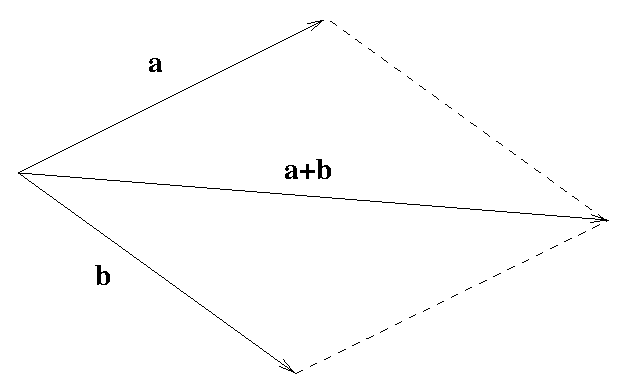
\includegraphics[scale=0.5]{immagini/fisica1/somma_vettori}
\caption{Regola del parallelogramma}
\end{figure}



\subsubsection{Differenza} La differenza di due
vettori è la somma del primo con l'inverso del secondo. Graficamente $\ve a-\ve b$ è il vettore che congiunge $\ve b$ ad $\ve a$.
\subsubsection{Prodotto per uno scalare}
Per via geometrica il prodotto scalare di un vettore per uno scalare corrisponde al vettore con stessa direzione, con modulo moltiplicato per il valore assoluto dello scalare e verso invertito se lo scalare è negativo.
\begin{equation*}\forall h \in \field{R}\qquad h\ve a=h(a_x\ve i+a_y\ve j+a_z\ve k)=ha_x\ve i+ha_y\ve j+ha_z\ve k\end{equation*}
\subsubsection{\index{prodotto!scalare}Prodotto scalare}
Il prodotto scalare usato in fisica è il prodotto scalare canonico della geometria in $\field{R}^3$ rispetto alla base canonica $\{\ve i,\ve j,\ve k\}$:
\begin{equation*}\left(\ve{x},\ve{y}\right)=\ve{x}^T\cdot\ve{y}=(x_1y_1+x_2y_2+x_3y_3)\end{equation*}
\begin{equation*}p_s=|\ve a||\ve b| \cos \alpha\end{equation*}
 con $\alpha$ l'angolo compreso tra i due vettori. Da qui si deduce che $\ve i \cdot \ve i=1$, $\ve i
\cdot \ve j=0$, ecc., che due vettori ortogonali hanno prodotto scalare nullo e che due vettori hanno prodotto scalare massimo quando sono paralleli.
$$p_s=\ve a \cdot \ve b=(a_x\ve i+a_y\ve j+a_z\ve k)\cdot(b_x\ve
i+b_y\ve j+b_z\ve k)=a_xb_x+a_yb_y+a_zb_z$$
\subsubsection{\index{prodotto!vettoriale}Prodotto Vettoriale}
Matematicamente il prodotto vettoriale non è facile da definire. Esso restituisce un vettore che ha direzione ortogonale al piano individuato dai due vettori, verso ricavabile dalla regola della mano destra, e modulo:
\begin{equation*}|\ve p_v|=ab\sin \alpha\end{equation*} con $\alpha$ angolo tra i due vettori\footnote{è molto semplice ricordarsi la formula del prodotto vettoriale, basta ciclare sulle variabili. Per esempio la componente $x$ del prodotto vettoriale è $a_yb_z-a_zb_y$ in cui l'ordine è $x$ (la componente) e poi $y$, $z$, seguito dalla sottrazione al contrario (è antisimmetrico)}.


\begin{align*}
\ve p_v&=\ve a \wedge \ve b=\ve a \times \ve b=(a_x\ve i+a_y\ve j+a_z\ve k)\wedge(b_x\ve
i+b_y\ve j+b_z\ve k)\\
&=(a_yb_z-a_zb_y)\ve i+(a_zb_x-a_xb_z)\ve j+(a_xb_y-a_yb_x)\ve k
\end{align*}

Il prodotto scalare può essere calcolato come determinante di una matrice $3\times 3$:
$$\ve p_v=
\left| \begin{array}{ccc} \ve i & \ve j & \ve k\\
a_x & a_y & a_z\\
b_x & b_y& b_z
 \end{array} \right|$$

Il prodotto vettoriale è antisimmetrico cioè $\ve a \wedge \ve
b=-\left(\ve b \wedge \ve a\right)$. Il modulo del prodotto
vettoriale è l'area del parallelogramma avente come lati i due
vettori.

Il prodotto vettoriale è dipendente dalla scelta del sistema di riferimento. In particolare il verso del prodotto vettoriale segue la regola della mano destra se il sistema di riferimento è destrogiro, altrimenti il verso risulta opposto. Per questo il prodotto vettoriale è chiamato pseudovettore. In natura le grandezze osservabili non devono dipendere dalla scelta dell'orientazione (chiralità) degli assi cartesiani. Per convenzione si sceglie un sistema di riferimento destrogiro.
\begin{figure}[htbp]
\centering
\subfigure[destrogiro]{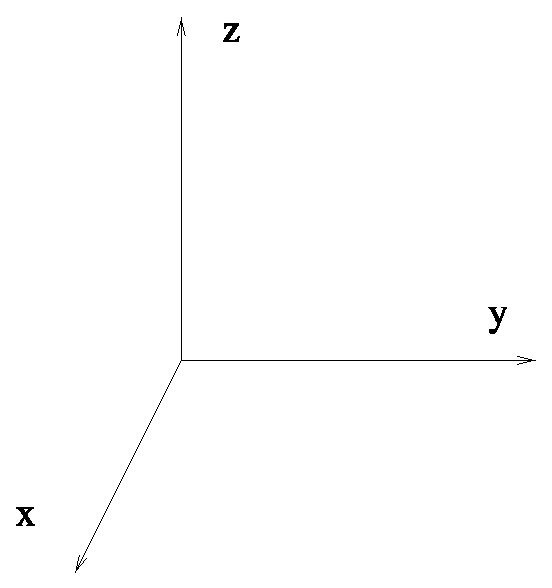
\includegraphics[scale=0.5]{immagini/fisica1/sistema_destrogiro}}
\subfigure[sinistrogiro]{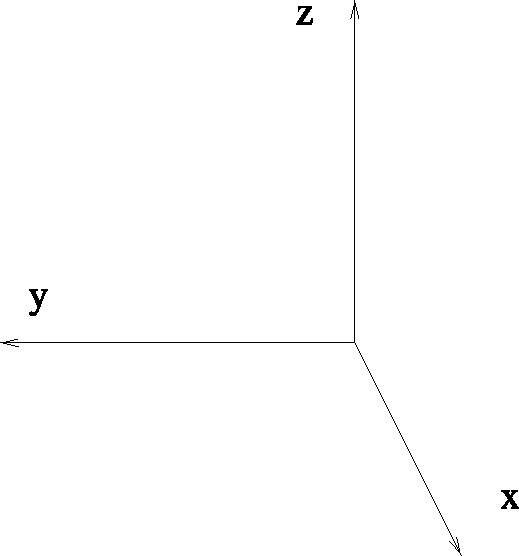
\includegraphics[scale=0.5]{immagini/fisica1/sistema_sinistrogiro}}
\end{figure}

\subsubsection{\index{prodotto!misto}Prodotto Misto}
Il prodotto misto è definito come:
\begin{equation*}p_m=\ve c\cdot\left(\ve a \wedge \ve b\right)\end{equation*}
Esso è uguale all'area del parallelepipedo avente come spigoli i
vettori \mbox{$\ve a$, $\ve b$, $\ve c$.}

\subsubsection{\index{derivata!di un vettore}Derivata di un vettore}
La derivata di un vettore è la derivata delle coordinate per i rispettivi versori, (i versori sono costanti). Per esempio la derivata della velocità rispetto al tempo è:
\begin{equation*}\frac{\ud\ve v}{\ud t}=\frac{\ud v_x}{\ud t}\ve i+\frac{\ud v_y}{\ud t}\ve j+\frac{\ud v_z}{\ud t}\ve k\end{equation*}

\subsubsection{\index{gradiente}Gradiente}
\label{gradiente}
Il gradiente di uno scalare è definito come:
\begin{equation*}
\grad V(x,y,z)=\ve\nabla V(x,y,z)=\frac{\partial V}{\partial x}\ver i + \frac{\partial V}{\partial y}\ver j +\frac{\partial V}{\partial z}\ver k +
\end{equation*}
dove $\ve\nabla$ è un operatore definito come:
\begin{equation*}
\ve\nabla=\left(\frac{\partial}{\partial x},\frac{\partial}{\partial y},\frac{\partial }{\partial z}\right)
\end{equation*}
con questo operatore abbiamo il divertimento di scrivere le nostre formule per esempio in questo modo:

\begin{equation*}
\ve F=-\ve\nabla U
\end{equation*}
invece di:
\begin{equation*}
\ve F=-\left(\frac{\partial U}{\partial
x}\ve i+\frac{\partial U}{\partial y}\ve j+\frac{\partial
U}{\partial z}\ve k\right)
\end{equation*}

\chapter{Cinematica}
\section{\index{posizione}Vettore posizione}
Fissato un sistema di riferimento cartesiano\footnote{per semplicità quasi sempre si parlerà del piano piuttosto che dello spazio, ma i risultati sono del tutto analoghi} $Oxy$ il vettore che congiunge l'origine con un punto $P$ è il vettore posizione $\ve r$ che individua $P$ in quel sistema di riferimento. Poiché il punto può spostarsi nel tempo $\ve r$ sarà funzione del tempo $\ve r=\ve r(t)$ e descriverà al variare del tempo tutte le posizioni occupate da $P$ cioè la sua traiettoria.

\begin{figure}[htbp]
\centering
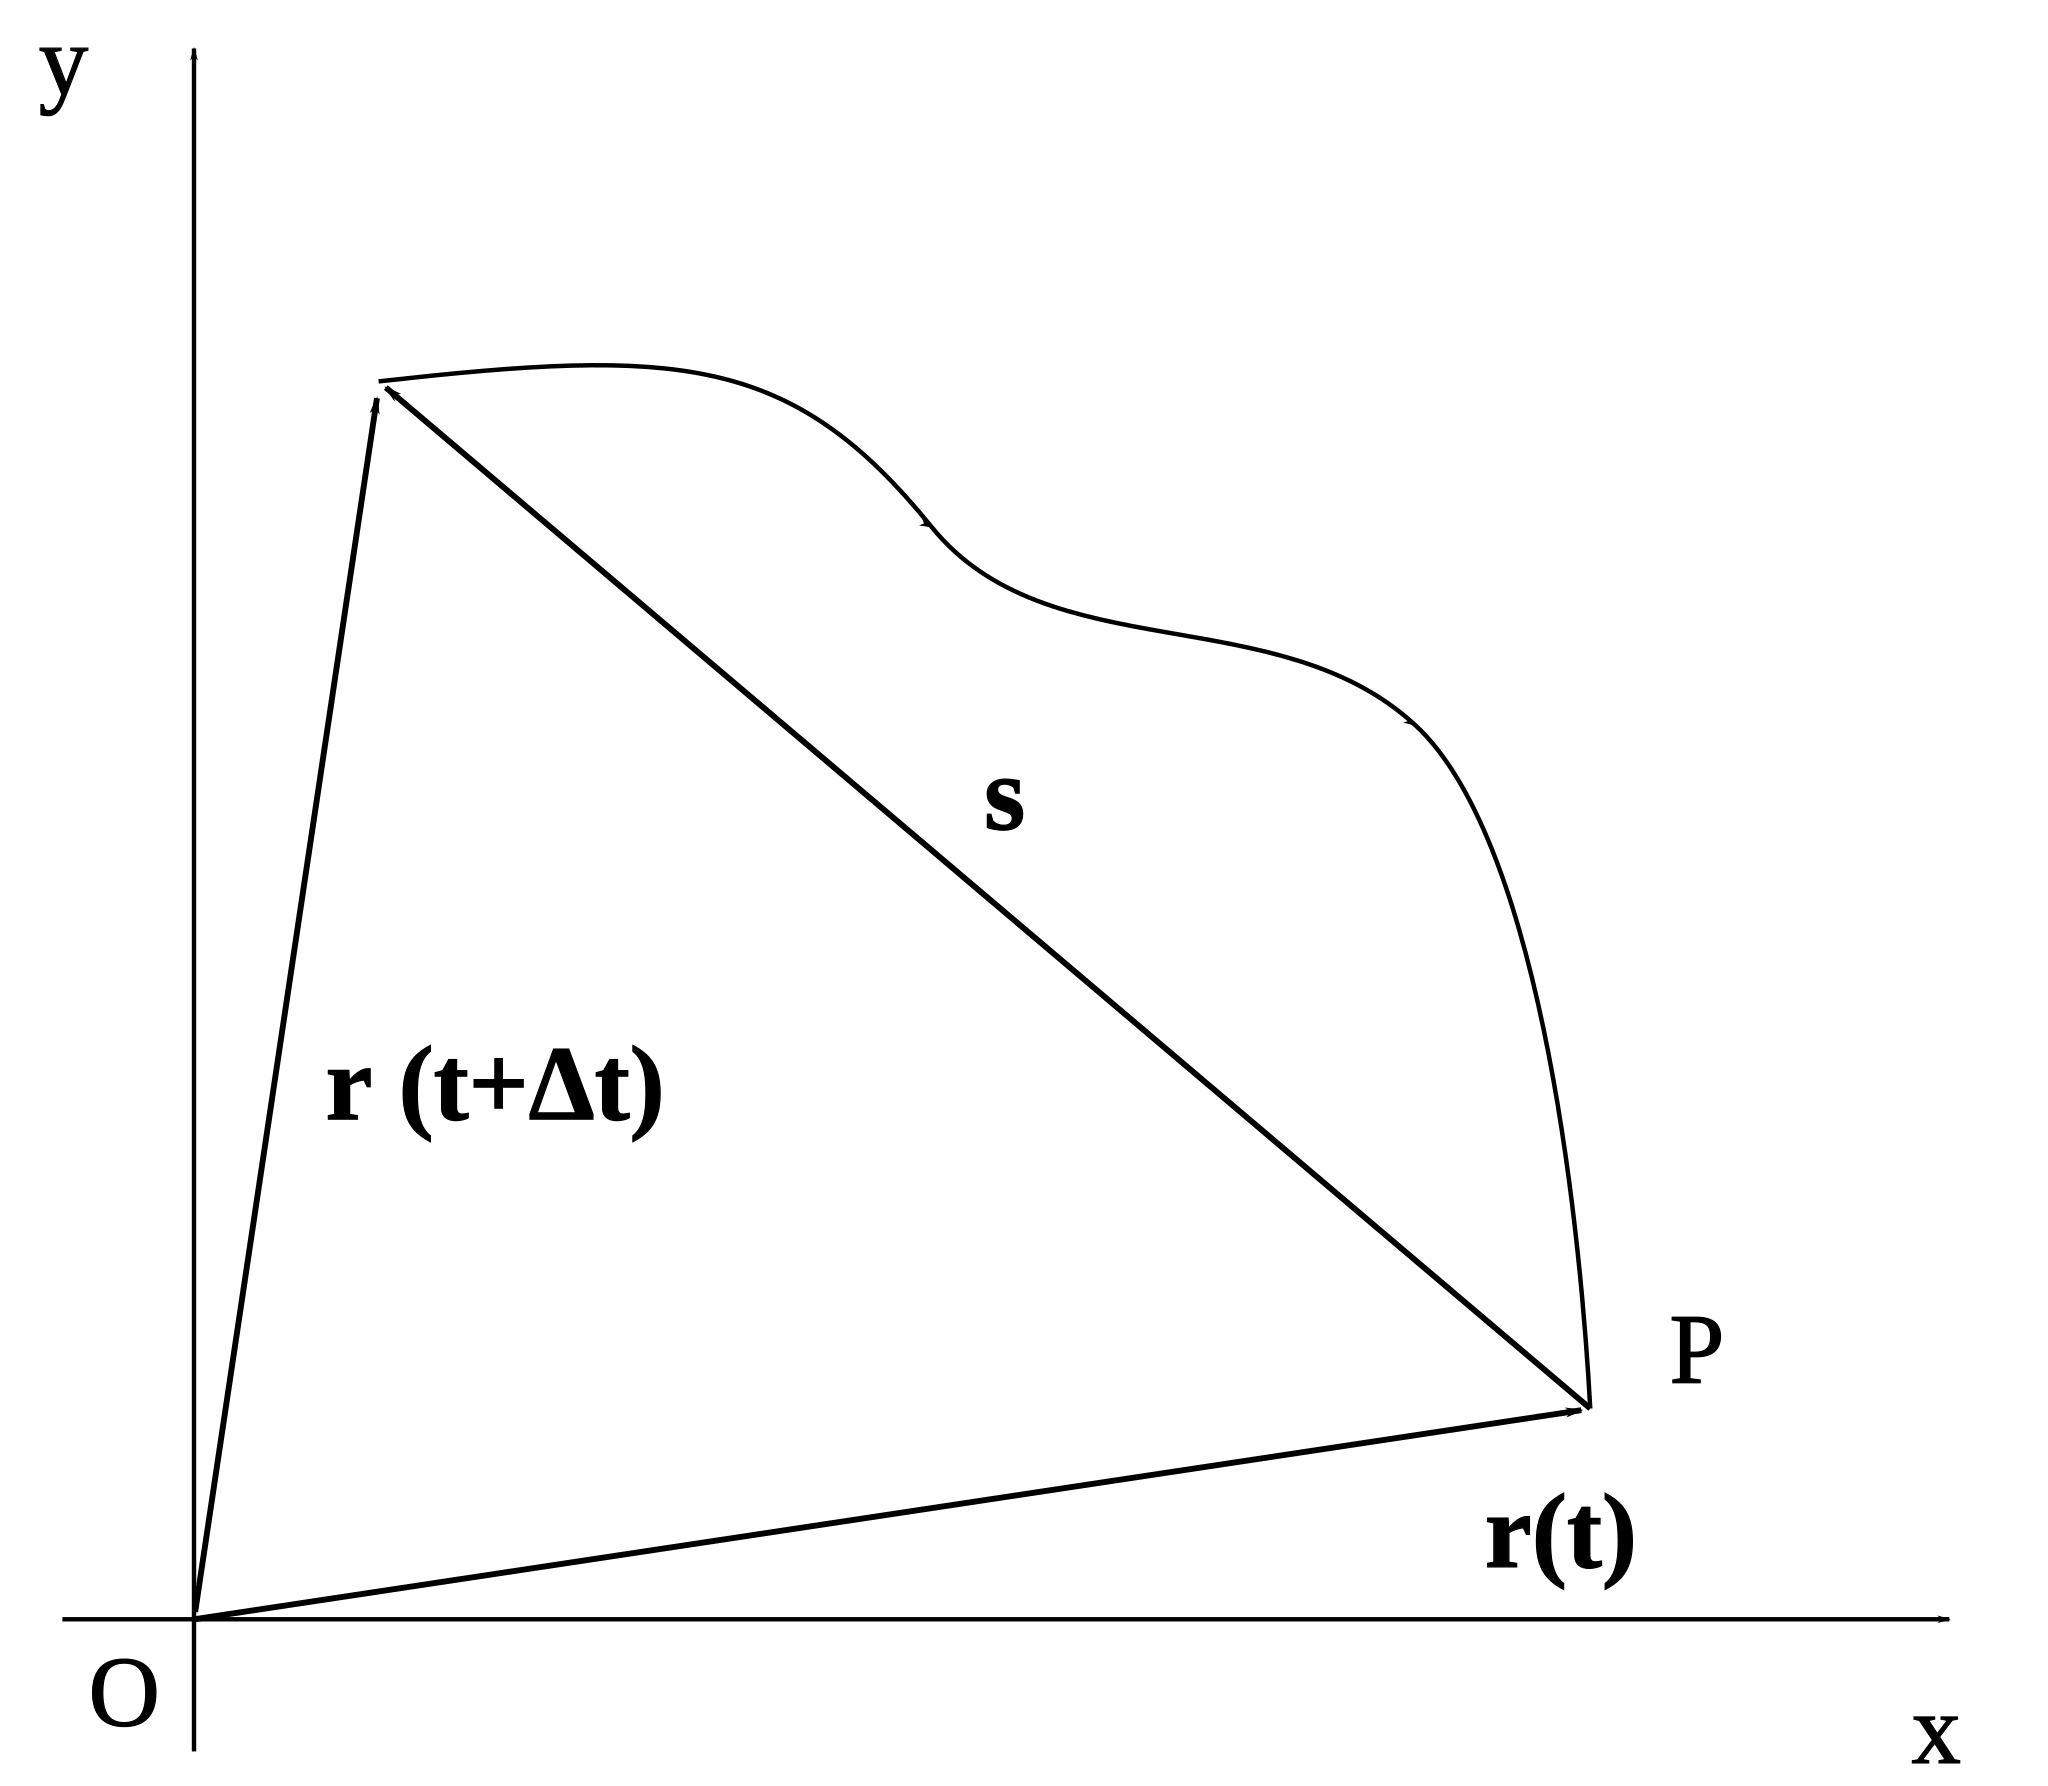
\includegraphics[scale=0.7]{immagini/fisica1/vettore_posizione}
\caption{vettore posizione e spostamento}
\end{figure}
\subsection{Vettore spostamento}
\parbox[c]{\textwidth}{
\begin{align*}
\ve s\left(t,\Delta t\right)&=\Delta \ve r(t,\Delta t)\\
&=\ve r\left(t+\Delta t\right)-\ve r\left(t\right)=x\left(t+\Delta t\right)\ve i+y\left(t+\Delta t\right)\ve j-x\left(t\right)\ve i-y\left(t\right)\ve j\\
&=\left[x(t+\Delta t)-x(\Delta t)\right]\ve i+[y(t+\Delta t)-y(t)]\ve j=\Delta x\ve i+\Delta y \ve j
\end{align*}
}
\section{\index{velocità}Vettore velocità}
\begin{Def}[\index{velocità!media}Velocità Media]
$$\ve v_m(t,t+\Delta t)=\frac{\Delta\ve r(t+\Delta t)}{\Delta
t}=\frac{1}{\Delta t}\{\Delta x\ve i+\Delta y\ve
j\}=\frac{\Delta x}{\Delta t}\ve i+\frac{\Delta y}{\Delta t}\ve
j$$
\end{Def}
\begin{Def}[\index{velocità!istantanea}Velocità Istantanea]
\begin{equation*}\ve v(t)=\lim_{\Delta t\rightarrow 0}\ve v_m(t,t+\Delta t)=\lim_{\Delta t\rightarrow 0} \frac{\Delta\ve r}{\Delta t}(t)={\left.\frac{\ud \ve r}{\ud t}\right|_t}=\left.\frac{\ud x}{\ud t}\right|_t\ve i+\left.\frac{\ud y}{\ud t}\right|_t\ve j\end{equation*}
\end{Def}
\begin{equation*}\norm{\ve v}=\norm{\frac{\ud\ve r}{\ud t}}\neq\frac{\ud}{\ud t}\norm{\ve r}\end{equation*}
\begin{Def}[\index{velocità!scalare}Velocità Scalare]
\begin{equation*}v_s=\frac{\text{spazio totale percorso}}{\Delta t}\end{equation*}
\end{Def}
\section{\index{accelerazione}Vettore accelerazione}
\begin{Def}[accelerazione istantanea]
\begin{equation*}\ve a(t)=\frac{\ud \ve v}{\ud t}(t)={\frac{\ud^2 \ve r}{\ud t^2}}(t)\end{equation*}
\end{Def}
\section[Moto rettilineo uniforme]{\index{moto!rettilineo uniforme}Moto rettilineo uniforme\protect\footnote{usiamo sempre condizioni iniziali implicite, del tipo $t_0=0$, $\ve r(0)=\ve r_0$, $\ve v(0)=\ve v_0$}}
\begin{equation*}\frac{\ud\ve r}{\ud t}=\ve v=\overrightarrow\const\end{equation*}
\begin{equation*}\ud\ve r=\ve v\,\ud t\qquad\int_{\ve r_0}^{\ve r}\ud\ve r=\int_0^t\ve v\,\ud t\end{equation*}
\begin{equation*}\ve r-\ve r_0=\ve v t\qquad\ve r=\ve v t+\ve r_0\end{equation*}
\section{\index{moto!uniformemente accelerato}Moto uniformemente accelerato}
\begin{equation*}\frac{\ud \ve v}{\ud t}=\ve a=\overrightarrow{\const}\end{equation*}
\begin{equation*}\ve a\,\ud t=\ud \ve v\qquad\int_0^t\ve a\,\ud t=\int_{\ve v_0}^{\ve v}\ud \ve v\qquad\ve a t=\ve v-\ve v_0\end{equation*}
\begin{equation}
\ve v=\ve a t+\ve v_0
\label{vt_01}
\end{equation}
\begin{equation*}\ve v=\ve a t+\ve v_0=\frac{\ud \ve r}{\ud t}\end{equation*}
\begin{equation*}\ud \ve r=\left(\ve a t+\ve v_0\right)\ud t\qquad\int_{\ve r_0}^{\ve r}\ud \ve r=\int_0^t\left(\ve a t+\ve v_0\right)\ud t\qquad\ve r-\ve r_0=\frac{1}{2}\ve a t^2+\ve v_0 t\end{equation*}
\begin{equation}
\ve r=\frac{1}{2}\ve a t^2+\ve v_0 t+\ve r_0
\label{vt_02}
\end{equation}
\subsection{Velocità in funzione dello spazio}
In certi casi può risultare molto comoda la formula relativa al
moto uniformemente accelerato scritta in questo modo:
\begin{equation}
v^2-v_0^2=2a(r-r_0)
\label{vt_03}
\end{equation}
che vale solo nel caso unidimensionale\footnote{nel caso unidimensionale le \eqref{vt_01} e la \eqref{vt_02} si scrivono come:
\begin{equation}
v(t)=at+v_0\qquad r(t)=\frac{1}{2}at^2+v_0t+r_0
\end{equation}
eliminiamo il tempo per trovare $v(r)$: ricaviamo $t$ dalla prima e sostituiamolo nella seconda, semplifichiamo e otteniamo la \eqref{vt_03}}.
\section{\index{moto!circolare!uniforme}Moto circolare uniforme}
Per moto circolare uniforme si intende quel moto su traiettoria
circolare in cui il modulo del vettore velocità rimane costante
nel tempo (mentre la sua direzione varia ed è sempre tangente
alla circonferenza). Definiamo la velocità angolare\index{velocità!angolare}\index{omega@$\omega$|see{velocità angolare}}: $\omega=\frac{\ud\theta}{\ud t}$ e l'accelerazione angolare\index{accelerazione!angolare}\index{alpha@$\alpha$|see{accelerazione angolare}} $\alpha=\frac{\ud \omega}{\ud t}$; in realtà sono dei vettori.
\begin{equation*}\left|\ve v\right|=\const\end{equation*}
\begin{equation*}\text{scegliamo $\ve r_0$}:\left\{
\begin{array}{l}
x=R\\
y=0\\
\end{array}\right.\end{equation*}
\begin{equation*}\ve r=R\cos\theta\ve i+R\sin\theta\ve j\end{equation*}
\begin{equation*}\theta=\frac{\text{arco}}{\text{raggio}}=\frac{vt}{R}=\omega t\qquad\omega=\dot\theta=\frac{v}{R}=\const\end{equation*}
\begin{equation*}\ve r=R\cos(\omega t)\ve i+R\sin(\omega t)\ve j\end{equation*}
\begin{equation*}\ve v=\frac{\ud \ve r}{\ud t}=-R\omega\sin(\omega t)\ve
i+R\omega\cos(\omega t)\ve j\end{equation*}
\begin{align*}|\ve v|^2&=v_x^2+v_y^2=R^2\omega^2\sin^2(\omega
t)+R^2\omega^2\cos^2(\omega t)\\
&=R^2\omega^2\left(\sin^2\left(\omega t\right)+\cos^2\left(\omega
t\right)\right)=R^2\omega^2
\end{align*}
\begin{equation*}v=\omega R\end{equation*}
\begin{equation*}\ve v\cdot\ve r=0\Rightarrow\ve v\bot\ve r\end{equation*}
\begin{equation*}\ve v\cdot\ve r=v_xx+v_yy=-R\omega\sin(\omega t)R\cos(\omega t)+R\omega\cos(\omega t)R\sin(\omega t)=0\end{equation*}
\begin{align*}
\ve a&=\frac{\ud\ve v}{\ud t}=-R\omega^2\cos(\omega t)\ve
i-R\omega^2\sin(\omega t)\ve j\\
&=-R\omega^2\left(\cos\left(\omega t\right)\ve i+
\sin\left(\omega t\right)\ve j\right)=-\omega^2\ve r
\end{align*}
\begin{equation*}|\ve a|^2=R^2\omega^4\cos^2(\omega t)+R^2\omega^4\sin^2(\omega
t)=R^2\omega^4\end{equation*}
\begin{equation*}a=\omega^2R=\omega v=\frac{v^2}{R}\end{equation*}
\section{\index{moto!circolare}Moto circolare}
\begin{figure}[htbp]
\centering
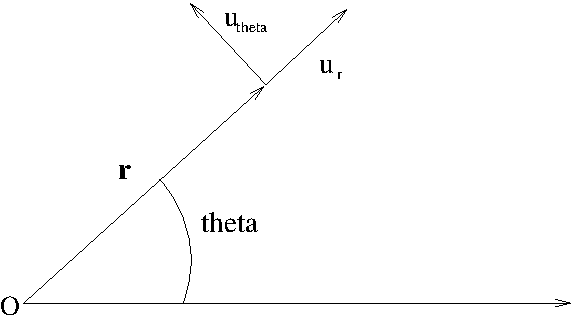
\includegraphics[scale=1]{immagini/fisica1/CorPol}
\caption{\index{coordinate!polari}Coordinate polari}
\end{figure}
\begin{equation*}\ve r=R\ve u_r\end{equation*}
\begin{equation*}
\left\{\begin{array}{ll}
\ve u_r=\cos\theta(t)\ve i+\sin\theta(t)\ve j\\
\ve u_\theta=-\sin\theta(t)\ve i+\cos\theta(t)\ve j
\end{array}\right.
\end{equation*}
\begin{equation*}\frac{\ud\ve u_\theta}{\ud t}=-\dot{\theta}\cos\theta\ve i-\dot{\theta}\sin\theta\ve j=-\dot{\theta}\ve u_r\end{equation*}
\begin{align*}
\ve v&=\frac{\ud \ve r}{\ud t}=\frac{\ud\left(R\ve
u_r\right)}{\ud t}=R\frac{\ud \ve u_r}{\ud
t}\\
&=R\left(-\dot\theta\sin\theta\ve i+\dot\theta\cos\theta\ve
j\right)=R\dot\theta\ve u_\theta
\end{align*}
$$\ve a=\frac{\ud\ve v}{\ud t}=\frac{\ud\left(R\dot\theta\ve
u_\theta\right)}{\ud t}=R\ddot\theta\ve
u_\theta+R\dot\theta\frac{\ud\ve u_\theta}{\ud
t}=R\ddot\theta\ve u_\theta-R\dot\theta^2\ve u_r$$


\section{\index{moto!in coordinate polari}Moto qualsiasi in coordinate polari}
\begin{equation*}\ve r(t)=r\ve u_r\end{equation*}
\begin{equation*}\ve u_r=\cos\theta\ve i+\sin\theta\ve j\qquad \ve u_\theta=-\sin\theta\ve i+\cos\theta\ve j\end{equation*}
$$\frac{\ud\ve u_r}{\ud t}=-\dot\theta\sin\theta\ve
i+\dot\theta\cos\theta\ve j=\dot\theta\left(-\sin\theta\ve
i+\cos\theta\ve j\right)=\dot\theta\ve u_\theta$$
$$\frac{\ud\ve u_\theta}{\ud t}=-\dot\theta\cos\theta\ve
i-\dot\theta\cos\theta\ve j=-\dot\theta\left(\cos\theta\ve
i+\sin\theta\ve j\right)=-\dot\theta\ve u_r$$
$$\ve v=\frac{\ud\ve r}{\ud t}=\dot r\ve u_r+r\frac{\ud\ve
u_r}{\ud t}=\dot r\ve u_r+r\dot\theta\ve u_\theta$$
$$\ve a=\frac{\ud\ve v}{\ud t}=\ddot r\ve u_r+\dot
r\dot\theta\ve u_\theta+\dot r\dot\theta\ve
u_\theta+r\ddot\theta\ve u_\theta-r\dot\theta^2\ve u_r=\ve
u_r\left(\ddot r-r\dot\theta^2\right)+\ve u_\theta\left(2\dot
r\dot\theta+r\ddot\theta\right)$$

 I vettori velocità e accelerazione vengono scomposti in due
componenti:
\begin{enumerate}
\item[--] \index{velocità!radiale}Velocità radiale: $v_r=\dot r$
\item[--] \index{velocità!perpendicolare}Velocità perpendicolare: $v_\theta=r\dot\theta$
\item[--] \index{accelerazione!radiale}Accelerazione radiale: $a_r=\ddot r-r\dot\theta^2$
\item[--] \index{accelerazione!perpendicolare}Accelerazione perpendicolare: $a_\theta=2\dot r\dot\theta+r\ddot
\theta$
\end{enumerate}
\section{\index{moto!armonico}Moto armonico}
Il moto armonico è un moto con equazione differenziale:
\begin{equation*}\ddot x=-k x\end{equation*}
cioè:
\begin{equation*}x=A\sin(\omega t+\varphi)\end{equation*}
\begin{equation*}v=\frac{\ud x}{\ud t}=A\omega\cos(\omega t+\varphi)\end{equation*}
\begin{equation*}a=\frac{\ud v}{\ud t}=-A\omega^2\sin(\omega t+\varphi)=-\omega^2 x=\ddot x\end{equation*}
\begin{equation*}k=\frac{1}{\omega^2}\qquad x=-\frac{1}{\omega^2}\ddot x\end{equation*}
 Per esempi (pendoli, molle) vedi sezione \ref{armonico} a
pagina \pageref{armonico}
\subsection{Moto armonico smorzato\index{moto!armonico!smorzato}}
Introduciamo nel moto armonico una forza smorzatrice, per esempio una forza d'attrito che varia con la velocità:
\begin{equation*}F=-\gamma \frac{\ud x}{\ud t}\end{equation*}
\begin{equation*}m\ddot x=-kx-\gamma\dot x\qquad m\ddot x+\gamma\dot x+kx=0\end{equation*}
$\tau=\frac{m}{\gamma}$ è un tempo, la frequenza del moto armonico non smorzato è $\frac{k}{m}=\omega_0^2$
\begin{equation*}\ddot x+\frac{\gamma}{m}\dot x+\frac{k}{m}x=0\qquad \ddot x+\frac{1}{\tau}\dot x+\omega_0^2x=0\end{equation*}
se $\tau=\infty$ allora il moto non è più smorzato.

Una soluzione è:
\begin{equation*}x(t)=e^{st}\end{equation*}
\begin{equation*}\dot x(t)=sx(t)\qquad \ddot x(t)=s^2x(t)\end{equation*}
\begin{equation*}s^2x(t)+\frac{1}{\tau}sx(t)+\omega_0^2x(t)=0\end{equation*}
\begin{equation*}s_{1/2}=\dfrac{-\dfrac{1}{\tau}\pm\sqrt{\dfrac{1}{\tau^2}-4\omega_0^2}}{2}=-\frac{1}{2\tau}\pm\sqrt{\frac{1}{4\tau^2}-\omega_0^2}\end{equation*}
quindi la soluzione generale è una combinazione lineare delle soluzioni:
\begin{equation*}
 x(t)=A_1e^{s_1t}+A_2e^{s_2t}
\end{equation*}
a seconda che le radici del polinomio siano reali o complesse si possono distinguere due casi:
\begin{description}
\item[attrito forte]
\begin{equation*}\beta=\frac{1}{4\tau^2}-\omega_0^2>0\qquad\tau<\frac{1}{2\omega_0}\qquad\gamma>2\sqrt{km}\end{equation*}
\begin{equation*}s_{1/2}=-\frac{1}{2\tau}\pm\beta\qquad\text{radici reali e}<0\end{equation*}
\begin{equation*}x(t)=A_1e^{s_1t}+A_2e^{s_2t}\end{equation*}
\item[attrito debole]
\begin{equation*}\frac{1}{4\tau^2}-\omega_0^2<0\qquad \tau>\frac{1}{2\omega_0}\qquad\gamma<2\sqrt{km}\end{equation*}
\begin{equation*}s_{1/2}=\dfrac{-\dfrac{1}{\tau}\pm\sqrt{\dfrac{1}{\tau^2}-4\omega_0^2}}{2}=-\frac{1}{2\tau}\pm i\omega\end{equation*}
\begin{align*}x(t)&=A_1e^{s_1it}+A_2e^{s_2it}=A_1e^{-\frac{t}{2\tau}-i\omega t}+A_2e^{-\frac{t}{2\tau}+i\omega t}=\\
&=e^{-\frac{t}{2\tau}}\left(A_1e^{-i\omega t}+A_2e^{i\omega t}\right)=A e^{-\frac{t}{2\tau}}\sin(\omega t +\varphi)\end{align*}
quindi è un moto armonico con frequenza $\omega=\sqrt{\omega_0-\frac{1}{4\tau^2}}$ la cui ampiezza diminuisce con un fattore frenante $e^{-\frac{t}{2\tau}}$.\footnote{Il caso in cui ci siano due radici coincidenti è tralasciato poiché puntiforme}
\end{description}

\section{\index{trasformazioni!di Galileo}Trasformazioni di Galileo}
Le trasformazioni di Galileo sono equazioni valide nella meccanica classica che consentono di descrivere le coordinate di un sistema rispetto alle di coordinate di un altro sistema che si muove di moto rettilineo uniforme rispetto al primo. Un sistema è detto inerziale se vale la prima legge di Newton. Se in un sistema è inerziale allora un altro sistema è inerziale se e solo se si muove di motto rettilineo uniforme rispetto al primo.
\newline

Primo osservatore ``fermo'':$\qquad O\quad\ve r\quad\;\ve
v\quad\;\ve a$

Secondo osservatore in moto:$\:\quad O'\quad\!\ve r\,'\quad\!\ve
v\,'\quad\!\ve a\,'$

In meccanica classica si assume:$\quad t=t'$

$\ve u$ velocità di trascinamento: \index{velocità!relativa}velocità di $O'$ rispetto ad $O$.
\begin{legge}
$\ve r(t)=\overrightarrow{\left(O'-O\right)}+\ve r\,'=\ve u
t+\ve r\,'$
\end{legge}
\begin{legge}[composizione delle velocità]
\index{composizione delle velocità}
$$\ve v=\frac{\ud\ve r}{\ud t}=\frac{\ud}{\ud t}\left(\ve u
t+\ve r\,'\right)=\frac{d}{\ud t}\left(\ve u
t\right)+\frac{\ud\ve r\,'}{\ud t}=\ve u+\frac{\ud\ve r\,'}{\ud
t'}=\ve u+\ve v\,'$$
velocità assoluta = velocità relativa + \index{velocità!di trascinamento}velocità di trascinamento
\end{legge}
\begin{legge}[invarianza dell'accelerazione]
$$\ve a=\frac{\ud \ve v}{\ud t}=\frac{\ud}{\ud t}(\ve u+\ve
v\,')=0+\frac{\ud \ve v\,'}{\ud t}=\frac{\ud \ve v\,'}{\ud
t'}=\ve a'$$
L'accelerazione quindi è invariante
\end{legge}
$$\left\{\begin{array}{ll}
\ve r=\ve r\,'+\ve u t&\text{trasformate di Galileo}\\
\ve v=\ve u+\ve v\,'&\text{somma delle velocità}\\
\ve a=\ve a\,'&\text{invarianza dell'accelerazione}\\
t=t'&\text{ipotesi del tempo assoluto}\\
\end{array}\right.$$
Esse valgono nell'ipotesi che se $t=0=t'$ allora $\ve r\,'=\ve r$.
Non esiste un sistema di riferimento assoluto.
\subsection{Invarianza e covarianza\index{invarianza}\index{covarianza}}
Una grandezza si dice invariante se è numericamente uguale alla sua trasformata, cioè $x=T(x)=x'$. Nelle trasformazioni di Galileo l'accelerazione è invariante rispetto alla trasformazione che trasforma le coordinate di $O$ in quelle di $O'$. Nella relatività galileiana la lunghezza è invariante, nella relatività ristretta no.

Una legge si dice covariante se la sua espressione è uguale alla sua trasformata, cioè $f(x)=T(f(x))$.




\chapter{Dinamica}

\section{\index{forza!fondamentale}Forze fondamentali}
\begin{enumerate}
\item forza gravitazionale
\item forza elettromagnetica
\item forza nucleare debole
\item forza nucleare forte
\end{enumerate}
Tutte le altre forze non sono altro che combinazioni di queste.
\section{Altre forze}
Molte forze sono descritte con leggi che approssimano il loro comportamento, consentendo un'analisi dinamica del sistema, senza dover considerare direttamente le forze fondamentali.

\subsection{\index{forza!elastica}Forza elastica}
\begin{legge}[Hook]
\begin{equation*}
\ve F=-k\Delta\ve x
\end{equation*}
 con $\Delta\ve x$ l'allungamento. Questa legge è valida per i corpi elastici e per allungamenti limitati, dopo di che il corpo non si comporta più in modo elastico e rimane deformato.
\end{legge}

\subsection{\index{resistenza!del mezzo}Resistenza del mezzo}
La resistenza del mezzo è quella forza che il fluido in cui è
immerso un corpo in movimento esercita sul corpo. La forza è
proporzionale alla velocità, ma può essere anche proporzionale al
quadrato della velocità.
\begin{equation*}
\ve F=-k\mu \ve v
\end{equation*}
oppure:
\begin{equation*}
\ve F=-k\mu v\ve v
\end{equation*}
dove $\mu$ dipende dalla geometria del corpo,
$k$ dalla natura del mezzo.
\subsection{\index{attrito!statico}Attrito statico}
Le leggi sull'attrito vengono chiamate leggi di Leonardo\index{leggi!di Leonardo}\index{Leonardo}.
\begin{legge}[Prima legge di Leonardo]
$f_s\leq\mu_s N$ con $\mu_s$coefficiente di attrito statico
\end{legge}
\begin{legge}[Seconda legge di Leonardo]
La forza di attrito è indipendente dalla superficie d'appoggio
\end{legge}
\subsection{\index{attrito!dinamico}Attrito dinamico}
\begin{equation*}
F_c=\mu_cN
\end{equation*}
$\mu_c=$ coefficiente di attrito dinamico. $\mu_c<\mu_s$

\section{\index{principi della dinamica}Leggi di Newton}
Le leggi di Newton sono i principi della dinamica, legano due mondi distinti, quello del mondo esterno e quello della cinematica attraverso le forze. In quanto principi non hanno nessuna giustificazione, se non la verifica sperimentale.
\begin{Pri}[Primo principio della dinamica]
Quando un corpo è sottoposto ad una forza risultante nulla è
possibile individuare una classe di riferimenti rispetto ai quali
la sua accelerazione è zero (e si chiama classe dei sistemi inerziali).
\end{Pri}
\begin{Pri}[Secondo principio della dinamica]
\begin{equation}
\sum\ve F=m\ve a
\label{sec_din}
\end{equation}
\end{Pri}
In realtà Newton formulò questa espressione come $\sum \ve
F=\frac{\ud \ve p}{\ud t}$
\begin{Pri}[Terzo principio della dinamica]
Se un corpo esercita una forza su un altro corpo, il secondo corpo
esercita una forza sul primo. Queste due forze sono uguali in
modulo, hanno la stessa direzione e versi opposti.
\end{Pri}


\section{\index{forza!variabile}Forze variabili}
In generale la forza è una funzione del tipo:
\begin{equation}
\ve F=\ve F(\ve r,\ve v,t)
\label{f_din}
\end{equation}
La risoluzione dell'equazione differenziale \eqref{sec_din} con la forza data dalla \eqref{f_din} è compito della meccanica. Il caso più semplice è quello in cui $\ve F$ è una costante, vediamo degli esempi in cui non lo è.
\subsection{\index{forza!variabile!nel tempo}Forze variabili nel tempo}
\begin{Es}
Una macchina viaggia alla velocità di \unita{100}\kilo\meter\per\hour, la forza dei freni
varia nel tempo e quindi l'accelerazione impressa dai freni segue
la legge $a=ct$ con $c=\unita{-3}\meter\per\cubic\second$. Quanto ci mette la
macchina a fermarsi?
\newline
\newline $v_0=\unita{100}\kilo\metre\per\hour\simeq \unita{27.7}\metrepersecond$
\newline $c=\unita{-3}\meter\per\cubic\second$
\newline $a=ct$
\newline $F=ma=mct$

Il risultato si trova integrando le definizioni di accelerazione, velocità e spazio.
$$a=\frac{\ud v}{\ud t}=ct \quad \Rightarrow \quad\ud v=ct\,\ud
t\quad\Rightarrow\quad\int_{v_0}^v\ud v=\int_0^t ct\,\ud t$$
\begin{equation*}v-v_0=\frac{ct^2}{2}\qquad v=\frac{ct^2}{2}+v_0\end{equation*}
$$v=\frac{\ud x}{\ud t}\qquad\int_0^t v\,\ud t=\int_0^x\ud
x\qquad\int_0^t\frac{ct^2}{2}+v_0\,\ud t=\int_0^x\ud x$$
\begin{equation*}\frac{ct^3}{6}+v_0t=x\qquad x=v_0t+\frac{ct^3}{6}\end{equation*}
$$v_f=0\qquad v_f=0=\frac{ct^2}{2}+v_0\qquad
t=\sqrt{\frac{-2v_0}{c}}\simeq \unita{4.30}\second$$
\end{Es}

\subsection{\index{forza!variabile!nello spazio}Forze variabili nello spazio}
\subsubsection{Moto armonico delle molle}
\label{armonico}

\begin{equation}F=-kx=ma\end{equation}
\begin{equation*}a=\frac{\ud v}{\ud t}=\frac{\ud^2 x}{\ud t^2}\end{equation*}
$$-kx=m\frac{\ud^2 x}{\ud t^2}\qquad m\frac{\ud^2 x}{\ud
t}+kx=0\qquad x=-\frac{m\ddot x}{k}$$
la soluzione generale è del tipo:
\begin{equation}x(t)=A\sin(\omega t+\varphi)\end{equation}
con $\omega=\sqrt{\frac{k}{m}}$, da cui si può ricavare anche:
\begin{equation*}\dot x(t)=A\omega\cos(\omega t+\varphi)\end{equation*}
\begin{equation*}\ddot x(t)=-A\omega^2\sin(\omega t+\varphi)=\omega^2x\end{equation*}
\begin{equation*}x=-\frac{1}{\omega^2}\ddot x\end{equation*}
confrontando questa funzione con quella trovata prima si ha che:
$$\frac{1}{\omega^2}=\frac{m}{k}\qquad \omega^2=\frac{k}{m}\qquad
\omega=\sqrt{\frac{k}{m}}$$
come già accennato. L'equazione del moto è quindi:
\begin{equation}
x=A\sin\left(\sqrt{\frac{k}{m}}\,t+\varphi\right)
\end{equation}
le costanti $A$ e $\varphi$ sono da trovarsi con le condizioni iniziali. L'ampiezza massima è:
\begin{equation*}x_{\text{max}}=A\end{equation*}
e il periodo:
\begin{equation*}\sqrt{\frac{k}{m}}\,(t+T)+\varphi=\sqrt\frac{k}{m}\,t+\varphi+2\pi\end{equation*}
$$\sqrt{\frac{k}{m}}\,T=2\pi\qquad
T=2\pi\sqrt\frac{m}{k}=\frac{2\pi}{\omega}$$
\subsubsection{\index{moto!del pendolo}Moto del pendolo}
\begin{figure}[htbp]
\centering
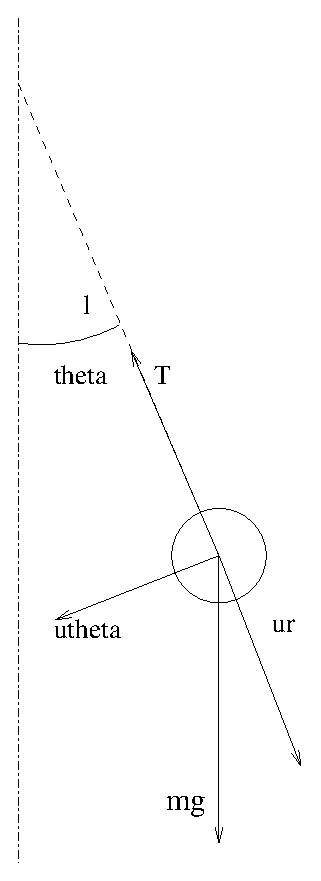
\includegraphics[scale=0.4]{immagini/fisica1/pendolo_forza}
\caption{\index{pendolo}Pendolo semplice}
\end{figure}
\begin{equation*}\ve F=m\ve g+\ve T=m\ve a\end{equation*}
\begin{equation*}\left\{
  \begin{array}{l}
  a_r=-\frac{v^2}{l}=-\omega^2 l\\
  a_\theta=\frac{\ud v}{\ud t}
  \end{array}
  \right.\end{equation*}
\begin{equation*}\left\{
  \begin{array}{l}
  mg\cos\theta-T=-m\omega^2l=-m\frac{v^2}{l}\\
  mg\sin\theta=\frac{\ud v}{\ud t}m
  \end{array}
  \right.\end{equation*}
\begin{equation*}\omega=\frac{v}{l}=\frac{\ud\theta}{\ud t}\end{equation*}
\begin{equation*}|v|=\omega l=l\frac{\ud\theta}{\ud t}\end{equation*}
\begin{equation*}v=-l\frac{\ud\theta}{\ud t}\end{equation*}
\begin{equation*}mg\sin\theta=-ml\frac{\ud^2\theta}{\ud t}\end{equation*}
\begin{equation*}g\sin\theta=-l\frac{\ud^2\theta}{\ud t}\end{equation*}
per piccole oscillazioni\footnote{è il primo sviluppo del polinomio di Taylor}: $\sin\theta\simeq\theta$
\begin{equation*}g\theta=-l\frac{\ud^2\theta}{\ud t}\end{equation*}
$$g\theta=-l\ddot\theta\qquad \theta=A\sin\left(\omega
t+\varphi\right)$$
$$\theta=-\frac{l}{g}\,\ddot\theta\qquad\ddot\theta=-A\omega^2\sin\left(\omega
t+\varphi\right)=-\omega^2\theta$$
\begin{equation*}\theta=-\frac{\ddot\theta}{\omega^2}\qquad \frac{1}{\omega^2}=\frac{l}{g}\qquad\omega^2=\frac{g}{l}\qquad\omega=\sqrt\frac{g}{l}\end{equation*}
\begin{equation*}\theta=A\sin\left(\sqrt\frac{g}{l}\,t+\varphi\right)\end{equation*}
$$2\pi+\sqrt\frac{g}{l}t+\varphi=\sqrt\frac{g}{l}(t+T)+\varphi\qquad
\sqrt\frac{g}{l}T=2\pi\qquad
T=2\pi\sqrt\frac{l}{g}=\frac{2\pi}{\omega}$$

\subsection{\index{forza!variabile!nella velocità}Forze variabili nella velocità}
Su un corpo in caduta agisce la forza di Stokes: $F_s=-\beta v$,
proporzionale alla velocità. $\beta$ dipende dalla viscosità del
mezzo e dalla geometria del corpo.

\begin{equation*}\ve F=m\ve g+\ve F_s=m\ve a\end{equation*}
\begin{equation*}mg-F_s=ma\end{equation*}
\begin{equation*}mg-\beta v=ma=m\frac{\ud v}{\ud t}\end{equation*}
\begin{equation*}mg-\beta v=m\frac{\ud v}{\ud t}\qquad \ud t\left(mg-\beta v\right)=m\ud v\end{equation*}
\begin{equation*}\int_0^t\ud t=\int_{v_0}^v\frac{m}{mg-\beta v}\,\ud v\end{equation*}
$$t=\left[-\frac{m}{\beta}\ln\left(mg-\beta
v\right)\right]_{v_0}^{v}=-\frac{m}{\beta}\left(\ln\left(mg-\beta
v\right)-\ln\left(mg-\beta v_0\right)\right)=$$
\begin{equation*}=-\frac{m}{\beta}\ln\frac{mg-\beta v}{mg-\beta v_0}\qquad-\frac{\beta t}{m}=\ln\frac{mg-\beta v}{mg-\beta v_0}\end{equation*}
\begin{equation*}e^{-\frac{\beta t}{m}}=e^{\ln\frac{mg-\beta v}{mg-\beta v_0}}=\frac{mg-\beta v}{mg-\beta v_0}\end{equation*}
\begin{equation*}(mg-\beta v)=(mg-\beta v_0)e^{-\frac{\beta t}{m}}\end{equation*}
$$v=\frac{mg}{\beta}\left(1-e^{-\frac{\beta
t}{m}}\right)+v_0e^{-\frac{\beta t}{m}}$$

se $t\rightarrow +\infty$ allora $v\rightarrow\frac{mg}{\beta}$

se $\beta\rightarrow 0$ allora $v\rightarrow gt+v_0$
\begin{figure}[htbp]
\centering
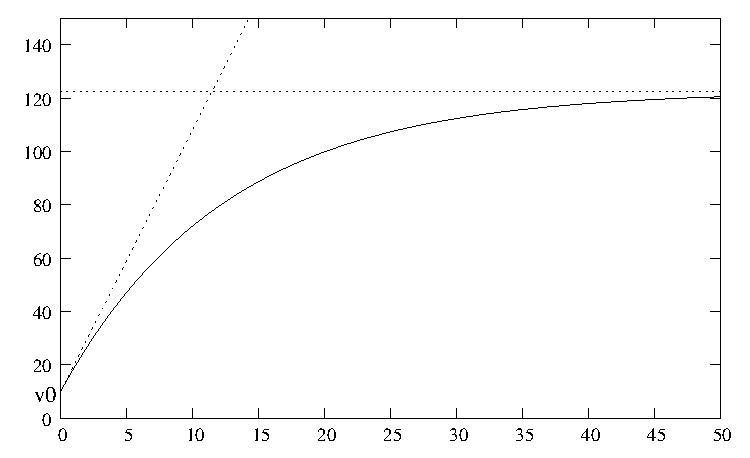
\includegraphics[scale=1]{immagini/fisica1/grafico_forze_nella_velocita}
\caption{Grafico forza variabile nella velocità}
\end{figure}

\section{\index{forza!apparente}Forze apparenti}
Le forze apparenti non sono delle vere forze, sono degli strumenti che consentono di usare la seconda legge delle dinamica anche in sistemi non inerziali. In particolare le forze apparenti non rispettano il terzo principio della dinamica. Siano $O$ e $O'$ due sistemi di riferimento; $O'$ si muova verso destra con accelerazione $\ve a_{O'}$ rispetto ad $O$. $\ve r_{O'}$ il vettore che individua $O'$ rispetto \mbox{ad $O$.}
\begin{figure}[htbp]
   \centering
   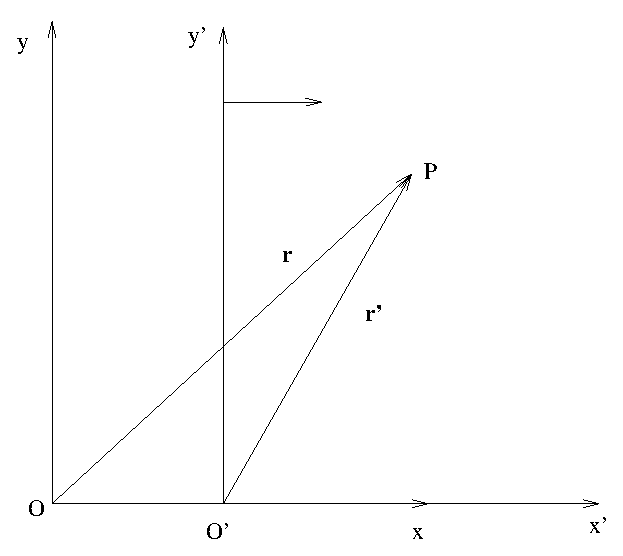
\includegraphics[scale=0.5]{immagini/fisica1/apparenti}
\end{figure}
\begin{equation*}\ve r={\ve r}\,^\prime+\ve r_{O'}\qquad\ve v=\ve v\,'+\ve v_{O'}\qquad\ve a=\ve a\,'+\ve a_{O'}\end{equation*}
\begin{equation*}m\ve a=m\ve a'+m\ve a_{O'}=\ve F\end{equation*}
\begin{equation*}m\ve a'=\ve F-m\ve a_{O'}=\ve F+\ve F_\text{app}\end{equation*}
\begin{equation*}\ve F_\text{app}=-m\ve a_{O'}\end{equation*}
\subsection{Terra}
La Terra non è un sistema inerziale\index{sistema!inerziale}, infatti ruota intorno al Sole e ruota attorno al proprio asse. Consideriamo quest'ultimo moto:
\begin{figure}[htbp]
   \centering
   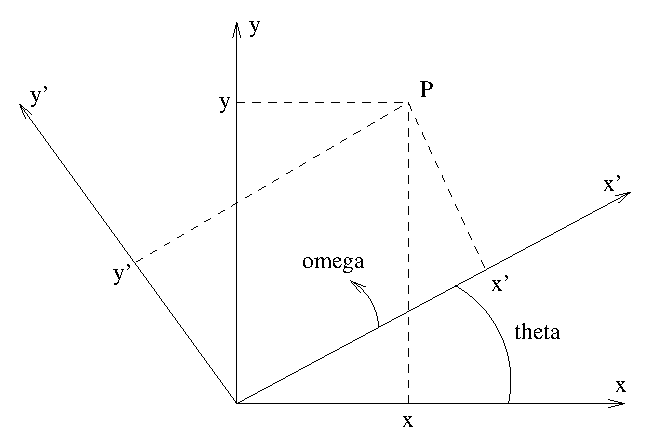
\includegraphics[scale=0.7]{immagini/fisica1/apparenti2}
\end{figure}
\begin{equation*}\left\{\begin{array}{l}
x=x'\cos\theta-y'\sin\theta\\
y=y'\cos\theta+x'\sin\theta
\end{array}\right.\end{equation*}

\begin{equation*}\left\{\begin{array}{l}
x(t)=x'(t)\cos(\omega t)-y'(t)\sin(\omega t)\\
y(t)=y'(t)\cos(\omega t)+x'(t)\sin(\omega t)
\end{array}\right.\end{equation*}

\begin{equation*}v_x=\frac{\ud x}{\ud t}=v'_{x'}\cos\left(\omega t\right)-\omega x'\sin\left(\omega t\right)-v'_{y'}\sin\left(\omega t\right)-\omega y'\cos\left(\omega t\right)\end{equation*}
\begin{align*}
a_x=&\frac{\ud v_x}{\ud t}=a'_{x'}\cos\left(\omega t\right)-\omega v'_{x'}\sin\left(\omega t\right)-\omega v'_{x'}\sin\left(\omega t\right)-\omega^2 x'\cos\left(\omega t\right)-\\
&-a'_{y'}\sin\left(\omega t\right)-\omega v'_{y'}\cos\left(\omega t\right)-\omega v'_{y'}\cos\left(\omega t\right)+\omega^2 y'\sin\left(\omega t\right)\\
=&a'_{x'}\cos\left(\omega t\right)-a'_{y'}\sin\left(\omega t\right)-\omega^2\left[x'\cos\left(\omega t\right)-y'\sin\left(\omega t\right)\right]-\\
&-2\omega\left[v'_{x'}\sin\left(\omega t\right)+v'_{y'}\cos\left(\omega t\right)\right]\\
=&a'_{x}-\omega^2 x-2\omega v'_{y}
\end{align*}
$$\ve \omega\times\ve v'=\left|\begin{array}{ccc}
\ve i&\ve j&\ve k\\
0&0&\omega\\
v'_{x'}&v'_{y'}&v'_{z'}\\
\end{array}
\right|
=-\omega v'_{y'}\ve i+\omega v'_{x'}\ve j$$

$$\left\{\begin{array}{l}
a_x=a'_x-\omega^2 x+2\left(\ve \omega\times\ve v'\right)_x\\
a_y=a'_y-\omega^2 y+2\left(\ve \omega\times\ve v'\right)_y\\
\end{array}\right.$$

\begin{equation*}\ve a=\ve a'-\omega^2 \ve r+2\left(\ve\omega\times\ve v'\right)\end{equation*}
\begin{equation*}m\ve a=m\ve a'-m\omega^2\ve r+2m\left(\ve\omega\times\ve v'\right)=\ve F\end{equation*}
\begin{equation*}ma'=\ve F+\underbrace{m\omega^2\ve r}_\text{forza centrifuga}-\underbrace{2m\left(\ve\omega\times\ve v'\right)}_\text{forza di Coriolis}\end{equation*}\index{Coriolis}\index{forza!centrifuga}\index{forza!di Coriolis}
\begin{equation*}\ve F_\text{cent}=m\omega^2 \ve r\qquad \ve F_\text{Cor}=-2m\left(\ve\omega\times\ve v'\right)\end{equation*}

\begin{Es}[pendolo di Focault\index{Focault}\index{pendolo!di Focault}]
Se mettiamo un pendolo al polo la forza centrifuga sarà nulla perché $r=0$, ma esiste ancora la forza di Coriolis. Sperimentalmente si osserva che il piano di rotazione del pendolo ruota a causa della non inerzialità della Terra.
\end{Es}
\subsection{Trattazione generale}
Consideriamo due sistemi di riferimento in moto rototraslatorio relativo. Siano $\{\ve{e}_i\}_i^3$ e $\{\ve{e}'_i\}_i^3$ i versori dei due sistemi. Ogni vettore di $O$ si scrive come combinazione lineare i cui coefficienti sono le coordinate $\{x_i\}_i^3$:
\begin{equation*}
 \ve{x}=\sum_{i=1}^3 x_i\ve{e}_i
\end{equation*}
sia $x_0$ il vettore posizione di $O'$ visto da $O$:
\begin{equation*}
 \ve{x_0}=\sum_{i=1}^3 {x_0}_i \ve{e}_i
\end{equation*}
nella base del sistema $O'$ il punto individuato da $\ve x$ rispetto al sistema $O$ è individuato dal vettore $\ve{x'}$:
\begin{equation*}
 \ve{x'}=\sum_{i=1}^3 x'_i\ve{e'}_i
\end{equation*}
La relazione che li lega è:
\begin{equation*}
 \ve{x} =  \ve{x_0}+\ve{x'}
\end{equation*}
\begin{equation*}
 \ve{v}=\frac{\ud}{\ud t}\ve{x}=\frac{\ud}{\ud t}\ve{x_0}+\frac{\ud}{\ud t}\ve{x'}=\ve{v_0}+\sum_{i=1}^3\left(\underbrace{\frac{\ud x'_i}{\ud t}\ve{e}'_i}_{\ve{v'}}+x'_i\frac{\ud \ve{e}'}{\ud t}\right)
\end{equation*}
A causa della rotazione il versore del sistema primato ruota, ma il suo modulo non cambia. Dopo un tempo $\ud t$ avrà fatto un angolo $\ud\alpha=\omega\ud t$, quindi per la definizione di angolo $\ud\alpha=\norm{\ud\ve{e'_i}}$, ma allora $\norm{\frac{\ud \ve{e'}_i}{\ud t}} = \omega$. In generale vale:
\begin{equation*}
 \frac{\ud\ve{e'_i}}{\ud t}=\ve\omega\times\ve{e'_i}
\end{equation*}
quindi:
\begin{equation*}
 \ve{v}=\ve{v'}+\ve{v_0}+\ve{\omega}\times\ve{x'}
\end{equation*}
derivando ancora una volta
\begin{align*}
 \ve{a}&=\frac{\ud}{\ud t}\ve{v}=\frac{\ud}{\ud t}\left(\frac{\ud x'_i}{\ud t}\ve{e'_i}\right)+\frac{\ud\ve{v_0}}{\ud t}+\ve\omega\times\frac{\ud\ve{x'}}{\ud t}\\
&=\frac{\ud^2 x'_i}{\ud t^2}\ve{e'_i}+\frac{\ud x'_i}{\ud t}\frac{\ud\ve{e'_i}}{\ud t}+\ve{a_0}+\ve\omega\times\left(\ve{v'}+x'_i\frac{\ud\ve{e'_i}}{\ud t}\right)\\
&=\ve{a'}+\ve\omega\times\ve{v'}+\ve{a_0}+\ve\omega\times\ve{v'}+\ve\omega\times\left(\ve\omega\times\ve{x'}\right)\\
&=\ve{a'}+\ve{a_0}+2\ve\omega\times\ve{v'}+\ve{\omega}(\ve\omega\cdot\ve{x'})-\ve{x'}(\ve\omega\cdot\ve\omega)\\
&=\ve{a'}+\ve{a_0}+2\ve\omega\times\ve{v'}-\omega^2\ve{x'}
\end{align*}
dove nel penultimo passaggio si è usato $\ve A\times(\ve B\times \ve C)=\ve{B}(\ve{A}\cdot\ve{C})-\ve{C}(\ve{A}\cdot\ve{B})$. Moltiplicando per $m$ si ottiene:
\begin{equation}
 m\ve{a'}=\ve F-m\ve{a_0}+m\omega^2\ve x'-2m\ve\omega\times\ve{v'}
\end{equation}







\section{\index{quantità di moto}Quantità di moto}
\begin{Def}[quantità di moto di un punto materiale]
\begin{equation}
\ve{p}:=m\ve{v}
\end{equation}
sinonimi di quantità di moto sono: quantità di modo lineare, momento, momento lineare.
\end{Def}
\begin{equation*}\frac{\ud \ve p}{\ud t}=\frac{\ud\left(m\ve v\right)}{\ud t}=m\ve a=\ve F\end{equation*}
\begin{equation*}\text{Newton disse: }\ve F=\frac{\ud \ve p}{\ud t}\end{equation*}
\subsection{Sistema di $N$ punti}
\begin{Def}[quantità di moto di un sistema di $N$ punti]
La quantità di moto totale di un sistema di $N$ punti è la somma delle quantità di moto.
\begin{equation}
 \ve p=\sum_{I=1}^N\ve p_i=\sum_{i=1}^Nm_i\ve v_i
\end{equation}
\end{Def}
\begin{Teo}
 La variazione della quantità di moto è uguale alle forze esterne
\begin{align*}\frac{\ud \ve p}{\ud t}&=\frac{\ud }{\ud t}\sum^N_{i=1}m_i\ve v_i=\sum_{i=1}^{N}\frac{\ud \left(m\ve v_i\right)}{\ud t}=\sum_{i=1}^{N}m_i\frac{\ud \ve v_i}{\ud t}=\sum_{i=1}^{N}m_i\ve a_i=\\
&=\sum^N_{i=1}\stackrel{\text{Est}}{\ve F_i}+\sum^N_{i=1}\stackrel{\text{Int}}{\ve F_i}=\sum^N_{i=1}\stackrel{\text{Est}}{\ve F_i}\end{align*}
Nell'ultimo passaggio abbiamo usato il terzo principio della dinamica. Si conclude che in un sistema isolato, cioè con
$\sum^N_{i=1}\stackrel{\text{Est}}{\ve F_i}$ vale la legge di
conservazione della quantità di moto: $\ve
p=\overrightarrow\const$.
\end{Teo}
\begin{Es}[carrellini]
Due carrellini di massa $m$ e $M$ si urtano frontalmente con
velocità iniziali $v$ e $V$.
\begin{equation*} P_i= P_f=0\qquad P_f=M V+m v=0\end{equation*}
\begin{equation*}M V=m v\qquad\frac{V}{v}=\frac{m}{M}\end{equation*}
\end{Es}

\begin{Es}[decadimento]
L'uranio decade in questo modo:
\begin{equation*}\mathrm{U}^{238}_{92}\rightarrow \mathrm{Th}^{234}_{90}+\alpha^4_2\end{equation*}
\begin{equation*}\ve p_f=m_{\mathrm{Th}}\ve v_{\mathrm{Th}}+m_\alpha \ve v_\alpha=\ve p_0=0\end{equation*}
\begin{equation*}m_{\mathrm{Th}}v_{\mathrm{Th}}=m_\alpha v_\alpha\qquad v_\alpha=\unita{2\times \power{10}{7}}\metrepersecond\end{equation*}
\begin{equation*}v_{\mathrm{Th}}=\frac{m_\alpha v_\alpha}{m_{\mathrm{Th}}}=\unita{3.4\times
10^5}\metrepersecond\end{equation*}
\end{Es}

\section{\index{centro di massa}Centro di Massa}
\begin{Def}[Centro di massa di $N$ punti]
\begin{equation}\ve r_{CM}=\frac{\sum^N_{i=1}\left(\ve
r_im_i\right)}{\sum^N_{i=1}m_i}=\frac{\sum^N_{i=1}\left(\ve
r_im_i\right)}{M}\end{equation}
\begin{equation*}x_{CM}=\frac{\sum^N_{i=1}\left(x_im_i\right)}{M} \qquad
y_{CM}=\frac{\sum^N_{i=1}\left(y_im_i\right)}{M}\qquad
z_{CM}=\frac{\sum^N_{i=1}\left(z_im_i\right)}{M}\end{equation*}
\end{Def}
\begin{equation*}\ve v_{CM}=\frac{\ud \ve r_{CM}}{\ud t}=\frac{\sum^N_{i=1}\frac{\ud}{\ud t}\left(m_i\ve r_i\right)}{\sum^N_{i=1}m_i}=\frac{\sum^N_{i=1}\left(m_i\ve v_i\right)}{M}\end{equation*}
\begin{equation*}M\ve v_{CM}={\sum^N_{i=1}m_i\ve v_i}=\ve p\end{equation*}
\begin{equation*}\frac{\ud \ve p}{\ud t}=\frac{\ud}{\ud t}M\ve v_{CM}=M\ve a_{CM}=\sum^N_{i=1}\stackrel{\text{Est}}{\ve F_i}\end{equation*}
\begin{Teo}
\begin{equation}M\ve V_{CM}=\ve P \qquad M\ve a_{CM}=\sum \stackrel{\text{Est}}{\ve F_i}\end{equation}
Se il sistema è isolato $\sum \stackrel{\text{Est}}{\ve F}=0$
\begin{equation*}M\ve a_{CM}=0 \Rightarrow \ve a_{CM}=0\end{equation*}
allora il centro di massa si muove di moto rettilineo uniforme.
\end{Teo}

\subsection{Corpo continuo}
\begin{Def}[Centro di massa per un corpo continuo]
\begin{equation}\ve r_{CM}=\frac{\int_V \ve r\,\ud m}{M}\end{equation}
\end{Def}
\begin{Def}[Densità media]
 \begin{equation}\rho =\frac{m}{V}\end{equation}
\end{Def}
\begin{Def}[Densità locale]
 \begin{equation}\rho(x,y,z)=\frac{\ud m}{\ud V}\end{equation}
\end{Def}
\begin{equation*}\ud m=\rho\,\ud V\end{equation*}
\begin{equation*}M=\int_V \ud m=\int_V\rho \,\ud V\end{equation*}
\begin{equation}\ve r_{CM}=\frac{\int_V \ve r \ud V\rho}{M}=\frac{\int_V\rho\ve r\,\ud V}{\int_V \rho \,\ud V}\end{equation}
Se la densità è uguale in tutti i punti il centro di massa è solo un fattore geometrico:
\begin{equation*}\ve r_{CM}=\frac{\int_V\ve r\,\ud V}{V}\end{equation*}

\begin{Es}[semicirconferenza]
\label{es:semicirconferenza}
\begin{figure}[htp]
 \centering
 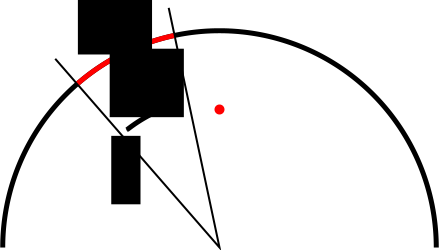
\includegraphics[scale=0.4]{immagini/fisica1/semicerchio}
 \caption{Esempio \ref{es:semicirconferenza}}
\end{figure}

\begin{equation*}x_{CM}=0 \quad\text{per simmetria}\end{equation*}
\begin{equation*}\frac{\ud m}{M}=\frac{\ud s}{\pi r}\qquad \ud s=r\ud\theta\end{equation*}
\begin{equation*}\ud m=\frac{M\ud s}{\pi r}=\frac{Mr\ud\theta}{\pi r}=\frac{M\ud\theta}{\pi}\end{equation*}
\begin{equation*}y=r \sin \theta\end{equation*}
\begin{equation*}y_{CM}=\frac{\int y\ud m}{M}=\frac{r}{\pi}\int_0^\pi \sin\theta \ud \theta=-\frac{r}{\pi}\left[\cos\theta\right]_0^\pi=-\frac{r}{\pi}(-1-1)=\frac{2r}{\pi}\end{equation*}
\end{Es}

\begin{Es}[cerchio bucato]
\label{es:cerchio_bucato}
\begin{figure}[htp]
 \centering
 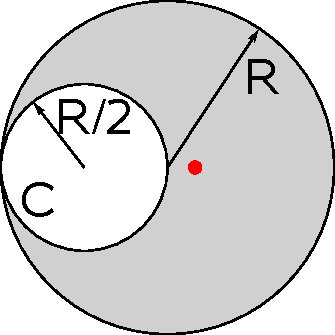
\includegraphics[scale=0.7]{immagini/fisica1/luna}
 \caption{Esempio \ref{es:cerchio_bucato}}
\end{figure}

Luna è il cerchio grande meno il piccolo ($C$) di raggio
$\frac{r}{2} \quad y_{CM}=0$ per simmetria
\begin{equation*}M^C=\rho\pi\left(\frac{r}{2}\right)^2=\rho\pi\left(r^2-\frac{r^2}{4}\right)=\frac{3}{4}\rho\pi r^2\qquad M^{\text{luna}}=\rho\left(\pi r^2-\pi\left(\frac{r}{2}\right)^2\right)\end{equation*}
\begin{equation*}x_{CM}^{\text{pieno}}=0=\frac{x_{CM}^{\text{luna}}+x_{CM}^CM^C}{M^C+M^{\text{luna}}}\end{equation*}
\begin{equation*}0=x_{CM}^{\text{luna}}x_{CM}^C\frac{M^C}{M^{\text{luna}}}=x_{CM}^{\text{luna}}x_{CM}^C\frac{4M^C}{3\rho \pi r^2}=x_{CM}^{\text{luna}}x_{CM}^C\frac{4\rho\pi r^2}{4\cdot 3\rho\pi r^2}=\frac{x_{CM}^{\text{luna}}x_{CM}^C}{3}\end{equation*}
\begin{equation*}x_{CM}^{\text{luna}}=3x_{CM}^C=\frac{R}{6}\end{equation*}
\end{Es}

\subsection{\index{teorema!di Pappo--Guldino}Teorema di Pappo--Guldino}
\begin{Teo}[Pappo--Guldino]
Il volume generato dalla rotazione di una superficie è uguale
all'area della superficie per la distanza percorsa dal centro di
massa durante la rotazione.
\end{Teo}
\begin{Es}[Semicerchio]
Il volume generato dalla rotazione del semicerchio è il volume della
sfera: $\frac{4}{3}\pi r^3$, la distanza percorsa dal centro di
massa è $2\pi y$ con $y$ l'ordinata del centro di massa, la
superficie del semicerchio è $\frac{\pi r^2}{2}$, quindi
\begin{equation*}2\pi y\frac{\pi r^2}{2}=\frac{4}{3}\pi r^3\end{equation*}
\begin{equation*}y=\frac{4}{3\pi}r\end{equation*}
\end{Es}

\section{\index{impulso di una forza}Impulso di una forza}
\begin{align*}
\ve{J}(t_1,t_2)&=\int_{t_1}^{t_2} \ve{F}\, \ud t=\int_{t_1}^{t_2}m\ve a\, \ud t=m\int_{t_1}^{t_2}\frac{d\ve{v}}{\ud t}\,\ud t=m\int_{t_1}^{t_2}\ud \ve{v}\\
&=m\left[\ve v(t_2)-\ve v(t_1)\right]=\ve p_2 - \ve p_1=\Delta \ve p
\end{align*}
\begin{equation*}
\ve J=\int_{t_1}^{t_2}\ve F \ud t=\Delta \ve p
\end{equation*}
Se il sistema è isolato con due corpi si ha:

\begin{equation*}
\Delta \ve p_1=\int_{t_1}^{t_2} \ve F_{1,2}\, \ud t\qquad \Delta \ve p_2=\int_{t_1}^{t_2} \ve F_{2,1}\, \ud t
\end{equation*}
\begin{equation*}
\Delta \ve p_1 + \Delta \ve p_2=\int\left(\ve F_{1,2}+\ve F_{2,1}\right)\ud t=0=\Delta\ve p_{\text{totale}}
\end{equation*}
\begin{equation*}
\ve p_{\text{iniziale}}=\ve p_{\text{finale}}
\end{equation*}
dove si è usato terzo principio della dinamica. La conservazione della quantità di moto vale in tutti i sistemi isolati.

\section{\index{urti}Urti}
Gli urti si classificano in elastici ed anelastici. Gli urti reali sono una via intermedia. Negli urti elastici si conserva tutta l'energia cinetica, agiscono solo forze conservative; durante l'urto l'energia cinetica si trasforma in energia potenziale, per poi tornare completamente energia cinetica. La quantità di moto si conserva sempre in quanto non agiscono forze esterne.

\subsection{\index{urti!elastici}Urti elastici}

\subsubsection{Urti in 1 dimensione}

$$ \left \{
\begin{array}{ll}
   m_1v_{i,1}+m_2v_{i,2}=m_1v_{f,1}+m_2v_{f,2} & v_{1,f}=? \\
   \frac{1}{2}m_1v_{i,1}^2+\frac{1}{2}m_2v_{i,2}^2=\frac{1}{2}m_1v_{f,1}^2+\frac{1}{2}m_2v_{f,2}^2 & v_{2,f}=?
   \end{array}
   \right.$$
\begin{equation*}v_{1,f}=\frac{2m_2}{m_1+m_2}v_{i,2}-v_{i,1}\frac{m_2-m_1}{m_1+m_2}\end{equation*}
\begin{equation*}v_{2,f}=\frac{2m_1}{m_1+m_2}v_{i,1}-v_{i,2}\frac{m_1-m_2}{m_1+m_2}\end{equation*}

\subsubsection{casi limite}
\label{casilimiteurti}
\begin{enumerate}
\item $m_1=m_2$
\begin{equation*}v_{f,1}=v_{i,2}\end{equation*}
\begin{equation*}v_{f,2}=v_{i,1}\end{equation*}
  \begin{itemize}
  \item $v_{i,2}=0$
  \begin{equation*}v_{f,1}=0\end{equation*}
  \begin{equation*}v_{f,2}=v_{i,1}\end{equation*}
  \end{itemize}
\item $m_2\gg m_1$
\begin{equation*}\frac{m_1}{m_2}\simeq 0\end{equation*}
\begin{equation*}v_{f,1}=-v_{i,1}+2v_{i,2}\end{equation*}
\begin{equation*}v_{f,2}=v_{i,2}\end{equation*}
  \begin{itemize}
  \item $v_{i,2}=0$
  \begin{equation*}v_{f,1}=-v_{i,1}\end{equation*}
  \begin{equation*}v_{f,2}=v_{i,2}=0\end{equation*}
  \item $v_{i,1}=0$
  \begin{equation*}v_{f,1}=2v_{i,2}\end{equation*}
  \begin{equation*}v_{f,2}=v_{i,2}\end{equation*}
  \end{itemize}

\end{enumerate}

\subsubsection{Urti in due dimensioni}
Due corpi di massa $m_1$, $m_2$, prima dell'urto velocità $\ve v_{i,2}=0$, $\ve v_{i,1}$, il secondo corpo è fermo, dopo l'urto velocità $\ve v_{f,1}$, $\ve v_{f,2}$.

$$\left\{
\begin{array}{l}
m_1\ve v_{i,1}=m_1\ve v_{f,1}+m_2\ve v_{f,2}\\
\frac{1}{2}m_1 v_{i,1}^2=\frac{1}{2}m_1 v_{f,1}^2+\frac{1}{2}m_2
v_{f,2}^2
\end{array}\right.$$

$$\left\{
\begin{array}{l}
m_1v_{i,1}=m_iv_{f,1}\cos\varphi_1+m_2v_{f,2}\cos\varphi_2\\
0=m_1v_{f,1}\sin\varphi_1-m_2v_{f,2}\sin\varphi_2\\
\frac{1}{2}m_1 v_{i,1}^2=\frac{1}{2}m_1 v_{f,1}^2+\frac{1}{2}m_2
v_{f,2}^2
\end{array}\right.$$
Il sistema è formato da 3 equazioni, ma da 4 incognite
($\varphi_1, \varphi_2, v_{f,1}, v_{f,2}$), ha $\infty^1$
soluzioni.

Nel caso particolare di $m_1=m_2$ si ha:
$$\frac{1}{2}m v_{i,1}^2=\frac{1}{2}m
v_{f,1}^2+\frac{1}{2}m v_{f,2}^2$$
$$\left\{
\begin{array}{l}
v_{i,1}^2=v_{f,1}^2+v_{f,2}^2\\
m^2v_{i,1}^2=m^2v_{f,1}^2+m^2v_{f,2}^2+2m^2v_{1,f}v_{2,f}\cos\alpha
\end{array}
\right.$$

$$\left\{
\begin{array}{l}
v_{i,1}^2=v_{f,1}^2+v_{f,2}^2\\
v_{i,1}^2=v_{f,1}^2+v_{f,2}^2+2v_{1,f}v_{2,f}\cos\alpha
\end{array}
\right.$$

quindi $\cos \alpha=0\quad\Rightarrow\quad\alpha=\unita{90}\degree$, oppure $v_{1,f}=0$ e $v_{2,f}=v_{1,i}$

\subsection{\index{urti!anelastici}Urti completamente anelastici}

Negli urti anelastici il sistema perde la massima energia cinetica possibile, che non è tutta
in quanto se il sistema perdesse tutta l'energia cinetica violerebbe la conservazione
della quantità di moto. Si dimostra che questo caso è quello in cui dopo l'urto i due corpi
rimangono attaccati.

\begin{Es}[pendolo balistico{\index{pendolo!balistico}}]
Un proiettile di massa $m$, velocità $v$ urta un pendolo balistico di massa $M>m$ e velocità $V=0$. Prima dell'urto la quantità di moto totale del sistema è $mv$, dopo $(M+m)V$.
\begin{equation*}mv=(M+m)V\end{equation*}
\begin{equation*}V=\frac{mv}{M+v}\end{equation*}
Dopo l'urto il pendolo balistico, con il proiettile incorporato oscilla come un pendolo, l'energia meccanica si conserva, quindi $K_A=U(B)$


\begin{equation*}\frac{1}{2}(m+M)V^2=(m+M)gh\end{equation*}
\begin{equation*}\frac{1}{2}\left(\frac{mv}{M+m}\right)^2=(m+M)gh\end{equation*}
\begin{equation*}\frac{1}{2}\frac{m^2v^2}{M+m}=(m+M)gh\end{equation*}
\begin{equation*}v^2=\frac{(m+M)gh\cdot 2(m+M)}{m^2}=\frac{2(m+M)^2gh}{m^2}\end{equation*}
\begin{equation*}v=\frac{m+M}{m}\sqrt{2gh}\end{equation*}
Consideriamo un sistema di riferimento $\ast$ inerziale rispetto
al CM con la stessa velocità del CM.

\begin{equation*}\ve P^\ast_{\text{prima}}=(m+M)\ve V_{\text{CM}}^\ast=0\end{equation*}
$$\ve P^\ast_{\text{dopo}}=0\quad\text{sono attaccati}\quad \ve
v=0$$ Quindi tutta l'energia cinetica è persa.
\end{Es}
\section{\index{momento!d'inerzia}Momento d'inerzia}
Corpo rigido(CR): presi due punti qualsiasi la loro distanza
rimane inalterata. Servono tre punti, quindi 9 coordinate, ma le
distanze rimangono fisse nel tempo, quindi il corpo ha 6 gradi di
libertà. Per descrivere il moto di un corpo bisogna dare 6
coordinate in funzione del tempo. Se fissiamo un asse di rotazione
si ha un solo grado di libertà. In questo caso si ha una rotazione
intorno ad un asse fisso. Ogni punto del CR descrive una
circonferenza. $\theta$ è comune a tutti, quindi anche $\omega$ e
$\alpha$
\begin{equation*}\ud s_i=\ud \theta r_i\end{equation*}
\begin{equation*}v_i=r_i\omega \qquad a_t=\frac{\ud v_i}{\ud t}=\alpha r_i\end{equation*}
\begin{equation*}K=\sum_i\frac{1}{2}m_iv_i^2\end{equation*}
\begin{equation*}K=\sum_i\frac{1}{2}m_i\omega^2r_i^2=\frac{1}{2}\omega^2\left(\sum_im_ir_i^2\right)=\frac{1}{2}I\omega^2\end{equation*}
\begin{equation*}I=\text{momento d'inerzia}=\sum_{i=1}^N m_ir_i^2\end{equation*}
\begin{equation*}\text{Nel caso di corpo continuo} \sum_{i=1}^\infty \ud m_ir_i^2=\int_V  r^2\,\ud m\end{equation*}
Essendo $\ve r$ relativo a un punto $O$ allora anche $I$ sarà relativo ad $O$. Bisogna sempre specificare rispetto quale punto si calcola $I$.

\subsection{Calcolo Momenti di Inerzia}

\begin{minipage}[c]{\textwidth}
\subsubsection{Barra Sottile per l'estremo}

   \centering
   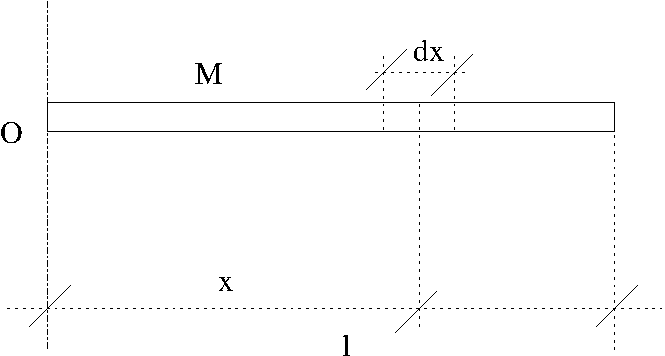
\includegraphics[scale=0.4]{immagini/fisica1/sbarra_sottile1}

\begin{equation*}\frac{\ud m}{M}=\frac{\ud x}{l}\end{equation*}
\begin{equation*}I_0=\int_0^l\frac{M}{l}\ud x x^2=\frac{M}{l}\left[\frac{x^3}{3}\right]_0^l=\frac{M}{l}\frac{l^3}{3}=\frac{M}{3}l^2\end{equation*}
\end{minipage}

\subsubsection{Barra sottile per il centro di massa}
$$I_c=\int_{-l/2}^{l/2}\frac{M}{l}\ud x
x^2=\frac{M}{l}\int_{-l/2}^{l/2}x^2 \ud
x=\frac{M}{3l}\left(\frac{l^3}{8}+\frac{l^3}{8}\right)=\frac{M}{12}l^2$$

\subsubsection{Disco}


\begin{figure}[htbp]
   \centering
   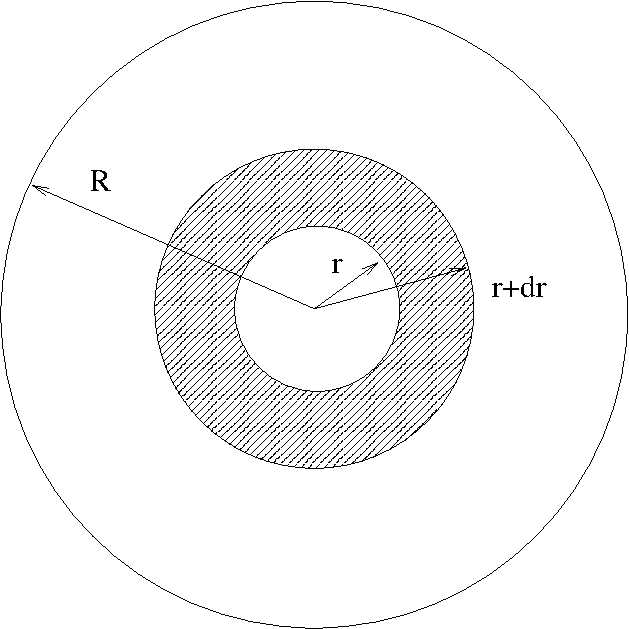
\includegraphics[scale=0.3]{immagini/fisica1/disco}
\end{figure}

\begin{equation*}\frac{\ud m}{M}=\frac{2\pi r\ud r}{\pi R^2}\end{equation*}
\begin{equation*}\ud m=M\frac{2\ud r}{R^2}r\end{equation*}
$$I_O=\int_O^R\frac{M}{R^2}2\ud r r^3=\frac{2M}{R^2}\int_O^R r^3
\ud r=\frac{2M}{R^2}\cdot\frac{R^4}{4}=\frac{1}{2}MR^2$$

\subsubsection{Sfera omogenea}

\begin{minipage}[]{\textwidth}
Dividiamo la sfera in tanti dischetti:
\vspace{0.7cm}

   \centering
   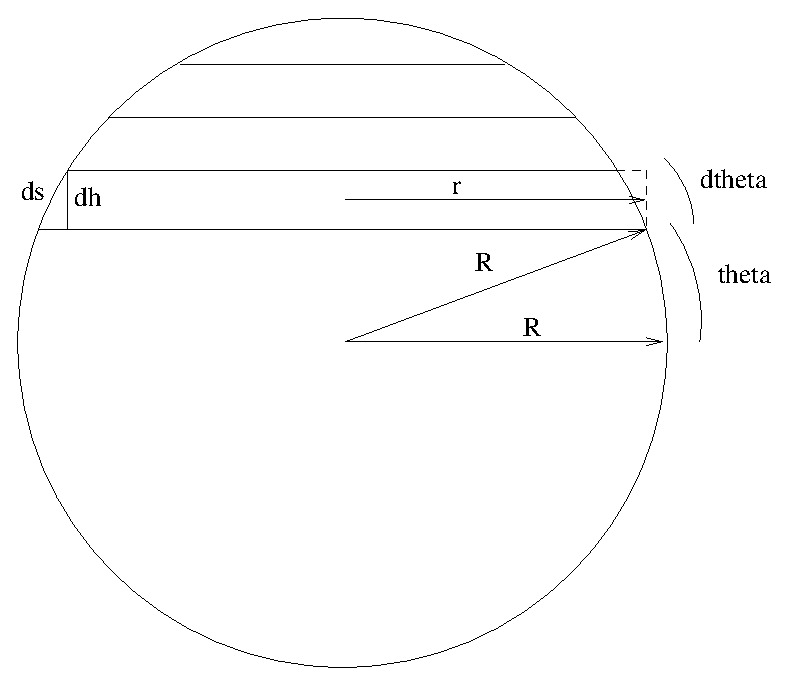
\includegraphics[scale=0.45]{immagini/fisica1/sfera_omogenea1}

\end{minipage}
\begin{equation*}r=R\cos\theta\quad \ud s=R\ud\theta\quad \ud h=\ud s\cos\theta=R\ud\theta\cos\theta\end{equation*}
\begin{equation*}\ud m=\rho\ud V=\rho\pi r^2\ud h=\rho\pi R^2\cos^2\theta R\cos\theta\ud\theta=R^3\rho\pi\cos^3\theta\ud\theta\end{equation*}
\begin{equation*}I_\text{dischetto}=\ud I=\frac{1}{2}\ud m r^2=\frac{1}{2}\rho\pi R^3\cos^3\theta\ud\theta R^2\cos^2\theta=\frac{1}{2}\rho\pi R^5\cos^5\theta\ud\theta\end{equation*}
\begin{equation*}m=\rho\frac{4}{3}\pi R^3\end{equation*}
\begin{equation*}I_\text{sfera}=2\int_0^\frac{\pi}{2}\ud I=\frac{3}{4}mR^2\int_0^\frac{\pi}{2}\cos^5\theta\ud\theta=\frac{2}{5}mR^2\end{equation*}

\subsection{\index{teorema!di Steiner}\index{teorema!degli assi paralleli}Teorema di Steiner o degli assi paralleli}
\begin{Teo}[Steiner o degli assi paralleli]Sia $d$ la distanza da un asse di rotazione $I_0$ parallelo all'asse $I_{CM}$ passante per il centro di massa. Allora:
\begin{equation*}I_0=d^2M+I_{CM}\end{equation*}
\end{Teo}
\begin{figure}[htbp]
   \centering
   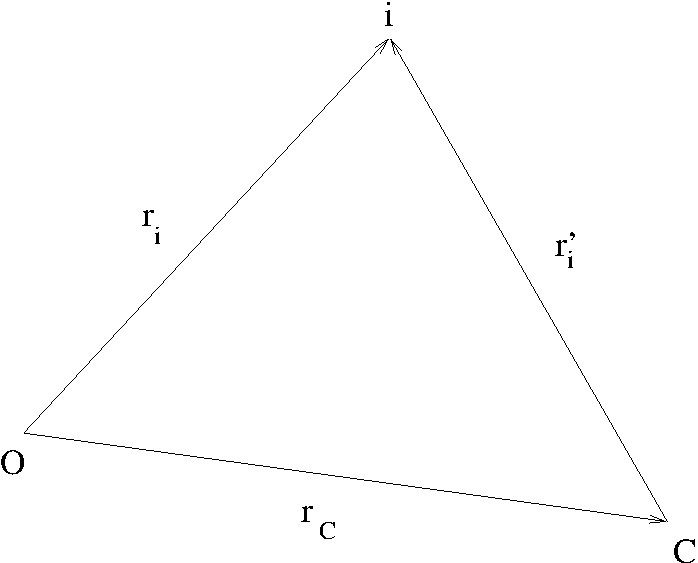
\includegraphics[scale=0.45]{immagini/fisica1/steiner}
\end{figure}
\begin{equation*}\ve r_i=\ve r_C+\ve r_i\,'\end{equation*}
$$\ve r_i\cdot\ve r_i=r_i^2=\left(\ve
r_C+r_i\,'\right)\cdot\left(\ve r_C+\ve r_i\,'\right)\Rightarrow
r_i^2=r_C^2+r_i\,'^2+2\ve r_C\cdot\ve r_i\,'$$
\begin{align*}
I_0&=\sum m_ir_i^2=\sum r_C^2m_i+\sum r_i\,'^2m_i+\sum m_i
\cdot 2\ve r_C\cdot \ve r_i\,'\\
&=r_C^2\sum m_i+I_C+2\ve
r_C\cdot\sum m_i\ve r_i\,'=d^2M+I_{C}+2\ve r_C\cdot\sum m_i\cdot
\ve r_i\,'\end{align*}
Per ipotesi $C$ è il $CM$ del sistema
$$I_0=d^2 M+I_{CM}+2\ve r_i\frac{\sum m_i\ve r_i\,'}{M}\cdot
M=d^2M+I_{CM}+2\ve r_i\cdot \ve r\,_{CM}^{CM} M=d^2M+I_{CM}$$
Ma $Md^2>0$ quindi $I_{CM}$ è il momento minimo possibile.
\begin{Es}
Il momento d'inerzia di una circonferenza rispetto al centro di massa è \mbox{$I_{CM}=\frac{1}{2}MR^2$}, per un estremo è:
\begin{equation*}I_0=I_{CM}+MR^2=\frac{1}{2}MR^2+MR^2=\frac{3}{2}MR^2>I_{CM}\end{equation*}
\end{Es}
\section{\index{momento!di una forza}Momento di una forza}
$$\text{Rispetto al polo $0$ fisso:}\quad\ve{\tau}_0=\ve r \times \ve F=\left |
\begin{array}{lll}
\ve i & \ve j & \ve k\\
x & y & z\\
F_x & F_y &F_z\\
\end{array}
\right|$$
\begin{equation*}\delta L=\ud K\qquad \ud \ve s=\ve r\ud \theta\end{equation*}
\begin{equation*}\delta L=F\ud s\cos \phi=Fr\ud\theta\cos\phi\end{equation*}
\begin{equation*}K=\frac{1}{2}I\omega^2\qquad\ud K=I\omega\ud\omega\end{equation*}
\begin{equation*}Fr\ud\theta\cos\phi=I\omega\ud\omega\end{equation*}
$$Fr\frac{\ud\theta}{\ud t}\cos\phi=I\omega\frac{\ud\omega}{\ud
t}$$
\begin{equation*}Fr\omega\cos\phi=I\omega\alpha\end{equation*}
\begin{equation*}Fr\cos\phi=I\alpha\end{equation*}
\begin{equation*}Fr\sin\beta=I\alpha\end{equation*}
\begin{equation*}\ve\tau=I\ve\alpha\qquad\text{analoga a $\ve F=m\ve a$}\end{equation*}
\section[\index{momento!angolare}\index{momento!della quantità di moto}Momento angolare o della quantità di moto]{Momento angolare\\ o momento della quantità di moto}
\begin{equation*}\ve l_0=\ve r\times m\ve v\qquad\text{rispetto al polo $0$ fisso.}\end{equation*}
\begin{align*}
\frac{\ud \ve l_0}{\ud t}&=\frac{\ud}{\ud t}\left(\ve r\times m\ve v\right)= \frac{\ud\ve r}{\ud t}\times m\ve v+\ve r\times\frac{\ud m\ve v}{\ud t}\\
&=\ve v\times m\ve v+\ve r \times m\ve a=\ve r\times m\ve a=\ve r\times\ve F=\ve \tau_0
\end{align*}
$$\frac{\ud\ve l_0}{\ud t}=\ve \tau_0\qquad\text{analoga
a}\qquad\frac{\ud \ve p}{\ud t}=\ve F$$
\subsection{Sistema di N punti}
\begin{equation*}\ve L_0=\sum_{i=1}^N \ve l_{0_i}\end{equation*}
\begin{align*}\frac{\ud \ve L_0}{\ud t}&=\sum_{i=1}^{N}\frac{\ud \ve l_{0_i}}{\ud
t}=\sum_{i=1}^{N}\frac{\ud}{\ud t}\left(\ve r_i \times \ve
v_i\right)=\sum_{i=1}^{N}\ve v_i\times m_i \ve v_i+\ve
r_i\times m_i\ve a_i\\
&=\sum_{i=1}^{N}\ve r_i\times m_i\ve
a_i=\sum_{i=1}^{N}\ve r_i\times\ve F_i\\
&=\sum_{i=1}^{N}\ve
r_i\times\stackrel{\text{Int}}{\ve F_i}+\sum_{i=1}^{N}\ve
r_i\times\stackrel{\text{Est}}{\ve F_i}=\sum_{i=1}^{N}\ve
r_i\times \stackrel{\text{Est}}{\ve
F_i}=\sum_{i=1}^{N}\stackrel{\text{Est}}{\ve \tau_0}\end{align*}
\subsubsection{Dimostrazione $\stackrel{\text{Int}}{\ve\tau_0}=0$}
\begin{equation*}\ve F_{1,2}=-\ve F_{2,1}\end{equation*}
\begin{equation*}\ve r_1\times \ve F_{1,2}+\ve r_2\times\ve F_{2,1}=\ve r_1\times \ve F_{1,2}-\ve r_2\times\ve F_{1,2}=\left(\ve r_i-\ve r_2\right)\times\ve F_{1,2}=0\end{equation*}
perché $\left(\ve r_1-\ve r_2\right)\parallel \ve F_{1,2}$
\subsection{Conservazione del momento angolare}
Se il sistema è isolato si ha: $\stackrel{\text{Est}}{\ve
F}=0\Rightarrow \stackrel{\text{Est}}{\ve \tau}=0$
$$\frac{\ud \ve L_0}{\ud t}=\ve \tau_0=0\qquad \ve
L_0=\overrightarrow{\const}$$ e quindi
$I\omega={\const}$. Tutto ciò per la simmetria per
rotazioni.
\subsection{Rotazione intorno a $O'$ mobile}
\begin{equation*}\ve r_i=\ve r_{O'}+\ve r_i\,'\qquad \ve r_i\,'=\ve r_i-\ve r_{O'}\end{equation*}
$$L_{O'}=\sum\ve r_i\,'\times m\ve v_i=\sum(\ve r_i-\ve
r_{O'})\times m\ve v_i$$
\begin{align*}
\frac{\ud L_{O'}}{\ud t}&=\sum(v_i-v_{O'})\times m\ve v_i+r_i\,' m\ve a_i=-\sum\ve v_{O'}\times m_i\ve v_i+\sum\ve r_i\,'\times\ve F_i\\
&=\ve v_{O'}\times\sum m_i\ve v_i+\ve \tau_{O'}=-\ve
v_{O'}\times\ve P+\stackrel{\text{Est}}{\tau_{O'}}
\end{align*}
\begin{equation*}\frac{\ud L_O}{\ud t}=-\ve v_{O'}\times\ve P+\stackrel{\text{Est}}{\tau_{O'}}\end{equation*}

se $v_{O'}=0$ allora $-v_{O'}\times\ve P=0$

se $O'=CM$ allora $M\ve V_{CM}=\ve p\Rightarrow\ve
v_{CM}\parallel\ve P\Rightarrow -\ve v_O\times\ve P=0$

\subsection{Rotazione intorno ad un asse}
\begin{equation*}\ve l_i=\ve r_i\times m_i\ve v_i\end{equation*}
\begin{equation*}l_{i_z}=|\ve l_i|\sin\theta_i\end{equation*}
$$|\ve l_i|=r_im_iv_i\qquad l_{i_z}=r_im_iv_i\sin\theta_i\qquad
\omega d_i=v_i$$
\begin{equation*}l_{i_z}=m_id_i\omega d_i=md_i^2\omega\end{equation*}
\begin{equation*}l_{i_z}=m_i\omega R_i^2\end{equation*}
\begin{equation*}L_z=\sum l_{i_z}=\sum(m_id_i^2)\omega=I\omega\end{equation*}
\begin{equation*}L_z=I\omega\end{equation*}
$$\frac{\ud l_{i_z}}{\ud t}=I\frac{\ud \omega}{\ud
t}=I\alpha\qquad \stackrel{\text{Est}}{\tau_{z}}=I\alpha$$
\subsection{Corpo simmetrico rispetto all'asse di rotazione}
\begin{equation*}\ve l_i+\ve l_{i'}=\alpha\ve k\end{equation*}
\begin{equation*}L=I\omega=L_z\end{equation*}


\section{Analogia tra grandezze lineari e \mbox{rotazionali}}
\begin{small}
\begin{tabular}{p{4.0cm}p{2.45cm}p{4.0cm}p{2.38cm}}
\hline
Grandezze lineari &&Grandezze rotazionali&\\
\hline
velocità&$\ve v=\ud \ve r/\ud t$ & velocità angolare&$\ve\omega=\ud \phi/\ud t$\\
Accelerazione&$\ve a=\ud \ve v/\ud t$&Accelerazione
angolare&$\ve\alpha=\ud \ve\omega/\ud t$\\
Massa&$m$&Momento d'inerzia&$I=\sum mr^2$\\
Forza&$\ve F$&Momento di una forza&$\ve \tau=\ve r\times \ve F$\\
Seconda legge di Newton&$\sum \stackrel{\text{Est}}{\ve F}=m\ve
a$& Seconda legge di Newton per moto rotatori con asse
fisso&$\sum\stackrel{\text{Est}}{\ve \tau_z}=I\alpha_z$\\
Condizione di equilibrio&$\sum\stackrel{\text{Est}}{\ve
F}=0$&Condizione di equilibrio&$\sum\stackrel{\text{Est}}{\ve
\tau}=0$\\
quantità di moto di una particella&$\ve p=m\ve v$&Momento
angolare di una particella&$\ve l=\ve r\times \ve p$\\
quantità di moto di un sistema di particelle&$\ve P=M\ve
v_{CM}$&Momento angolare di un sistema di particelle&$\ve
L=I\omega$\\
Forma generale della seconda legge di
Newton&$\sum\stackrel{\text{Est}}{\ve F}=\ud \ve P/\ud t$&Forma
generale della seconda legge di Newton per i moti
rotatori&$\sum\stackrel{\text{Est}}{\ve \tau}=\ud \ve L/\ud t$\\
Conservazione della quantità di moto di un sistema di particelle
per il quale $\sum\stackrel{\text{Est}}{\ve F}=0$&$\ve P=\sum
\ve p_n=$ \mbox{$=\overrightarrow\const$}&Conservazione del momento angolare di un sistema di particelle per il quale $\sum\stackrel{\text{Est}}{\ve \tau}=0$&$\ve L=\sum \ve l_n=$ \mbox{$=\overrightarrow\const$}\\
\hline
\end{tabular}
\end{small}

\chapter{Lavoro ed energia}
\section{\index{lavoro}Lavoro definizione}
Il lavoro è una grandezza scalare.
\begin{Def}[lavoro]
Definiamo lavoro $L$ fatto dalla $\ve F$ sul punto $P$ lungo il percorso $\Gamma$ l'integrale su $\Gamma$ della forma differenziale $\ve F\cdot\ud\ve s$:
\begin{equation}
L=\int_\Gamma\ve F\cdot\ud \ve s
\end{equation}
\end{Def}
Distinguiamo i seguenti casi particolari:
\begin {enumerate}
\item[a)]  Forza costante e parallela allo spostamento
\begin{equation*}L=Fs\end{equation*}

\item[b)] Forza costante non parallela allo spostamento
\begin{equation*}L=Fs\cos\alpha=\ve F \cdot \ve s\end{equation*}

\item[c)] Forza parallela ma variabile
\begin{equation*}L=\int_A^B F(x)\,\ud x\end{equation*}

\item[d)] Forza variabile, traiettoria qualsiasi (caso generale)
\begin{equation*}\delta L=\ve F\cdot\ud \ve s\end{equation*}
\begin{equation*}{L=\int_A^B\delta L \quad \text{curvilineo}}\end{equation*}
\end{enumerate}
\begin{Es}[attrito costante su traiettoria semicircolare]
\begin{equation*}F_A=\mu N=\mu mg\quad \delta L=\ve F_A\cdot\ud \ve s=-\mu mg\ud s\end{equation*}
$$L=\int_A^B \delta L=\int_A^B -\mu mg\ud s=-\mu mg\int_A^B\ud
s=-\mu mg\pi R$$
\end{Es}
\subsection{Lavoro nei moti rotatori}
Corpo rigido ruotante attorno ad un asse. $\ud s$ lo spostamento
infinitesimale corrispondete a $\ud \theta$, $\phi$ l'angolo
compreso tra la forza e il vettore $\ve r$:

$$\delta L=(F\sin \phi)\ud s=(F \sin \phi)(r
\ud\theta)=(rF\sin\phi)\ud \theta=\tau_z\ud\theta$$
\begin{equation*}L=\int_{\theta_i}^{\theta_f}\tau_z\ud\theta\end{equation*}
Se durante la rotazione il momento torcente resta costante, il
lavoro svolto da questo momento torcente è:
\begin{equation*}L=\tau_z\theta\end{equation*}
\section{\index{potenza}Potenza}
\begin{Def}[potenza]
 \begin{equation*}P=\frac{\ud L}{\ud t}\end{equation*}
\end{Def}
La potenza si misura nel SI in $\joule\per\second$ cioè \watt(watt).
$$P=\frac{\ud L}{\ud t}=\frac{\ve F\cdot\ud \ve s}{\ud t}=\ve F\cdot\frac{\ud \ve s}{\ud
t}=\ve F\cdot \ve v$$
\subsection{Potenza nei moti rotatori}
$$P=\frac{\ud L}{\ud t}=\frac{\tau_z\ud\theta}{\ud
t}=\tau_z\omega$$

\section[Energia Cinetica]{\index{energia!cinetica}Energia Cinetica}
\begin{Def}[energia cinetica]
\begin{equation*}K=\frac{1}{2}mv^2\end{equation*}
\end{Def}
A volte indicata con $T$.
\subsection{Teorema lavoro--energia\index{teorema!lavoro--energia}}
\begin{equation*}\delta L=\ve F\cdot\ud \ve s=\ve F\cdot\frac{\ud \ve s}{\ud t}\ud t=\ve F\cdot\ve v\ud t=m\ve a\cdot\ve v\ud t=m\frac{\ud \ve v}{\ud t}\cdot\ve v\ud t=m\ve v\ud \ve v=mv\ud v\end{equation*}
\begin{equation*}\ud K=\ud \left(\frac{1}{2}mv^2\right)=\ud \left(\frac{1}{2}mvv\right)=\frac{1}{2}m\left(\ud vv+v\ud v\right)=\frac{1}{2}m2v\ud v=mv\ud v\end{equation*}
\begin{equation*}\delta L=\ud K\qquad\int_A^B\delta L=\int_A^B \ud K\end{equation*}
\begin{Teo}[lavoro--energia]
\begin{equation*}L=K_B-K_A=\Delta K\end{equation*}
\end{Teo}
Il lavoro è allora la variazione dell'energia cinetica


\section{Complementi -- Funzioni in due variabili}

\begin{equation*}z=f(x,y)\end{equation*}
\index{derivata!parziale}derivata parziale:
\begin{equation*}\frac{\partial z}{\partial x}=\frac{\partial f}{\partial x}=\frac{\ud f}{\ud x}\ \text{considerando $y$ costante}\end{equation*}
derivate seconde parziali:
$$
\frac{\partial^2 z}{\partial x^2}\qquad \frac{\partial^2
z}{\partial y^2}\qquad \frac{\partial^2 z}{\partial x\partial
y}\qquad\frac{\partial^2 z}{\partial y\partial x}$$
\begin{Teo}[Shwartz]
Sotto opportune ipotesi\footnote{Sia $\Omega\subseteq\field{R}^n$ aperto e sia $f:\Omega\to\mathbb{R}$. Supponiamo che le derivate parziali miste $\frac{\partial^2 f}{\partial x_k\partial x_j}$, $\frac{\partial^2 f}{\partial x_j\partial x_k}$ esistano in un intorno $a\in\Omega$ e siano continue in $a$. Allora esse sono uguali in $a$} le derivate seconde parziali incrociate sono uguali:
\begin{equation*}\frac{\partial^2 z}{\partial x\partial y}=\frac{\partial^2 z}{\partial y\partial x}\end{equation*}
\end{Teo}
\begin{Def}[\index{forma differenziale! lineare}Forma differenziale lineare]
\begin{equation*}\delta G=H(x,y)\ud x+K(x,y)\ud y\end{equation*}
\end{Def}
\begin{Def}[\index{differenziale!totale}\index{differenziale!esatto}Differenziale totale o esatto]
\begin{equation*}\ud z=\frac{\partial z}{\partial x}\,\ud x+\frac{\partial z}{\partial y}\,\ud y\end{equation*}
\end{Def}
è una forma differenziale lineare.
\begin{Teo}
 Una forma differenziale lineare è un differenziale esatto se e
solo se:
\begin{equation*}\frac{\partial H}{\partial y}=\frac{\partial K}{\partial x}\end{equation*}
\end{Teo}
Il lavoro elementare è una forma differenziale lineare:
\begin{equation*}\delta L=\ve F\cdot \ud \ve s=F_x\ud x+F_y\ud y=F_x(x,y)\ud x+F_y(x,y)\ud y\end{equation*}
\begin{equation*}L_A^B=\int_A^B\delta L=\int_A^B F_x(x,y)\ud x+F_y(x,y)\ud y\end{equation*}
\begin{equation*}\text{se } \frac{\partial F_x}{\partial y}=\frac{\partial F_y}{\partial x} \Rightarrow \delta L= \text{differenziale totale}\end{equation*}
\begin{equation*}\delta L=\ud L=\ud V\end{equation*}
Allora si avrà, qualunque sia il cammino percorso:
\begin{equation*}L_A^B=\int_A^B \ud V=V(B)-V(A)\end{equation*}
e la \index{forza!conservativa}forza si dice conservativa.
\begin{equation*}F_x(x,y)=\frac{\partial V}{\partial x}\qquad F_y(x,y)=\frac{\partial V}{\partial y}\end{equation*}
In termini sintetici:
 \begin{equation*}\ve F=\ve\nabla V\end{equation*}
 Per dettagli sull'operatore
gradiente vedi sezione \ref{gradiente} a pagina
\pageref{gradiente}.

\subsection{\index{circuitazione!di una forza}Circuitazione di una forza}
\`E il lavoro calcolato su una traiettoria chiusa
\begin{equation*}\oint \ve F\cdot\ud \ve s=0 \quad \text{se la forza è conservativa}\end{equation*}

\section{\index{energia!potenziale}Energia Potenziale}
\begin{equation*}U=-V\end{equation*}
\begin{equation*}L_A^B=U(A)-U(B)=-\Delta U\end{equation*}
Considerando l'energia potenziale in $0$ nulla si ha\footnote{c'è molta confusione sulle notazioni, frequentemente quello che qui è chiamato $V$ è chiamato $U$ e l'energia potenziale $U$ è chiamata $V$}:
\begin{equation*}L_0^P=U(0)-U(P)=0-U(P)\end{equation*}
\begin{equation*}U(P)=-L_0^P=-\int_0^P \ve{F}\cdot\ud \ve{s}\end{equation*}
\begin{equation*}\ve F=-\ve\nabla U\end{equation*}

\subsection{\index{conservazione! dell'energia meccanica}Conservazione dell'energia meccanica}
\begin{Def}[Energia meccanica]
 L'energia meccanica è la somma di energia cinetica e energia potenziale.
\end{Def}
\begin{Teo}[Conservazione energia meccanica]
Considerando solo forze conservative:
\begin{equation*}L_A^B=U_A-U_B\qquad L_A^B=K_B-K_A\end{equation*}
\begin{equation*}U_A+K_A=U_B+K_B\end{equation*}
\begin{equation*}U(P)+K=E=\const\end{equation*}
\end{Teo}
\index{forza!conservativa}Per verificare se una forza è conservativa:

\begin{enumerate}
\item$$\frac {\partial F_x}{\partial y}=\frac {\partial
F_y}{\partial x}$$ se sì allora è conservativa, se no non lo è

\item\begin{equation*}U(0)=0 \qquad L_0^P=U(0)-U(P)=-U(P)\end{equation*}
\begin{equation*}U(P)=-\int_0^P \ve F\cdot\ud \ve s\end{equation*}

\item Verifica
\begin{equation*}\frac {\partial U}{\partial x}=-F_x \qquad \frac{\partial U}{\partial y}=-F_y\end{equation*}
\end{enumerate}
\begin{Es}[Forza peso $F_x=0 \quad F_y=mg$]
\begin{enumerate}
\item $\frac {\partial F_x}{\partial y}=0=\frac {\partial
F_y}{\partial x}$

\item $U(P)=-\int_0^P  \ve F\, \ud \ve s=\int_0^P F_x\, \ud x+F_y\, \ud
y=\int_0^P mg \, \ud y = mgy$

\item $\frac {\partial U}{\partial x}=0=-F_x\quad \frac {\partial
U}{\partial y}=mg=-F_y$
\end{enumerate}
\end{Es}
\begin{Es}[Forza elastica $F_x=-kx \quad F_y=-ky$]
\begin{enumerate}
\item$\frac {\partial F_x}{\partial y}=0=\frac {\partial
F_y}{\partial x}$

\item$U(P)=-\int_0^P \ve F\, \ud \ve s=\left(\int_0^P F_x\, \ud x+\int_0^P
F_y\, \ud y \right)=\frac
{1}{2}kx^2+\frac{1}{2}ky^2=\frac{1}{2}kr^2$

\item$\frac{\partial U}{\partial x}=kx=-F_x \quad \frac{\partial
U}{\partial y}=ky=-F_y$
\end{enumerate}
\end{Es}
\begin{Es}[Forza gravitazionale $ \ve{F}=-G\frac{Mm}{{r^3}}\ve r \quad
r=\sqrt{x^2+y^2}$]

\begin{enumerate}

\item
\begin{equation*}F_x=\frac {-GMm}{r^3}x=-GMmx(x^2+y^2)^{-\frac{3}{2}}\end{equation*}
\begin{equation*}F_y=\frac {-GMm}{r^3}y=-GMmy(x^2+y^2)^{-\frac{3}{2}}\end{equation*}
\begin{equation*}\frac{\partial F_x}{\partial y}=GmMx\frac {3}{2}(x^2+y^2)^{-\frac{5}{2}}2y=\frac{\partial F_y}{\partial x}=GmMy\frac {3}{2}(x^2+y^2)^{-\frac{5}{2}}2x \end{equation*}
\begin{equation*}\frac{\partial F_x}{\partial y}=\frac{\partial F_y}{\partial x}\quad \Rightarrow\quad \text{è conservativa}\end{equation*}

\item\begin{equation*}U(\infty)=0\end{equation*}
  \begin{equation*}U(P)=-\int_\infty ^P \ve F \ud \ve s=\int_P^\infty \ve F\ud \ve s=\int_P^\infty -\frac{GMm}{r^2}\ud r=\left[\frac{GMm}{r}\right]_r^\infty=-\frac{GMm}{r}\end{equation*}
\end{enumerate}
\end{Es}
\subsubsection{Calcolo della \index{velocità!di fuga}velocità di fuga}

conservazione dell'energia: $E_A=E_B$
\begin{equation*}\frac{1}{2}mv_0^2+\left(\frac{-GMm}{r}\right)=\frac{1}{2}mv_\infty^2+0\geq0\end{equation*}
Caso limite all'$\infty$ arriva fermo $v_\infty=0$
\begin{equation*}\frac{1}{2}mv_0^2-\frac{GMm}{r}=0\end{equation*}
\begin{equation*}v_0=\sqrt{\frac{2GM}{R}}=\sqrt{2Rg}\simeq \unita{11\times 10^3}\metrepersecond\quad \text{dalla Terra}\end{equation*}


\subsubsection{Applicazione dell'energia a \index{pendolo}pendoli}
\begin{figure}[htbp]
\centering
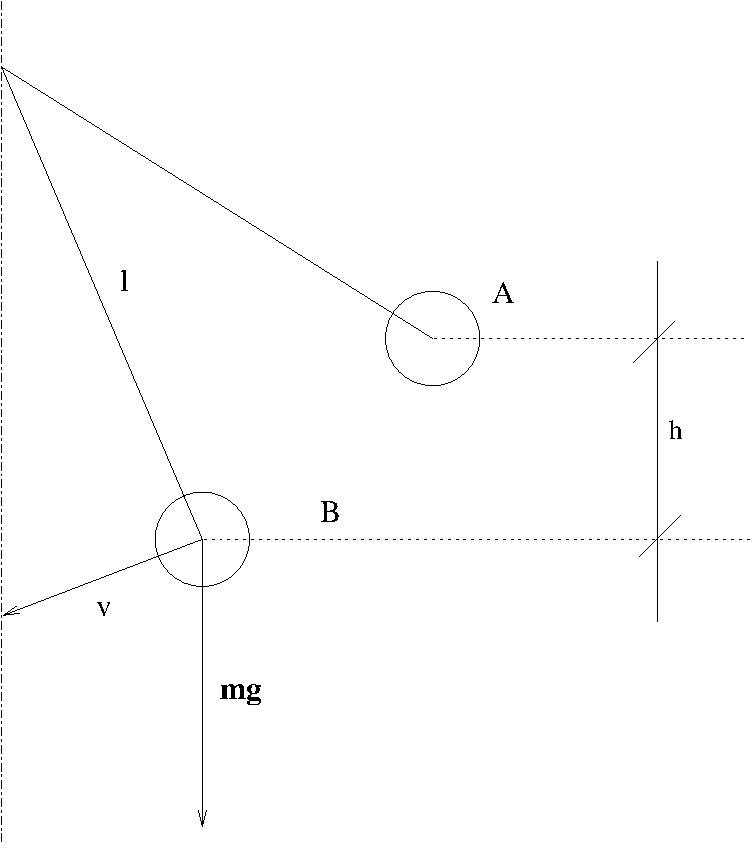
\includegraphics[scale=0.4]{immagini/fisica1/Pendolo_energia}
\end{figure}
Angoli non piccoli, $\ve T\bot \ve v \qquad \ve T\bot \ud\ve s$
\begin{equation*}\delta L=\ve T \cdotp \ud\ve s=0\end{equation*}
\begin{equation*}U=mgh \qquad K=\frac{1}{2}mv^2\end{equation*}
\begin{equation*}mgh+\frac{1}{2}mv^2=E=\const\end{equation*}
A $\theta_0$ si trova nella posizione $A\quad K_A=0$
\begin{equation*}E_A=0+mgh\end{equation*}
In $B$ $K_B\neq 0\quad E_B=K+mgh_B$
\begin{equation*}h=l-l\cos\theta\end{equation*}
\begin{equation*}E_A=mg\left(l-l\cos\theta_0\right)\end{equation*}
\begin{equation*}E_B=\frac{1}{2}mv^2+mg\left(l-l\cos\theta\right)\end{equation*}
\begin{equation*}E_A=E_B\end{equation*}
\begin{equation*}mgl\left(1-\cos\theta_0\right)=\frac{1}{2}mv^2+mgl\left(1-\cos\theta\right)\end{equation*}
\begin{equation*}v^2=2gl(\cos\theta-\cos\theta_0)\end{equation*}

\begin{Es}[arriva in alto?]
\begin{figure}[htbp]
\centering
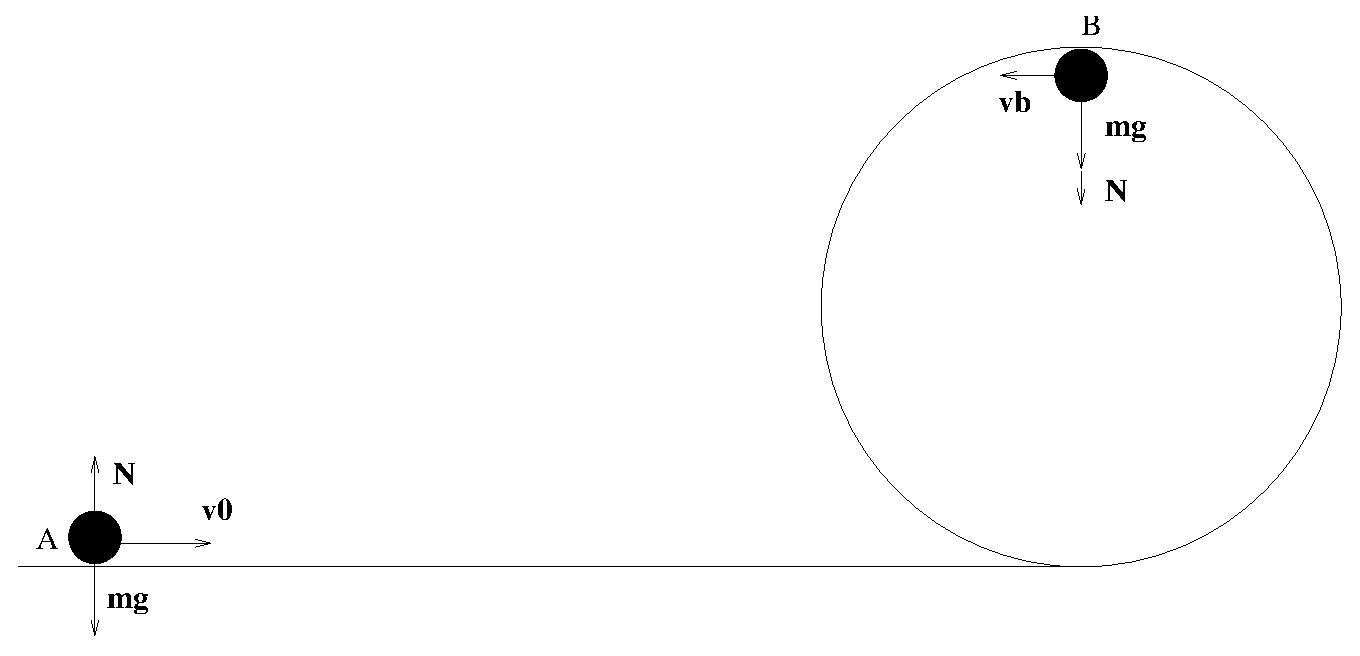
\includegraphics[scale=0.4]{immagini/fisica1/arriva_in_alto}
\end{figure}
La $\ve N$ non compie lavoro perché $\ve N\bot \ud\ve s$
\begin{equation*}E_A=\frac{1}{2}mv_0^2 \qquad E_B=\frac{1}{2}mv_B^2+mg2R\end{equation*}
\begin{equation*}E_A=E_B \quad E_A=\frac{1}{2}mv_0^2=\frac{1}{2}mv_B^2+mg2R\end{equation*}
\begin{equation*}v_0^2=v_B^2+4gR\end{equation*}
Quando è in B
\begin{equation*}mg+N=m\frac{v_B^2}{R}\qquad N=m\frac{v_B^2}{R}-mg\quad \text{per non cadere:}\quad N\geq0\end{equation*}
\begin{equation*}m\frac{v_B^2}{R}\geq mg\qquad v_B^2\geq gR\end{equation*}
\begin{equation*}v_{B\text{min}}^2=gR\qquad v_{0\text{min}}^2=gR+4gR\qquad v_{0\text{min}}=\sqrt{5gR}\end{equation*}
\end{Es}

\chapter{\index{gravitazione}Gravitazione}
\section{Cenni storici}
I sistemi gravitazionali storici più celebri sono stati:
\begin{itemize}
\item[--]\index{sistema!tolemaico}sistema tolemaico. \`E un sistema geocentrico del II
sec.\ d.C.\@ Per ovviare ad alcuni errori, senza uscire dal dogma
delle orbite circolari, Tolomeo suppose che i pianeti
descrivessero degli epicicli
\item[--]\index{sistema!copernicano}sistema copernicano. \`E un sistema eliocentrico del 1500
d.C.
\item[--]\index{sistema!ticonico}sistema ticonico di T.Brahe. \`E un sistema misto tra il sistema
eliocentrico e geocentrico
\end{itemize}

Newton verso il 1665 teorizzò che le leggi celesti sono uguali a quelle terrestri: è una delle prime unificazioni di forze ritenute inizialmente diverse in un'unica forza.

\subsection{\index{leggi!di Keplero}\index{Keplero}Leggi di Keplero}
Le leggi di Keplero sono leggi empiriche, formulate prima delle
teorie di Newton:
\begin{legge}[Prima legge di Keplero]
I pianeti descrivono intorno al Sole orbite ellittiche di cui il Sole occupa uno dei due fuochi. \end{legge}
\begin{legge}[Seconda legge di Keplero]
 Le aree descritte dal raggio vettore tracciato dal Sole ai pianeti sono proporzionali al periodo.
\end{legge}
\begin{legge}[Terza legge di Keplero]
I quadrati dei tempi impiegati dai pianeti a descrivere le proprie orbite sono proporzionali ai cubi dei semiassi maggiori delle ellissi.
\end{legge}


\section{\index{teorema!di Gauss!per la gravità}Teorema di Gauss (per la gravità)}
Con il teorema di Gauss si può supporre che gli effetti della
gravità di un corpo su un altro, al suo esterno, siano uguali a
quelli che si avrebbero se le masse fossero concentrate nel centro
di massa.



\subsection{Caso crosta sferica}
$\ud A$ è l'area compresa tra le due sezioni.
\begin{figure}[htbp]
   \centering
   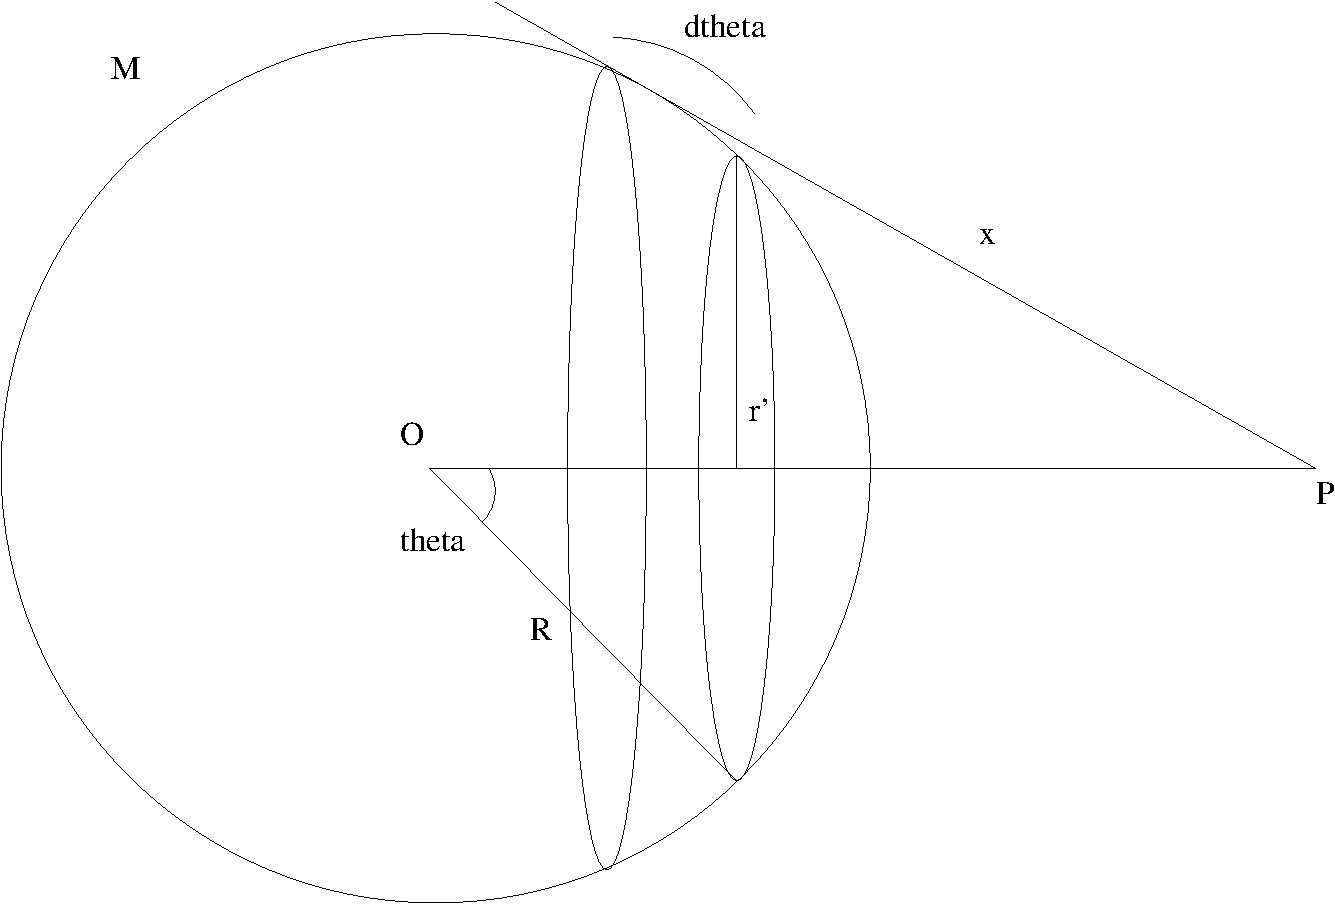
\includegraphics[scale=0.3]{immagini/fisica1/crosta}
\end{figure}
\begin{equation*}F=G\frac{Mm}{r^2}\end{equation*}
\begin{equation*}r'=R\sin\theta\qquad \ud A=2\pi r'R\ud\theta\end{equation*}
$$\frac{\ud m}{M}=\frac{\ud
A}{4\pi R^2}=\frac{2\pi r'R\ud\theta}{4\pi
R^2}=\frac{R\sin\theta\ud\theta}{2R}=\frac{\sin\theta\ud\theta}{2}$$
\begin{equation*}\ud m=\frac{M\sin\theta\ud\theta}{2}\end{equation*}
\begin{equation*}U=-\frac{Gmm'}{r}\qquad\ud U=-\frac{G\ud m m'}{x}\end{equation*}
\begin{equation*}x^2=R^2+r^2-2rR\cos\theta\end{equation*}
Derivando a sinistra in $x$ e a destra in $\theta$ si ha:
\begin{equation*}2x\,\ud x=2rR\sin\theta\ud\theta\sin\theta\ud\theta\end{equation*}
\begin{equation*}\sin\theta\ud\theta=\frac{x\ud x}{rR}\end{equation*}
\begin{align*}
U&=-\int_{\text{palla}}\frac{Gm'}{x}\,\ud
m=-\int_{\text{palla}}\frac{Gm'}{x}\frac{M\sin\theta\ud\theta}{2}=-\frac{Gm'
m}{2}\int_{\text{palla}}\frac{\sin\theta}{x}\ud\theta\\
&=-\frac{Gmm'}{2rR}\int\frac{x}{x}\ud
x=-\frac{Gmm'}{2rR}\int_{r-R}^{r+R}\ud
x=-\frac{Gmm'}{2rR}[r+R-r+r]\\
&=-\frac{Gmm'}{2rR}2R=-\frac{Gmm'}{r}
\end{align*}
Possiamo quindi concentrare tutta la massa nel centro della palla (se $P$ sta fuori).
Se $P$ è esterno: $$U=-\frac{Gmm'}{r}\qquad F=-\frac{\ud U}{\ud
r}=\frac{Gmm'}{r^2}$$
Se $P$ è interno vale il discorso precedente fino alla scelta degli
estremi:
\begin{align*}
U(P)&=-\frac{Gmm'}{2rR}\int_{R-r}^{r+R}\ud x=-\frac{Gmm'}{2rR}[r+R-R+r]\\
&=-\frac{Gmm'}{2rR}2r=-\frac{Gmm^2}{R}=\const
\end{align*}
\begin{equation*}\ve F=-\frac{\ud U}{\ud \ve r}=0\end{equation*}

Quindi un punto all'interno del guscio non risente di alcuna
forza, questo lo si può dimostrare ragionando con in coni, in
quanto per ogni cono le forze sono uguali.

\begin{figure}[htbp]
\centering
\subfigure[Ideale]{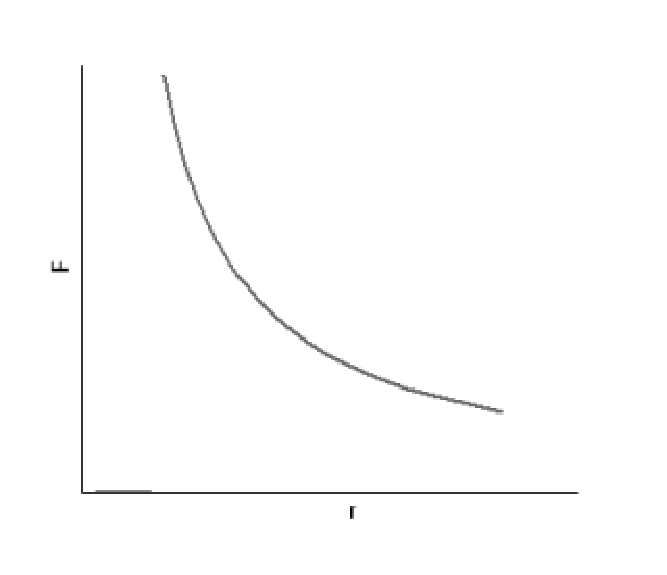
\includegraphics[scale=0.6]{immagini/fisica1/gr_ideal_cava}}\quad
\subfigure[Reale]{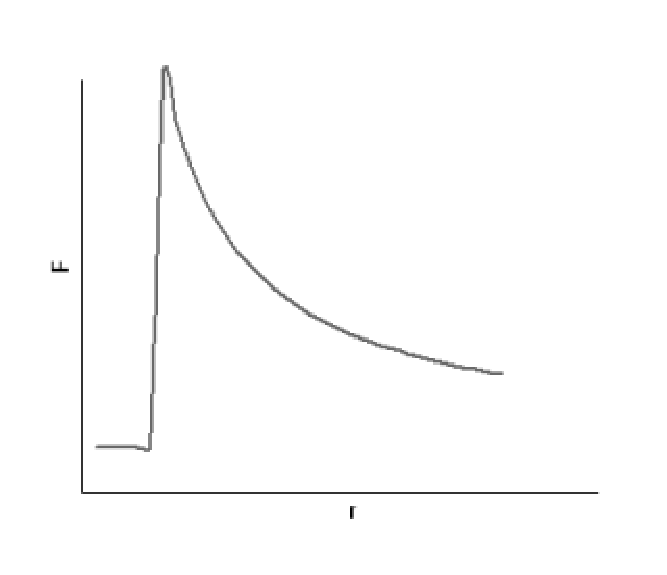
\includegraphics[scale=0.6]{immagini/fisica1/gr_real_cava}}
\caption{Forza in una sfera cava ideale (a) e reale (b)}
\end{figure}

\subsection{Caso sfera piena}

All'esterno:
\begin{equation*}F=-G\frac{Mm'}{r^2}\end{equation*}
Dentro:
\begin{equation*}F=-G\frac{M^{\text{int}}m'}{r^2}\end{equation*}
\begin{equation*}\frac{M^{\text{int}}}{M^{\text{tot}}}=\frac{V^{\text{int}}}{V^{\text{tot}}}=\frac{\frac{4}{3}\pi r^2\rho}{\frac{4}{3}\pi R^3\rho}\end{equation*}
\begin{equation*}M^{\text{int}}=\frac{r^3}{R^3}M^{\text{tot}}\end{equation*}
\begin{equation*}F=-\frac{Gr^3M^{\text{tot}}m'}{r^2R^3}=-\frac{Gmm'r}{R^3}=-kr\end{equation*}
ha l'espressione di una forza elastica.

\begin{Es}[posta pneumatica interterrestre]
Immaginiamo di fare un buco che attraversa tutta la terra, passando per il centro. Un pacco lanciato al suo interno sarebbe sottoposto ad una forza del tipo:
\begin{equation*}F=-kr\qquad k=\left(G\frac{m'M_T}{R_T^3}\right)\end{equation*}
\begin{equation*}T=2\pi\sqrt{\frac{m'}{k}}=2\pi\sqrt{\frac{R_T^3}{GM_T}}=2\pi\sqrt{\frac{R_T}{g}}\simeq \unita{40}\minute\end{equation*}
\end{Es}
\section{Interpretazione delle leggi di Keplero}
\subsection{Seconda legge}

L'unica ipotesi che utilizziamo è che la forza sia centrale,
quindi il risultato è estendibile a tutte le forze centrali. Una
forza si dice centrale quando è diretta come la congiungente dei
due punti che interagiscono.

\begin{figure}[htbp]
   \centering
   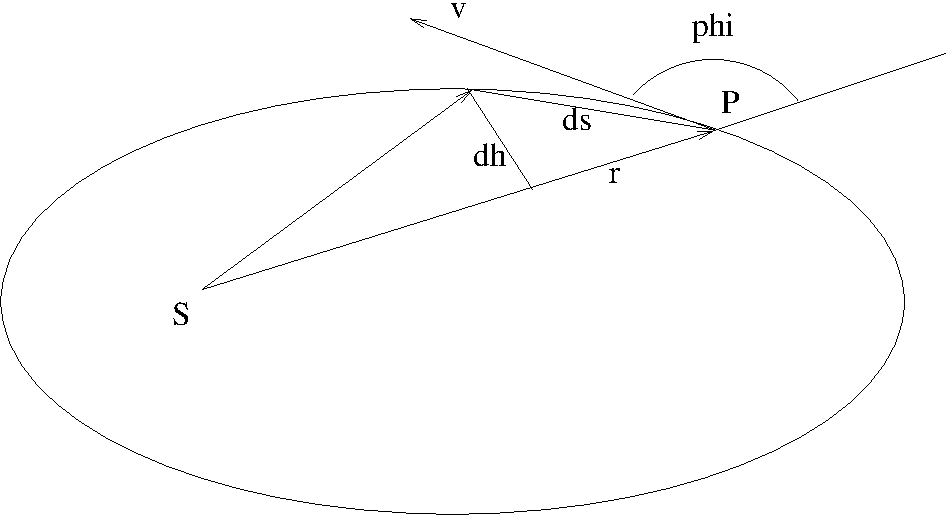
\includegraphics[scale=0.45]{immagini/fisica1/keplero}
\end{figure}



$$\frac{\ud\ve L_S}{\ud t}=\ve\tau_S=0\quad\text{perché }\ve
F\parallel\ve r$$
\begin{equation*}\ve L_S=\ve r\times m\ve v=\overrightarrow{\const}\end{equation*}
\begin{equation*}L_S=rmv\sin\phi={\const}\end{equation*}
\begin{equation*}\ud h=\ud s\sin\phi\end{equation*}
$$\text{velocità areolare}=\frac{\ud A}{\ud t}=\frac{r\ud h}{2\ud
t}=\frac{r\sin\phi\ud s}{2\ud t}=\frac{r}{2}v\sin\phi$$
$$L_S=\frac{\ud A}{\ud t}2m\qquad\frac{\ud A}{\ud
t}=\frac{L_S}{2m}=\const$$
\subsection{Terza legge}
\begin{equation*}F=\frac{GM_Sm}{R^2}=ma=\frac{mv^2}{R}=\omega^2Rm\end{equation*}
\begin{equation*}\frac{GM_S}{R^2}=\omega^2R\qquad \omega=\frac{2\pi}{T}\end{equation*}
$$\frac{GM_S}{R^2}=\frac{4\pi^2}{T^2}R\qquad
T^2=\frac{4\pi^2}{GM_S}R^3$$
\begin{equation*}\frac{T^2}{R^3}=\frac{4\pi^2}{GM_S}=\const\end{equation*}

\section{\index{accelerazione!di gravità}Accelerazione di gravità}
\begin{equation*}\ve g=\frac{\ve F}{m}\end{equation*}
Sulla Terra: \begin{equation*}g = \frac{G\frac{M_Tm}{R_T^2}}{m}=\frac{GM_T}{R_T^2}\simeq \unita{9.836}\meter\per\second\squared\end{equation*}
In realtà questo valore è variabile, dall'equatore ai poli, cioè
circa tra $9.78\div9.86$, a causa della forza centrifuga e dallo
schiacciamento dei poli. Per quanto riguarda la forza centrifuga
questa è nulla ai poli e massima all'equatore quindi:
\begin{equation*}F_C=m\omega^2R\qquad F_N=mg_{\text{polo}}\end{equation*}
\begin{equation*}\frac{F_C}{F_N}=\frac{\omega^2R}{g_{\text{polo}}}=\frac{(2\pi)^2}{T^2}\frac{R}{g_{\text{polo}}}\end{equation*}
\section{\index{bilancia!di torsione}Misurazione della costante di gra\-vi\-ta\-zio\-ne u\-ni\-ver\-sa\-le}
Cavendish con l'articolo ``Misura della massa terrestre'' nel
1798 è il primo a misurare la costante di gravitazione universale
o costante di Cavendish. Cavendish si proponeva di misurare la
massa terrestre e quindi indirettamente $G$.

La bilancia di torsione viene fatta oscillare, il momento è
proporzionale all'angolo di scostamento dalla posizione di
equilibrio, si genera un moto armonico.

\begin{equation*}\tau=-k\theta=I\alpha\qquad\alpha=\frac{\ud^2\theta}{\ud t^2}\end{equation*}
\begin{equation*}-k\theta=I\ddot\theta\qquad T=2\pi\sqrt\frac{I}{k}\qquad I=2mD^2\end{equation*}


Da qui sperimentalmente si trova $k$. Avvicinando delle masse più
grosse si genera un momento dovuto alla forza gravitazionale. Si
impone che il momento gravitazionale sia uguale al momento dovuto
alla forza elastica di richiamo.

\begin{equation*}\tau_\text{Newton}=2\frac{GMm}{d^2}D=\tau_\text{torsione}=k\theta\end{equation*}
\begin{equation*}G=\frac{k\theta d^2}{2MmD}\end{equation*}
\section{Massa gravitazione e massa inerziale}
Per massa inerziale si intende quella grandezza usata in dinamica
per esempio \mbox{$\ve F=m\ve a$}. Per massa gravitazionale si intende quella usata nella gravitazione per esempio $F=G\frac{Mm}{r^2}$. Anche se la questione è aperta $m_i$ è proporzionale a $m_g$ infatti se $B$ e $C$ sono attratti da $A$ si ha:
\begin{equation*}\frac{F_{BA}}{F_{CA}}=\frac{Gm_{Bg}m_{ag}}{Gm_{Cg}m_{ag}}=\frac{m_{Bg}}{m_{Cg}}=\frac{m_{Bi}a_b}{m_{ci}a_c}\end{equation*}
$$\text{se }a_C=a_B\Rightarrow\frac{m_{Bg}}{m_{Cg}}=\frac{m_{Bi}}{m_{Ci}}\Rightarrow
m_{Bg}=\frac{m_{Cg}}{m_{Ci}}\cdot m_{Bi}$$
\section{\index{principio!di equivalenza}Principio di equivalenza}
\begin{Pri}[equivalenza di Einstein]
nessun esperimento può rivelare la differenza tra un sistema di riferimento inerziale immerso in un campo gravitazionale $\ve j$ e un sistema non inerziale con accelerazione costante $\ve a=-\ve j$
\end{Pri}
\section{\index{energia!di un'orbita}Energia associata ad un'orbita}
\begin{equation*}E=\frac{1}{2}mv^2-G\frac{Mm}{r^2}=-G\frac{Mm}{2a}\end{equation*}
\begin{equation*}r(\theta)=\frac{p}{1+e\cos\theta}\end{equation*}
\begin{equation*}p=\frac{L^2}{m\alpha}\end{equation*}
\begin{equation*}\alpha=GMm\end{equation*}
\begin{equation*}e=\text{eccentricità}=\sqrt{1+2^{\frac{EL^2}{m\alpha}}}\end{equation*}
$$\begin{array}{llc}
e>1&E>0&\text{iperbole}\\
e=1&E=0&\text{parabola}\\
0<e<1&E<0&\text{ellisse}\\
e=0&E<0&\text{circonferenza}\\
\end{array}$$

\chapter{\index{meccanica dei fluidi|(}Meccanica dei fluidi}
\minitoc
Un fluido è un liquido o un gas. La meccanica dei fluidi applica le leggi della meccanica classica ai fluidi descrivendo tutto in termini di pressione, volume, portata.
\section{\index{fluidostatica}Fluidostatica}
\subsection{\index{pressione}Pressione e \index{densità}densità}
La pressione è la forza sull'unità di superficie: $p=\frac{\ud |\ve F|}{\ud A}$. \`E una grandezza scalare, infatti la forza agisce sempre perpendicolarmente alla superficie. Se avesse una componente tangenziale il fluido si muoverebbe e non parleremmo più di fluidostatica. Un altro modo analogo usando il vettore normale è
\begin{Def}[pressione]
\begin{equation}
p=\frac{\ud\ve F\cdot \ve n}{\ud A}
\end{equation}
\end{Def}
La pressione si misura in: $\newton\per\meter\squared=\pascal$ (pascal), che però è usualmente piccola, comuni sono anche: $\si{}{\bbar}=\si{1E5}{\pascal}$, $\si{}{\atmosphere}=\si{1.013E5}{\pascal}$, $\si{}{\torr}=\si{}{\mmHg}=\si{1/760}{\atmosphere}$.
\begin{Def}[densità locale]
\begin{equation}
\rho(\ve r)=\frac{\ud m}{\ud V}
\end{equation}
\end{Def}
si misura in $\si{}{\kilogram/\metre^3}$.

\subsection{\index{legge!di Stevino}Legge di Stevino}
\label{stevino11}
\begin{figure}[htbp]
\centering
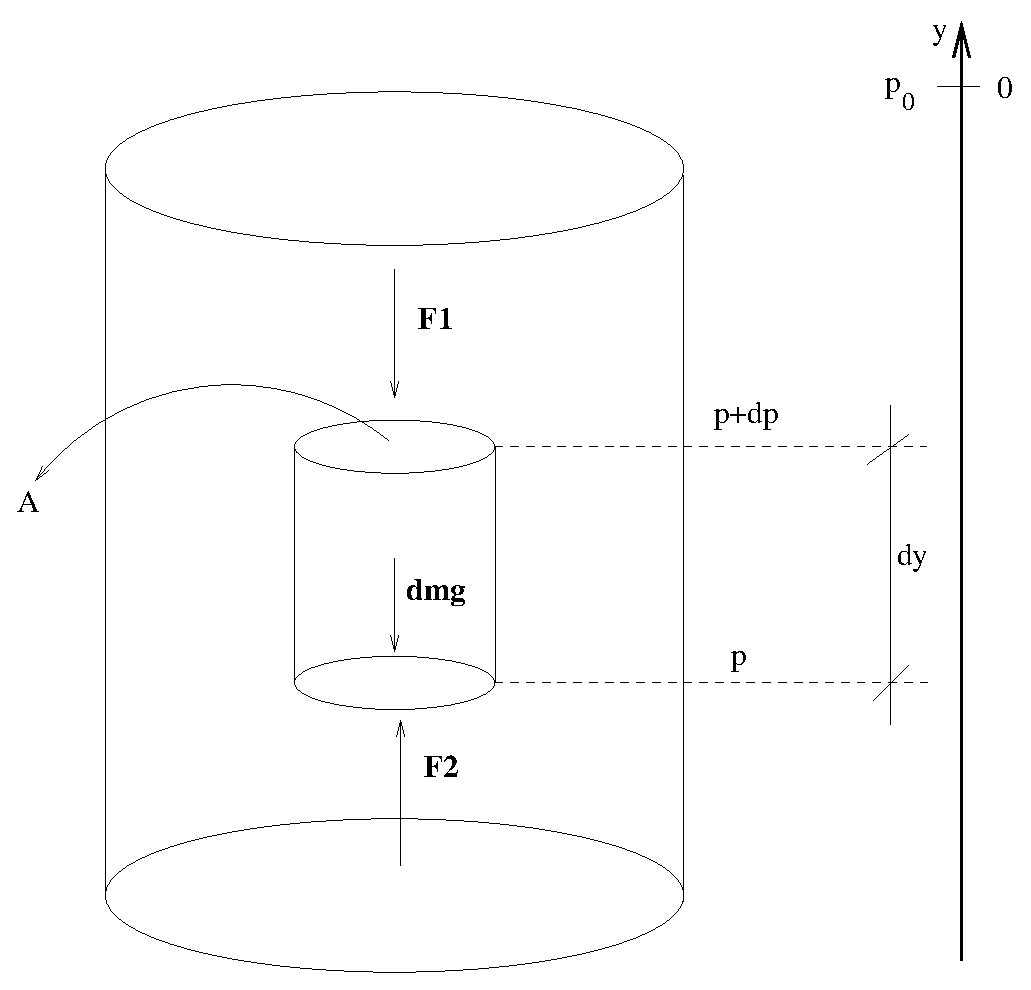
\includegraphics[scale=0.4]{immagini/fisica1/legge_di_stevino1}
\end{figure}


Il fluido è in equilibrio quindi $\ve F_1+\ve F_2+\ud m\ve g=0$. $\ve F_1$ è la forza dovuta alla pressione della parte superiore del fluido, $\ve F_2$ a quella inferiore.
\[-\ud mg-(p+\ud p)A+pA=0\qquad -\ud mg-dpA=0\]
\[\ud m=\rho \ud V=\rho A\ud y\qquad -\rho A\ud y g-\ud p A=0\]
\[\ud p=-\rho g \ud y\]
\[p_0=\text{pressione atmosferica}\]
\[\text{Integrando: }\int_{p_0}^p \ud p=-\int_0^y \rho g\,\ud y=-\rho g\int_0^h\!\ud y\]
\[p=p_0-\rho g y = p_0+\rho g h\]
che è la legge di Stevino e $h$ è la profondita, valida se consideriamo la densità costante, come per esempio in un liquido, per un gas ciò non è più possibile quindi ipotizzando che \[\frac{\rho}{\rho_0}=\frac{p}{p_0}\quad\Rightarrow\quad \rho=\rho_0\frac{p}{p_0}\]
\[\ud p=-\rho_0\frac{p}{p_0}g\ud y\qquad \int_{p_0}^p \frac{\ud p}{p}=\int_0^y -\rho_0\frac{g}{p_0}\ud y\]
\[\log p-\log p_0=\log\frac{p}{p_0}=-\rho_0\frac{g}{p_0}y\]
\begin{equation}
p=p_0e^{-\frac{\rho_0 g}{p_0}y}
\label{legge_atmosfera}
\end{equation}
\[p=p_0e^{-\frac{y}{\lambda}}\qquad \lambda=\frac{p_0}{\rho_0 g}\quad \text{è una lunghezza}\]
che è la legge dell'atmosfera.

\subsection{\index{legge!dei vasi comunicanti}Legge dei vasi comunicanti}
Nel tubo a U (fig.\@\ref{vasicom}) sono introdotti due liquidi non miscibili 1 e 2. Sotto ad A e B c'è solo il fluido 2. A e B sono alla stessa altezza, quindi per la legge di Stevino devono avere la stessa pressione infatti il punto inferiore del tubo ad U avrà una certa pressione $P_{\max}$, la pressione nel punto $A$ sarà $P_{\max} - \rho_a g h_{OA}$ e nel punto $B$ $P_{\max} - \rho_a g h_{OB}$, ma $h_{OA}=h_{OB}$. Usando ancora la legge di Stevino:
\begin{figure}[htbp]
\centering
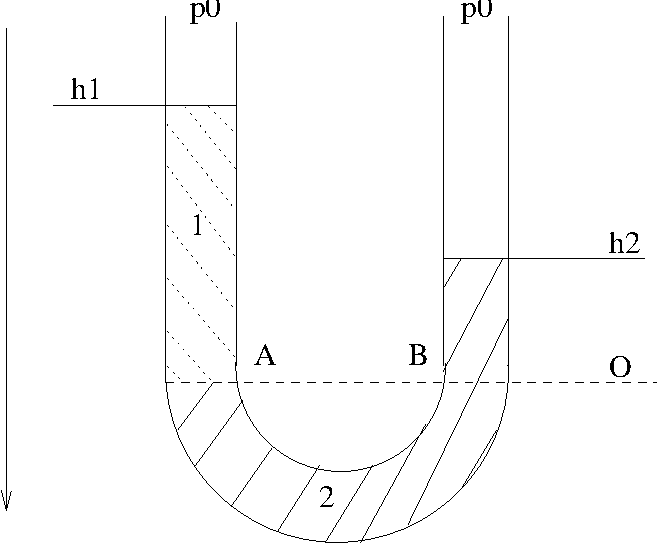
\includegraphics[scale=0.5]{immagini/fisica1/vasi_comunicanti}
\caption{Vasi comunicanti.}
\label{vasicom}
\end{figure}
\[p_A=p_B\qquad p_0+\rho_1 gh_1=p_0+\rho_2gh_2\]
\[\text{legge dei vasi comunicanti: }\frac{\rho_1}{\rho_2}=\frac{h_2}{h_1}\]
in particolare se $\rho_1=\rho_2$ allora $h_1=h_2$.
\subsection{Esperimento di \index{Torricelli}\index{esperimento!di Torricelli}Torricelli}
L'esperimento del 1664 (fig.\@\ref{estor}) consiste nel riempire fino all'orlo un cilindro di mercurio e di rovesciarlo, senza far uscire il liquido, in una bacinella in cui c'è già del mercurio. Il livello del mercurio scende nel cilindro fino al livello di \si{0.76}{\meter}.
\begin{figure}[htbp]
\centering
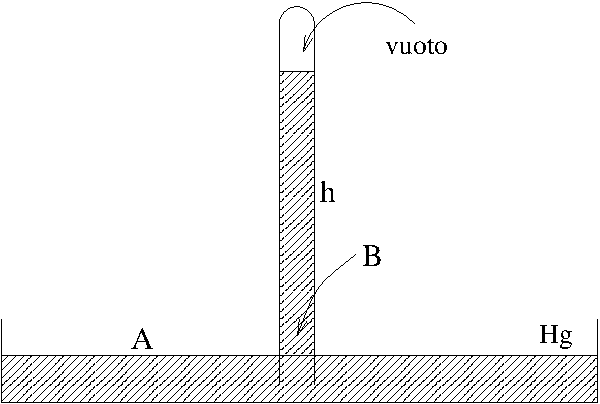
\includegraphics[scale=0.7]{immagini/fisica1/Torricelli}
\caption{Esperimento di Torricelli.}
\label{estor}
\end{figure}

Il punto A e il punto B sono allo stesso livello, quindi: $p_A=p_B$
\[p_A=p_0\qquad p_B=\rho_{\mathrm{Hg}}gh\qquad p_0=\rho_\mathrm{Hg}gh=\si{1}{\atmosphere} \]
Si misura in questo modo la pressione atmosferica, in $\mmHg$.\index{pressione! atmosferica}

L'esperimento di Torricelli suscitò clamore perché Torricelli suppose che nella zona superiore del tubo ci ``fosse'' del vuoto.\index{vuoto}

\subsection{Esperimento delle due semisfere\index{esperimento!delle due semisfere}}
In due semisfere attaccate in modo da creare una sfera unica viene diminuita la pressione togliendo aria. In questo modo la pressione esterna è maggiore ed esercita una forza sulle pareti delle semisfere, rendendo difficile la separazione.
\begin{figure}[htbp]
\centering
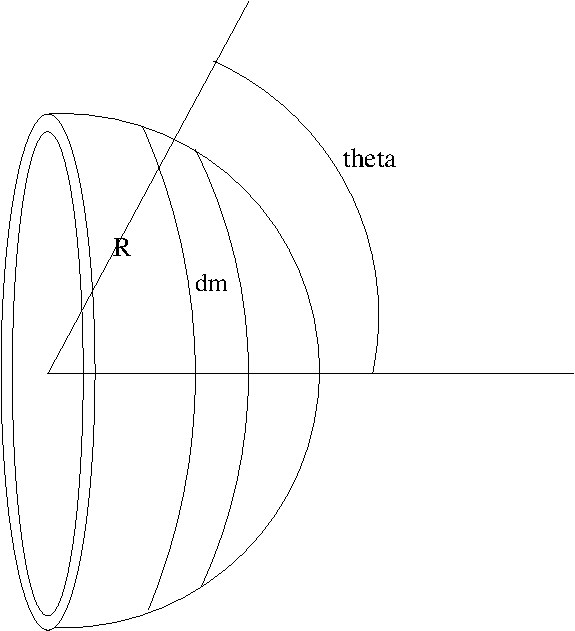
\includegraphics[scale=0.5]{immagini/fisica1/Sfera_pressione}
\end{figure}

Consideriamo la strisciolina $\ud m$
\[F=\int\ud F\]
\[\ud A=2\pi R\sin\theta R\ud\theta=2\pi R^2\sin\theta\ud\theta\]
\[\ud F_x=p_0 \ud A\cos\theta\]
\[\frac{\ud \sin\theta}{\ud \theta}=\cos\theta\qquad\ud\sin\theta=\cos\theta\ud\theta\]
\[\int_S \ud F_x=p_0 2\pi R^2\int_0^{\frac{\pi}{2}}\sin\theta\cos\theta\ud\theta=p_0 2\pi R^2\int_0^{1}\sin\theta\ud(\sin\theta)=p_0\pi R^2\]
\[\text{se } R=\SI{1}{\metre} \quad F_x\simeq\SI{3E5}{\newton} \]

\subsection{Principio di Pascal\index{principio!di Pascal}}
\begin{Pri}[Pascal]
 La variazione di pressione dovuta a forze esterne si trasmette invariata in tutti i punti del fluido.
\end{Pri}

Consideriamo un cilindro con un pistone che non esercita pressione.

\begin{figure}[htbp]
\centering
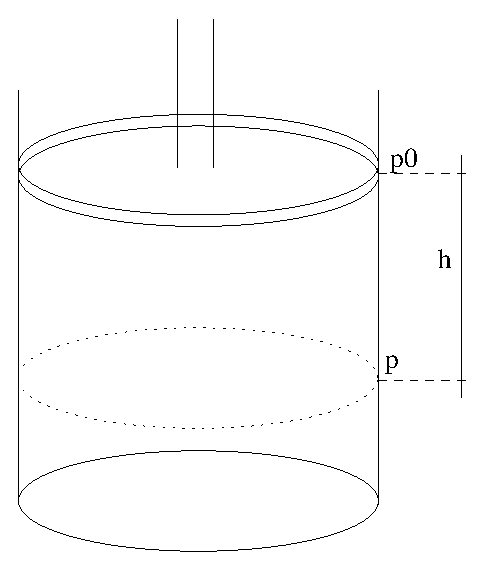
\includegraphics[scale=0.5]{immagini/fisica1/Pascal1}
\end{figure}

Se applichiamo una forza sul pistone la pressione esterna, al livello del pistone, salirà da $p_0$ a $p_0+p_0'$
\begin{align*}
\text{Prima:}&\quad p=p_0+\rho gh\\
\text{Dopo:}&\quad p=p_0+p_0'+\rho gh=p+p_0'
\end{align*}
cioè la variazione di pressione si trasmette in tutti i punti del fluido.
\subsubsection{Paradosso di Pascal}
Pascal si divertiva a rompere le botti infilandogli un tubo molto lungo, anche di sezione sottile, in quanto la sezione non conta, pieno d'acqua. La pressione faceva rompere le botti.

\subsection{Principio di Archimede\index{principio!di Archimede}}
Consideriamo un elemento di un fluido. Su di esso agisce la forza peso, perché sia in equilibrio deve agire una forza uguale e contraria: la spinta di Archimede $\ve S=-\rho V\ve g$. Essa è dovuta alla differenza di pressione $\Delta p$. Se sostituiamo l'elemento di fluido con un solido il contorno non cambia e quindi la spinta di Archimede risulta uguale. Il peso però è cambiato, quindi in generale non è in equilibrio, infatti la somma delle forze:
\[
 \rho V\ve g - \rho_\text{fluido}V\ve g \neq 0
\]
Se $P>S$ cioè $\rho>\rho_\text{fluido}$ sprofonda, altrimenti il corpo sale e bisogna considerare che una parte di questo emergerà e allora la spinta di Archimede diminuirà. La condizione di equilibri in questo caso è:
\[
 \rho V\ve g - \rho_\text{fludio}V_\text{immerso}\ve g = 0
\]
la soluzione è $V_\text{immerso}=\frac{\rho}{\rho_\text{fluido}}V$ e poiché è sicuramente vero che $V_\text{immerso}\leq V$ allora deve essere $\rho\leq\rho_\text{fluido}$.


\begin{Es}[Iceberg]
\marginpar{
\begin{tiny}ecco quello che dicono i nostri matematici\end{tiny}

\includegraphics[scale=1.4]{immagini/fisica1/firma_daniele}
}
Ghiaccio in acqua $\Longrightarrow$ si scioglie
\[V_\text{totale}-V_\text{emergente}=V_\text{totale}\frac{\rho_\text{ghiaccio}}{\rho_\text{\ce{H2O}}}\]
\[V_\text{totale}\simeq 10 V_\text{emergente}\]
\end{Es}
\subsection{Condizione generale di equilibrio}
\begin{figure}[htbp]
   \centering
   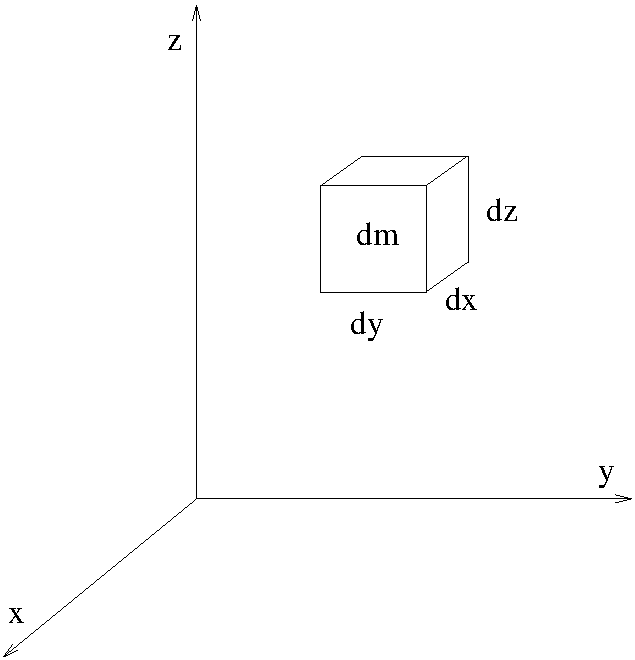
\includegraphics[scale=0.4]{immagini/fisica1/equilibrio}
\end{figure}
Forze di volume: proporzionali al volume
\[\ve f=\frac{\ve F}{m}\]
notare che $\ve f$ è un'accelerazione.


Forze di superficie: dovute al liquido che lo circonda, proporzionali alla superficie
\[F=pA\]
Lungo l'asse $x$:

\[f_x\ud m+p(x)\ud z\ud y-p(x+\ud x)\ud y\ud z=0\]
\[f_x\rho\ud x\ud y\ud z+p(x)\ud y\ud z-(p(x)+\frac{\partial p}{\partial x}\ud x)\ud y\ud z=0\]
\[f_x\rho\ud x\ud y\ud z-\frac{\partial p}{\partial {x}}\ud x\ud y\ud z=0\]
\[f_x\rho=\frac{\partial p}{\partial x}\quad f_y\rho=\frac{\partial p}{\partial y}\quad f_z\rho=\frac{\partial p}{\partial z}\]
\begin{equation}\ve f\rho=\ve\nabla p\end{equation}

\begin{Es}[Forza peso -- Stevino]
Nelle ipotesi di Stevino c'è solo il peso, quindi $\ve f=\ve g$
\[
f_z\rho=\frac{\ud p_z}{\ud z}\quad g\rho\ud z=\ud p \quad p=p_0+\rho gz
\]
In generale:
\[U_m=\frac{U}{m}\qquad \rho\ve f=-\rho\ve\nabla(U_m)=\ve\nabla p\qquad -\ve\nabla(\rho U_m)=\ve\nabla p\]
\[\rho U_m=-p+\const\]
Segue che le superficie isobariche \index{superficie!isobarica}coincidono con le superfici equipotenziali. Nel caso agisca solo la forza peso esse sono dei piani orizzontali: $U_m = -gz+U_0$.
\end{Es}
\begin{Es}[Fluido in accelerazione]
 \begin{figure}[htbp]
 \centering
 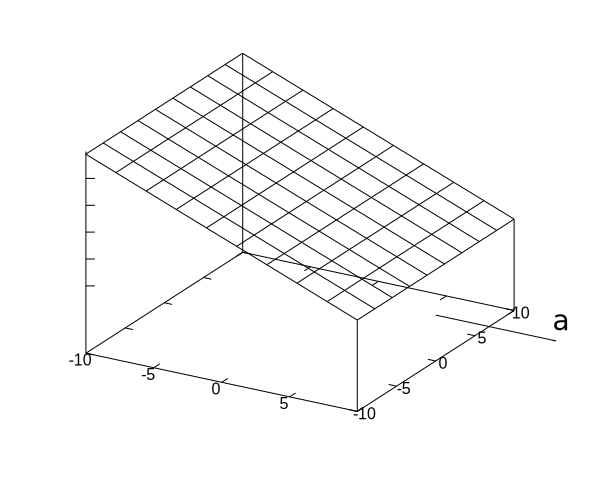
\includegraphics[scale=0.5]{immagini/fisica1/fluido_accelerato}
 % fluido_accelerato.pdf: 480x384 pixel, 72dpi, 16.93x13.55 cm, bb=0 0 480 384
\end{figure}
 Se un fluido è accelerato verso destra con accelerazione $a$ allora usando le forze fittizie: $\ve F=m\ve g-m\ve a$:
\[
 \ve f = -g\ver j - a \ver i
\]
l'equazione differenziale risultante:
\[
 \begin{cases}
  -a\rho=\frac{\partial p}{\partial x}\\
  -g\rho=\frac{\partial p}{\partial y}
 \end{cases}
\]
la cui soluzione è:
\[
 p = \rho(-ax-gy)
\]
e le superfici isobariche (ed equipotenziali):
\[
 y = -\frac{p}{\rho g} - \frac{a}{g}x
\]
che è un piano la cui pendenza è proporzionale all'accelerazione del sistema.
\end{Es}
\begin{Es}[Fluido in rotazione\index{moto!circolare!di un fluido}]
\begin{figure}[htbp]
\centering
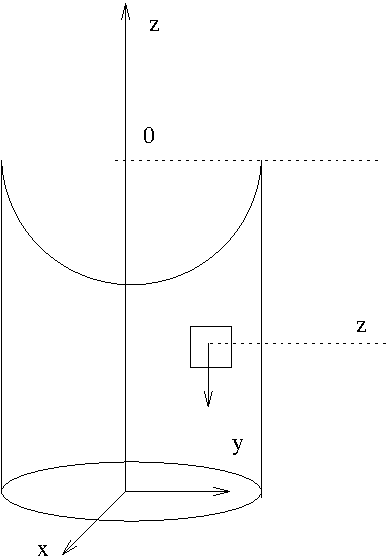
\includegraphics[scale=0.65]{immagini/fisica1/fluido_rotazione}
\caption{Elemento di un fluido in rotazione.}
\end{figure}
Per lavorare in un sistema non inerziale ed usare la legge di Newton aggiungiamo la forza fittizia $m\omega^2 r$, $r$ è la distanza dal centro, la distanza dell'elemento $\ud m$ dall'asse.
\[\text{Nella direzione radiale } f_r=\omega^2 r\]
\[f_r\rho=\rho\omega^2 y=\frac{\ud p}{\ud y}\qquad \ud p=\rho\omega^2 y\ud y\]
\[\int_{p_\text{asse}}^p\ud p=\int_0^R \rho\omega^2 y\ud y\]
\[p-p_\text{asse}=\rho\omega^2\frac{R^2}{2}\qquad p=p_\text{asse}+\frac{\rho\omega^2}{2}R^2\]
\[p_\text{asse}=p_0-\rho gz\qquad p=p_0-\rho gz+\frac{\rho\omega^2}{2}R^2\]
Su una superficie isobarica $p=\const$,
\[\rho gz=\const+\frac{\rho\omega^2}{2}R^2\]
\[z=\const+\frac{\rho\omega^2}{2\rho g}R^2=\const+\frac{\omega^2}{2g}R^2=\const+\frac{\omega^2}{2g}(x^2+y^2)\]
\`E un paraboloide:
\begin{figure}[htbp]
\centering
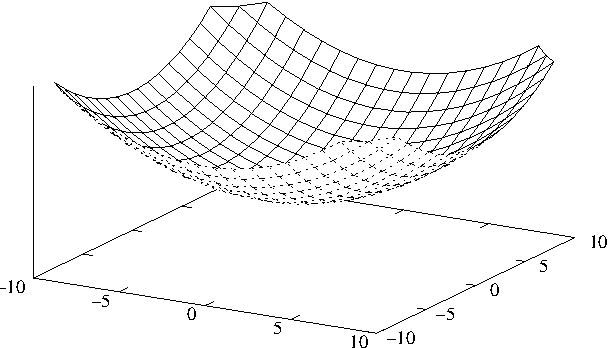
\includegraphics[scale=1]{immagini/fisica1/paraboloide}
\caption{Paraboloide.}
\end{figure}
\subsubsection{Archimede per le rotazioni}
Come per il caso in cui c'è solo la forza di gravità anche nel caso di fluido in rotazione vale lo stesso risultato, cioè che se l'oggetto è meno denso del fluido si sposta verso l'esterno se più denso verso l'interno. Infatti consideriamo solo la forza centrifuga (oppure il limite per $\omega$ molto alto) allora la spinta di archimede verso l'interno sarà: $\rho_\text{fluido}V\omega^2 r$. Allora la somma delle forze verso l'esterno sarà:
\[
 \rho V\omega^2 r-\rho_\text{fluido}V\omega^2 r
\]
quindi a meno che $r=0$ il corpo si muove verso l'esterno se $\rho>\rho_\text{fluido}$. Questo è il principio delle centrifughe.
\end{Es}

\section{Dinamica dei fluidi\index{dinamica!dei fluidi}}
\begin{description}
\item[Approccio di Lagrange\index{Lagrange}]: si danno le coordinate $x$ di un elemento di flusso in funzione del tempo, è un metodo di analisi complicato.
\item[Approccio di Eulero\index{Eulero}]: si studiano le caratteristiche del fluido in un determinato punto. Ci mettiamo in un punto dello spazio e vediamo come variano le grandezze in funzione del tempo. Per descrivere in modo completo bisogna ripetere le misurazioni in modo completo.
\end{description}
Vengono usate le semplificazioni:
\begin{itemize}
\item fluidi:
\begin{itemize}
\item incomprimibili ($\rho=\const$)
\item non viscosi (primi di attrito interno)
\end{itemize}
\item moto:
\begin{itemize}
\item stazionario (i fenomeni non dipendono dal tempo)
\item irrotazionale (nessun vortice, non caotici), $\mathrm{rot}(\ve v)=0$, $\oint \ve v \ud \ve s=0$
\end{itemize}
\end{itemize}
\begin{description}
 \item [Linee di flusso\index{linee!di flusso}]: linee tangenti alla $\ve v$ della particella. Ha senso se il moto è stazionario, cioè se $\ve v$ è costante nel tempo. 
 \item[Tubo di flusso] Le linee di flusso danno origine al tubo di flusso\index{tubo!di flusso}. Non è possibile che vi sia fuoriuscita di fluido latente per definizione: $\ve v$ è tangente alle linee di flusso.
\end{description}

\subsection{Equazione di continuità\index{equazione!di continuità}}
La portata volumica è la quantità di volume che passa nel tempo: $Q=\frac{\ud V}{\ud t}$, ma essendo in regime stazionario la velocità non varia, quindi $Q=\frac{\Delta V}{\Delta t}$, la portata di massa è la quantità di massa nel tempo.

\begin{figure}[htbp]
\centering
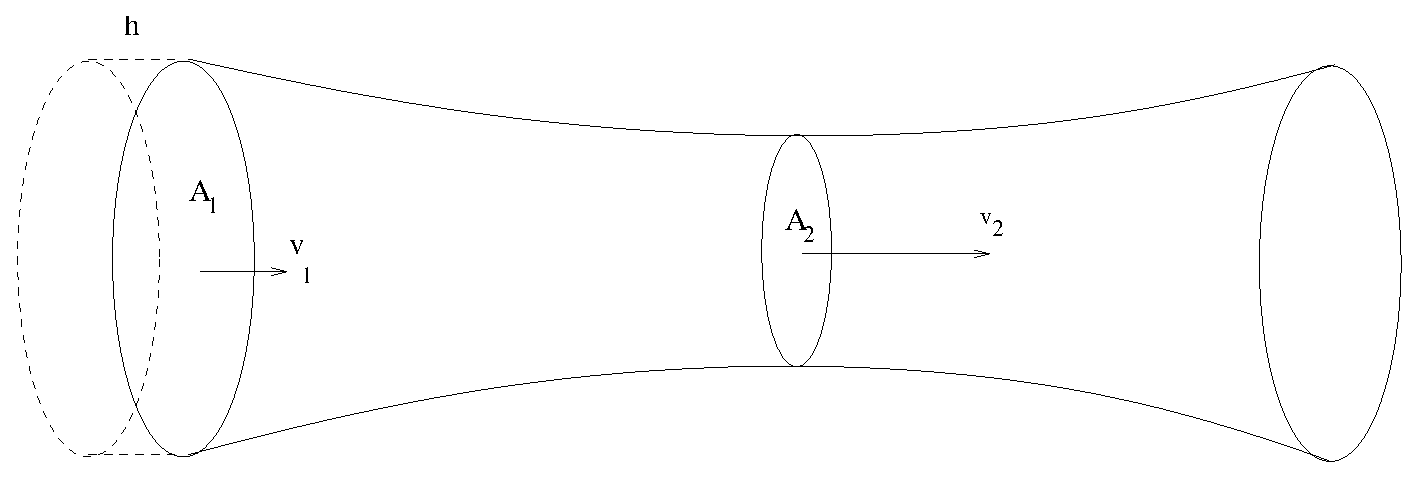
\includegraphics[scale=0.4]{immagini/fisica1/equazione_continuita}
\end{figure}
Fissiamo $\Delta t$ tale che $h=v_1\Delta t$
\begin{enumerate}
\item fluido che entra in $\Delta t\quad \rho\Delta V=\rho A_1v_1\Delta t$
\item fluido che esce in $\Delta t\quad \rho\Delta V=\rho A_2v_2\Delta t$
\end{enumerate}
Naturalmente le masse entranti e uscenti sono uguali, quindi (legge di Leonardo\index{legge!di Leonardo}\index{Leonardo}):
\[A_1v_1=A_2v_2\]

Portata volumica\index{portata!volumica}: $Q_v=Av$

Portata di massa\index{portata!di massa}: $Q_m=\rho Av$

\subsection{Equazione di Bernoulli\index{equazione!di Bernoulli}}


\begin{center}
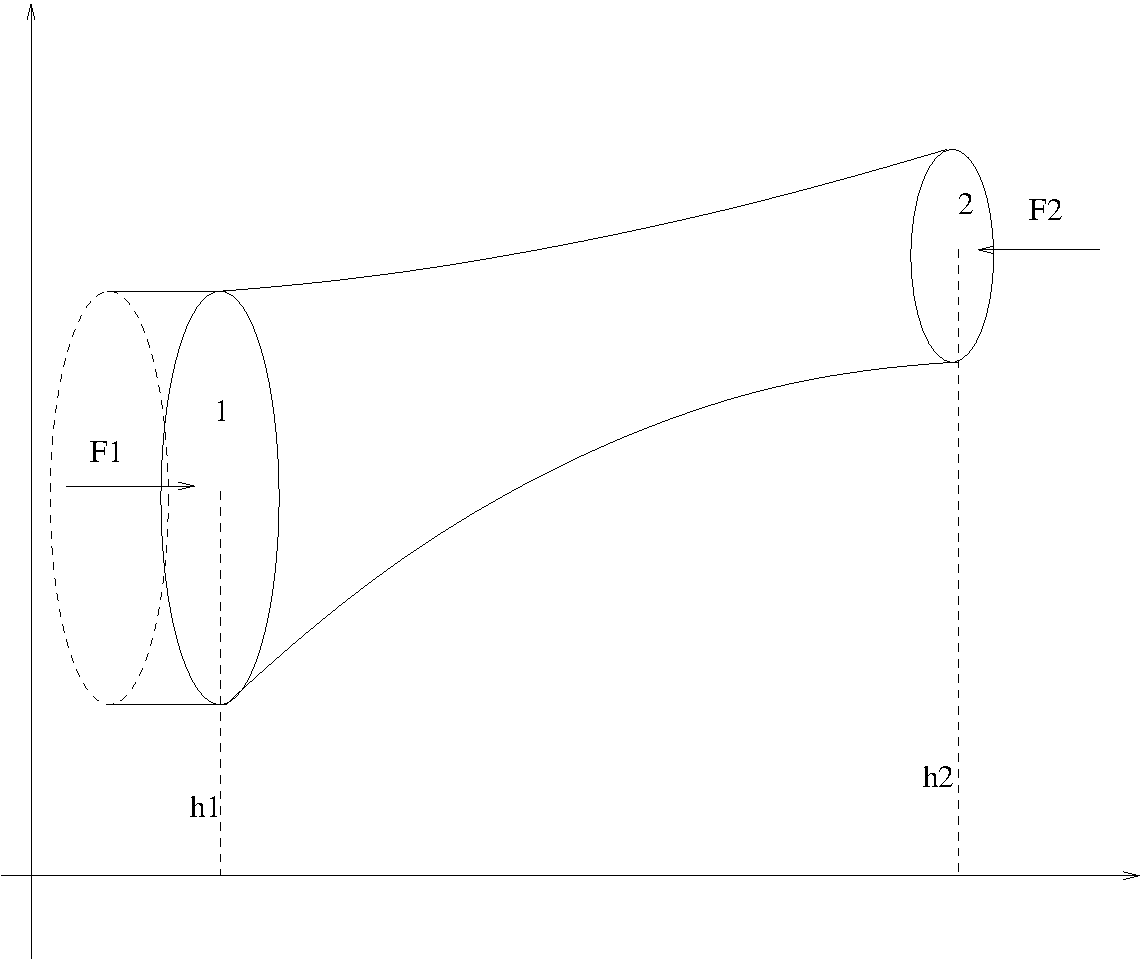
\includegraphics[scale=0.4]{immagini/fisica1/Bernoulli}
\end{center}
Consideriamo un tempo $\Delta t$ piccolo e una porzione di massa $\Delta m$. L'effetto netto tra la situazione iniziale e quella finale è di spostare l'elementino da un'estremità all'altro.

Il lavoro è svolto dalla forze esterne: $\ve F_1, \ve F_2, \ve P$ è $L=\Delta K$ poiché non c'è variazione di energia potenziale.
\[\Delta m=\rho \Delta V=\rho A_1 v_1\Delta t=\rho A_2 v_2 \Delta t\]
\[
\left\{
        \begin{array}{lll}
        L_1=F_1\Delta S_1=F_1v_1\Delta t=p_1A_1v_1\Delta t\\
        L_2=-F_2\Delta S_2=-F_2v_2\Delta t=-p_2A_2v_2\Delta t\\
        L_P=-\Delta mg(h_2-h_1)
        \end{array}
\right.
\]
\[\Delta K=\frac{1}{2}\Delta m(v_2^2-v_1^2)\]
\[L_1+L_2+L_P=\Delta K\]
\[p_1A_1v_1\Delta t-p_2A_2v_2\Delta t-\Delta mg(h_2-h_1)=\frac{1}{2}\Delta m(v_2^2-v_1^2)\]
\begin{align*}
&\Delta m\left[\left(gh_1-gh_2\right)+\frac{p_1A_1v_1\Delta t}{\Delta m}-\frac{p_2A_2v_2\Delta t}{\Delta m}\right]\\
=&\Delta m\left[\left(gh_1-gh_2\right)+\frac{p_1A_1v_1\Delta t}{\rho A_1v_1\Delta t}-\frac{p_2A_2v_2\Delta t}{\rho A_2v_2\Delta t}\right]\\
=&\Delta m\left[gh_1-gh_2+\frac{p_1}{\rho}-\frac{p_2}{\rho}\right]=L\\
=&\Delta K=\frac{1}{2}\Delta m(v_2^2-v_1^2)
\end{align*}
\[gh_1-gh_2+\frac{p_1}{\rho}-\frac{p_2}{\rho}=\frac{1}{2}(v_2^2-v_1^2)\]
\[gh_1+\frac{p_1}{\rho}+\frac{1}{2}v_1^2=gh_2+\frac{p_2}{\rho}+\frac{1}{2}v_2^2\]
\begin{Teo}[Bernoulli]
 Per un flusso laminare, incomprimibile, non viscoso e irrotazionale vale:
 \begin{equation}
  \rho gh+p+\frac{1}{2}\rho v^2=\const
\end{equation}
\end{Teo}
Nel caso che $v=0$ l'unico termine che sopravvive è quello che è chiamato \index{pressione!statica}pressione statica: $p+\rho gh$ in quanto è presente anche quando il fluido è fermo. L'altro termine invece è presente da solo se il fluido scorre in orizzonatale, quindi $\frac{1}{2}\rho v^2$ è detta \index{pressione!dinamica}pressione dinamica. In questo caso:
\[
 p_1+\frac{1}{2}\rho v_1^2=p_2+\frac{1}{2}\rho v_2^2=\const
\]
quindi si deduce che se la velocità è piccola la pressione è grande. Questo può essere spiegato anche usando l'equazione di continuità, infatti dove il tubo è più stretto la velocità è maggiore, questo significa che ci è stata un'accelerazione e quindi una forza dovuta ad una variazione di pressione che deve essere maggiore dove il tubo è più largo.

L'espressione del teorema di Bernoulli è molto simile alla conservazione dell'energia meccanica.
\[mgh+\frac{1}{2}mv^2=\const\]
\begin{Es}[ali di aereo]
L'aria sotto le ali di un aereo è più lenta di quella che passa sopra, quindi dalla legge di Bernoulli, considerando l'altezza uguale:
\[p_\text{sopra}+\frac{1}{2}\rho v_\text{sopra}^2=p_\text{sotto}+\frac{1}{2}\rho v_\text{sotto}^2\]
quindi se $v_\text{sopra}>v_\text{sotto}$ allora $p_\text{sopra}<p_\text{sotto}$ e allora c'è una forza netta verso l'alto.

Un altro contributo viene dal fatto che l'aria è fatta deviare verso il basso e il per terzo principio della dinamica ci deve essere una forza uguale e contrario applicata sulle ali. Tutto questo contribuisce alla \index{portanza}portanza.
\end{Es}
\section{Viscosità\index{viscosità}\index{eta@$\eta$|see{viscosità}}}
\label{viscosita fisica1}
\begin{figure}[htbp]
\centering
\subfigure{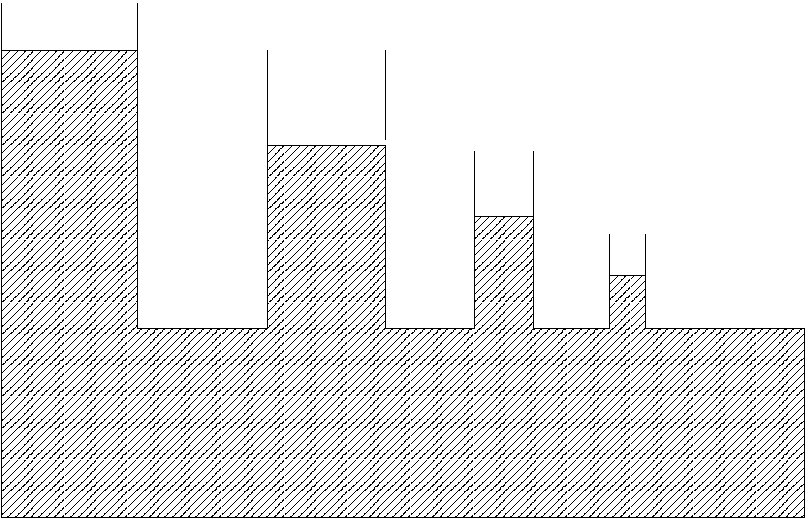
\includegraphics[scale=0.45]{immagini/fisica1/viscosita1}}\quad
\subfigure{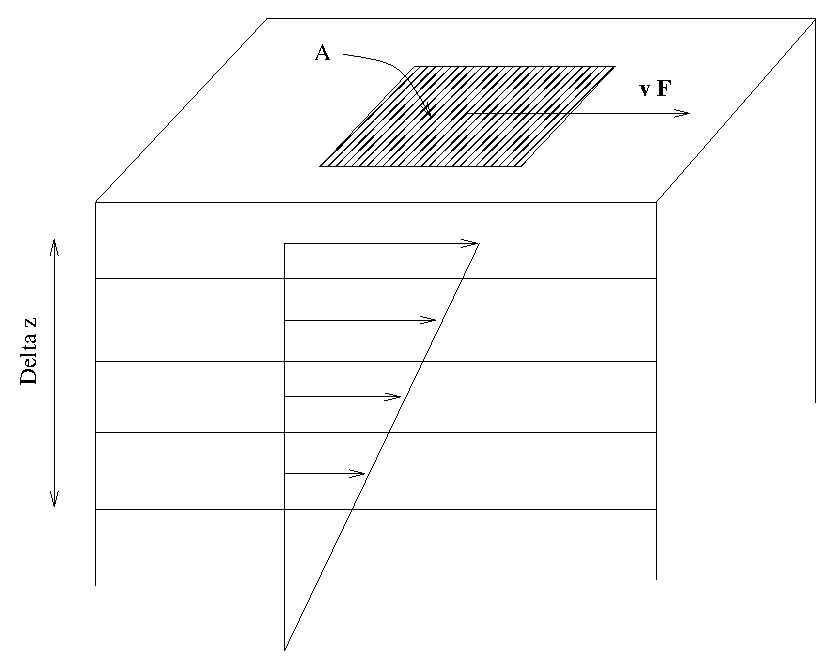
\includegraphics[scale=0.4]{immagini/fisica1/viscosita2}}
\caption{Perdita di pressione a causa della viscosità.}
\end{figure}

La pressione diminuisce, si ha una perdita di carico per un fluido viscoso a causa degli attriti interni. Siamo a regime laminare (velocità basse).


\[F=\eta A\frac{\ud v}{\ud z}\qquad\ve F=\eta A \ve\nabla v\qquad\eta=\text{coefficiente di viscosità}\]

\subsection{Legge di Poiseuille}

\vspace{0.4cm}
\begin{center}
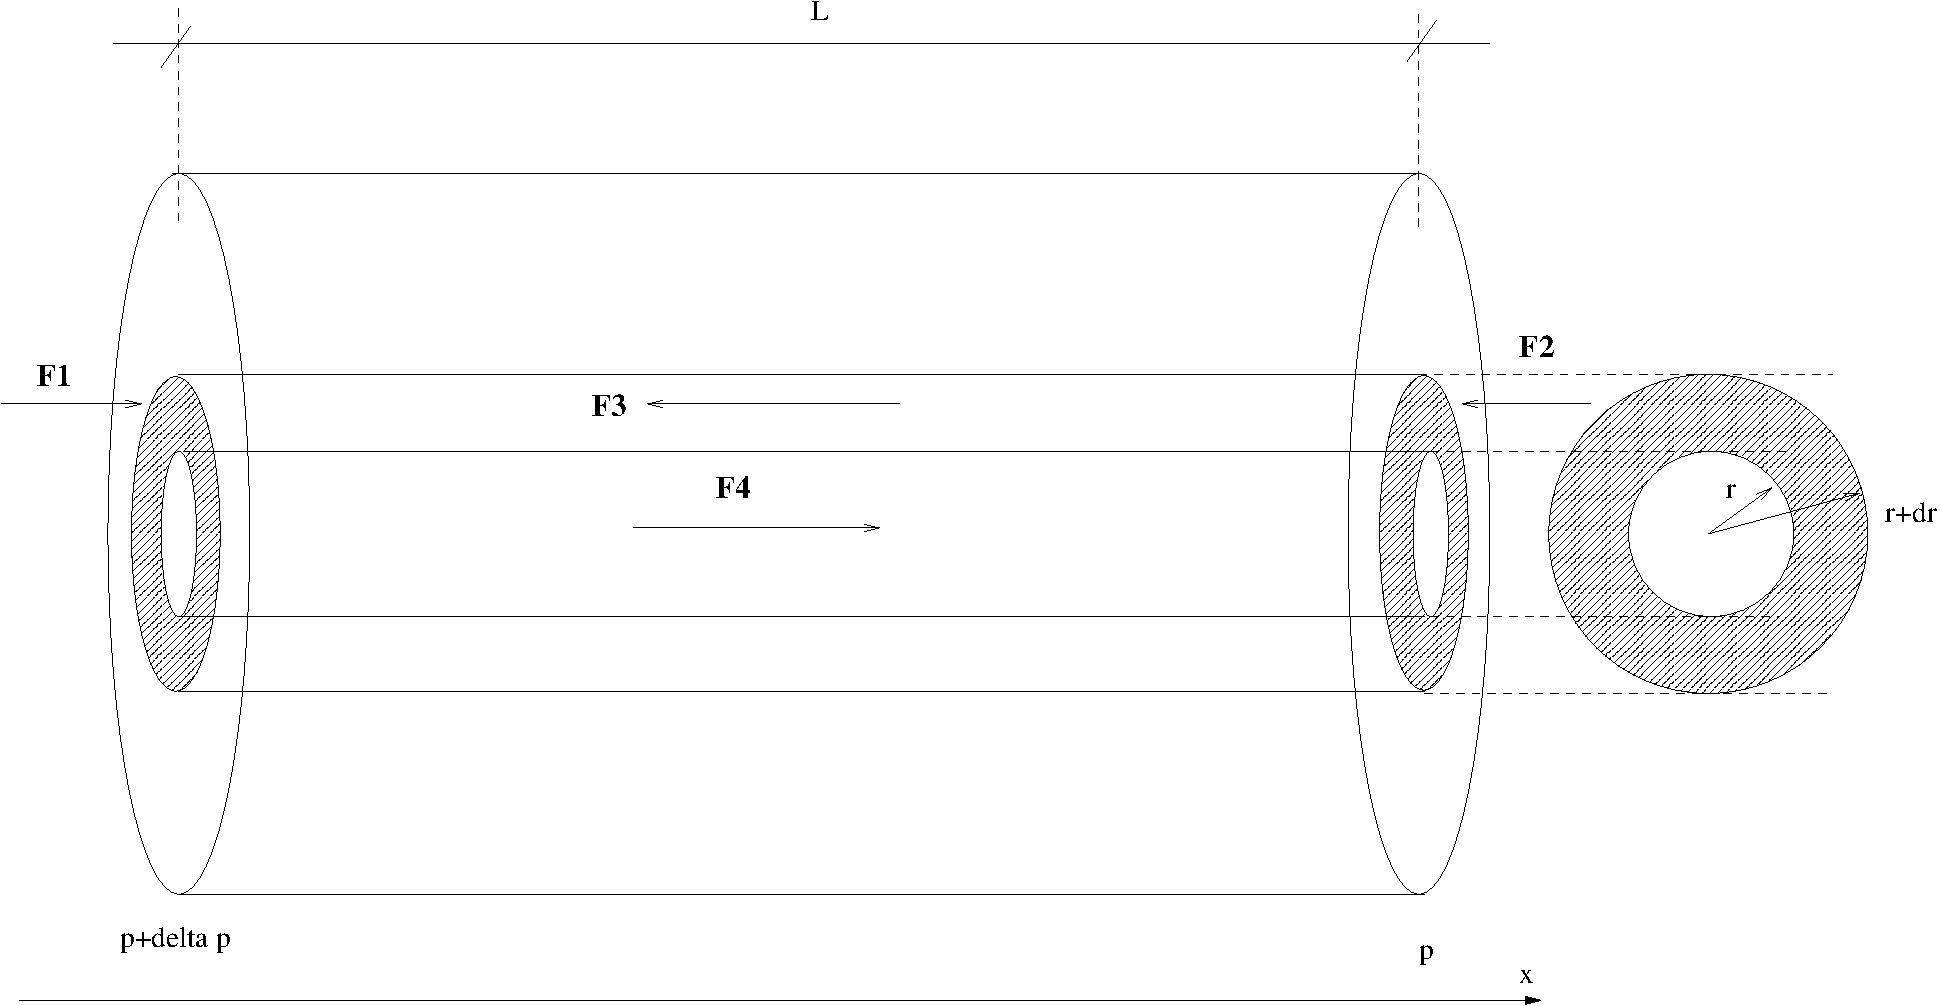
\includegraphics[scale=0.4]{immagini/fisica1/Poiseuille}
\end{center}


La velocità sarà massima al centro e minima ai bordi. Considero la porzione di fluido tra $r$ e $r+\ud r$. Le forze $F_3$ e $F_4$ sono dovute alle porzioni di fluido più esterne (più lente) e quelle più interne (più veloci).
\[F_1=(p+\Delta p)2\pi r\ud r\qquad F_2=-p2\pi r\ud r\]
\[F_3=L2\pi (r+\ud r)\eta\left. \frac{\ud v}{\ud r}\right|_{r+\ud r}\quad \frac{\ud v}{\ud r}<0\]
\[F_4=-L2\pi r\eta\left.\frac{\ud v}{\ud r}\right|_r\]
\[0=\sum F=(p+\Delta p)2\pi r\ud r-p 2\pi r\ud r+L 2\pi (r+\ud r)\eta\left.\frac{\ud v}{\ud r}\right|_{r+\ud r}\!\!\!\!\!\!\!\!\!\!-L2\pi r\eta\left.\frac{\ud v}{\ud r}\right|_r\]
\[\text{Taylor nell'intorno di $x=r$:\quad} \left.\frac{\ud v}{\ud r}\right|_x=\left.\frac{\ud v}{\ud r}\right|_r+\left.\frac{\ud^2 v}{\ud r^2}\right|_r(x-r)+\ldots\]


\[0=\Delta p r\ud r+\eta L\left\{(r+\ud r)\left.\frac{\ud v}{\ud r}\right|_{r+\ud r}\!\!\!\!\!\!\!\!\!\!-r\left.\frac{\ud v}{\ud r}\right|_r\right\}\simeq\]
\[\simeq\Delta p r\ud r+\eta L\left\{(r+\ud r)\left[\left.\frac{\ud v}{\ud r}\right|_r+\left.\frac{\ud^2 v}{\ud r^2}\right|_r\ud r\right]-r\left.\frac{\ud v}{\ud r}\right|_r\right\}=\]
\[=\Delta p r\ud r+\eta L\left\{r\frac{\ud v}{\ud r}+r\frac{\ud^2 v}{\ud r^2}\ud r+\ud r\frac{\ud v}{\ud r}+\frac{\ud^2 v}{\ud r^2}\ud r^2-r\frac{\ud v}{\ud r}\right\}\simeq\]
\[\simeq\Delta p r \ud r+\eta L\left[r\frac{\ud^2 v}{\ud r^2}\ud r+\frac{\ud v}{\ud r}\ud r\right]=0\]
\[\Delta p r+\eta L\left[r\frac{d^2 v}{\ud r^2}+\frac{\ud v}{\ud r}\right]=0\]
\[r\Delta p+\eta L\frac{\ud}{\ud r}\left(r \frac{\ud v}{\ud r}\right)=0\]
\[r\Delta p=-\eta L\frac{\ud}{\ud r}\left(r\frac{\ud v}{\ud r}\right)\]
\[\int_0^r r'\Delta p\,\ud r'=-\eta L\int_0^r\frac{\ud}{\ud r'}\left(r'\frac{\ud v}{\ud r'}\right)\ud r'\]
\[\Delta p\frac{1}{2}r^2=-\eta L r\frac{\ud v}{\ud r}\]
\[\Delta p\frac{1}{2}r=-\eta L \frac{\ud v}{\ud r}\]
\[\frac{\Delta p}{2}\int_R^r r'\,\ud r'=-\eta L\int_0^v \ud v'\]
\[\frac{\Delta p}{4}\left[r^2-R^2\right]=-\eta Lv\]
\[v=-\frac{\Delta p}{4}\frac{r^2-R^2}{\eta L}=\frac{\Delta p}{4\eta L}\left(R^2-r^2\right)\]
\begin{align*}
Q_v&=\int v \,\ud A=\int_0^R v(r)2\pi r\,\ud r=\int_0^R\frac{2\pi r\Delta p}{4\eta L}(R^2-r^2)\,\ud r\\
&=\frac{1}{2}\pi\int_0^R\frac{r\Delta p}{\eta L}\left(R^2-r^2\right)\ud r\\
&=\frac{\pi}{2}\frac{\Delta p}{\eta L}\int_0^R \left(rR^2-r^3\right)\ud r=\frac{\pi}{2}\frac{\Delta p}{\eta L}\left(\frac{R^4}{2}-\frac{R^4}{4}\right)\\
&=\frac{\pi\Delta p}{8\eta L}R^4
\end{align*}
  \begin{legge}[Poiseuille]
  \begin{equation}
    Q_v=\frac{\pi\Delta p}{8\eta L}R^4 
  \end{equation}
\end{legge}
si definisce una resisteza idraulica $\frac{8\eta L R^4}{\pi}$ in analogia con la resistenza elettrica.
\index{meccanica dei fluidi|)}


\chapter{Termodinamica\index{termodinamica|(}}
\minitoc
In meccanica è utile utilizzare ipotesi nelle quali ci siano pochi gradi di libertà, per esempio con i fluidi si usa l'approccio di Eulero. In termodinamica si considerano molte particelle e quindi molti gradi di libertà.

La termodinamica si occupa di scambi di energia e di cambiamento di stato di sistemi macroscopici, descritti da un numero piccolo di variabili macroscopiche come temperatura, volume e pressione. Si tratta sempre di sostanza pure e omogenee (una sola fase).

Una variabile di stato è una variabile\index{variabile!di stato} stazionaria(costante nel tempo), isotropa (uguale in tutte le direzioni), omogenea (uguale nello spazio).

Un sistema\index{sistema} è la porzione di materia sotto osservazione, l'ambiente \index{ambiente} tutto il resto. L'universo termodinamico\index{universo!termodinamico} è l'unione del sistema con l'ambiente. Un sistema aperto \index{sistema!aperto} scambia energia e materia con l'ambiente, un sistema chiuso \index{sistema!chiuso} scambia solo energia, un sistema isolato \index{sistema!isolato}non scambia né energia ne materia. Una parete adiabatica \index{parete!adiabatica}è una parete che non lascia passare calore, una diatermica \index{parete!diatermica}lascia passare calore.

Le variabili di stato vanno considerate dopo un certo tempo di rilassamento del sistema. La termodinamica classica si occupa dei sistemi all'equilibrio, analizza i sistemi prima e dopo le trasformazioni. Le trasformazioni \index{trasformazioni!quasistatiche}vengono considerate quasi statiche, cioè trasformazioni che passano attraverso infiniti stati di equilibrio in un tempo infinitamente lungo. Queste trasformazioni sono dette anche reversibili\index{trasformazioni!reversibili}.

Spesso vengono considerati l'equilibrio meccanico \index{equilibrio!meccanico}(nessun lavoro da e sul sistema), chimico \index{equilibrio!chimico}(nessuna reazione chimica interna), termico \index{equilibrio!termico}(nessuno scambio di calore).

\section{Principio zero della termodinamica\index{principio!zero della termodinamica}}
\begin{figure}[htbp]
\centering
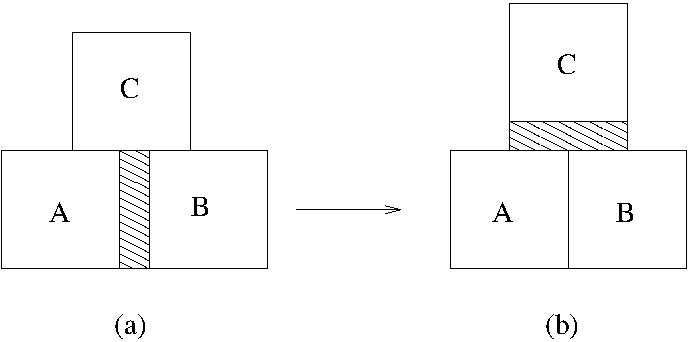
\includegraphics[scale=0.5]{immagini/fisica1/principio_zero}
\caption{(a)A e B scambiano calore con C, raggiungono l'equilibrio. (b) A e B non scambiano calore, sono all'equilibrio.}
\end{figure}
Il principio zero della termodinamica serve per definire il concetto di temperatura:
\begin{Pri}[principio zero della termodinamica]
Se due sistemi sono all'equilibrio termico con un terzo sistema allora sono all'equilibrio termico tra di loro.

Due sistemi hanno la stessa temperatura se sono in equilibrio termico. Due sistemi sono in equilibrio termico se messi a contatto le loro proprietà non cambiano.
\end{Pri}

\section{Temperatura\index{temperatura}}
\index{termometro}Il termometro è lo strumento per la misurazione della temperatura $T$. Per fare un termometro si sceglie una proprietà $X$ che varia in funzione di $T$. Se $X$ varia linearmente in funzione di $T$ allora (in kelvin):
\begin{equation}
T(X)=273.16\frac{X}{X_\text{triplo}}
\end{equation}
$X_\text{triplo}$ è il valore di $X$ al punto triplo dell'acqua ($\si{0.01}{\celsius}$). In questo modo la temperatura del punto triplo dell'acqua è di $\si{273.16}{\kelvin}$. Solitamente $X$ è il volume, la resistenza elettrica, la fem in una termocoppia, la pressione di un gas perfetto a volume costante\ldots I termometri empirici hanno problemi di non linearità e possono essere usati solo in piccoli intervalli dove si ritiene che il problema della non linearità possa essere trascurabile. Questi intervalli sono tutti intorni del punto triplo, in quanto al punto triplo dell'acqua per definizione tutti i termometri danno la stessa lettura. Il miglior termometro è quello a gas perfetto a volume costante.

\subsection{Termometro a gas perfetto a volume costante\index{termometro!a gas perfetto}}
Il termometro a gas perfetto è formato da un bulbo contenente un gas (perfetto, vedi~\ref{gas perfetto} a pag.\@ \pageref{gas perfetto}) che viene messo a contatto con il corpo di cui si vuole misurare la temperatura. Il gas tenderà ad espandersi o a contrarsi, cioè a cambiare il suo volume ma questo è mantenuto costate da una colonna di mercurio contenuta in un manometro collegato al bulbo. In questo modo si mantiene il volume costate e si legge il valore di pressione. La pressione per mantenere il volume costate è variata alzando o abbassando il serbatoio di mercurio del manometro. La temperatura empirica sarà proporzionale alla variazione di pressione del gas.

\section{Legge dei gas perfetti\index{legge!dei gas perfetti}}
\begin{legge}[Avogadro(1811)]
Uguali moli di gas, alla stessa pressione e temperatura contengono lo stesso numero $N_A$ di molecole, detto numero di Avogadro\index{Numero di!Avogadro}.
\end{legge}
Il numero di Avogadro vale circa $6.022\times 10^{23}$.
\begin{legge}[Boyle\index{Boyle}\index{legge!di Boyle}]
In una trasformazione a temperatura costate (isoterma):
\begin{equation}
p\propto\frac{1}{V}
\end{equation}
\end{legge}
\begin{legge}[Gay Lussac\index{legge!di Gay Lussac}\index{Gay Lussac}]
In una trasformazione a volume costante (isocora):
\begin{equation}
p\propto{T}
\end{equation}
\end{legge}
Il tutto si riassume nell'equazione dei gas perfetti\index{equazione! dei gas perfetti}:
\begin{equation}
pV=nRT=\frac{N}{N_A}RT=N\frac{R}{N_A}T=NkT
\end{equation}
con $R$ costante dei gas, $k=\frac{R}{N_A}$ costante di Boltzmann\index{costante! di Boltzmann}.
\section{Dilatazione termica\index{dilatazione termica}}
\subsection{Dilatazione termica dei solidi}
\subsubsection{lineare}
\begin{equation}
\Delta L=\alpha L_0\Delta T
\end{equation}
$\alpha$ dipendente dal tipo di materiale non è costante nella temperatura, ma spesso lo si può considerare tale. Altrimenti:
\begin{equation}
\Delta L=\int_{T_1}^{T_2} \alpha(T) L_0 \,\ud T
\end{equation}
Il coefficiente $\alpha$ è spesso isotropo, cioè uguali in tutte le direzioni. Quindi sviluppando con Taylor:
\[
 V_f = V_0(1+\alpha\Delta T)^3 \simeq V_0(1+3\alpha\Delta T)
\]
\begin{equation}
\Delta V=3\alpha V_0\Delta T
\end{equation}
\subsection{Dilatazione termica dei liquidi}
Nei liquidi non si può parlare di dilatazione lineare, quindi
\begin{equation}
\Delta V=\beta V_0\Delta T
\end{equation}
$\beta$ è abbastanza indipendente dalla temperatura, nei gas no, e si ricava dall'equazione dei gas perfetti.

\section{Teoria cinetica del gas perfetto\index{teoria cinetica del gas perfetto}}
\label{gas perfetto}
Un gas perfetto è una idealizzazione semplificativa, ma spesso adatta a descrivere gas reali (e non solo). Le ipotesi idealizzanti sono:
\begin{itemize}
\item il gas perfetto consiste di corpuscoli materiali, tutti uguali, in moto casuale e soggetti alle leggi del moto di Newton. Si può trattare sia di atomi singoli, sia di gruppi di atomi. In entrambi i casi li chiameremo molecole. Sono animate da moto in qualsiasi direzione e velocità comprese in un ampio intervallo;
\item il numero totale di molecole è straordinariamente grande. In questo modo si può applicare con ottimi risultati la statistica.
\item la somma dei volumi occupati da tutte le molecole è trascurabile rispetto al volume occupato dal gas;
\item se escludiamo gli effetti degli urti, sia tra molecole sia con le pareti, le molecole non sono soggette ad alcun'altra forza, in particolare non si considerano le forze intermolecolari;
\item gli urti sono perfettamente elastici e di durata trascurabile, quindi l'energia cinetica del sistema è costante. La durata trascurabile impone che l'energia potenziale totale delle molecole sia trascurabile.
\end{itemize}
\subsection{Pressione\index{pressione}}
Consideriamo $N$ molecole di un gas perfetto in un cubo di spigolo $L$. Prendiamo in considerazione una parete $A_1$. Una particella di velocità $\ve v$ e massa $m$ urta $A_1$:
\begin{equation}
\Delta p_x=-2mv_x
\end{equation}
è la variazione della quantità di moto nella direzione $x$, ortogonale ad $A_1$, della particella. Il tempo per andare e tornare è:
\begin{equation}
\Delta t=\frac{2L}{v_x}
\end{equation}
quindi ogni $\Delta t$ ci sarà un urto; se durante il tragitto la molecola dovesse incontrare una parete diversa, vi rimbarzerebbe senza mutare la componente $x$ della velocità né il tempo di percorrenza. Per l'impulso
\[
F_x\frac{2L}{v_x}=F_x\Delta t=\Delta p_x=-2mv_x
\]
\begin{equation}
F_x=-\frac{mv_x^2}{L}
\end{equation}
è la forza media (nel tempo) che la parete del recipiente applica sulla particella. Per il terzo principio della dinamica la particella sulla parere esercita una forza uguale e contraria, chiamiamola ancora $\ve F$ cambiando ora punto di vista, quello della particella:
\begin{equation}
F_x=\frac{mv_x^2}{L}
\end{equation}
La pressione $P_1$ su quella parete della particella è $\frac{\ve F\cdot \ve n}{A}=\frac{F_x}{A}$:
\begin{equation}
P_1=\frac{mv_x^2}{L^3}=\frac{mv_x^2}{V}
\end{equation}
Consideriamo ora il sistema di $N$ particelle, con velocità $\ve v_i$, la media dei quadrati delle velocità lungo $x$ è:
\begin{equation}
\media{v_x^2}=\frac{1}{N}\sum_{i=1}^{N}{v_{x_i}^2}
\end{equation}
analogamente per le altre componenti, che si sommano per dare $\media{v^2}=\media{v_x^2}+\media{v_y^2}+\media{v_z^2}$. Lo spazio è isotropo, quindi
\begin{equation}
\media{v_x^2}=\media{v_y^2}=\media{v_z^2}=\frac{1}{3}\media{v^2}
\end{equation}
La pressione media (facendo la media tra tutte le particelle) esercitata da una particella sulla parete $A_1$ è:
\[\media {P_{1}} = \frac{\sum P_{1i}}{N}=\frac{\sum m v_{xi}^2}{NV}=\frac{m\media{v_x^2}}{V}\]
Tutte le molecole eserciteranno una pressione media (facendo la media nel tempo) sulla parete $A_1$:
\begin{equation}
\media{P_x}=\frac{Nm\media{v_x^2}}{V}=\frac{1}{3}\frac{Nm\media{v^2}}{V}
\end{equation}
Il numero di molecole è così straordinariamente grande che la pressione sulla nostra parete non varia nel tempo, quindi $\media P=P$, allora:
\[P_x V=\frac{1}{3}Nm\media{v^2}\]
Ma la pressione è uguale su tutte le pareti, quindi:
\begin{equation}
PV=\frac{1}{3}mN\media {v^2}=\frac{1}{3}M\media{v^2}
\label{eq_gas_01}
\end{equation}
avendo introdotto $M=Nm$ la massa totale del gas. Introducendo la densità volumetrica $\rho=\frac{M}{V}$ la pressione:
\begin{equation}
P=\frac{1}{3}\rho\media{v^2}
\label{gas_pressione04}
\end{equation}
Questo risultato è stato ottenuto trascurando gli urti tra le molecole, ma risulta comunque valido. In caso di urto infatti le velocità di due molecole si scambiano e quindi ci il moto delle due molecole è semplicemente scambiato. Si noti che l'espressione precedente lega una grandezza microscopica (la velocità) ad una macroscopica (la pressione).
Usando invece l'energia cinetica del gas $K=\frac{1}{2}Nm\media{v^2}$ la \eqref{eq_gas_01} diventa:
\begin{equation}
pV=\frac{2}{3}K
\end{equation}
Introducendo la legge dei gas perfetti $pV=nRT$ si ricava:
\begin{equation}
 K = \frac{3}{2}nRT
\end{equation}
che lega la temperatura del gas alla sua energia interna.
\begin{Def}[velocità quadratica media]
\begin{equation}
v_{qm}=\sqrt{\media{v^2}}
\end{equation}
\end{Def}
Dalla \eqref{gas_pressione04} si ricava:
\begin{equation}
v_{qm}=\sqrt{\frac{3P}{\rho}}
\end{equation}
\begin{Es}[velocità delle molecole d'aria]
 Se la pressione atmosferica è \si{101000}{\pascal} e la densità dell'aria \si{1.2}{\kilo\gram\per\cubic\meter} la velocità quadratica media è:
 \[
  v_{qm}=\sqrt{\frac{3P}{\rho}}\simeq\si{500}{\meter\per\second}
 \]
questo non vuol dire che per fare un metro in linea retta una molecola ci mette $\Delta t \simeq \frac{\Delta s}{v_{qm}}=\frac{\si{1}{\meter}}{\si{500}{\meter\per\second}}=\si{2}{\milli\second}$ in quanto il suo percorso non è lineare, ma continua a variare direzione ad ogni urto.
\end{Es}
\subsubsection{Legge di Dalton}
In presenza di più gas diversi possiamo usare il fatto che il volume occupato dalle molecole è trascurabile rispetto al volume totale del gas. Quindi le loro pressioni si calcolano separatamente (\index{pressione!parziale} pressioni parziali):
\index{legge!di Dalton}
\begin{legge}[Dalton]
\begin{equation}
 p = \sum_i p_i = \frac{RT}{V}\sum_i{n_i}
\end{equation}
\end{legge}
La pressione parziale $i$--esima:
\begin{equation}
 p_i = \frac{RT}{V}n_i = \frac{nRT}{nV}n_i = p\frac{n_i}{\sum_i n_i} = pr_i
\end{equation}
dove $r_i$ è la frazione molare:
\begin{equation}
 r_i = \frac{n_i}{\sum_i n_i}
\end{equation}


\subsection{Libero cammino medio\index{libero cammino medio}}
\label{libero cammino medio fisica1}
Il libero cammino medio $\lambda$ è lo spazio medio in cui una particella non subisce urti con altra particelle. Supponiamo di avere molecole di diametro $d$. Avviene una interazione solo se i due centri delle molecole si avvicinano a una distanza inferiore a $d$. Si può pensare anche che la molecola considerata abbia diametro $2d$ e le altre siano puntiformi. Nel tempo $t$ la molecola spazza il volume di un cilindro di sezione $\pi d^2$ e di lunghezza $L_{cil}=vt$ con $v$ velocità della molecola. Supponiamo che il gas sia racchiuso in un volume $V$e contenga $N$ molecole. Il numero di molecole contenuto nel cilindro è quindi:
\[N_{\text{cil}}=N\frac{V_{\text{cil}}}{V}=N\frac{\pi d^2vt}{V}\]
Questo rappresenta anche il numero medio di urti nel tempo $t$ della molecola. Ad ogni urti la molecola cambia direzione, ma spazza sempre il volume di un cilindro analogo.

Il libero cammino medio è la distanza totale percorsa diviso il numero di urti subiti:
\[\lambda=\frac{L_{\text{cil}}}{N_{\text{cil}}}=vt\frac{V}{N\pi d^2vt}=\frac{V}{N\pi d^2}\]
Essendo $pV=NkT \Rightarrow V/N=kT/p$
\[\lambda=\frac{kT}{\pi d^2 p}\]
L'equazione è stata ricavata pensando che le molecole siano bersagli fermi. Le velocità semplificate non sono le stesse. Quella al numeratore è $\media{v}$ la velocità molecolare media misurata rispetto al recipiente che contiene il gas. Quella al denominatore rappresenta la velocità relativa media $v_\text{rel}$ rispetto alle altre molecole. Si può dimostrare (vedi \ref{calcolo_vel_rel_med}) che $v_\text{rel}=\media{v}\sqrt{2}$ e quindi:
\[\lambda=\frac{kT}{\sqrt{2}\pi d^2p}\]
Bisogna tenere anche conto che al di sotto di una certa pressione il libero cammino medio eccede le dimensioni del contenitore e il concetto stesso di libero cammino  medio perde di significato, in quanto è più probabile che la molecole incontri le pareti del recipiente piuttosto che altre molecole.

\subsection{Distribuzione delle velocità\index{distribuzione!delle velocità}}
Distribuzione di Maxwell delle velocità:\index{Maxwell}
\begin{equation}
N(v)=4\pi N\left(\frac{m}{2\pi kT}\right)^{\frac{3}{2}}v^2e^{-\frac{mv^2}{2kT}}
\end{equation}
con $m$ massa di una molecola, $M=N_Am$ massa molare.
$N(v)\ud v=$ numero di molecole con velocità compresa tra $v$ e $v+\ud v$, la velocità può essere solo positiva. Il numero totale di molecole:
\begin{equation}
N=\int_0^\infty N(v)\ud v
\end{equation}
Al crescere della temperatura la velocità media delle molecole aumenta e la curva si allarga; essendo il numero delle molecole costante, anche l'area lo è e quindi la curva si appiattisce.

\subsubsection{Velocità più probabile\index{velocità!più probabile}}
\begin{figure}[htbp]
\centering
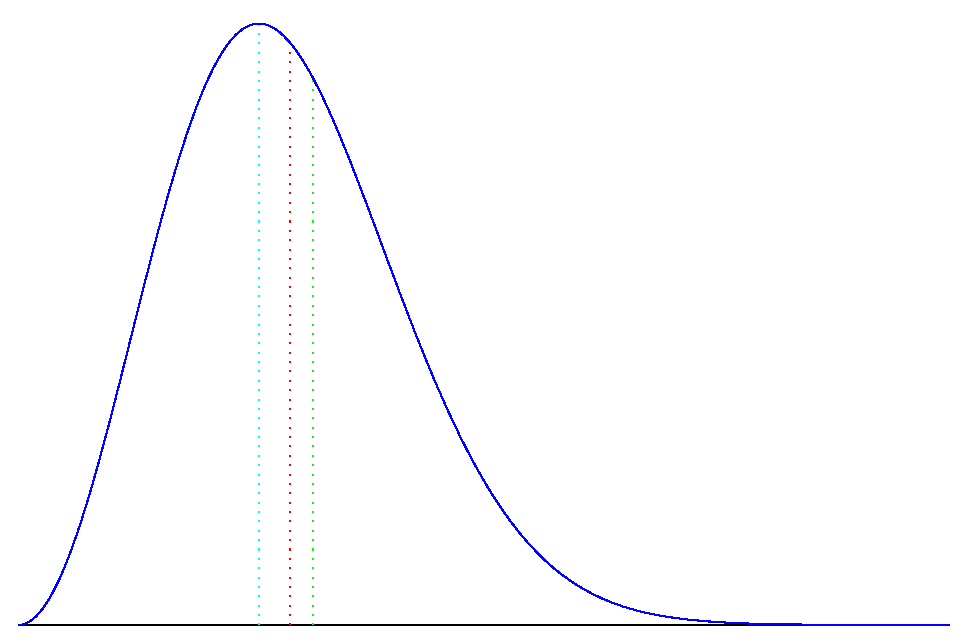
\includegraphics[scale=0.5]{immagini/fisica1/maxwell}
\caption{Distribuzione di Maxwell; velocità più probabile(blu), velocità media(rossa), velocità quadratica media(verde).}
\end{figure}
La velocità più probabile è quella in corrispondenza della quale la distribuzione ha un massimo, quindi:
\[4\pi N\frac{\ud}{\ud v}\left(\frac{m}{2\pi kT}\right)^{\frac{3}{2}}v^2e^{-\frac{mv^2}{2kT}}=0\]
\[2ve^{-\frac{mv^2}{2kT}}-\frac{v^3m}{kT}e^{-\frac{mv^2}{2kT}}=0\]
\[e^{-\frac{mv^2}{2kT}}v\left(2-v^2\frac{m}{kT}\right)=0\]
\begin{equation}
v_p=\sqrt\frac{2kT}{m}=\sqrt\frac{2RT}{M}
\end{equation}
Usando la velocità più probabile la distribuzione di Maxwell può essere scritta come:
\begin{equation}
 N(v) = \frac{4}{\sqrt{\pi}v_p^3}N v^2 e^{-v^2/v_p^2}
\end{equation}
\subsubsection{Velocità media\index{velocità!media}}
\begin{equation}
\media{v}=\frac{1}{N}\int_0^\infty vN(v)\ud v=\sqrt\frac{8kT}{\pi m}
\end{equation}

\subsubsection{Velocità quadratica media\index{velocità!quadratica media}}
\begin{equation}
\media{v^2}=\frac{1}{N}\int_0^\infty v^2N(v)\ud v=\frac{3kT}{m}
\end{equation}
\[v_\text{qm}=\sqrt{\media{v^2}}\]



\begin{figure}[htbp]
\centering
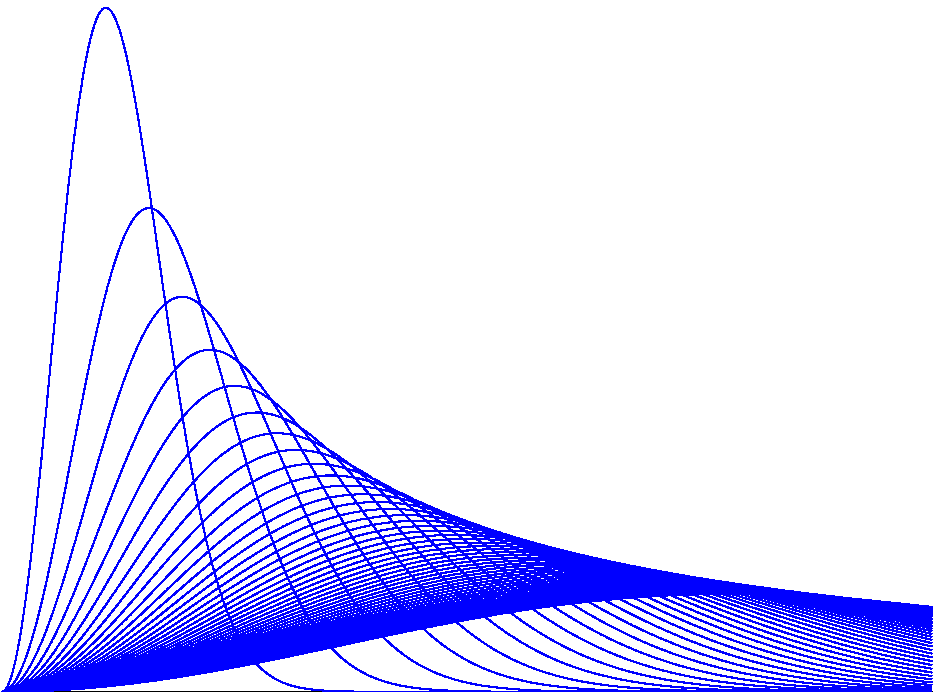
\includegraphics[scale=0.7]{immagini/fisica1/maxwell_famiglia2}
\caption{Famiglia di distribuzioni di Maxwell disegnate a intervalli costanti di temperatura.}
\end{figure}

\begin{figure}[htbp]
\centering
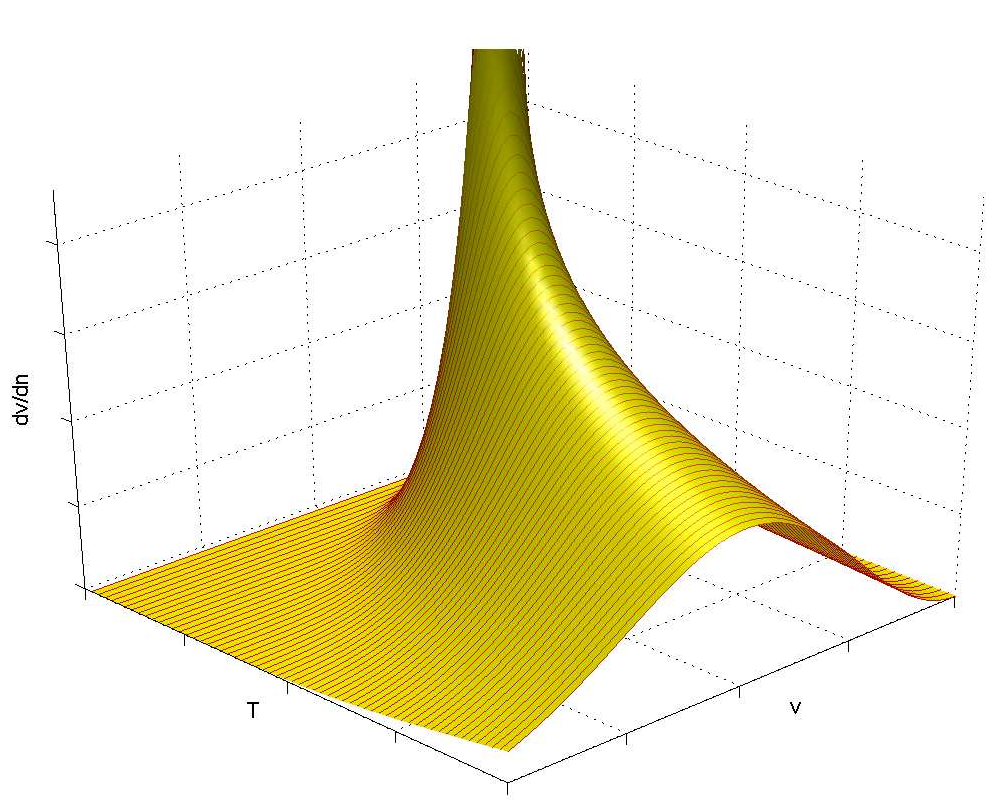
\includegraphics[scale=0.8]{immagini/fisica1/maxwell3d}
\caption{Andamento delle distribuzioni di Maxwell in funzione della temperatura.}
\end{figure}

\subsection{Distribuzione dell'energia\index{distribuzione!dell'energia}}
\begin{figure}[htbp]
\centering
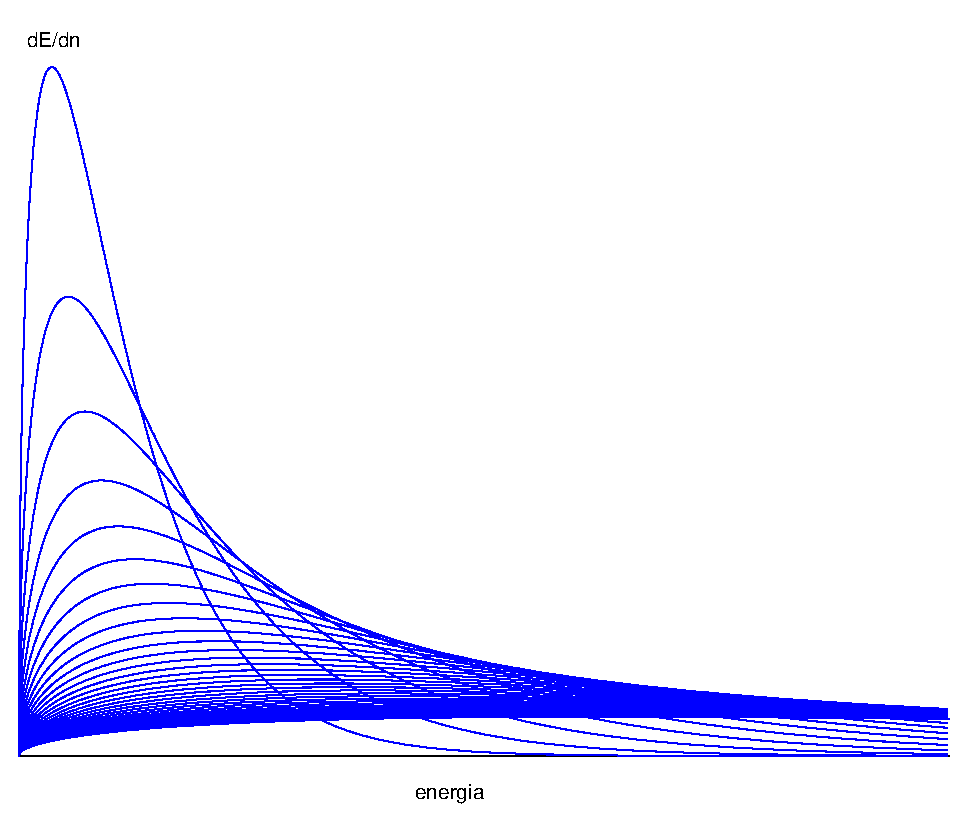
\includegraphics[scale=0.7]{immagini/fisica1/energia_max}
\caption{Famiglia di distribuzioni di energia disegnate a intervalli costati di temperatura.}
\end{figure}

Una molecola monoatomica di una gas ha solo energia cinetica $E=\frac{1}{2}mv^2$
\[v=\sqrt{\frac{2}{m}E}\]
Il numero di molecole che ha una certa velocità è uguale al numero di molecole che ha una certa energia:
\[N(E)\ud E=N(v)\ud v\]
\[N(E)=N(v)\frac{\ud v}{\ud E}=N(v)\sqrt\frac{2}{m}\frac{1}{2}E^{-\frac{1}{2}}\]
Distribuzione Maxwell--Boltzmann dell'energia:
\begin{equation}
N(E)=\frac{2N}{\sqrt{\pi}}\frac{1}{(kT)^{\frac{3}{2}}}\sqrt{E}e^{-\frac{E}{kT}}
\end{equation}
è indipendente dalla massa delle molecole, infatti un aumento di $m$ consegue una diminuzione di $v^2$ in modo che l'energia cinetica rimanga invariata.
\begin{figure}[htbp]
\centering
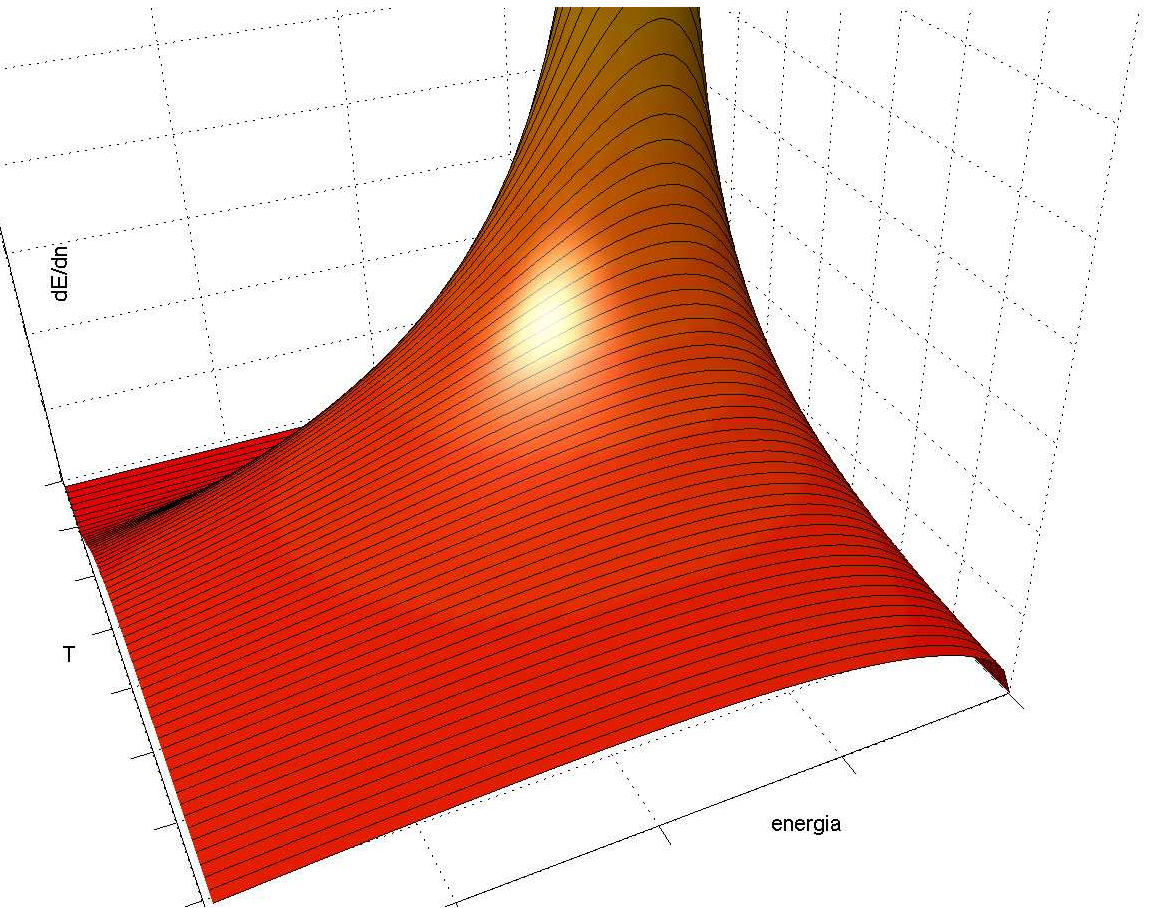
\includegraphics[scale=0.7]{immagini/fisica1/energia_max3d}
\caption{Andamento delle distribuzioni dell'energia in funzione della temperatura.}
\end{figure}

\subsubsection{Energia media\index{energia!media}}
Per un gas monoatomico
\begin{equation}
\media E=\frac{1}{N}\int_0^\infty E N(E)\ud E=\frac{3}{2}kT
\end{equation}
Per gli altri gas: $f$ numero di gradi di libertà
\begin{equation}
\media E=\frac{f}{2}kT
\end{equation}

\subsection{Riassunto teoria cinetica dei gas perfetti}
\begin{tabular}{lc}
massa molare&$M=N_A m$\\
pressione&$p=\frac{1}{3}\rho\media{v^2}$\\
velocità quadratica media&$v_\text{qm}=\sqrt\frac{3p}{\rho}=\sqrt\frac{3RT}{M}$\\
velocità più probabile&$v_p=\sqrt\frac{2RT}{M}$\\
velocità media&$\media{v}=\sqrt\frac{8RT}{\pi M}$\\
libero cammino medio&$\lambda=\frac{kT}{\sqrt{2}\pi d^2p}$\\
energia cinetica traslazionale \\per molecola monoatomica&$K=\frac{3}{2}kT$\\
\end{tabular}



\section{Trasferimenti di calore\index{trasferimento di calore}}
\subsection{Irraggiamento\index{irraggiamento}}
Ogni corpo emette radiazione elettromagnetica che dipende dalla temperatura. Leggi del corpo nero:
\begin{equation}P=\sigma T^4\qquad \lambda_\text{max}\sim\frac{1}{T}\end{equation}

\subsection{Conduzione\index{conduzione}}
Trasporto di calore senza trasporto di materia, è caratteristico dei solidi.
\begin{equation}
P=\frac{Q}{\Delta t}=K\frac{A}{\Delta x}\Delta T
\end{equation}
con $K$ coefficiente di conducibilità termica, $A$ l'area effettiva di contatto, $\Delta x$ lo spessore separatore.

\subsection{Convezione\index{convezione}}
Trasporto di calore con trasporto di materia, cioè con correnti convettive in movimento.


\section{Capacità termiche\index{capacità!termica}}
\begin{Def}[capacità termica]
Definiamo la capacita termica $C$ di un corpo la quantità di calore necessaria per far aumentare la sua temperatura di $\Delta T$:
\begin{equation}
C=\frac{Q}{\Delta T}
\end{equation}
\end{Def}
\begin{Def}[capacità termica specifica]
Definiamo la capacità termica specifica\index{capacità!termica!specifica} di una sostanza la quantità di calore necessaria per far aumentare  temperatura di $\Delta T$ un'unità di massa:
\begin{equation}
c=\frac{Q}{m\Delta T}=\frac{C}{m}
\end{equation}
\end{Def}
Esse non sono costanti, dipendono spesso dalla temperatura e dal tipo di trasformazione. Quindi al posto di $Q=mc\Delta T$ bisognerebbe scrivere:
\begin{equation}
Q=m\int_{T_0}^{T_f}c(T)\,\ud T
\end{equation}
conoscendo però come varia $c$ in funzione di $T$. Essendo $c$ variabile dal tipo di trasformazione per i gas si parla di $c_V$ calore specifico a volume costante e $c_p$ calore specifico a pressione costante.
\begin{Def}[calore specifico molare]
Il calore specifico molare è definito come\index{capacità!termica!molare}\index{calore specifico}:
\begin{equation}
c^{\text{mol}}=\frac{Q}{\Delta T n}=\frac{Q}{\Delta T}\frac{M}{m}=cM
\end{equation}
con $M=\frac{m}{n}$ massa molare\index{massa!molare}, $n$ numero di moli. Spesso $c^{\text{mol}}$ è indicato semplicemente con $c$.
\end{Def}

\index{Doulong}\index{Petit}Doulong e Petit osservarono che il calore specifico molare o capacità termica molare è uguale per tutti i solidi è circa $\si{25}{\joule\per\mole\per\kelvin}$. In realtà questo è il valore limite a cui tendono i solidi per temperature alte. Per temperature tendenti allo zero assoluto la capacità termica molare dei solidi tende a zero.


\section{Energia interna\index{energia!interna}}
L'energia interna di un gas perfetto è data solo dall'energia cinetica in quanto si è supposto che non ci sia energia potenziale. Per una molecola monoatomica $K=\frac{3}{2}kT$, per $n$ moli $E=K_n=nN_A\frac{3}{2}kT=\frac{3}{2}nRT$. Le molecole non puntiformi hanno anche energia cinetica rotazionale. Una molecola che possa ruotare su tutti i tre assi ha energia interna:
\[E=K=\frac{1}{2}mv_x^2+\frac{1}{2}mv_y^2+\frac{1}{2}mv_z^2+\frac{1}{2}I_x\omega_x^2+\frac{1}{2}I_y\omega_y^2+\frac{1}{2}I_z\omega_z^2\]
La molecola ha quindi 6 gradi di libertà, 3 traslatori e 3 rotazionali. Una molecola monoatomica ha solo 3 gradi traslatori e nessuno rotazionale in quanto essendo puntiforme $I=0$, una molecola biatomica ha 5 gradi di libertà.
\subsection{Principio di equipartizione dell'energia\index{principio!di equipartizione!dell'energia}}
Il principio di equipartizione dell'energia di Maxwell\index{Maxwell} dice che mediamente l'energia si ripartisce in modo equo tra i gradi di libertà. Ogni grado di libertà riceve $\frac{1}{2}kT$ di energia.
\begin{Pri}[equipartizione dell'energia]
\begin{equation}
E=\frac{f}{2}nRT
\label{equipartizione_00}
\end{equation}
con $f$ il numero di gradi di libertà delle particelle.
\end{Pri}
Si deduce che l'energia interna di un gas dipende esclusivamente dalla temperatura.
\subsection{Calore specifico molare dei solidi\index{capacità!termica!dei solidi}\index{calore specifico!dei solidi}}
Gli atomi dei solidi sono disposti secondo strutture reticolari e possono vibrare intorno alle loro posizioni di equilibrio in tre direzioni. Ogni atomo dispone anche di energia potenziale, quindi altri tre gradi di libertà. Avendo in totale 6 gradi di libertà dall'equazione \eqref{equipartizione_00} si ha:
\[E=3nRT\]
Se forniamo $Q$ calore al solido esso si trasformerà tutto in energia interna non compiendo il solido alcun lavoro:
\[Q=\Delta E=3nR\Delta T=nc\Delta T\]
\[c=\frac{3nR\Delta T}{n\Delta T}=3R\simeq \si{25}{\joule\per\mole\per\kelvin} \]
come previsto da Doulong\index{Doulong} e Petit\index{Petit}.
\subsection{Calore specifico dei gas\index{calore specifico!dei gas}\index{capacità!termica!dei gas}}
Come dimostrato più avanti in una trasformazione isocora tutto il calore si trasforma in variazione di energia interna in quanto non si compie lavoro.
\[c_V=\frac{Q}{n\Delta T}=\frac{\Delta E}{n\Delta T}=\frac{\frac{f}{2}nR\Delta T}{n\Delta T}=\frac{f}{2}R\]
\[c_p=c_V+R\quad\text{vedi relazione di Mayer \ref{mayer} pag.\pageref{mayer}}\]

\section{Primo principio della termodinamica\index{primo principio della termodinamica}\index{principio!primo della termodinamica}}
Consideriamo positivo qualsiasi cosa aumenti l'energia interna quindi consideriamo positivo il lavoro compiuto dall'ambiente sul sistema e positivo il calore ceduto dall'ambiente al sistema.
\[\Delta E=Q+L=E_f-E_i\]
con $E_f$, $E_i$ l'energia interna del sistema finale ed iniziale; $\Delta E$ dipende solo dalla situazione finale ed iniziale del sistema (per un gas solo dalla temperatura), quindi è una funzione di stato\index{funzione!di stato}, cioè una funzione che non dipende dalla particolare trasformazione, dal cammino percorso, ma solo dalle situazioni iniziali e finali. Mentre $L$ e $Q$ non sono funzioni di stato, la loro somma lo è. Questo è il primo principio della termodinamica:
\begin{Pri}[primo principio della termodinamica]
\begin{subequations}
\begin{equation}
Q+L=\Delta E
\end{equation}
considerando variazioni infinitesime diventa:
\begin{equation}
\delta Q+\delta L=\ud E
\end{equation}
\end{subequations}
$\ud E$ è un differenziale esatto essendo $E$ una funzione di stato.
\end{Pri}

\section{Trasformazioni di un gas\index{trasformazioni!di un gas}}
Le trasformazioni le possiamo dividere in due gruppi:
\begin{description}
\item[trasformazioni irreversibili]\index{trasformazioni!irreversibili} sono veloci, non sono determinate negli stati intermedi.
\item[trasformazioni quasistatiche]\index{trasformazioni!quasistatiche} sono lente, si dà il tempo al sistema di reagire attraversando infiniti stati di equilibrio intermedi. Una trasformazione quasi statica molto lenta idealizza una trasformazione reversibile, cioè una trasformazione che può tornare allo stato di partenza\index{trasformazioni!reversibili}.
\end{description}

\subsection{Calcolo del lavoro\index{lavoro!su un gas}}
Considerando una trasformazione reversibile e un gas perfetto:
\[\delta L=-F\ud x=-pA\ud x=-p\,\ud V\]
\begin{equation}
L=-\int_{V_0}^{V_f} p\,\ud V
\label{lavoro_gas02}
\end{equation}
Il modulo del lavoro è dunque, considerando il significato geometrico dell'integrale definito, l'area sottesa dalla curva $p=p(V)$. Il meno nella formula \eqref{lavoro_gas02} deriva dal fatto che considerando positivo il lavoro dell'ambiente la forza (dell'ambiente sul sistema) comprime il sistema, per esempio un contenitore con un pistone mobile, quindi lo spostamento è $-\ud x$, perché $x$ diminuisce.
\[\begin{array}{l}
L<0 \Leftrightarrow \text{espansione}\\
L>0 \Leftrightarrow \text{compressione}\\
\end{array}\]

In generale la forza di pressione non è una forza conservativa. Calcoliamo il lavoro svolto tra due condizioni termodinamiche, corrispondenti a due punti nel piano $pV$ attraverso due percorsi diversi (vedi figura~\ref{fig:forza_pressione}). Passiamo da $A$ a $D$ prima attraverso una isocora che faccia aumentare la pressione, da $A$ a $B$ e poi attraverso una isobara che faccia aumentare il volume, da $B$ a $D$. Il lavoro totale sarà la somma del lavoro lungo l'isocora $AB$ e dell'isobara $BD$. Il primo è nullo essendo la variazione di volume nulla. Il secondo è $\int_{V_i}^{V_f} p\ud V=p_f \Delta V$. Questo è anche il lavoro totale. Proviamo invece a calcolare il lavoro facendo prima una isobara e poi un'isocora. Il lavoro totale sarà: $p_i\Delta V$ diverso dal risultato precedente. Quindi la forza non è conservativa\footnote{se la forza fosse conservativa il lavoro in un ciclo sarebbe nullo e non sarebbe possibile realizzare le macchine termiche}.
\begin{figure}[htbp]
 \centering
% \input{immagini/fisica1/forza_pressione}
 \label{fig:forza_pressione}
\end{figure}

\subsubsection{Isobara $p=\const$}
\begin{equation}
L=-\int_{V_0}^{V_f} p\,\ud V=-p\Delta V
\end{equation}
\subsubsection{Isocora $V=\const$}
\begin{equation}
L=-\int_{V_0}^{V_f} p\,\ud V=0
\end{equation}
\subsubsection{Isoterma $T=\const$}
\begin{equation}
L=-\int_{V_0}^{V_f} p\,\ud V=-\int_{V_0}^{V_f} \frac{nRT}{V}\ud V=-nRT\int_{V_0}^{V_f} \frac{\ud V}{V}=-nRT\log\frac{V_f}{V_0}
\end{equation}
\subsubsection{Adiabatica $Q=0$}
\begin{equation}
L=\Delta E
\end{equation}
\subsection{Relazione di Mayer\index{Mayer}\index{relazione!di Mayer}}
\label{mayer}
Mostriamo la relazione tra $c_V$ e $c_p$. Consideriamo una trasformazione isocora e una isobara che partono dalla stessa situazione iniziale, e arrivano in configurazioni diverse, ma con la stessa temperatura:
\begin{figure}[htbp]
\centering
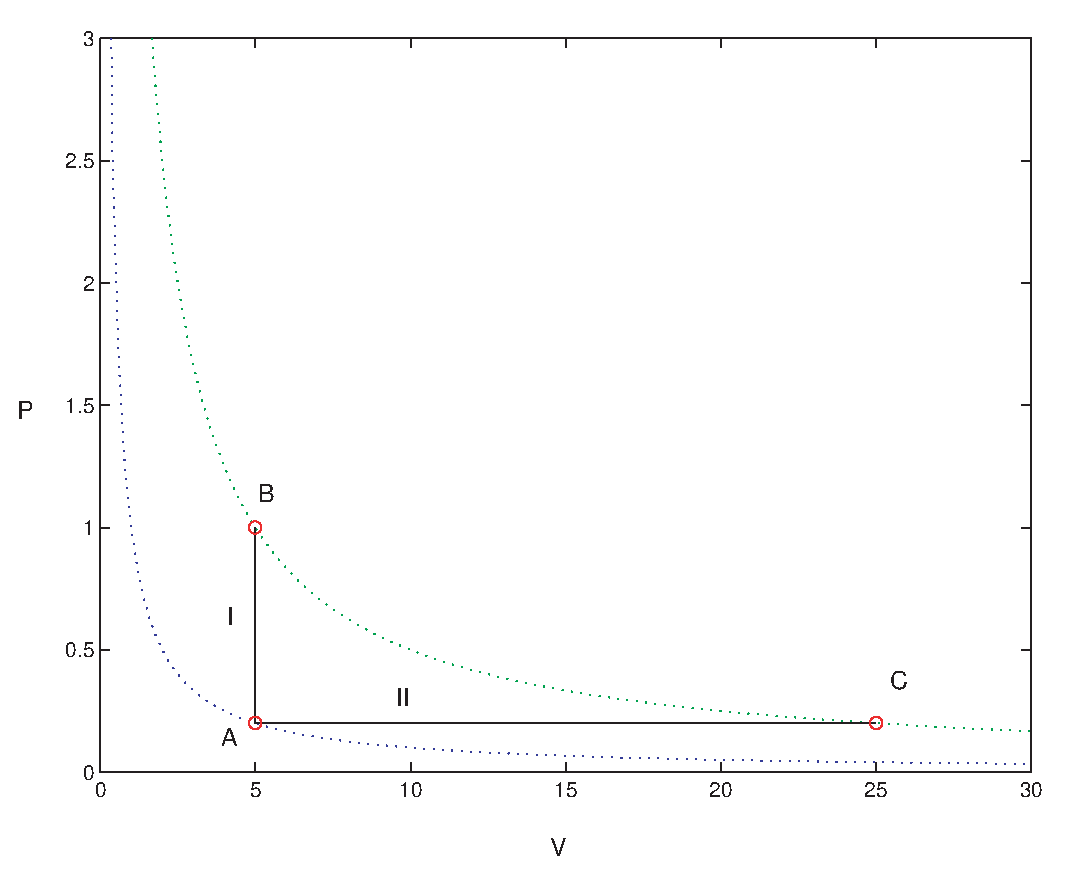
\includegraphics[scale=0.5]{immagini/fisica1/pV2_win}
\end{figure}
\begin{align*}
A\rightarrow B&\quad&V=\const&\quad&\text{I}\\
A\rightarrow C&\quad&p=\const&\quad&\text{II}
\end{align*}
\[\Delta E_I=Q_I+L_I=Q_I=nc_V\Delta T\]
\[\Delta E_{II}=Q_{II}+L_{II}=nc_p\Delta T-p\Delta V\]
$E_B=E_h$ perché $E$ dipende solo da $T$, quindi:
\[\Delta E_I=\Delta E_{II}\]
\[nc_V\Delta T=nc_p\Delta T-p\Delta V\]
\[nc_V\Delta T=nc_p\Delta T-nR\Delta T\]
\begin{Teo}[Relazione di Mayer]
 \begin{equation}
  c_p-c_V=R
 \end{equation}
\end{Teo}

\subsection{Adiabatiche}
\[Q=0\qquad \ud E=\delta Q+\delta L=\delta L=-p\ud V\]
per una isocora che lavora alle stesse temperature $\ud E=\delta Q=nc_V\ud T$
\[nc_V\ud T=-p\ud V=-\frac{nRT}{V}\ud V\]
\[c_V\ud T=-\frac{RT}{V}\ud V\]
\[\int_{T_i}^{T_f}\frac{c_V}{T}\,\ud T=-\int_{V_i}^{V_f}\frac{R}{V}\ud V\]
\[c_V\log\frac{T_f}{T_i}=-R\log\frac{V_f}{V_i}\]
\[R=c_p-c_V\qquad \gamma=\frac{c_p}{c_V}>1\]
\[\log\frac{T_f}{T_i}=\frac{c_V-c_p}{c_V}\log\frac{V_f}{V_i}=(1-\gamma)\log\frac{V_f}{V_i}\]
\[\log\frac{T_f}{T_i}=\log\left(\frac{V_f}{V_i}\right)^{\left(1-\gamma\right)}\]
\[\frac{T_f}{T_i}=\left(\frac{V_f}{V_i}\right)^{\left(1-\gamma\right)}\qquad T_fV_f^{\gamma-1}=T_iV_i^{\gamma-1}\qquad\]
\[TV^{\gamma-1}=\const\]
usando $PV=nRT$ e quindi $T=\const PV$:
\[PVV^{\gamma-1}=\const\]
\begin{equation}
PV^\gamma=\const\quad\text{Relazione di Poisson}
\end{equation}

\begin{Es}[Gradiente termico atmosferico]
L'aria è un cattivo conduttore termico, quindi quando delle masse d'aria a temperatura diversa si spostano si può considerare la trasformazione come adiabatica. La pressione atmosferica descresce con la quota, vedi \eqref{legge_atmosfera}. Per la legge di Archimede l'aria calda più leggera sale si espande a causa delle minore temperatura. Essendo la trasformazione adiabatica non c'è scambio di calore. Essendoci un'espansione la massa d'aria compie lavoro a scapito dell'energia interna, e quindi la temperatura diminuisce.

Per la legge di Stevino:
\[
 \ud P = -\rho g \ud h = -\frac{M}{V} g \ud h = -\frac{MP}{nRT} g \ud h
\]
dove abbiamo usato la legge dei gas perfetti ($PV=nRT$). Per le trasformazioni adiabatiche $TV^{\gamma-1}=\const$, allora $T^\gamma P^{1-\gamma} = \const$ e quindi possiamo collegare le variazioni di pressione alle variazioni di temperatura:
\[ T^{\gamma} P^{1-\gamma} = \const\]
\[ T = \const P^{\frac{\gamma - 1}{\gamma}}\]
\[ \log T = \frac{\gamma - 1}{\gamma} \log P + \const\]
\[\frac{1}{T}\frac{\ud T}{\ud P} = \frac{\gamma - 1}{\gamma} \frac{1}{P} \]
\[\frac{\ud T}{T} = \frac{\gamma - 1}{\gamma} \frac{\ud P}{P} \]
sostituendo:
\[
 \frac{\ud T}{\ud h} = -\frac{\gamma -1}{\gamma} \frac{Mg}{nR}
\]
Assumendo $\gamma = \frac{c_v+R}{c_v} = \frac{7}{5}$ (gas biatomico, $c_v = \frac{5}{2}R$) e la massa molare $\frac{M}{n} = \SI{28.88}{\gram\per\mol}$ si ottiene un gradiente costante:
\[
 \frac{\ud T}{\ud h} \simeq -\SI{9.74}{\kelvin\per\kilo\meter}
\]
questo gradiente è abbastanza più grande del grandiente osservato in quando si è trascurato la presenza di vapore acqueo che condensandosi al diminuire della temperatura sottrae calore sotto forma di calore latente.
\end{Es}


\subsection{Trasformazioni politropiche\index{trasformazioni!politropiche}}
Nelle trasformazioni politropiche $c$ è ritenuto costante.
\[\ud E=\delta Q+\delta L=nc\ud T-p\ud V\]
Il ragionamento è simile a quanto fatto con le adiabatiche; consideriamo una trasformazione isocora che lavora tra le stesse temperature $\ud E=nc_V\ud T$
\[nc\ud T-p\ud V=nc_V\ud T\]
\[nc\ud T-\frac{nRT}{V}\ud V=nc_V\ud T\]
\[(c_V-c)\ud T=-\frac{RT}{V}\ud V\quad \int_{T_0}^{T_f}\frac{c_V-c}{T}\ud T=-\int_{V_0}^{V_f}\frac{R}{V}\ud V\]
\[(c_V-c)\int_{T_0}^{T_f}\frac{\ud T}{T}=-R\int_{V_0}^{V_f}\frac{\ud V}{V}\]
\[\int_{T_0}^{T_f}\frac{\ud T}{T}=-\frac{c_p-c_V}{c_V-c}\int_{V_0}^{V_f}\frac{\ud V}{V}\]
\[\log\frac{T_f}{T_0}=-\frac{c_p-c_V}{c_V-c}\log\frac{V_f}{V_0}=\frac{c_p-c_V}{c_V-c}\log\frac{V_0}{V_f}\]
\[(k-1)=\frac{c_p-c_V}{c_V-c}\]
\[\log\frac{T_f}{T_0}=\log\left[\left(\frac{V_0}{V_f}\right)^{k-1}\right]\qquad\frac{T_f}{T_0}=\left(\frac{V_0}{V_f}\right)^{k-1}\]
\[T_fV_f^{k-1}=T_0V_0^{k-1}\qquad TV^{k-1}=\const\]
\[PVV^{k-1}=(nR)\const\qquad PV^k=\const\]
\[k=\frac{c_p-c}{c_V-c}\qquad c=\frac{kc_V-c_p}{k-1}\]
\subsubsection{Tutte le trasformazioni come politropiche}
\begin{center}
\begin{tabular}{l|ccc}
Isoterma&$pV=\const$&$k=1$&$c=\infty$\\
Isocora&$V=\const$&$k=\infty$&$c=c_V$\\
Isobara&$p=\const$&$k=0$&$c=c_p$\\
Adiabatica&$pV^\gamma=\const$&$k=\gamma>1$&$c=0$\\
\end{tabular}
\end{center}

\begin{figure}[htbp]
\centering
\subfigure[$c$ in funzione di $k$]{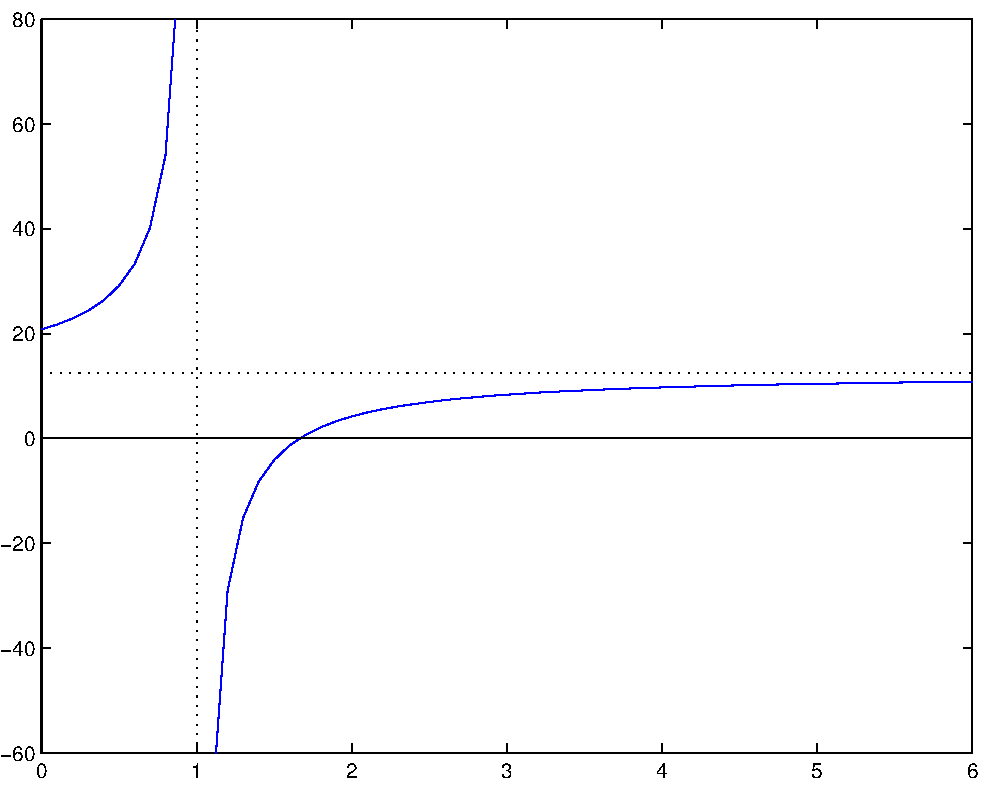
\includegraphics[scale=0.4]{immagini/fisica1/ck2}}
\subfigure[isoterma e adiabatiche in un grafico $p(V)$, quelle intermedie hanno \mbox{$c<0$}]{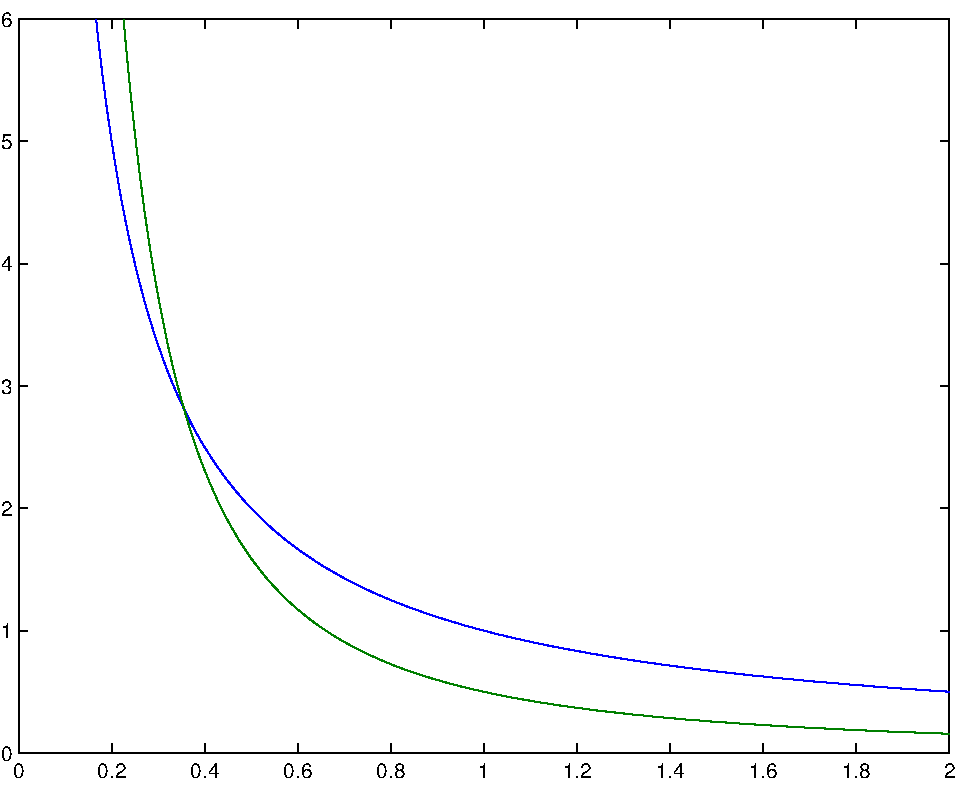
\includegraphics[scale=0.4]{immagini/fisica1/pvv2}}
\end{figure}

\begin{center}
\begin{tabular}{lccc}
&$L$&$Q$&$\Delta E$\\
\hline
Isoterma&$-nRT\log\frac{V_f}{V_0}$&$nRT\log\frac{V_f}{V_0}$&$nc_V\Delta T=0$\\
Isocora&$0$&$nc_V\Delta T$&$nc_V\Delta T$\\
Isobara&$-p\Delta V$&$nc_p\Delta T$&$nc_V\Delta T$\\
Adiabatica&$nc_V\Delta T$&$0$&$nc_V\Delta T$\\
\end{tabular}
\end{center}
\section{Entalpia}
\begin{Def}[Entalpia]
 \begin{equation}
  H = U + pV
 \end{equation}
\end{Def}
poiché $U$ è una funzione di stato e dipende solo dalla temperatura e il prodotto $pV=nRT$ dipende solo dalla temperatura, allora $H$ è una funzione di stato e dipende solo dalla temperatura.

L'entalpia è legata al calore specifico a pressione costante:
\begin{equation}
 \ud H = \ud U + \ud(nRT) = nc_v\ud T + nR\ud T = nc_p\ud T
\end{equation}
quindi in generale:
\begin{equation}
 \Delta H = n\int_{T_1}^{T_2} c_p\,\ud T
\end{equation}
o semplicemente
\begin{equation}
 \Delta H = nc_p\Delta T
\end{equation}
se $c_p$ è costante al variare della temperatura. Per una isobara vale dunque:
\begin{equation*}
 Q = n\int_{T_1}^{T_2} c_p\ud T = \Delta H
\end{equation*}
mentre per una isocora valeva:
\begin{equation*}
 Q = n\int_{T_1}^{T_2}c_v\ud T = \Delta U
\end{equation*}
quindi possiamo ridefinire i calori specifici molari come:
\begin{equation}
 c_v = \frac{1}{n}\frac{\ud U}{\ud T} \qquad c_p = \frac{1}{n}\frac{\ud H}{\ud T}
\end{equation}


\section{Trasformazioni cicliche\index{trasformazioni!cicliche}}
Una trasformazione ciclica è una trasformazione in cui gli stati iniziali e finali coincidono, quindi:
\begin{equation}
\Delta E=Q+L=0
\end{equation}
La macchine termiche trasformano il calore in lavoro e il loro ciclo è chiamo \index{ciclo!termico}ciclo termico. I frigoriferi trasformano il lavoro in trasferimento di calore, dalla sorgente più fredda a quella più calda e il loro ciclo è chiamato \index{ciclo!frigorifero}ciclo frigorifero.
\subsection{Ciclo di Carnot per un gas perfetto\index{Carnot}\index{ciclo!di Carnot}\index{macchina!di Carnot}}
\begin{figure}[htbp]
\centering
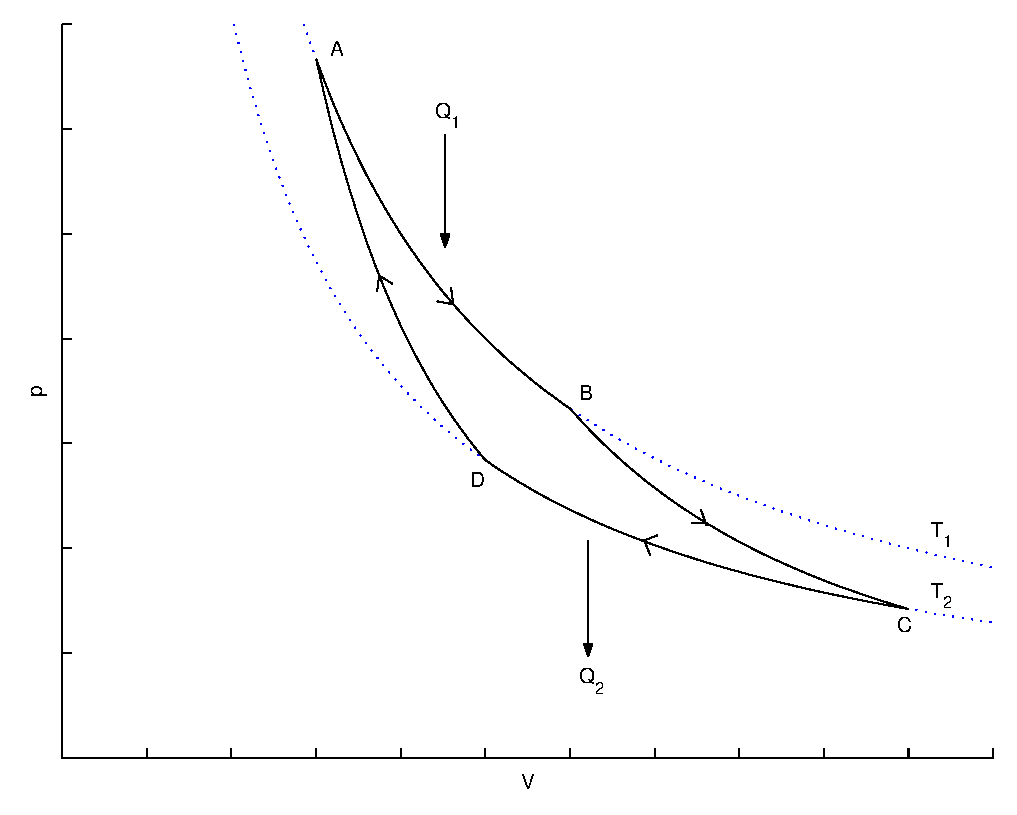
\includegraphics[scale=0.5]{immagini/fisica1/Carnot}
\caption{Ciclo di Carnot.}
\end{figure}
\parbox[]{\textwidth}{
\begin{enumerate}
\item Si porta il sistema alla temperatura $T_1$ immergendo in un bagno termico.
\item Il gas si espande da $V_A$ a $V_B$ seguendo una trasformazione isotermica.
\item Il gas si espande da $V_B$ a $V_C$ seguendo una trasformazione adiabatica.
\item Si porta il sistema alla temperatura $T_2$ immergendolo in un bagno termico.
\item Si comprime il gas da $V_C$ a $V_D$ seguendo una isoterma.
\item Si comprime il gas da $V_D$ a $V_A$ seguendo una adiabatica.
\end{enumerate}}
Nota: $Q_1>0$, $Q_2<0$, $L<0$

\[Q=Q_1-|Q_2|=-L\]
\[Q_2=nRT\log\frac{V_D}{V_C}\]
\[T_1V_B^{\gamma-1}=T_2V_C^{\gamma-1}\]
\[T_1V_A^{\gamma-1}=T_2V_D^{\gamma-1}\]
\[\left(\frac{V_B}{V_A}\right)^{\gamma-1}=\left(\frac{V_C}{V_D}\right)^{\gamma-1}\qquad \frac{V_B}{V_A}=\frac{V_C}{V_D}\]
Nella macchina di Carnot gli scambi di calore avvengono con delle isoterme, quindi i calori stanno alle temperature:
\begin{equation}
 \frac{|Q_2|}{Q_1}=\frac{nRT_2\log\frac{V_C}{V_D}}{nRT_1\log\frac{V_B}{V_A}}=\frac{T_2}{T_1}
\end{equation}

Il rendimento $\eta$ sarà maggiore quanto maggiore è il lavoro svolto dalla macchina sull'ambiente con minore scambio di calore.
\[\eta=\frac{|L|}{Q_1}=\frac{Q_1-|Q_2|}{Q_1}=1-\frac{|Q_2|}{Q_1}=1-\frac{T_2}{T_1}<1\]
La condizione migliore è quella della macchina perfetta \index{macchina!perfetta}in cui tutto il calore è trasformato in lavoro, $\eta_\text{perfetta}= 1$

\subsection{Frigorifero\index{frigorifero}\index{macchina!frigorifera}}
Si esegue il ciclo di Carnot al contrario. Si fornisce quindi lavoro e si ha un trasferimento di calore, trasferendolo dalla sorgente fredda a quella più calda.
Il coefficiente di merito sarà maggiore quando è maggiore il calore trasferito e minore il lavoro necessario.
Nota: $Q_1<0$, $Q_2>0$, $L>0$
\[0=L+Q=L+Q_2-|Q_1|\]
\[L=|Q_1|-Q_2\qquad\frac{Q_1}{Q_2}=\frac{T_1}{T_2}\]
\[\eta=\frac{Q_2}{L}=\frac{Q_2}{|Q_1|-Q_2}=\frac{T_2}{T_1-T_2}>0\]
Il frigorifero perfetto trasferisce calore dalla sorgente più fredda a quella più calda senza bisogno di lavoro, quindi $\eta\rightarrow\infty$

\subsection{Ciclo Otto\index{ciclo!Otto}}
Il ciclo Otto approssima molto il ciclo di un motore a benzina a quattro tempi.
\begin{itemize}
\item[] OA=aspirazione miscela
\item[] AB=compressione adiabatica
\item[] BC=accensione
\item[] CD=espansione adiabatica
\item[] DA=raffreddamento
\item[] OA=espulsione gas combusti
\end{itemize}

\[Q_{BC}=nc_V\Delta T=nc_V(T_C-T_B)>0\]
\[Q_{DA}=nc_V\Delta T=nc_V(T_A-T_D)<0\]
\[L+Q_{BC}-|Q_{DA}|=0 \qquad L=|Q_{DA}|-Q_{BC}<0\qquad |L|=Q_{BC}-|Q_{DA}|\]
\[\eta=\frac{|L|}{Q_{BC}}=\frac{Q_{BC}-|Q_{DA}|}{Q_{BC}}=1-\frac{|Q_{DA}|}{Q_{BC}}=1-\frac{nc_V(T_D-T_A)}{nc_V(T_C-T_B)}=1-\frac{T_D-T_A}{T_C-T_C}\]

Spesso il rendimento viene espresso in funzione del rapporto di compressione $r=\frac{V_2}{V_1}$
\[TV^{\gamma-1}=\const\]

\[\left\{
\begin{array}{l}
T_CV_1^{\gamma-1}=T_DV_2^{\gamma-1}\\
T_BV_1^{\gamma-1}=T_AV_2^{\gamma-1}\\
\end{array}\right.\]
\[(T_C-T_B)V_1^{\gamma-1}=(T_D-T_A)V_2^{\gamma-1}\]
\[\frac{T_D-T_A}{T_C-T_B}=\left(\frac{V_1}{V_2}\right)^{\gamma-1}\]

\[\eta=1-\frac{T_D-T_A}{T_C-T_B}=1-\left(\frac{V_1}{V_2}\right)^{\gamma-1}\!\!\!\!\!\!\!\!\! =1-\left(\frac{1}{r}\right)^{\gamma-1}\]

Più grande è $r$ più è grande $\eta$. Se $r$ è troppo grande $\Delta V$ è grande e nella compressione si crea troppo calore che provoca la preaccensione. Tipicamente $r=5$, quindi $\eta=0.55$. In realtà con questo rapporto di compressione nella macchine reali si ha $\eta=0.3$.

\subsection{Diagrammi di flusso}
I diagrammi di flusso sono degli schemi utili per descrivere le trasformazioni cicliche. I piani orizzontali rappresentano le fonti di calore a diversa temperatura, la sezione del tubo varia a seconda dell'energia interna del sistema.

\begin{figure}[!htbp]
\centering
\subfigure[ideale]{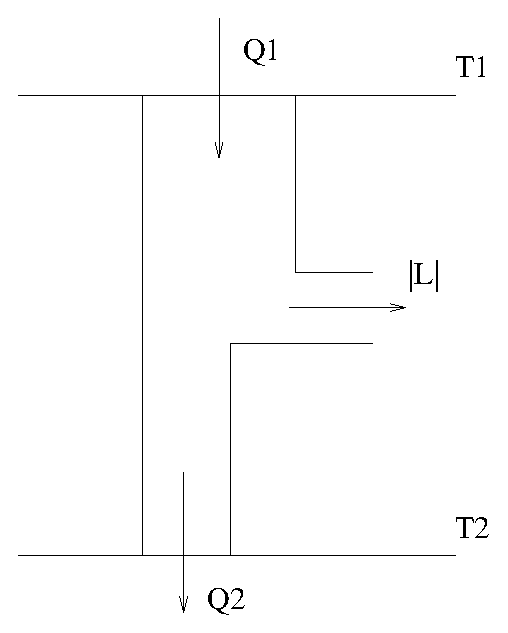
\includegraphics[scale=0.5]{immagini/fisica1/flusso_carnot}}\quad
\subfigure[perfetta]{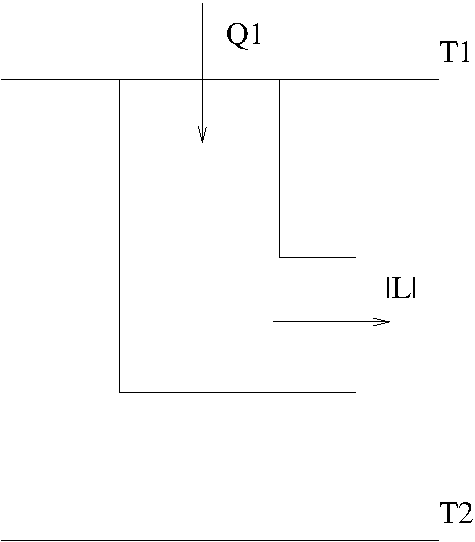
\includegraphics[scale=0.5]{immagini/fisica1/flusso_carnot_perf}}
\caption{Macchina di Carnot.}
\end{figure}
\begin{figure}[!htbp]
\centering
\subfigure[ideale]{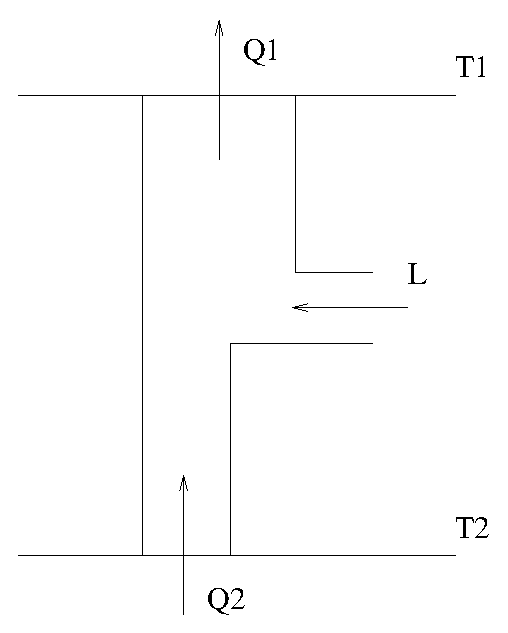
\includegraphics[scale=0.5]{immagini/fisica1/flusso_frigo}}\quad
\subfigure[perfetto]{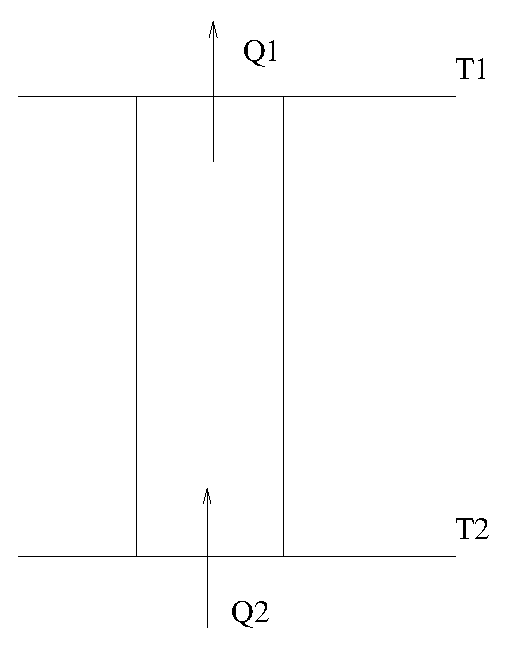
\includegraphics[scale=0.5]{immagini/fisica1/flusso_frigo_perf}}
\caption{Frigorifero.}
\end{figure}

\section{Secondo principio della termodinamica\index{secondo principio della termodinamica}\index{principio!secondo della termodinamica}}

\begin{Pri}[Enunciato di Kelvin]
\index{Kelvin}è impossibile realizzare una trasformazione il cui unico scopo è di produrre lavoro da una sola sorgente di calore.
\end{Pri}

\begin{Pri}[Enunciato di Clausius]
\index{Clausius}è impossibile realizzare una trasformazione il cui unico scopo sia quello di fare passare calore da una sorgente di bassa temperatura ad una più alta.
\end{Pri}

Una isoterma sembra violare Kelvin, in realtà trasforma tutto il calore in lavoro, ma non fa solo quello, infatti espande il gas.
\subsection{\texorpdfstring{$\text{Kelvin}\Leftrightarrow\text{Clausius}$}{Kelvin <=> Clausius}}

Chiamiamo $\bar{K}$ antikelvin un ciclo che viola Kelvin e $\bar{C}$ anticlausius un ciclo che viola Clausius. Dimostriamo che $\exists\bar{K}\Rightarrow\exists\bar{C}$ Sommiamo un antikelvin con un frigorifero e otteniamo un anticlausius (Figura \ref{CK1}). Quindi l'esistenza di un antikelvin implica l'esistenza di un anticlausius. Dopodiché $\nexists\bar{C}\Rightarrow\nexists\bar{K}$.

Sommando un anticlausius e una macchina termica e otteniamo un antikelvin (Figura \ref{CK2}), quindi
 $\exists\bar{C}\Rightarrow\exists\bar{K}$ e allora $\nexists\bar{K}\Rightarrow\nexists\bar{C}$. In definitiva abbiamo dimostrato che l'enunciato di Clausius e di Kelvin sono equivalenti.
\begin{figure}[htbp]
\centering
\includegraphics[scale=0.5]{immagini/fisica1/AK+Frigo}
\caption{Antikelvin più un frigorifero.}
\label{CK1}
\end{figure}

\begin{figure}[htbp]
\centering
\includegraphics[scale=0.5]{immagini/fisica1/AC+Carnot}
\caption{Anticlausius più una macchina termica.}
\label{CK2}
\end{figure}

\subsection{Teorema di Carnot\index{teorema!di Carnot}}
\begin{Teo}[Carnot: il più bravo sono io]
a parità di temperature non esiste macchina con rendimento migliore di quella di Carnot: $\eta_M\leq\eta_C$.
\end{Teo}
\subsubsection{Dimostrazione caso con due sorgenti}
Per assurdo: $\exists M: \eta_M>\eta_C$. Con la macchina di Carnot posso variare a piacimento il lavoro tenendo fisso $\eta$ allungando le isoterme. Scelgo una macchina di Carnot tale che $L_C=L_M$. Le macchine lavorano alle stesse temperature per ipotesi. La macchina $M$ avendo maggior rendimento avrà bisogno di meno calore, infatti:
\[\eta_M=\frac{|L_M|}{Q_M}>\eta_C=\frac{|L_C|}{Q_C}=\frac{|L_M|}{Q_C}\]
\[\frac{|L_M|}{Q_M}>\frac{|L_M|}{Q_C} \qquad Q_M<Q_C\]

Combino la macchina $M$ con la macchina di Carnot fatta funzionare al contrario, trovo un antikelvin. Assurdo, quindi: \[\eta_M\leq\eta_C\]
\begin{figure}[htbp]
\centering
\includegraphics[scale=0.5]{immagini/fisica1/M+c-1}
\caption{Macchina $M$ più la macchina di Carnot al contrario.}
\end{figure}

\begin{Cor}
Se la macchina è reversibile $\eta_M=\eta_C$. Per assurdo $\eta_M<\eta_C$, $M^{-1}+C=\bar{C},$ assurdo $\Rightarrow \eta_M\geq\eta_C\Rightarrow \eta_M=\eta_C$
\end{Cor}

Questo significa che tutte le macchine reversibili che lavorano tra due sorgenti $T_2 > T_1$: $\eta = 1-\frac{T_1}{T_2} = 1 - \frac{|Q_1|}{Q_2}$. Allora:
\begin{equation}
 \frac{Q_1}{T_2} + \frac{Q_2}{T_2} = 0
\end{equation}
il lavoro sarà:
\begin{equation}
 L = Q_2\eta = Q_2 \left(1 - \frac{T_1}{T_2}\right)
\end{equation}




\section{Entropia\index{entropia}}
Consideriamo una trasformazione reversibile per un gas perfetto:
\[\delta Q+\delta L=\ud E\qquad \delta Q-p\ud V=nc_V\ud T\]
\[\delta Q=nc_V\ud T+p\ud V\]
\[\frac{\delta Q}{T}\;\text{è un differenziale esatto?}\]
Per verificarlo integriamo la quantità e vediamo se si può esprime come differenza di funzioni che dipendono solo dallo stato iniziale e finale del sistema e non dalla particolare trasformazione. L'integrale quindi sarà una funzione di stato.
\begin{align*}
\int_i^f\frac{\delta Q}{T}&=\int_i^f\frac{nc_V\ud T+p\,\ud V}{T}=\int_{T_i}^{T_f}\frac{nc_V\ud T}{T}+\int_{V_i}^{V_f}\frac{p\,\ud V}{T}\\
&=nc_V\int_{T_i}^{T_f}\frac{\ud T}{T}+\int_{V_i}^{V_f}\frac{\frac{nRT}{V}\ud V}{T}=nc_V\int_{T_i}^{T_f}\frac{\ud T}{T}+nR\int_{V_i}^{V_f}\frac{\ud V}{V}\\
&=(nc_V\log T_f+nR\log V_f)-(nc_V\log T_i+nR\log V_i)=S_f-S_i\\&=\Delta S
\end{align*}
\[S=nc_V\log T+nR\log V+\const=\text{entropia}\]
\[\int_i^f\frac{\delta Q}{T}=\Delta S\qquad \oint\frac{\delta Q}{T}=0\]
L'entropia è una funzione di stato. La definizione data vale solo per trasformazioni reversibili. Per una trasformazione irreversibile si può calcolare $\Delta S$ usando una trasformazione reversibile che colleghi gli stessi stati iniziali e finali (vedi esempio espansione libera).
\subsubsection{Isocora}
\[\Delta S=nc_V\log\frac{T_f}{T_i}+nR\log\frac{V_f}{V_0}=nc_V\log\frac{T_f}{T_i}\]
\subsubsection{Isobara}
\[\frac{V_i}{V_f}=\frac{T_i}{T_f}\]
\begin{align*}
\Delta S=&nc_V\log\frac{T_f}{T_i}+nR\log\frac{V_f}{V_i}=nc_V\log\frac{T_f}{T_i}+nR\log\frac{T_f}{T_i}\\
=&\log\frac{T_f}{T_i}(c_V+R)=nc_p\log\frac{T_f}{T_i}
\end{align*}
\subsubsection{Adiabatica}
\[\delta Q=0 \Rightarrow \Delta S=0\]
Le adiabatiche vengono anche chiamate trasformazioni isoentropiche
\subsubsection{Isoterma}
\[\Delta S=nc_V\log\frac{T_f}{T_i}+nR\log\frac{V_f}{V_0}=nR\log\frac{V_f}{V_0}=\frac{Q}{T}\]
\subsubsection{Espansione libera}
L'espansione libera è una adiabatica irreversibile, quindi non si può concludere che $\Delta S=0$. Lo stato iniziale e quello finale sono alla stessa temperatura, quindi si trovano sulla stessa isoterma. La trasformazione pur non essendo isoterma ha $\Delta S$ di una isoterma. Se il volume finale è il doppio di quello iniziale:
\[\Delta S=nR\log\frac{V_f}{V_i}=nR\log 2\]

\subsection{Entropia nei cicli\index{entropia!nei cicli}}
Il teorema di Clausis estende il risultato a due sorgenti dal teorema di Carnot con macchine reversibili: $\frac{Q_1}{T_1} + \frac{Q_2}{T_2} = 0$.
\begin{Teo}[Clausius]
 Consideriamo macchina generica $M$ con $n$ sorgenti di calore a temperature diverse $T_i$ dalle quali assorbe calore $Q_i$. Allora vale:
  \begin{equation}
   \sum_i \frac{Q_i}{T_i} \leq 0
  \end{equation}
l'uguaglianza vale solo se la macchina è reversibile.
\end{Teo}

Per dimostrare il teorema introduciamo $n$ macchine reversibili $C_i$, ognuna che opera tra due sorgenti, $T_i$ e $T_0$. La macchina $M$ non scambia calore con $T_0$. Le macchine reversibili $C_i$ sono tali da scambiare lo stesso calore $Q_i$ dalla sorgente a temperatura $T_i$ come la macchina $M$, ma con segno opposto. Quindi se la macchina $M$ assorbe calore $|Q_i|$ alla sorgente a temperatura $T_i$ allora $C_i$ cede $|Q_i|$ e viceversa.

Usando la relazione generica $\frac{Q_A}{T_A} + \frac{Q_B}{T_B} = 0$ si ottiene alla macchina $C_i$:
\[
 Q_{i,0} = \frac{T_0}{T_i} Q_i
\]

Consideriamo ora la $H=\text{macchina infernale}=M+\sum_{i=1}^{n}C_i$ come in figura \ref{fig:hell_machine}. Poiché i calori della macchina $M$ e $C_i$ si compensano per ogni sorgente a temperatura $T_i$ il risultato netto è che $H$ scambia calore netto solo con la sorgente a $T_0$. Per il postulato di Kelvin questa macchina non può compiere lavoro, cioè $L_H \leq 0$ e quindi per il primo principio $Q_H = Q_0 \leq 0$, dove $Q_0 = \sum_{i=1}^n Q_{i,0}$ è il calore scambiato da $H$ con la sorgente a temperatura $T_0$. Allora:
\[
 Q_0 = \sum Q_{i,0} = T_0\sum_{i=1}^{n} \frac{Q_i}{T_i}\leq 0
\]
e quindi $\sum_{i=1}^n{Q_i}{T_i}\leq 0$.

\begin{figure}[htbp]
\centering
\includegraphics[scale=0.5]{immagini/fisica1/hell_machine}
\caption{macchina infernale}
\label{fig:hell_machine}
\end{figure}

passando a variabili continue:
\begin{equation}
\oint\frac{\delta Q}{T}\leq 0\quad\text{diseguaglianza di Clausius}
\label{clausius_dis}
\end{equation}
la disequazione vale per qualsiasi gas, per qualsiasi trasformazione.

Se $M$ reversibile costruisco $H'=M^{-1}+\sum_{i=1}^N C_i$, $Q$ è cambiato si segno, quindi la diseguaglianza diventa:
\[\oint\frac{\delta Q}{T}\geq0\]
Confrontando questa diseguaglianza con quella di Clausius \eqref{clausius_dis} si conclude che per una macchina reversibile:
\begin{equation}
\oint\frac{\delta Q}{T}=0
\end{equation}
Infatti considerando trasformazioni reversibili $\Delta S$ è una funzione di stato:
\[\int_i^f\frac{\delta Q}{T}=S(f)-S(i)\qquad\oint\frac{\delta Q}{T}=\int_A^A\frac{\delta Q}{T}=S(A)-S(A)=0\]

\subsection{Entropia per qualsiasi trasformazione\index{entropia! per qualsiasi trasformazione}}
Considerando un ciclo con trasformazioni irreversibili come in figura~\ref{fig:ciclo_misto}
\begin{figure}[!htbp]
\centering
\includegraphics[scale=0.5]{immagini/fisica1/ciclo_misto}
\label{fig:ciclo_misto}
\end{figure}
dalla diseguaglianza di Clausis $\oint\frac{\delta Q}{T}\leq 0$:
\[\underbrace{\int_i^f\frac{\delta Q}{T}}_\text{irreversibile}-\underbrace{\int_i^f\frac{\delta Q}{T}}_\text{reversibile}\leq 0\]
\[\underbrace{\int_i^f\frac{\delta Q}{T}}_\text{irreversibile}\leq\underbrace{\int_i^f\frac{\delta Q}{T}}_\text{reversibile}=\Delta S\]
Per una trasformazione qualsiasi (anche irreversibile):
\[\Delta S\geq\int_i^f\frac{\delta Q}{T}\]
Nel caso sia reversibile vale l'uguaglianza.

\subsection{Entropia e secondo principio}
\[\Delta S\geq\int_i^f\frac{\delta Q}{T}\]
se consideriamo un sistema isolato $\delta Q=0$ quindi
\begin{equation}
\Delta S\geq 0 
\end{equation}
Questa equazione è equivalente al secondo principio. Se avvengono solo trasformazioni reversibili $\Delta S=0$ quindi l'entropia dell'universo non può diminuire. Le trasformazioni reversibili si dice che non lasciano traccia entropica. L'aumento dell'entropia è equivalente al secondo principio (enunciato di Kelvin o di Clausius):
\subsubsection{Macchina perfetta\index{macchina!perfetta}}

\[\Delta S_\text{sistema}=0 \qquad\text{perché ciclo}\]
\[\Delta S_\text{universo}=\Delta S_\text{sistema}+\Delta S_\text{sorgente}\]
\[\Delta S_\text{universo}=\Delta S_\text{sorgente}=\frac{Q_1}{T_1}<0\]
\[\Delta S<0\qquad \text{impossibile}\]
$Q_1$ è negativo perché lo si deve considerare dal punto di vista della sorgente per calcolare la variazione di entropia della sorgente.

\subsubsection{Frigorifero perfetto\index{frigorifero!perfetto}}


\[|Q_1|=|Q_2|=Q\]
\[\Delta S_\text{universo}=\Delta S_\text{sistema}+\Delta S_1+\Delta S_2=\frac{|Q|}{T_1}-\frac{|Q|}{T_2}=|Q|\left(\frac{1}{T_1}-\frac{1}{T_2}\right)<0\]
\[\Delta S<0\qquad \text{impossibile}\]
questo perché $T_1>T_2$; se fosse $T_2>T_1$ cioè il calore circolasse dalla sorgente calda a quella fredda $\Delta S\geq 0$ e non ci sarebbe nulla di assurdo.

\subsubsection{Secondo principio\index{secondo principio della termodinamica}\index{principio!secondo della termodinamica}}
\[\Delta S_\text{sistema isolato}\geq 0\]
L'uguaglianza solo per trasformazioni reversibili.


\subsection{Interpretazione statistica dell'entropia}
\begin{figure}[htbp]
\centering
\includegraphics[scale=0.45]{immagini/fisica1/exp_Joule}
\caption{espansione di Joule.}
\end{figure}

Nell'espansione libera (o di Joule\footnote{si legge giul, non giaul (è francese!)}) si verifica sperimentalmente che la temperatura non varia. Essa è una trasformazione irreversibile spontanea. \`E isolata dall'ambiente essendo le pareti adiabatiche. Le pareti sono indeformabili, non viene compiuto lavoro. $\Delta S_\text{ambiente}=0$ $V_f=2V_i$

\[\Delta S_\text{universo}=\Delta S_\text{sistema}+\Delta S_\text{ambiente}=nR\log\frac{V_f}{V_i}=nR\log 2>0\]

\[P=\text{numero di microstati che danno luogo ad uno stato termodinamico}\]
$P$ è la probabilità che il sistema si configuri in un dato stato termodinamico a meno di un coefficiente, chiamata anche molteplicità.

$S$ è una variabile termodinamica estensiva, quindi per calcolare l'entropia del sistema si somma $S_1$ della parte sinistra e $S_2$ della parte destra. Le variabili termodinamiche come $T$, $p$ sono intensive e sommarle in questo caso non ha senso.
\begin{legge}[legge di Boltzman]
\index{Boltzmann}\index{legge!di Boltzmann}
Entropia secondo Boltzmann\index{entropia!secondo Boltzmann}:
\begin{equation}
S=k\log P
\end{equation}
\end{legge}
Diciamo che due configurazioni sono equivalenti se presentano lo stesso numero di particelle a destra e lo stesso numero di particelle a destra. L'equivalenza è logica in quanto le particelle sono indistinguibili. $P=\binom{N}{n}$ per ogni classe di equivalenza, avendo $N=6$ particelle totali:
\begin{center}
\begin{tabular}{c|c|c}
$N_S$&$N_D$&$P$\\
\hline
6&0&1\\
5&1&6\\
4&2&15\\
3&3&20\\
2&4&15\\
1&5&6\\
0&6&1\\
\end{tabular}
\end{center}
Si nota che è più probabile osservare una configurazione in cui l'entropia è aumentata (3,3) che una dove l'entropia non è aumentata. Con questo approccio non si esclude l'ipotesi che l'entropia possa diminuire, ma è estremamente improbabile, soprattutto se si considera un numero di particelle estremamente più grande.

In generale lo stato più probabile è quello con $\frac{N}{2}$ particelle a destra e a sinistra, quindi:
\[P=\binom{N}{n}=\frac{N!}{\left(\frac{N}{2}\right)!\left(\frac{N}{2}\right)!}=\frac{N!}{\left[\left(\frac{N}{2}\right)!\right]^2}\]
Stearling: $\log n!\sim n\log n-n$
\begin{align*}
\log P&=\log N!-2\log\left(\frac{N}{2}!\right)\sim N\log N-N-2\left[\frac{N}{2}\log\frac{N}{2}-\frac{N}{2}\right]=\\
&=N\log N-N-N\log\frac{N}{2}+N=N\log N-N\left(\log N-\log 2\right)\\
&=N\log 2
\end{align*}

\[S_f=k\log P=kN\log 2=nR\log 2\]
la formula è identica a quella trovata a livello macroscopico considerando la variazione di entropia dell'espansione libera come la variazione dell'entropia di una isoterma.

\begin{Es}[Esempio ghiaccio]
Ghiaccio a $T_G=\si{273.15}{\kelvin}$ di massa $m$ in acqua a $T_A=(273.15+\varepsilon)\kelvin$
\begin{align*}
\Delta S_\text{acqua}=&S_\text{acqua}-S_\text{ghiaccio e acqua}\\
=&\int_\text{ghiaccio}^\text{acqua}\frac{\delta Q}{T}=\frac{1}{T_0}\int_\text{ghiaccio}^\text{acqua}\delta Q=\frac{Q}{T_0}=\frac{\lambda m}{T_0}>0
\end{align*}
\[\Delta S_\text{ghiaccio}=\frac{\lambda m}{T_0}\]
\[\Delta S_\text{vasca}=-\frac{\lambda m}{T_0}\]
\[\Delta S_\text{universo}=0\quad\text{perché reversibile}\]
\end{Es}
\subsection{Grafici S/T}
L'area sottesa un grafico p/V era il lavoro svolto durante la trasformazione. In un grafico S/T sarà:
\[\int_A^B T\ud S=\int_A^B\delta Q=Q\]
\subsubsection{Ciclo di Carnot\index{ciclo!di Carnot}}
\[\eta=\frac{|L|}{Q_1}=\frac{Q_1-|Q_2|}{Q_1}=\frac{\Delta S_1T_1-|\Delta S_2| T_2}{\Delta S_1 T_1}=\frac{\Delta S\Delta T}{\Delta S T_1}=\frac{T_1-T_2}{T_1}=1-\frac{T_2}{T_1}\]
Nota che: $\Delta S_1=-\Delta S_2$, ne segue che $\Delta S_\text{macchina}=0$. Ma anche \mbox{$\Delta S_\text{sorgenti}=0$} perché $\frac{Q_1}{T_1}=-\frac{Q_2}{T_2}$, quindi $\Delta S_\text{universo}=0$, infatti la trasformazione è reversibile.

L'espressione del rendimento è identica a quella trovata in precedenza.
\subsection{Generalizzazione del principio di Carnot\index{principio!di Carnot}}
Immaginiamo una macchina infernale che scambia calore con più sorgenti, con temperature comprese tra $T_{\max}$ e $T_{\min}$.
\[\sum\frac{Q_i}{T_i}=\sum\frac{Q_{a,i}}{T_i}-\sum\frac{|Q_{c,i}|}{T_i}\leq 0\]
\[\sum\frac{Q_{a,i}}{T_{\max}} \leq \sum\frac{Q_{a,i}}{T_i}\leq\sum\frac{|Q_{c,i}|}{T_i}\leq\sum\frac{|Q_{c,i}|}{T_{\min}}\]
\[\frac{\sum Q_{a,i}}{\sum|Q_{c,i}|}\leq\frac{T_{\max}}{T_{\min}}\qquad \frac{\sum |Q_{c,i}|}{\sum Q_{a,i}}\geq\frac{T_{\min}}{T_{\max}}\]
\[L+\sum Q_{a,i}-\sum|Q_{c,i}|=0\quad |L|=-L=\sum Q_{a,i}-\sum|Q_{c,i}|\]
\[\eta_M=\frac{|L|}{Q_a}=\frac{|L|}{\sum Q_{a,i}}=\frac{\sum Q_{a,i}-\sum |Q_{c,i}|}{\sum Q_{a,i}}=1-\frac{\sum|Q_{c,i}|}{\sum Q_{a,i}}\leq 1-\frac{T_{\min}}{T_{\max}}=\eta_C\]
\[\eta_M\leq\eta_C\]


\section{Scala termodinamica o assoluta\index{scala termodinamica}\index{scala assoluta}}
La scala di temperatura definita come quella del termometro a gas risulta limitata per temperature molto basse, al di sotto della quale ($\si{1}{\kelvin}$) non esiste materia allo stato gassoso. Per questo motivo viene definita la scala termodinamica. Per qualsiasi macchina reversibile (anche per uno scarafaggio che gira):
\[\eta_\text{rev}=\eta_C=1-\frac{T_2}{T_1}=1-\frac{|Q_2|}{Q_1}\]
\[\frac{\theta_2}{\theta_1}=\frac{|Q_2|}{Q_1}=\frac{T_2}{T_1}\]



\section{Riassunto trasformazioni}
\begin{center}
\begin{tabular}{p{2cm}|cccc}
&$L$&$Q$&$\Delta E$&$\Delta S$\\
\hline
Isoterma&$-nRT\log\frac{V_f}{V_0}$&$nRT\log\frac{V_f}{V_0}$&$0=nc_V\Delta T$&$nR\log\frac{V_f}{V_i}=\frac{Q}{T}$\\
Isocora&$0$&$nc_V\Delta T$&$nc_V\Delta T$&$nc_V\log\frac{T_f}{T_i}$\\
Isobara&$-p\Delta V$&$nc_p\Delta T$&$nc_V\Delta T$&$nc_p\log\frac{T_f}{T_i}$\\
Adiabatica&$nc_V\Delta T$&$0$&$nc_V\Delta T$&$0$\\
Espansione libera&$0$&$0$&$0=nc_V\Delta T$&$nR\log 2$\\
\end{tabular}
\end{center}
\index{termodinamica|)}


\chapter{Relatività speciale\index{relatività!speciale|(}\index{relatività!ristretta|see{speciale}}}
\minitoc
La relatività ristretta modifica la meccanica classica. La differenza si nota soprattutto ad alte energie ovvero ad alte velocità. Come tutte le teorie che ampliano un'altra deve rispettare il principio di corrispondenza\index{principio!di corrispondenza}, cioè deve spiegare come la relatività classica possa funzionare a basse energie, cioè come possa essere interpretata come approssimazione per basse energie.

Alla fine dell'800 si sviluppa l'elettromagnetismo, mentre la meccanica di Newton era stata applicata a tutti i campi conosciuti con estremo successo.

Bisognava far convivere le equazioni di Maxwell\index{Maxwell} con quelle di Newton.

Le leggi della meccanica sono le stesse per traslazioni uniformi, cioè sono invarianti per traslazioni. Variabili invarianti sono quelle che non cambiano per sistemi di riferimento inerziali, come l'accelerazione, la massa. Non si può esclusivamente con esperimenti di meccanica determinare se il sistema è fermo o in modo rettilineo uniforme, cioè non si possono distinguere i sistemi inerziali, quindi non esiste un sistema privilegiato.

\section{Esperimento di Michelson--Morley\index{Michelson}\index{Morley}\index{esperimento!di Michelson--Morley|(}}
\begin{figure}[htbp]
\centering
\includegraphics[scale=0.7]{immagini/fisica1/Morley}
\caption{Esperimento di Michelson--Morley.}
\end{figure}
Maxwell dice: ``$c=\frac{1}{\sqrt{\varepsilon_0\mu_0}}$'', cioè che la velocità della luce \index{velocità!della luce nel vuoto}\index{c@$c$|see{velocità della luce nel vuoto}}nel vuoto è costante e non dipende dal sistema di riferimento, contrariamente a quanto si ricava dalle trasformate di Galileo. A meno di associare quel valore $c$ ad un sistema di riferimento privilegiato si crea una spaccatura tra l'elettromagnetismo e la meccanica di Newton. Si inventa l'etere, un sistema di riferimento privilegiato che permea tutto l'universo; Michelson--Morley dimostrano che questo non può esistere.\index{etere}

Nell'esperimento la luce proviene da una sorgente $S$, viene parzialmente riflessa da uno specchio semiargentato $M$ e contemporaneamente trasmessa. La luce quindi segue due cammini: $\text{I}$ e $\text{II}$; si riflette sugli specchi $M_1$ e $M_2$ e si riunisce in un raggio unico, prima di arrivare ad un'analizzatore. Le lunghezze dei percorsi dopo lo specchio $M$, $l_1$ e $l_2$ sono circa uguali, ma non uguali se riferite alla lunghezza d'onda della luce, quindi nell'analizzatore si dovrebbe vedere una figura d'interferenza. Si suppone che l'etere sia il sistema di riferimento assoluto e che l'apparecchio si muova con velocità $v$ verso destra, quindi si può supporre che sia l'etere a spostarsi verso sinistra con velocità $v$, il ``vento d'etere''. Non si considera il percorso dalla sorgente allo specchio $M$ e dallo specchio $M$ al rivelatore, in quanto i raggi viaggiano insieme. Il tempo per andare da $M$ a $M_1$ e tornare è:
\[t_1=\frac{l_1}{c-v}+\frac{l_1}{c+v}=\frac{l_1(2c)}{c^2-v^2}=\frac{2c}{c^2}\frac{l_1}{1-\left(\frac{v}{c}\right)^2}=\frac{2l_1}{c}\frac{1}{1-\left(\frac{v}{c}\right)^2}\]
Il percorso $\text{II}$ è ortogonale al vento d'etere, per semplicità si considera il punto di vista del vento d'etere:
\begin{figure}[htbp]
\centering
\includegraphics[scale=0.8]{immagini/fisica1/Morley2}
\caption{apparecchiatura vista dall'etere.}
\end{figure}

\parbox[]{\textwidth}{
\[s=2\sqrt{l_2^2+\left(\frac{vt_2}{2}\right)^2}=ct_2\]
\[l_2^2+\frac{v^2t_2^2}{4}=\frac{c^2t_2^2}{4}\qquad l_2^2=\frac{1}{4}\left(c^2-v^2\right)t_2^2\]
\[t_2=\frac{2l_2}{\sqrt{c^2-v^2}}=\frac{2l_2}{c}\frac{1}{\sqrt{1-\left(\frac{v}{c}\right)^2}}\]
}
La differenza di tempo dei due cammini è:
\[\Delta t=t_2-t_1=\frac{2}{c}\left\{\frac{l_2}{\sqrt{1-\left(\frac{v}{c}\right)^2}}-\frac{l_1}{1-\left(\frac{v}{c}\right)^2}\right\}\]
si osserva quindi una figura di interferenza. Se l'apparecchiatura viene ruotata di $90^\circ$ $l_1$ e $l_2$ si invertono:
\[\Delta t'={t_2}'-{t_1}'=\frac{2}{c}\left\{\frac{l_2}{{1-\left(\frac{v}{c}\right)^2}}-\frac{l_1}{\sqrt{1-\left(\frac{v}{c}\right)^2}}\right\}\]

\parbox[]{\textwidth}{
Si dovrebbe osservare una figura di interferenza diversa:
\begin{align*}
\Delta=&\Delta t'-\Delta t=\frac{2}{c}\left\{\frac{l_1+l_2}{{1-\left(\frac{v}{c}\right)^2}}-\frac{l_1+l_2}{\sqrt{1-\left(\frac{v}{c}\right)^2}}\right\}\\
=&\frac{2}{c}(l_1+l_2)\left\{1+\left(\frac{v}{c}\right)^2+\ldots-\left(1+\frac{1}{2}\left(\frac{v}{c}\right)^2\right)\right\}\\
\simeq&\frac{2}{c}(l_1+l_2)\frac{1}{2}\left(\frac{v}{c}\right)^2=\frac{l_1+l_2}{c}\left(\frac{v}{c}\right)^2\end{align*}
}
Con più riflessioni si riesce ad avere $l_1+l_2=\si{20}{\metre}$, considerando il Sole come riferimento assoluto si ha $v=\si{30}{\kilo\meter\per\second}$ e $\lambda=\si{500E-9}{\metre}$.
Il numero di frange che scorrono dovrebbe essere:
\[\Delta N=\frac{\Delta}{T}=\frac{l_1+l_2}{\lambda}\left(\frac{v}{c}\right)^2\simeq 0.4\]
La sensibilità dello strumento era $\Delta N=0.01$. Se ci fosse stato l'etere con quella velocità sarebbe stato osservato. La ricerca dell'etere ripetuta in più mesi dell'anno, di giorno e di notte, usando luce solare, stellare ed artificiale, con dispositivi diversi, usando bracci diversi, telescopi o osservando fenomeni elettrici diede risultato negativo. Nel 1907 Nobel per Michelson.
\index{esperimento!di Michelson--Morley|)}
\section{Postulati di Einstein\index{Einstein!postulati di}\index{postulato!di Einstein}}
\begin{post}[Primo postulato della relatività ristretta]
Tutte le leggi fisiche sono invarianti per traslazioni uniformi
\end{post}
\begin{post}[Secondo postulato della relatività ristretta]
La velocità della luce nel vuoto è uguale in tutti i sistemi di riferimento
\end{post}

I postulati di Einstein sono ampiamente verificati sperimentalmente. L'esperimento di Michelson--Morley verifica il primo postulato di Einstein. Per il secondo postulato si può considerare il seguente esperimento: il Sole ruota rispetto al suo asse, quindi la sorgente di luce si muove. Si misura la differenza di velocità dei raggi di luce provenienti da due estremi dell'equatore del sole. Le velocità misurate sono abbastanza simili da verificare il secondo postulato.

\subsection{Simultaneità}

\begin{figure}[htbp]
   \centering
   \includegraphics[scale=0.2]{immagini/fisica1/pistoleri}
   \caption{pistoleri relativistici.}
   \label{pistoleri}
\end{figure}


I due pistoleri (Fig.\@ \ref{pistoleri}) sparano quando la luce gli raggiunge. Essi sono in un sistema solidale con la luce e quindi vedono contemporaneamente la luce della lampadina. Per il capostazione ``fermo'' invece è il pistolero di sinistra ad essere investito per prima dalla luce, quindi il pistolero a destra muore, mentre quello di sinistra no. Gli eventi simultanei per $O'$ non sono tali per $O$, bisogna rivedere il concetto di tempo assoluto.

\section{Trasformate di Lorentz\index{trasformate!di Lorentz|(}\index{trasformazioni!di Lorentz|(}\index{Lorentz}}
Le trasformate i Lorentz sostituiscono le trasformate di Galileo della meccanica classica. Per velocità basse rispetto a quelle della luce le trasformate di Lorentz tendono a quelle di Galileo.
La funzione che trasforma le coordinate di un sistema di riferimento a quelle di un altro deve essere lineare, in quanto lo spazio è omogeneo. Immaginiamo che l'applicazione non sia omogenea, e quindi non lineare, per esempio: $x'=kx^2$. Se mettiamo una sbarra tra $0$ e $1$ questa misura $\Delta x=1-0=1$, nel nuovo sistema di riferimento misura: $k\cdot 1^2-k\cdot 0^2=k$. Se ora mettiamo la sbarra tra $2$ e $1$ nel primo sistema di riferimento misurerà ancora $1$, mentre nel secondo $k(2^2-1^2)=3k$ ovvero spostando la sbarra nel secondo sistema di riferimento la sua lunghezza cambia: assurdo per l'ipotesi di omogeneità dello spazio; inoltre l'applicazione deve essere anche additiva, perché la lunghezza di due sbarre affiancate deve essere la somma dell'unica sbarra avente lunghezza uguale nel primo sistema di riferimento alla somma delle lunghezze delle due sbarre nel primo sistema di riferimento. Consideriamo il sistema di riferimento $Oxy$ fermo e $O'x'y'$ che si muove rispetto ad $O$ di moto rettilineo uniforme con velocità di trascinamento $u$ nella direzione dell'asse $x$ crescente. L'applicazione è lineare, quindi (in due dimensioni spaziali), in generale:
\[\left\{
\begin{array}{l}
x'=\lambda_{11}x+\lambda_{12}y+\lambda_{14}t\\
y'=\lambda_{21}x+\lambda_{22}y+\lambda_{24}t\\
t'=\lambda_{41}x+\lambda_{42}y+\lambda_{44}t\\\end{array}\right.
\]
``Solo'' 9 incognite. Ipotesi aggiuntive:
\begin{itemize}
\item[-] al tempo $t=t'=0$ gli orologi coincidono e anche i sistemi di riferimento $O\equiv O'$, in particolare per $t=0$ e $x=0$ segue $x'=0$ cioè
\[x'=\lambda_{11}x+\lambda_{12}y+\lambda_{14}t\]
\[0=\lambda_{11}\cdot 0+\lambda_{12}y+\lambda_{14}\cdot 0\]
\[\lambda_{12}=0\]
\item[-] come sopra:
\[t'=\lambda_{41}x+\lambda_{42}y+\lambda_{44}t\]
\[0=0+\lambda_{42}y+0\]
\[\lambda_{42}=0\]
\item[-] la traslazione del sistema in moto è orizzontale, quindi $y'=0\Leftrightarrow y=0$ sempre.
\[\lambda_{21}=0\]
\[\lambda_{24}=0\]

\end{itemize}

Se mettiamo una sbarra verticalmente con un estremo in $O'$, questo misura che la lunghezza è $1$. La sbarra si muove con $O'$ e quindi questa è la lunghezza a riposo. Questa lunghezza a riposo dovrà essere uguale anche se è osservata da $O$. Mettiamo la sbarra ferma rispetto ad $O'$, quindi $O$ vede una lunghezza:
\[y=\frac{1}{\lambda_{22}}\]
mettiamo ora la sbarra ferma rispetto a $O$, $O'$ vede una lunghezza:
\[y'=\lambda_{22}\]
Le due situazioni sono simmetriche e quindi non esistendo un sistema privilegiato le due grandezze devono essere uguali:
\[\lambda_{22}=\frac{1}{\lambda_{22}}\qquad\lambda^2_{22}=1\]
Si scarta la soluzione negativa, in quanto si vuole che gli assi abbiano lo stesso verso.


\parbox[]{\textwidth}{
Seguiamo il moto dell'origine del sistema $O'$. Qui, per ogni istante:
\[x'=0\]
Per $O$ lo stesso moto è descritto da:
\[x=ut\qquad x-ut=0\]
Ci si aspetta allora un'equazione del tipo
\[x'=\lambda(x-ut)\]
}

A $t=0$, $O\equiv O'$, $t=t'$ scatta un'onda luminosa dalle origini, questa ha un fronte sferico con raggio $R$ e per il secondo principio di Einstein ha velocità $c$ uguale in tutti e due i sistemi. Il sistema $O'$ sta arrivando da sinistra, passa in coincidenza con $O$, si sincronizzano gli orologi e parte il fronte d'onda. I due osservatori osservano un fronte d'onda che ha centro nei propri sistemi di riferimento, anche se non sono più coincidenti:
\[x^2+y^2+z^2=R^2=(ct)^2\]
\[x'^2+y'^2+z'^2=R'^2=(ct')^2\]
\[x^2+y^2+z^2-ct^2=0=x'^2+y'^2+z'^2-(ct')^2\]
\[x^2-c^2t^2=x'^2-c^2t'^2=\lambda^2(x-ut)^2-c^2(\lambda_{41}x+\lambda_{44}t)^2=\]
\[=\lambda^2x^2+\lambda^2 u^2t^2-2\lambda^2 xut-c^2\lambda_{41}^2x^2-c^2\lambda_{44}^2t^2-2c^2\lambda_{41} x\lambda_{44} t\]
Risolvendo in $\lambda^2$, $\lambda_{41}^2$ e $\lambda_{44}^2$ si ottiene un sistema di tre incognite e tre equazioni:
\[\left\{
\begin{array}{l}
1=\lambda^2-c^2\lambda_{41}^2\\
-c^2=\lambda^2u^2-c^2\lambda_{44}^2\\
0=-2\lambda^2u-2c^2\lambda_{41}\lambda_{44}\\
\end{array}
\right.\quad \left\{
\begin{array}{l}
\lambda_{41}^2=\frac{\lambda^2-1}{c^2}\\
\lambda_{44}^2=\frac{c^2+\lambda^2u^2}{c^2}\\
-\lambda^2u=c^2\lambda_{41}\lambda_{44}\\

\end{array}\right.\]
Ci ricordiamo dell'ultima espressione che $\lambda_{41}\lambda_{44}<0$
\[\lambda^4u^2=c^4\lambda_{41}^2\lambda_{44}^2=c^4\frac{\lambda^2-1}{c^2}\frac{c^2+\lambda^2u^2}{c^2}=\]
\[=(\lambda^2-1)(c^2+\lambda^2u^2)=-c^2-\lambda^2u+\lambda^2c^2+\lambda^4u^2\]
\[0=-c^2-\lambda^2u^2+\lambda^2c^2\]
\[\lambda^2=\frac{c^2}{c^2-u^2}=\frac{1}{1+\frac{u^2}{c^2}}\]
\[\lambda=\dfrac{1}{\sqrt{1-\left(\dfrac{u}{c}\right)^2}}=\dfrac{1}{\sqrt{1-\beta^2}}=\gamma\]
\[\lambda_{41}^2=\frac{\lambda^2-1}{c^2}=\frac{\beta^2}{c^2(1-\beta^2)}\]
\[\lambda_{41}=\pm\frac{\beta}{c\sqrt{1-\beta^2}}\]
\[\lambda_{44}^2=\frac{c^2+\lambda^2u^2}{c^2}=\frac{1}{1-\beta^2}\]
\[\lambda_{44}=\pm\frac{1}{\sqrt{1-\beta^2}}\]
Diamo segno positivo a $\lambda_{44}$ e negativo a $\lambda_{41}$, in quanto se consideriamo un istante molto prossimo al momento della partenza allora $x\rightarrow 0$, $t'$ deve essere positivo (il tempo scorre nello stesso verso) e quindi $\lambda_{44}>0$.
\subsection{Trasformate di Lorentz e Galileo}
Se $u\ll c$, cioè se $\beta\rightarrow 0$ $\Rightarrow$ Lorentz $\rightarrow$ ``buon'' Galileo e il tempo assoluto.
\[\left\{
\begin{array}{l}
x^\prime=\dfrac{x-ut}{\sqrt{1-\beta^2}}\\
y^\prime=y\\
z^\prime=z\\
t^\prime=\dfrac{t-\frac{\beta}{c}x}{\sqrt{1-\beta^2}}
\end{array}\right.
\quad \stackrel{\beta\rightarrow 0}{\longrightarrow} \quad
\left\{
\begin{array}{l}
x^\prime=x-ut\\
y'=y\\
z'=z\\
t'=t\\
\end{array}\right.\]
\index{trasformate!di Lorentz|)} \index{trasformazioni!di Lorentz|)}
\section{Contrazione delle lunghezze\index{contrazione delle lunghezze}}
\begin{figure}[htbp]
   \centering
   \includegraphics[scale=0.5]{immagini/fisica1/beta_gamma}
   \caption{Variazione di $\gamma$ in funzione di $\beta$.}
\end{figure}
Consideriamo spazi nello stesso tempo. Posizioniamo un'asta con estremi $A$ e $B$ ferma rispetto ad $O'$, sistema di riferimento inerziale con velocità $u$ rispetto ad $O$.
$O$ misura nello stesso istante le posizione di $A$ e di $B$, quindi $t_A\equiv t_B$:
\[\left\{
\begin{array}{l}
x'_A=\frac{x_A-ut_A}{\sqrt{1-\beta^2}}\\
x'_B=\frac{x_B-ut_B}{\sqrt{1-\beta^2}}\\
\end{array}
\right.\]
\begin{align*}
l'&=x'_B-x'_A=\frac{x_B-x_A-ut_B+ut_A}{\sqrt{1-\beta^2}}=\frac{x_B-x_A-u(t_B-t_A)}{\sqrt{1-\beta^2}}=\frac{x_B-x_A}{\sqrt{1-\beta^2}}\\
&=\gamma l
\end{align*}
\begin{equation}
l=\frac{l'}{\gamma}
\end{equation}
Considerando che $0<\beta<1\Rightarrow\gamma>1$ si ha che $l<l'$, cioè $O$ osserva un oggetto in moto contratto.

\section{Dilatazione dei tempi\index{dilatazione dei tempi}}
Consideriamo eventi osservati da $O'$ nello stesso spazio ($x'_A\equiv x'_B$) a distanza di tempo $\tau'=t'_B-t'_A$.
\[t'=\gamma\left(t-\frac{\beta}{c}x\right)\]
Per simmetria posso dire direttamente che:
\[t=\gamma\left(t'+\frac{\beta}{c}x'\right)\]
\[t_A=\gamma\left(t'_A+\frac{\beta}{c}x'_A\right)\]
\[t_B=\gamma\left(t'_B+\frac{\beta}{c}x'_B\right)\]
\begin{equation}
\tau=t_B-t_A=\gamma\left(t'_B-t'_A+\frac{\beta}{c}\left(x'_B-x'_A\right)\right)=\gamma\left(t'_B-t'_A\right)=\gamma\tau'
\end{equation}
Ancora, essendo $\gamma>1$ si ha che $\tau>\tau'$ cioè $O$ vede l'evento più lentamente di $O'$.

\begin{Es}[produzione e decadimento di mesoni $\pi^+$]
Un protone colpisce un altro protone fermo:
\[p+p\rightarrow p+n+\pi^+\]
Il mesone decade:
\[\pi^+ \rightarrow \mu ^+ + \nu\]

Un omino cavalca il mesone $\pi^+$ e osserva un tempo di vita media $\tau'=\si{1.88E-8}{\second}$. Il mesone ha rispetto al laboratorio $\beta=0.99$. Il laboratorio dalla distanza percorsa dal mesone calcola una vita media diversa:
\[\tau=\gamma\tau'=\frac{\tau'}{\sqrt{1-\beta^2}}\simeq 7.1\tau'=\si{1.3E-7}{\second} \]
La distanza percorsa dal mesone, prima di decadere, osservata dal laboratorio è quindi:
\[d=\tau u=\tau \beta c\simeq \si{39}{\metre} \]
\end{Es}

\section{Composizione delle velocità\index{composizione delle velocità!relativistiche}}
La velocità rimane sempre la derivata del vettore posizione: $v_x=\frac{\ud x}{\ud t}$.
\begin{equation}
v'_{x'}=\frac{\ud x'}{\ud t'}=\frac{\ud x'}{\ud t}\frac{\ud t}{\ud t'}=\frac{\ud x'}{\ud t}\dfrac{1}{\frac{\ud t'}{\ud t}}=\gamma\left(\frac{\ud x}{\ud t}-u\right)\dfrac{1}{\gamma\left(1-\dfrac{\beta}{c}\dfrac{\ud x}{\ud t}\right)}=\dfrac{v_x-u}{1-\dfrac{\beta}{c}v_x}
\end{equation}
\begin{equation}
v'_{y'}=\frac{\ud y'}{\ud t'}=\frac{\ud y}{\ud t'}=\frac{\ud y}{\ud t}\frac{\ud t}{\ud t'}=v_y\frac{1}{\frac{\ud t'}{\ud t}}=\dfrac{v_y}{\gamma\left(1-\dfrac{\beta}{c}\dfrac{\ud x}{\ud t}\right)}=\dfrac{v_y\sqrt{1-\beta^2}}{1-\dfrac{\beta}{c}v_x}
\end{equation}
Un'analoga equazione vale per $v'_{z'}$ essendo come $v'_{y'}$ una velocità trasversa rispetto ad $u$.
\[\lim_{\beta\rightarrow 0}v'_{x'}=v_x-u\qquad \lim_{\beta\rightarrow 0} v'_{y'}=v_y\]
cioè la composizione delle velocità secondo Galileo.

\begin{Es}[decadimento $\pi^0$]
$\pi^0$ decade con un decadimento elettromagnetico del tipo:
\[\pi^0\rightarrow \gamma\gamma\]
Per la conservazione della quantità di moto i due fotoni devono avere velocità opposte, $c$ misurate sia dal sistema del laboratorio ($O$) sia dal sistema in moto con il $\pi^0$, $O'$. Supponiamo che i fotoni si propaghino secondo l'asse $x$ e che il mesone si muovesse alla velocità $u$ verso destra rispetto ad $O$. Per Einstein la velocità dei due fotoni vista da $O$ e da $O'$ è uguale.
Per il fotone che va a destra:
\[v_x=\frac{v'_{x'}+u}{1+\frac{\beta}{c}v'_{x'}}=\frac{c+u}{1+\frac{u}{c^2}c}=c\]
Per l'altro:
\[v_x=\frac{-c+u}{1-\frac{u}{c^2}(-c)}=-c\]
\end{Es}
\section{Massa\index{massa!relativistica}}
Dalla conservazione della quantità di moto ricaviamo la massa relativistica. Siano $O$ e $O'$ due osservatori dotati di due pistole identiche con proiettili identici, cioè con stesse masse a riposo. $O'$ si muove verso destra rispetto ad $O$ con velocità costante  $\ve u$. Gli assi $x$ e $x'$ non coincidono, sono sfasati, ma questo conta poco perché considerando le velocità, cioè derivando, il problema scompare. $O'$ spara in direzione di $O$ cioè nel verso delle $y$ decrescenti. $O$ vede il suo proiettile con velocità\marginpar{\begin{small}tratto da \cite{modern}\end{small}}:
\[\dot y'_{O'}=-U\qquad\dot{x'}_{O'}=0\]
$O$ vede il proiettile di $O'$ con velocità:
\[\dot y_{O'}=\frac{\dot y'_{O'}\sqrt{1-\beta^2}}{1-\frac{\beta}{c}\dot x'_{O'}}=-\sqrt{1-\frac{u^2}{c^2}}U\]
$O$ spara a $O'$ nel verso delle $y$ crescenti e misura la velocità del proiettile:
\[\dot y_{O}=U\qquad \dot x_{O}=0\]
e $O'$ vede il proiettile di $O$ con:
\[\dot y'_{O}=\sqrt{1-\frac{u^2}{c^2}}U\]
la quantità di moto si deve conservare quindi $O$ vede:
\[m_{O}U+m_{O'}\dot y_{O'}=0\]
\[m_{O'}=\frac{m_OU}{\sqrt{1-\frac{u^2}{c^2}}}U=\frac{m_O}{\sqrt{1-\frac{u^2}{c^2}}}\]
Considerando $O$ fermo:
\[m_{O}=m_0=\text{massa a riposo}\]
\[m=\frac{m_0}{\sqrt{1-\beta^2}}=\gamma m_0\]
\[\beta\rightarrow 1\Rightarrow m\rightarrow +\infty\]
\section{Quantità di moto\index{quantità di moto!relativistica}}
\[p=mv=\frac{m_0}{\sqrt{1-\beta^2}}\beta c=\gamma m_0 v\]
$\beta$ della particella. Con questa nuova definizione di quantità di moto essa si conserva ancora, anche in contesto relativistico.
\[\beta\rightarrow 1\Rightarrow p\rightarrow +\infty\]

\begin{Es}[quantità di moto classica vs relativistica]
\begin{figure}[htbp]
   \centering
   \includegraphics[scale=0.5]{immagini/fisica1/Q_rel1}
   \caption{(a) prima dell'urto; (b) dopo l'urto.}
\end{figure}
Urto frontale tra due particelle con stessa massa e velocità, sull'asse $x$. Dopo l'urto le particelle possono andare su qualunque direzione, ipotizziamo quella verticale. La quantità di moto si conserva, infatti all'inizio:
\[p_x=mv_x-mv_x=0\qquad p_y=mv_y-mv_y=0\]
e dopo l'urto:
\[p_x=mv_x-mv_x=0\qquad p_y=mv_y-mv_y=0\]
Quindi sembra che la conservazione della quantità di moto classica funzioni. Cambiamo sistema di riferimento, consideriamo quello solidale con la seconda particella. Essa prima dell'urto si muove con velocità $u=v$ verso sinistra. Utilizzando le composizioni delle velocità relativistiche:
\begin{figure}[htbp]
   \centering
   \includegraphics[scale=0.5]{immagini/fisica1/Q_rel2}
   \caption{(a) prima dell'urto; (b) dopo l'urto.}
\end{figure}

\[\left\{
\begin{array}{l}
p'_{x'}=p'_{x'_1}=\dfrac{v+v}{1+\dfrac{v^2}{c^2}}m=\dfrac{2v}{\dfrac{c^2+v^2}{c^2}}m=2mu\dfrac{1}{1+\beta^2}\\
p'_{y'}=0\\
\end{array}
\right. \]
\[\left\{
\begin{array}{l}
p'_{x'}=2mv'_{x'}=2mu\\
p'_{y'}=0\\
\end{array}
\right. \]
La quantità di moto fallisce. Bisogna considerare la correzione della massa.
\end{Es}
\section{Energia Relativistica\index{energia!relativistica}}
\label{energia_cinetica_relativistica}
\subsection{Teorema lavoro--energia\index{teorema!lavoro--energia!relativistico}}
\begin{figure}[htbp]
   \centering
   \includegraphics[scale=0.6]{immagini/fisica1/V_K}
   \caption{Velocità in funzione dell'energia cinetica con diverse masse.}
\end{figure}
Per far funzionare il teorema $L=\Delta K$ bisogna cambiare la definizione di energia cinetica.\index{energia!cinetica!relativistica}
\[m=\frac{m_0}{\sqrt{1-\beta^2}}\]
\[m^2(1-\beta^2)=m_0^2\quad m^2c^2-m^2v^2=m_0^2c^2\]
\[2mc^2\ud m-2mv^2\ud m-2m^2v\ud v=0\]
\[c^2\ud m=v^2\ud m+mv\ud v\]
Considerando solo una forza diretta come l'asse $x$:
\[L=\int_A^B \ve F\ud \ve x=\int\frac{\ud \ve p}{\ud t}\ud \ve x=\int\ud \ve p\,\frac{\ud\ve x}{\ud t}=\int \ve v\ud \ve p=\int \ve v\ud(m\ve v)=\Delta K=\]
\[=\!\int(\ud m\ve v+m\ud\ve v)\ve v=\!\!\int\!(\ud mv^2+mv\ud v)=c^2\!\!\!\int_{v_A}^{v_B}\!\!\!\!\ud m=\left(m\left(v_B\right)-m\left(v_A\right)\right)c^2\]
Se $K(0)=0$ in accordo con quella classica:
\[K(B)=K(B)-K(0)=\Delta K=(m_B-m_0)c^2\quad K=mc^2-m_0c^2\]
\[\underbrace{m_0c^2}_{\text{energia a riposo}}+\underbrace{K}_{\text{energia cinetica}}=\underbrace{mc^2}_{\text{energia totale}}\]
\[E=mc^2\qquad \Delta E=\Delta K=L\]
\[K=mc^2-m_0c^2=\frac{m_0c^2}{\sqrt{1-\beta^2}}-m_0c^2=m_0c^2\left(\frac{1}{\sqrt{1-\beta^2}}-1\right)=m_0c^2\left(\gamma-1\right)\]
\subsection{Energia cinetica classica}
\[v\ll c\qquad m_0c^2\left(1+\frac{1}{2}\beta^2+\ldots-1\right)=\frac{1}{2}m_0\beta^2c^2=\frac{1}{2}m_0v^2\]
\subsection{Urti ed energia}
\[E=m_0c^2+K=mc^2\]
\begin{figure}[htbp]
   \centering
   \includegraphics[scale=0.5]{immagini/fisica1/urto_rel}
   \caption{(a) prima dell'urto; (b) dopo l'urto.}
\end{figure}
La massa durante l'urto può aumentare, si creano nuove particelle. Non basta avere molta energia per creare nuove particelle, ma bisogna concentrarla.

\subsection{Conservazione dell'energia}
In meccanica classica il teorema della conservazione dell'energia diceva che l'energia totale si conservava:
\[K+U=E=\const\]
L'energia potenziale ha sempre la stessa definizione, il lavoro è definito come variazione dell'energia totale ($mc^2$):
\[\int_{r_1}^{r_2}\ve F\cdot \ud\ve r=U(\ve r_1)-U(\ve r_2)=\int_{r_1}^{r_2}\ud K=m_{r_2}c^2-m_{r_1}c^2\]
\[m_{r_1}c^2+U(r_1)=m_{r_2}c^2+U(r_2)\]
\[mc^2+U=\const\]

\section{Quantità di moto ed energia\index{quantità di moto!relativistica}\index{energia!relativistica}}
\[\left\{
\begin{array}{l}
E=mc^2=\dfrac{m_0}{\sqrt{1-\beta^2}}c^2\\
p=\dfrac{m_0}{\sqrt{1-\beta^2}}\beta c\\
\end{array}\right.
\quad\Rightarrow\quad
\dfrac{p}{E}=\dfrac{\beta}{c}
\quad\Rightarrow\quad\beta E=pc
\]
\[E^2=\frac{m_0^2c^4}{1-\beta^2}\qquad E^2-\beta^2 E^2=m_0^2c^4\qquad E^2-p^2c^2=m_0^2c^4\]
\[E^2=(m_0c^2)^2+(pc)^2\]
\begin{figure}[htbp]
   \centering
   \includegraphics[scale=0.4]{immagini/fisica1/Trg_rel}
\end{figure}

\section{Elettronvolt\index{elettronvolt}}
La carica dell'elettrone vale circa $\si{1.6E-19}{\coulomb}$. $\si{1}{\electronvolt}$ è quell'energia che acquista un elettrone accelerato da una ddp di $\si{1}{\volt}$
\[
E=qV\qquad \electronvolt=q_e(\si{1}{\volt})=\si{1.6E-19}{\joule}
\]
Molto usati sono i multipli: \kilo\electronvolt (chev), \mega\electronvolt (mev), \giga\electronvolt (gev), \tera\electronvolt (tev), \peta\electronvolt (pev).

Anche le masse e le quantità di moto si possono esprimere in \electronvolt, combinando opportunamente con $c$.
\[E=mc^2\]
\[\si{1}{\kilo\gram},c^2=\si{1}{\kilo\gram}(\si{3E8}{\metre\per\second})=\si{9E16}{\joule}=\si{5.62E35}{\electronvolt} \]
\[\si{1}{\electronvolt}/c^2=\si{1.78E-36}{\kilogram} \]
\begin{Es}[decadimento particella strana]
Si vuole determinare il momento finale dei prodotti del decadimento della $K_0$:
\begin{figure}[htbp]
   \centering
   \includegraphics[scale=0.5]{immagini/fisica1/dec_strano}
   \caption{Un protone urta un protone fisso, si genera un $K_0$ che non è rilevabile in quanto neutro, dopo $\tau$ decade nei mesoni.}
   \label{}
\end{figure}
\[K_0\rightarrow \pi^+\,\pi^-\]
\[m_0^{K_0}=\si[per=slash,eVcorrb=0.4ex]{500}{\mega\eVperc\squared} \qquad m_0^{\pi^+}=\si{140}{\mega\eVperc\squared}\]
\[\tau_{K_0}=\si{0.9E-10}{\second} \]
Nel sistema di $K_0$ l'impulso dei mesoni è:
\begin{figure}[htbp]
   \centering
   \includegraphics[scale=0.5]{immagini/fisica1/dec_strano2}
\end{figure}
\[
\ve p_0=0\quad \Rightarrow \quad \ve p_f=0 = \ve p_{\pi^+}+\ve p_{\pi^-}
\]
\[
m_0^{\pi^+}=m_0^{\pi^-}=m_0^{\pi}\qquad p_{\pi^+}=p_{\pi^-}=p_{\pi}\quad E_0=E_f
\]

\[E_0=m_0^{K_0}c^2=E_f=\sqrt{(m_0^{\pi^+}c^2)^2+p_{\pi^+}^2c^2}+\sqrt{(m_0^{\pi^-}c^2)^2+p_{\pi^-}^2c^2}=\]
\[=2\sqrt{(m_0^\pi c^2)^2+p_{\pi}^2c^2}\]
\[(m_0^{K_0})^2c^4=4(m_0^\pi c^2)^2+4p_{\pi}^2c^2\]
\[p_\pi^2=\frac{(m_0^{K_0})^2c^4-4(m_0^{\pi})^2c^4}{4c^2}=\frac{(m_0^K)^2c^2}{4}-(m_0^\pi)^2c^2\]
\[p_\pi=c\sqrt{\frac{(m_0^K)^2}{4}-(m_0^\pi)^2}\]
\end{Es}
\section{Forza e accelerazione\index{forza!relativistica}\index{accelerazione!relativistica}}
Newton: $\ve F=m\ve a$
\[\ud K=\ve F\cdot\ve{ \ud s}\]
\[E=mc^2=K+m_0c^2\qquad \ud m=\frac{1}{c^2}\ud K=\frac{1}{c^2}\ve F\cdot \ud \ve s\]
partiamo da quantità che abbiamo già ben definito in relatività: $p$ e $t$
\[\ve F=\frac{\ud \ve p}{\ud t}=\frac{\ud}{\ud t}(m\ve v)=\frac{\ud m}{\ud t}\ve v+m\frac{\ud \ve v}{\ud t}=\frac{1}{c^2}\ve F\frac{\ud \ve s}{\ud t}\ve v+m\ve a=\frac{1}{c^2}(\ve F\ve v)\ve v+m\ve a\]
La direzione di $\ve F$ e di $\ve a$ non è la stessa (!)
\subsection{Casi Particolari}
\subsubsection{$\ve F // \ve v$}
\[F=\frac{1}{c^2}Fv^2+ma\]
\[F=\frac{ma}{1-\beta^2}=\frac{m_0}{1-\beta^2}(1-\beta^2)^{-1/2}a=\underbrace{\frac{m_0}{(1-\beta^2)^{3/2}}}_{\text{massa longitudinale}}a=m_{//}a\]\index{massa!longitudinale}
\subsubsection{$\ve F\bot\ve v$}
\[\ve F=m\ve a=\underbrace{\frac{m_0}{\sqrt{1-\beta^2}}}_\text{massa trasversa}\ve a=m_\perp \ve a\]\index{massa!trasversa}
\begin{Es}[elettrone in campo magnetico]
\[\ve F=q\ve v\times\ve B\]
Campo magnetico ortogonale alla velocità\footnote{per una trattazione più completa vedi \ref{es_Larmor} a pag.\@\pageref{es_Larmor}}
\[F=qvB=m_\bot\frac{v^2}{r}\]
\[r=\frac{m_\bot v}{qB}=\frac{p}{qB}\]
\[\ve F\bot \ve v\Rightarrow L=0\Rightarrow v=\const\Rightarrow p=\const\Rightarrow r=\const\]
\[B=\si{2}{\weber\per\meter\squared} \qquad K=\si{10}{\mega\electronvolt} \]
\[r=\si{1.8}{\centi\meter} \quad\text{Relativistico}\]
\[r=\si{0.5}{\centi\meter} \quad\text{Classico}\]
\end{Es}


\pagebreak
\section{Spazio di Minkowski\index{Minkowski}\index{spazio!di Minkowski}}
\begin{wrapfigure}[10]{r}{5.6cm}
   \centering
   \includegraphics[scale=0.5]{immagini/fisica1/Mink1}
\end{wrapfigure}
Lo spazio di Minkowski è utile per dare un significato geometrico alla relatività speciale.
Per comodità grafiche consideriamo solo una coordinata spaziale e una temporale. Sull'asse delle ascisse rappresentiamo $x$ e sull'asse delle ordinate il tempo moltiplicato per $c$, che lo rende uno spazio.
La bisettrice dei quadranti è la linea di universo della luce, essa rappresenta il cammino di un raggio luminoso.
\[\frac{\ud w}{\ud x}=\frac{\ud(ct)}{\ud x}=c\frac{1}{\frac{\ud x}{\ud t}}=\frac{c}{v}>1\]
Quindi la traiettoria di ogni punto massivo nel piano di Minkowski deve avere tangente in ogni punto maggiore di uno, altrimenti andrebbe più veloce della luce.
Creiamo un nuovo sistema di riferimento inerziale.
\[\left\{\begin{array}{l}
x'=\frac{x-ut}{\sqrt{1-\beta^2}}\\
t'=\frac{t-\frac{\beta}{c}x}{\sqrt{1-\beta^2}}\\
\end{array}\right.\qquad
\left\{\begin{array}{l}
x'=\frac{x-\beta w}{\sqrt{1-\beta^2}}\\
w'=\frac{w-\beta x}{\sqrt{1-\beta^2}}\\
\end{array}\right.\]
\begin{wrapfigure}[14]{r}{6cm}
   \centering
   \includegraphics[scale=0.6]{immagini/fisica1/Mink2}
\end{wrapfigure}

\[w'=ct'=\frac{ct-\beta x}{\sqrt{1-\beta^2}}\]
asse $x'$: $w'=0$, cioè
\[w=\beta x\]
asse $w'$: $x'=0$, cioè
\[w=\frac{x}{\beta}\]

Più $\beta$ tende a $1$ e più i due assi del nuovo sistema di riferimento tendono alla bisettrice del primo--terzo quadrante.


\subsection{Dilatazione dei tempi\index{dilatazione dei tempi}}
\begin{figure}[htbp]
   \centering
   \includegraphics[scale=0.6]{immagini/fisica1/Mink3}
\end{figure}
$A$ e $B$ sono due eventi simultanei per $OXY$, ma non lo sono per $OX'Y'$. Analogamente si dimostra la contrazione delle lunghezze.

\subsection{Curve di calibrazione\index{curve! di calibrazione}}
\begin{figure}[htbp]
   \centering
   \includegraphics[scale=0.7]{immagini/fisica1/Minkowski_calibrazione}
   \caption{Curve di calibrazione.}
\end{figure}
\[\left\{\begin{array}{l}
w^2-x^2=1\\
x^2-w^2=1\end{array}\right.\]

\[P_1\left\{\begin{array}{l}
x^2-w^2=1\\
w'=0\\
\end{array}\right.\qquad \left\{\begin{array}{l}
x^2(1-\beta^2)=1\\
x=\frac{1}{\sqrt{1-\beta^2}}\end{array}\right.\]
\[x'=\dfrac{\dfrac{1}{\sqrt{1-\beta^2}}-\beta w}{\sqrt{1-\beta^2}}=\dfrac{\dfrac{1}{\sqrt{1-\beta^2}}-\beta^2 x}{\sqrt{1-\beta^2}}=\dfrac{\dfrac{1}{\sqrt{1-\beta^2}}-\dfrac{\beta^2}{\sqrt{1-\beta^2}}}{\sqrt{1-\beta^2}}=1\]
\[P_1(1,0)\qquad P_2(0,1)\]
\[\media{OP_1}>\media{01}\qquad\media{OP_2}>\media{01}\]


\section{Dubbi di Einstein}
Einstein si interrogava di come le forze potessero propagarsi, in particolare quella gravitazionale. Se il Sole scomparisse per Newton la Terra istantaneamente partirebbe per la tangente. Per Einstein ciò è impossibile, perché nulla, nemmeno la forza gravitazionale, o l'informazione ``il Sole non c'è più'', può viaggiare più veloce della luce. Con la generale si risolve il problema, la massa incurva lo spazio.

\index{relatività!speciale|)}
\chapter{Onde\index{onde}}
\minitoc
Le onde sono un moto che trasporta energia, mentre generano uno spostamento netto di materia nullo. Le onde\index{onda!meccanica} meccaniche sono quelle che hanno bisogno di un mezzo elastico per propagarsi, le onde elettromagnetiche\index{onda!elettromagnetica} si propagano anche nel vuoto. Le onde\index{onda!trasversale} trasversali sono quelle in cui la direzione di propagazione dell'onda è ortogonale al moto delle particelle. Le onde\index{onda!longitudinale} longitudinale sono quelle in cui le vibrazioni sono parallele alla velocità dell'onda. Le onde possono essere monodimensionali\index{onda!monodimensionale} (corda ideale vibrante), bidimensionali\index{onda!bidimensionale} (sasso nell'acqua), tridimensionali\index{onda!tridimensionale} (suono). Di solito quando si parla di onde si parla di treno d'onde\index{treno d'onde} periodico, il caso più semplice è l'onda armonica\index{onda!armonica} in cui tutte le particelle subiscono un moto armonico semplice. Per le onde trasversali si parla anche di polarizzazione\index{polarizzazione}, cioè l'orientamento del piano di vibrazione, che può essere costante (onda polarizzata) o meno.

Se mandiamo due impulsi in un mezzo elastico:
\begin{figure}[htbp]
   \centering
   \includegraphics[scale=0.5]{immagini/fisica1/Onda1}
\end{figure}
\[f(x)=f(x')=f(x-vt)\]
questo perché la forma d'onda non cambia. Questa è un'onda progressiva\index{onda!progressiva}, cioè un'onda che si propaga nel verso positivo delle $x$, se fosse al contrario sarebbe un'onda regressiva\index{onda!regressiva} e sarebbe
\[f(x)=f(x+vt)\]
\section{Onde sinusoidali}
Caso onda progressiva: $y(x,t)=f(x-vt)$
al tempo zero:
\[y(x,0)=f(x)=y_m\sin\left(\frac{2\pi}{\lambda} x\right)\]
\[\lambda=vT\]
\[y(x,t)=f(x-vt)=y_m\sin\left[2\pi\left(\frac{x}{\lambda}-\frac{t}{T}\right)\right]=y_m\sin\left(kx-\omega t\right)\]
\[k=\frac{2\pi}{\lambda}\qquad \omega=\frac{2\pi}{T}=2\pi\nu\]
$k$ numero d'onda, $\omega$ pulsazione. Considerando anche la fase $\varphi$:
\[y(x,t)=y_m\sin\left(kx-\omega t+\varphi\right)\]
\section{Corda Tesa\index{onda!su corda tesa}\index{corda tesa}}
\begin{figure}[htbp]
   \centering
   \includegraphics[scale=0.4]{immagini/fisica1/Onde_Corda}
\end{figure}
Trascuriamo il peso. Sull'elemento infinitesimo $\ud x$ agiscono due tensioni:
\[\ve T'+\ve T=\ud m \ve a\]
\[\left\{\begin{array}{l}
T'\cos\alpha'-T\cos\alpha=\ud m a_x=0\\
T'\sin\alpha'-T\sin\alpha=\ud m a_y\\
\end{array}\right.\]
Per deformazioni piccole usiamo il primo sviluppo di Taylor:
\[\cos \alpha=1+\ldots\qquad \sin \alpha=\alpha+\ldots\]
\[\left\{\begin{array}{l}
T'=T\\
T'\alpha'-T\alpha=\ud m a_y=\ud m a\\
\end{array}\right.\]
Ma il primo sviluppo di Taylor del seno è uguale a quello della tangente:
\[T\tan\alpha'-T\tan\alpha=\ud m a\]
Ma la tangente è la derivata delle $y$ nelle $x$:
\[T\left.\frac{\partial y}{\partial x}\right |_{x+\ud x}\!\!\!\!\!\!\!\!\!\!-T\left.\frac{\partial y}{\partial x}\right|_{x}=\ud m\frac{\partial^2 y}{\partial t^2}\]
\[T\left.\frac{\partial^2 y}{\partial x^2}\right|_x\ud x=\frac{\partial^2 y}{\partial t^2}\ud m\]
Chiamiamo $\rho$ la densità lineare:
\[\rho=\frac{\ud m}{\ud s}\qquad \ud m=\rho s\qquad \ud s\cos\alpha=\ud x\qquad\ud m=\rho\ud x\]
\[T\left.\frac{\partial^2 y}{\partial x^2}\right|_x\ud x=\rho\frac{\partial^2 y}{\partial t^2}\ud x\]
\[\frac{\partial^2 y}{\partial x^2}=\frac{\rho}{T}\frac{\partial^2 y}{\partial t^2}\qquad\text{equazione di D'Alembert}\]

\parbox[]{\textwidth}{
\section{Equazione differenziale di un'onda\index{equazione!differenziale di un'onda}}
Nel caso progressivo:
\[y=f(x-vt)\qquad z=x-vt\]
\[\frac{\partial y}{\partial z}=\frac{\partial y}{\partial t}\frac{\partial t}{\partial z}=\frac{\partial y}{\partial t}\frac{1}{\frac{\partial z}{\partial t}}=-\frac{1}{v}\frac{\partial y}{\partial t}\]
\[\frac{\partial y}{\partial z}=\frac{\partial y}{\partial x}\frac{\partial x}{\partial z}=\frac{\partial y}{\partial x}\frac{1}{\frac{\partial z}{\partial x}}=\frac{\partial y}{\partial x}\]
}

\[\frac{\partial^2 y}{\partial z^2}=\frac{\partial}{\partial z}\left(\frac{\partial y}{\partial z}\right)\frac{\partial t}{\partial t}=\frac{\partial}{\partial t}\left(-\frac{1}{v}\frac{\partial y}{\partial t}\right)\frac{\partial t}{\partial z}=\frac{1}{-v}\left(\frac{\partial^2 y}{\partial t^2}\right)\frac{1}{-v}=\frac{1}{v^2}\frac{\partial^2 y}{\partial t^2}\]
\[\frac{\partial^2 y}{\partial z^2}=\frac{\partial}{\partial z}\left(\frac{\partial y}{\partial z}\right)=\frac{\partial}{\partial z}\left(\frac{\partial y}{\partial x}\right)\frac{\partial x}{\partial x}=\frac{\partial}{\partial x}\left(\frac{\partial y}{\partial x}\right)\frac{\partial x}{\partial z}=\frac{\partial^2 y}{\partial x^2}\]

\begin{equation}
\frac{\partial^2 y}{\partial x^2}=\frac{1}{v^2}\frac{\partial^2 y}{\partial t^2}
\end{equation}

Nel caso della corda tesa $v=\sqrt{\frac{T}{\rho}}$. Nella velocità ci sono sempre due termini, uno di elasticità del mezzo (in questo caso $T$) e uno di inerzia (in questo caso $\rho$).

Nel caso di onda regressiva l'equazione differenziale è uguale, anche nei segni.
\section{Velocità e accelerazione trasversale}
\[u_y(x,t)=\frac{\partial y}{\partial t}=\frac{\partial}{\partial t}\left[y_m\sin\left(kx-\omega t\right)\right]=-y_m\omega\cos\left(kx-\omega t\right)\]
\[a_y(x,t)=\frac{\partial u_y}{\partial t}=-y_m\omega^2\sin\left(kx-\omega t\right)=-\omega^2 y\]
\section{Principio di sovrapposizione\index{principio!di sovrapposizione}}
\begin{Pri}[sovrapposizione]
In un mezzo in cui due onde si sovrappongono, la perturbazione è la somma delle due onde.
\end{Pri}
\subsection{Interferenza\index{interferenza}}
\begin{figure}[htbp]
   \centering
   \includegraphics[scale=0.5]{immagini/fisica1/interferenza_distruttiva}
   \caption{Interferenza distruttiva\index{interferenza!distruttiva}.}
\end{figure}
L'interferenza è la sovrapposizione di due onde sinusoidali. Prendiamo due onde progressive, sinusoidali, con stessa ampiezza e frequenza, ma con diversa fase. La differenza di fase è la costante di fase.
\[y_1=y_m\sin(kx-\omega t)\qquad y_2=y_m\sin(kx-\omega t+\varphi)\]
\begin{align*}
y_1+y_2&=y_m\left[\sin\left(kx-\omega t\right)+\sin\left(kx-\omega t+\phi\right)\right]\\
&=y_m\left[2\cos\frac{\varphi}{2}\sin\left(kx-\omega t+\frac{\varphi}{2}\right)\right]\\
&=\left(2y_m\cos\frac{\varphi}{2}\right)\sin\left(kx-\omega t+\frac{\varphi}{2}\right)
\end{align*}
L'ampiezza delle onde non è più costante, ma è una funzione armonica. Si distinguono due casi particolari:
\begin{align*}
\varphi&=0+2k\pi&y_m&\rightarrow 2y_m&\text{Interferenza costruttiva}\\
\varphi&=\pi+2k\pi&y_m&\rightarrow 0&\text{Interferenza distruttiva}
\end{align*}
\section{Onde stazionarie\index{onda!stazionaria}}
Le onde stazionarie sono il frutto dell'interferenza di un'onda progressiva e una regressiva, tipicamente di un'onda con la sua riflessa.

\parbox[]{\textwidth}{
\[
y_1=y_m\sin\left(kx-\omega t\right)\qquad y_2=y_m\sin\left(kx+\omega t\right)
\]
\begin{align*}
y=&y_1+y_2=y_m\left[\sin\left(kx-\omega t\right)+\sin\left(kx+\omega t\right)\right]\\
=&2y_m\left[\sin\left(kx\right)\cos\left(\omega t\right)\right]
\end{align*}
}
La parte spaziale e quella temporale si separano. Se consideriamo con ampiezza $2y_m\sin\left(kx\right)$ allora ci sono dei punti dove il seno si annulla che non vibrano, sono i \index{nodi}nodi, mentre dove la vibrazione è massima ci sono i ventri\index{ventri}. Nodi:
\[\sin\left(kx\right)=0\qquad kx=0,\pi,\ldots\]
\[n\pi=kx\qquad k=\frac{2\pi}{\lambda}\qquad x=n\frac{\lambda}{2}\]
Le onde stazionarie non trasportano energia.
\begin{figure}[htbp]
   \centering
   \includegraphics[scale=0.5]{immagini/fisica1/stazionarie1}
   \caption{famiglia di onde stazionarie disegnate a intervalli costanti di tempo.}
   \includegraphics[scale=0.7]{immagini/fisica1/stazionarie2}
   \caption{Onde stazionarie in tre dimensioni.}
\end{figure}

\section{Effetto Doppler\index{effetto!Doppler}\index{Doppler}}
L'effetto Doppler si sviluppa quando la sorgente delle onde e l'osservatore sono in moto relativo.
Immaginando la sorgente che emette onde con velocità di propagazione $u$ e lunghezza d'onda $\lambda$ ferma e l'osservatore in allontanamento con velocità $v$ il numero di fronti d'onda che l'osservatore riceve nel tempo $t$ è:
\[N=\nu t=\nu_0t-\frac{vt}{\lambda}\]
\begin{subequations}
\begin{equation}
\nu=\nu_0+\frac{v}{\lambda}=\nu_0-\frac{v}{u}\nu_0=\nu_0\left(1-\frac{v}{u}\right)
\end{equation}
Nel caso inverso nel quale sia la sorgente a muoversi con velocità $v$ bisogna scambiare $\nu$ con $\nu_0$:
\begin{equation}
\nu=\nu_0\frac{u}{u-v}
\end{equation}
\end{subequations}
notiamo che non c'è simmetria, cioè se consideriamo sorgente ferma e osservatore in moto con velocità $v$ non otteniamo lo stesso risultato di osservatore fermo e sorgente in moto con velocità $-v$. Questo perché esiste un sistema privilegiato che è il mezzo in cui si propaga l'onda. Questo non è vero per le onde elettromagnetiche.
\subsection{Effetto Doppler relativistico\index{effetto!Doppler!relativistico}}
Consideriamo l'ultimo caso trattato in funzione del periodo anziché della frequenza nel caso di onde luminose:
\[
T=T_0'\left(1-\frac{v}{c}\right)
\]
$T_0'$ è il periodo proprio della sorgente misurato da un osservatore che si muove con la sorgente alla velocità $v$, quindi dall'osservatore fermo esso viene percepito come:
\begin{subequations}
\begin{equation}
T_0=\frac{T_0'+\frac{\beta}{c}x'}{\sqrt{1-\beta^2}}
\end{equation}
Se consideriamo la sorgente come origine del sistema in moto allora $x'=0$:
\begin{equation}
T=\frac{T_0\left(1-\beta\right)}{\sqrt{1-\beta^2}}
\end{equation}
\end{subequations}
\section{Suono\index{suono}}
Il suono è un'onda longitudinale che si propaga di solito nell'aria provocando zone con maggiore pressione e zone con minore pressione e quindi zone con maggior densità e zone di rarefazione. Il suono percepito dall'uomo è quello che ha frequenza $\SIrange[tophrase=dots]{20}{20000}{\hertz}$. Sotto ci sono gli infrasuoni, sopra gli ultrasuoni. La velocità del suono è\index{velocità!del suono}:
\begin{equation}
v=\sqrt{\frac{B}{\rho}}
\end{equation}
$B$ è il coefficiente di comprimibilità definito come:
\begin{equation}
B=\frac{-\Delta p}{\Delta V/V}
\end{equation}
Se approssimiamo il comportamento dell'aria ad un gas adiabatico, supponendo quindi che il suono si propaghi più veloce del calore si ha:
\[PV^\gamma=\const\qquad \ud PV^\gamma+P\gamma V^{\gamma-1}\ud V=0\]
\[\frac{\ud P}{\ud V/V}=-\gamma P\qquad v=\sqrt{\frac{\gamma P}{\rho}}=\si{330}{\metre\per\second} \]
\section{Grandezze caratteristiche}
\begin{description}
\item[intensità\index{intensità!del suono} del suono] $I=\text{Energia}/\text{tempo superficie}$\\
\item[soglia\index{soglia!di udibilità} di udibilità] $I_0=\si{1E-12}{\watt\per\meter\squared}$\\
\item[altezza\index{altezza!del suono} del suono]la frequenza\\
\item[timbro \index{timbro}del suono] è la forma d'onda, cioè la composizione in armoniche dello sviluppo di Fourier\\
\item[sensazione\index{sensazione sonora} sonora] non è lineare $10\log_{10} I/I_0$ e si misura in decibel \si{}{\deci\bel}\\
\item[soglia del \index{soglia!del dolore}dolore] $\si{120}{\deci\bel}$\\
\end{description}




























%\chapter{Ottica geometrica\index{ottica!geometrica|(}}
%L'ottica geometria è il modo di studiare l'ottica più antico. Nel '600 non si aveva %chiaro cosa fosse la luce e veniva descritta attraverso i raggi.
%
%\section{Onde}
%\begin{figure}[htbp]
%\includegraphics[scale=0.3]{immagini/fisica1/fronti_donda}
%\caption{Fronti d'onda circolare e raggi.}
%\end{figure}
%\begin{figure}[htbp]
%\includegraphics[scale=0.4]{immagini/fisica1/frontilontani}
%\caption{Fronti d'onda circolare a grande distanza sono considerati piani.}
%\end{figure}
%Ogni onda è descritta dai fronti d'onda\index{fronti!d'onda}, che corrispondono alle %creste e ai seni dell'onda. I raggi \index{raggi d'onda}sono segmenti orientati, %perpendicolari ai fronti d'onda, uscenti dalla sorgente. Le onde si dividono in sferiche, %circolari, piane, \ldots a seconda della geometria. Spesso a grandi distanze dalla %sorgente possono essere descritte come onde piane.
%
%I corpi colpiti da radiazione elettromagnetica in parte la riflettono, in parte la %assorbono e in parte la trasmettono. I corpi opachi assorbono molto, cioè trasformano la %luce in qualcos'altro (calore). I corpi trasparenti trasmettono molta luce. Bisogna %indicare rispetto a che radiazione i corpi sono trasparenti o opachi, per esempio il %vetro, trasparente alla luce visibile, è opaco agli UV.
%
%Quasi tutti i corpi opachi (non le superfici riflettenti) diffondono la luce in tutte le %direzioni, si parla di riflessione diffusa, cioè riflettono la luce in tutte le direzioni.
%
%\begin{Pri}[Fermat]
%il percorso della luce è tale che risulti stazionario, cioè è un minimo o un massimo.
%\end{Pri}
%
%\section{Riflessione\index{riflessione}}
%\subsection{Specchio piano\index{specchio!piano}}
%Come negli urti il raggio riflesso e quello incidente stanno nello stesso piano %individuato con la normale; l'angolo di incidenza è uguale a quello di riflessione.
%\begin{figure}[htbp]
%\includegraphics[scale=0.5]{immagini/fisica1/riflessione}
%\end{figure}
%\subsection{Elissoide}
%\[\overline{F_1P}=\overline{F_2P}\]
%\subsection{Specchi sferici\index{specchio!sferico}}
%Angoli piccoli, piccole aperture.
%Specchio concavo $R>0$, specchio convesso $R<0$.
%Immagine reale $q>0$, immagine virtuale $q<0$
%\[\frac{1}{p}+\frac{1}{q}=\frac{1}{f}\]
%Quindi se i raggi sono paralleli:
%\[p\rightarrow{\infty}\Rightarrow p\rightarrow f=\frac{R}{2}\]
%\section{Rifrazione\index{rifrazione}}
%La rifrazione avviene quando cambia il mezzo:
%\[\frac{\sin i}{\sin r}=n_{12}=\frac{n_2}{n_1}\]
%\[n_{12}=\text{indice di rifrazione relativo ai due mezzi}\]
%\[n_1=\text{indice di rifrazione assoluto del primo mezzo (rispetto al vuoto)}>1\]
%l percorso non risulta il più corto, ma è il più breve (è un minimo):
%\[t_A^B=t_1+t_2=\frac{AP}{v_1}+\frac{PB}{v_2}=\frac{n_1}{c}AP+\frac{n_2}{c}PB=\frac{1}{c}(%n_1AP+n_2PB)\]
%
%\subsection{Lenti sottili\index{lenti!sottili}}
%\[\frac{1}{p}+\frac{1}{q}=\frac{1}{f}=(n-1)\left(\frac{1}{R_1}-\frac{1}{R_2}\right)\]
%\index{ottica!geometrica|)}

\part[Fisica 2]{\texorpdfstring{Fisica 2\\\vspace{1cm}\large{Elettromagnetismo nel vuoto e nella materia, onde elettromagnetiche, ottica}}{Fisica 2}}

\begin{savequote}[6cm]
Considerate la vostra semenza:\\
fatti non foste a viver come bruti,\\
ma per seguir virtute e canoscenza.
\qauthor{Inferno, canto XXVI}
\end{savequote}



\chapter{Campi}
\minitoc
Il campo \index{campo|(} è uno stato fisico dello spazio o della materia che vi è contenuta. Le cause del campo sono le sorgenti\index{sorgenti!del campo}, per esempio nel caso del campo gravitazionale le masse, in quello elettrostatico le cariche; le sorgenti possono essere descritte in modo puntiforme cioè concentrate o distribuite, quindi è come densità. Le cause del campo e il campo sono legate dalle leggi del campo\index{leggi! del campo}. Il campo è espresso attraverso le funzioni del campo\index{funzione!del campo}.

Le leggi del campo possono essere espresse come:
\begin{description}
\item[leggi locali] \index{leggi!locali}danno il valore del campo in un punto, come esso varia in funzione delle sorgenti; sono leggi differenziali;
\item[leggi globali] \index{leggi!globali}danno una valutazione complessiva, su una superficie o un volume; sono leggi integrali.
\end{description}

Il problema generale è risolvere le leggi del campo per passare dalla conoscenza delle cause alla conoscenza del campo.

Il campo può essere:
\begin{description}
\item[scalare] \index{campo!scalare}cioè una funzione che associa ad ogni punto dello spazio una grandezza scalare, per esempio la temperatura di una stanza. Dal punto di vista matematico sarà una funzione $:\field{R}^3\to\field{R}$;
\item[vettoriale] \index{campo!vettoriale}cioè una funzione che associa ad ogni punto dello spazio una grandezza vettoriale, per esempio il campo gravitazionale. Dal punto di vista matematico sarà una funzione $:\field{R}^3\to\field{R}^3$.
\end{description}
Dato un campo scalare possiamo definire superficie di livello \index{superficie! di livello}le superfici il luogo dei punti dove il campo assume un certo valore costante.
\index{campo|)}
\section{Richiami di algebra vettoriale}
\[
(A\times B)_x=A_yB_z-A_zB_y\quad(A\times B)_y=A_zB_x-A_xB_z\quad(A\times B)_z=A_xB_y-A_yB_x
\]
\[A\cdot(A\times B)=0\]
\[A\cdot(B\times C)=(A\times B)\cdot C=(C\times A)\cdot B\]
\[(A\times B)\times C=B(A\cdot C)-A(B\cdot C)\]
\[A\times(B\times C)=B(A\cdot C)-C(A\cdot B)\]
\section{Operatori differenziali}
\subsection{Gradiente\index{gradiente}}
\begin{Def}
Sia $\varphi=\varphi(x,y,z)$, definiamo il gradiente di $\varphi(x,y,z)$
\[\grad({\varphi})=\frac{\partial \varphi}{\partial x}\ver \imath+\frac{\partial \varphi}{\partial y}\ver \jmath+\frac{\partial\varphi}{\partial z}\ver k=\ve\nabla\varphi\]
\end{Def}
Da un campo scalare siamo passati ad uno vettoriale. L'operatore $\ve\nabla$ nabla\index{nabla}\index{nabla@$\ve\nabla$|see{nabla}} è $\left(\frac{\partial}{\partial x},\frac{\partial}{\partial y},\frac{\partial}{\partial z}\right)$. Possiamo anche dire, sommando i differenziali lungo le componenti che:
\begin{equation}
\label{differenziale1}
\ud \varphi=\frac{\partial\varphi}{\partial x}\ud x+\frac{\partial\varphi}{\partial y}\ud y+\frac{\partial\varphi}{\partial z}\ud z=\ve\nabla\varphi\cdot\ud \ve l\end{equation}
\subsection{Derivata direzionale\index{derivata!direzionale}}
Dall'equazione \eqref{differenziale1} ricaviamo:
\begin{Def}Derivata direzionale di $\varphi$ lungo la direzione di $\ve v$ (versore):
\begin{equation}
\frac{\ud\varphi}{\ud \ve v}(\ve x)=\lim_{t\to 0}\frac{\varphi(\ve x+t\ve v)-\varphi(\ve x)}{t}
\end{equation}
\end{Def}
se $\varphi$ è differenziabile:
\begin{equation}
\label{differenziale2}
\frac{\ud \varphi}{\ud \ve v}=\ve\nabla\varphi\cdot{\ve v}
\end{equation}

Il gradiente è sempre perpendicolare alle superfici di livello, infatti se $\ud\ve l$ è parallelo alla superficie di livello allora per definizione $\ud \varphi=0$ e abbiamo:
\[\ve\nabla\varphi\cdot\ud \ve l=\ud\varphi=0\]
La direzione del gradiente è la direzione di massima variazione del campo. Se possiamo esprimere un campo vettoriale come gradiente di un campo scalare allora il campo vettoriale è conservativo\index{campo!conservativo}:
\begin{Teo}
\label{teo_conservativo1}
\[\exists \varphi(x,y,z):\quad \ve F(x,y,z)=\ve\nabla\varphi(x,y,z)\Rightarrow\text{$\ve F$ è conservativo}\]
\end{Teo}
dal punto di vista matematico vuol dire che la forma differenziale $\ve F\cdot\ud\ve r$ ha un potenziale e quindi è esatta.
\subsection{Integrale di linea\index{integrale!di linea}}
\begin{Def}
Sia $\ve F(x,y,z)$ la funzione di un campo vettoriale, siano $P_1$ e $P_2$ due punti di una curva $\Gamma$. Dividiamo $\Gamma$ in tanti $\Delta \ve l_i$ tra $P_1$ e $P_2$. Sia $\ve F_i$ il valore del campo nel punto di applicazione di $\Delta \ve l_i$, allora l'integrale di linea della funzione $\ve F(x,y,z)$ lungo la curva $\Gamma$ tra $P_1$ e $P_2$:
\begin{equation}
\label{integrale_linea}
\int_\Gamma \ve F(x,y,z)\cdot \ud\ve l=\lim_{\Delta l_i\to 0}\sum\ve F_i\cdot\Delta\ve l_i
\end{equation}
\end{Def}
Supponiamo che $\ve F$ sia conservativo, allora (per il teorema \ref{teo_conservativo1}) possiamo riscrivere l'integrale di linea \eqref{integrale_linea} come:
\begin{equation}
\label{conservativo00}
\int_\Gamma \ve F(x,y,z)\cdot \ud \ve l=\int_\Gamma \ve\nabla\varphi(x,y,z)\cdot\ud\ve l=\int_\Gamma \ud\varphi=\varphi(P_2)-\varphi(P_1)
\end{equation}
cioè non è in funzione della curva. Abbiamo allora una definizione di campo conservativo data dalla \eqref{conservativo00}\index{campo!conservativo}\footnote{l'ipotesi che manca è che l'insieme su cui è definito il campo sia un aperto stellato}. Consideriamo $\Gamma$ una linea chiusa, allora sempre nel caso conservativo si ha:
\begin{equation}
\label{circ00}
\oint_\Gamma\ve F(x,y,z)\cdot\ud\ve l=\underset{P_2}{\overset{P_1}{\int_{\Gamma_1}}}\ve F\cdot\ud\ve l+\underset{P_1}{\overset{P_2}{\int_{\Gamma_2}}}\ve F\cdot\ud\ve l=0
\end{equation}
per ogni $\Gamma$, che è equivalente alla \eqref{conservativo00}. La quantità nella \eqref{circ00} è chiamata circuitazione di $\ve F$\index{circuitazione}.
\subsubsection{Campo conservativo}
Abbiamo ora due modi per esprimere il concetto che $\ve F(x,y,z)$ è conservativo, uno dato dal teorema \ref{teo_conservativo1} e l'altro dalla \eqref{circ00}\index{campo!conservativo}:
\begin{description}
\item[forma differenziale (locale)]\[\ve F(x,y,z)=\grad\varphi(x,y,z)\]
\item[forma integrale (globale)]\[\oint\ve F(x,y,z)\cdot\ud\ve l=0\]
\end{description}
\subsection{Flusso\index{flusso}}
\begin{Def}
Il flusso uscente attraverso la superficie $S$ del campo $\ve F$ è definito come:
\[\phi_S(\ve F)=\int_S \ve F\cdot \ve n\, \ud a\]
\end{Def}
operativamente significa:
\[\lim_{\Delta A_k\to 0}\sum \ve F_n\cdot \ve n_k\,\Delta A_k\]
dove $\Delta A_k$ sono le areole in cui abbiamo scomposto la superficie $S$, $\ve n_k$ le loro normali e $\ve F_n$ il valore del campo al centro delle areole. Per una superficie chiusa si parla di:
\[\phi_S(\ve F)=\oint_S \ve F\cdot \ve n\, \ud a\]
\subsubsection{normale\index{vettore!normale}\index{normale}}
La normale è un vettore di modulo unitario, ortogonale alla superficie, per una superficie chiusa è orientato verso l'esterno (e infatti si parla di flusso uscente), mentre per una superficie generica dipende dall'orientamento del contorno. A volte al posto di usare il concetto di normale si preferisce usare il concetto di area orientata, che diventa un vettore ($\ud \ve a=\ve n\,\ud a$):
\[\phi_S(\ve F)=\oint_S \ve F\cdot \ud \ve a\]
\subsubsection{flusso netto\index{flusso!netto}}
Se dividiamo una superficie $S$ con un taglio la dividiamo in due superfici: $S_a$ e $S_b$; sia $S_{ab}$ la superficie di taglio. Sia $S_1=S_a\cup S_{ab}$ e $S_2=S_b\cup S_{ab}$. I flussi che escono dalla superfici saranno:
\[\phi_{S_1}(\ve F)=\int_{S_a}\ve F\cdot\ve n\,\ud a+\int_{S_{ab}}\ve F\cdot\ve n_1\,\ud a\]
\[\phi_{S_2}(\ve F)=\int_{S_b}\ve F\cdot\ve n\,\ud a+\int_{S_{ab}}\ve F\cdot\ve n_2\,\ud a\]
ma essendo la normale orientata verso l'esterno del volume:
\[\ve n_1=-\ve n_2\]
Quindi il flusso è la somma dei flussi delle superfici aperte $S_a$ e $S_b$:
\[\oint_S\ve F\cdot\ve n\,\ud a=\int_{S_a}\ve F\cdot\ve n\,\ud a+\int_{S_b}\ve F\cdot \ve n\,\ud a\]
Possiamo ripetere il procedimento e suddividere ulteriormente a piacimento.

Se il flusso uscente è maggiore di zero vuol dire che all'interno ci sono sorgenti positive, se minore di zero sorgenti negative. Si intende sempre somma delle sorgenti.
\subsection{Divergenza\index{divergenza}}
La divergenza non è altro che il flusso in un punto, cioè su una superficie infinitesima.
\begin{Def}
\[\diver \ve F(x,y,z)=\lim_{V\to 0}\oint_S \frac{\ve F\cdot \ve n\,\ud a}{V}\]
con $S$ la superficie che racchiude $V$.
\end{Def}

Possiamo dire che se la divergenza nel punto è nulla allora in quel punto non c'è accumulo, se positiva c'è una densità positiva di sorgenti, se negativa una densità negativa.

Prendiamo per esempio un parallelepipedo, allineato con gli assi cartesiani e con uno spigolo in coordinate $(x,y,z)$. Siano le sue dimensioni $\Delta x$, $\Delta y$, $\Delta z$. Conoscendo il flusso sulla faccia $1$ nella direzione $x$ con Taylor al primo ordine possiamo calcolare il flusso sulla faccia $2$:
\[\ve F(2)= F_x(1)+\frac{\partial F_x}{\partial x}\Delta x\]
Risulta allora:
\[\phi(1)=- F_x(1)\Delta y\Delta z\]
\[\phi(2)=\left[F_x(1)+\frac{\partial F_x}{\partial x}\Delta x\right]\Delta y\Delta z\]
\[\phi(1\cup 2)=\frac{\partial F_x}{\partial x}\Delta x\Delta y\Delta z\]
e similmente per le altre facce, il flusso totale è allora:
\[\int_{\text{cubo}} \ve F\cdot\ud a=\left(\frac{\partial F_x}{\partial x}+\frac{\partial F_y}{\partial y}+\frac{\partial F_z}{\partial z}\right)\Delta x\Delta y\Delta z\]


Se ora facciamo $\Delta V\to 0$ che risolve tutti i problemi degli ordini trascurati nello sviluppo di Taylor abbiamo che:
\begin{equation}\label{div01}
\diver \ve F(x,y,z)=\left(\frac{\partial F_x}{\partial x}+\frac{\partial F_y}{\partial y}+\frac{\partial F_z}{\partial z}\right)=\ve\nabla\cdot\ve F\end{equation}

\subsection{Teorema della divergenza\index{divergenza!teorema}\index{teorema!della divergenza}}
Dall'equazione \eqref{div01} possiamo scrivere sostituendo la definizione di divergenza:
\[\frac{\ud}{\ud V}\int_S \ve F\cdot\ve n\,\ud a=\ve\nabla\cdot\ve F\]
allora:
\begin{Teo}[divergenza]
Sia $S$ la superficie che delimita il volume $V$:
\[\int_V\diver \ve F\,\ud v=\int_S\ve F\cdot\ve n\,\ud a\]
\end{Teo}
Conoscendo la divergenza possiamo calcolare il flusso attraverso $S$. Possiamo riferirci anche a solo una direzione:
\[\int_V\frac{\partial F_x(x,y,z)}{\partial x}\ud v=\int_S F_x(x,y,z)\cos(n,x)\,\ud a\]
\subsubsection{Campo solenoidale\index{campo!solenoidale}}
Un campo $\ve F$ si dice solenoidale se:
\begin{description}
\item[legge differenziale]\[\forall x,y,z\qquad \diver\ve F(x,y,z)=0\]
\item[legge integrale]\[\forall S \qquad\phi_S(\ve F)=0\]
\end{description}
\section{Circuitazione\index{circuitazione}}
L'integrale di un campo vettoriale $\ve C(x,y,z)$ calcolato su una linea chiusa $\Gamma$ è chiamato circuitazione. Se dividiamo il percorso in pezzetti $\ud \ve s$ tangenti, allora la componente del campo parallela a $\ud \ve s$ sarà $\ud \ve s\cdot \ve C$ e la circuitazione è 
\begin{equation}
\oint_\Gamma \ve C\cdot\ud\ve s
\end{equation}
Se dividiamo  $\Gamma$ in due cicli $\Gamma_1$ e $\Gamma_2$ appare chiaro che:
\[\oint_{\Gamma_1} \ve C\cdot\ud \ve s+\oint_{\Gamma_2} \ve C\cdot\ud\ve s=\oint_\Gamma\ve C\cdot\ud\ve s\]
Possiamo continuare così fino ad ottenere dei cicli chiusi piccoli a piacere, il risultato sarebbe lo stesso in quanto le linee adiacenti si annullerebbero e rimarrebbe solo la parte esterna.
\subsection{Teorema di Stokes\index{teorema!di Stokes}}
Immaginiamo un rettangolo orientato come gli assi di lati $\ud x$ e $\ud y$. Sia $A$ il vertice sinistro inferiore di coordinate $(x,y)$ (vedi figura \ref{stokes_ret}). Vogliamo calcolare la circuitazione del campo $\ve C(\ve r)$ sul rettangolo. Sviluppando con Taylor al primo ordine:
\[C_x(C)=C_x(A)+\frac{\partial C_x}{\partial y}\ud y\]
\[\left[C_x(A)-C_x(C)\right]\ud x=-\frac{\partial C_x}{\partial y}\ud x\ud y\]
\[\left[C_y(B)-C_y(D)\right]\ud x=\frac{\partial C_y}{\partial y}\ud x\ud y\]
\begin{figure}[htbp]
  \centering
  \begin{tikzpicture}[scale=0.8]
\draw (1,1) node[below left]{$A$} -- (1,5) node[above left]{$D$} -- (7,5)
node[above right]{$C$} -- (7,1) node[below right]{$B$} -- cycle;

\draw[<-] (4,5) -- (7,5);
\draw (4,1) node[below] {$\ud x$};
\draw (7,3) node[right] {$\ud y$};

\draw[->] (0,0) -- (9,0) node[right] {$x$};
\draw[->] (0,0) -- (0,6) node[right] {$y$};

\end{tikzpicture}

  \label{stokes_ret}
  \caption{teorema di Stokes.}
\end{figure}
La circuitazione è 
\begin{align*}
\oint \ve C\cdot\ud\ve s&=C_x(A)\ud x+C_y(B)\ud y-C_x(C)\ud x-C_y(D)\ud y
\\
&=\left(\frac{\partial C_y}{\partial x}-\frac{\partial C_x}{\partial y}\right)\ud x\ud y=\left(\ve \nabla\times\ve C\right)_z\ud a
\end{align*}
$z$ in questo caso è la componente normale alla superficie. In generale:
\begin{Teo}[Stokes]
\begin{equation}
\oint_\Gamma\ve C\cdot\ud\ve s=\int_S\left(\ve\nabla\times\ve C\right)\cdot\ve n\,\ud a
\end{equation}
\end{Teo}

\section{Coordinate\index{coordinate|(}\index{sistema!di riferimento}}
Consideriamo un sistema di coordinate in $\field{R}^n$, fissiamo una base $\{\ver e_j\}_{j=1}^n$, ogni vettore lo possiamo scrivere univocamente nella forma:
\[\ve r=u_1\ver e_1+\cdots+u_n\ver e_n\]
\subsection{Coordinate curvilinee}
\begin{Def}[Superficie Coordinata]
Una superficie coordinata \index{superficie!coordinata} è il luogo dei punti dove:
\[u_j=\const\]
con $j$ fissato.
\end{Def}
\begin{Def}[Linea Coordinata]
Una linea coordinata \index{linea!coordinata} è il luogo dei punti dove:
\[
\left\{\begin{array}{l}
u_j=\const\\
u_k=\const
\end{array}\right.
\]
con $j\neq k$ fissati.
\end{Def}
\begin{Def}[Versori delle coordinate\index{versore}]
Il versore delle coordinate $\ver e_j$ è il vettore ortogonale alle superfici coordinate $u_j=\const$ e tangente alle linee coordinate $u_{\forall k\neq j}=\const$.
\end{Def}
Consideriamo ora solo $\field{R}^3$. Un cambiamento di coordinate è una trasformazione biunivoca, non necessariamente lineare, del tipo:
\[
\left\{\begin{array}{l}
u_1=u_1(x,y,z)\\
u_2=u_2(x,y,z)\\
u_3=u_3(x,y,z)\\
\end{array}\right.
\]
\subsubsection{Versori}
Conoscendo la trasformazione delle coordinate possiamo trovare nuovi versori sfruttando il fatto che la distanza deve rimanere invariante. Consideriamo la distanza infinitesima:
\begin{equation}
 \ud s = \ud x\ver i + \ud y\ver j + \ud z\ver k
\end{equation}
nelle coordinate generiche $u_i$ questo si scrive come:
\begin{equation}
 \ud s = \ud u_1\ver e_1 + \ud u_2\ver e_2 + \ud u_3\ver e_3
\end{equation}
differenziando la prima, considerando $x,y,z$ come funzione delle nuove coordinate si trova:
\begin{equation}
\begin{aligned}
 \ud u_1\ver e_1 + \ud u_2\ver e_2 + \ud u_3\ver e_3 =& \left(\frac{\partial x}{\partial u_1}\ud u_1 + \frac{\partial x}{\partial u_2}\ud u_2 +  \frac{\partial x}{\partial u_3}\ud u_3\right)\ver i\\
 + & \left(\frac{\partial y}{\partial u_1}\ud u_1 + \frac{\partial y}{\partial u_2}\ud u_2 +  \frac{\partial y}{\partial u_3}\ud u_3\right)\ver j\\
 + & \left(\frac{\partial z}{\partial u_1}\ud u_1 + \frac{\partial z}{\partial u_2}\ud u_2 +  \frac{\partial z}{\partial u_3}\ud u_3\right)\ver k
\end{aligned}
\end{equation}
uguagliando i termini che moltiplicano $\ud u_i$, il versore $i$--esimo delle nuove coordinate si scrive:
\[\ver e_i=\dfrac{\left(\dfrac{\partial x}{\partial u_i}\ver \imath+\dfrac{\partial y}{\partial u_i}\ver \jmath+\dfrac{\partial z}{\partial u_i}\ver k\right) }{D_i}\]
$D_i$ è il fattore di normalizzazione:
\[D_i=\sqrt{\left(\frac{\partial x}{\partial u_i}\right)^2+\left(\frac{\partial y}{\partial u_i}\right)^2+\left(\frac{\partial z}{\partial u_i}\right)^2}\]
\subsection{Coordinate cartesiane\index{coordinate!cartesiane}}
\subsubsection{Superfici coordinate}
Per definizione una superficie coordinata è 
\[
\left\{\begin{array}{l}
x=\const\\
y=t\\
z=t\end{array}\right.
\quad
\text{o}
\quad
\left\{\begin{array}{l}
x=t\\
y=\const\\
z=t\end{array}\right.
\quad
\text{o}
\quad
\left\{\begin{array}{l}
x=t\\
y=t\\
z=\const\end{array}\right.
\]
che sono tre famiglie di piani, ognuna con piani ortogonali ad un asse diverso.
\subsubsection{Linee Coordinate}
\[
\left\{\begin{array}{l}
x=\const\\
y=\const\\
z=t\end{array}\right.
\quad
\text{o}
\quad
\left\{\begin{array}{l}
x=t\\
y=\const\\
z=\const\end{array}\right.
\quad
\text{o}
\quad
\left\{\begin{array}{l}
x=\const\\
y=t\\
z=\const\end{array}\right.
\]
che sono tre famiglie di rette, ognuna con rette parallele ad un asse diverso\footnote{$\const$ indica costanti non necessariamente uguali, quindi nella prima famiglia non è detto che $x=y$}.
\subsection{Coordinate cilindriche\index{coordinate!cilindriche}}
La trasformazione rispetto alle coordinate cartesiane è 
\[\left\{\begin{array}{l}
x=\rho\cos\theta\\
y=\rho\sin\theta\\
z=w\\
\end{array}\right.
\]
\subsubsection{Superfici Coordinate}
Se fissiamo $\rho=\const$ e facciamo variare le altre due coordinate otteniamo un cilindro; se fissiamo $\theta$ un semipiano perpendicolare al piano individuato dagli assi cartesiani $xy$, che ha origine sulla retta $x=y=0$; se fissiamo $w$ otteniamo un piano come in coordinate cartesiane.
\subsubsection{Linee Coordinate}
Se facciamo variare solo $\rho$ otteniamo una semiretta uscente dall'origine; se facciamo variare solo $\theta$ una circonferenza che giace in un piano parallelo al piano $xy$; se facciamo variare solo $w$ otteniamo una retta parallela all'asse $z$.
\subsubsection{Versori}
\[D_\rho=\sqrt{\left(\frac{\partial x}{\partial\rho}\right)^2+\left(\frac{\partial y}{\partial \rho}\right)^2+\left(\frac{\partial z}{\partial \rho}\right)^2}=\sqrt{\cos^2\theta+\sin^2\theta}=1\]
\[D_\theta=\sqrt{\left(\frac{\partial x}{\partial\theta}\right)^2+\left(\frac{\partial y}{\partial \theta}\right)^2+\left(\frac{\partial z}{\partial \theta}\right)^2}=\sqrt{\left(-\rho\sin\theta\right)^2+\left(\rho\cos\theta\right)^2}=\rho\]
\[D_w=1\]
\[\ver e_\rho=\frac{\frac{\partial x}{\partial\rho}\ve i+\frac{\partial y}{\partial\rho}\ve j+\frac{\partial z}{\partial\rho}\ve k}{D_\rho}=\cos\theta\ve i+\sin\theta\ve j\]
\[\ver e_\theta=\frac{\frac{\partial x}{\partial\theta}\ve i+\frac{\partial y}{\partial\theta}\ve j+\frac{\partial z}{\partial\theta}\ve k}{D_\theta}=-\sin\theta\ve i+\cos\theta\ve j\]
\[\ver e_w=\ve k\]
Notare che $\ver e_\theta$ e $\ver e_\rho$ sono ortogonali e che ogni vettore si scrive come $\ve r=r\ver e_\rho$.
\subsection{Coordinate sferiche\index{coordinate!sferiche}}
La trasformazione dalla coordinate cartesiane e quella inversa sono:
\[\left\{\begin{array}{l}
x=\rho\sin\theta\cos\varphi\\
y=\rho\sin\theta\sin\varphi\\
z=\rho\cos\theta\\
\end{array}\right.
\qquad
\left\{\begin{array}{l}
\rho=\sqrt{x^2+y^2+z^2}\\
\theta=\arctan\frac{\sqrt{x^2+y^2}}{z}\\
\varphi=\arctan\frac{y}{x}\\
\end{array}\right.
\]
con $\rho\in(0,+\infty)$, $\theta\in[0,\pi]$, $\varphi\in[0,2\pi)$.
\subsubsection{Superfici Coordinate}
Fissando solo $\rho$ si ottiene una sfera; fissando solo $\theta$ un cono; fissando solo $\varphi$ si ottiene un semipiano.
\subsubsection{Linee Coordinate}
Variando solo $\rho$ si ottiene una semiretta; variando solo $\theta$ una circonferenza; variando solo $\varphi$ una circonferenza.
\subsubsection{Versori}
\[D_\rho=1\qquad D_\theta=\rho\qquad D_\varphi=\varphi\sin\theta\]
\[\ver e_\rho=\sin\theta\cos\varphi\ver \imath+\sin\theta\cos\varphi\ver \jmath+\cos\theta\ver k\]
\[\ver e_\theta=\cos\theta\cos\varphi\ver \imath+\cos\theta\sin\varphi\ver \jmath-\sin\theta\ver k\]
\[\ver e_\varphi=-\sin\varphi\ver \imath+\cos\varphi\ver \jmath\]
\index{coordinate|)}
\chapter{Elettrostatica\index{elettrostatica}}
\minitoc
Tutta l'elettrodinamica nel vuoto può essere descritta con le quattro equazioni di Maxwell\index{Maxwell}
\index{equazioni!di Maxwell} scritte nel sistema MKS:
\begin{subequations}
\begin{gather}
\ve\nabla\cdot\ve E=\frac{\rho}{\varepsilon_0}\\
\ve\nabla\times\ve E=-\frac{\partial \ve B}{\partial t}\\
\ve\nabla \cdot \ve B=0\\
c^2\ve\nabla\times \ve B=\frac{\partial \ve E}{\partial t}+\frac{\ve J}{\varepsilon_0}
\end{gather}
\end{subequations}
oppure nel sistema CGS:
\begin{subequations}
 \begin{gather}
  \ve\nabla\cdot\ve E=4\pi\rho\\
  \ve\nabla\times\ve E=-\frac{1}{c}\frac{\partial \ve B}{\partial t}\\
  \ve\nabla \cdot \ve B=0\\
  \ve\nabla\times \ve B=\frac{1}{c}\frac{\partial \ve E}{\partial t}+\frac{4\pi}{c}\ve J
 \end{gather}
\end{subequations}

In elettrostatica si studia il campo elettrico $\ve E$ in condizioni stazionarie, che non dipendono dal tempo, quindi le equazioni di Maxwell nel vuoto diventano:
\begin{subequations}
\begin{gather}
\ve\nabla\cdot\ve E=\frac{\rho}{\varepsilon_0}\\
\ve\nabla\times\ve E=0
\end{gather}
\end{subequations}
si parla allora di campo elettrostatico.
\section{Carica\index{carica elettrica}}
La carica è una proprietà della materia, tanto quanto la massa. La carica può essere positiva o negativa. La più piccola è quella dell'elettrone, $-e\simeq\SI{-1.6E-19}{\coulomb}$, tutte le altre sono multipli interi di essa.
\section{Forza di Coulomb\index{forza!di Coulomb}}
Partiamo da una legge sperimentale che riguarda la forza che una carica $q_1$ ferma esercita su una carica $q_2$ ferma nel vuoto:
\begin{equation}
\label{coulomb01}
\ve{F}_{12}=K_e\frac{q_1q_2}{r_{12}^2}\ver{r_{12}}
\end{equation}
dove $\ve r_{12}$ è il vettore che individua $q_2$ rispetto a $q_1$ e $\ver r_{12}$ è il vettore unitario orientato come $\ve r_{12}$:
\begin{equation}
\label{norm02}
\ver r_{12}=\frac{\ve r_{12}}{\norm{\ve r_{12}}}
\end{equation}

\begin{figure}[htbp]
\centering
\includegraphics[scale=1]{immagini/fisica2/forza_coulomb}
\end{figure}
La \eqref{coulomb01} la possiamo riscrivere usando la \eqref{norm02}:
\[\ve{F}_{12}=K_e\frac{q_1q_2}{r_{12}^3}\ve{r_{12}}\]
oppure se $\ve r_1$ individua $q_1$ rispetto all'origine e $\ve r_2$ $q_2$:
\[
\ve{F}_{12}=K_e\frac{q_1q_2}{\norm{\ve r_2-\ve r_1}^3}\left(\ve r_2-\ve r_1\right)
\]
Naturalmente per la terza legge della dinamica:
\[
\ve F_{12}=-\ve F_{21}
\]
\subsection{Unità di misura}
Un'idea è quella di porre $K_e=1$ e di definire la carica unitaria quella carica che posta alla distanza unitaria da una carica unitaria produce una forza unitaria. Questo è quello che si fa nel sistema CGS Elettrostatico\index{CGS elettrostatico}. Non si definisce a priori la carica, che prende il nome di u.e.s.\@ unità elettrostatica semplice\index{unità elettrostatica semplice}, chiamata anche stat--coulomb\index{stat--coulomb}.

Il secondo modo è di definire a priori la carica, ed è quello che si fa nel Sistema Internazionale. Si definisce coulomb\index{coulomb} quella carica che attraversando un voltametro al nitrato d'argento ($\mathrm{AgNO_3}$) deposita sul catodo una quantità di Ag di \SI{0.00111800}{\gram}. \`E una definizione provvisoria. Si ricava quindi $K_e\simeq \SI{8.8974E9}{\newton\meter\squared\per\coulomb\squared}$. Nell'ambito del SI si è comodo usare il sistema razionalizzato Giorgi\index{Giorgi}\index{sistema!razionalizzato Giorgi}, nella quale $K_e=\frac{1}{4\pi\varepsilon_0}$, $\varepsilon_0\simeq \SI{8.8E-12}{\coulomb\squared\per\newton\metre\squared}$.

Il coulomb e lo stat-coulomb nonostante siano unità della stessa grandezza hanno dimensioni diverse.
\begin{Es}[pendolo magnetico]
\begin{figure}[htbp]
\centering
\includegraphics[scale=0.5]{immagini/fisica2/pendolo_carico}
\end{figure}
\end{Es}
Ci si chiede l'equilibrio del pendolo in figura. Se $q_1q_2<0$ allora l'equilibrio è $x=0$.
\[\ve F_e=\frac{q_1q_2}{4\pi\varepsilon_0}\frac{1}{d^2}\ver e_{q_1,q_2}=\frac{q_1q_2}{4\pi\varepsilon_0}\frac{1}{4x^2}\ver x\]
\[\ve P=-mg\ver \jmath\]
Scomponendo sugli assi e imponendo l'equilibrio:
\[\left\{\begin{array}{l}
T\sin\alpha\ver \imath-\dfrac{q_1q_2}{4\pi\varepsilon_0}\dfrac{1}{4x^2}\ver \imath=0\\
T\cos\alpha\ver \jmath-mg\ver \jmath=0
\end{array}\right.\]
Dividendo e usando $x=l\sin\alpha$
\[\tan\alpha=\frac{q_1q_2}{16\pi\varepsilon_0mgl^2}\frac{1}{\sin^2\alpha}\]
\[\sin^2\alpha=1-\frac{1}{1+\tan^2\alpha}\qquad\frac{1}{\sin^2\alpha}=\frac{1+\tan^2\alpha}{\tan^2\alpha}\]
\[\tan^3\alpha=\frac{q_1q_2}{16\pi\varepsilon_0mgl^2}(1+\tan^2\alpha)\]
Ipotizziamo che $\alpha\ll 1$, allora $\tan\alpha\simeq\alpha$:
\[\alpha=\sqrt[3]{\frac{q_1q_2}{16\pi\varepsilon_0mgl^2}}\]
Naturalmente se $y_1\neq y_2$ allora le soluzioni potrebbero essere altre. Se scostiamo di poco una massa dalla posizione di equilibrio $x_0=l\alpha$ di $\delta_x=(x-x_0)$ la forza (primo sviluppo di Taylor) risulta:
\[F(x)=F(x_0-\delta_x)=F(x_0)+F'(x_0)\delta_x=F'(x_0)\delta_x\]
l'equazione del moto diventa:
\[m\ddot x=F'(x_0)\delta_x\]


\section{Densità di carica\index{densità di carica}}
Al posto di immaginare la materia come un discreto con cariche puntiformi possiamo immaginarla, a livello macroscopico, come un continuo, definendo una densità di carica volumetrica. Sia $V$ un volume, e $\Delta V$ una porzione di essa. All'interno di $\Delta V$ è contenuta la carica $\Delta q$. Definiamo densità volumetrica di carica la funzione\index{densità di carica!volumetrica}:
\[\rho\left({\ve r}\right)=\lim_{\Delta V\to 0}\frac{\Delta q}{\Delta V}=\frac{\ud q}{\ud V}\]
La carica totale è allora:
\[Q=\int_V\rho(\ve r)\,\ud V\]
Allo stesso modo possiamo definire una densità superficiale di carica \index{densità di carica!superficiale}$\sigma(\ve r)$, o lineare \index{densità di carica!lineare}$\lambda(\ve r)$.
\subsection{Forza}
La forza dell'elementino $\ud V$ sulla carica puntiforme esterna $q$ è 
\[\ud\ve F=\frac{1}{4\pi\varepsilon_0}\frac{q\,\ud q}{\norm{\ve r-{\ve r}\,^\prime}^3}\left(\ve r-{\ve r}\,^\prime\right)\]
\[\ve F=\int_V \ud \ve F=\frac{q}{4\pi\varepsilon_0}\int_V\frac{\
\rho(\ve r\,^\prime)\left(\ve r-{\ve r}\,^\prime\right)}{\norm{\ve r-{\ve r}\,^\prime}^3}\,\ud V\]
\section{Campo elettrico\index{campo!elettrico}\index{campo!elettrostatico}}
Fino ad ora abbiamo usato il concetto di azione a distanza\index{azione a distanza},
%\[{\oint\limits_0^1}_{\Gamma}\]
%\[\mathop{{\int\!\!\!\!\!\int}\mkern-21mu \bigcirc}\limits_{3}{{\mathop{\rm{x}}}}\]
%\[\mathop{{\int\!\!\!\!\!\int\!\!\!\!\!\int}\mkern-31.2mu\bigodot}\limits_{0}{{\mathop{\rm x}}}}\]
cioè una carica produce direttamente (o attraverso le linee di forza) una forza su un'altra carica. L'altro modo di pensare è che una carica modifica il campo elettrostatico, il quale produce una forza su un'altra carica. Definiamo il campo elettrostatico:
\[\ve E=\frac{\ve F}{q}\]
con $\ve F$ la forza esercitata dalla carica generante il campo sulla carica esplorativa e $q$ il valore della carica esplorativa, cioè la carica su cui agisce il campo. Può essere interpretato come la forza nell'unità di carica. Per una carica puntiforme $q$ nell'origine abbiamo:
\begin{equation}
\ve E=\frac{1}{4\pi\varepsilon_0}\frac{q}{{\norm{\ve r}}^3}\ve r
\end{equation}
\subsection{Definizione operativa\index{campo!elettrostatico}}
Abbiamo definito il campo elettrostatico come la forza sulla carica di prova: è una definizione puramente matematica. Il problema dal punto di vista operativo è che se vogliamo misurare un campo elettrostatico con una carica di prova, questa modificherà la distribuzione di cariche generatrici del campo e quindi usando cariche di prova diverse troveremo campi leggermente diversi. Bisogna allora usare cariche di prova più piccole possibili, in teoria tendenti a zero. In realtà il campo non dipende dalla carica di prova, è una proprietà fisica dello spazio, ma per misurarlo abbiamo bisogno di una carica di prova. Si potrebbe definire il campo elettrostatico come $\ve E=\lim_{q\to 0}\frac{\ve F}{q}$.
\begin{Es}[campo elettrico di una distribuzione lineare]
\begin{figure}[htbp]
\centering
\includegraphics[scale=0.6]{immagini/fisica2/filo_inf}
\end{figure}
Im\-ma\-gi\-nia\-mo un filo infinito in coincidenza dell'asse $x$ sul quale sia depositata una densità lineare $\lambda$ uniforme. Il fatto che il filo sia di lunghezza infinita semplifica notevolmente i conti per motivi di simmetria, infatti possiamo dire in qualunque punto lungo l'asse $y$ ci mettiamo di avere metà filo a destra e metà a sinistra. Sia $P$ un punto sull'asse $y$: $P=(0,R,0)$. Consideriamo un elementino del filo $\ud x$, esisterà un altro elementino simmetrico che annulla la componente $x$ del campo; questo per ogni porzione del filo si consideri, in quanto infinito. L'elementino $\ud x$ genera in $P$ un campo $\ud \ve E$. La carica su $\ud x$ è $\ud q=\ud x\lambda$, quindi:
\[\ud\ve E=\frac{1}{4\pi\varepsilon_0}\frac{\lambda\ud x}{r^3}\ve r\]
\[\ud E_y=\frac{1}{4\pi\varepsilon_0}\frac{\lambda\ud x}{r^3}r\cos\theta\quad \ud E_x=\ud E_z=0\]
\[x=R\tan\theta\quad\ud x=R\frac{1}{\cos^2\theta}\ud\theta\quad r=\frac{R}{\cos\theta}\]
\begin{align*}E_y&=\int\ud E_y=\int_{-\infty}^{+\infty}\frac{1}{4\pi\varepsilon_0}\frac{\lambda\ud x}{r^2}\cos\theta=\frac{\lambda}{4\pi\varepsilon_0}\int_{-\infty}^{+\infty}\frac{\ud x}{r^2}\cos\theta\\
&=\frac{\lambda}{4\pi\varepsilon_0}\frac{1}{R}\int_{-\frac{\pi}{2}}^{+\frac{\pi}{2}}\cos\theta\ud\theta=\frac{1}{4\pi\varepsilon_0}\frac{2\lambda}{R}
\end{align*}
\[\ve E=\frac{1}{4\pi\varepsilon_0}\frac{2\lambda}{R}\ver{j}\]
L'ipotesi del filo infinito fisicamente può essere interpretato come $R\ll l$ con $l$ la lunghezza del filo.
\end{Es}
\begin{Es}[Anello]
\label{es:anello}
Vogliamo calcolare il valore di $\ve E$ lungo l'asse di un anello con carica totale $q$ uniforme.
\begin{figure}[htbp]
\centering
\includegraphics[scale=0.45]{immagini/fisica2/anello}
\end{figure}
Data la simmetria del problema usiamo coordinate cilindriche. Per ragioni di simmetria il campo sarà rivolto come il versore $\ver e_w$. Ricaviamo il versore $\ver e$:
\[\ver e=\cos\alpha\ver e_w+\sin\alpha\ver e_r=\frac{w}{d}\ver e_w+\frac{R}{d}\ver e_r\]
Sull'elementino infinitesimo dell'anello è depositata la carica $\ud q=\frac{q \ud \theta}{2\pi}$ e $d^2=w^2+R^2$:
\begin{align*}
\ve E(0,0,w)&=\int_C\frac{\ud q}{4\pi\varepsilon_0d^2}\ver e\\
&=\int_0^{2\pi}\frac{q}{2\pi}\frac{\ud\theta}{4\pi\varepsilon_0}\frac{1}{R^2+w^2}\ver e\\
&=\int_0^{2\pi}\frac{q}{2\pi}\frac{\ud\theta}{4\pi\varepsilon_0}\frac{1}{R^2+w^2}\left[\frac{w}{\sqrt{R^2+w^2}}\ver e_w+\frac{R}{\sqrt{R^2+w^2}}\ver e_r\right]\\
&=\frac{q}{2\pi}\frac{\ud\theta}{4\pi\varepsilon_0}\frac{1}{R^2+w^2}\left[\frac{w}{\sqrt{R^2+w^2}}\ver e_w\right]\int_0^{2\pi}\ud\theta\\
&=\frac{q}{4\pi\varepsilon_0}\frac{w}{(R^2+w^2)^{\frac{3}{2}}}\ver e_w\\
\end{align*}
Se $w\to +\infty$ coerentemente:
\[\ve E(0,0,w)\to\frac{q}{4\pi\varepsilon_0}\frac{\ver e_w}{w^2}\]
cioè come un punto.
\end{Es}
\begin{Es}[Disco]
\begin{figure}[htbp]
 \centering
 \includegraphics[scale=0.8]{immagini/fisica2/disco}
\end{figure}
 Consideriamo un disco di raggio $R$ e carica superficiale uniforme $\sigma$. Calcoliamo il campo elettrostatico sull'asse del disco $z$ nel punto $\ve r$. La carica di un elementino infinitesimo sarà:
\[
 \ud q' = \sigma\ud a = \sigma r'\ud\varphi'\ud r'
\]
Il campo che genera sarà:
\[
 \ud\ve E = \frac{1}{4\pi\varepsilon_0}\ud q'\frac{\ve r-\ve r'}{\norm{\ve r-\ve r'}^3}
\]
calcoliamo $\ve r-\ve r'$:
\begin{gather*}
 \ve r-\ve r'=-r' \ver e_r + z\ver k\\
 \norm{\ve r-\ve r'} = (r'^2+z^2)^{1/2}
\end{gather*}
\begin{align*}
 \ve E(0,0,z) &= \frac{1}{4\pi\varepsilon_0}\int \ud q'\frac{\ve r-\ve r'}{\norm{\ve r-\ve r}^3}\\
 &=\frac{1}{4\pi\varepsilon_0}\int \sigma r'\ud r'\ud\varphi'\frac{-r'\ver e_r+z\ver k}{(r'^2+z^2)^{3/2}}\\
 &=\frac{\sigma}{4\pi\varepsilon_0}\int\ud r'\int\ud\varphi\frac{-r'^2\ver e_r+r' z\ver k}{(r'^2+z^2)^{3/2}}\\
 &=\frac{\sigma}{4\pi\varepsilon_0}\int_0^R \ud r'\frac{zr'\ver k}{(r'^2+z^2)^{3/2}}\int_0^{2\pi}\ud\varphi'\\
 &=\frac{\sigma}{4\pi\varepsilon_0}2\pi z\ver k\int_0^R\frac{r'\ud r'}{(r'^2+z^2)^{3/2}}
\end{align*}
questo risultato si può trovare usando l'esempio precedente \ref{es:anello}, in cui $\ve E = \frac{\lambda 2\pi r'}{4\pi\varepsilon_0}\frac{z}{(R^2+z^2)^{3/2}}\ver k$ e $\sigma\ud r=\lambda$, in quando deve essere $\ud q = \sigma\ud a=\lambda r \ud \varphi$. Usando la sostituzione $s = r'^2+z^2$, $\ud s = 2r'\ud r$:
\begin{align*}
 \ve E(0,0,z) &=\frac{\sigma}{4\pi\varepsilon_0}2\pi z\ver k\int_{z^2}^{R^2+z^2}\frac{\ud s}{2s^{3/2}}\\
 &=\frac{\sigma}{4\pi\varepsilon_0}2\pi z\ver k\left.\frac{-2}{2s^{1/2}}\right|_{z^2}^{R^2+z^2}\\
 &=\frac{\sigma}{4\pi\varepsilon_0}2\pi z\ver k\left(\frac{-1}{\sqrt{R^2+z^2}}-\frac{-1}{\sqrt{z^2}}\right)\\
 &=\frac{\sigma}{2\varepsilon_0} z\left(\frac{1}{|z|}-\frac{1}{\sqrt{R^2+z^2}}\right)\ver k
\end{align*}
\begin{figure}[htbp]
 \centering
 \includegraphics[scale=0.5]{immagini/fisica2/potenziale_disco}
 \caption{Campo elettrico del disco lungo $z$.}
\end{figure}

Se sono molto vicino al disco:
\[
 \lim_{z\to 0^\pm}\ve E(0,0,z)=\lim_{z\to 0^\pm} \frac{\sigma}{2\varepsilon_0} z\left(\frac{1}{|z|}-\frac{1}{\sqrt{R^2+z^2}}\right)\ver k=\pm\frac{\sigma}{2\varepsilon_0}\ver k
\]
\end{Es}
\begin{Es}[filo finito]
 Consideriamo un filo di lunghezza finita sull'asse $z$ con densità di carica uniforme $\lambda$. Vogliamo trovare il campo elettrostatico lungo l'asse $x$. Un elementino infinitesimo avrà carica $\ud q'=\lambda\ud z'$. e genererà un campo:
\[
 \ud\ve E(x,0,0) = \frac{\ud q'}{4\pi\varepsilon_0}\frac{\ve r-\ve r'}{\norm{\ve r-\ve r'}^{3/2}}
\]
con $\ve r=x\ver i$, $\ve r'=z\ver k$, $\ve r-\ve r'=x\ver i-z \ver k$
\[
 \ve E(x,0,0)=\int\ud \ve E=\frac{\lambda}{4\pi\varepsilon_0}\int\frac{x\ver i-z\ver k}{(x^2+z'^2)^{3/2}}\ud z'
\]
per risolvere l'integrale è utile la sostituzione $\tan\frac{z'}{x}$:
\begin{align*}
 \ve E(x,0,0)&=\frac{\lambda}{4\pi\varepsilon_0}\int\frac{x(1+\tan^2\gamma)\ud\gamma}{x^3\left(1+\tan^2\gamma\right)^{3/2}}\left(x\ver i-x\tan\gamma\ver k\right)\\
&=\frac{\lambda}{4\pi\varepsilon_0}\frac{1}{x}\int\frac{\ver i-\tan\gamma\ver k}{\left(1+\tan^2\gamma\right)^{1/2}}\\
&=\frac{\lambda}{4\pi\varepsilon_0}\frac{1}{x}\int\left(\cos\gamma\ver i-\sin\gamma\ver k\right)
\end{align*}
se $z$ varia tra $(z_\text{min},z_\text{max})$, $\gamma$ varia tra $(\gamma_\text{min},\gamma_\text{max})=(\arctan\left(\frac{z_\text{max}}{x},\frac{z_\text{min}}{x}\right)$:
\begin{align*}
 \ve E(x,0,0)&=\frac{\lambda}{4\pi\varepsilon_0}\frac{1}{x}\int_{\gamma_{\text{min}}}^{\gamma_{\text{max}}}\ud\gamma\left(\cos\gamma\ver i-\sin\gamma\ver k\right)\\
&=\frac{\lambda}{4\pi\varepsilon_0}\frac{1}{x}\left[\left(\sin\gamma_\text{max}-\sin\gamma_\text{min}\right)\ver i+\left(\cos\gamma_\text{max}-\cos\gamma_\text{min}\right)\ver k\right]
\end{align*}



\end{Es}


\section{Teorema di Gauss\index{Gauss}\index{teorema!di Gauss}}
\label{teorema_di_gauss}
Immaginiamo una carica puntiforme contenuta in una superficie immaginaria $S$. Per definizione il flusso attraverso $S$ è 
\begin{equation}
\Phi_S(\ve E)=\oint_S\ve E\cdot\ve n\,\ud a
\label{gauss01}
\end{equation}
Sostituendo nella \eqref{gauss01} il campo elettrico di una carica puntiforme $\ve E=\frac{q}{4\pi\varepsilon_0}\frac{\ve r}{r^3}$ si ottiene:
\begin{align*}
\Phi_S(\ve E)&=\frac{q}{4\pi\varepsilon_0}\oint_S\frac{\ve r\cdot\ve n}{r^3}\ud a=\frac{q}{4\pi\varepsilon_0}\oint_S\frac{r\cos\theta}{r^3}\ud a\\
&=\frac{q}{4\pi\varepsilon_0}\oint_S\frac{\ud a_0}{r^2}=\frac{q}{4\pi\varepsilon_0}\oint_S\ud\omega=\frac{q}{4\pi\varepsilon_0}4\pi=\frac{q}{\varepsilon_0}
\end{align*}
Infatti $\ud a\cos\theta=\ud a_0$ cioè l'elementino di area infinitesima orientato perpendicolarmente a $\ve E$, mentre $\ud \omega=\frac{\ud a_0}{r^2}$ è per definizione l'angolo solido infinitesimo che sotteso dall'area infinitesima $\ud a_0$.

Questo importante risultato è indipendente dalla geometria della superficie, infatti l'integrale dell'angolo solido su qualsiasi superficie considerata nella sua interezza è $4\pi$ (qui si nota la comodità del sistema razionalizzato). Il risultato poi è valido per qualsiasi forza del tipo $\frac{1}{r^2}$ infatti mentre l'area aumenta col quadrato della distanza, il campo diminuisce col quadrato della distanza e le due cose si semplificano a vicenda.

Se la carica fosse sul bordo della superficie, l'integrale dell'angolo solido sarebbe stato $2\pi$ e quindi:
\[\Phi_S(\ve E)=\frac{1}{2}\frac{q}{\varepsilon_0}\]

Se la carica fosse stata presa all'esterno della superficie allora il flusso attraverso essa sarebbe stato nullo (da una parte entra, dall'altra esce in egual misura), infatti considerando un areola infinitesima $\ud a_1$ o meglio la sua componente normale al campo $\ud a_{01}$ ne corrisponde una $\ud a_{02}$ dove il flusso è uscente. Il flusso netto attraverso queste due superfici è \[\ud\Phi_S(\ve E)=\frac{q}{4\pi\varepsilon_0}\left(\ud\omega_1-\ud\omega_2\right)=0\]
perché $\ud\omega_1=\ud\omega_2$ e perché naturalmente ad ogni areola in cui il campo entra corrisponde una ed una sola areola in cui il campo esce.

Se mettiamo più di una carica puntiforme usiamo il principio di sovrapposizione sul campo, e quindi sul flusso:
\[\ve E=\sum_{i=1}^n \ve E_i\Rightarrow \Phi_S(\ve E)=\oint_S\left(\sum_{i=1}^n\ve E\right)\ve n\,\ud a\]
\begin{Teo}[Gauss per cariche puntiformi]
Sia $S$ una superficie chiusa e $\{q_i\}_{i=1}^n$ cariche interne ad $S$, definiamo $Q=\sum_{i=1}^n q_i$ allora:
\begin{equation}
\Phi_S(\ve E)=\frac{Q}{\varepsilon_0}
\end{equation}
\end{Teo}
Per una distribuzione di cariche nello spazio $\rho(\ve r)$ basta ricordare che $Q=\int_V\rho(\ve r)\ud v$, quindi:
\begin{Teo}[Gauss]
Sia $S$ una superficie chiusa, al suo interno vi sia una distribuzione continua di carica $\rho(\ve r)$, allora:
\begin{equation}
\Phi_S(\ve E)=\frac{1}{\varepsilon_0}\int_V\rho\,\ud v
\end{equation}
\end{Teo}
Usando il teorema della divergenza:
\[\Phi_S(\ve E)=\int_S\ve E\cdot\ve n\,\ud a=\int_V\diver\ve E\,\ud v=\frac{1}{\varepsilon_0}\int_V\rho\,\ud v\]
Allora dato che l'integrale vale per qualsiasi superficie e quindi volume, abbiamo:
\begin{equation}
\diver \ve E(\ve r)=\frac{\rho(\ve r)}{\varepsilon_0}
\end{equation}
che esprime il teorema di Gauss in forma differenziale. Riassumendo:
\begin{equation}
\ve\nabla\cdot\ve E(\ve r)=\frac{\rho(\ve r)}{\varepsilon_0}\qquad \forall S\,\int_S \ve E\cdot\ve n\,\ud a=\frac{Q}{\varepsilon_0}
\end{equation}
con $Q$ le cariche interne ad $S$.
\begin{Es}[campo sfera piena]
Sia $B$ una sfera piena di raggio $R$ centrata nell'origine, con densità di carica $\rho$ uniforme. Vogliamo il campo elettrico. Data la simmetria usiamo coordinate sferiche. Dobbiamo dividere lo spazio in due semispazi, uno con $r<R$ e l'altro con $r>R$.
\[\ve E(r,\theta,\varphi)=E_r\ver e_r+E_\theta\ver e_\theta+E_\varphi \ver e_\varphi=E_r(r)\ver e_r\]
infatti il campo è radiale e dipende solo dalla distanza dal centro per ragioni di simmetria per rotazioni.
All'esterno, $r>R$, allora prendiamo una superficie $S$ sferica passante per $P$:
\[\Phi_S(\ve E)=\oint_S\ve E\cdot\ve n\,\ud a=\oint_S E\ud a=E\oint_S \ud a=4\pi r^2 E\]
Per il teorema di Gauss:
\[\Phi_S(\ve E)=\frac{Q}{\varepsilon_0}=\frac{\frac{4}{3}\pi R^3\rho}{\varepsilon_0}\]
confrontando:
\[\ve E(\ve r)=\frac{\rho}{3\varepsilon_0}\frac{R^3}{r^2}\ver e_r=\frac{Q^{\text{tot}}}{4\pi\varepsilon_0}\frac{1}{r^2}\ver e_r\]
Esattamente come se tutta la carica fosse concentrata al centro. All'interno $r<R$, prendiamo una superficie gaussiana $S$ passante per $P$:
\[\Phi_S(\ve E)=\oint_S\ve E\cdot\ve n\,\ud a=\oint_S E\ud a=E\oint_S \ud a=4\pi r^2 E\]
Questa volta le cariche contenute nella superficie gaussiana non sono tutte le cariche:
\[\Phi_S(\ve E)=\frac{Q}{\varepsilon_0}=\frac{\frac{4}{3}\pi r^3\rho}{\varepsilon_0}\]
confrontando:
\[\ve E(\ve r)=\frac{\rho}{3\varepsilon_0}r\ve e_r\]
Il massimo si ha quando $\norm{\ve r}=R$. La funzione che descrive il campo è continua (basta verificarlo per $r=R$), ma ha un punto angoloso.
\begin{figure}[htbp]
\centering
\includegraphics{immagini/fisica2/campo_sfera}
\caption{Campo di una sfera piena uniformemente carica.}
\end{figure}
\end{Es}
\begin{Es}[Piano]
Consideriamo un piano uniformemente carico con distribuzione $\sigma$. Per ragioni di simmetria il campo è perpendicolare al piano. Costruiamo una superficie gaussiana a forma di parallelepipedo, in modo che intersechi il piano. Il flusso non è nullo solo sulle facce parallele al piano. Usando Gauss:
\begin{align*}
\Phi_S(\ve E)=&\Phi_{S_1}(\ve E)+\Phi_{S_2}(\ve E)=\int_{S_1}\ve E\cdot\ve n\,\ud a+\int_{S_2}\ve E\cdot\ve n\,\ud a=2EA\\
=&\frac{Q}{\varepsilon_0}=\frac{1}{\varepsilon_0}\int_A \sigma\,\ud a=\frac{\sigma A}{\varepsilon_0}
\end{align*}
Allora:
\[E=\frac{\sigma}{2\varepsilon_0}\]
Notare che non dipende dalla distanza.
\end{Es}
\begin{Es}[condensatore piano\index{condensatore!piano}]
Consideriamo due lastre molto vicine, che equivale a dire due lastre infinite, parallele con distribuzione $\pm\sigma$. Usando il risultato dell'esempio precedente e del principio di sovrapposizione, ricordando che stiamo sommando quantità vettoriali, possiamo dire che il campo all'esterno è nullo ovunque, mentre tra le due armature è doppio:
\[E=\frac{\sigma}{\varepsilon_0}\]
diretto dall'armatura positiva a quella negativa.
\end{Es}
\section{Potenziale elettrostatico\index{potenziale!elettrostatico}}
\begin{figure}[htp]
 \centering
 \includegraphics{immagini/fisica2/MWPC}
 \caption{Linee equipotenziali (in nero) e linee di campo (in rosso) per una camera proporzionale a multifili (anodi al centro e catodi sopra e sotto).}
\end{figure}
\begin{Def}[differenza di potenziale]
La differenza di potenziale tra $P_1$ e $P_2$ è il lavoro svolto per spostare una carica unitaria contro le forze del campo elettrostatico tra i due punti:
\begin{equation}
 \Delta\varphi=\varphi(P_2)-\varphi(P_1)=\frac{L_{P_1}^{P_2}}{q} 
\end{equation}
\end{Def}
\begin{figure}[htp]
 \centering
 \includegraphics{immagini/fisica2/lavoro_campo}
\end{figure}

Consideriamo un campo $\ve E(\ve r)$ e una carica $q_0$ che si muove su una curva $\Gamma$ congiungente $P_1$ e $P_2$. Dividiamo $\Gamma$ in infinitesimi pezzi $\ud\ve l$, il lavoro elementare compiuto dal campo è 
\[\delta L_c=\ve F_c\cdot\ud\ve l\]
Il lavoro totale compiuto dal campo è l'integrale di tutti i lavori elementari:
\[L_c=\int_{P_1}^{P_2}\ve F_c\cdot\ud\ve l=\int_{P_1}^{P_2}q_0\ve E(\ve r)\cdot \ud \ve l\]
Allora noi dovremo svolgere un lavoro $L=-L_c$ perché la nostra forza $\ve F=-\ve F_c$, dunque:
\[\frac{L}{q_0}=-\int_{P_1}^{P_2}\frac{\ve F_c\cdot\ud\ve l}{q_0}=-\int_{P_1}^{P_2}\ve E(\ve r)\cdot\ud\ve l\]
Questa è la differenza di potenziale tra $P_1$ e $P_2$ se si dimostra che non dipende dal cammino, cioè da $\Gamma$.

Consideriamo il campo generato da una carica puntiforme nell'origine, allora per andare da $P_1$ a $P_2$:
\begin{align*}
\frac{L}{q}&=-\int_{P_1}^{P_2}\ve E\cdot\ud\ve l=-\int_{P_1}^{P_2}\frac{q}{4\pi\varepsilon_0}\frac{\ve r\cdot\ud\ve l}{r^3}=-\frac{q}{4\pi\varepsilon_0}\int_{P_1}^{P_2}\frac{\cos\theta\,\ud l}{r^2}\\
&=-\frac{q}{4\pi\varepsilon_0}\int_{r_1}^{r_2}\frac{\ud r}{r^2}=\frac{q}{4\pi\varepsilon_0}\left(\frac{1}{r_2}-\frac{1}{r_1}\right)
\end{align*}
Dunque non dipende dal cammino percorso e possiamo dire che:
\begin{Teo}[differenza di potenziale]
\begin{equation}
\Delta \varphi=-\int_{P_1}^{P_2}\ve E(\ve r)\cdot\ud\ve l=\varphi(P_2)-\varphi(P_1)
\end{equation}
\end{Teo}
Possiamo prendere un riferimento $P_0$ e dire che $\varphi(P_0)=k$, allora $\varphi(P_1)$ sarà il lavoro per portare la carica da $P_0$ a $P_1$ e sarà la differenza di potenziale tra $P_0$ e $P_1$; $\varphi(P_2)$ la differenza di potenziale tra $P_0$ e $P_2$. Allora:
\[\Delta \varphi=-\int_{P_1}^{P_2}\ve E\cdot\ud\ve l=-\int_{P_1}^{P_0}\ve E\cdot\ud\ve l-\int_{P_0}^{P_2}\ve E\cdot\ud\ve l=\varphi(P_0)-\varphi(P_1)+\varphi(P_2)-\varphi(P_0)\]
Dunque è indipendente dalla scelta di $P_0$. Per convenzione\footnote{un'altra convenzione è mettere il potenziale della Terra uguale a zero, vedi \eqref{potenziale_terra} a pag.\@\pageref{potenziale_terra}}:
\[\varphi(\infty)=0\]
Quindi per portare una carica dall'infinito:
\[\frac{L}{q_0}=-\int_{\infty}^{P}\ve E\cdot\ud \ve l=\varphi(P)\]
Definiamo il potenziale in un punto (avendo preso come riferimento l'infinito):
\begin{Def}[potenziale]
\begin{equation}
\varphi(P)=-\int_{\infty}^P\ve E(\ve r)\cdot\ud\ve l
\end{equation}
il lavoro che devo fare per portare la carica unitaria dall'infinito al punto contro le forze del campo.
\end{Def}
\begin{Es}[carica puntiforme nell'origine]
\[
\varphi(\ve r)=-\int_{\infty}^r\frac{q}{4\pi\varepsilon_0}\frac{\ve r\cdot\ud\ve l}{r^3}=-\frac{q}{4\pi\varepsilon_0}\int_\infty^r\frac{r}{r^3}\ud r=\frac{q}{4\pi\varepsilon_0}\frac{1}{r}
\]
\end{Es}
\subsection{Potenziale di qualsiasi distribuzione}
L'espressione del potenziale può essere ricavata notando che $\ve\nabla\frac{1}{r}=-\frac{\ve r}{r^3}$:
\begin{equation}
\begin{split}
 \ve E &= \frac{1}{\giorgi}\int_V \rho(\ve r')\frac{\ve r-\ve r'}{\norm{\ve r-\ve r'}^3}\,\ud V'\\
&=-\frac{1}{\giorgi}\int_V \rho(\ve r')\ve\nabla\left(\frac{1}{\ve r-\ve r'}\right)\,\ud V'\\
&=-\ve\nabla\int_V \frac{1}{\giorgi}\frac{\rho(\ve r')}{\ve r-\ve r'}\,\ud V'\\
&=-\ve\nabla\varphi(\ve r)
\end{split}
\end{equation}
per vedere che questo $\varphi$ è proprio il potenziale di prima
\[
\grad \varphi\cdot\ud\ve l=\ud \varphi=\frac{\delta L}{q}=-\ve E\cdot\ud \ve l\Rightarrow \ve E=-\grad\varphi
\]
In generale, considerando anche cariche puntiformi e superficiali:
\begin{equation}\varphi(\ve r)=\frac{1}{4\pi\varepsilon_0}\left[\sum_i\frac{q_i}{\norm{\ve r-\ve r_i}}+\int_S\frac{\sigma({\ve r}\,')}{\norm{\ve r-\ve r\,'}}\ud a+\int_V\frac{\rho({\ve r}\,')}{\norm{\ve r-{\ve r}\,'}}\ud V\right]\end{equation}
\section{Energia potenziale\index{energia!potenziale!elettrostatica}}
Il potenziale è indipendente dalla carica di prova, l'energia potenziale no. \`E la stessa differenza che c'è tra la forza elettrostatica e il campo elettrostatico, quindi:
\[\Delta W=q\Delta \varphi\]
Rifacendo il discorso per il potenziale: siano $A$ e $B$ due punti, l'integrale è indipendente dal percorso quindi:
\[L_A^B=\int_A^B \ve F\cdot\ud\ve l=-q\int_A^B\ve E\cdot\ud\ve l=q\Delta \varphi=\Delta W=W_B-W_A\]
Per il calcolo abbiamo usato la forza contro le forze del campo, non la forza del campo. Il lavoro a sinistra il lavoro contro le forze del campo, mentre l'energia potenziale a destra è relativa alle forze del campo: ecco perché non c'è il meno.
\subsection{Unità di misura}
Nel SI il potenziale si misura in volt\index{volt}:
\[[\varphi]=\frac{\joule}{\coulomb}=\volt\]
allora essendo $\ve E=-\ve\nabla\varphi$ il campo lo possiamo esprimere in:
\[[\ve E]=[-\ve\nabla\varphi]=\frac{\volt}{\metre}\]
\[[U]=\joule=[q\varphi]=\coulomb\volt\]
\subsection{Energia di un sistema di cariche\index{energia!di un sistema di cariche}}
Prendiamo una carica $q_1$, portiamola dall'infinito alla posizione $\ve r_1$: non serve compiere lavoro. Ora abbiamo un campo, con un potenziale $\varphi_1(\ve r)$. Prendiamo un'altra carica $q_2$ e portiamola dall'infinito alla posizione $\ve r_2$: dobbiamo compiere un lavoro contro le forze del campo:
\[L_\infty^{\ve r_2}=\int_\infty^{\ve r_2}\ve F\cdot\ud \ve l=-q_2\int_\infty^{\ve r_2} \ve E\cdot\ud \ve l=q_2\varphi_1(\ve r_2)\]
Aggiungiamo una carica $q_3$ in posizione $\ve r_3$, altro lavoro:
\[L_\infty^{\ve r_3}=q_3\varphi_1(\ve r_3)+q_3\varphi_2(\ve r_3)\]
Il lavoro che compiamo va ad accrescere l'energia potenziale del sistema $W$, a questo punto:
\begin{align*}
W&=q_2\varphi_1(\ve r_2)+q_3\varphi_1(\ve r_3)+q_3\varphi_2(\ve r_3)\\
&=\frac{q_1q_2}{4\pi\varepsilon_0}\frac{1}{\norm{\ve r_1-\ve r_2}}+\frac{q_1q_3}{4\pi\varepsilon_0}\frac{1}{\norm{\ve r_1-\ve r_3}}+
\frac{q_2q_3}{4\pi\varepsilon_0}\frac{1}{\norm{\ve r_2-\ve r_3}}
\end{align*}
Notiamo che è indifferente l'ordine in cui aggiungiamo le cariche. In generale:
\begin{equation}
\label{energia_sistema_cariche}
W=\frac{1}{4\pi\varepsilon_0}\sum_{i=1}^{N}\sum_{j\neq i}^{N}\frac{q_iq_j}{\norm{\ve r_j-\ve r_i}}\cdot\frac{1}{2}=\frac{1}{4\pi\varepsilon_0}\sum_{i<j}\frac{q_iq_j}{\norm{\ve r_j-\ve r_i}}
\end{equation}
Il fattore $\frac{1}{2}$ serve perché altrimenti le coppie sarebbero contate due volte, mentre non conta l'ordine.
\subsubsection{Coppia stesso segno}
Se il campo è generato da una sorgente positiva, allora se muoviamo $+q$ il suo potenziale vale zero all'infinito e vale infinito a zero. Stessa cosa se la sorgente è negativa e la carica esploratrice negativa.
\subsubsection{Coppia segno opposto}
\`E come il caso gravitazionale, essendo in questo caso la forza attrattiva. Il potenziale è massimo e nullo all'infinito, mentre è meno infinito a zero.
\section{Maxwell per l'elettrostatica}
\begin{equation}
\ve E=-\ve \nabla\varphi
\label{campo_pot}
\end{equation}
Inoltre:
\[\oint\ve E\cdot\ud\ve l=-\oint\grad\varphi\cdot\ud\ve l=\oint\ud\varphi=0\]
la possiamo scrivere in forma differenziale usando la \eqref{campo_pot}:
\[\rot\ve E=-\rot\grad\varphi=0\]
Abbiamo allora le equazioni di Maxwell per l'elettrostatica in forma integrale:
\begin{subequations}
\begin{gather}
\oint\ve E\cdot\ve n\,\ud a=\frac{q}{\varepsilon_0}\\
\oint\ve E\cdot\ud\ve l=0
\end{gather}
\end{subequations}
e in forma differenziale:
\begin{subequations}
\begin{gather}
\ve\nabla\cdot\ve E(\ve r)=\frac{\rho(\ve r)}{\varepsilon_0}\\
\ve \nabla\times \ve E(\ve r)=0
\end{gather}
\end{subequations}
\section{Dipolo\index{dipolo|(}}
\begin{figure}[htbp]
\centering
\includegraphics[scale=0.8]{immagini/fisica2/dipolo}
\end{figure}
\subsection{Potenziale}
Consideriamo un dipolo, cioè un sistema di due cariche uguali, con segno opposto, poste ad una distanza $\delta$. Data la simmetria cilindrica usiamo coordinate cilindriche e il potenziale nel punto $P$, individuato dal vettore $\ve r$, non dipende da $\theta$:
\begin{equation}
  \varphi=\varphi(\rho,z)=\frac{1}{4\pi\varepsilon_0}\left\{\frac{-q}{r_1}+\frac{q}{r_2}\right\}
\end{equation}
$r_1$ è la distanza tra il punto $P$ di coordinate $(x,y,z)$ e il punto $A$ di coordinate $(0,0,\delta/2)$, quindi: 
\[
r_2 = \norm{P-A} = \sqrt{x^2+y^2+(z-\delta/2)^2}=\sqrt{\rho^2+(z-\delta/2)^2}
\]
e allora:
\begin{equation}
 \frac{1}{4\pi\varepsilon_0}\left\{\frac{-q}{\sqrt{\left(z+\frac{\delta}{2}\right)^2+\rho^2}}+\frac{q}{\sqrt{\left(z-\frac{\delta}{2}\right)^2+\rho^2}}\right\}
\label{dipolo01}
\end{equation}
I due denominatori della \eqref{dipolo01} li possiamo sviluppare:
\[\left(z^2+\rho^2+\delta z+\frac{\delta^2}{4}\right)^{-\frac{1}{2}}=\left(z^2+\rho^2\right)^{-\frac{1}{2}}\left(1+\frac{\delta z}{\rho^2+z^2}+\frac{\delta^2}{4\left(\rho^2+z^2\right)}\right)^{-\frac{1}{2}}\]
\[\left(z^2+\rho^2-\delta z+\frac{\delta ^2}{4}\right)^{-\frac{1}{2}}=\left(z^2+\rho^2\right)^{-\frac{1}{2}}\left(1-\frac{\delta z}{\rho^2+z^2}+\frac{\delta^2}{4\left(\rho^2+z^2\right)}\right)^{-\frac{1}{2}}\]
se vogliamo considerare $\ve E$ a grande distanza equivale a dire che $\delta$ deve essere molto piccolo, quindi il termine $\delta^2$ non lo consideriamo. Ricordiamo lo sviluppo binomiale:
\[\left(1+x\right)^\alpha=1+\alpha x+\frac{\alpha\left(\alpha-1\right)}{2}x^2+\cdots\]
Allora usando solo il primo ordine:
\[\left(z^2+\rho^2+\delta z+\frac{\delta^2}{4}\right)^{-\frac{1}{2}}\simeq\left(z^2+\rho^2\right)^{-\frac{1}{2}}\left(1-\frac{1}{2}\frac{\delta z}{\rho^2+z^2}\right)\]
\[\left(z^2+\rho^2-\delta z+\frac{\delta^2}{4}\right)^{-\frac{1}{2}}\simeq\left(z^2+\rho^2\right)^{-\frac{1}{2}}\left(1+\frac{1}{2}\frac{\delta z}{\rho^2+z^2}\right)\]
sostituendo nella \eqref{dipolo01}:
\begin{align*}
\varphi&=\varphi(\rho,z)=\frac{1}{4\pi\varepsilon_0}\frac{1}{\sqrt{\rho^2+z^2}}\left\{-q\left(1-\frac{1}{2}\frac{\delta z}{\rho^2+z^2}\right)+q\left(1+\frac{1}{2}\frac{\delta z}{\rho^2+z^2}\right)\right\}\\
&=\frac{q}{4\pi\varepsilon_0}\frac{\delta z}{\left(\rho^2+z^2\right)^\frac{3}{2}}
\end{align*}
che è l'espressione del potenziale del dipolo in coordinate cilindriche. Ma $\sqrt{z^2+\rho^2}=\norm{\ve r}$, definiamo $\ve p=\pm |q|\delta \ver e_z$, con il verso tale che sia diretto dalla carica negativa a quella positiva, momento del dipolo. Essendo $\ve r=\rho\ver e_r+z\ver e_z$ allora $\ve p\cdot\ve r=q\delta z$. In funzione di $\ve r$:
\[\varphi=\varphi(\ve r)=\frac{1}{4\pi\varepsilon_0}\frac{\ve p\cdot\ve r}{{\norm{\ve r}}^3}\]
Dunque il potenziale decresce con $r^2$. Usando $\ve\nabla\left(\frac{1}{r}\right)=-\frac{\ve r}{r^3}$, lo possiamo anche scrivere come:
\begin{equation}
\varphi(\ve r)=-\frac{1}{4\pi\varepsilon_0}\ve p\cdot\ve\nabla\left(\frac{1}{r}\right)
\end{equation}
oppure come:
\begin{equation}
\varphi(\ve r)=-\ve p\cdot\ve\nabla\Phi_0
\end{equation}
con $\Phi_0$ il potenziale sulla carica($\frac{1}{4\pi\varepsilon_0}\frac{1}{r}$). Usando le coordinate cartesiane, $\ve r=x\ver \imath+y\ver \jmath+z\ver k$, $\ve p=p\ver k$:
\begin{equation}
\varphi(x,y,z)=\frac{1}{4\pi\varepsilon_0}\frac{pz}{\left(x^2+y^2+z^2\right)^\frac{3}{2}}
\end{equation}\index{potenziale!elettrostatico!del dipolo}
\subsubsection{Altra dimostrazione}
Immaginiamo una carica $q$ nell'origine, allora il suo potenziale è $\varphi_0\left(\ve r\right)=\frac{1}{4\pi\varepsilon_0}\frac{q}{r}$
spostiamo di $\Delta\ve r=\frac{\ve\delta}{2}$ la carica, allora:
\[\varphi_+\left(\ve r\right)=\varphi_0(\ve r-\Delta \ve r)\simeq\varphi_0-\ve\nabla\varphi_0\cdot\Delta\ve r=\frac{1}{4\pi\varepsilon_0}\frac{q}{r}-\frac{1}{4\pi\varepsilon_0}q\ve\nabla\left(\frac{1}{r}\right)\cdot\frac{\ve\delta}{2}\]
La stessa cosa la possiamo fare con una carica $-q$ e spostarla dall'altra parte $-\Delta\ve r$:
\[\varphi_-\left(\ve r\right)=\varphi_0(\ve r+\Delta \ve r)\simeq-\varphi_0-\ve\nabla\varphi_0\cdot\Delta\ve r=-\frac{1}{4\pi\varepsilon_0}\frac{q}{r}-\frac{1}{4\pi\varepsilon_0}q\ve\nabla\left(\frac{1}{r}\right)\cdot\frac{\ve\delta}{2}\]
Essendo $\delta\ll r$ allora è una buona approssimazione. Il potenziale totale:
\[\varphi\left(\ve r\right)=\varphi_++\varphi_-=-\frac{1}{4\pi\varepsilon_0}q\ve\nabla\left(\frac{1}{r}\right)\cdot\ve\delta=-\frac{1}{4\pi\varepsilon_0}\ve p\cdot\ve\nabla\left(\frac{1}{r}\right)\]


\subsection{Campo elettrostatico\index{campo!elettrostatico!del dipolo}}
Usando $\ve E=-\grad\varphi$:
\begin{align*}
E_x&=-\frac{\partial\varphi}{\partial x}=\frac{3pz}{4\pi\varepsilon_0}\frac{x}{\left(x^2+y^2+z^2\right)^\frac{5}{2}}=\frac{3pz}{4\pi\varepsilon_0}\frac{x}{r^5}=\frac{3(\ve p\cdot \ve r)}{\giorgi}\left[\frac{\ve r}{r^5}\right]_x\\
E_y&=-\frac{\partial\varphi}{\partial y}=\frac{3pz}{4\pi\varepsilon_0}\frac{y}{\left(x^2+y^2+z^2\right)^\frac{5}{2}}=\frac{3pz}{4\pi\varepsilon_0}\frac{y}{r^5}=\frac{3(\ve p\cdot \ve r)}{\giorgi}\left[\frac{\ve r}{r^5}\right]_y\\
E_z&=-\frac{\partial\varphi}{\partial z}=\frac{p}{\giorgi}\left(\frac{3z^2}{r^5}-\frac{1}{r^3}\right)=\frac{3(\ve p\cdot \ve r)}{\giorgi}\left[\frac{\ve r}{r^5}\right]_z-\frac{1}{\giorgi}\left[\frac{\ve p}{r^3}\right]_z
\end{align*}
definiamo:
\[E_\perp=\sqrt{E_x^2+E_y^2}=\frac{3pz}{4\pi\varepsilon_0}\frac{1}{r^{5}}\sqrt{x^2+y^2}\]
allora:
\[E=\sqrt{E_z^2+E_\perp^2}=\frac{1}{4\pi\varepsilon_0}\frac{p}{r^3}\sqrt{\frac{3z^2}{r^2}+1}=\frac{1}{4\pi\varepsilon_0}\frac{p}{r^3}\sqrt{3\cos^2\theta+1}\]
in forma vettoriale:
\begin{equation}
\label{eq:campo_dipolo}
\ve E(\ve r)=\frac{1}{4\pi\varepsilon_0}\left\{3\left(\ve p\cdot\ve r\right)\frac{\ve r}{r^5}-\frac{\ve p}{r^3}\right\}\end{equation}
Esso decresce con $r^3$.
\subsection{Energia potenziale\index{energia!potenziale!del dipolo}}
Mettiamo un dipolo in un campo elettrico $\ve E$ esterno. Assumiamo che le due cariche non si muovano. Dove c'è la carica $-q$ ci sia un potenziale esterno $\varphi_A$, nell'altra $\varphi_B$. L'energia potenziale è la somma dell'energia potenziale delle due cariche:
\[W=W_B+W_A=q(\varphi_B-\varphi_A)\]
Calcoliamo il potenziale $\varphi_B$ sviluppando $\varphi_A$ nell'intorno di $\varphi_A$:
\[\varphi_B\simeq\varphi_A+\ve\nabla\varphi\cdot\ve\delta\]
Allora l'energia diventa:
\[W=q\left(\varphi_A+\ve\nabla\varphi\cdot\ve\delta-\varphi_A\right)=q\ve\delta\cdot\ve\nabla\varphi=-\ve p\cdot\ve E\]
Si deduce che la posizione di equilibrio stabile, che corrisponde all'energia minima, si ha quando $\ve p//\ve E$ cioè quando il dipolo è orientato come il campo elettrico esterno. Quando $\ve p$ è antiparallelo al campo elettrico si ha un equilibrio instabile.
\subsection{Forza\index{forza!sul dipolo}}
\label{forza_dipolo100}
\[\ve F=-\ve\nabla W=\ve\nabla\left(\ve p\cdot\ve E\right)=\left(\ve p\cdot\ve\nabla\right)\ve E\]
per esempio:
\[F_x=\left(p_x\frac{\partial E_x}{\partial x}+p_y\frac{\partial E_x}{\partial y}+p_z\frac{\partial E_x}{\partial z}\right)\]
quindi se il campo elettrico esterno è omogeneo allora non c'è forza sul dipolo.
\subsection{Momento\index{momento!sul dipolo}}
\begin{figure}[htbp]
\centering
\includegraphics[scale=0.5]{immagini/fisica2/dipolo_mom}
\end{figure}
Il lavoro per far ruotare il sistema di $\ud\theta$ è 
\[\delta L=-M\ud\theta\]
notare che $\theta$ diminuisce, quindi la sua variazione è negativa. Essendo il sistema isolato il lavoro compiuto deve tramutarsi in variazione di energia potenziale:
\[\ud W=\delta L=M\ud\theta\]
Allora:
\[M=\frac{\ud W}{\ud\theta}=\frac{-pE\cos\theta}{\ud\theta}=pE\sin\theta\]
\[\ve M=\ve p\times\ve E\]
che fa ruotare il dipolo fino alla posizione di equilibrio. Questa relazione può essere calcolata semplicemente dalla definizione di momento torcente:
\[
 \ve M = \ve r_+\times \ve F_+ + \ve r_-\times\ve F_- = q(\ve r_+-\ve r_-)\times \ve E=\ve p\times\ve E
\]

\index{dipolo|)}
\section{Sviluppo in multipoli\index{multipoli|(}\index{sviluppo!in multipoli|(}}
Il multipolo è un sistema formato da diverse cariche. Ci interessa sapere come si comporta $\varphi$ a grande distanza. Una distribuzione di cariche può essere approssimata a grande distanza da sovrapposizione di multipoli.
\subsection{Distribuzione di carica}
Immaginiamo una distribuzione di carica nello spazio con densità $\rho(x,y,z)$. Sia l'origine all'interno della distribuzione. Il potenziale totale è 
\begin{equation}
\varphi(\ve r)=\frac{1}{4\pi\varepsilon_0}\int_V\frac{\rho(\ve r\,')\ud v}{\norm{\ve r-\ve r\,'}}
\label{multipolo_01}
\end{equation}
\begin{center}
$
\xymatrix{
&&C&&&\\
\\
\\
A\ar[rruuu]^{\ve r}\ar[rrrrr]^{\ve r\,'}&&&&&B\ar[llluuu]_{\ve r-\ve r\,'}
}$\end{center}
Usando il teorema dei coseni possiamo scrivere:
\[\norm{\ve r-\ve r\,'}=\sqrt{r^2+r'^2-2\ve r\cdot \ve r\,'}=r\sqrt{1+\frac{r'^2}{r^2}-\frac{2\ve r\cdot \ve r\,'}{r^2}}\]
Ricordando che:
\[(1+\varepsilon)^{-\frac{1}{2}}=1-\frac{1}{2}\varepsilon+\frac{3}{8}\varepsilon^2+\cdots\]
si ha:
\begin{align*}
{\norm{\ve r-\ve r\,'}}^{-1}=&\frac{1}{r}\left(1+\frac{r'^2}{r^2}-\frac{2\ve r\cdot \ve r\,'}{r^2}\right)^{-\frac{1}{2}}\\
=&\frac{1}{r}\left\{1+\frac{\ve r\cdot\ve r\,'}{r^2}-\frac{1}{2}\frac{r'^2}{r^2}+\frac{3}{8}\left[\frac{2\ve r\cdot\ve r\,'}{r^2}-\frac{r'^2}{r^2}\right]^2+o\left(\frac{r'}{r}\right)^2\right\}\\
=&\frac{1}{r}\left\{\underbrace{1}_{\sim 1}+\underbrace{\frac{\ve r\cdot\ve r\,'}{r^2}}_{\sim x}-\underbrace{\frac{1}{2}\frac{r'^2}{r^2}}_{\sim x^2}+\underbrace{\frac{3}{8}\left(\frac{r'}{r}\right)^4}_{\sim x^4}-\underbrace{\frac{3}{8}\left(\frac{r'}{r}\right)^2\frac{\ve r\cdot \ve r'}{r^3}}_{\sim x^3}+\underbrace{\frac{3}{2}\frac{(\ve r\cdot \ve r')}{r^4}}_{x^2}+\underbrace{o\left(\frac{r'}{r}\right)^2}_{o(x^2)}\right\}\\
\simeq&\frac{1}{r}+\frac{\ve r\cdot\ve r\,'}{r^3}+\frac{1}{2}\left[-\frac{r'^2}{r^3}+\frac{3\left(\ve r\cdot\ve r\,'\right)^2}{r^5}\right]\\
\end{align*}
Nell'ultimo passaggio abbiamo considerato che $r\gg r'$. Sostituendo l'ultimo risultato nella \eqref{multipolo_01} si ottiene:
\begin{multline}
\label{multipolo02}
\varphi(\ve r)\simeq\frac{1}{4\pi\varepsilon_0}\left\{\frac{1}{r}\int_V\rho(\ve r\,')\,\ud v+\frac{\ve r}{r^3}\cdot\int_V\rho(\ve r\,')\ve r\,'\,\ud v+\right.\\
\left.+\frac{1}{2}\int_V\rho(\ve r\,')\left[\frac{3\left(\ve r\cdot\ve r\,'\right)^2}{r^5}-\frac{r'^2}{r^3}\right]\,\ud v\right\}
\end{multline}
Analizziamo i termini della \eqref{multipolo02}. Il primo:
\[\frac{1}{4\pi\varepsilon_0}\frac{1}{r}\int_V\rho(\ve r\,')\,\ud v=\frac{1}{4\pi\varepsilon_0}\frac{Q}{r}\]
è il potenziale di un monopolo, cioè il potenziale di un punto in cui è accumulata tutta la carica della distribuzione. A grande distanza è un'approssimazione accettabile. Il secondo termine corregge il precedente:
\[\frac{1}{4\pi\varepsilon_0}\frac{\ve r}{r^3}\cdot\int_V\rho(\ve r\,')\ve r\,'\,\ud v\]
è il potenziale di un dipolo, infatti possiamo definire:
\[\ve p=\int_V\rho(\ve r\,')\ve r\,'\ud v\]
momento di dipolo della distribuzione di carica. Gli altri termini sono i potenziali di quadripolo, ottupolo, \ldots Notare che:
\begin{equation}
\ve\delta=\frac{\ve p}{|q|}=\frac{\int_V\rho(\ve r\,')\ve r\,'\ud v}{|q|}
\end{equation}
individua il centro di \index{centro!di carica}carica.\index{sviluppo!in multipoli|)}\index{multipoli|)}
\begin{Es}[Doppio anello]
 Siano due anelli sottili di raggio $R$ nel piano $x$--$y$ ad altezza $z=\pm\frac{d}{2}$ e con il centro sull'asse $z$. Gli anelli sono uniformemente carichi con densità lineare $\pm\lambda$. Calcolare il campo elettrico totale lungo l'asse $z$, fare un'approssimazione per $|z|\gg d,R$.
\begin{figure}[htbp]
 \centering
 \includegraphics[scale=0.5]{immagini/fisica2/due_anelli_schema}
 % due_anelli_schema.pdf: 436x297 pixel, 72dpi, 15.38x10.48 cm, bb=0 0 436 297
\end{figure}

Il campo elettrico può essere trovato con il principio di sovrappossizione, calcolando separatamente i campi generati da ciascun anello. Come calcolato nell'esempio \ref{es:anello} il campo elettrico generato da un anello nell'origine lungo il suo asse è:
\begin{align*}
 \ve E_0(0,0,z)&=\frac{q}{4\pi\varepsilon_0}\frac{z}{(R^2+z^2)^{\frac{3}{2}}}\ver e_z\\
             &=\frac{\lambda R}{2\varepsilon_0}\frac{z}{(R^2+z^2)^{\frac{3}{2}}}\ver e_z
\end{align*}
quindi il campo elettrico generato dai due anelli è:
\begin{align*}
 \ve E(0,0,z)&=\ve E_{+\frac{d}{2}}+\ve E_{-\frac{d}{2}}\\
               &=\frac{\lambda R}{2\varepsilon_0}\left\{
                  \frac{z-\frac{d}{2}}{\left[R^2+(z-\frac{d}{2})^2\right]^{\frac{3}{2}}}
                 -\frac{z+\frac{d}{2}}{\left[R^2+(z+\frac{d}{2})^2\right]^{\frac{3}{2}}}\right\}\ver e_z
\end{align*}
Per ottenere un'appossimazione per $|z|\gg d,R$ possiamo fare uno sviluppo di Taylor:
\begin{multline*}
 \frac{z-\frac{d}{2}}{\left[R^2+(z-\frac{d}{2})^2\right]^{\frac{3}{2}}}
=\frac{z}{|z|^3}\frac{(1-\frac{d}{2z})}{\left[\underbrace{\left(\frac{R}{z}\right)^2}_{\simeq 0}+\left(1-\frac{d}{2z}\right)^2\right]^{3/2}}\\
\simeq\frac{\sgn{z}}{z^2}\left(1-\frac{d}{2z}\right)\left(1+\frac{3d}{2z}\right)
\simeq\frac{\sgn{z}}{z^2}\left(1+\frac{d}{z}\right)
\end{multline*}
La semplificazione $\left(\frac{R}{z}\right)^2\simeq 0$ e anche quella nell'ultimo passaggio sono giustificate dal fatto che la nostra espanzione è al primo grado. Quindi la nostra approssimazione per il campo elettrostatico:
\[
 \ve E(0,0,z) \simeq \frac{\lambda R}{2\varepsilon_0}\frac{\sgn{z}}{z^2}\left\{\left(1+\frac{d}{z}\right)-\left(1-\frac{d}{z}\right)\right\}\ver e_z
 = \frac{\lambda R}{\varepsilon_0}\frac{d}{|z|^3}\ver e_z
\]
Notiamo che la dipendenza da $\frac{1}{r^3}$ è tipica dei dipoli \eqref{eq:campo_dipolo}, infatti il sistema è approssimabile con un dipolo che punta dall'anello negativo a quello positivo:
\[
 \ve p = \int_\Gamma \ve r\,\ud q = \int_{\Gamma_+} \left\{\frac{d}{2}\ver e_z+R\ver u_r\right\}\left(\lambda R\ud\phi\right) + \int_{\Gamma_-} \left\{-\frac{d}{2}\ver e_z+R\ver u_r\right\}\left(-\lambda R\ud\phi\right)
\]
spezzando gli integrali le parti che contengono $\ver u_r$ si annullano, in quando la somma di tutti i versori radiali, al variare dell'angolo $\phi$ fa il vettore nullo.
\[
 \ve p = 2\pi\lambda R d\ver e_z
\]
questo vuol dire che il nostro sistema è assimilabile a un sistema di due cariche di carica $\pm 2\pi\lambda R $ e distanti $d$, quindi come se fossero messe nel centro degli anelli. Usando l'espressione del campo elettrico generato da un dipolo \eqref{eq:campo_dipolo}:
\begin{align*}
 \ve E(0,0,z) &= \frac{1}{\giorgi}\left\{3(\ve p\cdot\ve r)\frac{\ve r}{r^5}-\frac{\ve p}{r^3}\right\}\\
              &= \frac{1}{\giorgi}\left\{3(2\pi\lambda R d\ver e_z\cdot z\ver e_z)\frac{z\ver e_z}{|z|^5}-\frac{2\pi\lambda R d\ver e_z}{|z|^3}\right\}\\
              &= \frac{\lambda R}{\varepsilon_0}\frac{d}{|z|^3}\ver e_z
\end{align*}
avendo usato $\ve r=z\ver e_z$ e quindi $r = |z|$.
\begin{figure}[htbp]
 \centering
 \includegraphics[scale=0.5]{immagini/fisica2/due_anelli}
 % due_anelli.pdf: 480x384 pixel, 72dpi, 16.93x13.55 cm, bb=0 0 480 384
 \caption{campo elettrostatico di due anelli lungo l'asse $z$ (esatto, approssimazione di dipolo e anelli singoli).}
\end{figure}
\end{Es}
\begin{Es}[Doppio anello 2]
  Calcolare il lavoro che deve essere fatto dall'esterno per portare una carica $e$ da un punto infinitamente lontano all'origine. Calcolare il lavoro che dev'essere fatto per portare un dipolo $\ve p$ con il verso lungo l'asse $z$ da un punto infinitamente lontano all'origine.

  Il lavoro fatto dal campo si può calcolare come variazione dell'energia potenziale. Quindi il lavoro fatto dall'esterno sarà l'opposto del lavoro fatto dal campo:
  \[
   L_\text{ext} = -L_\text{campo} = e(\varphi(0)-\varphi(\infty))
  \]
   Per valutare il potenziale al posto di fare la derivata del campo lo si può calcolare dalla definizione. Il potenziale generato da una spira sull'asse è:
  \[
   \varphi_0 = \frac{1}{\giorgi}\int\frac{\ud q}{\norm{\ve r - \ve r'}} = \frac{1}{\giorgi}\int_0^{2\pi}\frac{\lambda R\ud\phi}{\left[R^2+\left(z-\frac{d}{2}\right)^2\right]^{1/2}}=\frac{\lambda R}{2\varepsilon_0}\frac{1}{\sqrt{z^2+R^2}}
  \]
   quindi il potenziale dei due anelli:
  \[
   \varphi = \varphi_{+\frac{d}{2}} - \varphi_{-\frac{d}{2}} = \frac{\lambda R}{2\varepsilon_0}\left\{\frac{1}{\sqrt{\left(z-\frac{d}{2}\right)^2+R^2}}-\frac{1}{\sqrt{\left(z+\frac{d}{2}\right)^2+R^2}}\right\}
  \]
  poiché $\varphi(0)=0$ e $\varphi(\infty)=0$ il lavoro è nullo. Alla conclusione che $\varphi(0)=0$ ci si poteva arrivare anche con ragionamenti sulla simmetria del sistema. Infatti sicuramente $\varphi_0(z) = \varphi(-z)$ quindi
  \[
  \begin{aligned}
   \varphi(z=0) &= \left[\varphi_0(z+d/2)-\varphi_0(z-d/2)\right]_{z=0} \\
		&= \varphi_0(d/2)-\varphi_0(-d/2) = \varphi_0(d/2)-\varphi_0(d/2) = 0
  \end{aligned}
  \]


  Il lavoro fatto per spostare il dipolo si può fare in maniera analoga, ricordando che l'energia potenziale di un dipolo che interagisce con un campo elettromagnetico è $-\ve p\cdot \ve E$.
  \begin{align*}
   W(0) &= -\ve p\cdot \frac{\lambda R}{2\varepsilon_0}\left\{
                  \frac{z-\frac{d}{2}}{\left[R^2+\left(z-\frac{d}{2}\right)^2\right]^{\frac{3}{2}}}
                 -\frac{z+\frac{d}{2}}{\left[R^2+\left(z+\frac{d}{2}\right)^2\right]^{\frac{3}{2}}}\right\}_{z=0}\ver e_z\\
        &= p\frac{\lambda R}{2\varepsilon_0}
                  \frac{d}{\left[R^2+\left(\frac{d}{2}\right)^2\right]^{\frac{3}{2}}}
  \end{align*}
essendo $W(\infty)=0$ questo è già il lavoro.
\end{Es}



\chapter{Elettrostatica nei conduttori\index{elettrostatica!nei conduttori}}
\minitoc
\section{Conduttori ed isolanti\index{conduttori}\index{isolanti}}
Dal punto di vista elettrico i materiali possono essere divisi in due categorie:
\begin{description}
\item[conduttori] hanno molte cariche elettriche libere, una nuvola elettronica con densità constante in condizioni standard;
\item[isolanti] hanno atomi e molecole molto legati tra di loro che atomi tendono a deformarsi sotto l'effetto di un campo elettrico;
\end{description}
I materiali si caratterizzano per tre costanti:
\begin{itemize}
\item conducibilità elettrica $\sigma$, descrive la risposta dei suoi elettroni soggetti a un campo elettrico esterno;
\item costante dielettrica $\varepsilon$;
\item permeabilità magnetica $\mu$;
\end{itemize}

\section{Carica nei conduttori}
Se carichiamo un conduttore gli elettroni dopo una frazione di tempo trovano una condizione di equilibrio e quindi il campo elettrostatico all'interno del conduttore deve essere nullo. Essendo il campo il gradiente del potenziale allora se il campo è nullo il potenziale è costante e quindi il conduttore è un corpo equipotenziale e in particolare la sua superficie è equipotenziale. Usando il teorema di Gauss, con superfici gaussiane che tendono al bordo scopriamo che all'interno non ci possono essere cariche, allora per la conservazione della carica esse sono sul bordo. Il campo elettrostatico all'esterno è ortogonale alla superficie essendo essa una superficie equipotenziale, inoltre se esso avesse una componente tangenziale le cariche al suo interno si muoverebbero.
\section{Induzione elettrostatica}
\begin{Def}[Induzione elettrostatica\index{induzione elettrostatica}]
L'induzione elettrostatica è quel fenomeno per cui in presenza di un campo elettrico esterno le cariche libere in un conduttore si ridistribuiscono.
\end{Def}
Se mettiamo un conduttore in uno spazio in cui è presente un campo elettrico $\ve E_\text{ext}$ gli elettroni al suo interno si muovono in senso opposto ad $\ve E_\text{ext}$. In questo modo creano un accumulo di cariche che a sua volta crea un campo elettrico indotto dalla carica migrata $\ve E_i$. In pochissimo tempo gli elettroni arrivano ad un a posizione di equilibrio in cui:
\[\ve E=\ve E_i+\ve E_\text{ext}=0\]
Possiamo allora affermare che (a parte il brevissimo istante in cui le cariche creano raggiungono l'equilibrio) il campo elettrico totale all'interno di un conduttore ideale è nullo. Anche il campo esterno risulta deformato dalla nuova distribuzione di cariche e a grande distanza torna ad essere quello in assenza di distribuzione di cariche. Se il campo elettrico all'interno è nullo le cariche devono essersi accumulate sul bordo del conduttore, infatti:
consideriamo una superficie chiusa completamente compresa nel conduttore; essendo il campo interno nullo, per il teorema di Gauss, anche la carica deve essere nulla. Facciamo tendere questa superficie alla superficie del conduttore, la carica è sempre nulla. Per la conservazione della carica questa può essere solo sul bordo del conduttore.

\section{Teorema di Coulomb\index{Coulomb}\index{teorema!di Coulomb}}
Vogliamo calcolare il campo elettrico in prossimità della superficie del conduttore. Sappiamo già che questo è perpendicolare alla superficie. Sulla superficie si è distribuita una densità superficiale di carica $\sigma$ a causa del campo elettrico esterno, tale che $\int_S \sigma\ud a=Q$. Ipotizziamo che $Q=0$, cioè il conduttore sia inizialmente scarico.

Consideriamo un cilindretto di basi infinitesime $\ud A$, una interna e l'altra esterna al conduttore, perpendicolare alla superficie del conduttore. Il flusso attraverso la superficie laterale è nullo in quanto $\ve E\perp\ve n$, e anche il flusso attraverso la superficie interna al conduttore è nullo perché qui il campo è nullo. Rimane solo la superficie all'esterno del conduttore, per Gauss:
\[\int_{S_1}\ve E\cdot\ve n\,\ud a=\frac{q}{\varepsilon_0}=\frac{\sigma\Delta a}{\varepsilon_0}\]
ma $\ve E//\ve n$ ed è costante: $\int_{S_1}\ve E\cdot\ve n=E\Delta S_1$ e $\Delta a = \Delta S_1$:
\begin{Teo}[Coulomb]
In prossimità di un conduttore il campo elettrico totale è 
\begin{equation}
 \label{eq:teo_coulomb}
 E=\frac{\sigma}{\varepsilon_0}
\end{equation}
\end{Teo}

Potrebbe sorgere un dubbio. Se usiamo il teorema di Coulomb su un piano infinito troveremmo una contraddizione. Infatti sappiamo che il campo di un piano infinito è $E=\frac{\sigma}{2\varepsilon_0}$ esattamente la metà di quanto direbbe il teorema di Coulomb. Torniamo al teorema di Coulomb: consideriamo un elementino $\Delta S$ di area $\Delta A$, vogliamo sapere il campo generato da questo elementino in prossimità del conduttore. Questo significa fare il limite del campo per la distanza che tende a zero. Se prendiamo un punto e andiamo infinitamente vicino a $\Delta S$ allora $\Delta A$ sarà vista dal punto come infinita e allora il campo varrà in prossimità $E=\frac{\sigma}{2\varepsilon_0}$ sia all'esterno che all'interno. Ma sappiamo che all'interno il campo deve essere nullo, allora tutti gli altri elementini $S-\Delta S$ devono generare un campo che annulli il campo interno e raddoppino quello esterno in modo tale che $E=\frac{\sigma}{\varepsilon_0}$.

\subsection{Pressione elettrostatica\index{pressione!elettrostatica}}
Consideriamo un conduttore carico. Le cariche si distribuiranno sulla superficie. Consideriamo due punti $A$ e $B$ in prossimità di un elementino $\ud a$ della superficie del conduttore. $A$ sia esterno, $B$ interno. Il campo su $A$ è la somma del campo $\ve E_1$ generato dalle cariche appartenenti all'area $\ud a$ e $\ve E_2$ generato dalle cariche distribuite sul resto della superficie. Lo stesso per un punto $B$ interno al conduttore. Mentre però passando da $A$ a $B$ il campo $\ve E_2$ rimane pressoché costante, $\ve E_1$ cambia di verso. Dunque:
\[\ve E_A=\ve E_1+\ve E_2=\frac{\sigma}{\varepsilon_0}\ve n\]
\[\ve E_B=-\ve E_1+\ve E_2=0\]
Infatti $B$ è all'interno del conduttore. Dalle precedenti ricaviamo:
\[\ve E_2=\ve E_1=\frac{\sigma}{2\varepsilon_0}\ve n\]
Sulle cariche su $\ud a$ la forza è 
\[\ud \ve F=\left(\frac{1}{2}\frac{\sigma}{\varepsilon_0}\ve n\right)\sigma\ud a\]
La forza sull'unità di area è detta pressione elettrostatica:
\begin{equation}
P=\frac{\ud(\ve F\cdot \ve n)}{\ud a}=\frac{1}{2}\frac{\sigma^2}{\varepsilon_0}
\end{equation}
naturalmente con verso verso l'esterno. Le forze tendono quindi a strappare le cariche verso l'esterno. Servono campi molto intensi per far uscire le cariche dal conduttore.
\subsubsection{Terra\index{terra}}
\label{potenziale_terra}
La terra è considerato come un enorme conduttore, così grande che non riusciamo a modificarne le caratteristiche elettrostatiche. \`E l'analogo termodinamico del bagno termico. Ad essa si attribuisce il valore di potenziale zero. Allora il potenziale possiamo definirlo come il lavoro necessario per portare una carica unitaria dalla terra al punto.
\subsection{Induzione tra conduttori}
Se avvicino un corpo $A$ carico a un $B$ scarico, le cariche su $B$ si ridistribuiscono in modo tale che il campo totale all'interno di $B$ sia nullo. Le cariche su $B$ si dicono indotte. Ora anche $B$ produce un campo elettrico all'esterno che induce una distribuzione di carica su $A$. Il tutto fino al raggiungimento di un equilibrio. Se ora colleghiamo $B$ con la terra, il conduttore $B$ e la terra diventano un unico conduttore; allora le cariche si distribuiranno sulla superficie di questo unico conduttore. Se stacchiamo la terra, $B$ risulta carico.
\begin{figure}[htbp]
\centering
\subfigure[$B$ scarico]{\includegraphics[scale=0.42]{immagini/fisica2/induz1}}
\qquad
\subfigure[$A$ induce delle cariche su $B$]{\includegraphics[scale=0.42]{immagini/fisica2/induz2}}
\subfigure[$B$ modifica la distribuzione delle cariche su $A$]{\includegraphics[scale=0.4]{immagini/fisica2/induz3}}
\qquad
\subfigure[$B$ è collegato a terra, formano un unico conduttore]{\includegraphics[scale=0.40]{immagini/fisica2/induz4}}\\
\subfigure[$B$ da solo è carico]{\includegraphics[scale=0.43]{immagini/fisica2/induz5}}
\caption{Induzione elettrostatica.}
\end{figure}
\subsection{Induzione completa\index{induzione elettrostatica!completa}}
Consideriamo un conduttore cavo scarico. Poniamo all'interno del conduttore una carica $q$. Applichiamo il teorema di Gauss all'interno del conduttore. Il campo è zero, allora la carica totale interna al condensatore è nulla. Facendo tendere la superficie gaussiana alla superficie interna si scopre che ci deve essere una carica $-q$ sulla parete interna del conduttore che bilancia la carica $q$ interna, in modo che la carica totale interna alla superficie gaussiana sia nulla. Sulla superficie esterna invece ci deve essere una carica $q$ in modo che il corpo sia ancora complessivamente scarico. La carica indotta è uguale alla carica inducente. Questo fenomeno avviene solo quando il corpo inducente è totalmente racchiuso dal corpo indotto.
\begin{Es}[schermo elettrostatico\index{schermo elettrostatico} -- lo smerdatore]
Im\-ma\-gi\-nia\-mo una fanciulla rinchiusa dentro un conduttore cavo. Adamo, all'esterno, ha molta voglia di sperimentare. Prova a farsi notare avvicinando una carica positiva al conduttore. Sull'esterno si accumula una carica negativa, all'interno positiva. La fanciulla non si accorge di niente essendo il campo elettrico interno invariato. La fanciulla, tutta sola, prova a farsi notare, agitando una carica positiva. Sulla parete interna si crea un accumulo di cariche positive, all'esterno negative, ma Adamo non percepisce nessuna variazione del campo elettrostatico. Il conduttore cavo funziona da schermo elettrostatico.
\end{Es}
\section{Potere dispersivo delle punte\index{potere dissipativo delle punte}}
In un conduttore carico la densità di carica sugli spigoli è maggiore che altrove. Consideriamo una punta carica nell'atmosfera vicino ad una candela. Si osserva che la fiamma oscilla a causa di un vento ionico. Infatti la carica sul conduttore attira ioni dell'atmosfera di segno opposto che lentamente neutralizzano la carica sul conduttore e contemporaneamente respinge gli ioni con lo stesso segno.. Si crea così un movimento di cariche, in questo caso particelle cariche dell'aria che muovono la fiamma. Per spiegare il fenomeno interpretiamo gli spigoli come zone dove il raggio di curvatura è più piccolo. Consideriamo allora due sfere cariche con raggi diversi $R>r$ collegate a grande distanza (niente induzione) da un filo. Sulla prima sfera:
\[V_1=\frac{1}{4\pi\varepsilon_0}\oint_{S_1}\frac{\sigma_R\ud a}{\norm{\ve r-\ve r\,'}}=\frac{1}{4\pi\varepsilon_0}\oint_{S_1}\frac{\sigma_R\ud a}{R}=\frac{1}{4\pi\varepsilon_0}\frac{\sigma_R}{R}4\pi R^2=\frac{\sigma_R R}{\varepsilon_0}=\frac{Q}{4\varepsilon_0\pi R}\]
Sulla seconda:
\[V_2=\frac{1}{4\pi\varepsilon_0}\oint_{S_2}\frac{\sigma_r\ud a}{\norm{\ve r-\ve r\,'}}=\frac{1}{4\pi\varepsilon_0}\oint_{S_2}\frac{\sigma_r\ud a}{r}=\frac{1}{4\pi\varepsilon_0}\frac{\sigma_r}{r}4\pi r^2=\frac{\sigma_r r}{\varepsilon_0}=\frac{q}{4\varepsilon_0\pi r}\]
ma $V_1=V_2$ perché un unico conduttore, allora:
\begin{equation}
\frac{Q}{R}=\frac{q}{r}
\label{candela01}
\end{equation}
La carica è proporzionale al raggio, la densità superficiale di carica:
\[\sigma_R=\frac{Q}{4\pi R^2}\qquad \sigma_r=\frac{q}{4\pi r^2}\]
Allora il rapporto tra le densità di carica (usando la precedente e la \eqref{candela01}):
\[\frac{\sigma_R}{\sigma_r}=\frac{Qr^2}{qR^2}=\frac{r}{R}<1\]
Dunque $\sigma_R<\sigma_r$ e, per il teorema di Coulomb, in prossimità dei conduttori:
\[E_r>E_R\]
\section{Capacità elettrica\index{capacità elettrica}}
Consideriamo un conduttore isolato. Carichiamolo con una carica $q$; il conduttore raggiungerà un certo pontenziale:
\[\varphi(\ve r)=\frac{1}{4\pi\varepsilon_0}\int_S\frac{\sigma(\ve r\,')\,\ud a'}{\norm{\ve r-\ve r\,'}}\]
Se aggiungiamo ancora $q$ arrivando a $2q$ anche il potenziale raddoppia. Si definisce:
\begin{Def}[capacità di un conduttore]
\begin{equation}
C=\frac{q}{V}
\end{equation}
\end{Def}
Esso è costante, dipende solo dalla geometria del conduttore. Si misura in $\text{farad}=\farad=\frac{\text{coulomb}}{\text{volt}}$.
\begin{Es}[sfera]
Calcoliamo la capacità di una sfera conduttrice di raggio $R$. Sapendo che la carica si distribuisce uniformemente per simmetria:
\[\sigma(\ve r)=\frac{Q}{4\pi R^2}=\sigma\]
\[\varphi(\ve r)=\frac{1}{4\pi\varepsilon_0}\oint_S\frac{\sigma(\ve r\,')\,\ud a'}{R}=\frac{1}{4\pi\varepsilon_0}\frac{Q}{4\pi R^2 R}4\pi R^2=\frac{1}{4\pi\varepsilon_0}\frac{Q}{R}\]
\[C=\frac{Q}{\varphi}=4\pi\varepsilon_0R\]
Se $R=\SI{1}{\metre}$ allora $C=\SI{1E-10}{\farad}$. Il farad è un'unità generalmente grande.
\end{Es}
\subsection{Condensatore}
Mettere troppa carica su un conduttore è difficile perché questa tende a dissiparsi nell'aria. \`E invece più pratico aumentare la capacità 

Usiamo due conduttori, sia $A$ carico e quindi con un certo potenziale $V_0$ e $B$ scarico. $A$ induce delle cariche su $B$ e $B$ modifica la distribuzione delle cariche di $A$. Ora il potenziale di $A$ $V_A$ è minore del potenziale iniziale, a causa delle cariche di segno opposto sul lato di $B$ rivolto verso $A$. Quindi $V_A<V_0$ e allora se all'inizio $C=\frac{Q}{V_0}$ e ora $C'=\frac{Q}{V_A}$ e la carica $Q$ è costante si ha che $C'>C$. Abbiamo aumentato la capacità del condensatore.
\begin{Def}[condensatore]
Il condensatore è un sistema formato da due conduttori adiacenti, isolati, carichi, con cariche di uguale valore, ma di segno opposto e tali da subire la stessa influenza elettrostatica da parte di altri conduttori.
\end{Def}
\begin{figure}[htbp]
\centering
\includegraphics[scale=1.5]{immagini/fisica2/cond1}
\caption{simbolo del condensatore.}
\end{figure}
Se colleghiamo il corpo $B$ a terra otteniamo un condensatore. I due conduttori sono chiamati piatti o armature del condensatore.
\begin{Def}[carica del condensatore]
La carica del condensatore è il valore assoluto della carica immagazzinata da uno dei due conduttori di un condensatore.
\end{Def}
\begin{Def}[capacità del condensatore]
\[C=\frac{Q}{\Delta V}\]
con $Q$ la carica del condensatore e $\Delta V$ la differenza di potenziale tra le due armature.
\end{Def}
Essa dipende solo dalla geometria del condensatore.
\subsubsection{Esempi di geometrie}
\begin{Es}[piano]
Consideriamo due lastre infinite $A$ e $B$ parallele, a distanza $d$. La carica si distribuisce uniformemente:
\[\sigma=\frac{Q}{S}\]
Il campo del condensatore è 
\[\ve E=\frac{\sigma}{\varepsilon_0}\ver \imath\]
\[\Delta V=V_B-V_A=-\int_A^B\ve E\cdot\ud l=-\ve E\int_A^B\ud l=-\frac{\sigma}{\varepsilon_0}d\]
\[C=\frac{Q}{\Delta V}=\frac{\sigma S}{\sigma d}\varepsilon_0=\frac{S}{d}\varepsilon_0\]
Da questo esempio si deduce che $\varepsilon_0$ si può esprimere in $\farad\per\meter$.
\end{Es}
\begin{Es}[sferico]
Consideriamo due sfere con raggi $a<b$ concentriche. Sia $q$ la carica del condensatore. Il campo all'interno può essere calcolato con Gauss. Pensiamo una superficie gaussiana sferica con raggio $r:a<r<b$ concentrica al condensatore. Allora:
\[\Phi_S(\ve E)=E 4\pi r^2=\frac{Q}{\varepsilon_0}=\frac{q}{\varepsilon_0}\qquad \ve E=\frac{1}{4\pi\varepsilon_0}\frac{q}{r^2}\ver e_r\]
diretto radialmente, il verso è dato dal segno di $q$. Calcoliamo la differenza di potenziale tra le due sfere scegliendo un percorso $\Gamma$ radiale:
\[\Delta V=\int_\Gamma\ve E\cdot\ud\ve s=\int_\Gamma E\ud r=\frac{q}{4\pi\varepsilon_0}\int_a^b\frac{1}{r^2}\ud r=\frac{q}{4\pi\varepsilon_0}\left(\frac{1}{a}-\frac{1}{b}\right)\]
\[C=\frac{q}{\Delta V}=\frac{q4\pi\varepsilon_0}{q}\left(\frac{ab}{b-a}\right)=4\pi\varepsilon_0\frac{ab}{b-a}\]
\end{Es}
\begin{Es}[cilindrico]
Consideriamo un condensatore formato da due cilindri coassiali con raggi $a<b$ e altezza $h$. Sia $q$ la carica del condensatore. Per calcolare il campo serviamoci di una superficie gaussiana cilindrica coassiale di altezza $h$ con raggio $r:a<r<b$, consideriamo il condensatore infinito:
\[\Phi_S(\ve E)=E2\pi rh=\frac{Q}{\varepsilon_0}=\frac{q}{\varepsilon_0}\qquad \ve E=\frac{1}{2\pi\varepsilon_0}\frac{q}{hr}\ver e_r\]
diretto perpendicolarmente ai due cilindri. La differenza di potenziale tra le due armature è 
\[\Delta V=\int_\Gamma\ve E\cdot\ud\ve s=\int_\Gamma E\ud r=\frac{q}{2\pi\varepsilon_0h}\int_a^b\frac{\ud r}{r}=\frac{q}{2\pi\varepsilon_0h}\log\frac{b}{a}\]
\[C=\frac{q}{\Delta V}=\frac{2\pi\varepsilon_0h}{\log\frac{b}{a}}\]
\end{Es}
\subsection{Energia di un condensatore}
Tra le altre cose un condensatore serve per immagazzinare energia\footnote{per esempio nei flash delle macchine fotografiche}. Sappiamo che l'energia potenziale di un sistema di cariche è 
\[W=\frac{1}{2}\sum q_i\varphi_i\]
$\varphi_i$ è il potenziale delle cariche nelle loro posizioni. \`E anche il lavoro necessario per portare le cariche dall'infinito alla loro posizione. Se lavoriamo con distribuzioni di cariche allora:
\[W=\frac{1}{2}\int_S\Bigl(\sigma(x,y,z)\ud a\varphi(x,y,z)\Bigr)+\frac{1}{2}\int_V\Bigl(\rho(x,y,z)\ud v\varphi(x,y,z)\Bigr)\]
Stiamo parlando di conduttori e quindi la carica si distribuisce sulla superficie. Siano $S_1,\ldots,S_n$ le superfici:
\[W=\frac{1}{2}\sum_{i=1}^N\int_{S_i}\varphi_{S_i}\sigma_i\,\ud a_i=\frac{1}{2}\sum_{i=1}^N\varphi_{S_i}q_{i}\]
Nel caso del condensatore $N=2$, $q_1=-q_2=q$:
\[W=\frac{1}{2}\left(|q|\varphi_A-|q|\varphi_B\right)=\frac{1}{2}|q|\Delta V\]

\begin{Es}[condensatore piano]
Calcoliamo l'energia di un condensatore piano in un altro modo. L'energia può essere intesa come il lavoro necessario per carica le due armature portando le cariche dall'armatura $B$ all'armatura $A$. Siano inizialmente scarichi. Se porto $\ud q$ da $B$ a $A$ non compio lavoro, perché non c'è campo elettrico che mi ostacola. Per portare la seconda carica $\ud q$ devo compiere un lavoro:
\[\ud W=\ud q\Delta V\]
Integrando:
\[W=\int_0^Q\ud W=\int_0^Q\ud q\Delta V=\int_0^Q\frac{q}{C}\,\ud q=\frac{Q^2}{2C}=\frac{1}{2}Q\Delta V\]
\end{Es}

Usando la definizione di capacità l'energia può essere scritta in modi diversi:
\begin{equation}
W=\frac{1}{2}C\Delta V^2=\frac{1}{2}Q\Delta V=\frac{1}{2}\frac{Q^2}{C}
\end{equation}
L'energia è sotto forma di campo elettrostatico.


\begin{Es}[Lavoro per spostare una armatura]
Sia un condensatore a facce piane e parallele di superficie $S$, con carica $Q$ a distanza $d_0$. Considerando il caso a carica e potenziale costante (isolato o collegato ad un generatore) vogliamo conoscere il lavoro per spostare le armature a distanza $d_F$, la variazione di energia e il potenziale finale.

Consideriamo il caso isolato. $Q=\const$.
\begin{equation*}
\begin{aligned}
\text{inizio}&\qquad&C_0=\varepsilon_0\dfrac{S}{d_0}&W_0 = \frac{1}{2}\frac{Q^2}{C_0}
\\
\text{fine}&\qquad&C_F=\varepsilon_0\dfrac{S}{d_F}&W_F = \frac{1}{2}\frac{Q^2}{C_F}
\end{aligned}
\end{equation*}
Il lavoro lo possiamo calcolare come variazione di energia potenziale $L_C=-\Delta W$; ma noi vogliamo il lavoro fatto contro le forze del campo: $L=-L_C$:
\[
L=W_F-W_0=\frac{1}{2}Q^2\left(\frac{1}{C_F}-\frac{1}{C_0}\right) = \frac{1}{2}\frac{Q^2}{\varepsilon_0 S}\left(d_F-d_0\right)
\]
Oppure lo possiamo calcolare dalla forza:
\[\delta L=\ve F\cdot\ud \ve x=QE\ud x=Q\frac{\sigma}{2\varepsilon_0}\ud x=Q\frac{Q}{2S\varepsilon_0}\ud x=\frac{1}{2}\frac{Q^2}{\varepsilon_0 S}\ud x\]
La forza la si poteva anche ricavare da $\delta F=\ud W$. La forza risulta costante, grazie al fatto che nell'approssimazione il campo campo è costante e parallela allo spostamento.
\[L=\int_{d_0}^{d_F}\delta L=\frac{1}{2}\frac{Q^2}{\varepsilon_0 S}(d_F-d_0)\]
La variazione di energia potenziale del sistema è uguale al lavoro fatto dall'esterno.

Consideriamo ora il caso di potenziale $\Delta V=\const$.
\[\delta L=\ve F\cdot\ud \ve x=QE\ud x=\frac{Q^2}{2\varepsilon_0S}\ud x=\frac{C^2\Delta V^2}{2\varepsilon_0S}\ud x=\frac{\varepsilon_0^2S^2\Delta V^2}{2\varepsilon_0Sx^2}\ud x=\frac{\varepsilon_0S\Delta V^2}{2x^2}\ud x\]
\[L=\int_{d_0}^{d_F}\delta L=\frac{\varepsilon_0S\Delta V^2}{2}\int_{d_0}^{d_F}\frac{1}{x^2}\ud x=\frac{1}{2}\varepsilon_0\left(\frac{1}{d_0}-\frac{1}{d_F}\right)\Delta V^2S\]
Non possiamo più dire che la variazione di energia potenziale è il lavoro, perché il condensatore non è isolato, anche il generatore compie lavoro.
\begin{align*}
\Delta W&=W_F-W_0=\frac{1}{2}C_F\Delta V^2-\frac{1}{2}C_0\Delta V^2=\frac{1}{2}V^2\left(\varepsilon_0\frac{S}{d_F}-\varepsilon_0\frac{S}{d_0}\right)\\
&=\frac{1}{2}\varepsilon_0\left(\frac{1}{d_F}-\frac{1}{d_0}\right)\Delta V^2S
\end{align*}
\end{Es}
\subsection{Condensatori in serie e in parallelo}
\subsubsection{Serie}
\begin{figure}[htbp]
\centering
\includegraphics[scale=1.2]{immagini/fisica2/cond2}
\end{figure}
$n$ condensatori sono collegati in serie quando la $\Delta V$ ai capi della combinazione è la somma delle $\Delta V_i$. Siano all'inizio scarichi. Se poniamo una carica $q$ sull'armatura del primo condensatore allora sulla seconda armatura del primo condensatore si crea per induzione una carica opposta $-q$ e sulla prima armatura del secondo condensatore una carica $q$ in modo che la somma della seconda armatura del primo condensatore e la prima del secondo condensatore, che formano un unico conduttore, sia nulla. Se poi l'ultimo condensatore lo colleghiamo a terra avremo che per ogni condensatore si avrà una carica $q$ sulla prima armatura e $-q$ sulla seconda. La carica di ogni condensatore è allora la stessa, quindi la differenza di potenziale di ogni condensatore dipenderà solo dalla propria capacità 
\[\Delta\varphi_i=\frac{q}{C_i}\]
Abbiamo detto che la differenza di potenziale tra i capi $A$ e $B$ è la somma delle differenze di potenziali:
\[\varphi_A-\varphi_B=\sum_{i=1}^N\varphi_i=\sum_{i=1}^N\frac{q}{C_i}=q\sum_{i=1}^N\frac{1}{C_i}\]
Il condensatore equivalente, cioè quello che sostituito al sistema in serie produce gli stessi effetti, è quello con capacità 
\[\frac{1}{C_\text{eq}}=\sum_{i=1}^N\frac{1}{C_i}\]
\subsubsection{Parallelo}
\begin{figure}[htbp]
\centering
\includegraphics[scale=0.5]{immagini/fisica2/cond3}
\end{figure}
In parallelo la differenza di potenziale di ogni condensatore è uguale. La somma delle cariche è 
\[Q=\sum_{i=1}^N q_i=\sum_{i=1}^N C_i\varphi\]
Allora il condensatore equivalente ha capacità 
\[C_\text{eq}=\sum_{i=1}^N C_i\]

\chapter{Problema generale dell'elettrostatica}
\minitoc
Abbiamo detto che l'elettrostatica è descritta da due leggi:
\begin{gather}
\ve\nabla\cdot\ve E=\frac{\rho}{\varepsilon_0}
\label{div_E}\\
\ve\nabla\times\ve E=0
\label{rot_E}
\end{gather}
Dalla \eqref{rot_E} sappiamo che deve esistere una funzione che è il potenziale di $\ve E$. Aggiungendo un segno meno diciamo che esiste $\varphi$ tale che:
\begin{equation}
\ve E=-\ve\nabla\varphi
\end{equation}
Sostituendola nella \eqref{div_E} otteniamo:
\begin{equation}
\nabla^2\varphi=-\frac{\rho}{\varepsilon_0}
\label{Poisson01}
\end{equation}
Si può anche scrivere:
\[\nabla^2\varphi=\ve\nabla\cdot\ve\nabla\varphi=\diver\grad\varphi={\frac{\partial^2 \varphi}{\partial x^2}+\frac{\partial^2 \varphi}{\partial y^2}+\frac{\partial^2 \varphi}{\partial z^2}}=-\frac{\rho}{\varepsilon_0}\]
L'operatore $\nabla^2$ è il laplaciano\index{laplaciano} e l'equazione differenziale alle derivate parziali \eqref{Poisson01} è l'equazione di Poisson\index{equazione!di Poisson}\index{Poisson}. Risolvere l'equazione di Poisson significa trovare $\varphi(\ve r)$ in funzioni delle condizioni del problema. Dalla conoscenza di $\varphi$: $\ve E=-\ve\nabla\varphi$.

Se la sorgente del campo è data esclusivamente da cariche elettriche in un volume allora l'unica soluzione è 
\[\varphi(\ve r)=\frac{1}{4\pi\varepsilon_0}\int_V\frac{\rho(\ve r\,')}{\norm{\ve r-\ve r\,'}}\,\ud v'\]
Il problema diventa più complesso quando si inseriscono dei conduttori che subiscono l'induzione elettrostatica.
\section{Funzioni armoniche}
Se non ci sono cariche, cioè $\rho=0$, allora l'equazione di Poisson diventa:
\begin{equation}
\nabla^2\varphi=0
\label{eq_laplace}
\end{equation}
detta equazione di Laplace\index{equazione!di Laplace}\index{Laplace}. Una funzione che rispetta la \eqref{eq_laplace} e che abbia derivate prime continue è detta armonica\index{funzione!armonica}. Quindi se non ci sono cariche $\varphi$ è armonica. La zona di armonicità di una funzione è l'insieme dei punti dove la funzione è armonica.
\subsection{Teoremi}
Tipicamente i problemi di elettrostatica vengono formulati attraverso le condizioni di Dirichlet o di Neumann. Le prime impogono che la funzione $\phi$ assuma certi valori su una superficie, le seconde invece impongono condizioni sulle derivate normali (derivata direzionale rispetto alla normale della superficie).
\begin{Teo}[unicità  problema di Dirichlet]
Data una superficie chiusa $S$ la funzione armonica che su $S$ assume il valore $\varphi_S$ è unica.
\end{Teo}
$\varphi_S$ non deve essere necessariamente una costante.
\begin{Teo}[unicità  problema di Neumann]
Siano $\varphi_1$ e $\varphi_2$ due funzioni armoniche definite in un volume tali che le derivate normali siano uguali, allora $\varphi_1$ e $\varphi_2$ differiscono per una costante.
\end{Teo}
\begin{Teo}[media]
Sia $S$ una sfera contenuta in una zona di armonicità di $\varphi$. Allora il valor medio che $\varphi$ assume sulla superficie di $S$ è uguale al valore che $\varphi$ assume nel centro della sfera.
\end{Teo}
\section{Soluzione dell'equazione di Laplace}
Tentiamo di risolvere l'equazione di Laplace, cioè quando non ci sono cariche libere, in casi particolari.
\subsection{Soluzione generale}
\subsubsection{Coordinate cartesiane}
\begin{multline}
\varphi(x,y,z)=\left(A\sin k_x x+B\cos k_x x\right)\left(C\sin k_y y+D\cos k_y y\right)\\\left(Ee^{\sqrt{-k_z^2+k_y^2}z}+Fe^{\sqrt{k_z^2+K_y^2}z}\right)
\end{multline}
\subsubsection{Coordinate cilindriche}
\begin{equation}
\varphi(r,\theta,z)=\left(A\log r+B\right)\left(C\theta+D\right)\left(Ez+F\right)
\end{equation}
\subsubsection{Coordinate sferiche}
\begin{equation}
\varphi(r,\theta,\phi)=\sum_{l,m}\left(E_lr^l+F_lr^{-(l+1)}\right)\left(C_lP_l^m+D_lQ_l^m\right)\left(A\sin m\phi+B\cos m\phi\right)
\end{equation}
\section{Caso monodimensionale}
Supponiamo che il potenziale $\varphi$ dipenda solo dalla coordinata $x$, allora $\frac{\partial\varphi}{\partial x}=\frac{\partial\varphi}{\partial y}=0$ e l'equazione di Laplace diventa:
\[\frac{\ud^2\varphi}{\ud x^2}=0\]
Allora:
\[\frac{\ud \varphi}{\ud x}=a\qquad \varphi=ax+b\]
\begin{Es}[condensatore]
Consideriamo due piani paralleli, tenuti a potenziali $\varphi_1<\varphi_2$, a distanza $d$. Possiamo usare l'equazione di Laplace perché non ci sono cariche libere. Vogliamo il potenziale tra i due piani. Esso dipende solo dalla coordinata $x$ e quindi è un problema monodimensionale. Sia primo piano di equazione $x=0$. La soluzione generale è 
\[\varphi(x)=ax+b\]
Le condizioni al contorno sono:
\[\varphi(0)=\varphi_1\qquad\varphi(d)=\varphi_2\]
Allora:
\[\varphi(x)=\frac{\varphi_2-\varphi_1}{d}x+\varphi_2\]
Il campo:
\[\ve E_E=-\ve\nabla\varphi=\frac{\varphi_1-\varphi_2}{d}\ver \imath\]
Usando il teorema di Coulomb \eqref{eq:teo_coulomb}:
\[\sigma=\varepsilon_0E=\frac{\varphi_1-\varphi_2}{d}\varepsilon_0\]
\end{Es}
\begin{Es}[sfera in condensatore]
Sia una sfera conduttrice di raggio $R$ al centro di un condensatore a facce piane e parallele. Consideriamo un sistema di riferimento centrato nella sfera. Sia $\pm\sigma$ la densità di carica sulle facce a distanza $2d$, allora il campo elettrico esterno, cioè prodotto dal condensatore è 
\[\ve E=\frac{\sigma}{\varepsilon_0}\ver \imath\]
fissiamo il riferimento del potenziale sulla prima armatura che poniamo a terra. Il potenziale esterno:
\[\varphi_{E}(x)=-\frac{\sigma}{\varepsilon_0}(x+d)\]
Usiamo le coordinate polari. Sia $\ve R$ tale che $\norm{\ve R}=R$. Il potenziale esterno sulla superficie del conduttore:
\[\varphi_E(\ve R)=-\frac{\sigma}{\varepsilon_0}\left(R\cos\theta+d\right)\]
Le cariche indotte sulla sfera produrranno un campo e un potenziale indotto che si sommerà 
\[\varphi_T=\varphi_E+\varphi_I\]
Il conduttore è una superficie equipotenziale e quindi $\varphi_T$ deve essere costante.
\[\varphi_T(\ve R)=\varphi_E(\ve R)+\varphi_I(\ve R)=\const\]
\begin{align*}
\varphi_I(\ve R)&=\const-\varphi_E(\ve R)=\const+\frac{\sigma}{\varepsilon_0}(R\cos\theta+d)=\const+\frac{\sigma}{\varepsilon_0}d+\frac{\sigma}{\varepsilon_0}R\cos\theta\\
&=\const+\frac{\sigma}{\varepsilon_0}d+\frac{\sigma}{\varepsilon_0}\ve R\cdot\ver \imath
\end{align*}
e mho?
\end{Es}

\section{Metodo delle cariche immagine}
Il metodo delle cariche immagine è talvolta utile in problemi al bordo, cioè con superfici di tenute ad un potenziale fisso e conosciuto, nei quali siano presenti anche cariche libere. A volte è possibile simulare l'effetto delle superfici con delle cariche opportune posizionate all'esterno del volume di interesse, chiamate cariche immagine.
\begin{Es}[carica e piano infinito]
 \label{es:carica_e_piano_infinito}
 Sia una carica $q$ posizionata sull'asse $x_+$ e sia il piano $y-z$ tenuto a terra. La stessa situzione si realizza con la carica $q$ e una carica immagine $-q$ posizionata simmetricamente rispetto alla carica reale. Infatti il potenziale delle due cariche:
 \[
  \varphi(x,y,z)=\frac{1}{\giorgi}\left(\frac{q}{\sqrt{(x-x_+)^2+y^2+z^2}}+\frac{-q}{\sqrt{(x-x_-)^2+y^2+z^2}}\right)
 \]
e sul piano ($x=0$):
 \[
  \varphi(0,y,z)=\frac{1}{\giorgi}\left(\frac{q}{\sqrt{x_+^2+y^2+z^2}}+\frac{-q}{\sqrt{x_-^2+y^2+z^2}}\right)=0
 \]
in quanto $x_+ = -x_-$. Questa è la soluzione per il semispazio di destra ($x>0$). Nel semispazio in cui c'è la carica di prova invece il potenziale è costante, e in questo caso nullo, in quanto il semispazio di sinistra si può considerare come uno spazio interno al conduttore piano infinito. Per determinare la densità di carica sul piano serve la componente normale del campo elettrostatico:
\[
 E_x(0,y,z) = -\frac{\partial\varphi}{\partial x}(0,y,z) = -\frac{q}{2\pi\varepsilon_0}\frac{x_+}{(x_+^2+y^2+z^2)^{3/2}}
\]
quindi usando il teorema di Coulomb \eqref{eq:teo_coulomb}:
\[
 \sigma = \varepsilon_0 E_x = -\frac{qd}{2\pi(d^2+y^2+z^2)^{3/2}}
\]
Integrando su tutto il piano si ottiene:
\begin{equation*}
 \begin{aligned}
  Q &= \int_\text{piano} \sigma\,\ud a = \int -\frac{qd}{2\pi(d^2+y^2+z^2)^{3/2}}\,\ud y\,\ud z\\
    &= -\int \frac{qd}{2\pi(d^2+\rho^2)^{3/2}} \rho\,\ud\rho\sin\theta\,\ud\theta\\
    &= -\frac{2\pi qd}{2\pi}\int_0^\infty \frac{\rho\ud\rho}{(d^2+\rho^2)^{3/2}}\\
    &= -qd\int_{d^2}^\infty \frac{\ud t}{2t^{3/2}} = -q
 \end{aligned}
\end{equation*}
avendo usato la sostituzione $t=\rho^2+d^2$ e il fatto che l'integrando non dipende da $\theta$. Il risultato significa che la carica indotta sulla superficie del conduttore piano è uguale ed opposta alla carica reale, infatti si tratta di induzione completa.
\end{Es}
\begin{Es}[carica e sfera]
 Consideriamo una sfera centrata nell'origine di raggio $a$ a potenziale nullo. Consideriamo una carica puntiforme $q$ a distanza $d$ dall'origine. Supponendo che sia sufficiente una sola carica immagine sicuramente la sua posizione per simmetria sarà sulla congiungente del centro della sfera e la carica reale. In generale il potenziale generato dalle due cariche:
 \begin{equation*}
 \begin{aligned}
  \varphi(\ve x) &= \frac{1}{\giorgi}\left(\frac{q}{\norm{\ve x -\ve d}}+\frac{q'}{\norm{\ve x-\ve d'}}\right)\\
		 &= \frac{1}{\giorgi}\left(\frac{q}{\norm{x\ver n -d\ver n'}}+\frac{q'}{\norm{x\ver n-d'\ver n'}}\right)
 \end{aligned}
 \end{equation*}
 dove $\ver n$ è il versore di $\ve x$ e $\ver n'$ è il versore di $\ve d$ e anche di $\ve d'$. Sulla sfera:
 \begin{equation*}
 \begin{aligned}
  \varphi(x=a) &= \frac{1}{\giorgi}\left(\frac{q}{\norm{a\ver n -d\ver n'}}+\frac{q'}{\norm{a\ver n-d'\ver n'}}\right)\\
	       &= \frac{1}{\giorgi}\left(\frac{q}{a\norm{\ver n -\frac{d}{a}\ver n'}}+\frac{q'}{a\norm{\ver n-\frac{d'}{a}\ver n'}}\right)=0
 \end{aligned}
 \end{equation*}
quindi deve essere $d=d'$ e $q=-q'$ ma non va bene, anche perché $q'$ è all'esterno della sfera. Quindi raccogliendo in modo diverso:
\begin{equation*}
 \begin{aligned}
  \varphi(x=a) &= \frac{1}{\giorgi}\left(\frac{q}{a\norm{\ver n-\frac{d}{a}\ver n'}}+\frac{q'}{d'\norm{\ver n'-\frac{a}{d'}\ver n}}\right)\\
  &= \frac{1}{\giorgi}\left(\frac{q}{a\left(1+\frac{d^2}{a^2}-2\frac{d}{a}\ver n\cdot\ver n'\right)^{1/2}}+\frac{q'}{d'\left(1+\frac{a^2}{d'^2}-2\frac{a}{d'}\ver n\cdot\ver n'\right)^{1/2}}\right)
  \end{aligned}
\end{equation*}
e deve essere:
\[
 \frac{q}{a}=-\frac{q'}{d'}\qquad \frac{d}{a}=\frac{a}{d'}
\]
in modo che il potenziale si annulli sulla sfera per ogni possibile valore di $\ver n\cdot\ver n'$. Quindi per la carica immagine:
\[
 q'=\frac{-a}{d}q\qquad d'=\frac{a^2}{d}
\]
Quindi il potenziale:
\[
 \varphi(\ve x) = \frac{1}{\giorgi}\left(\frac{q}{\norm{x\ver n -d\ver n'}}+\frac{-\frac{a}{d}q}{\norm{x\ver n-\frac{a^2}{d}\ver n'}}\right)
\]
\begin{figure}[htbp]
 \centering
 \includegraphics{immagini/fisica2/sfera_neutra}
 \caption{Linee equipotenziali e linee di campo nel piano $y=0$. Le linee rosse indicano le regioni dove non è stato calcolato il potenziale. La sfera ha raggio $2$, mentre la carica unitaria positiva è in $(0,8)$. Il punto indica la posizione della carica immagine.}
\end{figure}
\end{Es}
\begin{Es}[sfera in campo uniforme]
\begin{figure}[htbp]
 \centering
 \begin{tikzpicture}[scale=1]
\coordinate (O) at (0,0);
\coordinate (q) at (0.5,0);
\coordinate (-q) at (-0.5,0);
\coordinate (p) at (xyz polar cs:angle=25, radius=3.5);
\draw[->] (-6,0) -- (6,0) node[above] {$z$};
\draw[->] (0,-2) -- (0,2);
\draw (O) circle (1.5cm);
\draw[<->] (O) -- (xyz polar cs:angle=250, radius=1.5) node[near end,sloped,above]{$a$};
\filldraw[black] (4.5,0) circle(2pt) node[below right]{$-Q$};
\draw[->,shorten >=2pt] (O) -- (4.5,0) node[near end,above]{$\ve R_-$};
\filldraw[black] (-4.5,0) circle(2pt) node[below left]{$+Q$};
\draw[->,shorten >=2pt] (O) -- (-4.5,0) node[near end,above]{$\ve R_+$};
\filldraw[black] (-q) circle(2pt) node[below left]{$-q$};
\filldraw[black] (q) circle(2pt) node[below right]{$+q$};
\draw (2,0) arc (0:25:2.0cm) node[below right]{$\theta$};
\draw[->,shorten >=2pt] (O) -- (p) node[midway, above]{$\ve r$};
\filldraw[black] (p) circle(2pt) node[above
  right]{$P$};
\draw[dotted] (-q) -- (-0.5,0.8);
\draw[<->] (-0.5,0.8) -- (0,0.8) node[midway,above]{$d'$};
\end{tikzpicture}%

 \caption{La sfera a potenziale nullo può essere sostituita da due cariche immagine al suo interno.}
 \label{fig:esempio_campo_sfera}
\end{figure}

 Consideriamo un campo uniforme di modulo $E_0$ diretto come l'asse $z$ e una sfera conduttrice centrata nell'origine, di raggio $a$ messa a terra. Il campo uniforme può essere simulato da due cariche puntiformi poste all'infinito in direzioni opposte di carica opposta (vedi fig.~\ref{fig:esempio_campo_sfera}). Infatti il potenziale:
 \[
  \begin{aligned}
   \varphi(\ve r)=&\frac{1}{\giorgi}\frac{Q}{\norm{\ve r - \ve R_+}}+\frac{1}{\giorgi}\frac{-Q}{\norm{\ve r-\ve R_-}}\\
  =&\frac{Q}{\giorgi}\left\{\frac{1}{(r^2+R^2_+-2\ve r\cdot \ve R_+)^{1/2}}-\frac{1}{(r^2+R_-^2-2\ve r\cdot\ve R_-)^{1/2}}\right\}\\
  =&\frac{Q}{\giorgi}\frac{1}{R}\left\{\frac{1}{(\frac{r^2}{R^2}+1+2\frac{r}{R}\cos\theta)^{1/2}}-\frac{1}{(\frac{r^2}{R^2}+1-2\frac{r}{R}\cos\theta)^{1/2}}\right\}
  \end{aligned}
 \]
 si noti che l'angolo tra $\ve R_-$ e $\ve r$ è $\theta$, mentre l'angolo tra $\ve R_+$ e $\ve r$ è $\pi-\theta$. Usando il solito sviluppo usanto anche per lo sviluppo in multipoli:
 \[
  \begin{aligned}
  \left(1+\frac{r^2}{R^2}\pm\frac{2r}{R}\cos\theta\right)^{-1/2}&=1-\frac{1}{2}\left(\frac{r^2}{R^2}\pm\frac{2r}{R}\cos\theta\right)+o\left(\frac{r^2}{R^2}\pm\frac{2r}{R}\cos\theta\right)\\
  &=1\mp\frac{r}{R}\cos\theta+o\left(\frac{r}{R}\right)
  \end{aligned}
 \]
 quindi l'approssimazione per $R\to\infty$:
 \[
  \varphi(\ve r)=-\frac{1}{\giorgi}\frac{2Q}{R^2}\underbrace{r\cos\theta}_z=-\frac{1}{\giorgi}\frac{2Q}{R^2}z
 \]
 sempre che il rapporto $\frac{Q}{R^2}$ rimanga finito. Il campo elettrico è nullo in tutte le componenti tranne:
 \[
  E_z = \frac{1}{\giorgi}\frac{2Q}{R^2}
 \]
 poiché $E_z=E_0$ si ricava che $\frac{2Q}{R^2} = \giorgi E_0$.
 
 Ora bisogna aggiungere delle cariche immagine in modo tale che sulla supreficie della sfera il potenziale risulti nullo. Le due cariche dovranno essere all'interno della sfera. Per simmetria dovranno essere sull'asse $z$, poste in maniera simmetrica. Si può usare l'esempio precedente per ricavare il loro valore e la loro posizione. Consideriamo, grazie al principio di sovrapposizione separatamente la carica $Q$ e la carica $-Q$. Se abbiamo solo la carica $Q$ ci servirà una carica immagine di valore $-\frac{a}{R}Q$ e posta a $d'=\frac{a^2}{R}$ (vedi esercizio precedente). Discorso analogo per la carica $-Q$. Quindi il potenziale generato dalle quattro cariche risulta:
 \[
  \begin{aligned}
   \varphi(\ve r)=\frac{Q}{\giorgi}\Biggl\{\frac{1}{(r^2+R^2+2rR\cos\theta)^{1/2}}-\frac{1}{(r^2+R-2rR\cos\theta)^{1/2}}-\\
   -\frac{\frac{a}{R}}{(r^2+d'^2+2d' r\cos\theta)^{1/2}}+\frac{\frac{a}{R}}{(r^2+d'^2-2d' r\cos\theta)^{1/2}}\Biggr\}
  \end{aligned}
 \]
 i primi due termini sono quelli di prima. Ora per fare $R\to\infty$ gli ultimi due termini si espandono in maniera analoga:
 \[
  \left(r^2+\frac{a^4}{R^2}\pm 2\frac{a^2}{R}r\cos\theta\right)^{-1/2} = r^{-1}\left(1\mp\frac{a^2}{Rr}\cos\theta+o\left(\frac{a^2}{Rr}\right)\right)
 \]
 mettendo tutto insieme:
 \[
  \varphi(\ve r) = \frac{Q}{\giorgi}\left\{\frac{2}{R^2}r\cos\theta+\frac{2a^3}{R^2r^2}\cos\theta\right\}
 \]
 si noti che la coppia di cariche all'interno della sfera costituisce un dipolo $\ve p = q(2d')\ver z$, infatti con la teoria del dipolo per $R\to\infty$ ($d'\to 0$):
 \[
  \varphi_\text{dipolo}(\ve r) = \frac{1}{\giorgi}\frac{\ve p\cdot\ve r}{r^3} = \frac{q}{\giorgi}\frac{2d'z}{r^3} = \frac{\frac{a}{R}Q}{\giorgi}\frac{2\frac{a^2}{R}z}{r^3}=\frac{Q}{\giorgi}\frac{2a^3}{R^2r^2}\cos\theta
 \]
 Infine considerando che $\frac{2Q}{R^2} = \giorgi E_0$ (cioè $p=\giorgi E_0 a^3$):
 \[
  \varphi(\ve r)=-E_0\left(r-\frac{a^3}{r^2}\right)\cos\theta
 \]
 \begin{figure}[htbp]
 \centering
 \includegraphics[scale=1]{immagini/fisica2/campo_con_sfera}
 \caption{Linee equipotenziali e linee di campo per una sfera a potenziale nullo immersa in un campo elettrostatico uniforme. Il colore sul bordo della sfera indica la carica superficiale.}
\end{figure}
 Si può ricavare la densità di carica dal teorema di Coulomb:
 \[
  \sigma = \frac{\ve E\cdot \ver n}{\varepsilon_0} = -\frac{1}{\varepsilon_0}\left.\frac{\partial\varphi}{\partial r}\right|_{r=a}=\frac{3 E_0}{\varepsilon_0}\cos\theta
 \]
 Quindi la carica totale indotta sulla sfera:
 \[
  Q = \int \sigma\,\ud a = \int_0^\pi \frac{3E_0}{\varepsilon_0}\cos\theta 2\pi a\sin\theta a\,\ud\theta = \frac{3E_0}{\varepsilon_0}2\pi a^2\int_0^\pi\sin\theta\cos\theta = 0
 \]
 quindi si può concludere che in questo caso non c'è differenza tra una sfera a terra e una sfera isolata.
\end{Es}


\chapter{Corrente stazionaria\index{corrente!stazionaria}}
\minitoc
Per definizione la corrente è un flusso ordinato di cariche elettriche, la grandezza che la caratterizza è l'intensità di corrente:
\begin{Def}[intensità di corrente\index{intensità di corrente}]
\begin{equation}
I=\frac{\ud q}{\ud t}
\label{corrente_def}
\end{equation}
\end{Def}
\`E una grandezza scalare, anche se la corrente ha un verso, quello del moto delle cariche positive e una direzione, quella del campo elettrico. Per corrente stazionaria si intende una corrente che è costante nel tempo. La corrente non ha bisogno della presenza di un conduttore. Si misura in ampere (\ampere): \coulomb\per\second \footnote{in realtà è il Coulomb che dovrebbe essere definito come Ampere secondo, vedi oltre per definizione di ampere}. Dall'equazione \eqref{corrente_def}:
\begin{equation}
Q=\int_0^t I(t')\ud t'
\end{equation}
essendo però la corrente stazionaria $Q=It$. Il moto delle cariche ha origine da una differenza di energia potenziale e quindi da una differenza di potenziale. Tutte le particelle cariche che con il loro moto generato una corrente si chiamano portatori di cariche. Muovendo un corpo carico, per esempio traslandolo, si crea una corrente, in quanto si stanno muovendo delle cariche; per differenziare queste correnti non del tutto proprie, chiameremo correnti di conduzione il moto di portatori di carica all'interno del corpo, senza movimento del corpo.
\section{Modello del gas di elettroni liberi\index{modello del gas di elettroni liberi}}
Ipotizziamo che gli elettroni liberi si muovano come gli atomi di un gas classico, quindi con urti casuali, ecc\ldots
In assenza di campo elettrico gli elettroni saranno in agitazione termica con una velocità $v_T$ di agitazione termica:
\[K=\frac{1}{2}m_{\mathrm{e}}v_T^2=\frac{f}{2}kT\]
con $f=3$ gradi di libertà  $k$ costante di Boltzmann. Alla temperatura di $\SI{300}{\kelvin}$:
\[v_T=\sqrt{\frac{3kT}{m}}\simeq \SI{1E5}{\metre\per\second}\]
Definiamo $\tau$ il tempo medio tra due urti consecutivi e $l$ il libero cammino medio, cioè lo spazio medio che un elettrone percorre senza urti:
\[l = \tau v_T\]
Se ora applichiamo un campo elettrico $\ve E$ costante, provocheremo un altro moto dovuto alla forza elettrica con velocità $v_D$, velocità di deriva\index{velocità!di deriva}, che bisogna sovrapporre a quello di agitazione termica. A temperature usuali $v_D\ll v_T$ e quindi $\tau$ e $l$ rimangono pressoché invariati.
\section{Densità di corrente}
Consideriamo un conduttore con $N$ portatori di carica per unità di volume, tutti uguali, con carica $q$ e velocità di deriva $v_D$. Nel tempo $\ud t$ attraverso una sezione $\ud A$ passa una quantità di carica:
\begin{equation}
\frac{\ud Q}{\ud t}=\ud I=qN\left(\ve v_D\cdot \ve n\right)\ud a
\label{densita_corrente01}
\end{equation}
\begin{Def}[densità di corrente\index{densità di corrente}]
Si definisce $\ve J$ densità di corrente:
\begin{equation}
\ve J=qN\ve v_D
\end{equation}
\end{Def}
Allora la \eqref{densita_corrente01} si scrive come:
\[\ud I=\ve J\cdot\ve n\,\ud a\]
E la corrente totale:
\begin{equation}
I=\int_S \ve J\cdot \ve n\,\ud a
\end{equation}
che è l'espressione di un flusso, precisamente il flusso di $\ve J$:
\begin{equation}
I=\Phi_S\left(\ve J\right)
\end{equation}
\subsection{Conservazione della carica\index{conservazione!della carica}}
Applicando il teorema della divergenza:
\begin{equation}
I=\int_S \ve J\cdot\ve n\,\ud a=-\int_V\ve\nabla\cdot\ve J\,\ud V
\label{densita_corrente02}
\end{equation}
il segno meno è dovuto al fatto che consideriamo positive le correnti che entrano nel volume $V$. Per definizione di corrente:
\begin{equation}
I=\frac{\ud Q}{\ud t}=\frac{\ud}{\ud t}\int_V\rho\,\ud V
\label{densita_corrente03}
\end{equation}
Confrontando la \eqref{densita_corrente02} e la \eqref{densita_corrente03} si ottiene:
\[\int_V\frac{\partial \rho}{\partial t}=-\int_V\ve\nabla\cdot\ve J\,\ud V\]
per l'arbitrarietà di $V$:
\begin{legge}[conservazione della carica\index{conservazione!della carica}]
\begin{equation}
\diver\ve J=-\frac{\partial \rho}{\partial t}
\end{equation}
\label{conservazione della carica}
\end{legge}
la legge \eqref{conservazione della carica} è detta anche principio di continuità \index{principio! di continuità}. Le sorgenti del campo $\ve J$ sono le variazioni di densità di carica. In condizioni stazionarie $\frac{\partial\rho}{\partial t}=0$ e dunque:
\[\diver \ve J=0\]
e dunque $\ve J$ è un campo solenoidale, non ha sorgenti.
\section{Conducibilità elettrica\index{conducibilità elettrica}}
Indichiamo con $N(t)$ il numero di elettroni che al tempo $t$ non hanno subito nessuna collisione. Sia $N_0$ il numero totale di elettroni, ovviamente $N(0)=N_0$. La probabilità media che un elettrone subisca un urto nel tempo $\ud t$ è $\frac{\ud t}{\tau}$. Quindi in media il numero di elettroni che subiscono un urto nel tempo $\ud t$ è $N_0(t)\frac{\ud t}{\tau}$. Il numero di elettroni che subiscono il primo urto $N(t)\frac{\ud t}{\tau}$. Allora:
\[N(t+\ud t)=N(t)-N(t)\frac{\ud t}{\tau}\]
Facendo il primo sviluppo di Taylor:
\[N(t+\ud t)=N(t)+\frac{\ud N}{\ud t}\ud t\]
Confrontando:
\[\ud N(t)=-N(t)\frac{\ud t}{\tau}\]
che rappresenta il numero di elettroni che hanno subito un urto nell'intervallo $\ud t$ dopo il tempo $t$.
\[\frac{\ud N}{N}=-\frac{\ud t}{\tau}\ud t\]
Risolvendo:
\[\log N(t)=-\frac{t}{\tau}+c \qquad N(t)=e^{-\frac{t}{\tau}+c}=Ae^{-\frac{t}{\tau}}\]
Imponendo che $N(0)=N_0$:
\[N(t)=N_0e^{-\frac{t}{\tau}}\]
Il numero di elettroni che non hanno subito una collisione decresce molto rapidamente. La probabilità che al tempo $t$ un elettrone non abbia subito collisioni è
\[P(t)=\frac{N(t)}{N_0}=e^{\frac{-t}{\tau}}\]
Vogliamo ora sapere quanto tempo ci vuole ad avere un urto qualsiasi dopo il tempo $t$:
\[\overline{t}=\frac{1}{N_0}\int_0^\infty t\frac{N(t)}{\tau}\,\ud t=\frac{1}{N_0}\int_0^\infty\frac{tN_0 e^{-\frac{t}{\tau}}}{\tau}\ud t=\frac{1}{\tau}\int_0^\infty te^{-\frac{t}{\tau}}=\tau\]
Quindi $\tau$ non è solo il tempo medio tra un urto di una particella e il successivo, sempre di quella particella, ma è anche il tempo medio che al tempo $t$ bisogna attendere per avere il primo urto tra due particelle qualsiasi. Naturalmente essendo indipendente dal tempo $\tau$ è anche il tempo medio dall'ultimo urto. Possiamo calcolare la velocità di deriva, considerando l'accelerazione data dal campo elettrico durante il tempo dall'ultimo urto:
\[\ve v_D=\ve a\tau=\frac{\ve F}{m_\mathrm{e}}=\frac{-e}{m_\mathrm{e}}{\ve E}\tau\]
Usando la densità di corrente:
\[\ve J=-Ne\ve v_D=\frac{e^2\tau N}{m_\mathrm{e}}\ve E=\sigma\ve E\]
$\sigma$ è la conducibilità elettrica:
\[\sigma=\frac{e^2\tau N}{m_\mathrm{e}}=\frac{e^2Nl}{m_\mathrm{e}v_D}\]
La conducibilità elettrica ci dice come il conduttore risponde al campo elettrico, l'ostacolo che gli elettroni incontrano nel loro moto; alta conducibilità significa alta disposizione da parte del conduttore di mettere in moto i suoi elettroni. Se supponiamo che $\sigma$ non dipenda dallo spazio, cioè il conduttore sia omogeneo, che $\sigma$ non dipenda da $E$, cioè che il conduttore sia lineare e che non dipenda dalla direzione di $\ve E$ cioè sia isotropo e quindi $\ve J$ abbia la direzione di $\ve E$ allora $\sigma$ è uno scalare, altrimenti è un tensore $3\times 3$ del second'ordine:
\[\ve J=\ten{\sigma}\ve E\]
\subsection{Resistività \index{resistività}}
\begin{Def}[resistività elettrica]
La resistività $\rho$ è l'inverso della conducibilità 
\[\rho=\frac{1}{\sigma}\]
\end{Def}
Più la resistività è alta più la risposta al campo elettrico del conduttore sarà bassa.
\subsection{Unità di misura}
\[[\sigma]=\frac{[J]}{[E]}=\frac{\ampere}{\metre\squared}\frac{\metre}{\volt}=\SI{}{\per\ohm\per\metre}\]
\[[\rho]=\ohm\meter\]
con:
\[\ohm=\frac{\volt}{\ampere}=\text{ohm}\]
\[\text{ohm}^{-1}=\text{mho}=\mho=\siemens=\text{siemens}\]
\index{ohm}\index{mho}\index{siemens}
\section{Legge di Ohm\index{legge!di Ohm}}
\begin{figure}[htbp]
 \centering
 \includegraphics[scale=0.4]{immagini/fisica2/ohm1}
\end{figure}
Consideriamo un filo isotropo, omogeneo, di lunghezza $l$ e sezione $\Sigma$ variabile e con conduttività $\sigma$. Sia $\Delta V$ la differenza di potenziale mantenuta tra i due capi, con $V_1>V_2$. Consideriamo la differenza di potenziale tra due porzioni di superfici equipotenziali:
\begin{equation}
 \ud V = \ve E\cdot\ud \ve l = \frac{\ve J}{\sigma}\cdot\ud\ve l=\frac{\ve J}{\sigma}\cdot\ver n\,\ud l
\end{equation}
dove $\ver n$ è la normale alla superficie. Se integriamo sulla superficie:
\begin{equation}
 \int\ud V\,\ud\Sigma=\int\frac{\ve J}{\sigma}\cdot\ver n\,\ud l\,\ud\Sigma
\end{equation}
poiché la superficie su cui stiamo integrando è equipotenziale $\ud V$ è costante su tutta la superficie e può uscire dall'integrale:
\begin{equation}
 \ud V\int\ud\Sigma = \ud V\Sigma=\frac{\left[\int\ve J\cdot\ud\ve \Sigma\right]\ud l}{\sigma}
\end{equation}
e si è supposto che $\sigma$ sia anch'essa costante su tutta la superficie. Integrando su tutta la lunghezza del conduttore:
\begin{equation}
 \Delta V = \int\ud V=\int\frac{I\ud l}{\Sigma\sigma}
\end{equation}
Essendo gli elementini in serie la corrente è la stessa per tutti, mentre la sezione e la conducibilità potrebbero dipendere dalla posizione: $\sigma=\sigma(l)$, $\Sigma=\Sigma(l)$:
\begin{equation}
 \Delta V = I\int \frac{\ud l}{\Sigma\sigma}=IR
\end{equation}
\begin{Def}[resistenza elettrica\index{resistenza!elettrica}]
 \begin{equation}R=\int_A^B \frac{\rho}{\Sigma}\,\ud l\end{equation}
\end{Def}
\begin{legge}[Ohm]
 \begin{equation}
  \Delta V=IR
 \end{equation}
 \end{legge}
che in realtà è stata introdotta come legge sperimentale. I materiali che rispettano questa legge sono detti ohmnici.\index{materiale ohmnico}
\begin{Es}[Filo]
 Un filo a sezione $S$, resistività $\rho$ entrambi costanti e lunghezza $L$, avrà resistenza:
\begin{equation}
 R=\int_A^B \frac{\rho}{\Sigma}\ud l=\rho\frac{L}{S}
\end{equation}
\begin{figure}[htbp]
 \centering
 \includegraphics[scale=0.5]{immagini/fisica2/filo_serpente}
 % filo_serpente.pdf: 0x0 pixel, 0dpi, nanxnan cm, bb=
\end{figure}
\end{Es}
\begin{Es}[Conduttori cilindrici]
\begin{figure}[htbp]
 \centering
 \includegraphics[scale=0.35]{immagini/fisica2/conduttore_cilindrico}
 % conduttore_cilindrico.pdf: 317x458 pixel, 72dpi, 11.18x16.16 cm, bb=0 0 317 458
\end{figure}
 Consideriamo due superfici cilindriche concentriche, e tra queste inseriamo un materiale con resistività $\rho$ uniforme. Appichiamo una $\Delta V$ sulle due superfici, vogliamo sapere quanto è la corrente che scorre.
\[
 R = \frac{\Delta V}{I} = \rho\int\frac{\ud l}{\Sigma(l)}
\]
dove $l$ è la distanza tra un conduttore e l'altro, quindi il raggio. Per la geometria dei conduttori
\[
 \Sigma(r) = 2\pi rh
\]
\[
 R = \rho\int\frac{\ud r}{2\pi rh}=\frac{\rho}{2\pi h}\log\left(\frac{r_B}{r_A}\right)
\]
\[
 I = \frac{\Delta V}{R} = \Delta V \frac{2\pi h}{\rho\log\frac{r_B}{r_A}}
\]
\end{Es}


\subsection{Temperatura}
La temperatura modifica $\rho$ in quanto al crescere della temperatura i nuclei degli elettroni si muovono più velocemente e gli urti con gli elettroni diventano più probabili. L'aumento di resistività del tipo:
\[\rho(T)=\rho_0\left[1+a\left(T-T_0\right)+b\left(T-T_0\right)^2+c\left(T-T_0\right)^3+\cdots\right]\]
di solito $a>b>c>\cdots$ e si considera solo il primo termine:
\[\rho(T)=\rho_0\left(1+\alpha\left(T-T_0\right)\right)\]
considerandolo come uno sviluppo di Taylor:
\[\alpha=\frac{1}{\rho_0}\left.\frac{\partial \rho}{\partial T}\right|_{T_0}\]
Per i semiconduttori \index{semiconduttori} $\alpha<0$. Ad una certa temperatura, detta temperatura critica\index{temperatura!critica}, la resistività crolla e si ha il fenomeno della superconduttività\index{superconduttività}\index{superconduttori}.

Il modello basato sul gas di elettroni non riesce a spiegare questo andamento, infatti:
\[v_T=\sqrt{3\frac{kT}{m_\mathrm{e}}}\]
cioè $\rho\propto v_T\propto\sqrt{T}$ invece che $\rho\propto T$. Inoltre non riesce a spiegare la diversità di $\rho$ tra i diversi materiali, sia conduttori che non, infatti
\[\rho=\frac{m_\mathrm{e}}{e^2N\tau}=\frac{m_\mathrm{e}}{eN}\frac{v_T}{l}\]
dice solo che la variazione tra i diversi materiali è data da $N$, che in realtà non varia di molto da conduttore a conduttore. Nella realtà $\rho$ è influenzato da numerosi fattori tra cui le impurezze cioè il disordine del reticolo.

\subsection{Resistori}
\begin{Def}[resistore\index{resistore}]
Un resistore è un conduttore caratterizzato dal valore della resistenza\footnote{La resistenza è una grandezza, non è un conduttore}.
\end{Def}
\begin{Def}[rete resistiva\index{rete!resistiva}]
Una rete resistiva è un insieme di resistori collegati insieme.
\end{Def}
\begin{Def}[circuito elettrico\index{circuito!elettrico}]
Un circuito è una successione chiusa di resistori e generatori di forza elettromotrice, più eventuali altri elementi.
\end{Def}
\subsubsection{Resistori in serie e in parallelo}
\paragraph{Serie\index{resistori!in serie}}
I resistori si dicono collegati in serie quando sono attraversati tutti dalla stessa corrente. Applicando la legge di Ohm:
\[V_1-V_2=IR_1\qquad \cdots \qquad V_{n-1}-V_{n}=IR_n\]
Sommando tutte le espressioni si ottiene che la caduta di tensione ai capi della rete è 
\[V_1-V_n=I\sum_{i=1}^N R_i\]
Quindi la resistenza equivalente, la resistenza di quel resistore che produce gli stessi effetti dei resistori in serie, è la somma delle resistenze.
\paragraph{Parallelo\index{resistori!in parallelo}}
I resistori si dicono collegai in parallelo quando ai capi di ogni resistore è applicata la stessa differenza di potenziale. Applicando ancora la legge di Ohm:
\[\frac{V_1-V_2}{R_1}\qquad\cdots\qquad\frac{V_1-V_2}{R_n}=I_n\]
Sommando si ottiene che il reciproco del resistore equivalente è la somma dei reciproci dei resistori in parallelo.
\begin{Es}[resistenza corpo esteso]
\begin{figure}[htbp]
\centering
\includegraphics[scale=0.5]{immagini/fisica2/res_trapezio}
\caption{resistenza di un corpo esteso.}
\label{res_trapezio}
\end{figure}
Consideriamo il corpo in figura \eqref{res_trapezio}. Vogliamo calcolare la resistenza tra i capi $A$ e $B$. Scomponiamo la geometria in tanti elementini di altezza $\ud z$, essi risultano in parallelo. La loro resistenza:
\[\ud R=\rho\frac{l}{A}=\rho\frac{y}{h\ud z}\]
con $y=a+\delta$ che varia tra $a$ e $b$. Troviamo $\delta$:
\[
(c-z)\tan\beta=\delta\qquad c\tan\beta=b-a\qquad \delta=(c-z)\frac{b-a}{c}
\]
Allora $y$:
\[y=a+\delta=a+\frac{(c-z)(b-a)}{c}=b+\frac{z}{c}(a-b)\qquad\ud y=\frac{a-b}{c}\ud z\]
\[\frac{1}{R}=\int_0^c\frac{1}{\ud R}=\int_0^c\frac{h\ud z}{\rho y}=\frac{hc}{\rho(a-b)}\int_b^a\frac{\ud y}{y}=\frac{hc}{\rho(a-b)}\log\frac{a}{b}\]
\[R=\frac{\rho(a-b)}{hc\log\frac{a}{b}}\]


\end{Es}


\section{Tempo di rilassamento\index{tempo!di rilassamento!di un conduttore}}
Vogliamo sapere quanto è il tempo necessario per un conduttore per eliminare un eccesso di carica. Consideriamo un conduttore isotropo, omogeneo, lineare, con conducibilità $\sigma$, con un eccesso di carica al tempo zero $\rho_0(\ve r)$ in una regione limitata di spazio. Si creerà un campo elettrico e quindi una densità di corrente $\ve J=\sigma\ve E$. Vogliamo studiare l'evolversi di $\rho(\ve r,t)$. Sappiamo:
\[\diver\ve E=\frac{\rho(\ve r,t)}{\varepsilon_0}\qquad\diver\ve J=-\frac{\partial\rho(\ve r,t)}{\partial t}\]
Essendo $\ve J=\sigma\ve E$:
\[\sigma\diver\ve E=-\frac{\partial\rho}{\partial t}\]
Sostituendo:
\[\frac{\sigma}{\varepsilon_0}\rho=-\frac{\partial\rho}{\partial t}\]
Risolvendo:
\[\frac{\ud\rho}{\rho}=-\frac{\sigma}{\varepsilon_0}\ud t\qquad \log\rho=-\frac{\sigma}{\varepsilon_0}t+c\qquad \rho=Ae^{-\frac{\sigma}{\varepsilon_0}t}=\rho_0 e^{-\frac{\sigma}{\varepsilon_0}t}\]
Chiamando $\tau=\frac{\sigma}{\varepsilon_0}$ tempo caratteristico, o tempo di rilassamento:
\[\rho=\rho_0e^{-\tau t}\]
Il tempo caratteristico \index{tempo!caratteristico} è quel tempo dopo il quale la densità di carica si è ridotta di $\frac{1}{e}$. Dopo qualche $\tau$ possiamo considerare tutto l'eccesso di carica eliminato.

\section{Generatori\index{generatori}}
Con un campo elettrostatico si possono creare correnti, come visto nel paragrafo precedente, ma non mantenerle in quanto il fenomeno si esaurisce in pochissimo tempo. I generatori possono mantenere una differenza di potenziale costate tra i poli o morsetti o variarla secondo una funzione, tipicamente sinusoidale. Nel primo caso si parla di pile\index{pila} o batterie\index{batteria}. In un circuito chiuso:
\[\oint_C\ve E\cdot\ud\ve l=0\]
Essendo $\ve J=\sigma \ve E$:
\[\oint_C\ve J\cdot\ud\ve l=\sigma\oint_C\ve E\cdot\ud\ve l=0\]
\`E assurdo perché non ci sarebbe corrente. Dobbiamo supporre ci siano alte forze, non conservative, che non sono svolte dal campo elettrostatico, essendo il suo lavoro nullo. Tali forze sono localizzate nel generatore. Consideriamo allora un a altro campo $E_i$, il campo elettrico impresso \index{campo!elettrico!impresso}o elettromotore \index{campo!elettromotore}che si somma al campo elettrostatico:
\[\ve E_T=\ve E+\ve E_i\qquad \ve J=\sigma(\ve E+\ve E_i)\]
Il campo impresso nasce quando si è in presenza di una disomogeneità  come ad esempio all'interno della pila.
\begin{figure}[htbp]
\centering
\includegraphics[scale=2]{immagini/fisica2/generatore}
\caption{simbolo della pila.}
\end{figure}

Calcoliamo il lavoro fatto dai due campi su una carica unitaria all'interno di un circuito chiuso:
\begin{equation}
  L = \oint (\ve E+\ve E_i)\cdot\ud\ve l = \oint \ve E_i\cdot\ud\ve l = \int_{\text{pila}}\!\!\!\! \ve E_i\cdot\ud\ve l + \int_{\text{circuito}} \underbrace{\ve E_i}_{=0}\cdot\ud\ve l = \int_{\text{pila}}\!\!\!\!\ve E_i\cdot\ud\ve l
 \end{equation}
avendo notato che la circuitazione del campo elettrostatico è nulla, mentre il campo impresso è nullo all'esterno della pila.
\begin{Def}[fem]
 La forza elettromotrice\index{forza!elettromotrice} è il lavoro fatto dal campo totale $\ve E+\ve E_i$ su una carica positiva unitaria che percorra una linea chiusa che passi per gli elettrodi della pila:
 \begin{equation}
  \text{fem} = \int_{\text{pila}} \ve E_i\cdot\ud\ve l
 \end{equation}

\end{Def}

\subsection{Resistenza interna}
Ogni generatore reale è caratterizzato da una resistenza interna $r$ e da una forza elettromotrice $\varepsilon$. Se gli colleghiamo un resistore con resistenza $R$ la circuitazione del campo elettrostatico deve essere nulla e quindi anche la variazione di potenziale. Allora se ai capi del generatore ideale c'è una differenza di potenziale $\varepsilon$ la caduta di tensione attraverso $R$ e $r$ deve essere uguale e contraria a $\varepsilon$. La differenza di tensione del generatore reale è minore di quella del generatore ideale e in particolare:
\[V_2-V_1=\varepsilon-Ir\]

Se in un ramo di circuito con estremi $A$ e $B$ ci sono dei resistori in serie e un generatore vale:
\begin{legge}[Ohm generalizzata\index{legge!di Ohm!generalizzata}]
\begin{equation}
V_A-V_B+\varepsilon=IR
\label{Ohm_gen}
\end{equation}
con $R=\sum R_i+r$.
\end{legge}
\subsubsection{Potenza massima}
Vogliamo sapere quando un circuito assorbe la potenza massima. Riassumiamo tutto il circuito con un resistore con resistenza $R$, che rappresenta il carico cioè tutte le resistenze collegate al generatore reale, un generatore ideale e una resistenza interna $r$. Sappiamo che la potenza è 
\[P=RI^2=R\left(\frac{\varepsilon}{R+r}\right)^2\]
Vogliamo sapere qual è l'$R$ ottimale per cui viene dissipata la potenza maggiore su $R$. Deriviamo in $R$:
\[\frac{\ud P}{\ud R}=\varepsilon^2\left[\frac{1}{(R+r)^2}-\frac{2R}{(r+R)^3}\right]\]
che ha uno zero per $r=R$.

Se $r$ è molto diverso da $R$ gran parte dell'energia viene dispersa su $r$, cioè all'interno del generatore.

\section{Effetto Joule\index{effetto!Joule}\index{Joule}}
L'effetto Joule può essere spiegato sia da un punto di vista macroscopico che microscopico utilizzando il modello del gas di elettroni liberi. L'effetto Joule avviene ogni qualvolta la corrente passa attraverso un resistore.
\subsection{Macroscopico}
Quando una carica $\ud q$ passa da un potenziale $V_B$ a un potenziale $V_A$ ci sarà una variazione di energia potenziale; per definizione:
\[\ud W=\ud q(V_B-V_A)\]
ma $\ud q=I(t)\ud t$, sostituendo:
\begin{legge}[Joule\index{legge!di Joule}]
\begin{equation}
\ud W=I(t)(V_B-V_A)\ud t
\end{equation}
\end{legge}
\subsubsection{corrente stazionaria}
Nel caso stazionario $I(t)=I$:
\[W=\int_0^t I(V_B-V_A)\ud t=I(V_B-V_A)t\]
se il conduttore è ohmnico $I=\frac{\Delta V}{R}$:
\[W=RI^2t\]
e la potenza:
\[P=\frac{\ud W}{\ud t}=I\Delta V=RI^2=\frac{\Delta V^2}{R}\]

\subsection{Microscopico}
Consideriamo un conduttore con $N$ portatori di carica nell'unità di volume.
\[
 L_e=\ve F\cdot\ve s
\]
la potenza:
\[
 P_e =\ve F\cdot\ve v
\]
considerando tutti gli elettroni nel volume $\ud v$, la potenza:
\[
  \ud P=\ve F\cdot\ve v=-eN\ud v\ve E\cdot \ve v = \ve E\cdot\ve J\ud v =\sigma E^2\ud v
\]
Si puo anche ragiornare come segue.  Il singolo elettrone ha in media $\tau^{-1}$ collisioni nell'unità di tempo. Quindi nell'elementino di volume $\ud v$ nel tempo $\ud t$ avvengono $N\frac{\ud v}{\tau}\ud t$ collisioni. Tra un urto e un altro un elettrone viene accelerato con una forza $-eE$ parallela al campo elettrico costante. Lo spostamento sarà $v_D\tau$ parallelo al campo elettrico. Allora il lavoro su un elettrone sarà
\[
 \ud L_e =\ve F\cdot\ve s=-e Ev_D\ud t
\]
e su tutti gli elettroni nel volume $\ud v$:
\[
 \ud L = -e Ev_D\ud t N\ud v
\]
Considerando tutti gli elettroni del volume $\ud v$ la potenza:
\[
 \ud P=-\frac{N\ud v}{\tau}eEv_d\tau
\]
Ricordando che:
\[v_D=-\frac{eE}{m\tau}\qquad\sigma=\frac{e^2N}{m}\tau\]
\[\ud P=\frac{e^2NE^2}{m}\tau\ud v=\sigma E^2\ud v\]
Se consideriamo un filo conduttore di lunghezza $l$ e sezione $S$ con una differenza di potenziale $V_A-V_B=El$.
\[P=\int_V\ud P=\sigma E^2\int_V\ud v=\sigma E^2(Sl)=\sigma\frac{\Delta V^2}{l^2}Sl=\sigma\frac{S}{l}\Delta V^2=\frac{\Delta V^2}{R}\]




\chapter{Campo induzione magnetica\index{campo!induzione magnetica}}
\minitoc
\section{Definizione}
Ogni punto dello spazio è caratterizzato oltre che da un campo $\ve E$ anche da un vettore di induzione magnetica $\ve B$. Su una carica $q$ con velocità $\ve v$ immersa in un campo magnetico $\ve B$ viene esercitata una forza:
\begin{equation}
\ve F=q\ve v\times\ve B
\label{magneto01}
\end{equation}
chiamata forza di Lorentz\index{Lorentz}\index{forza!di Lorentz}. Essa è diretta perpendicolarmente alla velocità e quindi allo spostamento, ne deriva che non compie lavoro; è massima quando la velocità è perpendicolare a $\ve B$ e nulla quando gli è parallela. Considerando anche un campo elettrostatico la forza totale risulta:
\begin{equation}
\ve F=q\left(\ve E+\ve v\times \ve B\right)
\end{equation}
\subsection{Definizione operativa}
Per misurare il campo elettrico è sufficiente effettuare una misura, per quello magnetico non è sufficiente. Ricaviamo dalla \eqref{magneto01} il campo magnetico, moltiplichiamo vettorialmente per $\ve v$:
\[\frac{\ve F\times\ve v}{q}=\left(\ve v\times\ve B\right)\times\ve v=\ve vB^2-\left(\ve v\cdot\ve B\right)\ve v\]
Allora\footnote{??!!}:
\[\ve B=\frac{\ve F\times\ve v}{qv^2}+c\ve v\]
Facciamo due misure usando $q$ e due velocità ortogonali $\ve v_1$, $\ve v_2$:
\[\ve B=\frac{\ve F_1\times \ve v_1}{qv_1^2}+c_1\ve v_1\qquad\ve B=\frac{\ve F_2\times\ve v_2}{qv_1^2}+c_2\ve v_2\]
Moltiplichiamole scalarmente per $v_1$:
\[\frac{\left(\ve F_1\times \ve v_1\right)\cdot\ve v_1}{qv_1^2}+c_1v_1^2=\frac{\left(\ve F_2\times\ve v_2\right)\cdot v_1}{qv_1^2}+c_2\underbrace{\left(\ve v_2\cdot \ve v_1\right)}_{0}\]
\[c_1=\frac{\left(\ve F_2\times\ve v_2\right)v_1}{qv_1^2v_2^2}\]
\[\ve B=\frac{\ve F_1\times\ve v_1}{qv_1^2}+\frac{\left(\ve F_2\times\ve v_2\right)\ve v_1}{qv_1^2v_2^2}\ve v_1\]
\subsection{Unità di misura}
\[[B]=[mlq^{-1}t^{-1}]=\frac{\newton\second}{\coulomb\meter}=\frac{\volt\second}{\meter\squared}=\frac{\weber}{\metre\squared}=T=\SI{1E4}{\gauss}=10^4\,\text{gauss}\]\index{gauss}
Dove $\weber=\text{weber}={\volt\second}$, $\tesla=\text{tesla}=\frac{\weber}{\meter\squared}$.\index{weber}
\begin{Es}[elettrone in campo magnetico]
\label{es_Larmor}
Spariamo un elettrone in un campo magnetico $\ve B$ con velocità $\ve v_0=\ve v(0)$. Per semplicità scegliamo un sistema di riferimento in modo che $\ve B=B\ver k$ e che $\ve r(0)=0$. Ad ogni istante sull'elettrone agisce la forza di Lorentz:
\[\ve F(t)=-e\ve v(t)\times \ve B\]
Scomponiamo le componenti:
\[\left\{
\begin{array}{l}
ma_x=F_x=-e\left(v_yB_z-v_zB_y\right)=-ev_yB\\
ma_y=F_y=e\left(v_xB_z-v_zB_x\right)=ev_xB\\
ma_z=F_z=-e\left(v_xB_y-v_yB_x\right)=0\\
\end{array}\right.\]
riassumendo:
\[\left\{
\begin{array}{l}
\ddot x=-\frac{eB}{m}\dot y\\
\ddot y=\frac{eB}{m}\dot x\\
\ddot z=0\\
\end{array}\right.\]
che è un sistema di equazioni differenziali del second'ordine accoppiate. Operiamo la sostituzione $\frac{\ud}{\ud t}\ve r=\ve v$:
\[
\left\{
\begin{array}{l}
\dot v_x=-\omega v_y\\
\dot v_y=\omega v_x\\
\dot v_z=0\\
\end{array}\right.\]
con $\omega=\frac{eB}{m}$. L'ultima ha naturalmente soluzione:
\[z=v_{z_0}t\]
Deriviamo la prima:
\[\ddot v_x=-\omega\dot v_y=-\omega^2 v_x\]
e la seconda:
\[\ddot v_y=\omega\dot v_x=-\omega^2 v_y\]
Abbiamo disaccoppiato le equazioni. Una soluzione generale della prima è 
\[v_x=A\sin\left(\omega t+\varphi\right)\]
Sostituendo troviamo anche la seconda:
\[v_y=-A\cos\left(\omega t+\varphi\right)\]
La forza di Lorentz non compie lavoro, quindi si deve conservare l'energia cinetica essendo $v_z$ costante si deve conservare la quantità 
\[v_x^2+v_y^2=v_{x_0}^2+v_{y_0}^2=v_\perp^2\]
Allora $A=v_\perp$. Manca da ricavare $\varphi$:
\[\left\{\begin{array}{l}
v_x=v_\perp\sin\left(\omega t+\varphi\right)\\
v_y=-v_\perp\cos\left(\omega t+\varphi\right)
\end{array}\right.\]
Imponendo che $\ve v(0)=\ve v_0$:
\[\left\{\begin{array}{l}
v_x(0)=v_\perp\sin\left(\varphi\right)=v_{x_0}\\
v_y(0)=-v_\perp\cos\left(\varphi\right)=v_{y_0}
\end{array}\right.\]
Dividendo:
\[\varphi=\arctan{\left(-\frac{v_{x_0}}{v_{y_0}}\right)}\]
Per trovare $x$, $y$ basta integrare, si trova:
\[\left\{
\begin{array}{l}
x=-\frac{v_\perp}{\omega}\cos\left(\omega t+\varphi\right)\\
y=-\frac{v_\perp}{\omega}\sin\left(\omega t+\varphi\right)\\
z=v_{z_0}t\\
\end{array}\right.\qquad\text{con}\qquad
\begin{array}{l}
v_\perp=\sqrt{v_{x_0}^2+v_{y_0}^2}\\
\omega=\frac{eB}{m}\\
\varphi=\arctan{\left(-\frac{v_{x_0}}{v_{y_0}}\right)}\\
\end{array}\]
\`E l'equazione di un elica con asse parallelo a $\ve B$. Se si considera solo la proiezione sul piano $xy$ si trova una circonferenza con raggio:
\[r_L=\frac{v_\perp}{\omega}\]
chiamato raggio di Larmor\index{raggio!di Larmor}\index{Larmor}.
\end{Es}
\begin{Es}[spettrometro di massa\index{spettrometro!di massa}]\label{spettrometro01}
Lo spettrometro di massa è uno strumento che consente di determinare con alta precisione la massa di particelle cariche, per esempio ioni.
\begin{figure}[htbp]
\centering
\includegraphics[scale=0.5]{immagini/fisica2/spettrometro}
\caption{spettrometro di massa.}
\end{figure}
La prima parte è detta separatore di velocità \index{separatore!di velocità}. Le particelle focalizzate da fenditure entrano con velocità casuale e vengono sottoposte a un campo magnetico $\ve B$ e uno elettrico $\ve E$ ortogonali. La forza risultante è 
\[F=q(E+vB)\]
essendo $\ve v\perp\ve B$. Solo le particelle che hanno una certa velocità e cioè 
\[v=\frac{E}{B}\]
non sono deviate dai campi e quindi riescono a uscire dal separatore di velocità  Nella seconda parte le particelle cariche subiscono una deviazione dovuta al campo magnetico $\ve B\,'$. Misurando dove le particelle colpiranno lo schermo si può dedurre il raggio di Larmor e ricavare la massa:
\[m=\frac{qB'B}{E}r_L\]
\end{Es}

\section{Forza magnetica su una corrente\index{forza!magnetica!su corrente}}
Sperimentalmente si trova che su un filo di lunghezza $l$, sezione $S$ percorso dalla corrente stazionaria $I$, immerso in un campo magnetico uniforme $\ve B$ agisce una forza:
\begin{equation}
\ve F=I\ve l\times \ve B
\label{forza_filo}
\end{equation}
$\ve l$ è il vettore con modulo $l$ e verso e direzione quello della corrente positiva. La cosa può essere dimostrata partendo dalla \eqref{magneto01}. Su ogni elettrone agisce una forza di Lorentz:
\begin{equation}
\ve F_e=-e\ve v_D\times\ve B
\label{forza_lorentz_e}
\end{equation}
Quindi la forza sul filo è la somma delle forze \eqref{forza_lorentz_e} su tutti gli elettroni. Se $N$ è il numero di elettroni nell'unità di volume e il volume $V=Sl$:
\begin{equation}
\ve F=-NSle\ve v_D\times\ve B
\label{forza_lorentz_e2}
\end{equation}
L'espressione \eqref{forza_lorentz_e2} può essere semplificata ricordando che per definizione la densità di corrente è 
\[
\ve J=-Ne\ve v_D
\]
\begin{equation}
\ve F=-NSle\ve v_D\times\ve B=Sl\ve J\times\ve B
\end{equation}
L'intensità di corrente è 
\[I=\iint_S \ve J\cdot \ve n\,\ud a=JS=Nev_DS\]
Dunque la forza per unità di volume è $\ve J\times\ve B$. Ora possiamo definire $\ve l$ con modulo $l$ e direzione e verso quelli di $\ve J$, dunque:
\begin{equation}
\ve F=SJ\ve l\times\ve B=I\ve l\times \ve B
\label{forza_lorentz_3}
\end{equation}
che è proprio la \eqref{forza_filo} e può essere usata come definizione di $\ve B$. Potremmo anche definire un vettore $\ve I=S\ve J$ e la forza per unità di lunghezza sarebbe $\ve I\times\ve B$.
\subsection{Seconda formula di Laplace}
Per passare dalla \eqref{forza_lorentz_e} alla \eqref{forza_lorentz_e2} bisogna supporre che $\ve B$ sia uniforme e quindi $F_e$ è uguale per ogni elettrone. Nel caso più generale, la forza che si esercita su un elemento infinitesimo $\ud l$ è 
\begin{equation}
\ud \ve F=I\ud \ve l\times \ve B
\end{equation}
La seconda formula di Laplace\index{Laplace}\index{seconda formula di Laplace} non è semplicemente il differenziale della forza~\eqref{forza_lorentz_3}. Allora:
\begin{equation}
\ve F=\oint_C I\ud\ve l\times B
\label{forza_lorentz_4}
\end{equation}
è la forza su tutto il circuito $C$. Dato che $I\ud \ve l=\ve JS\ud l=\ve J\ud v$ la \eqref{forza_lorentz_4} diventa:
\begin{equation}
\ve F=\int_V\ve J\times\ve B\,\ud v
\end{equation}
\begin{Es}[effetto Hall]
L'effetto Hall avviene nei conduttori percorsi da corrente in un campo magnetico $\ve B$. Immaginiamo una lastra conduttrice di larghezza $w$ e altezza $t$. Sia $v_D$ la velocità di deriva degli elettroni. Essi saranno deviati con una forza:
\[\ve F=-e\ve v_D\times \ve B\]
\begin{figure}[htbp]
\centering
\includegraphics[scale=0.4]{immagini/fisica2/Hall}
\end{figure}
Si crea allora un accumulo di cariche da un lato e del segno opposto sull'altro: si crea un campo elettrico $\ve E_H$ ortogonale alla direzione della corrente. Tra i due lati della lastra di è formata una differenza di potenziale $\Delta V_H=E_Hw$. Il sistema raggiunge l'equilibrio quando la forza sugli elettroni:
\[\ve F=-e\ve v_D\times B-e\ve E_H\]
è nulla cioè quando la forza del campo elettrico è uguale e contraria alla forza di Lorentz. Ricordando che la velocità è ortogonale al campo magnetico e al campo elettrico:
\[E_H=v_DB\]
Ricordando l'espressione di $v_D$:
\[v_D=\frac{J}{Ne}=\frac{I}{SNe}=\frac{I}{wtNe}\]
\[\Delta V_H=E_Hw=\frac{I}{tNe}B\]
Si può definire una\index{resistenza!di Hall} resistenza di Hall:
\[
 R_H = \frac{\Delta V_H}{I}=\frac{1}{tNe}B
\]
\end{Es}

\section{Momento su un circuito\index{momento!su un circuito}}
Sia $C$ un circuito piano chiuso attraversato da una corrente stazionaria $I$ immerso in un campo magnetico $\ve B$ uniforme. Dalla \eqref{forza_lorentz_4} deduciamo che sulla spira agisce una forza nulla:
\[\ve F=\oint_C I\ud\ve l\times\ve B=I\oint_C\ud \ve l\times\ve B=I\left(\oint_C\ud\ve l\right)\times\ve B=0\]
in quanto $0=\oint_C \ud \ve l\neq\oint_C\ud l$. Scegliamo un sistema di riferimento $xyz$ in modo che il piano $xy$ contenga $C$ e la proiezione di $\ve B$ sia parallela all'asse $x$; sia $\theta$ l'angolo che $\ve B$ forma con $z$. Allora:
\[B_z=B\cos\theta\qquad B_x=B\sin\theta\]
Suddividiamo il circuito in tante strisce infinitesime. Se la corrente di $C$ gira in verso antiorario, anche quella nelle strisce; in questo modo i lati adiacenti si cancellano. Ogni spira a causa del campo magnetico è soggetta ad una forza:
\[\ud\ve F=I\ud\ve l\times\ve B\]
\[\norm{\ud\ve F}=I\ud lB_x\sin\alpha=\ud yB\sin\theta I\]
Dunque la forza è massima quando la spira è perpendicolare al campo magnetico.
\[\ud \ve M=IlB\ud y\sin\theta\ve n=I\ud a B\ve n\]
\[\ud m=I\ud a\ve n\]
\[\ud\ve M=\ud\ve m\times\ve B\]
\[\ve M=\iint_S\ud\ve m\times \ve B=\iint I\ud a\ve n\times B=I\ve n\left(\iint_S\ud a\right)\times \ve B=IS\ve n\times \ve B\]
Definiamo il momento di dipolo magnetico\index{momento!di dipolo magnetico}:
\[\ve m=IS\ve n\]
allora:
\[\ve M=\ve m\times \ve B\]
che ricorda l'analoga espressione per il dipolo elettrico: $\ve M=\ve p\times\ve E$.
\section{Ago magnetico\index{ago magnetico}}
Un ago magnetico immerso in un campo magnetico costante $\ve B$ si comporta come un circuito, cioè subisce un momento che lo fa disporre parallelamente alle linee del campo:
\[\ve M=\ve K\times\ve B\]
con $\ve K$ è un vettore che dipende dalle caratteristiche dell'ago, ed è orientato secondo la linea polo sud, polo nord dell'ago.

Il suo comportamento è analogo a quello del dipolo elettrico, con momento di dipolo $\ve p=q\delta$. Possiamo immaginare l'ago magnetico come costituito da due cariche magnetiche di segno opposto $q_m$, una al polo nord e l'altra al polo sud. Definiamo $\ve m$ momento magnetico dell'ago in modo tale che:
\[\ve K=\ve m=q_m \ve\delta\]
\begin{figure}[htbp]
\centering
\includegraphics[scale=0.5]{immagini/fisica2/ago}
\end{figure}
\subsection{Lamina magnetica\index{lamina!magnetica}}
Suddividiamo una spira di area $S$ in infinitesime spire di area $\ud a$. Ogni spira avrà un momento magnetico $\ud\ve m=I\ud a\ve n$. Per analogia con il dipolo possiamo anche dire che $\ud\ve m=\sigma_m\ud a \ve \delta$ e allora:
\[\sigma_m=\frac{I}{\delta}\]
rappresenta la densità di carica magnetica sulle facce di una lamina magnetica con lamine a distanza $\delta$, che a grande distanza è equivalente alla spira iniziale.

\section{Campi magnetici generati da correnti\index{campi magnetici!generati da correnti}}
Una corrente crea un campo magnetico. Al posto di usare una carica di prova per esplorare il campo, si può usare un aghetto magnetico di prova. Si scopre che un filo rettilineo crea un campo magnetico le cui linee di forza si chiudono su se stesso.
\subsection{Legge di Biot--Savart\index{Biot}\index{Savart}\index{legge!di Biot--Savart}}
\begin{legge}[Biot--Savart]
Per un filo infinito percoso da corrente $I$ vale
\begin{equation}
 B=k\frac{I}{r}
\end{equation}
\end{legge}
con $k$ una costante che dipende dalle unità di misura. Il primo modo è porre $k=1$, in realtà si pone:
\[k=\frac{\mu_0}{2\pi}\]
con $\mu_0$ la permeabilità magnetica del vuoto:
\[
\mu_0=\SI[numaddn=\pi]{4\pi e-7}{\henry\per\meter}
\]
Quanto detto vale per il modulo, essendo il campo magnetico attorno al filo, allora:
\[\ve B\left(\ve r\right)=\frac{\mu_0}{2\pi}\frac{\ver s\times\ve r}{r^2}I\]
con $\ver s$ è un versore orientato come il verso della corrente, mentre $\ve r$ è il vettore che individua il punto rispetto al filo, ha quindi il modulo della distanza tra il filo e il punto.
\subsubsection{unità di misura\index{weber}}
\[\left[\mu_0\right]=\frac{\text{weber}}{\text{metro}\cdot\text{ampere}}=\frac{\volt\second}{\meter\ampere}=\frac{\ohm\second}{\meter}=\frac{\henry}{\meter}\]
con:
\[\henry=\text{ohm}\cdot\text{secondo}=\text{henry}\]
\subsection{Prima formula di Laplace\index{prima formula di Laplace}\index{Laplace}}
La prima legge di Laplace stabilisce che un elemento $\ud \ve l$ di circuito percorso da una corrente $I$ produce in un punto $P$ distate $\ve r$ da esso un vettore di induzione magnetica:
\begin{equation}
\ud\ve B\left(\ve r\right)=\frac{\mu_0}{4\pi}I\frac{\ud\ve l\times\left(\ve r-\ve r\,'\right)}{\norm{\ve r-\ve r\,'}^3}
\end{equation}
Per un circuito generico possiamo usare il principio di sovrapposizione con tutti gli elementini $\ud\ve l$  del circuito:
\begin{equation}
\ve B\left(\ve r\right)=\frac{\mu_0}{4\pi}\oint_C I\frac{\ud\ve l\times\left(\ve r-\ve r\,'\right)}{\norm{\ve r-\ve r\,'}^3}
\label{campo_spira_laplace}
\end{equation}
Essendo $I\ud \ve l=\ve J\ud v$:
\begin{equation}
\ve B\left(\ve r\right)=\frac{\mu_0}{4\pi}\int\frac{\ve J\left(\ve r\,'\right)\times\left(\ve r-\ve r\,'\right)}{\norm{\ve r-\ve r\,'}^3}\,\ud v'
\end{equation}
\begin{Es}[filo infinito\index{filo infinito}]
\label{Es:filo_infinito}
Ricaviamo la legge di Biot--Savart. Chiamiamo $\ve r$ la distanza di $P$ dall'elementino $\ud l$ e $R$ la distanza dal filo. Allora:
\begin{figure}[htbp]
\centering
\includegraphics[scale=0.5]{immagini/fisica2/magneto_filo}
\end{figure}
\[\ud \ve B\left(\ve r\right)=\frac{\mu_0}{4\pi}I\frac{\ud\ve l\times\ve r}{\norm{\ve r}^3}\qquad\ud B\left(\ve r\right)=\frac{\mu_0}{4\pi}I\frac{\ud l\sin\theta}{r^2}\]
ma:
\[r=\frac{R}{\sin\theta}\qquad l=\frac{R}{\tan\left(\pi-\theta\right)}=-\frac{R}{\tan\theta}\qquad \ud l=\frac{R}{\sin^2\theta}\ud\theta\]
\end{Es}
\begin{align*}
B\left(\ve r\right)&=\frac{\mu_0}{4\pi}I\int_{-\infty}^{+\infty}\frac{\sin\theta}{r^2}\,\ud l=\frac{\mu_0}{4\pi}I\int_{0}^{\pi}\frac{\sin\theta\sin^2\theta}{R^2}\frac{R}{\sin^2\theta}\ud\theta\\
&=\frac{\mu_0}{4\pi}\frac{I}{R}\int_0^\pi\sin\theta\,\ud\theta=\frac{\mu_0}{2\pi}\frac{I}{R}
\end{align*}
in forma vettoriale:
\begin{equation}
\ve B(\ve r)=\frac{\mu_0}{2\pi}\frac{I}{\norm{\ve r}}\ver{s}\times{\ver e_r}
\end{equation}
\begin{Es}[spira circolare\index{spira}]
Consideriamo un circuito di forma circolare, con raggio $R$. Vogliamo il campo magnetico lungo l'asse. Per ragioni di simmetria il campo magnetico risultate è ortogonalmente al piano della spira. Usiamo le coordinate cilindriche. $P$ avrà coordinate $(0,0,w)$, individuato dal vettore $\ve r=w \ver e_w$, mentre l'elementino $\ud l$ della spira sarà individuato dal vettore $\ve r\,'=r'\ver e_r$. L'elementino $\ud\ve l=R\ud\theta\ver e_\theta$.
\[\ve B\left(\ve r\right)=\frac{\mu_0}{4\pi}\int_l\frac{I\ud\ve l\times\left(\ve r-\ve r\,'\right)}{\norm{\ve r-\ve r\,'}^3}=\frac{\mu_0}{4\pi}\int_0^{2\pi}\frac{IR\ud\theta\ver e_\theta\times\left(w\ver w_z-R\ver e_r\right)}{\left(R^2+w^2\right)^{\frac{3}{2}}}\]
Ricordando che:
\[\ver e_\theta\times\ver e_w=\ver e_r\qquad \ver e_\theta\times\ver e_r=-\ver e_w\qquad \int_0^{2\pi} \ud\theta\ver e_r=\int_0^{2\pi}\left(\cos\theta\ver \imath+\sin\theta\ver \jmath\right)\,\ud \theta=0\]
\begin{equation}
 \label{eq:b_spira}
 \begin{aligned}
  \ve B\left(w\right)&=\frac{\mu_0IR}{4\pi\left(R^2+w^2\right)^{\frac{3}{2}}}\int_0^{2\pi}\left(w\ver e_r+R\ver e_w\right)\ud\theta=\frac{\mu_0IR}{4\pi\left(R^2+w^2\right)^{\frac{3}{2}}}R\ver e_w 2\pi\\
&=\frac{\mu_0}{2}\frac{IR^2}{\left(R^2+w^2\right)^{\frac{3}{2}}}\,\ver e_w
 \end{aligned}
\end{equation}
Nel caso particolare $w=0$ si ha:
\[\ve B=\frac{\mu_0}{2}\frac{I}{R}\,\ver e_w\]
\end{Es}
\begin{Es}[solenoide\index{solenoide}]
Immaginiamo il solenoide come l'insieme di tante spire affiancate e usiamo il principio di sovrapposizione. Sia $N$ il numero di spire per unità di lunghezza, $l$ la sua lunghezza. Il campo magnetico generato da una spira che non si trovi nell'origine, ma ad una distanza $w'$ sull'asse è (dalla \eqref{eq:b_spira}):
\[
 \ve B_S(w,w')=\frac{\mu_0}{2}\frac{IR^2}{\left(R^2+\left(w-w'\right)^2\right)^{\frac{3}{2}}}\,\ver e_w
\]
Essendo $N\ud w'$ il numero di spire in $\ud w'$:
\begin{equation*}
\ve B(w)=\int_{-\frac{l}{2}}^{\frac{l}{2}}\ve B_S(w,w')N\,\ud w'=\frac{\mu_0INR^2}{2}\ver e_w\int_{-\frac{l}{2}}^{\frac{l}{2}}\frac{\ud w'}{\left(R^2+\left(w-w'\right)^2\right)^{\frac{3}{2}}}
\end{equation*}
Occupiamoci dell'integrale, usiamo la sostituzione $u=w-w'$ quindi $\ud u=-\ud w'$:
\[
 \int\frac{\ud w'}{\left(R^2+\left(w-w'\right)^2\right)^{\frac{3}{2}}} = -\int\frac{\ud u}{\left(R^2+u^2\right)^{\frac{3}{2}}} = -\frac{1}{R^3}\int\frac{\ud u}{\left(1+\left(\frac{u}{R}\right)^2\right)^{\frac{3}{2}}}
\]
Sostituendo ora $\frac{u}{R}=\sinh t$, $\ud u=R\cosh t\ud t$:
\[\int\ldots = -\frac{1}{R^3}\int\frac{R\cosh t}{\left(1+\sinh^2t\right)^{\frac{3}{2}}}\ud t=-\frac{1}{R^2}\int\frac{\ud t}{\cosh^2 t}=-\frac{1}{R^2}\tanh t\]
Risostituiamo all'indietro:
\begin{align*}
-\frac{1}{R^2}\tanh t&=-\frac{1}{R^2}\frac{\sinh\arcsinh\frac{u}{R}}{\cosh\arcsinh\frac{u}{R}}=-\frac{u}{R^3}\frac{1}{\sqrt{1+\sinh^2\arcsinh\frac{u}{R}}}\\
&=-\frac{u}{R^3}\frac{1}{\sqrt{1+\left(\frac{u}{R}\right)^2}}=-\frac{1}{R^3}\frac{w-w'}{\sqrt{1+\left(\frac{w-w'}{R}\right)^2}}
\end{align*}
Allora:
\begin{align*}
\ve B(w)&=\frac{\mu_0NIR^2}{2}\ver e_w\left[\frac{1}{R^3}\frac{w'-w}{\sqrt{1+\left(\frac{w'-w}{R}\right)^2}}\right]_{w'=-\frac{l}{2}}^\frac{l}{2}\\
&=\dfrac{\mu_0NI}{2R}\ver e_w\left(\dfrac{w+\frac{l}{2}}{\sqrt{1+\left(\frac{w+\frac{l}{2}}{R}\right)^2}}-\dfrac{w-\frac{l}{2}}{\sqrt{1+\left(\frac{w-\frac{l}{2}}{R}\right)^2}}\right)
\end{align*}
che rappresenta il campo magnetico generato da un solenoide di lunghezza $l$, se $l\to\infty$:
\begin{equation}
 \ve B=\mu_0IN\ver e_w 
\end{equation}
Infatti per esempio, usando al primo passaggio H\^{o}pital:
\begin{multline*}
 \lim_{l\to\infty}\dfrac{w\pm\frac{l}{2}}{\sqrt{1+\left(\frac{w\pm\frac{l}{2}}{R}\right)^2}}=
 \lim_{l\to\infty}\frac{\pm\frac{1}{2}}{\frac{1}{2}\left(1+\left(\frac{w\pm l/2}{R}\right)^2\right)^{-1/2} 2\left(\frac{w\pm l/2}{R}\right)\frac{\pm 1}{2 R}}\\
 =\lim_{l\to\infty}\frac{\frac{w \pm l/2}{R}\sqrt{\left(\frac{R}{w\pm l/2}\right)^2+1}}{2\frac{w\pm l/2}{R}\frac{\pm 1}{2R}}=\lim_{l\to\infty}\frac{\sqrt{\left(\frac{R}{w\pm l/2}\right)^2+1}}{2\frac{\pm 1}{2R}}=\pm R
\end{multline*}
\end{Es}
\begin{Es}[Spira rettangolare]
 Sia una spira rettangolare di lati $a$, $b$ percorsa dalla corrente $I$. Vogliamo calcolare il campo magnetico generato lungo il suo asse, al variare di $z$.
\begin{figure}[htbp]
 \centering
 \includegraphics[scale=0.4]{immagini/fisica2/spira_rettangolare}
 % spira_quadrata.pdf: 421x264 pixel, 72dpi, 14.85x9.31 cm, bb=0 0 421 264
\end{figure}
È opportuno calcolare prima il campo generato da ciascun lato. Prendiamo quindi un filo di lunghzza $l$ e calcoliamo il campo sul suo asse, ad una distanza $R$, che cosideriamo l'origine del nostro sistema ($\ve r=0$).
\begin{figure}[htbp]
 \centering
 \includegraphics[scale=0.6]{immagini/fisica2/filo_spiraquadrata}
 % filo_spiraquadrata.pdf: 157x266 pixel, 72dpi, 5.54x9.38 cm, bb=0 0 157 266
\end{figure}
Il campo generato da un elementino:
\[
 \ud\ve B = \frac{\mu_0}{4\pi}I\frac{\ud\ve l\times(\ve r-\ve r')}{\norm{\ve r-\ve r'}^3}=\frac{\mu_0}{4\pi}I\frac{\ud\ve l\times(-\ve r')}{r'^3}
\]
il modulo:
\[
 \ud B = \frac{\mu_0}{4\pi}I\frac{\ud l\sin\theta}{r'^2}
\]
scriviamo tutto in funzione dell'angolo $\theta$, variabile sulla quale integreremo:
\[
 \frac{1}{r'^2} = \frac{\sin^2\theta}{R^2}\qquad l = -R\cot\theta\qquad\ud l = \frac{R}{\sin^2\theta}\ud\theta
\]
\[
 \ud B = \frac{\mu_0}{4\pi}I\frac{\sin\theta}{R}\,\ud\theta
\]
Il campo totale\footnote{Si poteva anche integrale in $\ud l$ tra $\pm\frac{L}{2}$ usando $r'=\sqrt{R^2+l^2}$ e $\sin\theta=\frac{R}{\sqrt{R^2+l^2}}$:
\[
 B = \frac{\mu_0}{4\pi}I\int_{-\frac{L}{2}}^{\frac{L}{2}}\ud l\frac{R}{(R^2+l^2)^{3/2}}=\frac{\mu_0}{4\pi}\frac{I}{R}\int\frac{1}{\cosh^2 x}\,\ud x=\frac{\mu_0}{4\pi}\frac{I}{R}\left[\frac{l/R}{\sqrt{1+\left(l/R\right)^2}}\right]_{-L/2}^{L/2}
\]
avendo usato la sostituzione $\sinh x=\frac{l}{R}$.
}:
\[
 B = \frac{\mu_0}{4\pi R}I\int_{\theta_\text{min}}^{\theta_\text{max}}\sin\theta\ud\theta
\]
con $\theta_\text{min}\in (0,\frac{\pi}{2})$ e $\theta_\text{max}\in (\frac{\pi}{2},\pi)$. Per simmetria il campo generato dalla metà inferiore del filo è uguale a quello generato dalla parte superiore:
\[
 B = 2\left[\frac{\mu_0}{4\pi R}I\int_{0}^{\theta_\text{max}}\sin\theta\ud\theta\right]= 2\left[-\frac{\mu_0}{4\pi R}I\cos\theta_\text{max}\right]=\frac{\mu_0}{2\pi R}I\frac{L/2}{\sqrt{R^2+(L/2)^2}}
\]
con
\[
 \cos(\pi-\theta_\text{max})=-\cos\theta_\text{max} = \frac{L/2}{r_\text{max}'}=\frac{L/2}{\sqrt{R^2+(L/2)^2}}
\]
vettorialmente:
\[
 \ve B = \frac{\mu_0}{2\pi R}I\frac{L/2}{\sqrt{R^2+(L/2)^2}}\ver u_\theta
\]
Fin qui, abbiamo in pratica rifatto l'esempio \ref{Es:filo_infinito}. Ritornando alla spira rettangolare l'unica cosa da fare è sommare i contributi dei singoli lati:
\begin{align*}
 B_1 = B_3 &= \frac{\mu_0}{2\pi R_b}I\frac{b/2}{\sqrt{R_b^2+(b/2)^2}}\\
 B_2 = B_4 &= \frac{\mu_0}{2\pi R_a}I\frac{a/2}{\sqrt{R_a^2+(a/2)^2}}\\
\end{align*}
\begin{figure}[htbp]
 \centering
 \subfigure{\includegraphics[scale=0.4]{immagini/fisica2/spira_rettangolare2}}
 % spira_rettangolare2.pdf: 421x418 pixel, 72dpi, 14.85x14.75 cm, bb=0 0 421 418
 \qquad
 \subfigure{\includegraphics[scale=0.2]{immagini/fisica2/spira_rettangolare3}}
\end{figure}
con:
\[
 R_b = \sqrt{z^2+(a/2)^2}\qquad R_a = \sqrt{z^2+(b/2)^2}
\]
Sommando vettorialmente le uniche componenti che non si annullano sono quelle lungo l'asse $z$:
\[
 B_{1,z} = B_{3,z} = B_1\cos\alpha\qquad\cos\alpha = \frac{a/2}{R_b}
\]
l'angolo $\alpha$ tra $\ve B_1$ e l'asse $z$ è lo stesso tra la base $a$ e l'ipotenusa $R_b$ del triangolo evidenziato in figura; questo perché sono legati da una rotazione di 90 gradi (la tangente e il raggio sono sempre perpendicolari).
\[
 B_{1,z} = B_{3,z} = \frac{\mu_0}{8\pi}\frac{I}{R_b^2}\frac{ab}{\sqrt{R_b^2+(b/2)^2}} = \frac{\mu_0}{8\pi}\frac{I}{z^2+(a/2)^2}\frac{ab}{\sqrt{z^2+(a/2)^2+(b/2)^2}}
\]
e analogamente per gli altri due lati. Infine il campo totale:
\[
 \ve B = 2\frac{\mu_0}{8\pi}\frac{Iab}{\sqrt{z^2+(a/2)^2+(b/2)^2}}\left[\frac{1}{z^2+(a/2)^2}+\frac{1}{z^2+(b/2)^2}\right]\ver u_z
\]
a grande distanza, $z\gg a,b$:
\[
 \ve B (z\gg a,b) = \frac{\mu_0}{2\pi}\frac{Iab}{|z|^3}\ver u_z
\]
se introduciamo il momento magnetico della spira $\ve m=Iab\ver u_z$:
\[
 \ve B (z\gg a,b) = \frac{\mu_0}{4\pi}\frac{2\ve m}{|z|^3}
\]
\begin{figure}[htbp]
 \centering
 \includegraphics[scale=0.5]{immagini/fisica2/potenziale_spira_rettangolare}
 % potenziale_spira_rettangolare.: 480x384 pixel, 72dpi, 16.93x13.55 cm, bb=0 0 480 384
 \caption{Potenziale di una spira quadrata di lato $a=2$ esatto e in approssimazione di dipolo. La scala delle ordinate è logaritmica e le unità sono arbitrarie.}
\end{figure}
\end{Es}

\subsection{Forze tra due circuiti\index{forza!tra circuiti}}
Prendiamo due circuiti generici $C_1$ e $C_2$ percorsi da correnti stazionarie $I_1$ e $I_2$. Usando la prima formula di Laplace possiamo dire che la forza che l'elementino $\ud\ve l_2$ del secondo circuito risente del campo magnetico del primo è 
\begin{equation}
\label{forza_fili01}
\ud\ve F=I_2\left(\ud\ve l_2\times\ve B_1\left(\ve r\right)\right)
\end{equation}
\begin{equation}
\ud \ve B_1=\frac{\mu_0}{4\pi}I_1\frac{\ud\ve l\times\left(\ve r-\ve r\,'\right)}{\norm{\ve r-\ve r\,'}^3}
\end{equation}
\begin{equation}
\ve B_1\left(\ve r\right)=\frac{\mu_0}{4\pi}I_1\oint_{C_1}\frac{\ud l_1\times\left(\ve r-\ve r\,'\right)}{\norm{\ve r-\ve r\,'}^3}
\end{equation}
Sostituendo l'ultima espressione nella \eqref{forza_fili01}:
\begin{equation}
\ud \ve F=I_2\left(\ud\ve l_2\times\frac{\mu_0}{4\pi}I_1\oint_{C_1}\frac{\ud l_1\times\left(\ve r-\ve r\,'\right)}{\norm{\ve r-\ve r\,'}^3}\right)
\end{equation}
Integrando:
\begin{equation}
\ve F_{12}=\frac{\mu_0}{4\pi}I_1I_2\oint_{C_2}\ud \ve l_2\times\oint_{C_1}\frac{\ud \ve l_1\times\left(\ve r-\ve r\,'\right)}{\norm{\ve r-\ve r\,'}^3}
\end{equation}
Naturalmente per il terzo principio della dinamica $\ve F_{21}=-\ve F_{12}$.
\subsection{Fili rettilinei indefiniti\index{forza!tra fili}}
Siano due fili indefiniti paralleli, a distanza $d$ percorsi dalle correnti concordi $I_1$ e $I_2$.
\begin{figure}[htbp]
\centering
\includegraphics[scale=0.5]{immagini/fisica2/fili_forza}
\end{figure}

Usiamo Biot--Savart, il campo generato dal primo filo a distanza $d$:
\begin{equation}
\ve B(d)=\frac{\mu_0}{2\pi}I_1\frac{\ver k\times\ver \jmath}{d^2}=-\frac{\mu_0}{2\pi}\frac{I_1}{d}\ver \imath
\end{equation}
La forza sul secondo:
\begin{equation}
\label{pre_ampere}
\ud \ve F=I_2\ud\ve l_2\times\ve B(d)=-\frac{\mu_0}{2\pi}\frac{I_1}{d}I_2\ud l_2\left(\ver k\times\ver \imath\right)=-\frac{\mu_0}{2\pi}\frac{I_1I_2}{d}\ud l_2\ver \jmath
\end{equation}
Integrando:
\[\ve F=-\frac{\mu_0}{2\pi}\frac{I_1I_2}{d}l\ver \jmath\]
Se la corrente fosse stata di verso opposto allora la forza sarebbe stata repulsiva.
\subsubsection{Definizione di ampere\index{ampere}}
Dalla \eqref{pre_ampere} possiamo dire:
\begin{equation}
\frac{\ud F}{\ud l}=\frac{\mu_0}{2\pi}\frac{I_1I_2}{d}
\end{equation}
e definire l'ampere usando solo quantità meccaniche come la forza e la distanza:
\begin{Def}[ampere]
l'ampere è quella corrente che passando tra due fili distanti $\SI{1}{\meter}$ produce una forza per unità di lunghezza pari a \SI{2E-7}{\newton\per\meter}.
\end{Def}

\section{Circuitazione\index{circuitazione!del campo magnetico}}
Prendiamo un filo rettilineo, calcoliamo la circuitazione di $\ve B$ lungo una linea di forza:
\[\oint\ve B\cdot\ud\ve l=\oint B\,\ud l=\oint\frac{\mu_0}{2\pi}\frac{I}{R}\,\ud l=\frac{\mu_0}{2\pi}\frac{I}{R}2\pi R=\mu_0 I\]
Questo risultato vale per qualsiasi percorso purché concateni una corrente $I$. Consideriamo un circuito che non concatena nessuna corrente:
\[\int_1\ve B\cdot\ud \ve l=0\qquad\int_3\ve B\cdot\ud \ve l=0\]
\[\int_2\ve B\cdot\ud \ve l=\frac{\mu_0}{2\pi}\frac{I}{r_2}(r_2\theta)\qquad
\int_4\ve B\cdot\ud \ve l=-\frac{\mu_0}{2\pi}\frac{I}{r_1}(r_1\theta)\]
Sommando si ottiene che la circuitazione è nulla. Generalizzando si arriva al teorema di Ampere:
\begin{Teo}[Ampere\index{teorema!di Ampere}]
Sia $I$ la corrente totale che il percorso $C$ concatena:
\begin{equation}
\oint_C \ve B\cdot\ud \ve l=\mu_0I
\label{circ_ampere}
\end{equation}
se la corrente viene concatenata $n$ volte va contata $n$ volte. La corrente va contata con segno, dipendente dal verso di concatenamento, positiva se in senso antiorario.
\end{Teo}
La circuitazione dipende dal cammino della circuitazione, infatti $\ve B$ non è un campo conservativo.
\subsection{Forma differenziale}
Essendo:
\[I=\int_S\ve J\cdot\ve n\,\ud a\]
sostituendola nella \eqref{circ_ampere} si ha:
\[\oint_C \ve B\cdot\ud \ve l=\mu_0\int_S\ve J\cdot\ve n\,\ud a\]
Usando il teorema del rotore:
\[\int_S\rot\ve B\cdot\ve n\,\ud a=\mu_0\int_S\ve J\cdot\ve n\,\ud a\]
Essendo $S$ qualsiasi:
\begin{equation}
\rot\ve B=\mu_0\ve J
\end{equation}
\begin{Es}[cilindro rotante]
Sia un cilindro rotante lungo l'asse con periodo $T$, all'interno del quale ci sia una distribuzione di carica uniforme $\rho$. Vogliamo conoscere il campo magnetico generato. Per la simmetria il campo è coassiale. Creiamo un percorso che concatena parzialmente il cilindro.
\begin{figure}[htbp]
\centering
\includegraphics[scale=0.4]{immagini/fisica2/cilindro_magnetico}
\end{figure}
\[I=\frac{Q}{T}=\frac{\int_V \rho\,\ud v}{T}=\frac{\rho l\pi\left(R^2-r^2\right)}{T}\]
Per il teorema di Ampere:
\[\oint_C \ve B\cdot\ud\ve l=Bl=\mu_0 I=\mu_0\frac{\rho l\pi\left(R^2-r^2\right)}{T}\]
\[B=\mu_0\frac{\rho\pi\left(R^2-r^2\right)}{T}\]
\end{Es}


\section{Flusso\index{flusso!del campo magnetico}}
Sappiamo che le linee del campo di $\ve B$ sono linee chiuse o infinite, non esistono sorgenti. Se prendiamo una superficie qualsiasi ci accorgiamo che tante linee di forza entrano, tante ne escono, quindi:
\begin{equation}
\Phi_S\left(\ve B\right)=\int_S\ve B\cdot\ve n\,\ud a=0
\end{equation}
\subsection{Forma differenziale}
In forma differenziale:
\begin{equation}
\diver\ve B=0
\end{equation}
Questa espressione poteva essere ricavata calcolando:
\[\diver\ve B=\diver \left\{\frac{\mu_0}{4\pi}\int\frac{\ve J\left(\ve r\,'\right)\times\left(\ve r-\ve r\,'\right)}{\norm{\ve r-\ve r\,'}^3}\,\ud v'\right\}=0\]
%\begin{align*}
%\ve\nabla\cdot\ve B &= \frac{\mu_0}{4\pi}\int\ve\nabla\cdot\frac{\ve J\left(\ve r\,'\right)\times\left(\ve %r-\ve r\,'\right)}{\norm{\ve r-\ve r\,'}^3}\,\ud v'\\
%&=
%\end{align*}
\section{Maxwell per la magnetostatica}
\begin{gather}
\ve\nabla\cdot\ve B=0\\
\ve\nabla\times\ve B=\mu_0 J
\end{gather}
o in forma integrale:
\begin{gather}
\int_S\ve B\cdot\ve n\,\ud a=0\\
\int_C\ve B\cdot\ud \ve l=\mu_0 I
\end{gather}
\section{Potenziale scalare magnetico}
Supponiamo di poter scrivere:
\begin{equation}
\ve B(\ve r)=-\mu_0\grad\varphi_m(\ve r)
\label{potenziale_magnetico01}
\end{equation}
Consideriamo una spira $C$ piana percorsa da corrente $I$. La \eqref{campo_spira_laplace} ci fornisce il campo magnetico in $P$:
\begin{equation}
\ve B\left(\ve r\right)=\frac{\mu_0}{4\pi}I\oint_C\frac{\ud\ve l\times\left(\ve r-\ve r\,'\right)}{\norm{\ve r-\ve r\,'}^3}
\label{campo_spira_laplace02}
\end{equation}
Se da $P$ ci spostiamo di uno spostamento infinitesimo $\ud\ve s$ allora il potenziale in $P$ varia di:
\begin{equation}
\ud\varphi_m=\grad\varphi_m\cdot\ud \ve s=-\frac{1}{\mu_0}\ve B\cdot\ud \ve s
\end{equation}
avendo usato la \eqref{potenziale_magnetico01}. Sostituendo l'espressione del campo magnetico \eqref{campo_spira_laplace02}:
\begin{equation}
\ud\varphi_m=-\frac{I}{4\pi}\oint_C\frac{\ud \ve s\cdot(\ud\ve l\times\ve r)}{r^3}
\end{equation}
dove abbiamo battezzato $\ve r:=(\ve r-\ve r\,')$ che quindi indica il vettore che individua $P$ rispetto a $\ud\ve l$. L'ultima relazione la possiamo anche scrivere come:
\begin{equation}
\ud\varphi_m=-\frac{I}{4\pi}\oint_C\frac{\ve r\cdot(\ud \ve s\times\ud\ve l)}{r^3}
\label{variazione_campo_magnetico02}
\end{equation}
Tutto ciò lo possiamo ottenere mantenendo $P$ fermo e spostando la spira di $-\ud\ve s$ e la variazione del campo magnetico sarebbe ancora \eqref{variazione_campo_magnetico02}. Durante questo spostamento i vettori $\ud\ve l$ e $\ud \ve s$ descrivono un'area $\ud \ve a=-\ud\ve s\times\ud\ve l$ che compare nella \eqref{variazione_campo_magnetico02} e punta nel semispazio di $P$. Vogliamo dimostrare che l'integrale:
\[
-\oint_C\frac{\ve r\cdot(\ud \ve s\times\ud\ve l)}{r^3}
\]
è uguale a $\ud\omega$, la variazione di $\omega$, l'angolo solido con cui $P$ vede $C$, durante lo spostamento $\ud\ve s$. $\ud \ve a\cdot\ve r=\ud a_0 r$ area perpendicolare a $\ve r$:
\[\frac{\ve r\cdot\ud\ve a}{r^3}=\frac{r\ud a_0}{r^3}=\frac{\ud a_0}{r^2}=\ud\ud\omega\]
integrando si trova $\ud\omega$. Allora:
\begin{equation}
\ud\varphi_m=\frac{I}{4\pi}\ud\omega
\end{equation}
e quindi:
\begin{equation}
\varphi_m=\frac{I\omega}{4\pi}
\label{potenziale_magnetico_03}
\end{equation}

Suddividiamo la superficie $S$ delimitata da $C$ in tante spire di area $\ud a$ percorse da corrente $I$. Per il solito discorso sommando tutte le $\ud a$ si torna alla spira $C$. Il verso della corrente determina l'orientamento delle spire. Essendo:
\[\omega=\int_S\frac{\ud\ve a\cdot\ve r}{r^3}\]
possiamo scrivere la \eqref{potenziale_magnetico_03} come:
\begin{equation}
\varphi_m=\frac{1}{4\pi}\int_S\frac{I\ud\ve a\cdot\ve r}{r^3}
\label{potenziale_magnetico_04}
\end{equation}
essendo il momento della spira elementare $\ud\ve m=I\ud a\ve n=I\ud\ve a$ lo possiamo introdurre nella \eqref{potenziale_magnetico_04}:
\begin{equation}
\varphi_m=\frac{1}{4\pi}\int_S\frac{\ud\ve m\cdot\ve r}{r^3}
\end{equation}
Sviluppando a grande distanza il potenziale è approssimato da:
\begin{equation}
\varphi_m(\ve r)=\frac{\ve m\cdot\ve r}{4\pi r^3}
\end{equation}
con $\ve m=IS\ve n$. Tornando alla notazione iniziale:
\begin{equation}
\varphi_m(\ve r)=\frac{1}{4\pi}\frac{\ve m\cdot\left(\ve r-\ve r\,'\right)}{\norm{\ve r-\ve r\,'}^3}=-\frac{1}{\mu_0}\int_\infty^{\ve r}\ve B\cdot\ud\ve l
\end{equation}

\section{Potenziale vettoriale magnetico\index{potenziale!vettoriale!magnetico}}
Essendo la divergenza del vettore $\ve B$ nulla, cioè essendo $\ve B$ un campo vettoriale solenoidale si può dimostrare che:
\begin{equation}
\exists\ve A:\ve B=\rot\ve A
\label{vet_magnetico00}
\end{equation}
in questo caso $\ve A$ è detto potenziale vettore magnetico, e non è univocamente determinato, per esempio se scegliamo un certo $\ve A$ potenziale vettore allora anche $\ve A+\grad\psi$ soddisfa la condizione \eqref{vet_magnetico00}:
\[
\rot\left(\ve A+\grad\psi\right)=\rot\ve A
\]
in quando il rotore di un gradiente è sempre nullo. Tra le tante possibili scelte di $\ve A$ scegliamo (per la magnetostatica) $\ve A$ tale che:
\begin{equation}
\diver\ve A=0
\label{gauge_magnetos}
\end{equation}
questo è sempre possibile, supponiamo che $\diver\ve A=k\neq 0$, ma allora scelgo $\ve A'=\ve A +\grad\psi$ tale che $\nabla^2\psi = -k$, allora $\diver \ve A'=0$. Sappiamo dalla circuitazione di Ampere che:
\begin{equation}
\rot\ve B=\mu_0\ve J
\end{equation}
Sostituendo la \eqref{vet_magnetico00}:
\begin{equation}
\rot\ve B=\rot\rot\ve A=\grad\diver\ve A-\nabla^2\ve A=\mu_0\ve J
\end{equation}
e per la condizione per la magnetostatica \eqref{gauge_magnetos}:
\begin{equation}
\nabla^2\ve A=-\mu_0\ve J
\label{gauge_magnetos1}
\end{equation}
da confrontare con la \eqref{Poisson01} per l'elettrostatica $\nabla^2\varphi = -\frac{\rho}{\epsilon_0}$, che però è un equazione scalare. La soluzione della \eqref{gauge_magnetos1} è 
\begin{equation}
\ve A(\ve r)=\frac{\mu_0}{4\pi}\int_V\frac{\ve J(\ve r\,')}{\norm{\ve r-\ve r\,'}}\,\ud v'
\label{vet_magnetico01}
\end{equation}
\subsection{Dipolo magnetico\label{dipolo!magnetico}}
\begin{figure}[htbp]
\centering
\includegraphics[scale=0.5]{immagini/fisica2/spira_vettore}
\end{figure}
Calcoliamo il potenziale vettoriale generato da una spira circolare di raggio $r'$ percorsa da corrente stazionaria $I$. Dalla \eqref{vet_magnetico01}:
\begin{equation}
\ve A(\ve r)=\frac{\mu_0}{4\pi}I\oint\frac{\ud \ve l'}{\norm{\ve r-\ve r\,'}}
\label{dipolo_magnetico01}
\end{equation}
essendo $\ve J\,\ud v'=I\ud\ve l'$. Se la spira giace nel piano $xy$ allora la componente $\ve A_z$ è nulla essendo $\ud \ve l\,'$ nel piano $xy$. Introducendo il momento magnetico della spira:
\begin{equation}
\ve m=IA\ve n
\end{equation}
con $A$ l'area della superficie racchiusa dalla spira, possiamo descrivere la spira come un dipolo magnetico mediante il potenziale vettoriale, sviluppando la \eqref{dipolo_magnetico01}. Sappiamo già che se usassimo il potenziale scalare magnetico potremmo scrivere:
\begin{equation}
\varphi_m=\frac{1}{4\pi}\frac{\ve m\cdot\ve r}{r^3}
\end{equation}
sviluppiamo la quantità $\norm{\ve r-\ve r'}^{-1}$ che compare nella \eqref{dipolo_magnetico01}:
\[
\norm{\ve r-\ve r'}^{-1}=\left(\ve r^2+\ve r'^2-2\ve r\cdot \ve r'^2\right)^{-\frac{1}{2}}=\frac{1}{r}\left(1+\frac{r'^2}{r^2}-\frac{2\ve r\cdot\ve r'}{r^2}\right)^{-\frac{1}{2}}
\]
Consideriamo $r\gg r'$, consideriamo solo i termini del primo ordine dello sviluppo di potenze:
\begin{equation}
\begin{aligned}
\norm{\ve r-\ve r'}^{-1}&=\frac{1}{r}\left(1-\frac{1}{2}\frac{r'^2}{r^2}+\frac{\ve r\cdot\ve r'}{r^2}+o\left(\frac{r'^2}{r^2}+2\frac{\ve r\cdot\ve r'}{r^2}\right)\right)\\
&=\frac{1}{r}\left(1+\frac{\ve r\cdot \ve r'}{r^2}+o\left(\frac{r'}{r}\right)\right)\simeq\frac{1}{r}\left(1+\frac{\ve r\cdot \ve r'}{r^2}\right)
\end{aligned}
\end{equation}
Tenendo conto che:
\begin{equation}
 \ud \ve l'=r'\ud\theta\ver u_\theta \qquad \ve r' = r'\ver u_r
\end{equation}
Allora la \eqref{dipolo_magnetico01} si scrive come:
\begin{equation}
 \begin{aligned}
  \ve A &= \frac{\mu_0}{4\pi}\frac{I}{r}\oint \ud\ve l'\cdot\left(1+\frac{\ve r'\cdot \ve r}{r^2}\right)\\
        &= \frac{\mu_0}{4\pi}\frac{I}{r^3}\oint \ud\ve l'\cdot(\ve r'\cdot \ve r)\\
	&= \frac{\mu_0}{4\pi}\frac{I}{r^3}r'^2\oint \ver u_\theta(\cos\theta x+\sin\theta y)\,\ud\theta
 \end{aligned}
\end{equation}
ricordando che $\ver u_r = \cos\theta\ver i+\sin\theta\ver j$ e $\ver u_\theta = -\sin\theta\ver i+\cos\theta\ver j$ le componenti di $\ve A$:
\begin{equation*}
 \begin{aligned}
  A_x &= \frac{\mu_0}{4\pi}\frac{I}{r^3}r'^2\int_0^{2\pi}-\sin\theta(\cos\theta x+\sin\theta y)\,\ud\theta=-\frac{\mu_0}{4\pi}\frac{I}{r^3}r'^2\pi y\\
  A_y &= \frac{\mu_0}{4\pi}\frac{I}{r^3}r'^2\int_0^{2\pi}-\cos\theta(\cos\theta x+\sin\theta y)\,\ud\theta=\frac{\mu_0}{4\pi}\frac{I}{r^3}r'^2\pi x\\
 \end{aligned}
\end{equation*}
che si riassume, tenendo conto che l'area è $A=\pi r'^2$:
\begin{equation}
\ve A=\frac{\mu_0}{4\pi}\frac{\ve m\times\ve r}{r^3}
\end{equation}


\chapter{Dielettrici\index{dielettrici}}
\minitoc
Se vogliamo calcolare esattamente il campo elettrico a livello microscopico \index{campo!elettrico!microscopico}$\ve\varepsilon$ all'interno della materia quello che dovremo conoscere è la distribuzione di carica microscopica. Questa distribuzione di carica è generata dagli elettroni e dai protoni. La soluzione delle equazioni di Maxwell per l'elettrostatica è:
\begin{equation}
 \ve\varepsilon(\ve x) = \frac{1}{\giorgi}\int \rho(\ve x')\frac{\ve x -\ve x'}{\norm{\ve x-\ve x'}^3}\,\ud V'
\end{equation}
questa soluzione non è molto utile, in quanto $\rho$ dovrebbe essere conosciuta con precisione a livello microscopico ed è la sovrapposizione di moltissime particelle; inoltre il risultato $\ve\varepsilon$ varierebbe molto velocemente su scala microscopica. Per un'analisi macroscopica non abbiamo bisogno di questa precisione, e quindi possiamo lavorare con una $\rho$ e una $\ve\varepsilon$ mediata.

\section{Isolanti\index{isolanti}}
A differenza che nei conduttori negli isolanti o dielettrici gli elettroni sono fortemente legati ai nuclei e non si possono allontanare. Su di essi però agisce una forza $\ve F=-e\ve E_0$ se sottoposti ad un campo elettrico esterno $\ve E_0$. Non si parla di moto di cariche, ma di spostamento. Gli elettroni spostandosi dalla loro posizione originaria fanno si che il centro di carica positiva e negativa non coincidano più. Il dielettrico si dice polarizzato e il fenomeno è chiamato polarizzazione\index{polarizzazione}. In questo modo si crea un campo elettrico di polarizzazione $\ve E_P$; il campo elettrico totale:
\begin{equation}
\ve E_T=\ve E_0+\ve E_P
\end{equation}
ma $\ve E_P=\ve E_P(\ve E_T)$.

Consideriamo un approccio fenomenologico. Consideriamo un condensatore a facce piane e parallele. La sua capacità è $C_0=\varepsilon_0\frac{S}{d}$. Se sulle armature depositiamo una carica $q$ si creerà una differenza di potenziale $\Delta V_0=E_0d=\frac{\sigma}{\varepsilon_0}d$. Inseriamo un dielettrico tra le armature, si nota che la capacità è aumentata di un fattore $\varepsilon_r>1$:
\[C=\varepsilon_rC_0\]
$\varepsilon_r$ è caratteristica del dielettrico. $\Delta V$ è diminuita:
\[\Delta V=\frac{Q}{C}=\frac{Q}{\varepsilon_r C_0}=\frac{\Delta V_0}{\varepsilon_r}\]
anche il campo è diminuito:
\[E=\frac{\Delta V}{d}=\frac{\Delta V_0}{\varepsilon_rd}=\frac{E_0}{\varepsilon_r}\]
allora la forza:
\[F=qE=\frac{qE_0}{\varepsilon_r}\]
La legge di Coulomb nei dielettrici diventa:
\begin{equation}
\ve F=\frac{q}{4\pi\varepsilon_0\varepsilon_r}\frac{\ve r-\ve r\,'}{{\norm{\ve r-\ve r\,'}}^3}
\end{equation}
Per usarla anche nel vuoto $\varepsilon_r=1$ nel vuoto. Mentre la circuitazione è sempre nulla il teorema di Gauss\index{teorema!di Gauss!nei dielettrici} diventa:
\begin{subequations}
\begin{gather}
\oint_S\ve E\cdot\ve n\,\ud a=\frac{Q}{\varepsilon_0\varepsilon_r}\\
\ve\nabla\cdot\ve E=\frac{\rho}{\varepsilon_0\varepsilon_r}
\end{gather}
\end{subequations}
\section{Polarizzazione\index{polarizzazione}}
Ogni molecola del dielettrico è considerata neutra. Il termine successivo dello sviluppo in multipoli è quello del dipolo:
\begin{equation}
\varphi(\ve r)=\frac{1}{4\pi\varepsilon_0}\frac{\ve r}{r^3}\cdot\int_V\ve r\,'\rho(\ve r\,')\,\ud v'
\end{equation}
e lo scriviamo come:
\begin{equation}
\varphi(\ve r)=\frac{1}{4\pi\varepsilon_0}\frac{\ve p\cdot\ve r}{r^3}
\end{equation}
con
\begin{equation}
\ve p=\int_V \ve r\,'\rho(\ve r\,')\,\ud v
\end{equation}
momento di dipolo. Se invece prendiamo un'origine generica, non al centro del dipolo:
\begin{equation}
\varphi(\ve r)=\frac{1}{4\pi\varepsilon_0}\frac{\ve p\cdot\left(\ve r-\ve r\,'\right)}{\norm{\ve r-\ve r\,'}^3}
\label{dipolo_scentrato}
\end{equation}
\begin{equation}
\ve E=\frac{1}{4\pi\varepsilon_0}\left[\frac{3\left(\ve p\cdot\left(\ve r-\ve r\,'\right)\right)\left(\ve r-\ve r\,'\right)}{{\norm{\ve r-\ve r\,'}}^5}-\frac{\ve p}{{\norm{\ve r-\ve r\,'}}^3}\right]
\end{equation}
Consideriamo le nostre molecole polarizzate come dei dipoli, e il dielettrico come somma di tanti dipoli. Possiamo vedere anche il dielettrico come un unico dipolo, risultante dalla somma, è come se concentrassimo della carica $\Delta q$ in un volumetto $\Delta V$ e della carica $-\Delta q$ in un altro volumetto uguale a distanza $\delta$ tale che $\ve p=|\Delta q|\ve\delta$.
\begin{figure}[htbp]
\centering
\includegraphics[scale=0.3]{immagini/fisica2/distr_dipoli}
\end{figure}
\subsection{Momento atomico\index{momento!atomico}}
Il modello atomico più semplice è quello di Bohr\index{Bohr}\index{modello!di Bohr}. Consideriamo l'atomo di idrogeno. Al centro troviamo un nucleo positivo e un elettrone negativo che gira attorno a distanza $a\simeq \SI{0.5}{\angstrom}$. L'atomo è un momento di dipolo $\ve p=e\ve a$ che ruota. Mediamente esso è nullo.

Se consideriamo la meccanica quantistica attorno al nucleo l'elettrone assomiglia a una distribuzione negativa di raggio $a$. Essendo la distribuzione a simmetria sferica, tutti gli atomi non sottoposti a campi elettrici non hanno momento di dipolo essendo i centri di cariche positive e negative coincidenti.
\subsection{Molecole polari\index{molecole!polari}\index{molecole!polari}}
A seconda della composizione e anche della geometria che ne deriva le molecole possono essere polari o apolari. Per esempio O$_2$, H$_2$, CO$_2$ sono apolari, mentre H$_2$O, HCl, NaCl presentano un momento di dipolo.

Se consideriamo un campione abbastanza numeroso di molecole polari la media dei momenti di dipolo sarà nulla, essendo l'orientazione dei singoli dipoli casuale.
\subsection{Polarizzazione per orientamento\index{polarizzazione!per orientamento}}
Un campo elettrico esterno su una molecola polare tenderà ad orientare il suo momento di dipolo parallelamente al campo. Questo non vuol dire che tutte le molecole sono orientate siano orientate parallelamente al campo elettrico, in quanto il movimento che prevale è quello di agitazione termica, che mediamente è nullo. Se lo eliminiamo vedremo i momenti di dipolo che oscillano attorno alla direzione parallela al campo elettrico esterno. In generale si noterà che ogni singolo dipolo avrà mediamente una componente non nulla nella direzione del campo elettrico. La molecola è polarizzata per orientamento.
\subsection{Polarizzazione per deformazione\index{polarizzazione!per deformazione}}
Se mettiamo un atomo, o una molecola apolare, in un campo elettrico risulterà deformato: il centro di carica positiva e negativa non coincideranno più, si è creato un momento di dipolo indotto\index{momento!di dipolo!indotto}, il dielettrico è polarizzato per deformazione. Anche le molecole polari subiscono questo effetto, ma è di gran lunga inferiore alla polarizzazione per orientamento.
\subsection{Vettore polarizzazione elettrica}
Consideriamo un elemento $\Delta V$ di un dielettrico polarizzato. Questo presenterà un momento di dipolo:
\[
\Delta\ve p=\int_{\Delta V}\rho(\ve r)\ve r\,\ud v=\int_{\Delta V}\ve r\,\ud q
\]
\begin{Def}[vettore polarizzazione elettrica\index{vettore!polarizzazione!elettrica}]
\begin{equation}
\ve P(\ve r)=\frac{\Delta\ve p(\ve r)}{\Delta V}
\label{vettore_polarizzazione_elettrica}
\end{equation}
con $\Delta V$ si intende un elemento di volume sufficientemente piccolo da un punto di vista macroscopico in modo che $\ve P$ possa essere assunto uniforme all'interno di $\Delta V$, da un punto di vista microscopico abbastanza grande per contenere abbastanza atomi da variare con continuità.
\end{Def}
$\ve P$ è dato dalla somma di tutti i momenti di dipolo delle singole molecole:
\begin{equation}
\ve P=\frac{\sum\ve p_m}{\Delta V}
\end{equation}
Se non c'è un campo elettrico esterno allora $\ve P=0$ anche se $\ve p_m\neq 0$ nelle molecole polari, in quanto sono orientate in modo casuale. In realtà esistono materiali, detti elettreti\index{elettreti} che mantengono $\ve P$ anche dopo una polarizzazione in assenza di campo elettrico.

Anche nei conduttori avviene l'effetto di polarizzazione, ma è trascurabile.

\section{Campo elettrico generato da un dielettrico\index{campo!elettrico!di un dielettrico}}
\label{section:Campo_elettrico_generato_da_un_dielettrico}
\subsection{Esterno}
Consideriamo un dielettrico polarizzato, vogliamo calcolare il campo elettrico da esso generato all'esterno del dielettrico conoscendo il vettore $\ve P(\ve r)$. Consideriamo un elementino $\ud v'$ individuato dal vettore $\ve r\,'$. Esso presenta un momento di dipolo $\ud\ve p=\ve P(\ve r\,')\ud v'$ per la \eqref{vettore_polarizzazione_elettrica}. Segue dall'espressione del potenziale del dipolo \eqref{dipolo_scentrato} che l'elementino $\ud v'$ genera un potenziale:
\begin{equation}
\ud\varphi(\ve r)=\frac{1}{4\pi\varepsilon_0}\frac{\ve P(\ve r\,')\cdot\left(\ve r-\ve r\,'\right)}{\norm{\ve r-\ve r\,'}^3}\ud v'
\end{equation}
Il potenziale generato da tutto il dielettrico di volume $V$ sarà 
\begin{equation}
\varphi(\ve r)=\int_V\ud\varphi(\ve r)=\frac{1}{4\pi\varepsilon_0}\int_V\frac{\ve P(\ve r\,')\cdot\left(\ve r-\ve r\,'\right)}{\norm{\ve r-\ve r\,'}^3}\ud v'
\label{potenziale_dielettrico03}
\end{equation}
Possiamo introdurre il gradiente, rispetto alle coordinate primate, usando la relazione:
\begin{equation}
\ve\nabla'\frac{1}{\norm{\ve r-\ve r\,'}}=\frac{\left(\ve r-\ve r\,'\right)}{\norm{\ve r-\ve r\,'}^3}
\end{equation}
Possiamo allora riscrivere l'ultima equazione \eqref{potenziale_dielettrico03}:
\begin{equation}
\varphi(\ve r)=\frac{1}{4\pi\varepsilon_0}\int_V\ve P(\ve r\,')\cdot\ve\nabla'\frac{1}{\norm{\ve r-\ve r\,'}}\ud v'
\label{potenziale_dielettrico04}
\end{equation}
Usando la relazione:
\begin{equation}
\ve\nabla\cdot(f\ve F)=f\ve\nabla\cdot\ve F+\ve F\cdot\ve\nabla f
\end{equation}
con $f$ una funzione scalare e $\ve F$ una vettoriale. Considerando $\ve F=\ve P(\ve r\,')$ e $f=\frac{1}{\norm{\ve r-\ve r\,'}}$ si ha:
\begin{equation}
\ve P(\ve r\,')\cdot\ve\nabla'\frac{1}{\norm{\ve r-\ve r\,'}}=\ve\nabla'\cdot\frac{\ve P(\ve r\,')}{\norm{\ve r-\ve r\,'}}-\frac{\ve\nabla'\cdot\ve P(\ve r\,')}{\norm{\ve r-\ve r\,'}}
\end{equation}
La \eqref{potenziale_dielettrico04} diventa:
\begin{equation}
\varphi(\ve r)=\frac{1}{4\pi\varepsilon_0}\left[\int_V\ve\nabla'\cdot\frac{\ve P(\ve r\,')}{\norm{\ve r-\ve r\,'}}\ud v'-\int_V\frac{\ve\nabla'\cdot\ve P(\ve r\,')}{\norm{\ve r-\ve r\,'}}\ud v'\right]
\end{equation}
Usando il teorema della divergenza:
\begin{equation}
\varphi(\ve r)=\frac{1}{4\pi\varepsilon_0}\left[\int_S\frac{\ve P(\ve r\,')\cdot \ve n}{\norm{\ve r-\ve r\,'}}\ud a'+\int_V\frac{-\ve\nabla'\cdot\ve P(\ve r\,')}{\norm{\ve r-\ve r\,'}}\ud v'\right]
\end{equation}
$\ve P\cdot\ve n$ ha le dimensioni di una distribuzione superficiale di carica, mentre $-\nabla'\cdot\ve P$ ha le dimensioni di una distribuzione di carica volumetrica.
\begin{subequations}
\begin{gather}
\sigma_p(\ve r\,')=\ve P(\ve r\,')\cdot \ve n\\
\rho_p(\ve r\,')=-\ve\nabla'\cdot\ve P(\ve r\,')
\end{gather}
\end{subequations}
chiamate densità superficiale \index{densità superficiale!delle cariche di polarizzazione}\index{densità superficiale!delle cariche legate}e densità volumetrica \index{densità volumetrica!delle cariche di polarizzazione}\index{densità volumetrica!delle cariche legate}delle cariche di polarizzazione o legate.

In definitiva abbiamo dimostrato che il potenziale generato da un dielettrico polarizzato in un punto esterno ad esso è uguale al potenziale generato da una distribuzione di cariche superficiale $\sigma_p$ lungo il bordo e una distribuzione di cariche volumetrica $\rho_p$ all'interno del volume del dielettrico. Condizione sufficiente affinché $\rho_p=0$ è che $\ve P$ sia uniforme, infatti la divergenza si annulla\footnote{
Non è necessaria, infatti se $\ve P$ è proporzionale a $\frac{\ve r}{r^3}$ le derivate non sono nulle:
\[
\frac{\partial}{\partial x} \frac{x}{r^3}=\frac{r^3-3xr^2\frac{1}{2}\left(x^2+y^2+z^2\right)^{-\frac{1}{2}}2x}{r^6}=\frac{1}{r^3}-3\frac{x^2}{r^5}
\]
ma la divergenza si annulla:
\[
\diver\left(\frac{\ve r}{r^3}\right)=3\frac{1}{r^3}-\frac{3x^2}{r^5}-3\frac{y^2}{r^5}-\frac{3z^2}{r^5}=\frac{3}{r^3}-\frac{3}{r^3}=0
\]
}.
\begin{equation}
\varphi(\ve r)=\frac{1}{4\pi\varepsilon_0}\left[\int_S\frac{\sigma_p(\ve r\,')}{\norm{\ve r-\ve r\,'}}\ud a'+\int_V\frac{\rho_p(\ve r\,')}{\norm{\ve r-\ve r\,'}}\ud v'\right]
\label{potenziale_dielettrico_esterno9}
\end{equation}
Il dielettrico rimane sempre neutro per la conservazione della carica, infatti la carica totale di polarizzazione è 
\begin{equation}
\begin{split}
Q_P&=\int_S\sigma_p\,\ud a+\int_V\rho_P\,\ud v=\int_S\ve P\cdot\ve n\,\ud a+\int_V-\ve\nabla\cdot\ve P\,\ud v\\
&=\int_S\ve P\cdot\ve n\,\ud a-\int_S\ve P\cdot\ve n\,\ud a=0
\end{split}
\end{equation}
Calcoliamo il campo esterno generato da un dielettrico polarizzato dall'espressione del potenziale \eqref{potenziale_dielettrico_esterno9}:
\begin{equation}
\ve E(\ve r)=\frac{1}{4\pi\varepsilon_0}\int_S-\ve\nabla\left(\frac{\sigma_p(\ve r\,')}{\norm{\ve r-\ve r\,'}}\right)\,\ud a'+\frac{1}{4\pi\varepsilon_0}\int_V-\ve\nabla\left(\frac{\rho_p(\ve r\,')}{\norm{\ve r-\ve r\,'}}\right)\,\ud v'
\end{equation}
Usando:
\[
\nabla\left(\frac{1}{\norm{\ve r-\ve r\,'}}\right)=-\nabla'\left(\frac{1}{\norm{\ve r-\ve r\,'}}\right)=-\frac{\ve r-\ve r\,'}{\norm{\ve r-\ve r\,'}^3}
\]
\begin{equation}
\ve E(\ve r)=\frac{1}{4\pi\varepsilon_0}\int_S\frac{\sigma_p(\ve r\,')(\ve r-\ve r\,')}{\norm{\ve r-\ve r\,'}^3}\,\ud a'+\frac{1}{4\pi\varepsilon_0}\int_V\frac{\rho_p(\ve r\,')(\ve r-\ve r\,')}{\norm{\ve r-\ve r\,'}^3}\,\ud v'
\label{campo_elettrico_esterno_dielettrico}
\end{equation}
che è proprio il campo generato dalle distribuzioni $\sigma_p$ e $\rho_p$.
\subsection{Interno}
All'interno di un dielettrico il campo elettrico varia da punto a punto in modo complesso, bisognerebbe tenere conto di tutti gli atomi, di come sono orientati ad un certo istante\ldots Siamo invece interessati a una quantità macroscopica, cioè alla media del campo elettrico microscopico in un volume abbastanza grande per contenere un numero grande di molecole in modo che vari con continuità ma abbastanza piccolo perché vari. I procedimenti per arrivare alla definizione di campo elettrico interno sono equivalenti e sono per esempio:
\begin{enumerate}
\item{Si prende il valore medio nel tempo e nello spazio del campo elettrico effettivamente esistente definito come la forza su una carica di prova e la sua carica;}
\item{Si considera la media del campo elettrico generato da tutte le molecole polarizzate e dalle cariche libere su una singola molecola interna al dielettrico, in parole povere $\ve E=\ve E_{\text{ext}}+\frac{\ve{P}}{3\varepsilon_0}$;}
\item{Si immagina una cavità aghiforme all'interno del dielettrico in cui ci sia il vuoto. Il campo elettrico nel dielettrico sarà il campo elettrico nella cavità \index{cavità!aghiforme};}
\end{enumerate}
Anche all'interno del dielettrico deve valere:
\[
\oint_C \ve E\cdot\ud\ve l=0
\]
infatti il dielettrico può essere visto come un insieme di cariche nel vuoto ferme. Scaviamo una cavità cilindrica molto sottile, aghiforme di volume $V_0$ e superficie $S_0$ all'interno del nostro dielettrico di volume $V$ e superficie $S$ polarizzato con vettore di polarizzazione $\ve P(\ve r)$. All'interno della cavità ci sia il vuoto e la sua presenza non alteri la polarizzazione del dielettrico. Calcoliamo la circuitazione del campo elettrico lungo un circuito rettangolare con i lati maggiori paralleli all'asse del cilindro, uno all'interno della cavità l'altro fuori. Il campo all'interno della cavità sia $\ve E_0$, nel dielettrico $\ve E_d$:
\begin{figure}[htbp]
\centering
\includegraphics[scale=0.4]{immagini/fisica2/aghiforme}
\end{figure}
\begin{equation}
\int_{\Delta l_1}\ve E_0\cdot\ud\ve l+\int_{\Delta l_2}\ve E_d\cdot\ud\ve l+\int_{h_1}\ve E\cdot\ud\ve l+\int_{h_2}\ve E\cdot\ud\ve l=0
\end{equation}
Facciamo tendere $\Delta h_1$ e $\Delta h_2$ a zero, gli ultimi due integrali diventano nulli. Essendo $\ud \ve l$ parallelo all'asse del cilindro svolgiamo il prodotto scalare:
\begin{equation}
\int_{\Delta l_1}E_{0\tan}\,\ud l-\int_{\Delta l_2}E_{d\tan}\,\ud l=0
\end{equation}
Essendo $\Delta l_1$ uguale a $\Delta l_2$:
\begin{equation}
E_{0\tan}=E_{d\tan}
\label{E_tangente10}
\end{equation}
Cioè la componente parallela alla superficie del cilindro del campo elettrico interno ed esterno alla cavità in prossimità della superficie sono uguali, quindi la componente parallela varia con continuità. Se ora scegliamo una cavità cilindrica con asse parallela al campo elettrico nel dielettrico otteniamo che $E_d=E_{d\tan}$. Consideriamo anche un materiale isotropo, allora la polarizzazione è parallela al campo elettrico esterno. Concludiamo che $E_d=E_{0\tan}$. Si può dimostrare che con tutte queste ipotesi:
\begin{equation}
\ve E_0=\ve E_d
\end{equation}
Allora tutto il campo elettrico varia con continuità ed essendo la cavità una regione esterna al dielettrico e vuota possiamo usare la formula per il campo elettrico esterno generato da un dielettrico polarizzato \eqref{campo_elettrico_esterno_dielettrico}:
\begin{equation}
\ve E(\ve r)=\frac{1}{4\pi\varepsilon_0}\int_S\frac{\sigma_p(\ve r\,')(\ve r-\ve r\,')}{\norm{\ve r-\ve r\,'}^3}\,\ud a'+\frac{1}{4\pi\varepsilon_0}\int_V\frac{\rho_p(\ve r\,')(\ve r-\ve r\,')}{\norm{\ve r-\ve r\,'}^3}\,\ud v'
\end{equation}

Bisogna fare attenzione a capire cosa sia $S$ e $V$ in quest'ultima equazione. Infatti il volume del dielettrico è diminuito, quindi anche le cariche in esso contenuto, mentre è aumentata la superficie e quindi le cariche superficiali:
\begin{subequations}
\begin{gather}
S=S_\text{cavità} +S_\text{dielettrico}\\
V=V_\text{dielettrico}-V_\text{cavità}
\end{gather}
\end{subequations}
Dove $S_\text{dielettrico}$ e $V_\text{dielettrico}$ sono la superficie e il volume del dielettrico senza la cavità. Se però scegliamo la cavità cilindrica con asse parallelo al campo nel dielettrico isotropo sulla superficie laterale sarà parallelo e quindi le cariche superficiali di polarizzazione $\sigma_p=\ve P\cdot\ve n$ si disporranno solo sulle basi del cilindro, ma queste tendono a zero. Allora le cariche di polarizzazione si dispongono solo sulla superficie esterna del dielettrico, il contributo delle cariche di polarizzazione sulla superficie della cavità è nullo, allora nell'integrale potremo usare $S_\text{dielettrico}$. Per le densità volumetriche di polarizzazione basta considerare che il volume della cavità tende a zero e quindi sono trascurabili, $V_\text{dielettrico}$ può essere usato nell'integrale. Allora l'espressione per il campo elettrico all'interno del dielettrico è uguale all'espressione per il campo esterno \eqref{campo_elettrico_esterno_dielettrico} nell'ipotesi di cavità aghiforme orientata come il campo nel dielettrico e dielettrico isotropo.

In tutto il ragionamento c'è un grosso problema che ci costringerà a introdurre delle relazioni che tengono conto della natura del materiale: le cariche di polarizzazione che compaiono nell'espressione per il campo elettrico interno o esterno al dielettrico \eqref{campo_elettrico_esterno_dielettrico} sono in funzione del vettore di polarizzazione $\ve P(\ve r)$ il quale dipende oltre che dal campo elettrico esterno che causa la polarizzazione, ma anche dal campo elettrico creato dalla polarizzazione stessa. Il problema è ciclico:
\[
\ve E_\text{pol}\left(\sigma_p(\ve P(\ve E_\text{pol},\ve E_\text{ext}),\rho_p(\ve P(\ve E_\text{pol},\ve E_\text{ext}))\right)
\]
\section{Teorema di Gauss\index{teorema!di Gauss!nei dielettrici}}
Cerchiamo una forma generale del teorema di Gauss che valga anche in presenza di dielettrici. Come visto nella sezione \ref{teorema_di_gauss} a pag.~\pageref{teorema_di_gauss} il teorema di Gauss:
\begin{equation}
\oint_S\ve E\cdot\ve n\,\ud a=\frac{Q}{\varepsilon_0}
\label{teo_Gauss_d1}
\end{equation}
oppure in forma differenziale:
\begin{equation}
\diver \ve E=\frac{\rho}{\varepsilon_0}
\end{equation}
\begin{figure}[htbp]
\centering
\includegraphics[scale=0.35]{immagini/fisica2/gauss_dielettrici}
\end{figure}
Consideriamo a proposito un dielettrico all'interno del quale sia posta una carica libera $q$ su un conduttore di volume $V'$ e superficie $S'$. Consideriamo una superficie immaginaria $S_0$ racchiudente un volume $V_0$ di dielettrico e il conduttore. Il teorema di Gauss \eqref{teo_Gauss_d1}, quanto quello della circuitazione nel paragrafo precedente, deve valere anche ora considerando tutto le cariche, consideriamo cioè il dielettrico e la carica di polarizzazione come tante cariche nel vuoto:
\begin{equation}
\int_{S_0}\ve E\cdot\ve n\,\ud a=\frac{1}{\varepsilon_0}\left(q+q_p\right)
\label{gauss_dielettrici_3}
\end{equation}
con $q_p$ le cariche di polarizzazione. Vogliamo passare in forma differenziale. D'istinto diremmo $\diver\ve E=\frac{1}{\varepsilon_0}(\rho+\rho_p)$. Ma le $\sigma_p$ che fine fanno? Le cariche di polarizzazione $q_p$ sono:
\begin{equation}
\begin{aligned}
q_p=&\int_{S'}\sigma_p\,\ud a+\int_{V_0-V'}\rho_p\,\ud v=\int_{S'}\ve P\cdot\ve n\,\ud a+\int_{V_0-V'}\!\!\!\!\!-\diver\ve P\,\ud v\\
=&\int_{S'}\ve P\cdot\ve n\,\ud a-\int_{S_0+S'}\ve P\cdot\ve n\,\ud a=-\int_{S_0}\ve P\cdot\ve n\,\ud a
\end{aligned}
\label{qp04}
\end{equation}
Nel primo passaggio abbiamo usato $\rho_p=-\diver\ve P$ e $\sigma_p=\ve P\cdot\ve n$, nel secondo il teorema della divergenza. Nel calcolo non abbiamo considerato la superficie $S_0$ perché non è una superficie fisica del dielettrico\footnote{La questione è delicata. Il risultato della sezione \ref{section:Campo_elettrico_generato_da_un_dielettrico} è valido sia che il volume (la superficie) considerato sia quello del dielettrico o sia un volume (superficie) immaginaria interna al dielettrico. Quindi non è chiaro perché nell'equazione \eqref{qp04} non venga considerato l'integrale su $S_0$. Possiamo fare questo ragionamento: considerando il volume $V_0$ e usando il ragionamento del paragrafo \ref{section:Campo_elettrico_generato_da_un_dielettrico} troviamo una densità di carica superficiale su $S_0$, ma questa non è l'unica carica presente su questa superficie, infatti se consideriamo il volume dato dal volume totale del dielettrico meno $V$ allora troveremo che sulla superficie $S_0$ c'è un'altra carica superficiale che annulla quella precedente. Quindi in generale sulle superfici immaginarie interne ai dielettrici non ci sono cariche superficiali di polarizzazione.}. È come se ci fossero della cariche sulla superficie (immaginaria) $S_0$\footnote{Questo non è in contraddizione con la nota precedente. Infatti se rifacessimo il conto dell'equazione \eqref{qp04} considerando anche la superficie $S_0$ e le cariche indotte su di esso allora sarebbe $q_p=0$, ma poiché non le abbiamo considerate il risultato è proprio quello che manca col segno invertito, cioè $-\int_{S_0}\ve P\cdot\ver n\,\ud  a$. Inoltre possiamo fare quel'altro ragionamento. Consideriamo il dielettrico come formato da due dielettrici separati dalla superficie $S_0$. Il dielettrico interno avrà una carica totale nulla. Quello esterno avrà una carica di polarizzazione sulla superifice $S_0$ con una normale uscente se consideriamo il dielettrico esterno, ma entrante se consideriamo il dielettrico interno. Esso $S_0$ una superficie in comune questa carica superficiale risulta come carica di polarizzazione per il volume immaginario $V_0$.}. Sostituendo la carica di polarizzazione nel teorema di gauss:
\begin{equation}
\varepsilon_0\oint_{S_0}\ve E\cdot\ve n\,\ud a=q-\oint_{S_0}\ve P\cdot\ve n\,\ud a
\end{equation}
usando il teorema della divergenza:
\begin{equation}
\varepsilon_0\int_{V_0}\diver\ve E\,\ud v=\int_{V_0}\rho\,\ud v-\int_{V_0}\diver\ve P\,\ud v=\int_{V_0}(\rho+\rho_p)\,\ud v
\end{equation}
quindi:
\begin{equation}
\diver\ve E=\frac{1}{\varepsilon_0}\left(\rho+\rho_p\right)
\end{equation}
e siamo praticamente tornati al teorema di Gauss per i dielettrici \eqref{gauss_dielettrici_3}.
\subsubsection{Vettore induzione elettrica}
Se sostituiamo l'espressione di $q_p$ data dalla \eqref{qp04} nel teorema di Gauss informa integrale per i dielettrici \eqref{gauss_dielettrici_3} si ottiene:
\begin{equation}
\int_{S_0}\left(\varepsilon_0\ve E+\ve P\right)\cdot n\,\ud a= q
\label{gauss_dielettrici_4}
\end{equation}
Stiamo ottenendo un teorema di gauss che tiene conto solo delle cariche libere $q$. Introduciamo un nuovo vettore:
\begin{Def}[vettore induzione elettrica\index{vettore!induzione!elettrica}]
\begin{equation}
\ve D=\varepsilon_0\ve E+\ve P
\label{vettore_induzione_elettrica01}
\end{equation}
\end{Def}
chiamato anche vettore spostamento elettrico\index{vettore!spostamento!elettrico}. Per l'equazione \eqref{gauss_dielettrici_4} il suo flusso è 
\begin{equation}
\Phi\left(\ve D\right)=q
\end{equation}
con $q$ cariche libere. In forma differenziale, usando il teorema della divergenza, diventa:
\begin{equation}
\diver\ve D=\rho
\end{equation}
con $\rho$ densità di volumetrica di cariche libere.
\[
[D]=\coulomb\per\meter^2
\]
\section{Suscettività e permittività}
Per chiudere il problema, cioè determinare il campo elettrico serve una nuova equazione, in quanto il campo elettrico è funzione delle cariche di polarizzazione, le quali sono funzione del vettore polarizzazione elettrica il quale è funzione del campo elettrico. Leghiamo direttamente il vettore polarizzazione elettrica con il campo esterno:
\begin{equation}
\ve P(\ve r)=\chi_e\ve E(\ve r)
\end{equation}
Dove $\chi_e$ è la suscettività del dielettrico\index{suscettività dielettrica}.
\[
[\chi_e] = \SI{}{\farad\per\meter}
\]
Per dielettrici anisotropi è un tensore del second'ordine e quindi $\ve P$ e $\ve E$ non hanno la stessa direzione. Per dielettrici non lineari (quasi sempre con alti campi elettrici) è una funzione di $\ve E$. Per dielettrici omogenei è uno scalare, per i disomogenei una funzione del punto. $\chi_e$ è sempre maggiore di zero, nel vuoto è nullo.

Se sostituiamo nel vettore induzione elettrica \eqref{vettore_induzione_elettrica01} l'ultima espressione introdotta:
\begin{equation}
\ve D=\varepsilon_0\ve E+\chi_e\ve E=\left(\varepsilon_0+\chi_e\right)\ve E
\label{induzione_elettrica16}
\end{equation}
\begin{Def}[costante dielettrica\index{costante!dielettrica}]
\begin{equation}
\varepsilon=\left(\varepsilon_0+\chi_e\right)
\end{equation}
\end{Def}
chiamata anche permittività dielettrica\index{permittività elettrica}
usando questa definizione la \eqref{induzione_elettrica16} diventa:
\begin{equation}
\ve D=\varepsilon\ve E
\end{equation}
\begin{Def}[costante dielettrica relativa]
\begin{equation}
\varepsilon_r=\frac{\varepsilon}{\varepsilon_0}=\left(1+\frac{\chi_e}{\varepsilon_0}\right)
\end{equation}
\end{Def}
chiamata anche permittività dielettrica relativa del mezzo rispetto al vuoto. \`E uno scalare adimensionale e per il vuoto $\varepsilon_r=1$, per i dielettrici è maggiore di $1$. Si ha allora:
\begin{equation}
\varepsilon=\varepsilon_0\varepsilon_r
\end{equation}
\begin{equation}
\ve D=\varepsilon\ve E=\varepsilon_0\varepsilon_r\ve E=\frac{\varepsilon}{\chi_e}\ve P
\end{equation}
Se il mezzo è isotropo i tre vettori $\ve D$, $\ve E$, $\ve P$ sono paralleli.

La relazione che lega $\ve P$ a $\ve E$ oppure equivalentemente $\ve D$ a $\ve E$ è la relazione costitutiva dei materiali per quanto riguarda il comportamento dielettrico.
\subsubsection{Altre convenzioni}
In passato $\chi_e$ era definito come
\begin{equation}
\chi_e^\star=\frac{\chi_e}{\varepsilon_0}
\end{equation}
che è adimensionale, quindi le equazioni erano scritte come:
\[
\ve P=\varepsilon_0\chi_e^\star\ve E\qquad\varepsilon=\varepsilon_0\left(1+\chi_e^\star\right)\qquad\varepsilon_r=1+\chi_e^\star\]
\section{Maxwell per i dielettrici}
Nel caso statico siamo in grado di scrivere le equazioni che descrivono totalmente il campo elettrico. Innanzitutto dobbiamo includere la relazione costituiva:
\begin{equation}
\ve D=\ten\varepsilon\ve E
\label{numero_eq01}
\end{equation}
In forma integrale sono:
\begin{gather}
\int_S\ve D\cdot\ve n\,\ud a=Q\\
\oint_C\ve E\cdot\ud\ve l=0
\end{gather}
In forma differenziale:
\begin{gather}
\label{numero_eq03}
\ve\nabla\cdot\ve D=\rho\\
\label{numero_eq02}
\ve\nabla\times\ve E=0
\end{gather}
Le equazioni sono 7 (tre dalla \eqref{numero_eq01}, tre dalla \eqref{numero_eq02}, una dalla \eqref{numero_eq03}), le incognite 7($\rho$,$\ve E$,$\ve D$).
\begin{Es}[carica puntiforme]
 Consideriamo una carica puntiforme $q$ in un dielettrico infinatemente esteso, omogeneo, isotropo e isotropo. Vogliamo calcolare il campo elettrico. Dal teorema di Gauss per i dielettrici $\int_s\ve D\cdot\ver n\,\ud a=q$ si ha che:
 \[
  \ve D = \frac{q}{4\pi}\frac{\ve r}{r^3}
 \]
 quindi da $\ve D=\varepsilon\ve E$ dove $\varepsilon=\varepsilon_0\varepsilon_r$:
 \[
  \ve E = \frac{q}{\giorgi\varepsilon_r}\frac{\ve r}{r^3}
 \]
 come si vede il campo è minore a causa del dielettrico che si è polarizzato. È interessante notare che questo campo elettrico è uguale al campo elettrico nel vuoto di una carica elettrica ridotta pari a $\frac{q}{\varepsilon_r}$. Questo effetto è dato dalla polarizzazione del dielettrico che induce delle cariche di polarizzazione che schermano la carica libera. Calcoliamole; ci serve il vettore di polarizzazione:
 \[
  \ve P(\ve r)=\chi_e\ve E(\ve r) = \frac{q\chi_e}{\giorgi}\frac{\ve r}{r^3}=\frac{q(\varepsilon_r-1)}{4\pi\varepsilon_r}\frac{\ve r}{r^3}
 \]
 spesso si preferisce lavorare in termini di $\varepsilon_r$ piuttosto che di $\chi_e$. Nonostante la polarizzazione non sia uniforme le cariche di polarizzazione volumetriche sono nulle in quanto $\diver \frac{\ve r}{r^3}=0$. Le densità di cariche di polarizzazione saranno sulla superficie del dielettrico. Una superficie è all'infinito, ma non è l'unica infatti anche la carica puntiforme costituisce una superficie. Consideriamo al posto di una carica puntiforme una sfera di raggio $a$. Su questa superficie:
 \[
  \sigma_p = -\frac{q(\varepsilon_r-1)}{4\pi\varepsilon_r}\frac{1}{a^2}
 \]
 avendo usato $\ve r\cdot\ve n=-r$. La carica totale di polarizzazione sulla sfera è
 \[
  q_p = -q\frac{\varepsilon_r-1}{\varepsilon_r}
 \]
 quindi le sorgenti del campo elettrico saranno tutte le cariche, sia quelle libere che quelle di polarizzazione:
 \[
  q + q_p = \frac{q}{\varepsilon_r}
 \]
 e allora abbiamo dimostrato che è come se ci fosse una carica ridotta di un fattore $\varepsilon_r$ nel vuoto.
 
 Il dielettrico complessivamente rimane neutro grazie alle cariche di polarizzazione all'infinito.
\end{Es}

\section{Condizioni al contorno per \texorpdfstring{$\vec E$}{E} e \texorpdfstring{$\vec D$}{D}}
\subsection{\texorpdfstring{$\vec D$}{D} ortogonale}
\begin{figure}[htbp]
\centering
\includegraphics[scale=0.5]{immagini/fisica2/contornoEB}
\end{figure}
Vogliamo sapere cosa succede ai vettori $\ve E$ e $\ve D$ quando si passa da un mezzo ad un altro, sia dielettrico che conduttore. Ipotizziamo che sulla superficie separatrice ci possa essere una distribuzione di carica libera $\sigma(\ve r)$. Consideriamo due mezzi omogenei, lineari, isotropi. La superficie di separazione può essere di qualsiasi forma. Prendiamo un cilindro infinitesimo di basi nei due mezzi aventi area $\ud A$ e altezza $\ud h$ con asse perpendicolare alla superficie di separazione; la superficie di separazione intercettata dal questo risulta piana. Sappiamo che il flusso attraverso tutta la superficie del cilindro:
\begin{equation}
\int_S\ve D\cdot\ve n\,\ud a=\sigma\ud S
\end{equation}
Questa può essere scomposta:
\begin{equation}
\int_{\ud S_1}\ve D_1\cdot\ve n\,\ud a+\int_{\ud S_2}\ve D_2\cdot\ve n\,\ud a+\int_{\ud S_l}\ve D\cdot\ve n\,\ud a=\sigma\ud S
\end{equation}
dove $\ud S_1$ e $\ud S_2$ sono le superfici di base del cilindro, $\ud S_l$ è la superficie laterale. Se facciamo tendere $\ud  h\to 0$ allora l'ultimo integrale si annulla\footnote{può sorgere un problema: come fa $\ud h\to 0$ se il cilindro è già infinitesimo? Bisogna considerare la superficie laterale di ordine d'infinitesimo maggiore dell'ordine di infinitesimo dell'area delle basi}. Facciamo già il prodotto scalare: $\ve D_1\cdot \ve n=D_{1n}$, $\ve D_2\cdot \ve n=-D_{2n}$; queste due componenti sono nella direzione ortogonale alla superficie di separazione e il verso positivo è quello di $n$ nel primo mezzo (in figura verso l'alto):
\begin{equation}
\int_{\ud S_1} D_{1n}\,\ud a-\int_{\ud S_2}D_{2n}\,\ud a=\sigma\ud A
\end{equation}
$\ud S_1$, $\ud S_2$ sono infinitesimi, quindi $D_{1n}$ e $D_{2n}$ sono\footnote{usare $\ve D_1$ e $\ve D_2$ serve solo per distinguere dove è calcolato $\ve D$, ma è sempre e solo $\ve D$ che stiamo calcolando} uniformi sulle superfici, possiamo svolgere l'integrale:
\begin{equation}
D_{1n}\ud A_1-D_{2n}\ud A_2=\sigma\ud A
\end{equation}
\begin{equation}
D_{1n}-D_{2n}=\sigma
\label{D_normale02}
\end{equation}
Se non c'è carica sulla superficie di separazione allora le due componenti normali sono uguali e $D_n$ varia con continuità. In generale se ogni volta che usciamo da una superficie (cioè ci muoviamo nella direzione della sua normale) la componente normale uscente di $D$ aumenta.
\subsection{\texorpdfstring{$\vec E$}{E} tangente}
\begin{figure}[htbp]
\centering
\begin{tikzpicture}[scale=4]
\draw[style=dashed] (-1,0) node[above right] {$1$} node[below right] {$2$} -- (1,0);
\draw (-.8,-.4) -- (-.8,.4) node[below right]{$C$};
\draw (.8,.4) -- (.8,-.4);
\draw (-.8,-.4) -- (0,-.4);
\draw[<-] (0,-.4) node[below] {$\ud\ve l_1$} -- (.8,-.4);
\draw[->] (-.8,.4) -- (0,.4) node[above] {$\ud\ve l_2$};
\draw (0,.4) -- (.8,.4);
\end{tikzpicture}%

\end{figure}
Calcoliamo la circuitazione su $C$, un rettangolo con lati $\ud l_1$ e $\ud l_2$ paralleli alla superficie di separazione, altezze $\ud h_1$ e $\ud h_2$, in modo tale che la sua superficie contenga la separazione tra i due mezzi. Il rettangolo è infinitesimo e quindi la superficie di separazione di qualsiasi forma è vista da $C$ come un piano. Sappiamo che la circuitazione di $\ve E$ deve essere nulla, o equivalentemente che il rotore di $\ve E$ è zero:
\begin{equation}
\oint_C\ve E\cdot \ud l=0
\end{equation}
Lo spezziamo:
\begin{equation}
\int_{\ud l_1}\ve E_1\cdot\ud\ve l_1+\int_{\ud l_2}\ve E\cdot\ud\ve l_2+\int_{\ud h_1}\ve E\cdot\ud\ve l+\int_{\ud h_2}\ve E\cdot\ud\ve l
\end{equation}
facciamo\footnote{ancora: $\ud h$ deve essere di ordine di infinitesimo maggiore di $\ud l$} $\ud h\to 0$ e il prodotto scalare considerando che $\ud\ve l_1=-\ud\ve l_2$:
\begin{equation}
\int_{\ud l_1}E_{1\tan}\ud l_1-\int_{\ud l_2}E_{2\tan}\ud l_2=0
\end{equation}
Essendo $\ud l_1$, $\ud l_2$ infinitesimi $\ve E$ si mantiene costante su di essi e possiamo svolgere l'integrale:
\begin{equation}
\ve E_{1\tan}=\ve E_{2\tan}
\end{equation}
essendo $\ud l_1=\ud l_2$. La componente tangente varia con continuità.

Riprendiamo l'equazione sulla componente normale di $\ve D$ \eqref{D_normale02} nell'ipotesi che sulla superficie non ci sia carica libera:
\begin{equation}
D_{1n}=D_{2n}
\end{equation}
cioè la componente di $\ve D$ normale alla superficie di separazione varia con continuità. Usando:
\begin{equation}
\ve D=\varepsilon\ve E=\varepsilon_0\varepsilon_r \ve E
\end{equation}
\begin{equation}
\varepsilon_0\varepsilon_{r1} E_{1n}=\varepsilon_0\varepsilon_{r2} E_{2n}
\end{equation}
quindi la componente normale di $\ve E$ non varia con continuità.
\begin{equation}
\frac{E_{1n}}{E_{2n}}=\frac{\varepsilon_{r2}}{\varepsilon_{r1}}
\end{equation}
In modo analogo si può mostrare che anche la componente di $\ve D$ tangente subisce discontinuità.
\begin{equation}
\frac{D_{1\tan}}{D_{2\tan}}=\frac{\varepsilon_{r2}}{\varepsilon_{r1}}
\end{equation}
\begin{Es}[piano di separazione]
 Riproponiamo l'esempio \ref{es:carica_e_piano_infinito} a pagina \pageref{es:carica_e_piano_infinito} ma al posto del conduttore mettiamo un dielettrico. In particolare consideriamo due dielettrici caratterizzate da $\varepsilon_1$ e $\varepsilon_2$ separati da un piano $z=0$ e una carica puntiforme nel primo dielettrico, distante $d$ dal piano. Le equazioni differenziali del problema sono:
 \begin{gather*}
  \ve\nabla\cdot\ve D = \varepsilon_0\varepsilon_r(z)\ve\nabla\cdot\ve E = \rho \\
  \ve\nabla\times\ve E = 0
 \end{gather*}
 dove $\varepsilon_r(z)$ è uguale a $\varepsilon_1$ per $z$ positivi e $\varepsilon_2$ altrimenti. Le condizioni al bordo sono:
 \begin{gather*}
  \varepsilon_0\varepsilon_2 E_z(x,y,0^-) = D_z(x,y,0^-) = D_z(x,y,0^+) = \varepsilon_0\varepsilon_1 E_z(x,y,0^+) \\
  E_x(x,y,0-) = E_x(x,y,0+) \\
  E_y(x,y,0-) = E_y(x,y,0+)
 \end{gather*}
 cioè abbiamo imposto la continuità sulla componente normale di $\ve D$ (non essendoci cariche libere sulla superficie di separazione) e la continuità sulle componenti tangenti di $\ve E$. Risolviamo il problema per la regione dove è presente la carica puntiforme. Per simulare le condizioni al bordo aggiungiamo una carica immagine puntiforme all'esterno della regione in considerazione. Per ragioni di simmetria la carica immagine sarà in posizione simmetrica rispetto alla carica reale. Poiché $\rot\ve E =0$ possiamo sempre considerare un potenziale. Considerando le due cariche:
 \[
  \varphi(\ve r) = \frac{1}{\giorgi\varepsilon_1}\left(\frac{q}{\norm{\ve r-\ve r_q}}+\frac{q'}{\norm{\ve r-\ve r_q'}}\right)
 \]
 questa è la soluzione per $z>0$. Nell'altro semispazio non ci sono cariche; l'unica carica che consideriamo è una carica immagine per simulare le condizioni al contorno. Questa carica sarà all'esterno della regione, quindi sarà in $z>0$ e scegliamo che sia nella posizione della carica vera:
 \[
  \varphi(\ve r) = \frac{1}{\giorgi\varepsilon_2}\frac{q''}{\norm{\ve r-\ve r_q''}}
 \]
 Per trovare $q'$ e $q''$ basta imporre le condizioni al contorno. Calcoliamo $E_z(x,y,0^\pm)$:
 \begin{equation*}
 \begin{aligned}
  E_z(x,y,0^-) &= -\frac{\partial}{\partial z}\varphi(x,y,0^-) = \frac{q''}{\giorgi\varepsilon_2}\left(\frac{(z-z_q'')}{\norm{\ve r-\ve r_q''}^3}\right)_{z=0}\\
  &=\frac{q''}{\giorgi\varepsilon_2}\left(\frac{-d}{\left(x^2+y^2+d^2\right)^{3/2}}\right)
  =-\frac{q''}{\giorgi\varepsilon_2}\left(\frac{d}{\left(\rho^2+d^2\right)^{3/2}}\right)\\
  E_z(x,y,0^+) &= -\frac{\partial}{\partial z}\varphi(x,y,0^+) = \frac{1}{\giorgi\varepsilon_1}\left(q\frac{(z-z_q)}{\norm{\ve r-\ve r_q}^3}+q'\frac{(z-z_q')}{\norm{\ve r-\ve r_q'}^3}\right)_{z=0}\\
  &=\frac{q'-q}{\giorgi\varepsilon_1}\left(\frac{d}{\left(\rho^2+d^2\right)^{3/2}}\right)  
 \end{aligned} 
 \end{equation*}
 ricordando che $z_q=z_q''=-z_q' = d$, $x_q=x_q'=x_q''=y_q=y_q'=y_q''=0$ e $\rho = \sqrt{x^2+y^2}$. Uguagliano $\varepsilon_2E_z(x,y,0^-)=\varepsilon_1E_z(x,y,0^+)$ si ottiene:
 \[
  q''=q-q'
 \]
 Per le componenti tangenziali calcoliamo la componente $x$:
 \begin{equation*}
 \begin{aligned}
  E_x(x,y,0-) &= -\frac{\partial}{\partial x}\varphi(x,y,0^-) = \frac{q''}{\giorgi\varepsilon_2}\frac{x}{(\rho^2+d^2)^{3/2}}\\
  E_x(x,y,0+) &= -\frac{\partial}{\partial x}\varphi(x,y,0^+) = \frac{1}{\giorgi\varepsilon_1}\left(\frac{qx}{(\rho^2+d^2)^{3/2}}+\frac{q'x}{(\rho^2+d^2)^{3/2}}\right)
 \end{aligned}
 \end{equation*}
 uguagliandole:
 \[
  \frac{q''}{\varepsilon_2}=\frac{q+q'}{\varepsilon_1}
 \]
 usando la componente $y$ non si ottiene nulla in più, infatti il problema ha simmetria cilindrica e quindi è simmetrico rispetto allo scambio $x\leftrightarrow y$\footnote{Questo non vuol dire che la componente $y$ è inutile. Infatti abbiamo usato la simmetria per decidere che le cariche immagini sono sull'asse $z$. Se non l'avessimo fatto allora avremmo avuto bisogno anche di questa equazione.}. Usando le due equazioni trovate, risolvendo il sistema:
 \[
  q' = \frac{\varepsilon_1-\varepsilon_2}{\varepsilon_1+\varepsilon_2}q\qquad q'' = \frac{2\varepsilon_2}{\varepsilon_1+\varepsilon_2}q
 \]

 Per calcolare la carica di polarizzazione serve il vettore di polarizzazione: $\ve P = \chi_e\ve E=\varepsilon_0(\varepsilon_r-1)\ve E$. La divergenza di $\ve P$ è nulla in quanto dal teorema di Gauss la divergenza di $\ve E$ è nulla, tranne che nelle cariche puntiformi. Quindi la densità volumetriche di polarizzazione sono nulle. Le cariche superficiali sono invece sulla superficie di separazione:
 \[
  \sigma_\text{pol} = \ve P_1\cdot\ve n+\ve P_2\cdot\ve n = -\varepsilon_0(\varepsilon_1-1)\ve E_z(x,y,0^+)-\varepsilon_0(\varepsilon_2-1)\ve E_z(x,y,0^-)
 \]
 Il campo elettrico sul piano l'abbiamo già calcolato, quindi sostituendo, dopo varie semplificazioni:
 \[
  \sigma_\text{pol} = \frac{1}{2\pi}\frac{\varepsilon_1-\varepsilon_2}{\varepsilon_1(\varepsilon_1+\varepsilon_2)}\frac{d}{(\rho^2+d^2)^{3/2}}
 \]
 Riassumiamo con dei grafici quanto trovato. In figura \ref{fig:campo_piano_dielettrico} è rappresentato il potenziale elettrico, con le linee di forza del campo elettrico.
 \begin{figure}[htbp]
  \centering
  \includegraphics{immagini/fisica2/campo_due_dielettrici1}
  \caption{Potenziale e campo elettrico per una carica con due regioni con costante dielettrica diversa. In particolare $\varepsilon_2 \text{(sinistra)}>\varepsilon_1\text{(destra).}$. Il colore del piano è proporzionale alla carica di polarizzazione. Il bordo rosso indica il limite della regione del grafico.}
  \label{fig:campo_piano_dielettrico}
 \end{figure}
 \begin{figure}[htbp]
  \centering
  \includegraphics[scale=0.2]{immagini/fisica2/campo_due_dielettrici2}
  \caption{Componente parallela al piano del campo elettrico. Come si nota non ci sono discontinuità. La linea rossa è il piano.}
  \label{fig:campo_piano_dielettrico2}
 \end{figure}
 
 \begin{figure}[htbp]
  \centering
  \includegraphics{immagini/fisica2/campo_due_dielettrici4}
  \caption{Componente parallela al piano del campo elettrico lungo le linee orizzontali della figura precedente.}
  \label{fig:campo_piano_dielettrico4}
 \end{figure}
 
 \begin{figure}[htbp]
  \centering
  \includegraphics[scale=0.2]{immagini/fisica2/campo_due_dielettrici3}
  \caption{Componente normale al piano del campo elettrico. Come si nota c'è una discontinuità. La linea rossa è il piano.}
  \label{fig:campo_piano_dielettrico3}
 \end{figure}
 
 \begin{figure}[htbp]
  \centering
  \includegraphics{immagini/fisica2/campo_due_dielettrici5}
  \caption{Componente normale al piano del campo elettrico lungo le linee orizzontali della figura precedente.}
  \label{fig:campo_piano_dielettrico5}
 \end{figure}
 
 Si noti che questo esempio è un caso generale dell'esempio \ref{es:carica_e_piano_infinito} in cui al posto dei dielettrici c'era il vuoto e un piano conduttore. L'esempio particolare si ottiene con $\varepsilon_1=1$ e $\varepsilon_2=\infty$. Infatti in questo caso: $q'=-q$ e $q''=0$. 
\end{Es}


\section{Energia del campo elettrostatico}
Consideriamo $N$ conduttori con superfici $S_i, i=1\ldots N$. Partiamo dall'equazione \eqref{energia_sistema_cariche} che descrive l'energia per un sistema di cariche puntiformi:
\begin{equation}
\label{eq:en_cariche_puntiformi}
W=\frac{1}{2}\sum_{i=1}^n\sum_{i\neq j}^n\frac{q_iq_j}{4\pi\varepsilon_0}\frac{1}{\norm{r_i-r_j}}=\frac{1}{2}\sum_{i=1}^{N}q_i\varphi
\end{equation}
Nel nostro caso le cariche sono date dalle distribuzioni $\sigma(\ve r)$ sulle superfici e $\rho(\ve r)$ all'esterno dei conduttori (nei conduttori la carica si distribuisce solo sulla superficie). Sia $S=\bigcup_{i=1}^n S_i$ e $V$ il volume esterno ai conduttori:
\begin{equation}
\begin{split}
W&=\frac{1}{2}\int_V\varphi\rho\,\ud v+\frac{1}{2}\int_S\varphi\sigma\,\ud a=
\frac{1}{2}\int_V\varphi\diver\ve D\,\ud v+\frac{1}{2}\int_S\varphi\sigma\,\ud a\\
&=\frac{1}{2}\int_V\diver(\varphi\ve D)\,\ud v-\frac{1}{2}\int_V\ve D\cdot\grad\varphi\,\ud v+\frac{1}{2}\int_S\varphi\sigma\,\ud a\\
&=\frac{1}{2}\int_V\diver(\varphi\ve D)\,\ud v+\frac{1}{2}\int_V\ve D\cdot\ve E\,\ud v+\frac{1}{2}\int_S\varphi\sigma\,\ud a\\
&=\frac{1}{2}\int_{S_V}\varphi\ve D\cdot\ve n\,\ud a+\frac{1}{2}\int_V\ve D\cdot\ve E\,\ud v+\frac{1}{2}\int_S\varphi\sigma\,\ud a
\end{split}
\end{equation}
dove $S_V$ è la superficie che delimita il volume $V$ (il volume esterno alle superfici $S_i$, in quanto all'interno dei conduttori $\rho=0$). $S_V$ è composta da una superficie limite all'infinito $S_\infty$ e dalle superfici dei conduttori.
\begin{equation}
W=\frac{1}{2}\int_{S_\infty}\varphi\ve D\cdot\ve n\,\ud a+\frac{1}{2}\int_{S}\varphi\ve D\cdot\ve n\,\ud a+\frac{1}{2}\int_V\ve D\cdot\ve E\,\ud v+\frac{1}{2}\int_S\varphi\sigma\,\ud a
\end{equation}
Sappiamo che $\varphi$ varia come $\frac{1}{r}$, $\ve D$ come $\frac{1}{r^2}$ e $\ud a$ come $r^2$, quindi il primo integrando va come $\frac{1}{r}$ e l'integrale si annulla.
\begin{equation}
W=\frac{1}{2}\int_{S}\varphi\ve D\cdot\ve n\,\ud a+\frac{1}{2}\int_V\ve D\cdot\ve E\,\ud v+\frac{1}{2}\int_S\varphi\sigma\,\ud a
\end{equation}
ma $\ve D\cdot\ve n=-\sigma$ in quanto le normali sono dirette verso l'interno delle superfici conduttrici:
\begin{equation}
W=\frac{1}{2}\int_V\ve E\cdot\ve D\,\ud v=\frac{1}{2}\varepsilon\int_V E^2\,\ud v
\end{equation}
e la densità di energia $w$:
\begin{equation}
\label{eq:en_campo_el}
w=\frac{1}{2}\ve E\cdot\ve D=\frac{1}{2}\varepsilon E^2
\end{equation}

\subsection{Self-energy}
Come si nota dalla \eqref{eq:en_campo_el} la densità di energia del campo elettrostatico è definita positiva, quindi anche il suo integrale, cioè l'energia totale è sempre positiva. Questa è una contraddizione con l'equazione \eqref{eq:en_cariche_puntiformi}, per esempio se consideriamo due cariche, una positiva e l'altra negativa:
\[
 W = \frac{1}{\giorgi} \frac{q_1 q_2}{\norm{\ve r_1-\ve r_2}}
\]
Il problema è che l'equazione \eqref{eq:en_campo_el} contiene termini di autointerazione, mentre la \eqref{eq:en_cariche_puntiformi} no. Infatti proviamo a calcolare la densità di energia per il sistema formato dalle due cariche. Il campo elettrostatico:
\[
 \ve E(\ve r) = \frac{1}{\giorgi} \left(\frac{q_1(\ve r-\ve r_1)}{\norm{\ve r-\ve r_1}^3}+\frac{q_2(\ve r-\ve r_2)}{\norm{\ve r-\ve r_2}^3}\right)
\]
e quindi la densità di energia:
\[
 w = \frac{1}{2}\varepsilon_0 E^2 = \frac{\varepsilon_0}{2(\giorgi)^2}\left(\frac{q_1^2}{\norm{\ve r-\ve r_1}^4}+\frac{q_2^2}{\norm{\ve r-\ve r_2}^4}+2\frac{q_1q_2(\ve r-\ve r_1)\cdot(\ve r-\ve r_2)}{\norm{\ve r-\ve r_1}^3\norm{\ve r-\ve r_2}^3}\right)
\]
I primi due termini rappresentano i termini di autointerazione. Tralasciando questi e cosiderando solo il rimanente calcoliamo l'energia totale integrando sul volume:
\[
 W = \frac{q_1q_2}{16\pi^2\varepsilon_0} \int_V \frac{(\ve r-\ve r_1)\cdot(\ve r-\ve r_2)}{\norm{\ve r-\ve r_1}^3\norm{\ve r-\ve r_2}^3}\,\ud v
\]
usiamo la sostituzione $\ve x = \frac{\ve r-\ve r_1}{\norm{\ve r_1-\ve r_2}}$, da cui $\ve r=\norm{\ve r_1-\ve r_2}\ve x+\ve r_1$ e $\ud v=\ud^3 \ve r = \norm{\ve r_1-r_2}^3\,\ud^3\ve x$:
\begin{equation*}
\begin{aligned}
 W &= \frac{q_1q_2}{16\pi^2\varepsilon_0} \int_V \frac{\ve x\norm{\ve r_1-\ve r_2}}{\norm{\ve r_1-\ve r_2}^3\norm{\ve x}^3}\frac{\norm{\ve r_1-\ve r_2}(\ve x+\ve n)}{\norm{\ve r_1-\ve r_2}^3\norm{\ve x+\ve n}^3} \norm{\ve r_1-\ve r_2}^3\,\ud^3\ve x\\
   &= \frac{q_1q_2}{16\pi^2\varepsilon_0}\frac{1}{\norm{\ve r_1-\ve r_2}} \int_V \frac{\ve x\cdot (\ve x+\ve n)}{x^3\norm{\ve x+\ve n}^3}\,\ud^3\ve x
 \end{aligned}
\end{equation*}
con $\ve n=\frac{\ve r_1-\ve r_2}{\norm{\ve r_1-\ve r_2}}$. Occupiamoci dell'integrale, in coordinate polari diventa:
\begin{equation*}
\begin{aligned}
  & 2\pi\int \frac{x^2+x\cos\theta}{x^3(x^2+1+2x\cos\theta)^{3/2}} \sin\theta x^2\,\ud x\ud\theta\\
 =& -2\pi\int\ud x\int_{1}^{-1} \frac{x+y}{(x^2+1+2xy)^{3/2}} \,\ud y\\
 =& 2\pi\int\ud x\left\{ \left[-\frac{1}{x\sqrt{x^2+1+2 xy}}(x+y)\right]_{-1}^1+\int_{-1}^{1}\frac{1}{x\sqrt{x^2+1+2xy}}\,\ud y\right\}\\
 =& 2\pi\int\ud x\left[ -\frac{1}{x\sqrt{x^2+1+2 xy}}(x+y)+\frac{1}{x^2}\sqrt{x^2+1+2x y}\right]_{-1}^1\\
 =& 2\pi\int\ud x\left[\frac{1+xy}{x^2\sqrt{2xy+x^2+1}}\right]_{y=-1}^1\\
\end{aligned}
\end{equation*}
avendo usato l'integrazione per parti e la sostituzione $z=x^2+1+2xy$. Valutando gli estremi:
\begin{equation*}
\begin{aligned}
  & 2\pi\int\ud x\left[\frac{1+x}{x^2\sqrt{2x+x^2+1}}-\frac{1-x}{x^2\sqrt{-2x+x^2+1}}\right]\\
 =& 2\pi\int\ud x\left[\frac{1+x}{x^2|1+x|}-\frac{1-x}{x^2|1-x|}\right]\\
 =& 2\pi\int\ud x\frac{\sgn(x+1)+\sgn(x-1)}{x^2}
\end{aligned}
\end{equation*}
L'integrale è facile perché la somma delle due funzioni segno fa:
\begin{equation*}
\sgn(x+1)+\sgn(x-1)=
 \begin{cases}
  -2 & x<1\\
  +2 & x>1\\
  0  & \text{altrimenti}
 \end{cases}
\end{equation*}
quindi l'integrale in $x$:
\[
   2\pi\int_1^\infty\frac{2}{x^2}\ud x = 2\left[-\frac{1}{x}\right]_1^\infty=4\pi
\]
allora l'energia totale:
\[
 W= \frac{q_1q_2}{16\pi^2\varepsilon_0}\frac{1}{\norm{\ve r_1-\ve r_2}} \int_V \frac{\ve x\cdot (\ve x+\ve n)}{x^3\norm{\ve x+\ve n}^3}\,\ud^3\ve x =  \frac{q_1q_2}{\giorgi}\frac{1}{\norm{\ve r_1-\ve r_2}}
\]
come voluto.



\chapter{Magnetostatica nei mezzi materiali}
\minitoc
\section{Magnetizzazione}
Ogni atomo è assimilabile ad una spira percorsa da corrente che ha un certo momento magnetico, chiamato momento di dipolo orbitale magnetico, per esempio per l'atomo di idrogeno:
\[
\ve m=-\frac{e}{T}S\ve n
\]
dove $S$ è la superficie racchiusa dalla traiettoria dell'elettrone, e $T$ il periodo dell'orbita. Il momento magnetico può essere scritto anche in termini di momento magnetico $\ve L=m_er^2 \omega\ve n$: $\ve m=-\frac{e}{m_e}\ve L$ (vedi \ref{momento_magnetico_orbitale}). A questo va aggiunto il momento magnetico di dipolo intrinseco o di spin dovuto all'elettrone\footnote{in un contesto classico lo spin dell'elettrone può essere immaginato come il momento angolare dovuto ad una rotazione dell'elettrone; in realtà per dimostrare l'esistenza dello spin è necessaria la meccanica quantistica relativistica.}. In realtà anche i protoni e in neutroni contribuiscono al momento magnetico totale $\ve m$. Riconduciamo il fenomeno della magnetizzazione alle correnti atomiche, come aveva intuito Ampere. Possiamo immaginare che il momento di dipolo magnetico sia dovuto alla presenza di cariche magnetiche $q_m$:
\begin{equation}
\ve m=q_m\ve\delta
\end{equation}
\begin{Def}[intensità di magnetizzazione]
\begin{equation}
\ve M=\frac{\sum_i\ve m_i}{\Delta V}
\label{intensita_magnetizzazione}
\end{equation}
usando sempre la convenzione di $\Delta V$ piccolo dal punto di vista macroscopico e grande dal punto di vista microscopico. Il vettore intensità di magnetizzazione è anche detto semplicemente magnetizzazione.
\end{Def}
Se non applichiamo un campo magnetico esterno mediamente $\ve M$ è nullo in quanto $\ve m$ è orientato casualmente nello spazio. Per alcuni materiali questo non è del tutto vero. Quando applichiamo un campo magnetico esterno questo crea una coppia di forze sui dipoli che tende a farli disporre secondo un orientamento, allora $\ve M$ è diverso da zero e il materiale è magnetizzato. Il momento che si crea:
\[
\ve\tau=\ve m\times\ve B
\]
I materiali paramagnetici aumentano il campo magnetico in quanto i dipoli magnetici si orientano come il campo esterno. Nei materiali diamagnetici invece $\ve M$ è opposto a $\ve B$ e quindi il campo magnetico diminuisce.
\subsubsection{unità}
\[
\left[m\right]=\ampere\meter\squared
\qquad
\left[q_m\right]=\ampere\meter
\qquad
\left[M\right]=\ampere\per\meter
\]
\section{Approccio teorico}
Un materiale magnetizzato può essere studiato facendo ricorso alle correnti di magnetizzazione oppure usando i dipoli magnetici. Usando il secondo approccio non si fa altro che rifare quello che è stato fatto per i dielettrici, cioè trovare delle densità di carica fittizie che interpretino i fenomeni. Usando i dipoli si userà il potenziale scalare magnetico, mentre usando le correnti di magnetizzazione il potenziale scalare magnetico.
\begin{center}
$
\xymatrix{
\ve{J_m}&&&&\sigma_m,\rho_m\\
\ar[dd]&\ar[dr]&&\ar[dl]&\ar[dd]\\
&&\ve M&&\\
\ve A&&&&\varphi_m\\
\ar[d]&&&&\ar[d]\\
\ve B=\rot\ve A&&&&\ve B=-\mu_0\grad\varphi_m
}$\end{center}
\section{Correnti di magnetizzazione}
Se consideriamo un materiale magnetico caratterizzato da un vettore magnetizzazione $\ve M\neq 0$ lo possiamo vedere come formato da spire elementari, tutte percorse da una corrente nello stesso verso, dato dal vettore $\ve M$. Se $\ve M$ è uniforme allora si ha che le correnti di spire adiacenti si annullano, quello che rimane sono delle correnti che percorrono la superficie del materiale. La densità di corrente che si genera è massima sulle superfici parallele a $\ve M$ e nulla sulle superfici ortogonali a $\ve M$. Deve essere:
\[
\ve J\propto \ve M\times\ve n
\]

Consideriamo una magnetizzazione non uniforme. In questo caso le correnti elementari adiacenti non si annullano totalmente, la risultante è una corrente macroscopica all'interno del materiale, oltre alla corrente superficiale.

Consideriamo il caso generale di un materiale non uniformemente magnetizzato. Consideriamo due parallelepipedi infinitesimi di volume $\ud V_1$ e $\ud V_2$, di lati $\ud x$, $\ud y$, $\ud z$, adiacenti lungo la direzione $y$. Se nel primo volumetto c'è una magnetizzazione $\ve M(x,y,z)$ nel secondo sarà:
\begin{equation}
\ve M(x,y+\ud y,z)=\ve M+\frac{\partial\ve M}{\partial y}\ud y
\end{equation}
consideriamo la componente $x$. Dalla \eqref{intensita_magnetizzazione} possiamo dire che la componente $x$ del momento magnetico sia:
\begin{equation}
\ud m_x=M_x\ud V=\ud m_x\ud x\ud y\ud z
\end{equation}
ma sappiamo anche che $\ud \ve m=I\ud S\ve n$, quindi nel nostro caso dobbiamo considerare la corrente che si avvolge nel piano perpendicolare a $M_x$:
\begin{equation}
\ud m_x=I_{m1}\ud S=I_{m1}\ud y\ud z
\end{equation}
dove $I_{m1}$ è la corrente di magnetizzazione ortogonale a $M_x$ nel primo volume. Dal confronto delle ultime due equazioni:
\begin{equation}
I_{m1}=M_x\ud x
\end{equation}
Per il secondo volume invece:
\begin{equation}
I_{m2}=\left(M_x+\frac{\partial M_x}{\partial y}\ud y\right)\ud x
\end{equation}
Sommando le due correnti di magnetizzazione (col segno) troviamo la corrente che passa nel tratto verticale in comune:
\begin{equation}
I_{mz}'=I_{m1}-I_{m2}=M_x\ud x-\left(M_x+\frac{\partial M_x}{\partial y}\ud y\right)\ud x=-\frac{\partial M_x}{\partial y}\ud x\ud y
\end{equation}
e quindi una densità di corrente:
\begin{equation}
J_{mz}'=-\frac{\partial M_x}{\partial y}
\end{equation}
Se ora i volumetti li cambiamo di posizione e li mettiamo adiacenti lungo l'asse $x$ al posto che adiacenti lungo l'asse $y$ otterremmo che lungo la superficie di separazione scorre una corrente:
\begin{equation}
I_{mz}''=\frac{\partial M_y}{\partial x}\ud x\ud y
\end{equation}
La corrente totale lungo $z$ vale allora:
\begin{equation}
I_z=I_{mz}'+I_{mz}''=\left(\frac{\partial M_y}{\partial x}-\frac{\partial M_x}{\partial y}\right)\ud x\ud y
\end{equation}
e la densità di corrente:
\begin{equation}
J_{mz}=\left(\frac{\partial M_y}{\partial x}-\frac{\partial M_x}{\partial y}\right)
\end{equation}
Usando lo stesso procedimento per le altre componenti si arriva a:
\begin{equation}
\ve{J_m}=\rot\ve M
\label{99}
\end{equation}
\subsection{Superfici di separazione}
L'espressione \eqref{99} ci dice che se la magnetizzazione di un materiale è uniforme non troveremo correnti al suo interno, ma solo sulla superficie dove è presente una discontinuità

Supponiamo un cilindro uniformemente magnetizzato con asse lungo $z$, quindi $\ve M=M_z\ver k$. Dalla \eqref{99}:
\begin{equation}
\left\{
\begin{aligned}
J_{mx}&=\left(\frac{\partial M_z}{\partial y}-\frac{\partial M_y}{\partial x}\right)=\frac{\partial M}{\partial y}\\
J_{my}&=\left(\frac{\partial M_x}{\partial z}-\frac{\partial M_z}{\partial x}\right)=-\frac{\partial M}{\partial x}\\
J_{mz}&=\left(\frac{\partial M_y}{\partial x}-\frac{\partial M_x}{\partial y}\right)=0
\end{aligned}
\right.
\end{equation}
All'interno del cilindro $M$ è costante, mentre sulla superficie passa del valore $M$ al valore $0$.

Consideriamo la superficie di separazione e consideriamo un percorso $C$ che attraversi la superficie di separazione passando dal materiale al vuoto. Il flusso della densità di corrente lungo la superficie $S$ racchiusa da $C$ è 
\begin{equation}
\phi_S(\ve {J_m})=\int_S \ve{J_m}\cdot\ve n\,\ud a=\int_S \rot\ve M\cdot\ve n\,\ud a=\oint_C \ve M\cdot\ud\ve l
\end{equation}
Facendo tendere a zero il tratto $\Delta l$ ortogonale alla superficie di separazione e supponendo $\ve M$ uniforme lungo il tratto $\Delta l$ la circuitazione risulta:
\begin{equation}
\oint_C \ve M\cdot\ud\ve l=\ve M\cdot \Delta \ve l=M_{tg}\Delta l
\end{equation}
dove $M_{tg}$ è la componente tangente alla superficie.
\begin{equation}
J_{sm}=M_t
\end{equation}
\begin{equation}
\ve J_{sm}=\ve M\times \ve n
\label{correnti_superficiali}
\end{equation}

\section{Correnti di magnetizzazione in generale}
Segue una trattazione generale molto simile alla trattazione per i dielettrici (vedi \ref{section:Campo_elettrico_generato_da_un_dielettrico}). Il vettore potenziale magnetico di una spira è 
\begin{equation}
\ve A(\ve r)=\frac{\mu_0}{4\pi}\frac{\ve m\times\left(\ve r-\ve r\,'\right)}{\norm{\ve r-\ve r'}^3}
\end{equation}
con $\ve m=SI\ve n$. Ad ogni elemento di volume infinitesimo $\ud v'$ possiamo associare un momento magnetico infinitesimo:
\begin{equation}
\ud \ve m=\ve M(\ve r')\ud v'
\end{equation}
che genera un potenziale vettore infinitesimo:
\begin{equation}
\ud A(\ve r)=\frac{\mu_0}{4\pi}\frac{\ud\ve m\times(\ve r-\ve r')}{\norm{\ve r-\ve r'}^3}=\frac{\mu_0}{4\pi}\frac{\ve M(\ve r')\times(\ve r-\ve r')}{\norm{\ve r-\ve r'}^3}\ud v'
\end{equation}
Sommando tutti i contributi il potenziale vettore totale:
\begin{equation}
\ve A(\ve r)=\int_V\ud\ve A(\ve r)=\frac{\mu_0}{4\pi}\int_V\frac{\ve M(\ve r')\times(\ve r-\ve r')}{\norm{\ve r-\ve r}^3}\,\ud v'
\end{equation}
ricordando che $\frac{\ve r-\ve r'}{\norm{\ve r-\ve r'}^3}=\grad'\frac{1}{\norm{\ve r-\ve r'}}$:
\begin{equation}
\ve A(\ve r)=\frac{\mu_0}{4\pi}\int_V\ve M(\ve r')\times\grad'\frac{1}{\norm{\ve r-\ve r'}}\,\ud v'
\end{equation}
usando la relazione $\rot'(\varphi\ve F)=\varphi\rot'\ve F-\ve F\times\grad'\varphi$:
\begin{equation}
\ve A(\ve r)=\frac{\mu_0}{4\pi}\int_V\frac{\rot'\ve M(\ve r')}{\norm{\ve r-\ve r'}}\ud v'-\frac{\mu_0}{4\pi}\int_V \rot'\left[\frac{\ve M(\ve r')}{\norm{\ve r-\ve r'}}\right]\,\ud v'
\end{equation}
Consideriamo solo la componente $x$ del secondo integrale:
\begin{equation}
\begin{split}
\int_V \rot'\left[\frac{\ve M(\ve r')}{\norm{\ve r-\ve r'}}\right]\,\ud v'\cdot\ver \imath=
\int_V \frac{\partial}{\partial y'}\left[\frac{M_z(\ve r')}{\norm{\ve r-\ve r'}}\right]-\frac{\partial}{\partial z'}\left[\frac{M_y}{\norm{\ve r-\ve r'}}\right]\,\ud v'\\
=\int_S\left[\frac{M_z}{\norm{\ve r-\ve r'}}\cos(n,y)-\frac{M_y}{\norm{\ve r-\ve r'}}\cos(n,z)\right]\,\ud a'=\int_S-\frac{\left[\ve M\times\ve n\right]_x}{\norm{\ve r-\ve r'}}\,\ud a'
\end{split}
\end{equation}
nel quale abbiamo usato la formula:
\begin{equation}
\int_V\frac{\partial f(x,y,z)}{\partial x}\,\ud v=\int_S f(x,y,z)\cos(n,x)\,\ud a
\end{equation}
tornando al vettore potenziale:
\begin{equation}
\begin{split}
\ve A(\ve r)=&\frac{\mu_0}{4\pi}\int_V\frac{\rot'\ve M(\ve r')}{\norm{\ve r-\ve r'}}\,\ud v'+\frac{\mu_0}{4\pi}\int_S\frac{\ve M\times\ve n}{\norm{\ve r-\ve r'}}\,\ud a'\\
=&\frac{\mu_0}{4\pi}\int_V\frac{\ve J_m}{\norm{\ve r-\ve r'}}\,\ud v'+\frac{\mu_0}{4\pi}\int_S\frac{\ve{J_{sm}}}{\norm{\ve r-\ve r'}}\,\ud a'
\end{split}
\end{equation}
avendo usato la \eqref{correnti_superficiali} e la \eqref{99}. Da qui si potrebbe trovare $\ve B$ con la relazione $B=\rot\ve A$.
\section{Vettore intensità magnetica \texorpdfstring{$\vec H$}{H}}
Dal teorema di Ampere avevamo che:
\begin{equation}
\rot\ve B=\mu_0\ve J
\end{equation}
che vale nel vuoto. Se vogliamo usare la stessa legge per i materiali magnetizzati dobbiamo tenere conto delle correnti di magnetizzazione $\ve {J_m}$:
\begin{equation}
\rot\ve B=\mu_0\left(\ve J+\ve{J_m}\right)=\mu_0\left(\ve J+\rot\ve M\right)=\mu_0\ve J+\mu_0\rot\ve M
\end{equation}
portando tutto in un unico rotore (il rotore è un operatore lineare):
\begin{equation}
\rot\left(\frac{\ve B}{\mu_0}-\ve M\right)=\ve J
\label{rotB99}
\end{equation}
\begin{Def}[vettore intensità magnetica\index{vettore!intensità magnetica}]
\begin{equation}
\ve H=\left(\frac{\ve B}{\mu_0}-\ve M\right)
\end{equation}
\end{Def}
si misura in $\ampere\per\meter$. Usando questa nuova definizione, sostituendo nella \eqref{rotB99}:
\begin{equation}
\rot\ve H=\ve J
\end{equation}
Che in forma integrale diventa:
\begin{equation}
\oint_C\ve H\cdot\ud\ve l=\int_S\rot \ve H\cdot\ve n\,\ud a=\int_S\ve J\cdot\ve n\,\ud a=I
\end{equation}
mentre se vogliamo usare $\ve B$ con i materiali magnetizzati:
\begin{gather}
\ve B=\mu_0\left(\ve H+\ve M\right)\\
\oint_C\ve B\cdot\ud\ve l=\mu_0\left(I+I_m\right)\\
\rot\ve B=\mu_0\left(\ve J+\ve {J_m}\right)
\end{gather}

\section{Condizioni al bordo}
Come fatto per i dielettrici analizziamo le condizioni al contorno per $\ve B$ e $\ve H$. Vale sempre che la divergenza di $\ve B$ è nulla, mentre l'equazione del rotore nei mezzi materiali va sostituita con $\rot\ve H=\ve J$. Oltre a queste due equazioni per risolvere i problemi serve una relazione costitutiva che lega $\ve B$ a $\ve H$.

Consideriamo due mezzi separati da una superficie $\Sigma$ e un cilindro elementare di superficie $S$ che si interseca normalmente con $\Sigma$:
\begin{equation}
 \int_V \div \ve B\,\ud v = \int_S\ve B\cdot\ve n = 0
\end{equation}
Se l'altezza del cilindro tende a zero il flusso è dato solo dal flusso sulle basi e si ottiene:
\begin{equation}
 B_{1n}=B_{2n}
\end{equation}
cioè la componente normale di $\ve B$ varia con continuità.

Consideriamo invece un circuito che interseca la superficie $\Sigma$ e calcoliamo il flusso:
\begin{equation}
 \int_S\rot\ve H\cdot\ve n\,\ud a=\int_S\ve J\cdot\ve n\,\ud a
\end{equation}
usando il teorema di Stokes:
\begin{equation}
 \oint_C\ve H\cdot\ud\ve l=\int_S\ve J\cdot n\,\ud a
\end{equation}
Facendo tendere a zero l'altezza del circuito:
\begin{equation}
 H_{1t}-H_{2t}=J_s
\end{equation}
dove $J_s$ è una densità di corrente di conduzione superficiale.

\section{Suscettività e permeabilità magnetica}
\begin{equation}
 \ve M = \chi_m\ve H
\end{equation}
\begin{equation}
 \ve B = \mu\ve H
\end{equation}




\chapter{Induzione elettromagnetica}
\minitoc
Sappiamo come una corrente possa indurre campi magnetici. Vale anche l'opposto, cioè una variazione di flusso del campo magnetico induce una corrente.

Per esempio se avviciniamo un magnete ad una spira ferma nella spira si genera una corrente indotta fig.\@\ref{magnete_spira}.
\begin{figure}[htbp]
\centering
\includegraphics[scale=0.25]{immagini/fisica2/ind_spira01}
\caption{magnete in movimento -- spira ferma.}
\label{magnete_spira}
\end{figure}
Avvicinando una spira percorsa da corrente ad una ferma si genera in quest'ultima una corrente indotta. In generale quando si modifica il flusso del campo magnetico si genera una corrente indotta. La corrente indotta e la relativa fem indotta a sua volta genera un campo magnetico opposto a quello esterno, che si oppone al cambiamento del flusso del campo magnetico.
\section{Legge Faraday--Neumann--Lenz}
\begin{legge}[Faraday--Neumann]
Quando il flusso del vettore induzione magnetica $\ve B$ concatenato con un circuito varia nel tempo, nel circuito si induce una forza elettromotrice proporzionale alla variazione del flusso
\end{legge}
\begin{legge}[Lenz]
In un sistema magnetico ogni variazione produce un'azione che tende ad opporsi alla variazione stessa
\end{legge}
Riassumendo la forza elettromotrice indotta:
\begin{legge}[Faraday--Neumann--Lenz]
\begin{equation}
\mathrm{fem}=-\frac{\ud\Phi(\ve B)}{\ud t}
\end{equation}
\end{legge}
dove il meno tiene conto della legge di Lenz, cioè la corrente indotta $I=\frac{\mathrm{fem}}{R}$ è tale da generare un campo magnetico che annulla la variazione del flusso magnetico totale.

Notare che la $\mathrm{fem}$ esiste anche indipendentemente dalla presenza del circuito, o di un conduttore.
\subsection{Forma differenziale}
Sappiamo che:
\begin{equation}
\mathrm{fem}=\oint_C\ve E\cdot\ud\ve l
\end{equation}
Allora:
\begin{equation}
\mathrm{fem}=-\frac{\ud}{\ud t}\Phi(\ve B)=-\frac{\ud}{\ud t}\int_S\ve B\cdot\ve n\,\ud a=\oint_C\ve E\cdot\ud \ve l
\end{equation}
Se il circuito è indeformabile possiamo portare la deriva sotto il segno di integrale e usando il teorema di Stokes:
\begin{equation}
-\int_S\frac{\partial\ve B}{\partial t}\cdot\ve n\,\ud a=\int_S\ve\nabla\times\ve E\cdot\ve n\,\ud a
\end{equation}
\begin{equation}
\ve\nabla\times\ve E=-\frac{\partial\ve B}{\partial t}
\end{equation}
Se il campo magnetico è variabile nel tempo allora $\rot\ve E\neq 0$, segue che $\ve E$ non è più conservativo.
\section{Flusso tagliato e flusso concatenato}
La legge di Faraday--Neumann--Lenz è una legge sperimentale, non deducibile da altre leggi, tranne in un caso, il flusso tagliato, ovvero quando c'è un moto relativo tra un circuito e una sorgente di campo magnetico.

Consideriamo un circuito rettangolare, in cui un lato sia mobile, in cui ci sia un generatore di corrente continua. Ci sia un campo magnetico perpendicolare alla superficie del circuito. Sulla sbarra mobile agisce una forza di Lorentz:
\begin{equation}
F=IBl
\end{equation}
Per la conservazione dell'energia la potenza del generatore $V_0I$ in parte è dissipata per effetto Joule $RI^2$ e in parte per spostare la sbarra $Fv$:
\begin{equation}
V_0I = RI^2+Fv
\end{equation}
Se la sbarra fosse fissa l'ultimo addendo sarebbe nullo e l'intensità della corrente sarebbe $\frac{V_0}{R}=I_0$, ora invece:
\begin{equation}
\frac{V_0}{R}=I_0=I+\frac{Fv}{I}\frac{1}{R}
\end{equation}
La corrente che circola è inferiore a $I_0$ di:
\begin{equation}
I_0-I=\frac{Fv}{I}\frac{1}{R}
\end{equation}
è come se nel circuito oltre che alla forze elettromotrice $V_0$ agisse una forza elettromotrice $V$ in senso opposto:
\begin{equation}
V=-\frac{Fv}{I}=-lBv=-lB\frac{\ud s}{\ud t}=-\frac{\ud \phi(\ve B)}{\ud t}
\end{equation}
che è la legge di Faraday--Neumann--Lenz.

Nel caso di flusso concatenato invece sia il circuito in cui si induce la corrente sia il circuito sorgente del campo magnetico sono fissi e la variazione del flusso è dovuto a variazioni di corrente nel tempo. Questo caso non è descrivibile con la forza di Lorentz, ma è un caso nuovo.
\section{Autoinduttanza}\index{autoinduttanza|(}
In un circuito isolato il campo magnetico generato dal circuito è funzione della corrente:
\begin{equation}
\ve B=\ve B(I)
\end{equation}
quindi il flusso del campo magnetico:
\begin{equation}
\Phi(\ve B)=\Phi(\ve B(I))
\end{equation}
cioè anch'esso è funzione della corrente la quale è funzione del tempo: $I=I(t)$, allora in questo caso, cioè se la variazione del flusso è data esclusivamente da variazioni di corrente (per esempio il circuito è indeformabile), la legge dell'induzione la possiamo scrivere:
\begin{equation}
\text{fem}=-\frac{\ud\Phi(\ve B)}{\ud t}=-\frac{\ud\Phi(\ve B)}{\ud I}\frac{\ud I}{\ud t}
\end{equation}
\begin{Def}[autoinduttanza di un circuito]
\begin{equation}
L=\frac{\ud\Phi(\ve B)}{\ud I}
\end{equation}
\end{Def}
che è una caratteristica della geometria circuito, infatti:
\[
\ve B(\ve r)=\frac{\mu_0}{4\pi}\int_C I\frac{\ud \ve l\times\left(\ve r-\ve r\,'\right)}{\norm{\ve r-\ve r\,'}^3}
\]
in generale; il flusso:
\[
\Phi(\ve B)=\frac{\mu_0}{4\pi}\int_S I\int_C\frac{\ud \ve l\times\left(\ve r-\ve r\,'\right)}{\norm{\ve r-\ve r\,'}^3}\cdot \ve n\,\ud a
\]
e la derivata nella corrente $\frac{\ud}{\ud I}$:
\[
\frac{\ud\Phi(\ve B)}{\ud I}=\frac{\mu_0}{4\pi}\int_S\int_C\frac{\ud \ve l\times\left(\ve r-\ve r\,'\right)}{\norm{\ve r-\ve r\,'}^3}\cdot \ve n\,\ud a
\]
che dipende solo dalla geometria. La legge di Faraday--Neumann--Lenz in questo caso si scrive:
\begin{equation}
\text{fem}=-L\frac{\ud I}{\ud t}
\end{equation}
L'autoinduttanza si misura in henry\index{henry}:
\[
\henry=\frac{\weber}{\ampere}=\frac{\volt\second}{\ampere}=\ohm\second
\]
\begin{Es}[autoinduttanza di un solenoide\index{autoinduttanza!di un solenoide}]
Vogliamo calcolare l'autoinduttanza di un solenoide di lunghezza $l$, raggio $R$ e con $N$ spire per unità di lunghezza. Il campo magnetico, nell'approssimazione di solenoide infinito sarà 
\begin{equation}
B=
\left\{
\begin{array}{ll}
0&r>R\\
\mu_0NI&r<R
\end{array}
\right.
\end{equation}
Il flusso concatenato con una singola spira circolare risulta:
\begin{equation}
\Phi_\text{spira}=\pi R^2\mu_0NI
\end{equation}
il flusso concatenato con tutto il solenoide, cioè con $Nl$ spire:
\begin{equation}
\Phi=Nl\Phi_\text{spira}=\mu_0N^2\pi R^2 I
\end{equation}
usando la definizione:
\begin{equation}
L=\frac{\ud\Phi}{\ud I}=Nl\Phi_\text{spira}=\mu_0N^2l\pi R^2=\mu_0 N^2 V
\end{equation}
che in realtà vale anche nel caso la sezione non sia circolare essendo il campo magnetico uniforme.
\end{Es}
\begin{Es}[cavo coassiale\index{autoinduttanza!di un cavo coassiale}\index{cavo coassiale}]
Consideriamo un cavo coassiale, cioè due conduttori cilindrici coassiali con raggi $a<b$. I due conduttori sono percorsi da correnti uguali ed opposte. Calcoliamo il campo magnetico all'interno, tra i due cilindri. Consideriamo un cammino chiuso $C$ circolare coassiale coi cilindri di raggio $r:a<r<b$. Allora:
\begin{equation}
\oint_C\ve B\cdot\ud\ve l=\mu I\qquad B=\frac{\mu_0}{2\pi}\frac{I}{r}
\end{equation}
all'esterno del cavo invece la corrente concatenata totale è zero, $B(r>b)=0$. Consideriamo una superficie $S$ rettangolare di larghezza $\Delta l$ con la base inferiore che poggia sul $r=a$ e la base superiore su $r=b$. Il flusso di $\ve B$:
\begin{equation}
\Phi_S(\ve B)=\int_S \ve B\cdot\ve n\,\ud a
\end{equation}
ma $\ve B=B\ver e_\theta$ quindi è ortogonale a $\ve n$:
\begin{equation}
\Phi_S(\ve B)=\int_{a}^{b}\int_{\Delta l} B\,\ud r\ud z=\Delta l\int_a^b\frac{\mu_0I}{2\pi R}\,\ud r=\frac{\mu_0I\Delta l}{2\pi}\log\frac{b}{a}
\end{equation}
\begin{equation}
L=\frac{\ud\Phi}{\ud I}=\frac{\mu_0}{2\pi}\Delta l\log\frac{b}{a}
\end{equation}
l'autoinduttanza per unità di lunghezza è 
\begin{equation}
L=\frac{\mu_0}{2\pi}\log\frac{b}{a}
\end{equation}
\end{Es}
\index{autoinduttanza|)}
\index{mutua induttanza|(}
\section{Mutua induttanza}
Consideriamo $n$ circuiti separati percorsi da correnti. Il circuito $j$ produrrà un campo magnetico $\ve B_j$ il quale concatenerà il circuito $i$ creando un flusso: $\Phi_{ij}$ cioè il flusso sul circuito $i$--esimo creato dal circuito $j$--esimo. Il flusso totale sul circuito $i$ sarà:
\begin{equation}
\Phi_i=\sum_{j=1}^n\Phi_{ij}
\end{equation}
e la forza elettromotrice sul circuito $i$:
\begin{equation}
\text{fem}_i=-\sum_{j=1}^n\frac{\ud\Phi_{ij}}{\ud t}=-\sum_{j=1}^n\frac{\ud\Phi_{ij}}{\ud I_j}\frac{\ud I_j}{\ud t}=-\sum_{j=1}^n M_{ij}\frac{\ud I_j}{\ud t}
\end{equation}
nel caso i circuiti siano indeformabili, cioè se le variazione di flusso siano dovute solo da variazioni di corrente nel tempo.
\begin{Def}[coefficiente di mutua induttanza]
\begin{equation}
M_{ij}=\frac{\ud\Phi_{ij}}{\ud I_j}
\end{equation}
\end{Def}
Naturalmente
\begin{equation}
M_{ii}=L_i
\end{equation}
\subsection{Simmetria di \texorpdfstring{$M$}{M}}
La matrice $M=M_{ij}$ è simmetrica. Dobbiamo dimostrare che $M_{ij}=M_{ji}$. Limitiamoci a considerare due circuiti e dimostriamo $M_{21}=M_{12}$. Il primo circuito genererà un flusso sul secondo:
\begin{equation}
\Phi_2(\ve B_1)=\int_{S_2}\int_{C_1}I_1\frac{\ud l_1\times\left(\ve r_2-\ve r_1\right)}{\norm{\ve r_2-\ve r_1}^3}\cdot n_2\,\ud a_2
\end{equation}
\begin{equation}
M_{21}=\frac{\ud\Phi_2}{\ud I_1}=\int_{S_2}\int_{C_1}\frac{\ud l_1\times\left(\ve r_2-\ve r_1\right)}{\norm{\ve r_2-\ve r_1}^3}\cdot n_2\,\ud a_2
\end{equation}
Usiamo la relazione:
\begin{equation}
\left(\ve A\times\ve B\right)\cdot\ve C=\left(\ve B\times \ve C\right)\cdot\ve A
\end{equation}
\begin{equation}
M_{21}=\int_{S_2}\int_{C_1}\left(\frac{\ve r_2-\ve r_1}{\norm{\ve r_2-\ve r_1}^3}\times\ve n_2\right)\cdot\ud\ve l_1\,\ud a_2
\end{equation}
Usando il teorema del rotore: $\int_C\ve F\cdot\ud \ve l=\int_S\rot\ve F\cdot\ve n_2\,\ud a$:
\begin{equation}
M_{21}=\int_{S_2}\int_{S_1}\rot_1\left(\frac{\ve r_2-\ve r_1}{\norm{\ve r_2-\ve r_1}^3}\times \ve n_2\right)\cdot\ve n_1\,\ud a_1\ud a_2
\end{equation}
Usiamo la relazione:
\begin{equation}
\ve A\times\left(\ve B\times\ve C\right)=\left(\ve A\cdot\ve C\right)\ve B-\left(\ve A\cdot\ve B\right)\ve C
\end{equation}
usando $\ve A=\ve\nabla$:
\begin{equation}
\begin{split}
M_{21}&=\int_{S_2}\int_{S_1}\left[\left(\diver_1\ve n_2\right)\frac{\ve r_2-\ve r_1}{\norm{\ve r_2-\ve r_1}^3}-\left(\diver_1 \frac{\ve r_2-\ve r_1}{\norm{\ve r_2-\ve r_1}^3}\right)\ve n_2\right]\cdot\ve n_1\,\ud a_1\ud a_2\\
&=\int_{S_2}\int_{S_1}-\left(\diver_1 \frac{\ve r_2-\ve r_1}{\norm{\ve r_2-\ve r_1}^3}\right)\ve n_2\cdot\ve n_1\,\ud a_1\ud a_2\\
&=\int_{S_2}\int_{S_1}\left(\diver_2 \frac{\ve r_2-\ve r_1}{\norm{\ve r_2-\ve r_1}^3}\right)\ve n_2\cdot\ve n_1\,\ud a_1\ud a_2\\
&=\int_{S_2}\int_{S_1}\left[\left(\diver_2\ve n_2\right)\frac{\ve r_2-\ve r_1}{\norm{\ve r_2-\ve r_1}^3}+\left(\diver_2 \frac{\ve r_2-\ve r_1}{\norm{\ve r_2-\ve r_1}^3}\right)\ve n_2\right]\cdot\ve n_1\,\ud a_1\ud a_2\\
&=\int_{S_2}\int_{S_1}\rot_2\left(\frac{\ve r_2-\ve r_1}{\norm{\ve r_2-\ve r_1}^3}\times \ve n_2\right)\cdot\ve n_1\,\ud a_1\ud a_2\\
&=\int_{S_1}\int_{C_2}\ud\ve l_2\times\frac{\ve r_2-\ve r_1}{\norm{\ve r_2-\ve r_1}^3}\cdot \ve n_1=M_{21}
\end{split}
\end{equation}
\begin{Es}[trasformatore\index{trasformatore}]
Consideriamo due bobine di lunghezza $l$ e sezione $S$ avvolte su un unico materiale ferromagnetico percorse da correnti $I_1$ e $I_2$. Il campo magnetico $\ve B$ che le attraversa è uguale in modulo. Le due bobine abbiano $N_1$ e $N_2$ spire per unità di lunghezza.
\begin{equation}
B_1=\mu_0N_1I_1\qquad B_2=\mu_0N_2I_2
\end{equation}
Il campo magnetico totale:
\begin{equation}
\ve B=\ve B_1+\ve B_2
\end{equation}
Supponiamo che le due bobine siano messe in modo tale che i due campi siano paralleli:
\begin{equation}
B=B_1+B_2
\end{equation}
\begin{equation}
L_1=\mu_0N_1^2lS\qquad L_2=\mu_0N_2^2lS
\end{equation}
\begin{equation}
M_{12}=\frac{\ud\Phi_2(\ve B_1)}{\ud I_1}=\frac{\ud(\mu_0N_1N_2I_1Sl)}{\ud I_1}=\mu_0N_1N_2Sl
\end{equation}
\begin{equation}
\begin{split}
\text{fem}_1&=-\frac{\ud\Phi(\ve B)}{\ud t}=-\frac{\ud\Phi(\ve B_1+\ve B_2)}{\ud t}=-\frac{\ud\left(\Phi(\ve B_1)+\Phi(\ve B_2)\right)}{\ud t}\\
&=-\frac{\ud\Phi(\ve B_1)}{\ud t}-\frac{\ud\Phi(\ve B_2)}{\ud t}=\frac{\ud\Phi(\ve B_1)}{\ud I_1}\frac{\ud I_1}{\ud t}-\frac{\ud\Phi(\ve B_2)}{\ud I_2}\frac{\ud I_2}{\ud t}\\
&=-L_1\frac{\ud I_1}{\ud t}-M_{12}\frac{\ud I_2}{\ud t}
\end{split}
\end{equation}
analogamente:
\begin{equation}
\text{fem}_2=-L_2\frac{\ud I_2}{\ud t}-M_{21}\frac{\ud I_1}{\ud t}=-L_2\frac{\ud I_2}{\ud t}-M_{12}\frac{\ud I_1}{\ud t}
\end{equation}
\begin{align}
\frac{\text{fem}_1}{\text{fem}_2}&=-\dfrac{L_1\dot I_1+M_{12}\dot I_2}{L_2 \dot I_2+M_{12}\dot I_1}=\frac{\mu_0N_1^2lS\dot I_1+\mu_0N_1N_2Sl\dot I_2}{\mu_0N_2^2lS \dot I_2+\mu_0N_1N_2Sl\dot I_1}\\
&=\frac{N_1^2\dot I_1+N_1N_2\dot I_2}{N_2^2\dot I_2+N_1N_2\dot I_1}=\frac{N_1}{N_2}
\end{align}
\end{Es}
\index{mutua induttanza|)}






\chapter{Circuiti\index{circuiti}}
\minitoc
\begin{Def}[circuito elettrico]
Una rete o circuito elettrico è un insieme di conduttori e generatori di forze elettromotrici collegati tra loro
\end{Def}
\section{Reti resistive}
Una rete resistiva è una rete per la quale compaiono solo componenti passivi resistivi.
\begin{Def}[nodo\index{nodo}]
Un nodo è un punto di connessione tra tre o più elementi della rete
\end{Def}
\begin{Def}[ramo\index{ramo}]
Un ramo è l'insieme degli elementi collegati in serie posti tra due nodi
\end{Def}
\begin{Def}[maglia\index{maglia}]
Una maglia è un percorso chiuso formato da elementi della rete
\end{Def}
Nel risolvere i circuiti, cioè determinare i valori delle correnti che attraversano i componenti o nel determinare la caduta di potenziale su di essi, si usano le leggi di Kirchhoff\index{Kirchhoff}:
\begin{legge}[legge dei nodi]
La somma delle intensità delle correnti entranti in un nodo è uguale alla somma delle intensità delle correnti uscenti
\end{legge}
\begin{legge}[legge delle maglie]
La somma col segno delle forze elettromotrici in un maglia è uguale alla somma delle cadute di tensione di tutti gli elementi della maglia
\end{legge}
La prima legge esprime l'equazione di continuità la seconda la circuitazione del campo elettrostatico.
\section{RLC serie continua}
\subsection{Scarica}
Immaginiamo di aver caricato il condensatore con una carica $q_0$, cui corrisponde una differenza di potenziale tra le armature $\Delta V_0$ e di chiudere il circuito al tempo $t=0$. Per la legge delle maglie:
\begin{equation}
RI(t)+L\frac{\ud I(t)}{\ud t}=\Delta V(t)
\end{equation}
essendo $\Delta V=\frac{q}{C}$:
\begin{equation}
RI+L\frac{\ud I}{\ud t}-\frac{q}{C}=0
\label{LRC_con_q0}
\end{equation}
derivando e tenendo conto che $I=-\frac{\ud q}{\ud t}$ poiché la corrente positiva si genera per diminuzione di $q$ sul condensatore:
\begin{equation}
L\frac{\ud^2I}{\ud t^2}+R\frac{\ud I}{\ud t}+\frac{I}{C}=0
\end{equation}
che è una semplice equazione differenziale omogenea:
\[
L\lambda^2+R\lambda+\frac{1}{C}=0
\]
\[
\lambda_{1/2}=-\frac{R}{2L}\pm\sqrt{\frac{R^2}{4L^2}-\frac{1}{LC}}
\]
Introduciamo la costante di smorzamento:
\begin{equation}
\gamma=\frac{R}{2L}
\end{equation}
e
\begin{equation}
\beta = \sqrt{\frac{R^2}{4L^2}-\frac{1}{LC}}
\end{equation}
la soluzione generale si scrive come
\begin{equation}
I(t)=I_1e^{-(\gamma-\beta)t}+I_2e^{-(\gamma+\beta)t}
\label{soluzione_generale_RLC99}
\end{equation}
a seconda che $\beta$ sia reale, immaginario o nullo si hanno tre casi notevoli:
\begin{itemize}
\item{$\beta=0$}, criticamente smorzato\index{smorzamento critico}. Questo avviene quando:
\begin{equation}
\gamma=\frac{1}{\sqrt{LC}}=\omega_0
\end{equation}
$\omega_0$ è la frequenza caratteristica del circuito. La soluzione diventa:
\begin{equation}
I(t)=(I_1+I_2t)e^{-\gamma t}
\end{equation}
imponendo $I(0)=0$:
\[
I(0)=I_1=0
\]
\begin{equation}
I(t)=I_2 te^{-\gamma t}
\label{LRC_generale01}
\end{equation}
per imporre $q(0)=q_0$ dobbiamo andare a considerare l'equazione \eqref{LRC_con_q0} dove compare ancora $q_0$ prima di derivare. Calcolandola per $t=0$ e considerando $I(0)=0$:
\begin{equation}
L\left.\frac{\ud I}{\ud t}\right|_{t=0}=\frac{q_0}{C}
\label{che_bellissima!}
\end{equation}
andando a sostituire la nostra soluzione generale \eqref{LRC_generale01}:
\begin{equation}
LI_2\left.\left(e^{-\gamma t}-\gamma te^{-\gamma t}\right)\right|_{t=0}=\frac{q_0}{C}\qquad I_2=\frac{q_0}{LC}=q_0\omega_0^2
\end{equation}
che porta alla soluzione particolare:
\begin{equation}
I(t)=q_0\omega_0^2 te^{-\gamma t}
\end{equation}
\item{$\beta>0$} questo avviene quando:
\begin{equation}
\gamma>\omega_0
\end{equation}
e si parla di sottosmorzamento. Imponendo $I(0)=0$ si trova ancora $I_1=-I_2$ quindi:
\begin{equation}
I(t)=I_2\left(e^{-(\gamma+\beta)t}-e^{-(\gamma-\beta)t}\right)
\label{RLC_soluzione_trovata}
\end{equation}
considerando che deve valere ancora la \eqref{che_bellissima!}, sostituendo la soluzione trovata \eqref{RLC_soluzione_trovata}:
\begin{equation}
I_2=-\frac{q_0}{LC}=-\frac{q_0\omega_0^2}{2\beta}
\end{equation}
e la soluzione:
\begin{equation}
I(t)=\frac{q_0\omega_0^2}{2\beta}e^{-\gamma t}\left(e^{\beta t}-e^{-\beta t}\right)
\end{equation}
\item{$\beta\in\field{C}$} che si verifica quando:
\begin{equation}
\gamma<\omega_0
\end{equation}
e si parla di sottosmorzamento. La soluzione generale \eqref{soluzione_generale_RLC99} in questo caso diventa:
\begin{equation}
I(t)=I_1e^{-(\gamma-j \omega)t}+I_2e^{-(\gamma+j \omega)t}
\end{equation}
con $\omega=\sqrt{\frac{1}{LC}-\frac{R^2}{4L^2}}$. Imponiamo $I(0)=0$ che ci fornirà $I_1=-I_2$ e la soluzione diventa:
\begin{equation}
I(t)=I_2\left(e^{-(\gamma+j\omega)t}-e^{-(\gamma-j\omega)t}\right)
\end{equation}
considerando ancora la \eqref{che_bellissima!}
\begin{equation}
I_2=-\frac{q_0}{2Cj\omega L}=\frac{q_0}{2CL\omega}j=\frac{q_0\omega_0^2}{2\omega}j
\end{equation}
e la soluzione
\begin{equation}
I(t)=\frac{q_0\omega_0^2}{2\omega}j\left(e^{-(\gamma+j\omega)t}-e^{-(\gamma-j\omega)t}\right)=\frac{q_0\omega_0^2}{2\omega}j\left(e^{-j\omega t}-e^{j\omega t}\right)e^{-\gamma t}
\end{equation}
poiché
\begin{multline}
j\left[e^{-j\omega t}-e^{j\omega t}\right]=j\left[\left(\cos(-\omega t)+j\sin(-\omega
t)\right)-\left(\cos(\omega t)+j\sin(\omega t)\right)\right]\\
=2\sin(\omega t)
\end{multline}
\begin{equation}
I(t)=\frac{q_0\omega_0^2}{\omega}e^{-\gamma t}\sin(\omega t)
\end{equation}
l'ampiezza delle oscillazioni sinusoidali è smorzata dal termine $e^{-\gamma t}$. Tutta l'energia all'infinito è dissipata per effetto Joule. Il tempo caratteristico dello smorzamento è 
\begin{equation}
\tau=\frac{1}{\gamma}=\frac{2L}{R}
\end{equation}
\end{itemize}
Riassumendo:
\begin{equation}
I(t) = 
\begin{cases}
 \gamma > \omega_0 & \frac{q_0\omega_0^2}{\beta}e^{-t/\tau}\sinh(\beta t) \\
 \gamma = \omega_0 & q_0\omega_0^2te^{-t/\tau}\\
 \gamma < \omega_0 & \frac{q_0\omega_0^2}{\omega}e^{-t/\tau}\sin(\omega t)
\end{cases}
\end{equation}
con $\tau = \frac{1}{\gamma}$ e $\beta=j\omega$.
\subsection{Carica}
Per quanto riguarda la carica dalla legge delle maglie:
\begin{equation}
L\dot I+RI+\frac{Q}{C}=V_0
\end{equation}
la trattazione è del tutto analoga a quella per la scarica:
\begin{itemize}
\item[$\gamma=\omega_0$] smorzamento critico:
\begin{equation}
I(t)=q_0\gamma^2te^{-\gamma t}
\end{equation}
\item[$\gamma>\omega_0$] sovrasmorzamento:
\begin{equation}
I(t)=q_0\frac{\omega_0^2}{2\beta}\left(e^{-(\gamma-\beta)t}-e^{-(\gamma+\beta)t}\right)
\end{equation}
\item[$\gamma<\omega_0$] sottosmorzamento:
\begin{equation}
I(t)=q_0e^{-\gamma t}\left(\gamma\cos(\omega t)+\omega\sin(\omega t)\right)
\end{equation}
\end{itemize}




\section{RLC serie alternata}
Consideriamo un circuito RLC in alternata. Il generatore fornirà ai suoi capi una tensione:
\begin{equation}
V(t)=V_0\cos\left(\omega t\right)=\Re(V_0 e^{j\omega t})
\end{equation}
\subsection{Soluzione stazionaria}
Calcoliamo la soluzione stazionaria, per esempio per $t\to\infty$. Calcoliamo l'impedenza del circuito:
\begin{equation}
Z=Z_R+Z_C+Z_L=R-j\frac{1}{\omega C}+j\omega L=R+j X
\end{equation}
il cui modulo è 
\begin{equation}
|Z|=\sqrt{R^2+\left(\omega L-\frac{1}{\omega C}\right)^2}
\end{equation}
usando i numeri complessi si scrive come:
\begin{equation}
Z=|Z|e^{j\varphi}
\end{equation}
con:
\begin{equation}
\varphi=\arctan\left(\frac{X}{R}\right)=\arctan\left(\frac{\omega L-\frac{1}{\omega C}}{R}\right)
\end{equation}
la corrente che circola nella serie:
\begin{equation}
I(t)=\Re\left({\frac{V(t)}{Z}}\right)=\Re\left({\frac{V_0e^{j\omega t}}{|Z|e^{j\varphi}}}\right)=\Re\left({\frac{V_0}{|Z|}e^{j(\omega t-\varphi)}}\right)=\frac{V_0}{|Z|}\cos(\omega t-\varphi)
\end{equation}
quindi ai capi del resistore avremo una caduta di potenziale:
\begin{equation}
V_R(t)=RI(t)=R\frac{V_0}{|Z|}\cos(\omega t-\varphi)=V_{0R}\cos(\omega t-\varphi)
\end{equation}
con $V_{0R}$ l'ampiezza, pari a:
\begin{equation}
V_{0R}=R\frac{V_0}{|Z|}=\frac{R}{\sqrt{R^2+\left(\omega L-\frac{1}{\omega C}\right)^2}}V_0
\end{equation}
ai capi dell'induttanza (con $Z_L=j\omega L$) una caduta di potenziale:
\begin{equation}
\begin{split}
V_L(t)=&\Re\left(Z_LI(t)\right)=\Re\left(j\omega L\frac{V_0}{|Z|}\cos(\omega t-\varphi)\right)=\Re\left(\omega Le^{j\frac{\pi}{2}}\frac{V_0}{|Z|}e^{j(\omega t-\varphi)}\right)\\
=&\Re\left(\frac{\omega L}{|Z|}V_0e^{\left(\omega t-\varphi+\frac{\pi}{2}\right)}\right)=V_{0L}\cos\left(\omega t-\varphi+\frac{\pi}{2}\right)
\end{split}
\end{equation}
con:
\begin{equation}
V_{0L}=\frac{\omega L}{|Z|}V_0=\frac{\omega L}{\sqrt{R^2+\left(\omega L-\frac{1}{\omega C}\right)^2}}V_0
\end{equation}
mentre ai capi del condensatore ($Z_C=-\frac{j}{\omega C}$):
\begin{equation}
\begin{split}
V_{C}(t)=&\Re(Z_CI(t))=\Re\left(-\frac{j}{\omega C}\frac{V_0}{|Z|}\cos(\omega t-\varphi)\right)=\Re\left(\frac{1}{\omega C}e^{-j\frac{\pi}{2}}\frac{V_0}{|Z|}e^{j(\omega t-\varphi)}\right)\\
=&\Re\left(\frac{1}{|Z|\omega C}V_0e^{j\left(\omega t-\varphi-\frac{\pi}{2}\right)}\right)=V_{0C}\cos\left(\omega t-\varphi-\frac{\pi}{2}\right)
\end{split}
\end{equation}
con:
\begin{equation}
V_{0C}=\frac{1}{|Z|\omega C}V_0=\frac{1}{\omega C\sqrt{R^2+\left(\omega L-\frac{1}{\omega C}\right)^2}}V_0
\end{equation}
Occupiamoci delle ampiezze. Riassumiamo:
\begin{subequations}
\begin{gather}
V_{0R}=\frac{R}{\sqrt{R^2+\left(\omega L-\frac{1}{\omega C}\right)^2}}V_0\\
V_{0L}=\frac{\omega L}{\sqrt{R^2+\left(\omega L-\frac{1}{\omega C}\right)^2}}V_0\\
V_{0C}=\frac{1}{\omega C\sqrt{R^2+\left(\omega L-\frac{1}{\omega C}\right)^2}}V_0\\
I_0=\frac{V_0}{\sqrt{R^2+\left(\omega L-\frac{1}{\omega C}\right)^2}}
\end{gather}
\end{subequations}
Vogliamo trovare qual è quella frequenza $\nu_0$ che rende massima la corrente:
\[
\left.\frac{\ud}{\ud \omega}I_0\right|_{\omega=\omega_0}\!\!\!\!\!\!\!\!=0\qquad
\left(R^2+\left(\omega_0 L-\frac{1}{\omega_0 C}\right)^2\right)^{-\frac{3}{2}}\left(\omega_0 L-\frac{1}{\omega_0 C}\right)\left(L+\frac{1}{\omega_0 ^2 C}\right)=0
\]
\begin{equation}
\omega_0=\frac{1}{\sqrt{LC}}\qquad \nu_0=\frac{1}{2\pi\sqrt{LC}}
\end{equation}
che è effettivamente un massimo (la derivata seconda in $\omega_0$ vale $-\frac{4L^2}{R^2}$). Quando $\omega=\omega_0$ si parla di risonanza del circuito.
Possiamo anche valutare quando abbiamo i massimi per $V_{0L}$ e $V_{0C}$:
\begin{equation}
\omega_{0C}=\frac{\sqrt{-2C(R^2C-2L)}}{2CL}
\end{equation}
\begin{equation}
\omega_{0L}=\frac{2}{\sqrt{-2R^2C^2+4CL}}
\end{equation}
Il valore massimo per l'ampiezza del potenziale nell'induttanza è uguale a quello per il capacitore:
\begin{equation}
V_{0L}(\omega_{0L})=V_{0C}(\omega_{0C})=\frac{2L}{\sqrt{C}\sqrt{-CR^2+2L}R\sqrt{\frac{4L-CR^2}{-CR^2+2L}}}V_0
\end{equation}
mentre naturalmente il valore massimo che assume $V_{0R}$ è 
\begin{equation}
V_{0R}(\omega_0)=V_0
\end{equation}
quando $\omega=\omega_0$ $V_{0L}$ e $V_{0C}$ sono uguali:
\begin{equation}
V_{0L}(\omega_0)=V_{0C}(\omega_0)=\frac{\sqrt{L}}{\sqrt{C}R}V_0
\end{equation}
per quanto riguarda i limiti:
\begin{subequations}
\begin{align}
&\lim_{\omega\to 0^+}V_{0R}=0&\lim_{\omega\to \infty}V_{0R}=0\\
&\lim_{\omega\to 0^+}V_{0L}=0&\lim_{\omega\to \infty}V_{0L}=V_0\\
&\lim_{\omega\to 0^+}V_{0C}=V_0&\lim_{\omega\to \infty}V_{0C}=0
\end{align}
\end{subequations}

Per quanto riguarda le differenze di fase dei potenziali rispetto al potenziale del generatore:
\begin{subequations}
\begin{gather}
\phi_R=\varphi=\arctan\left(\frac{\omega L-\frac{1}{\omega C}}{R}\right)\\
\phi_L=\varphi-\frac{\pi}{2}=\arctan\left(\frac{\omega L-\frac{1}{\omega C}}{R}\right)-\frac{\pi}{2}\\
\phi_C=\varphi+\frac{\pi}{2}=\arctan\left(\frac{\omega L-\frac{1}{\omega C}}{R}\right)+\frac{\pi}{2}
\end{gather}
\end{subequations}
Cerchiamo il caso in cui non si ha sfasamento ai capi del resistore rispetto al generatore:
\[
0=\phi_R=\arctan\left(\frac{\omega L-\frac{1}{\omega C}}{R}\right)
\]
\begin{equation}
\omega=\frac{1}{\sqrt{LC}}=\omega_0
\end{equation}
quindi solo alla frequenza di risonanza non si ha sfasamento sul resistore. I limiti:
\begin{subequations}
\begin{align}
&\lim_{\omega\to 0^+}\phi_R=-\frac{\pi}{2}&\lim_{\omega\to\infty}\phi_R=\frac{\pi}{2}\\
&\lim_{\omega\to 0^+}\phi_L=-\pi&\lim_{\omega\to\infty}\phi_L=0\\
&\lim_{\omega\to 0^+}\phi_C=0&\lim_{\omega\to\infty}\phi_C=\pi
\end{align}
\end{subequations}
\begin{figure}[htbp]
\centering
\includegraphics[scale=0.45]{immagini/fisica2/RLC_01}
\caption{Andamento delle ampiezze in funzione della frequenza e differenze di fase in funzione delle frequenza.}
\end{figure}
Introduciamo la grandezza coefficiente di smorzamento $\gamma$:
\begin{equation}
\gamma = \frac{R}{2L}
\end{equation}
e il fattore di merito o di qualità $Q_0$:
\begin{equation}
Q_0 = {\omega_0L}{R}=\frac{\omega_0}{2\gamma}
\end{equation}
Dividiamo in tre casi notevoli:
\begin{itemize}
\item[$\omega=\omega_0$]
\begin{gather}
Z = \left[R-j\frac{1}{\omega C}+j\omega L\right]_{\omega=\omega_0}=R\\
\varphi = \left[\arctan\left(\frac{X}{R}\right)\right]_{X=0}=0\\
I = \frac{V_0}{|Z|}\cos\left(\omega t-\varphi\right)=\frac{V_0}{R}\cos(\omega t)=I_0\cos(\omega t)\\
V_{0R}=V_0\\
V_{0L}=I_0|Z_L|=\frac{V_0}{R}\omega_0 L=\frac{\omega_0}{2\gamma}V_0=Q_0V_0\\
V_{0C}=I_0|Z_C|=\frac{V_0}{R}\frac{1}{\omega_0 C}=\frac{\omega_0}{2\gamma}V_0=Q_0V_0
\end{gather}
\item[$\omega\ll\omega_0$]
\begin{gather}
Z=R-j\frac{1}{\omega C}+j\omega L\simeq -\frac{1}{\omega C}j\\
\varphi \simeq \left[\arctan\left(\frac{X}{R}\right)\right]_{R=0^+,X<0}=-\frac{\pi}{2}\\
I_0 = \frac{V_0}{|Z|}=\omega C V_0\\
V_{0R}\simeq I_0R=R\omega C V_0=\frac{\omega}{\omega_0}\frac{V_0}{Q_0}\\
V_{0L}\simeq I_0|Z_L|=\omega^2LCV_0=\frac{\omega^2}{\omega_0^2}V_0\\
V_{0C}\simeq I_0|Z_C|=\omega C V_0\frac{1}{\omega C}=V_0
\end{gather}
\item[$\omega\gg\omega_0$]
\begin{gather}
Z=R-j\frac{1}{\omega C}+j\omega L\simeq j\omega L\\
\varphi \simeq \left[\arctan\left(\frac{X}{R}\right)\right]_{R=0^+,X>0}=+\frac{\pi}{2}\\
I_0 = \frac{V_0}{|Z|}= \frac{V_0}{\omega L}\\
V_{0R}\simeq I_0R=\frac{R}{\omega L}V_0=\frac{2\gamma}{\omega}V_0=\frac{\omega_0}{\omega}\frac{V_0}{Q}\\
V_{0L}\simeq I_0|Z_L|=\frac{V_0}{\omega L}\omega L=V_0\\
V_{0C}\simeq I_0|Z_C|=\frac{V_0}{\omega L}\frac{1}{\omega C}=\frac{1}{\omega^2 LC}V_0=\frac{\omega_0^2}{\omega^2}V_0
\end{gather}
\end{itemize}
\subsubsection{Ampiezza di banda}
La frequenza $\omega_0$ è un punto, che essendo un punto è impossibile da raggiungere. Quello che vogliamo è che il massimo della caduta di potenziale sulla resistenza sia ``largo'' in modo tale che se la nostra frequenza non è precisamente $\omega_0$ abbiamo lo stesso risonanza. Scriviamo l'intensità di corrente in funzione di $Q_0=\frac{\omega_0L}{R}$:
\begin{equation}
I_0=\frac{V_0}{|Z|}=\frac{\frac{V_0}{R}}{\sqrt{1+Q_0^2\left(\frac{\omega^2-\omega_0^2}{\omega\omega_0}\right)^2}}
\end{equation}
mentre l'ampiezza della caduta sul resistore:
\begin{equation}
V_{0R}=I_0R=\frac{V_0}{|Z|}R=\frac{R}{|Z|}V_0
\end{equation}
interessante è il rapporto:
\begin{equation}
\frac{R}{|Z|}=\frac{1}{\sqrt{1+Q_0^2\left(\frac{\omega^2-\omega_0^2}{\omega\omega_0}\right)^2}}
\end{equation}
Indichiamo con $\omega_1$ e $\omega_2$ i punti di potenza dimezzata, cioè quei valori per cui il valore del rapporto $\frac{R}{|Z|}$ diventa $\frac{1}{\sqrt{2}}$ del suo massimo. Il massimo si ha quando $\omega=\omega_0$ e il valore massimo vale $1$. Quindi la condizione si ha quando:
\begin{equation}
Q_0^2\left(\frac{\omega^2-\omega_0^2}{\omega\omega_0}\right)^2=1
\end{equation}
le soluzioni positive sono:
\begin{equation}
\omega_{1,2}=\frac{\pm+\sqrt{\omega_0^2+4Q_0^2\omega_0^2}}{2Q_0}
\end{equation}
quindi l'ampiezza di banda $\Delta\omega$:
\begin{equation}
\Delta\omega=\omega_1-\omega_2=\frac{\omega_0}{Q_0}
\end{equation}
inversamente proporzionale a $Q_0$\footnote{$Q_0$ è chiamato fattore di merito perché nelle applicazioni è utile avere un'ampiezza di banda stretta e quindi un $Q_0$ alto; spesso i resistori nei circuiti RLC non sono presenti e la resistenza è data dall'avvolgimento dell'induttanza e quindi $Q_0$ diventa un parametro relativo all'induttanza}.

\subsection{Soluzione transitoria}
Supponiamo che il generatore venga acceso all'istante $t=0$. Per la seconda legge di Kirchhoff:
\begin{equation}
\varepsilon=RI+L\frac{\ud I}{\ud t}+\frac{q}{C}
\end{equation}
derivando:
\begin{equation}
\frac{\ud \varepsilon}{\ud t}=R\frac{\ud I}{\ud t}+L\frac{\ud^2 I}{\ud t^2}+\frac{I}{C}
\end{equation}


\section{Cavi coassiali}
Il cavo coassiale\index{cavo!coassiale} è costituito da filo conduttore coassiale con un conduttore cilindrico cavo. Tra i due conduttori è posto del dielettrico.
\subsection{Propagazione dell'onda}
Sia $a$ il raggio del conduttore interno, $b$ quello del dielettrico con permeabilità magnetica trascurabile ($\mu_r\simeq 1$) e permittività dielettrica relativa $\epsilon_r$. Lavoriamo con l'approssimazione di cavo infinito e orientiamo il cavo in modo che abbia l'asse $z$ coassiale. Consideriamo:
\begin{equation}
\diver\ve D=\rho
\end{equation}
e una superficie cilindrica $S$ coassiale, con basi di raggio $r$ e di coordinate $z$ e $z+\Delta z$ (Fig.\ref{coassiali_01})
\begin{figure}[htbp]
\centering
\includegraphics[scale=0.5]{immagini/fisica2/coassiali_01}
\caption{cavo coassiale.}
\label{coassiali_01}
\end{figure}
Calcoliamo $\ve D$, che per simmetria è radiale. Con Gauss $D2\pi r\Delta z=q=\lambda\Delta z$
\begin{equation}
\ve D(z,t)=\frac{\lambda(z,t)}{2\pi r}
\label{lambda_coa}
\end{equation}
con $\lambda$ densità lineare di carica.

Usiamo ora l'equazione:
\begin{equation}
\rot\ve H=\ve J+\frac{\partial\ve D}{\partial t}
\end{equation}
e consideriamo un cammino circolare di raggio $r$ coassiale, perpendicolare a $z$ e la superficie $S$ che lo delimita \ref{coassiali_02}.
\begin{figure}[htbp]
\centering
\includegraphics[scale=0.5]{immagini/fisica2/coassiali_02}
\caption{sezione di cavo coassiale.}
\label{coassiali_02}
\end{figure}
\begin{equation}
\int_S\rot\ve H\cdot \ve n\,\ud a=\int_S\ve J\cdot\ve n\,\ud a+\int_S\frac{\partial\ve D}{\partial t}\cdot \ve n\,\ud a=\oint_C\ve H\cdot\ud\ve l=2\pi r H
\end{equation}
ma $\ve D\cdot\ve n=0$ perché $\ve D=D\ver {e_r}$ e $\int_S\ve J\cdot\ve n\,\ud a=I$. Allora:
\begin{equation}
H(z,t)=\frac{I(z,t)}{2\pi r}
\end{equation}
con $I$ la corrente che scorre nel cavo interno.

Consideriamo ora un circuito rettangolare posto nel piano radiale di lati $\Delta r$ e $\Delta z$ (fig. \ref{coassiali_03}).
\begin{figure}[htbp]
\centering
\includegraphics[scale=0.5]{immagini/fisica2/coassiali_03}
\caption{percorsi.}
\label{coassiali_03}
\end{figure}
Usiamo l'equazione:
\begin{equation}
\rot\ve E=-\frac{\partial\ve B}{\partial t}
\end{equation}
Facendo il flusso e applicando Stokes:
\begin{equation}
\oint_{C}\ve E\cdot\ud \ve l=-\frac{\ud}{\ud t}\int_{S}\ve B\cdot\ve n\,\ud a
\end{equation}
ovvero (approssimando $\ve E(z+\Delta z)=\ve E(z)+\frac{\partial\ve E(z)}{\partial z}\Delta z$):
\begin{equation}
\left[E(z,t)+\frac{\partial E}{\partial z}\Delta z\right]\Delta r-E(z,t)\Delta r=-\frac{\partial B}{\partial t}\Delta z\Delta t
\end{equation}
Semplificando:
\begin{equation}
\frac{\partial E}{\partial z}-\frac{\partial B}{\partial t}
\label{coa_dif1}
\end{equation}
Se ora usiamo il circuito $C_2$ posto in un piano perpendicolare alla direzione radiale e usiamo
\begin{equation}
\rot \ve H=\ve J+\frac{\partial \ve{D}}{\partial t}
\end{equation}
Facendo attenzione ai segni e alle direzioni delle normali e notando che $\ve J$ è parallelo alla superficie:
\begin{equation}
H(z)\Delta r-\left[H(z)-\frac{\partial H}{\partial z}\Delta z\right]\Delta r=\frac{\partial D}{\partial t}\Delta r\Delta z
\end{equation}
ovvero:
\begin{equation}
\frac{\partial H}{\partial z}=-\frac{\partial D}{\partial t}
\label{coa_dif2}
\end{equation}

Derivando la \eqref{coa_dif1} rispetto a $z$, usando la \eqref{coa_dif2}, e $\ve B=\mu\ve H$ e $\ve D=\varepsilon\ve E$:
\begin{equation}
\frac{\partial^2 E}{\partial z^2}=-\frac{\partial}{\partial z}\left(\frac{\partial B}{\partial t}\right)=-\mu\frac{\partial}{\partial t}\left(\frac{\partial H}{\partial z}\right)=\mu\frac{\partial}{\partial t}\left(\frac{\partial D}{\partial t}\right)=\varepsilon\mu\frac{\partial^2 E}{\partial t^2}
\end{equation}
se invece facciamo la stessa cosa partendo dalla \eqref{coa_dif2}:
\begin{equation}
\frac{\partial^2 H}{\partial z^2}=-\frac{\partial}{\partial z}\left(\frac{\partial D}{\partial t}\right)=-\varepsilon\frac{\partial}{\partial t}\left(\frac{\partial E}{\partial z}\right)=\varepsilon\frac{\partial}{\partial t}\left(\frac{\partial B}{\partial t}\right)=\varepsilon\mu\frac{\partial^2 H}{\partial t^2}
\end{equation}
Che è l'equazione di un'onda con velocità 
\begin{equation}
v=\frac{1}{\sqrt{\varepsilon\mu}}
\end{equation}
Usando la \eqref{lambda_coa}: $D(z,t)=\frac{\lambda(z,t)}{2\pi r}$:
\begin{equation}
\frac{\partial^2\lambda}{\partial z^2}=\frac{1}{v^2}\frac{\partial^2 \lambda}{\partial t^2}
\end{equation}
e la soluzione è del tipo:
\begin{equation}
\lambda(z,t)=\psi(z\pm vt)
\end{equation}

Ipotizziamo che all'estremità del cavo sia applicata una differenza di potenziale $V$:
\begin{equation}
V = \varphi(t)
\end{equation}
fissando $z$ la differenza di potenziale tra il conduttore esterno e quello interno vale:
\begin{equation}
V(z,t)=\int_a^b\ve E\cdot\ud\ve r=\int_a^b\frac{1}{\varepsilon}\ve D\cdot\ud\ve r=\int_a^b\frac{\lambda(z,t)}{2\varepsilon\pi r}\,\ud r=\frac{\lambda(z,t)}{2\pi\varepsilon}\log\frac{b}{a}
\end{equation}
la quantità $\frac{2\pi\varepsilon}{\log\frac{b}{a}}$ è la capacità $C$ per unità di lunghezza di un condensatore cilindrico, come un questo caso.
\begin{equation}
V(z,t)=\frac{\lambda(z,t)}{C}
\end{equation}
quindi anche la differenza di potenziale è un'onda. Inoltre anche la corrente $I$ rispetta l'equazione delle onde.
\subsection{Rappresentazione a elementi concentrati}
Si può dimostrare che un cavo coassiale si comporta come un circuito formato dal ripertersi di una certa combinazione di elementi concentrati.

La resistenza $R$ per unità di lunghezza tiene conto della perdita di tensione sul cavo. La capacità $C$ per unità di lunghezza è quella del cilindro, usata nel paragrafo precedente. La conduttanza $G$ tiene conto delle perdite sul condensatore attraverso il dielettrico.
\subsection{Impedenza caratteristica}
L'impedenza caratteristica $Z_0$ è quell'impedenza tale che inserita come carico risulta uguale all'impedenza della linea.
\begin{equation}
Z_0=\frac{Z_1}{2}+\left[\frac{1}{Z_2}+\frac{1}{\frac{Z_1}{2}+Z_0}\right]^{-1}
\end{equation}
\begin{equation}
Z_0=\sqrt{\left(\frac{Z_1}{2}\right)^2+Z_2Z_1}
\end{equation}
\begin{equation}
Z_0=\sqrt{\frac{R+j\omega L}{G+j\omega C}+\left(R+j\omega L\right)^2\frac{(\Delta x)^2}{4}}
\end{equation}
ma gli elementi sono concentrati, quindi $\Delta x\to 0$:
\begin{equation}
Z_0=\sqrt{\frac{R+j\omega L}{G+j\omega C}}
\end{equation}
Una linea non dissipativa è tale che $R=0$ e $G=0$, quindi:
\begin{equation}
{Z_0}_\text{non dissipativa}=\sqrt{\frac{L}{C}}
\end{equation}
in questo caso l'impedenza è reale. Un altro caso in cui l'impedenza è reale è il caso di linea bilanciata:
\begin{equation}
\frac{R}{L}=\frac{G}{C}
\end{equation}
\begin{equation}
{Z_0}_\text{bilanciata}=\sqrt{\frac{L}{C}}
\end{equation}













\chapter{Campo elettromagnetico}
\minitoc
Riassumiamo i risultati finora ottenuti. Le relazioni costitutive della materia descrivono ogni materiali dal punto di vista di conduttore, dielettrico e magnetico:
\begin{subequations}
\begin{gather}
\ve J=\ten\sigma\ve E\\
\ve D=\ten\varepsilon\ve E\\
\ve B=\ten\mu\ve H
\end{gather}
\end{subequations}
A queste vanno aggiunte le equazioni di Maxwell fin'ora ricavate:
\begin{subequations}
\begin{gather}
\diver\ve D=\rho\\
\rot\ve E=-\frac{\partial\ve B}{\partial t}\\
\diver\ve B=0\\
\rot\ve H=\ve J
\end{gather}
\end{subequations}
Hanno una struttura asimmetrica, soprattutto nei rotori, se il rotore di $\ve E$ è influenzato dalla variazione di $\ve B$ nel tempo ci si aspetterebbe che anche il rotore di $\ve B$ sia influenzato dalla variazione di $\ve E$ nel tempo. Sappiamo dall'equazione di continuità
\begin{equation}
\diver\ve J+\frac{\partial\rho}{\partial t}=0
\end{equation}
vediamo se è compatibile con le equazioni di Maxwell.
\begin{equation}
\diver\ve J=\diver\rot\ve H=0\neq -\frac{\partial\rho}{\partial t}
\end{equation}
perché la divergenza di un rotore è sempre nulla. L'equazione di continuità non è compatibile con le nostre equazioni. \`E compatibile se e solo se $\diver\ve J=0$ cioè se $\frac{\partial\rho}{\partial t}=0$ ovvero se la corrente è stazionaria. Concludiamo che le relazioni fino ad ora esposte valgono solo nel caso stazionario.
\section{Corrente di spostamento}
\begin{figure}[htbp]
\centering
\includegraphics[scale=0.9]{immagini/fisica2/faraday_spo}
\end{figure}
Facciamo il ragionamento di Faraday\index{Faraday}. Come è possibile che la corrente passi in un condensatore essendoci tra le due lastre un dielettrico non conduttore, al limite il vuoto? Immaginiamo un condensatore. Sia $S_1$ una superficie piana, ortogonale al verso della corrente entrante che la concatena. Sia $S_2$ invece una superficie che poggia su $S_1$ e che concatena la regione tra le armature. Calcoliamo le circuitazioni di $\ve H$ lungo i bordi della superfici (che coincidono) con il teorema di ampere:
\begin{equation}
\oint_C\ve H\cdot\ud\ve l=\int_{S_1}\ve J\cdot\ve n\,\ud a=I
\end{equation}
perché concatena la corrente $I$, usando l'altra superficie:
\begin{equation}
\oint_C\ve H\cdot\ud\ve l=\int_{S_2}\ve J\cdot\ve n\,\ud a=0
\end{equation}
C'è una contraddizione. Faraday introduce le correnti di spostamento $\ve J_s$ che chiudono il circuito. Essendo $\diver\ve D=\rho$ allora in questo caso, all'interno del condensatore:
\[
D=\sigma(t)
\]
con $\sigma$ la densità di carica sulle armature del condensatore. Il flusso all'interno del condensatore:
\[\phi(\ve D)=S\sigma(t)=q(t)\]
Derivando nel tempo:
\[\frac{\partial\phi(\ve D)}{\partial t}=\frac{\ud q}{\ud t}(t)=I(t)\]
\[\frac{\partial\ve D}{\partial t}=\ve J_S\]

\subsection{Calcolo correnti di spostamento}
Partiamo dall'equazione di continuità che sicuramente è giusta:
\begin{equation}
\diver\ve J=-\frac{\partial\rho}{\partial t}=-\frac{\partial}{\partial t}\diver\ve D=-\diver\frac{\partial\ve D}{\partial t}
\end{equation}
Portando tutto in un'unica divergenza:
\begin{equation}
\diver\left(\ve J+\frac{\partial\ve D}{\partial t}\right)=0
\end{equation}
Il termine in più che è comparso è la corrente di spostamento:
\begin{equation}
\frac{\partial\ve D}{\partial t}=\ve J_S
\end{equation}
L'equazione di Ampere diventa allora:
\begin{equation}
\rot\ve H=\ve J+\frac{\partial\ve D}{\partial t}
\end{equation}
che soddisfa anche il caso stazionario, perché $\frac{\partial\ve D}{\partial t}=0$ e ci si riconduce all'equazione precedente.
\section{Equazioni di Maxwell complete}
Le equazioni di Maxwell che descrivono tutto l'elettromagnetismo sono diventate:\footnote{nel sistema CGS doppio simmetrico di Gauss le stesse equazioni si scrivono come:
\begin{gather*}
\diver\ve D=4\pi\rho\\
\rot\ve E=-\frac{1}{c}\frac{\partial\ve B}{\partial t}\\
\diver\ve B =0\\
\rot\ve H=\frac{1}{c}\frac{\partial\ve{D}}{\partial t}+\frac{4\pi}{c}\ve J\\
\end{gather*}
}
\begin{subequations}
\begin{gather}
\diver\ve D=\rho\\
\rot\ve E=-\frac{\partial\ve B}{\partial t}\\
\diver\ve B=0\\
\rot\ve H=\ve J+\frac{\partial\ve D}{\partial t}
\end{gather}
\end{subequations}
considerando anche le relazioni costitutive abbiamo 16 incognite e 17 equazioni, le equazioni non sono indipendenti; possiamo considerare indipendenti quelle che contengono le sorgenti $\rho$, $\ve J$:
\begin{gather}
\diver\ve D=\rho\\
\rot\ve H=\ve J+\frac{\partial\ve D}{\partial t}
\end{gather}
L'ultima può essere riscritta tenendo conte che $\ve D=\varepsilon_0\ve E+\ve P$:
\begin{equation}
\rot\ve H=\varepsilon_0\frac{\partial\ve E}{\partial t}+\frac{\partial\ve P}{\partial t}+\ve J
\end{equation}
Si notano tre densità di correnti, una di cariche libere $\ve J$, mentre la corrente di spostamento è divisa in $\varepsilon_0\frac{\partial\ve E}{\partial t}$ e $\frac{\partial\ve P}{\partial t}$ che è presente solo nei dielettrici.
\subsection{Equazione di continuità}
L'equazione di continuità è già contenuta nelle equazioni di Maxwell:
\begin{equation}
\diver\rot\ve H=\diver\left(\ve J+\frac{\partial\ve D}{\partial t}\right)=
\diver\ve J+\frac{\partial}{\partial t}\diver\ve D=\diver\ve J+\frac{\partial\rho}{\partial t}=0
\end{equation}
\section{Conservazione dell'energia elettromagnetica}
Consideriamo un volume $V$ contenuto nella superficie $S$ all'interno del quale ci sia un campo elettrico $\ve E(\ve r,t)$ e un campo magnetico $\ve B(\ve r,t)$ variabili nel tempo. Sia $N$ il numero di cariche $q$ per unità di volume con velocità $v$, la forza nell'unità di volume sulle cariche è 
\begin{equation}
\ve f=\frac{\ud\ve F}{\ud V}=Nq\left(\ve E+\ve v\times\ve B\right)
\end{equation}
La potenza nel volume:
\begin{equation}
\begin{split}
\ve f\cdot\ve v&=\frac{\ud P_J}{\ud V}=Nq\left(\ve E+\ve v\times\ve B\right)\cdot\ve v=Nq\ve E\cdot\ve v+Nq\ve v\cdot\left(\ve v\times\ve B\right)\\
&=Nq\ve v\cdot\ve E=\ve J\cdot\ve E
\end{split}
\end{equation}
Come doveva essere il campo magnetico non compie lavoro. La potenza dissipata per effetto Joule la ricaviamo integrando:
\begin{equation}
P_J=\int_V\ve J\cdot\ve E\,\ud v
\end{equation}
Essendo $\ve J=\rot\ve H-\frac{\partial\ve D}{\partial t}$ e usando:
\[
  \diver\left(\ve E\times\ve H\right)=\ve H\cdot\rot\ve E-\ve E\cdot\rot\ve H
\]
\begin{equation}
\begin{split}
P_J&=\int_V\ve J\cdot\ve E\,\ud v=\int_V\left(\ve E\rot\ve H-\ve E\cdot\frac{\partial\ve D}{\partial t}\right)\,\ud v\\
&=-\int_V\diver\left(\ve E\times\ve H\right)\,\ud v+\int_V\ve H\rot\ve E\,\ud v-\int_V\ve E\cdot\frac{\partial\ve D}{\partial t}\,\ud v\\
&=-\int_S\left(\ve E\times\ve H\right)\cdot\ve n\,\ud a-\int_V\left(\ve H\cdot\frac{\partial\ve B}{\partial t}+\ve E\cdot\frac{\partial\ve D}{\partial t}\right)\,\ud v\\
&=-\int_S \ve S\cdot\ve n\,\ud a-\int_V\left(\frac{\partial}{\partial t}\left(\frac{1}{2}\left(\ve H\cdot\ve B\right)+\frac{1}{2}\left(\ve E\cdot\ve D\right)\right)\right)\ud v
\end{split}
\end{equation}
Avendo usato il teorema della divergenza, definito il vettore di Poynting\index{Poynting}\index{vettore!di Poyning}:
\begin{equation}
\ve S=\ve E\times\ve H
\end{equation}
che si misura in \watt\per\meter\squared. Nell'ultimo passaggio abbiamo usato:
\begin{equation}
\frac{1}{2}\frac{\partial}{\partial t}\left(\ve E\cdot\ve D\right)=\frac{1}{2}\frac{\partial}{\partial t}\left(\varepsilon E^2\right)=\ve E\cdot\frac{\partial\ve D}{\partial t}
\end{equation}
e analogamente:
\begin{equation}
\frac{1}{2}\frac{\partial}{\partial t}\left(\ve H\cdot\ve B\right)=\ve H\cdot\frac{\partial\ve B}{\partial t}
\end{equation}
Essendo $w_e=\ve E\cdot\ve D$ l'energia elettrica e $w_h=\ve H\cdot\ve B$ quella magnetica si ha:
\begin{equation}
P_J=-\int_S\ve S\cdot\ve n\,\ud a-\int_V\frac{\partial}{\partial t}{w_{em}}\,\ud v=-\int_S\ve S\cdot\ve n\,\ud a-\frac{\partial}{\partial t}{W_{em}}\,\ud v
\end{equation}
con $w_{em}=w_e+w_h$ la densità di energia elettromagnetica. Si ottiene infine:
\begin{equation}
\frac{\partial W_{em}}{\partial t}=P_J+\int_S\ve S\cdot\ve n\,\ud a
\end{equation}
dove $W_{em}$ è l'energia elettromagnetica. Si deduce che la potenza è dissipata per due fattori: l'effetto Joule $P_J$ e l'irraggiamento attraverso la superficie.
\section{Quantità di moto elettromagnetica}
In un sistema meccanico isolato la quantità di moto $\ve{G^M}$ è una costante del moto e vale:
\begin{equation}
\ve F=\frac{\ud \ve{G^M}}{\ud t}
\end{equation}
in un sistema elettromagnetico la quantità di moto delle particelle cariche non è una costante del moto.

Consideriamo un volume $V$ in cui agiscono i campi $\ve B$ e $\ve E$ su una distribuzione di carica $\rho(\ve r)$. La densità di forza:
\begin{equation}
\ve f=\rho\left(\ve E+\ve v\times\ve B\right)
\label{q_em01}
\end{equation}
vogliamo calcolare la forza totale:
\begin{equation}
\ve F=\int \ve f\,\ud v
\end{equation}
usando:
\begin{gather}
\rot\ve H=\ve J+\frac{\partial \ve D}{\partial t}\\
\ve J=Nq\ve v=\rho\ve v=\rho\ve H-\frac{\partial\ve D}{\partial t}\\
\diver\ve D=\rho
\end{gather}
l'equazione \eqref{q_em01} diventa:
\begin{equation}
\ve f=\ve E\diver\ve D+\rot\ve H\times\ve B-\frac{\partial\ve D}{\partial t}\times\ve B
\end{equation}
a questa espressione possiamo aggiungere $\ve H\diver\ve B=0$ e sostituire:
\begin{equation}
\frac{\partial\ve D}{\partial t}\times\ve B=\frac{\partial}{\partial t}\left(\ve D\times\ve B\right)+\frac{\partial\ve B}{\partial t}\times\ve D=\frac{\partial}{\partial t}\left(\ve D\times\ve B\right)-\rot\ve E\times\ve D
\end{equation}
\begin{equation}
\ve f=\ve E\diver\ve D+\underbrace{\ve H\diver\ve B}_{0}+\rot\ve H\times\ve B+\rot\ve E\times\ve D-\frac{\partial}{\partial t}\left(\ve D\times\ve B\right)
\end{equation}
se indichiamo con $\ve\Sigma=\ve E\diver\ve D+\ve H\diver\ve B+\rot\ve H\times\ve B+\rot\ve E\times\ve D$ la forza si scrive come:
\begin{equation}
\ve F=-\frac{\partial}{\partial t}\int\left(\ve D\times\ve B\right)\,\ud v+\int_V\ve\Sigma\,\ud v
\end{equation}
si può dimostrare che il secondo integrale si annulla:
\begin{equation}
\ve F=-\frac{\partial}{\partial t}\int_V\left(\ve D\times\ve B\right)\,\ud v
\end{equation}
Dato che vale:
\begin{equation}
\ve F=\frac{\partial\ve {G^M}}{\partial t}
\end{equation}
\begin{equation}
\ve{G^M}+\int_V\left(\ve D\times\ve B\right)\,\ud v=\ve{\const}
\end{equation}
che è dunque constante del moto. Definiamo:
\begin{Def}[quantità di moto elettromagnetica]
\begin{equation}
\ve {G^{em}}=\int_V\left(\ve D\times\ve B\right)\,\ud v
\end{equation}
detta anche impulso elettromagnetico.
\end{Def}
possiamo definire anche una densità di quantità di moto elettromagnetica:
\begin{equation}
\ve g=\left(\ve D\times\ve B\right)=\varepsilon\mu\left(\ve E\times\ve H\right)=\varepsilon\mu\ve S=\frac{1}{c^2}\ve S
\end{equation}
\section{Potenziali del campo elettromagnetico}
Poiché la divergenza di $\ve B$ è nulla esiste un vettore $\ve A$ detto potenziale magnetico tale che:
\begin{equation}
\ve B=\rot\ve A
\label{ppp02}
\end{equation}
e allora l'equazione di Maxwell per il rotore di $\ve E$ diventa:
\begin{equation}
\rot\ve E=-\frac{\partial\ve B}{\partial t}=-\frac{\partial\left(\rot\ve A\right)}{\partial t}=-\rot\frac{\partial\ve A}{\partial t}
\end{equation}
portando tutto in un unico rotore:
\begin{equation}
\rot\left(\ve E-\frac{\partial \ve A}{\partial t}\right)=0
\end{equation}
scopriamo che il campo $\ve E-\frac{\partial \ve A}{\partial t}$ è irrotazionale e quindi ammette potenziale scalare, cioè esiste $\psi$ scalare tale che:
\begin{equation}
\ve E-\frac{\partial \ve A}{\partial t}=\grad\psi=-\grad\varphi
\label{ppp01}
\end{equation}
$\varphi$ lo chiamiamo potenziale scalare o potenziale elettrico\index{potenziale!scalare}\index{potenziale!elettrico}. Conoscendo i potenziali i campi sono:
\begin{eqimp}{gather}
 \ve E = -\grad\varphi+\frac{\partial\ve A}{\partial t}\\
 \ve B = \rot\ve A
\end{eqimp}

I potenziali $\ve A$ e $\varphi$ non sono univocamente determinati. \`E utile introdurre la condizione di Lorentz\index{condizione!di Lorentz}\index{Lorentz}
\begin{equation}
\diver\ve A+\varepsilon\mu\frac{\partial\varphi}{\partial t}=0
\label{Lo10}
\end{equation}
\subsection{Equazioni per \texorpdfstring{$\vec A$}{A} e \texorpdfstring{$\varphi$}{phi}}
Usando la \eqref{ppp01} nel teorema di Gauss:
\begin{equation}
\rho=\diver\ve D=\varepsilon\diver\ve E=\varepsilon\left(\diver\left(\frac{\partial\ve A}{\partial t}\right)-\diver\grad\varphi\right)
\end{equation}
\begin{equation}
-\diver\left(\frac{\partial\ve A}{\partial t}\right)-\nabla^2\varphi=-\frac{\partial}{\partial t}\diver\ve A-\nabla^2\varphi=\frac{\rho}{\varepsilon}
\end{equation}
usando la condizione di Lorentz \eqref{Lo10} ($\diver \ve A=-\varepsilon\mu\frac{\partial\varphi}{\partial t}$):
\begin{equation}
\nabla^2\varphi-\varepsilon\mu\frac{\partial^2\varphi}{\partial t^2}=-\frac{\rho}{\varepsilon}
\end{equation}
Si può dimostrare una cosa analoga anche per $\ve A$ partendo dal rotore di $\ve H$:
\begin{equation}
\rot\ve H=\frac{1}{\mu}\rot\rot\ve A=\frac{\partial D}{\partial t}+\ve J=\varepsilon\frac{\partial}{\partial t}\left(-\frac{\partial \ve A}{\partial t}-\grad\varphi\right)+\ve J
\end{equation}
avendo usato le \eqref{ppp01} e \eqref{ppp02}. Poiché
\begin{equation}
\ve\nabla\times\left(\ve\nabla\times\ve u\right)=\ve\nabla\left(\ve\nabla\cdot\ve u\right)-\left(\ve\nabla\cdot\ve\nabla\right)\ve u
\end{equation}
si ottiene:
\begin{equation}
\grad\left(\diver\ve A+\varepsilon\mu\frac{\partial\varphi}{\partial t}\right)=\nabla^2\ve A-\varepsilon\mu\frac{\partial^2\ve A}{\partial t^2}+\mu\ve J
\end{equation}
e usando la condizione di Lorentz \eqref{Lo10}:
\begin{equation}
\nabla^2\ve A-\varepsilon\mu\frac{\partial^2\ve A}{\partial t^2}=-\mu\ve J
\end{equation}
Le due equazioni trovate si possono scrivere usando l'operatore dalembertiano\index{dalembertiano}\index{operatore!dalembertiano} $\square$:
\begin{equation}
\square=\nabla^2-\varepsilon\mu\frac{\partial^2}{\partial t^2}
\end{equation}
\begin{gather}
\square\;\varphi=-\dfrac{\rho}{\varepsilon}\\
\square\;\ve A=-\mu\ve J
\end{gather}
Le soluzioni di queste equazioni sono:
\begin{gather}
\varphi(r,t)=\frac{1}{4\pi\varepsilon}\int_V\frac{[\rho]_{t-\frac{r}{v}}}{r}\,\ud v\\
\ve A(r,t)=\frac{\mu}{4\pi}\int_V\frac{[\ve J]_{t-\frac{r}{v}}}{r}\,\ud v\\
\end{gather}
con $v=\frac{1}{\sqrt{\varepsilon\mu}}$ e $[\;\;]_{t-\frac{r}{v}}$ indica il valore della funzione tra parentesi al tempo $t-\frac{r}{v}$. Questo sta a significare che una perturbazione elettromagnetica si propaga nello spazio a velocità finita $v$. Gli effetti dei potenziali si fanno sentire con un certo ritardo, e $\varphi$ e $\ve A$ si dicono potenziali ritardati\index{potenziali!ritardati}\index{equazioni!dei potenziali ritardati}.
\section{Equazione generale delle onde}
Vogliamo trovare le equazioni per i campi $\ve E$ e $\ve H$ in assenza di sorgenti, o meglio supponendo che le uniche sorgenti siano le correnti indotte dal campo elettrico ($\rho=0$, $\ve J=\sigma\ve E$).
Consideriamo l'equazione di Maxwell:
\[
\rot\ve H=\ve J+\frac{\partial\ve D}{\partial t}
\]
applichiamo il rotore:
\[
\rot\rot \ve H=\rot \ve J+\rot\frac{\partial\ve D}{\partial t}=\sigma\rot\ve E+\varepsilon\frac{\partial}{\partial t}\rot\ve E
\]
avendo sostituito $\ve D=\varepsilon\ve E$ e $\ve J=\sigma E$. Sostituendo il rotore di $\ve E$:
\[
\rot\ve E=-\frac{\partial\ve B}{\partial t}=-\mu\frac{\partial\ve H}{\partial t}
\]
avendo usato l'equazione di Maxwell e la relazione $\ve B=\mu\ve H$.
\[
\rot\rot \ve H=-\sigma\mu\frac{\partial\ve H}{\partial t}+\varepsilon\mu\frac{\partial^2\ve H}{\partial t^2}
\]
Usando $\rot\rot\ve H=\grad\diver\ve H-\nabla^2\ve H$:
\begin{equation}
\grad\diver\ve H-\nabla^2\ve H=-\sigma\mu\frac{\partial\ve H}{\partial t}-\varepsilon\mu\frac{\partial^2\ve H}{\partial t^2}
\end{equation}
Consideriamo un mezzo omogeneo, quindi $\diver\ve H=\frac{1}{\mu}\diver\ve B=0$ allora:
\begin{eqimp}{equation}
\nabla^2\ve H-\varepsilon\mu\frac{\partial^2\ve H}{\partial t^2}-\sigma\mu\frac{\partial\ve H}{\partial t}=0
\end{eqimp}
Se applichiamo lo stesso procedimento al campo $\ve E$ e supponiamo che $\rho=0$ allora:
\begin{eqimp}{equation}
\nabla^2\ve E-\varepsilon\mu\frac{\partial^2\ve E}{\partial t^2}-\sigma\mu\frac{\partial\ve E}{\partial t}=0
\end{eqimp}
Le ultime due equazioni rappresentano le equazioni delle onde elettromagnetiche in propagazione libera ($\rho=0$) in un mezzo omogeneo conduttore. Se supponiamo che il mezzo non sia conduttore, cioè $\sigma=0$ le ultime due equazioni si scrivono come:
\begin{gather}
\nabla^2\ve H-\varepsilon\mu\frac{\partial^2\ve H}{\partial t^2}=0\\
\nabla^2\ve E-\varepsilon\mu\frac{\partial^2\ve E}{\partial t^2}=0
\end{gather}
oppure:
\begin{eqimp}{gather}
\square\ve H=0\\
\square\ve E=0
\end{eqimp}
Le soluzioni delle equazioni ricavate non sono necessariamente soluzioni delle equazioni di Maxwell da cui sono state ricavate\footnote{Si pensi all'elevamento al quadrato: $x-1=0$, manipolando l'equazione posso arrivare a $(x-1)^2=0$ che ha come soluzione $x=\pm 1$. Per accertarci quale delle due soluzioni sia anche soluzione della prima equazione dobbiamo sostituirle al suo interno.}. Occurre quindi sostituire le soluzioni delle equazioni delle onde nelle equazioni di Maxwell e vedere quali condizioni bisogna imporre affinché siano effettivamente soddisfatte.

\chapter{Ottica}
\minitoc
\section{Riflessione e rifrazione}
\begin{figure}[htbp]
 \centering
 \begin{tikzpicture}[scale=1]
\coordinate (O) at (0,0);

\draw[dashed] (0,2) -- (0,-2);
\draw[gray, ->] (-3.5,0) -- (4,0) node[right] {$y$};
\draw[gray, ->] (-3.2,-2.5) -- (-3.2,2.5) node[right] {$z$};

\path (0,0)++(110:1.3cm)node{$\theta$};
\draw (0,1) arc (90:135:1cm);
\draw[<-] (O)--(135:3cm) node[above left]{$\ve k$};
\path (0,0)++(67:1.8cm)node{$\theta_r$};
\draw (0,1.5) arc(90:45:1.5cm);
\draw[->] (O)--(45:3cm) node[above right]{$\ve k^{(r)}$};
\path (0,0)++(285:1.4cm)node{$\theta_t$};
\draw (0,-1) arc (270:300:1cm);
\draw[->] (O)--(-60:3cm) node[below right]{$\ve k^{(t)}$};




\end{tikzpicture}

 \caption{Onda incidente, riflessa e trasmessa}
\end{figure}

Usiamo le condizioni al contorno per ricavare l'espressione delle onde riflesse e trasmesse tra due dielettrici. Il piano di separazione sia il piano $xy$. Sia $\ve {E^{(i)}}$ il vettore campo elettrico associato all'onda incidente. Sia la direzione di propagazione individuata dal vettore $\ve k=\frac{\omega}{v_1}\ver u$. Sia $\theta$ l'angolo di incidenza, cioè quello tra la normale e il vettore $\ve k$. Sia $yz$ il piano di incidenza\index{piano!di incidenza}, cioè il piano contenente la normale e la direzione di propagazione. I coseni direttori di $\ver u$ sono:
\begin{subequations}
\begin{gather}
\alpha_x = 0\qquad \alpha_y = \sin\theta\qquad \alpha_z = \cos \theta\\
\ve k = k\ver u=k(\alpha_x\ver \imath+\alpha_y\ver \jmath+\alpha_z\ver k)
\end{gather}
\end{subequations}
il campo elettrico è allora:
\begin{equation}
\ve {E^{(i)}}=\ve{E^{(i)}_0}e^{j\left(\omega t-\ve k\cdot\ve r\right)}=\ve{E^{(i)}_0}e^{j\left(\omega t-k\left(y\sin\theta+z\cos\theta\right)\right)}
\end{equation}
le componenti:
\begin{subequations}
\begin{gather}
E^{(i)}_x=E^{(i)}_{0_x}e^{j\left(\omega t-k\left(y\sin\theta-z\cos\theta\right)\right)}\\
E^{(i)}_y=E^{(i)}_{0_y}e^{j\left(\omega t-k\left(y\sin\theta-z\cos\theta\right)\right)}\\
E^{(i)}_z=E^{(i)}_{0_z}e^{j\left(\omega t-k\left(y\sin\theta-z\cos\theta\right)\right)}
\end{gather}
\end{subequations}
Dell'onda riflessa $\ve {E^{(r)}}$ non sappiamo nulla, sappiamo solamente che viaggia nel mezzo dell'onda incidente. Analogo discorso per l'onda trasmessa $\ve {E^{(t)}}$. Supponiamo che siano onde piane monocromatiche:
\begin{subequations}
\begin{gather}
\ve {E^{(r)}}=\ve{E^{(r)}_0}e^{j\left(\omega^{(r)} t-k^{(r)}\left(x\alpha^{(r)}_x+y\alpha^{(r)}_y+z\alpha^{(r)}_z\right)\right)}\\
\ve {E^{(t)}}=\ve{E^{(t)}_0}e^{j\left(\omega^{(r)} t-k^{(r)}\left(x\alpha^{(t)}_x+y\alpha^{(t)}_y+z\alpha^{(t)}_z\right)\right)}
\end{gather}
\end{subequations}
La condizione al contorno per il campo elettrico è:
\begin{equation}
E_{1_{tg}}=E_{2_{tg}}
\end{equation}
cioè la componente tangenziale deve variare con continuità nel nostro caso significa che le componenti tangenziali dell'onda incidente più quella riflessa devono essere uguali alla componente tangenziale dell'onda trasmessa. Le componenti tangenziali sono le componenti $x$ e $y$:
\begin{subequations}
\begin{gather}
E_x^{(i)}(x,y,0)+E_x^{(r)}(x,y,0)=E_x^{(t)}(x,y,0)\\
E_y^{(i)}(x,y,0)+E_y^{(r)}(x,y,0)=E_y^{(t)}(x,y,0)
\end{gather}
\end{subequations}
ovvero:
\begin{subequations}
\begin{gather}
E^{(i)}_{0_x}e^{j\left[\omega t-k\left(y\alpha_y\right)\right]}+E^{(r)}_{0_x}e^{j\left[\omega^{(r)} t-k^{(r)}(x\alpha_x^{(r)}+y\alpha_y^{(r)})\right]}=E^{(t)}_{0_x}e^{j\left[\omega^{(t)} t-k^{(t)}(x\alpha_x^{(t)}+y\alpha_y^{(t)})\right]}\\
E^{(i)}_{0_y}e^{j\left[\omega t-k\left(y\alpha_y\right)\right]}+E^{(r)}_{0_y}e^{j\left[\omega^{(r)} t-k^{(r)}(x\alpha_x^{(r)}+y\alpha_y^{(r)})\right]}=E^{(t)}_{0_y}e^{j\left[\omega^{(t)} t-k^{(t)}(x\alpha_x^{(t)}+y\alpha_y^{(t)})\right]}
\end{gather}
\label{tante_ottica01}
\end{subequations}
questa relazione deve valere $\forall t,x,y$ segue che:
\begin{subequations}
\begin{gather}
\label{ottica_frequenze01}
\omega=\omega^{(r)}=\omega^{(t)}\\
\label{ottica_normali01}
k\alpha_x=k^{(r)}\alpha_x^{(r)}=k^{(t)}\alpha_x^{(t)}=0\\
k\alpha_y=k^{(r)}\alpha_y^{(r)}=k^{(t)}\alpha_y^{(t)}
\end{gather}
\end{subequations}
L'equazione \eqref{ottica_frequenze01} dice che le frequenze delle onde non cambiano, la \eqref{ottica_normali01} che i raggi giacciono tutti nello stesso piano (cioè che $\alpha_x=\alpha_x^{(r)}=\alpha_x^{(t)}=0$). Usando l'ultima equazione, con il fatto che $\omega$ è lo stesso per tutte le onde, l'onda riflessa:
\[
 k=\frac{\omega}{v_1}=k^{(r)}
\]
quindi $k=k^{(r)}$ e allora:
\[
\alpha_y = \alpha_y^{(r)}
\]
che, unita al fatto che i raggi giacciono nello stesso piano, è la legge di Snell per la riflessione:
\begin{eqimp}{equation}
\theta=\theta^{(r)}
\end{eqimp}
Per l'onda rifratta:
\[
\frac{\omega}{v_1}\alpha_y=\frac{\omega}{v_2}\alpha_y^{(t)}
\qquad
\frac{1}{v_1}\sin\theta=\frac{1}{v_2}\sin\theta^{(t)}
\]
usando $v=\frac{c}{n}$ troviamo la legge di Snell (chiamiamo l'onda trasmessa onda $2$):
\begin{eqimp}{equation}
\frac{\sin\theta_1}{\sin\theta_2}=\frac{v_1}{v_2}=\frac{n_2}{n_1}=n_{12}
\end{eqimp}
rimarrebbe solo da determinare le ampiezze delle onde.


\section{Ottica geometrica}
L'ottica geometrica è l'appossimazione all'ordine zero. Consideriamo il caso generale di un mezzo disomogeneo:
\begin{equation}
n=n(\ve r)
\end{equation}
L'equazione differenziale per una componente di un'onda $f(\ve r,t)$:
\begin{equation}
\nabla^2 f(\ve r,t)-\varepsilon\mu\frac{\partial^2 f(\ve r,t)}{\partial t^2}=0
\end{equation}
Scriviamo $f$ come:
\begin{equation}
f(\ve r,t)=u(\ve r)e^{-j\omega t}
\end{equation}
sostituendo nell'equazione differenziale:
\begin{equation}
e^{-j\omega t}\nabla^2 u(\ve r)+\frac{1}{v^2(\ve r)}\omega^2e^{-j\omega t}u(\ve r)=0
\end{equation}
semplificando:
\begin{equation}
\nabla^2 u(\ve r)+\frac{1}{v^2(\ve r)}u(\ve r)\omega^2=0
\end{equation}
considerando che:
\begin{equation}
\frac{\omega^2}{v^2}=k^2=\left(\frac{2\pi}{\lambda}\right)^2=\left(\frac{2\pi n}{\lambda_0}\right)^2=k_0^2n^2
\end{equation}
cioè che:
\begin{equation}
\omega^2=k_0^2n^2v^2
\end{equation}
l'equazione differenziale diventa:
\begin{equation}
\nabla^2 u=k_0^2n^2 u
\label{238}
\end{equation}
con $u$ e $n$ funzioni del punto. Ipotizziamo che $u$ sia del tipo:
\begin{equation}
u(\ve r)=Ae^{jk_0 L(\ve r)}
\end{equation}
con $L$ il cammino ottico. Calcoliamo le derivate del laplaciano:
\begin{gather*}
\dfrac{\partial}{\partial x} u = A\dfrac{\partial L}{\partial x}jk_0e^{j k_0 L}\quad\dfrac{\partial^2}{\partial x^2} u =Ak_0j\dfrac{\partial^2 L}{\partial x^2}e^{j k_0 L}-Ak_0^2\left(\frac{\partial L}{\partial x}\right)^2 e^{jk_0 L}\\
\dfrac{\partial}{\partial y} u = A\dfrac{\partial L}{\partial y}jk_0e^{j k_0 L}\quad\dfrac{\partial^2}{\partial y^2} u =Ak_0j\dfrac{\partial^2 L}{\partial y^2}e^{j k_0 L}-Ak_0^2\left(\frac{\partial L}{\partial y}\right)^2 e^{jk_0 L}\\
\dfrac{\partial}{\partial z} u = A\dfrac{\partial L}{\partial z}jk_0e^{j k_0 L}\quad\dfrac{\partial^2}{\partial z^2} u =Ak_0j\dfrac{\partial^2 L}{\partial z^2}e^{j k_0 L}-Ak_0^2\left(\frac{\partial L}{\partial z}\right)^2 e^{jk_0 L}\\
\end{gather*}
sostituendo nella \eqref{238} otteniamo:
\begin{multline}
Ak_0e^{jk_0 L}\left\{j\frac{\partial^2 L}{\partial x^2}-\left(k_0\frac{\partial L}{\partial x}\right)^2+j\frac{\partial^2 L}{\partial y^2}-\left(k_0\frac{\partial L}{\partial y}\right)^2+j\frac{\partial^2 L}{\partial z^2}-\left(k_0\frac{\partial L}{\partial z}\right)^2\right\}\\=k_0^2 n^2 Ae^{jk_0 L}
\end{multline}
semplificando:
\begin{equation}
\left\{j\left(\frac{\partial^2 L}{\partial x^2}+\frac{\partial^2 L}{\partial y^2}+\frac{\partial^2 L}{\partial z^2}\right)-k_0\left[\left(\frac{\partial L}{\partial x}\right)^2+\left(\frac{\partial L}{\partial y}\right)^2+\left(\frac{\partial L}{\partial z}\right)^2\right]\right\}=k_0n^2
\end{equation}
che diventa:
\begin{equation}
j\nabla^2 L-k_0\norm{\grad L}^2=k_0n^2
\end{equation}
se ora dividiamo ancora per $k_0$:
\begin{equation}
\frac{1}{k_0}j\nabla^2 L-\norm{\grad L}^2=n^2
\end{equation}
e consideriamo l'approssimazione per $\lambda_0\to 0$, equivalente a $k_0\to\infty$, cioè trascuriamo gli effetti di diffrazione, il primo termine non lo consideriamo:
\begin{equation}
\norm{\grad L}=n
\end{equation}
che prende il nome di equazione diconale\index{equazione!diconale}.
\subsection{Soluzione diconale}
La soluzione dell'equazione diconale è 
\begin{equation}
L(\ve r)=\min_{\gamma}\int_A^B n(\ve r)\,\ud s
\end{equation}
\subsubsection{Mezzo omogeneo}
se il mezzo è omogeneo:
\begin{equation}
L(\ve r)=\min_{\gamma}n\int_A^B\ud s
\end{equation}
la curva che minimizza l'integrale è la retta e $L$ è la lunghezza della retta moltiplicato per l'indice di rifrazione costante. Quindi in un mezzo omogeneo nell'approssimazione dell'ottica geometrica la luce viaggia in linea retta.
\subsubsection{Equazione dell'onda}
La componente $f$ di un'onda si scrive come:
\begin{equation}
f(\ve r,t)=A^{j\left(k_0L(\ve r)-\omega t\right)}=A^{j\left(k_0\min_\gamma\int_A^B n(\ve r)\,\ud s-\omega t\right)}
\end{equation}


\section{Dispersione\index{dispersione|(}}
Il fenomeno della dispersione è dovuto alla variazione di $n$ in funzione della frequenza. Il primo modello che approssima l'andamento del visibile è quello di Cauchy\index{Cauchy}:
\begin{equation}
n=A+\frac{B}{\lambda^2}+\frac{C}{\lambda^3}+\cdots
\end{equation}
Un'altro modello, più preciso, è quello di Sir Mayer\index{Sir Mayer}:
\begin{equation}
n=1+\frac{A\lambda^2}{\lambda^2-\lambda_0}
\label{Mayerdisp}
\end{equation}
in cui si associa ad ogni mezzo una lunghezza d'onda propria $\lambda_0$.
\subsection{Oscillatore armonico elettronico}
Immaginiamo ogni atomo con un singolo elettrone. Ogni elettrone lo possiamo vedere come un oscillatore intorno al nucleo, che si muove nella direzione $z$. Il nucleo lo assumiamo fermo. Ci sono anche degli altri oscillatore associati al moto delle componenti positive e negative delle molecole, ma le trascuriamo.

Immaginiamo l'elettrone immerso in una distribuzione uniforme sferica di raggio $a$ positiva (modello di Ruttherford) $e$. Il problema di Cauchy è 
\begin{equation}
\left\{
\begin{array}{l}
m\ddot z=-eE_z\\
\dot z(0)=0\\
\dot z(0)=z_0\\
\end{array}
\right.
\end{equation}
$E_z$ è il campo della sfera positiva in cui è immerso l'elettrone. La densità di carica della sfera è 
\[
\rho = \frac{3e}{4\pi a^3}
\]
Con Gauss:
\[
E_z 4\pi z^2=\frac{Q}{\varepsilon_0}=\frac{4}{3}z^3\rho=\frac{4}{3}\pi r^3 \frac{e}{\varepsilon_0}\frac{3}{4\pi a^3}
\]
\begin{equation}
E_z=\frac{e}{4\pi\varepsilon_0}\frac{z}{a^3}
\end{equation}
l'equazione differenziale diventa:
\[
\ddot z=-\frac{e^2}{4\pi\varepsilon_0 a^3 m}z = \frac{k}{m}z
\]
avendo definito:
\begin{equation}
k = \frac{e^2}{4\pi\varepsilon_0 a^3}
\end{equation}
costante elastica. La soluzione particolare è 
\[
z(t)=z_0\cos\left(\sqrt{\frac{k}{m}}t\right)
\]
definiamo la pulsazione caratteristica:
\begin{equation}
\omega_0 = \sqrt{\frac{k}{m}}
\end{equation}
e allora il moto sarà 
\begin{equation}
z(t)=z_0\cos\left(\omega_0 t\right)
\end{equation}
\subsubsection{oscillazioni forzate}
Quando arriva un onda elettromagnetica sul nostro elettrone oscillante gli imprime una forza, una forzante:
\begin{equation}
\ve F=-e\left(\ve E+\ve v\times\ve B\right)=-e\left(\ve E+\mu_0\ve v\times\ve H\right)
\end{equation}
ma in un onda elettromagnetica vale: $\ve H=\sqrt{\frac{\varepsilon_0}{\mu_0}}\ver u\times \ve E$. Prendiamo $\ver u=\ver \imath$ cioè ipotizziamo che la nostra onda propaghi lungo l'asse $x$.
\begin{equation}
\ve F=-e\left(\ve E+\mu_0\ve v\times \sqrt{\frac{\varepsilon_0}{\mu_0}}\ver u\times \ve E\right)=-e\left(\ve E+\frac{v}{c}\ve E\times\ver k\times \ver \imath\right)
\end{equation}
Consideriamo un'onda polarizzata lungo l'asse $z$:
\begin{equation}
\ve F=-eE_z\left(\ver k-\frac{v}{c}\ver k\times\ver\jmath\right)=-eE_z\left(\ver k-\frac{v}{c}\ver\imath\right)
\end{equation}
L'ultimo termine è proporzionale a $\frac{v}{c}$, che solitamente è molto piccolo, quindi trascurabile. L'equazione dell'onda sarà \begin{equation}
\ve E=E_z\ver k=E_{0_z}e^{j\left(\omega t-kx\right)}\ver k
\end{equation}
poiché le dimensioni atomiche sono molto piccole, la variazione di $x$ sarà molto piccola rispetto alla variazione temporale, quindi trascuriamo la fase spaziale, quindi la nostra onda diventerà
\begin{equation}
E_z=E_{0_z}e^{j\left(\omega t\right)}
\end{equation}
Introducento un attrito l'equazione del moto diventa:
\begin{equation}
m\ddot z=-kz-\left(h_r+h_c\right)\dot z-eE_z
\end{equation}
$h_r$ tiene conto delle perdite per radiazione, $h_c$ per le collisioni. Siamo interessati ad una soluzione stazionaria del tipo:
\begin{equation}
z(t)=z_0e^{j\omega t}
\end{equation}
Sostituendo nell'equazione differenziale:
\[
\begin{split}
\ddot z&=-\frac{k}{m}z-(h_r+h_c)\frac{\dot z}{m}-\frac{e}{m}E_z\\
&=-\omega_0^2z-\gamma z-\frac{e}{m}E_{0_z}e^{j\omega t}\\
\end{split}
\]
avendo definito:
\begin{equation}
\gamma=\frac{h_r+h_c}{m}
\end{equation}
\[
-\omega^2z_0e^{j\omega t}=-\omega_0^2z_0e^{j\omega t}-j\omega\gamma z_0e^{j\omega t}-\frac{e}{m}E_{0_z}e^{j\omega t}
\]
\[
z_0=-\frac{e}{m}E_{0_z}\frac{1}{\left(\omega_0^2-\omega^2\right)+j\omega\gamma}=-\frac{e}{m}E_{0_z}\frac{\left(\omega_0-\omega\right)^2-j\omega\gamma}{\left(\omega_0^2-\omega^2\right)^2+\omega^2\gamma^2}
\]
la cui parte reale è 
\[
|z_0|=\frac{e}{m}E_{0_z}\frac{1}{\left[\left(\omega_0^2-\omega^2\right)^2+\omega^2\gamma^2\right]^{\frac{1}{2}}}
\]
la fase invece:
\begin{equation}
\tan\varphi=\frac{\omega\gamma}{\omega_0^2-\omega^2}
\end{equation}
Allora in forma esponenziale:
\begin{equation}
z_0=|z_0|e^{-j\varphi}
\end{equation}
e
\begin{equation}
z=z_0e^{j\omega t}=|z_0|e^{-j\varphi}e^{j\omega t}=|z_0|e^{j(\omega t-\varphi)}
\end{equation}
quindi l'oscillazione dell'elettrone non è in fase con l'onda incidente, ma ha una fase pari a $\varphi$.
\subsubsection{dipoli oscillanti}
All'elettrone oscillante e alla carica positiva (il nucleo fermo) è associato un momento di dipolo elettrico:
\begin{equation}
\ve p=-ez\ver k
\end{equation}
variabile nel tempo:
\begin{equation}
p(t)=-ez_0e^{j\omega t}=\frac{e^2}{m}E_{0_z}\frac{(\omega_0^2-\omega^2)-j\omega\gamma}{(\omega_0^2-\omega^2)^2+\omega_0^2\gamma^2}e^{j\omega t}
\end{equation}
se assumiamo tutti i dipoli uguali, come abbiamo fatto scegliendo come carica quello di un elettrone, la polarizzazione:
\begin{equation}
P=Np=N\frac{e^2}{m}E_{0_z}\frac{(\omega_0^2-\omega^2)-j\omega\gamma}{(\omega_0^2-\omega^2)^2+\omega_0^2\gamma^2}e^{j\omega t}
\end{equation}
con $N$ il numero di dipoli per unità di volume. Ma $\ve P=\chi_e \ve E$ con $\ve E$ il campo totale nel punto, cioè il campo molecolare. Se consideriamo un gas possiamo approssimare il campo totale con il campo esterno, cioè quello dell'onda incidente $\ve E_z$. Allora:
\begin{equation}
\chi_e=\frac{P}{E_z}=\frac{P}{E_{0_z}e^{j\omega t}}=N\frac{e^2}{m}\frac{(\omega_0^2-\omega^2)-j\omega\gamma}{(\omega_0^2-\omega^2)^2+\omega_0^2\gamma^2}
\end{equation}
troviamo la costante dielettrica relativa tramite $\chi_e=\varepsilon_0(\varepsilon_r-1)$:
\begin{equation}
\varepsilon_r=1+\frac{Ne^2}{m\varepsilon_0}\frac{(\omega_0^2-\omega^2)-j\gamma\omega}{(\omega_0^2-\omega^2)^2+\gamma^2\omega^2}
\end{equation}
possiamo facilmente trovare $n$, infatti trascurando $\mu_r\simeq 1$:
\begin{equation}
n=\sqrt{\varepsilon_r}=\sqrt{1+\frac{Ne^2}{m\varepsilon_0}\frac{(\omega_0^2-\omega^2)-j\gamma\omega}{(\omega_0^2-\omega^2)^2+\gamma^2\omega^2}}
\label{ndisp}
\end{equation}
$n$ allora è un numero complesso.
\subsubsection{assorbimento}
Consideriamo un onda piana che si propaga in direzione $x$ in un mezzo con indice di rifrazione complesso $n=n_r-jn_i$. Il vettore d'onda sarà 
\begin{equation}
\ve k=\frac{2\pi}{\lambda}\ver\jmath=\frac{2\pi}{v\nu}\ver\jmath=\frac{2n\pi}{c\nu}\ver\jmath=\frac{2\pi n}{\lambda_0}\ver\jmath=\ve{k_0}n
\end{equation}
con $\lambda_0$ la lunghezza d'onda della perturbazione nel vuoto e $\ve k_0$ il relativo vettore d'onda. Allora l'onda nel mezzo si scrive come:
\begin{equation}
\ve E=\ve{E_0}e^{j(\omega t-\ve k\cdot \ve r)}=\ve{E_0}e^{j(\omega t-k_0 n x)}=\ve{E_0}e^{j(\omega t-k_0 n_r x)}e^{-n_ik_0 x}
\end{equation}
quindi l'ampiezza diminuisce all'aumentare di $x$ e l'attenuazione è data da $n_i=-\Im(n)$. In realtà ciò che abbiamo detto è vero solo se l'onda incidente è polarizzata lungo l'asse $z$.
\subsubsection{assorbimento anomalo}
Se proviamo a risolvere il sistema derivante dalla \eqref{ndisp} per trovare $n_r$ e $n_i$ troviamo:
\begin{multline}
n_i=\pm\frac{1}{\sqrt{2}}\Biggl\{-1+\frac{e^2N(\omega^2-\omega_0^2)}{\gamma^2\omega^2+m\varepsilon_0\left(\omega_0-\omega\right)^2\left(\omega_0+\omega\right)^2}\\
\pm\frac{1} {\bigl[\gamma^2\omega^2+m\varepsilon_0(\omega_0-\omega)^2(\omega_0+\omega)^2\bigr]^2}\\
\Bigl[(\gamma^2\omega^2+m\varepsilon_0(\omega_0-\omega)^2(\omega_0+\omega)^2)^2(e^4N^2(\omega_0^4-2\omega_0^2\omega^2+\gamma^2\omega^2\omega^4)+\\
2e^2 N(\omega_0-\omega)(\omega_0+\omega)(\gamma^2\omega^2+m\varepsilon_0(\omega_0-\omega)^2(\omega_0+\omega)^2+(\gamma^2\omega^2+m\varepsilon_0(\omega_0-\omega)^2(\omega_0+\omega)^2)^2\Bigr]^{\frac{1}{2}}\Biggr\}^{\frac{1}{2}}
\end{multline}
questa funzione ha un massimo per $\omega=\omega_0$ molto ripido. Questa zona è una banda di assorbimento. Delle quattro soluzioni solo due sono accettabili, una per l'onda incidente, l'altra per quella riflessa.
\subsubsection{Sir Mayer}
Se trascuriamo l'assorbimento, cioe $\gamma\to 0$, dalla \eqref{ndisp}:
\begin{equation}
n=\sqrt{1+\frac{Ne^2}{m\varepsilon_0}\frac{1}{(\omega_0^2-\omega^2)}}
\end{equation}
se siamo molto lontano dalla risonza, cioè $\omega$ è molto diverso da $\omega_0$ allora il secondo addendo è molto piccolo e possiamo approssimare al primo ordine:
\begin{equation}
\begin{split}
n&=1+\frac{1}{2}\frac{Ne^2}{m\varepsilon_0}\frac{1}{(\omega_0^2-\omega^2)}=1+\frac{1}{2}\frac{Ne^2}{m\varepsilon_0}\frac{1}{4\pi c^2\left(\frac{1}{\lambda_0^2}-\frac{1}{\lambda^2}\right)}\\
&=1+\frac{Ne^2}{2m\varepsilon_0}\frac{1}{4\pi c^2}\frac{\lambda^2\lambda_0^2}{\lambda^2-\lambda_0^2}=1+\frac{A\lambda^2}{\lambda^2-\lambda_0^2}
\end{split}
\end{equation}
che è la legge di Sir Mayer\index{Sir Mayer} \eqref{Mayerdisp}.
\index{dispersione|)}

\part[Fisica 3]{Fisica 3\\\vspace{1cm}\large{gas, radiazione di corpo nero, calori specifici dei solidi, calori specifici dei gas}}
\begin{savequote}[6cm]
`Per me si va ne la città dolente,\\ per me si va ne l'etterno dolore,\\ per me si va tra la perduta gente.\\
\ldots\\
Dinanzi a me non fuor cose create\\ se non etterne, e io etterno duro.\\ Lasciate ogni speranza, voi ch'intrate'.
\qauthor{Inferno, canto III}
\end{savequote}
\chapter{Grandezze}
\section{Mole\index{mole}}
\begin{Def}[mole]
Una mole è definita come la quantità di materia che contiene un numero di elementi uguale al numero di atomi che ci sono in $\unita{12}\gram$ di $^{12}\mathrm{C}$. Usando la mole deve essere specificato il tipo di elementi (atomi, molecole, \ldots).
\end{Def}
Segue che una mole di $^{12}\mathrm{C}$ corrisponde a $\unita{12}\gram$, ma una mole di $\mathrm{C}$ corrisponde a poco più di $\unita{12}\gram$ perché in un campione naturale di $\mathrm{C}$ sono contenuti anche isotopi più pesanti.
\begin{Def}[numero di Avogadro\index{numero!di Avogadro}]
Il numero di Avogadro è il numero di atomi in $\unita{12}\gram$ di $^{12}\mathrm{C}$
\end{Def}
Quindi una mole di una data sostanza corrisponde a un numero di Avogadro di molecole o atomi di quella sostanza.
\section{Unità di massa atomica\index{unità di massa atomica}}
Nel 1815 Proust\index{Proust} propose di introdurre la massa atomica relativa, riferita alla massa dell'idrogeno uguale a $1$. Le masse atomiche degli altri elementi risultano essere molto vicine a numeri interi. Un altro metodo era quello di riferire la massa atomica al sedicesimo delle massa dell'atomo di ossigeno. Oggi ci si riferisce al $^{12}\mathrm{C}$:
\begin{Def}[unità di massa atomica]
Una massa atomica ($\unita{1}\atomicmass$) è pari al dodicesimo della massa del $^{12}\mathrm{C}$.
\end{Def}
Una mole di $^{12}\mathrm{C}$ corrisponde per definizione a $\unita{12}\gram$ di carbonio 12 e in essa sono contenuti $N_A$ atomi, quindi la massa di un atomo di $^{12}\mathrm{C}$ è $\unita{12}\gram/N_A$, quindi il dodicesimo:
\begin{equation*}\unita{1}\atomicmass = \frac{\gram\usk\reciprocal\mole}{N_A} = \frac{\gram\usk\reciprocal\mole}{6.022\ldots\times 10^{23}\;\reciprocal\mole}\simeq \unita{1.6605402\times 10^{-27}}\kilogram\end{equation*}

\chapter{Gas\index{gas}}
\section{Legge dei gas\index{legge!dei gas}}
Utilizzando la teoria del gas perfetto (vedi \ref{gas perfetto} a pag.\@\pageref{gas perfetto}) si dimostra che il prodotto $PV$ è costante:
\begin{equation}
PV = \frac{2}{3}U
\label{gas10}
\end{equation}
con $U$ l'energia interna totale di $N$ particelle, legata all'energia cinetica $K$. Essendo il gas perfetto $K=U$. Confrontando la \eqref{gas10} con l'equazione (fenomenologica) dei gas perfetti
\begin{equation}
PV=nRT
\end{equation}
si scopre che:
\begin{equation}
U=\frac{3}{2}nRT
\end{equation}
Siamo allora indotti a formulare il principio di equipartizione dell'energia, cioè ad assegnare ad ogni grado di libertà un'energia pari a $\frac{1}{2}NkT$.
\subsection{Gas reali}
Un gas reale è approssimato da un gas ideale tanto più è bassa la sua densità. In questa condizione le ipotesi sul gas ideale sono approssimativamente vere.
\subsubsection{Sviluppo del viriale\index{sviluppo!del viriale}}
\begin{equation}
pV=nRT\left[1+B_1\frac{n}{V}+B_2\left(\frac{n}{V}\right)^2+\ldots\right]=nRT\sum_{j=0}^\infty B_j\left(\frac{n}{V}\right)^j
\end{equation}
$B_0=1$, $B_1$, $B_2$, \ldots sono detti coefficienti del viriale\index{coefficienti!del viriale}. Essi sono funzione della temperatura e diventano più piccoli al progredire della serie. Se $\frac{n}{V}\to 0$ come per un gas rarefatto si ritrova la legge del gas perfetto.
\subsubsection{Equazione di stato di van der Waals\index{van der Waals}\index{equazione di stato!di van der Waals}}
\begin{equation}
\left(p+\frac{an^2}{V^2}\right)(V-nb)=nRT
\end{equation}
è uguale all'equazione di stato considerando un volume ridotto e una pressione aumentata. Nel gas perfetto si assume che il volume occupato dalle molecole sia trascurabile, questo non è del tutto vero e quindi il volume che consideriamo nell'equazione dei gas perfetti è sovrastimato, va quindi diminuito. In altre parole il volume libero per il movimento delle molecole è più piccolo. Consideriamo due molecole di diametro $d$. Possiamo schematizzarle come una molecola puntiforme e una di diametro $2d$ o raggio $d$. Quindi il volume a disposizione della molecola puntiforme è ridotto di $\frac{4}{3}\pi d^3$. Essendo le molecole due per ogni molecola è sottratto un volume pari a:
\begin{equation}
\frac{4}{3}\pi\frac{d^3}{2}=4\left[\frac{4}{3}\pi\left(\frac{d}{2}\right)^3\right]
\end{equation}
cioè 4 volte il volume della molecola. Per una mole, cioè un numero di Avogadro di molecole, il volume sottratto al movimento, cioè il covolume $b$, è:
\begin{equation}
b=4N_A\left[\frac{4}{3}\pi\left(\frac{d}{2}\right)^3\right]
\label{covolume02}
\end{equation}
In realtà per alte pressioni le molecole sono molto più vicine e il $4$ che compare nell'espressione \eqref{covolume02} può ridursi notevolmente.
 Per quanto riguarda la pressione per il gas perfetto si assume che non ci siano forze intermolecolari. Su una molecola mediamente il contributo di queste forze sarà nullo, tranne per quelle che si trovano sul bordo, su di queste agirà una forza netta verso l'interno, la pressione quindi va diminuita rispetto a quella del gas ideale. La forza è proporzionale al numero di molecole presenti nell'emisfero di raggio $R$ i cui ha efficacia la forza attrattiva, a sua volta proporzionale alla densità molecolare e quindi alla densità molare $\frac{n}{V}$ L'effetto sommato per tutte le molecole è anch'esso proporzionale alla densità molecolare e quindi a $\frac{n}{V}$. La riduzione di pressione complessiva è quindi proporzionale a $\left(\frac{n}{V}\right)^2$.
\section{Distribuzione delle velocità\index{distribuzione!delle velocità}}
\subsection{Distribuzioni delle componenti}
Consideriamo un gas ideale chiuso in un recipiente, mantenuto ad una temperatura $T$.
Vogliamo sapere quante molecole hanno una certa velocità compresa tra $v_x$ e $v_x+\ud v_x$ lungo un asse, per esempio l'asse $x$. Indichiamo con $f_x$ la funzione densità di probabilità della variabile casuale $v_x$ che ha dominio $\field{R}$. Ipotesi iniziali:
\begin{enumerate}
\item lo spazio è isotropo;\label{ipotesi_max_uno}
\item la distribuzione delle velocità lungo un asse non è influenzata dalle componenti sugli altri assi;
\item la velocità quadratica media è $v_{qm}=\sqrt{\media{v^2}}=\sqrt{\frac{3kT}{m}}$;\label{ipotesi_max_tre}
\end{enumerate}
L'ipotesi \ref{ipotesi_max_uno} deriva dal fatto che il moto delle molecole è casuale, la \ref{ipotesi_max_tre} deriva dall'energia di un gas ideale $U=\frac{3}{2}kT=\media{\frac{1}{2}mv^2}=\frac{1}{2}m\media{v^2}$. La prima ipotesi significa che:
\begin{equation}
f_x(v_x,v_y,v_z)=f_y(v_x,v_y,v_z)=f_z(v_x,v_y,v_z)
\end{equation}
ma anche che:
\begin{equation}
f_x(-v_x,v_y,v_z)=f_x(v_x,v_y,v_z)
\end{equation}
o più in generale che ogni distribuzione è una funzione pari per ogni argomento.
La seconda ipotesi si traduce in:
\begin{equation}
f_x=f_x(v_x)
\end{equation}
e analogamente per le altre.

Essendo le tre distribuzioni delle componenti uguali:
\begin{equation}
\media{v_x^2}=\media{v_y^2}=\media{v_z^2}
\end{equation}
quindi:
\begin{equation}
\media{v^2}=\media{v_x^2+v_y^2+v_z^2}=\media{v_x^2}+\media{v_y^2}+\media{v_z^2}=3\media{v_x^2}
\end{equation}
e allora:
\begin{equation}
\media{v_x^2}=\frac{kT}{m}
\end{equation}


Se $f_x$ è la densità di probabilità allora è normalizzata a $1$ $Nf_x$ è normalizzata ad $N$ numero di molecole. Possiamo scrivere:
\begin{equation*}\ud P(v_x) = f(v_x)\,\ud v_x\end{equation*}
oppure
\begin{equation*}\ud N(v_x) = Nf(v_x)\,\ud v_x\end{equation*}
Allora:
\begin{equation}
N\int_{v_{x_1}}^{v_{x_2}} f(v_x)\,\ud v_x
\end{equation}
sarà il numero di molecole con velocità lungo l'asse $x$ compresa tra $v_{x_1}$ e $v_{x_2}$.

La funzione distribuzione di probabilità di $\ve v$ utilizzando la probabilità composta sarà:
\begin{equation}
F(\ve v)=F(v_x,v_y,v_z)=f_x(v_x)f_y(v_y)f_z(v_z)
\label{distr_F01}
\end{equation}
facciamo il differenziale del logaritmo della \eqref{distr_F01}:
\begin{equation}
\begin{split}
\ud \log F=&\ud\left(\log f_x(v_x)+\log f_y(v_y)+\log f_z(v_z)\right)\\
=&\frac{f'_x(v_x)}{f_x(v_x)}\ud v_x+\frac{f'_y(v_y)}{f_y(v_y)}\ud v_y+\frac{f'_z(v_z)}{f_z(v_z)}\ud v_z
\end{split}
\end{equation}
usando i moltiplicatori di Lagrange con il vincolo su $v^2$ e quindi\footnote{più precisamente il vincolo è la funzione:
\begin{equation}
G(v_x,v_y,v_z)=v_x^2+v_y^2+v_z^2-\frac{3kT}{m}=0
\end{equation}
}:
\begin{equation}
\left\{
\begin{array}{l}
\frac{\partial F}{\partial v_x}=\frac{f'_x(v_x)}{f_x(v_x)}=\lambda\frac{\partial(v^2)}{\partial v_x}=2\lambda v_x\\
\frac{\partial F}{\partial v_y}=\frac{f'_y(v_y)}{f_y(v_y)}=\lambda\frac{\partial(v^2)}{\partial v_y}=2\lambda v_y\\
\frac{\partial F}{\partial v_z}=\frac{f'_z(v_z)}{f_z(v_z)}=\lambda\frac{\partial(v^2)}{\partial v_z}=2\lambda v_z\\
\end{array}
\right.
\end{equation}
preoccupiamoci solo della prima, abbiamo già dimostrato che $f_x=f_y=f_z$:
\begin{equation}
\frac{f'_x(v_x)}{f_x(v_x)}=-2\lambda v_x
\end{equation}
risolvendo l'equazione differenziale e scrivendo $\lambda$ al posto di $2\lambda$:
\begin{equation}
\log f_x=-\lambda v_x^2+c
\end{equation}
ovvero:
\begin{equation}
f_x(v_x)=f_{0x}e^{-\lambda v_x^2}
\end{equation}
con $f_{0x}$ e $\lambda$ costanti da determinare dal vincolo.
\subsection{Determinazione costanti}
\subsubsection{Integrali di Gauss\index{Gauss}\index{integrali!di Gauss}}
Calcoliamo:
\begin{equation}
\int_{-\infty}^{+\infty}e^{-A^2x^2}\,\ud x
\end{equation}
di questo integrale non esiste primitiva analitica, definiamo $I_0$ l'integrale, calcoliamo:
\begin{equation}
\begin{split}
I_0^2=&\int_\field{R}e^{-A^2x^2}\,\ud x\int_\field{R}e^{-A^2y^2}\,\ud y=\iint_{\field{R}^2}e^{-A^2(x^2+y^2)}\,\ud x\ud y\\
=&\int_0^\infty\int_0^{2\pi} e^{-A^2\rho^2}\rho\ud\rho\ud\theta=2\pi\int_0^\infty e^{-A^2\rho^2}\rho\ud \rho=\frac{\pi}{A^2}
\end{split}
\end{equation}
quindi:
\begin{equation}
\int_{-\infty}^{+\infty}e^{-A^2x^2}\,\ud x=\frac{\sqrt{\pi}}{A}
\end{equation}
Definiamo:
\begin{equation}
I_2=\int_{-\infty}^{+\infty}x^2e^{-A^2x^2}\,\ud x
\end{equation}
e in modo analogo $I_4$, $I_6$, \ldots Notiamo che $I_2=-\frac{\partial I_0}{\partial A^2}$, infatti:
\begin{equation}
-\frac{\partial}{\partial A^2}\int_\field{R}e^{-A^2x^2}\,\ud x=-\int_\field{R}\frac{\partial}{\partial A^2}e^{-A^2x^2}\,\ud x=\int_\field{R}x^2e^{-A^2x^2}\ud x=I_2
\end{equation}
Allora:
\begin{equation}
I_2=-\frac{\partial}{\partial A^2}I_0=\frac{\partial}{\partial A^2}\frac{\sqrt{\pi}}{A}=\frac{\sqrt{\pi}}{2A^3}
\end{equation}
si può dimostrare che:
\begin{equation}
I_n=-\frac{\partial I_{n-2}}{\partial A^2}
\end{equation}
con $n$ pari. Per quelli dispari\footnote{vengono definiti su $\field{R}^+$, perché essendo funzioni dispari l'integrale su $\field{R}$ è nullo} banalmente:
\begin{equation}
I_1=\int_0^{\infty}xe^{-A^2x^2}\,\ud x=\frac{1}{2A^2}
\end{equation}
si nota che:
\begin{equation}
\begin{split}
I_3=&-\frac{\partial I_1}{\partial A^2}=-\frac{\partial}{\partial A^2}\int_0^\infty xe^{-A^2x^2}\,\ud x=\int_0^{\infty}-\frac{\partial}{\partial A^2}\left(xe^{-A^2x^2}\right)\,\ud x\\
=&\int_0^\infty x^3e^{-A^2 x^2}\ud x
\end{split}
\end{equation}
quindi:
\begin{equation}
I_3=-\frac{\partial I_1}{\partial A^2}=\frac{1}{2A^4}
\label{Itre}
\end{equation}
\subsubsection{Determinazione costanti}
Imponiamo la normalizzazione e la velocità quadrata media:
\begin{equation}
\int_{-\infty}^{+\infty}f(v_x)\,\ud v_x=1\qquad\media{v_x^2}=\frac{kT}{m}
\end{equation}
\begin{equation}
\int_{-\infty}^{+\infty}f_0e^{-A^2v_x^2}\,\ud v_x=f_0\int_{-\infty}^{+\infty}e^{-A^2v_x^2}\,\ud v_x=\frac{\sqrt{\pi}}{A}=1
\end{equation}
si ricava:
\begin{equation}
f_0=\frac{A}{\sqrt{\pi}}
\end{equation}
siamo arrivati a:
\begin{equation}
f(v_x)=\frac{A}{\sqrt{\pi}}e^{-A^2v_x^2}
\end{equation}
Imponiamo la velocità quadrata media:
\begin{equation}
\int_\field{R}v_x^2\frac{A}{\sqrt{\pi}}e^{-A^2v_x^2}\,\ud v_x=\frac{A}{\sqrt{\pi}}\frac{\sqrt{\pi}}{2A^3}=\frac{1}{2A^2}=\frac{kT}{m}
\end{equation}
si ricava:
\begin{equation}
A=\sqrt{\frac{m}{2kT}}
\end{equation}
La distribuzione delle componenti risulta allora:
\begin{equation}
f(v_x)=\sqrt{\frac{m}{2\pi kT}}\,e^{-\dfrac{mv_x^2}{2kT}}
\end{equation}
e analogamente per le altre componenti.
\subsection{Distribuzione dei moduli}
Dati $v_x$, $v_y$, $v_z$ siamo in grado di dare la distribuzione di probabilità:
\begin{equation}
f(v_x)f(v_y)f(v_z)=\left(\frac{m}{2\pi kT}\right)^{\frac{3}{2}}e^{-\frac{mv_x^2}{2kT}}e^{-\frac{mv_y^2}{2kT}}e^{-\frac{mv_z^2}{2kT}}=\left(\frac{m}{2\pi kT}\right)^{\frac{3}{2}}e^{-\frac{mv^2}{2kT}}
\label{distr_moduli13}
\end{equation}
questa non è la distribuzione che stiamo cercando, infatti fissato $v$ ci sono infiniti vettori $\ve v$ tali che $\norm{\ve v}=v$. Questi vettori stanno su una superficie sferica. Dobbiamo integrare sulla superficie sferica, ma siamo fortunati perché la \eqref{distr_moduli13} ha simmetria sferica:
\begin{equation}
f(v)=\left(\frac{m}{2\pi kT}\right)^{\frac{3}{2}}e^{-\frac{mv^2}{2kT}}4\pi v^2
\end{equation}
\subsubsection{velocità più probabile\index{velocità!più probabile}}
\begin{equation}
\frac{\ud f}{\ud v}
=\Bigl(\ldots\Bigr)^{\frac{3}{2}}4\pi\left[2v_p\left(e^{-\frac{m v_p^2}{2kT}}\right)+v_p^2e^{-\frac{mv_p^2}{2kT}}\left(-\frac{2v_p m}{2kT}\right)\right]=0
\end{equation}
\begin{equation}
v_p=\sqrt{\frac{2kT}{m}}
\end{equation}
che è effettivamente un massimo.
\subsubsection{velocità media\index{velocità!media}}
\begin{equation}
\begin{split}
\overline{v}=&\int_{\field{R}^+}vf(v)\,\ud v=\int_{\field{R}^+}4\pi v^3\left(\frac{m}{2\pi kT}\right)^{\frac{3}{2}}e^{-\frac{mv^2}{2kT}}\,\ud v\\
=&{4\pi}\left(\frac{m}{2\pi kT}\right)^{\frac{3}{2}}\int_0^{+\infty}v^3e^{-\frac{mv^2}{2kT}}\,\ud v=4\pi\left(\frac{m}{2\pi kT}\right)^{\frac{3}{2}}\left(\frac{4k^2T^2}{2m^2}\right)\\
=&\sqrt{\frac{8kT}{\pi m}}
\end{split}
\end{equation}
avendo usato la \eqref{Itre}.
\subsubsection{velocità quadratica media\index{velocità!quadratica media}}
sappiamo già che la velocità quadrata media è $\frac{3kT}{m}$, ma calcoliamolo:
\begin{equation}
\begin{split}
\media{v^2}&=\int_{\field{R}^+} v^2f(v)\,\ud v=\int_{\field{R}^+}4\pi v^4\left(\frac{m}{2\pi kT}\right)^{\frac{3}{2}}e^{-\frac{mv^2}{2kT}}\,\ud v\\
&=\frac{1}{2}\int_{\field{R}}4\pi v^4\left(\frac{m}{2\pi kT}\right)^{\frac{3}{2}}e^{-\frac{mv^2}{2kT}}\,\ud v=
2\pi\left(\frac{m}{2\pi kT}\right)^{\frac{3}{2}}\int_{\field{R}}v^4e^{-\frac{mv^2}{2kT}}\,\ud v\\
&=\frac{2}{\sqrt{\pi}}\left(\frac{m}{2 kT}\right)^{\frac{3}{2}}\frac{3}{4}\left(\frac{2kT}{m}\right)^{\frac{5}{2}}=\frac{3kT}{m}
\end{split}
\end{equation}
in quanto $I_4=\frac{3\sqrt{\pi}}4{A^5}$, la velocità quadratica media:
\begin{equation}
v_{qm}=\sqrt{\frac{3kT}{m}}
\end{equation}
esaminando i coefficienti ($\frac{8}{\pi}\simeq 2.5$) risulta:
\begin{equation}
v_p<\overline{v}<v_{qm}
\end{equation}
\subsection{Distribuzione dell'energia\index{distribuzione delle energie}}
Avendo fissato la massa di una particella la relazione che lega il modulo della velocità all'energia della particella è biunivoca\footnote{non farsi ingannare dal quadrato: la velocità può essere solo positiva $E:\field{R}^+\to\field{R}^+$}:
\begin{equation}
E=\frac{1}{2}mv^2
\label{cinetica_Edistr}
\end{equation}
possiamo passare dalla distribuzione dei moduli delle velocità alla distribuzione dell'energia. Partendo dalla distribuzione dei moduli:
\begin{equation}
f(v)=\frac{\ud P}{\ud v}=4\pi v^2\left(\frac{m}{2\pi kT}\right)^{\frac{3}{2}}e^{-\frac{mv^2}{2kT}}
\end{equation}
\begin{equation}
{\ud P}=4\pi v^2\left(\frac{m}{2\pi kT}\right)^{\frac{3}{2}}e^{-\frac{mv^2}{2kT}}{\ud v}
\label{moduli_Edistr}
\end{equation}
dalla \eqref{cinetica_Edistr} possiamo ricavare $v(E)$ e $\ud v(\ud E)$:
\begin{equation}
v=\sqrt{\frac{2E}{m}}\qquad \ud v=\frac{\ud E}{mv}=\sqrt{\frac{1}{2Em}}\ud E
\end{equation}
sostituendo nella \eqref{moduli_Edistr} e semplificando:
\begin{equation}
g(E)=\frac{\ud P}{\ud E}=2\sqrt{E}\sqrt{\frac{1}{\pi k^3T^3}}e^{-\dfrac{E}{kT}}
\end{equation}
\subsubsection{Energia più probabile}
\begin{equation}
\frac{\ud}{\ud E}g(E_p)=0\qquad
E_p=\frac{3}{2}kT
\end{equation}
\subsubsection{Energia media}
\begin{equation}
\media{E}=\int_{\field{R}^+} Eg(E)\,\ud E=\frac{3}{2}kT
\end{equation}
\subsubsection{Energia quadratica media}
\begin{equation}
E_{qm}=\sqrt{\int_{\field{R}^+} E^2 g(E)\,\ud E}=\sqrt{\frac{15}{4}}kT
\end{equation}
\section{Effetto Doppler termico}
L'effetto Doppler non trasversale di una sorgente in movimento con velocità $v$ verso l'osservatore fermo è:
\begin{equation}
\nu=\nu_0\frac{(1+\beta)}{\sqrt{1-\beta^2}}
\end{equation}
con $\nu$ la frequenza apparente e $\nu_0$ la frequenza propria della sorgente, $\beta=\frac{v}{c}$. Se consideriamo $v\ll c$ allora:
\begin{equation}
\nu\sim \nu_0(1+\beta)\left(1+\frac{1}{2}\beta^2\right)=\nu_0\left(1+\frac{1}{2}\beta^2+\beta+\frac{1}{2}\beta^3\right)
\end{equation}
trascurando gli infinitesimi di ordine superiore:
\begin{equation}
\nu=\nu_0\left(1+\frac{v}{c}\right)
\label{doppler_termico01}
\end{equation}
Consideriamo ora un forno con una finestra di quarzo molto piccola dal quale esca della radiazione emessa dalle molecole all'interno con distribuzione delle velocità:
\begin{equation}
\ud N=N\left(\frac{m}{2\pi kT}\right)^{\frac{1}{2}}e^{-\frac{mv_x^2}{2kT}}\,\ud v_x
\label{doppler_termico02}
\end{equation}
ipotizzando che noi possiamo vedere solo la radiazione emessa da molecole con velocità nella direzione $x$. Passiamo dalla distribuzione delle velocità alla distribuzione in frequenza usando la relazione \eqref{doppler_termico01} con $v=v_x$:
\begin{equation}
v_x=\left(\frac{\nu}{\nu_0}-1\right)c\qquad \ud v_x=c\frac{\ud \nu}{\nu_0}
\end{equation}
sostituendo nella \eqref{doppler_termico02}:
\begin{equation}
\ud N=N\left(\frac{m}{2\pi kT}\right)^{\frac{1}{2}}e^{-\frac{m\left(\frac{\nu}{\nu_0}-1\right)c^2}{2kT}}c\frac{\ud \nu}{\nu_0}=N\left(\frac{m}{2\pi kT}\right)^{\frac{1}{2}}e^{\frac{-mc^2\left(\nu-\nu_0\right)^2}{2kT\nu_0^2}}\frac{c}{\nu_0}\,\ud\nu
\end{equation}
essendo l'intensità proporzionale a $n$ analizzando lo spettro di emissione di un gas non si ottengono delle righe infinitamente sottili, ma delle gaussiane:
\begin{equation}
I(\nu)\propto \frac{\ud N}{\ud \nu}=N\left(\frac{m}{2\pi kT}\right)^{\frac{1}{2}}e^{\frac{-mc^2\left(\nu-\nu_0\right)^2}{2kT\nu_0^2}}\frac{c}{\nu_0}
\end{equation}
\subsection{Risoluzione}
Calcoliamo il massimo della gaussiana (l'altezza):
\begin{equation}
I_{\max}(\nu)\propto N\left(\frac{m}{2\pi kT}\right)^{\frac{1}{2}}\frac{c}{\nu_0}
\end{equation}
La larghezza a metà altezza:
\begin{equation*}
I=\frac{I_{\max}}{2}\qquad N\left(\frac{m}{2\pi kT}\right)^{\frac{1}{2}}e^{\frac{-mc^2\left(\nu-\nu_0\right)^2}{2kT\nu_0^2}}\frac{c}{\nu_0}=\frac{1}{2}N\left(\frac{m}{2\pi kT}\right)^{\frac{1}{2}}\frac{c}{\nu_0}
\end{equation*}
\begin{equation*}
e^{\frac{-mc^2\left(\nu-\nu_0\right)^2}{2kT\nu_0^2}}=\frac{1}{2}\qquad \frac{mc^2\left(\nu-\nu_0\right)^2}{2kT\nu_0^2}=\log 2
\end{equation*}
quindi:
\begin{equation}
\nu_{1/2}=\nu_0\pm\sqrt{\frac{2kT\nu_0^2\log 2}{mc^2}}=\nu_0\pm\frac{\nu_0}{c}\sqrt{\frac{2kT\log 2}{m}}
\end{equation}
quindi l'ampiezza della campana a metà altezza è:
\begin{equation}
\Delta \nu_{1/2}=2\frac{\nu_0}{c}\sqrt{\frac{2kT\log 2}{m}}
\end{equation}
la risoluzione:
\begin{equation}
\frac{\Delta \nu_{1/2}}{\nu_0}=\frac{2}{c}\sqrt{\frac{2kT\log 2}{m}}
\end{equation}
che va come $\sqrt{\frac{T}{m}}$.
\section{Libero cammino medio}
Sappiamo\footnote{vedi \ref{libero cammino medio fisica1} a pag.\@\pageref{libero cammino medio fisica1}} che se consideriamo tutte le molecole ferme e solo una in moto, il libero cammino di questa è:
\begin{equation}
L=\frac{1}{n\pi d^2}=\frac{1}{n\sigma}
\end{equation}
con $n$ il numero di molecole per volume, $d$ il diametro molecolare, $\sigma=\pi d^2$ la sezione d'urto. Se le altre molecole si muovono dobbiamo considerare la velocità relativa. Rifacendo tutto il ragionamento: la molecola spazza in un tempo infinitesimo $\ud t$ un cilindro di lunghezza $v\ud t$ e quindi volume $\pi d^2 v\ud t$. Il numero di urti sarà uguale al numero di particelle all'interno del cilindro. Se consideriamo la velocità relativa è più corretto:
\begin{equation}
L=\frac{1}{\sqrt{2}n\sigma}
\end{equation}
\section{Moto Browniano\index{moto!Browniano}}
\subsection{Cammino casuale\index{cammino!casuale}}
Consideriamo il moto di una particella in un gas. Questa subirà un certo numero di urti e tra uno e l'altro percorrerà mediamente un certo spostamento, il libero cammino medio $l$. Per descrivere questo spostamento definiamo $\ve L$ un vettore casuale avente aspettazione di modulo $l$ libero cammino medio e direzione casuale uniforme. La domanda è: ``Dopo un certo numero di urti dove sarà la particella?''.
Sappiamo che:
\begin{equation*}
\ve L=\left(
\begin{array}{l}
x\\y\\z\\
\end{array}\right)
\qquad x=y=z\qquad \media{\norm{\ve L}}=\media{\sqrt{x^2+y^2+z^2}}=\sqrt{3}\media{|x|}=l
\end{equation*}
quindi:
\begin{equation}
\media{|x|}=\media{|y|}=\media{|z|}=\frac{l}{\sqrt{3}}
\end{equation}
e naturalmente:
\begin{equation}
\media{x}=\media{y}=\media{z}=0
\end{equation}
In coordinate polari:
\begin{equation}
\ve L=\left(
\begin{array}{l}
L\\\theta_L\\\varphi_L\\
\end{array}\right)\qquad
\media{L}=l\qquad\media{\theta_L}=\pi\qquad \media{\varphi_L}=\frac{\pi}{2}
\end{equation}
Se la particelle parte dall'origine, al primo scontro mediamente la sua posizione sarà $\left<\ve l_1\right>=\left<\ve L + \ve 0\right>$. Naturalmente $\media{l_1^2}=\media{L^2}$. Al secondo urto la sua posizione sarà:
\begin{equation}
\begin{split}
\media{l_2^2}&=\media{\left(\ve l_1+\ve L\right)^2}=\media{\norm{\ve l_1}^2+\norm{\ve L}^2+2\norm{\ve L}\norm{\ve l_1}\cos\theta}\\
&=\media{l_1^2}+\media{L^2}+2\media{Ll_1\cos\theta}=2\media{L^2}=2l^2
\end{split}
\end{equation}
con $\theta$ l'angolo compreso tra i due vettori. Senza fare i conti è ovvio che $\theta$ è una variabile casuale uniforme che varia tra $[0,2\pi)$. Quindi $\media{\theta}=\frac{\pi}{2}$ e allora:
\begin{equation*}
\left<Ll_1\cos\theta\right>=0
\end{equation*}
In generale sarà:
\begin{equation}
\left<l_N^2\right>=Nl^2
\end{equation}
con $N$ il numero di urti. Definiamo lo spostamento quadratico medio $l_{qm}^\star$:
\begin{equation}
l_{qm}^\star =\sqrt{\left<l_N^2\right>} = \sqrt{N}l
\end{equation}
Ma la velocità scalare media sarà:
\begin{equation}
\media{v} = \media{\frac{NL}{t}}=\frac{Nl}{t}
\end{equation}
con $t$ il tempo totale dal primo all'ultimo urto. Sostituendo $N$:
\begin{equation}
l_{qm}^\star = \left(\frac{\media{v}t}{l}\right)^{\frac{1}{2}}l=\sqrt{\media{v}lt}
\end{equation}
\subsection{Numero di Avogadro\index{numero!di Avogadro}}
Supponendo che tra un urto e l'altro si muova di moto rettilineo uniforme. L'energia cinetica media $\media{E}$ della particella è:
\begin{equation}
\media{E}=\frac{1}{2}m\media{v^2}=\frac{1}{2}m\media{\frac{r^2}{t^2}}=\frac{1}{2}m\frac{\media{r^2}}{t^2}
\label{Browniano12}
\end{equation}
Il teorema dell'impulso dice:
\begin{equation*}\int_{t_1}^{t_2}\ve F\,\ud t=\Delta \ve Q=m\left(\ve v(t_2)-\ve v(t_1)\right)\end{equation*}
vogliamo calcolare la forza media dall'istante iniziale $t_1=0$, in cui la particella è nell'origine ferma ($\ve v(0)=0$), ad un istante generico $t$:
\begin{equation}
\media{\ve F}=\frac{1}{t_2-t_1}\int_{t_1=0}^{t_2=t}\ve F\,\ud t=\frac{1}{t}\int_0^t\ve F\,\ud t=\frac{m\left(\ve v(t)-\ve v(0)\right)}{t}=m\frac{\ve v(t)}{t}
\label{impulso_massa_brown}
\end{equation}
che assomiglia\footnote{era facile:
\begin{equation*}
\media{\ve F}=\media{m\ve a}=m\media{\ve a}=\frac{m}{t}\int_0^t\frac{\ud\ve v}{\ud t}\,\ud t=m\frac{\ve v(t)}{t}
\end{equation*}
assumendo come instante iniziale lo zero e come velocità iniziale zero} ad $\ve F=m\ve a$. Sostituiamo la massa dalla \eqref{impulso_massa_brown} nella \eqref{Browniano12}:
\begin{equation}
\media{E}=\frac{1}{2}\frac{\media{F}}{\media{v}}t\frac{\media{r^2}}{t^2}=\frac{1}{2}\frac{\media{F}}{\media{v}}\frac{\media{r^2}}{t}
\end{equation}
Dalla teoria cinetica possiamo dire che essendo i gradi di libertà 2 (moto piano di una particella):
\begin{equation}
\media{E}=kT=\frac{R}{N_A}T
\end{equation}
Imponendo che la forza sia:
\begin{equation}
\media{F}=6\pi a\media{v}
\end{equation}
con $a$ il raggio della particella. Sostituendo tutto nella \eqref{Browniano12} ricaviamo:
\begin{equation}
N_A=\frac{RTt}{3\pi a\media{r^2}}
\end{equation}
Quello che bisogna fare è osservare con un microscopio $r$, lo spostamento dalla posizione iniziale, al variare del tempo $t$, misurare la temperatura $T$ e il raggio $a$. $R$ lo si conosce già dall'esperienze macroscopiche sui gas.
\section{Esperimento di Perrin}
Perrin nel 1908 trovò sperimentalmente $N_A$ dalla sedimentazione di particelle in soluzione a temperatura omogenea. Calcoliamo come varia il numero di particelle per unità di volume del soluto. Conoscendo la legge dell'atmosfera \eqref{legge_atmosfera}\footnote{vedi \ref{stevino11} a pag.\@\pageref{stevino11}}:
\begin{equation}
p=p_0e^{-\frac{\rho_0 g}{p_0}y}
\end{equation}
possiamo passare a quantità microscopiche:
\begin{equation*}
p=nKT\qquad p_0=n_0KT\qquad \rho_0=n_0m
\end{equation*}
con $n=\frac{N}{V}$ numero di particelle nell'unità di volume e $m$ massa di una particella di soluto. Allora:
\begin{equation}
n=n_0e^{-\frac{mgy}{KT}}=n_0e^{-\frac{N_Amgy}{RT}}
\end{equation}
Notiamo come al numeratore dell'esponenziale ci sia l'energia totale. In questo modo possiamo trovare $N_A$ conoscendo $R$ dalla teoria dei gas. Se ora al posto delle molecole di soluto sostituiamo delle particelle di densità $\rho_p$ il loro peso sarà diminuito della spinta di Archimede:
\begin{equation*}
S_A=g\rho V=gm\frac{\rho}{\rho_p}
\end{equation*}
\begin{equation}
n=n_0 e^{-\frac{N_Amg(\rho_p-\rho)h}{\rho_pRT}}
\end{equation}
\section{Viscosità\index{viscosità}}
Immaginiamo un gas compreso tra due lastre di area $A$, quella superiore mantenuta alla velocità $\ve u=u\ver \imath$ e quella inferiore ferma. Servirà un forza $\ve F=-F\ver \imath$ per mantenere la lastra superiore a velocità costante. Possiamo studiare la viscosità di un gas schematizzandolo come formato da diversi strati paralleli che si muovono a velocità nette diverse. Lo strato superiore si muoverà con la lastra superiore a velocità $u$ e quello inferiore a velocità dello strato inferiore, cioè zero. La forza risulta\footnote{vedi \ref{viscosita fisica1} a pag.\@\pageref{viscosita fisica1}}:
\begin{equation}
F=\eta A \frac{\ud u}{\ud z}
\end{equation}
in direzione opposta a movimento. Se consideriamo i nostri strati paralleli allora l'incremento di velocità è costante e la derivata diventa il rapporto.

Le molecole di ogni strato sono caratterizzate dal moto caotico dovuto alla temperatura a cui si sovrappone il moto di trascinamento. Questo significa che le molecole possono passare da uno strato all'altro. Alcune molecole dello strato più veloce andranno a finire nello strato più lento, portando un contributo addizionale alla quantità di moto nella direzione del flusso aumentando così la velocità. Allo stesso modo alcune molecole dello strato più lento raggiungeranno lo strato più veloce e tenderanno a farlo rallentare. In generale si osserva un'attenuazione delle differenze nella velocità di flusso.
Consideriamo due strati adiacenti di area $A$ la cui distanza sia pari al libero cammino medio. Questo significa che in media una molecola che lascia uno strato arriverà nello strato adiacente senza subire urti e solo qui urterà delle altre molecole trasferendo quantità di moto. La velocità dello strato più in alto sia $u_1$ quella di quello più in basso $u_2$ nella direzione $x$. Quindi la velocità di ogni molecola sarà la velocità di agitazione termica più questa velocità che contribuirà solo nella componente nella direzione del movimento netto; la componente verticale delle velocità medie delle molecole risulta uguale, quindi il numero di molecole che passa dallo strato inferiore a quello superiore è uguale al numero di molecole che fa il percorso opposto. Quindi ci sarà un trasferimento netto di quantità di moto dallo strato più veloce a quello più lento, cioè dall'alto verso il basso. La variazione di quantità di moto sarà uguale alla forza di viscosità:
\begin{equation}
\frac{\ud m\media{v}}{\ud t}=\eta A\frac{\ud u}{\ud z}
\end{equation}
\begin{equation}
\eta=\frac{1}{2}Nm\media{v}L=\frac{m\media{v}}{2\sqrt{2}\pi d^2}
\end{equation}
con $d$ il diametro della particella, $m$ la massa di una molecola.
\section{Conducibilità termica}
\begin{equation}
\frac{\Delta Q}{A\Delta t}=K\frac{\ud T}{\ud z}
\end{equation}
\begin{equation}
K=\frac{1}{3}\frac{n\media{v}lc_v}{n_A}
\end{equation}
\section{Velocità del suono nei gas}
Il suono è un'onda longitudinale di spostamento. Consideriamo un tubo di sezione costante $A$ riempito con un gas omogeneo alla pressione $p_0$. Se $A$ è piccolo possiamo parlare di onde monodimensionali che si propagano nella direzione del tubo. Consideriamo un volumetto $V_0$ di lunghezza $\ud x$ e sezione $A$ nella posizione tale che il suo estremo sinistro sia nella posizione $x$. Esso è investito dall'onda $\Delta p(x,t)$, quindi su di esso agisce a sinistra la pressione $p_0+\Delta p(x,t)$ e a destra la pressione $p_0+\Delta p(x+\ud t,t)$. La pressione totale netta:
\begin{equation}
\Delta p(x+\ud x,t)-\Delta p(x,t)=\frac{\partial(\Delta p)}{\partial x}\ud x
\end{equation}
La forza:
\begin{equation}
F=A \frac{\partial(\Delta p)}{\partial x}\ud x=ma=-\rho(x,t)V\frac{\partial^2\xi}{\partial t^2}=-\rho(x,t)A\ud x\frac{\partial^2\xi}{\partial t^2}
\end{equation}
\begin{equation}
\frac{\partial(\Delta p)}{\partial x}=-\rho(x,t)\frac{\partial^2\xi}{\partial t^2}
\end{equation}
Per far diventare questa equazione l'equazione di un'onda dobbiamo esprimere $\frac{\partial(\Delta p)}{\partial x}$ in funzione di $\frac{\partial^2\xi}{\partial x^2}$. In questo modo $\xi(x,t)$ sarà lo spostamento dal punto di equilibrio delle particelle del gas. Introduciamo il modulo di compressibilità, specifico per ogni gas:
\begin{equation}
B=-\frac{\Delta p}{\Delta V/V}
\end{equation}
il segno negativo è introdotto in modo che $B$ sia una quantità positiva, infatti se aumento la pressione il volume si riduce, cioè $\Delta V<0$.
\begin{equation}
B=-\frac{\Delta p}{\ud V/V}=-\frac{V}{\ud V}\Delta p=-\frac{A\ud x}{A\ud\xi}\Delta p=-\frac{\ud x}{\ud\xi}\Delta p
\end{equation}
invertendo:
\begin{equation}
\Delta p=-B\frac{\partial\xi}{\partial x}
\end{equation}
inserendo:
\begin{equation}
\frac{\partial(-B\frac{\partial\xi}{\partial x})}{\partial x}=-B\frac{\partial^2\xi}{\partial x^2}=-\rho(x,t)\frac{\partial^2\xi}{\partial t^2}
\end{equation}
\begin{equation}
\frac{\partial^2\xi}{\partial x^2}=\frac{\rho}{B}\frac{\partial^2\xi}{\partial t^2}
\end{equation}
che è l'equazione dell'onda cercata, da qui si deduce che la velocità del suono è:
\begin{equation}
v=\sqrt{\frac{B}{\rho}}
\end{equation}
l'espressione può essere scritta in funzione di quantità termodinamiche, in particolare possiamo lavorare su $B$: assumendo che il suono si propaghi molto più velocemente del calore possiamo approssimare il comportamento del gas come quello di una trasformazione adiabatica:
\begin{equation}
PV^\gamma=\const
\end{equation}
differenziando:
\begin{gather}
\ud PV^\gamma+P\gamma V^{\gamma-1}\ud V=0\\
\ud P=-\gamma P V^{-1}\ud V
\end{gather}
Sostituendo in $B$
\begin{equation}
B=-\frac{\ud P}{\ud V/V}=-\frac{\ud PV}{\ud V}=\gamma P
\end{equation}
e la velocità del suono:
\begin{equation}
v=\sqrt{\frac{\gamma P}{\rho}}=\sqrt{\frac{\gamma NKT}{V\rho}}=\sqrt{\frac{\gamma NKT}{m}}=\sqrt{\frac{\gamma KT}{\mathcal{M}}}
\end{equation}
con $\mathcal{M}$ massa di una molecola e $m$ massa del gas.
\chapter{Elettrone\index{elettrone}}
\section{Scariche nei gas\index{scariche!nei gas}}
Lo studio delle scariche nei gas e in particolare dei raggi catodici\index{raggi!catodici} ha portato all'ipotesi che l'elettricità non fosse altro che il trasporto di particelle cariche. Per produrre una scarica in un gas tra un catodo\index{catodo} (negativo) e un anodo \index{anodo}(positivo) alla pressione atmosferica serve un'altissima differenza di potenziale, come quella che si verifica durante un fulmine. Usando invece basse pressioni le scariche diventano molto più facili da produrre; abbassando troppo la pressione di arriva ad un punto di inversione. Diminuendo la pressione o cambiando il gas il carattere delle scariche cambia, per esempio con l'aria le scintille abbassando la pressione diventano un bagliore viola riempente tutto il tubo, col neon rosso. Abbassando ulteriormente la pressione il bagliore diminuisce, mentre il vetro contenente il gas inizia a illuminarsi. Si può provare che i raggi sono provenienti dal catodo (raggi catodici): infatti ponendo un oggetto di forma particolare (per esempio una croce) tra l'anodo e il catodo si osserva un'ombra dalla parte dell'anodo. Provando ad usare campi elettrici o magnetici si può verificare che effettivamente questi raggi sono carichi negativamente.
\section{Esperimento di Thomson\index{esperimento!di Thomson}}
Thomson usò un tubo di vetro per lo studio dei raggi catodici, accelerati tra un catodo e un anodo. L'anodo aveva un piccolo foro, in modo tale che i raggi potessero proseguire, incontrare un altro anodo con una fenditura più piccola e arrivare tra due lastre piane di un condensatore, all'interno del quale poteva essere applicato un campo magnetico perpendicolare, e finire sulla fine del tubo, dove venivano rilevati come un puntino fluorescente.

Se applichiamo un campo elettrico uniforme tra le armature i raggi catodici descrivono un orbita parabolica all'interno del condensatore per poi continuare la traiettoria in modo rettilineo fino alla fine del tubo. Tutte le grandezze geometriche dello strumento sono note. Il grosso problema di questo esperimento sono gli effetti al bordo del condensatore, che fanno sì che la traiettoria all'esterno delle armature è solo asintoticamente rettilinea.
\begin{figure}[!htbp]
\centering
\includegraphics[scale=0.5]{immagini/fisica3/thomson01}
\end{figure}
Applicando solo il campo elettrico:
\begin{equation}
\ve r=\frac{qE}{2m}t^2+\ve v_0 t
\end{equation}
essendo
\begin{equation*}\ve E=-E\ver \jmath\qquad \ve v_0=v_0\ver \imath\end{equation*}
\begin{equation}
\left\{
\begin{array}{l}
x=v_0t\\
y=-\dfrac{qE}{2m}t^2
\end{array}
\right.
\end{equation}
eliminando il tempo:
\begin{equation}
y_1=y(L)=\left.-\frac{qE}{2m}\frac{x^2}{v_0^2}\right|_{x=L}=-\frac{qE}{2m}\frac{L^2}{v_0^2}
\end{equation}
le velocità invece:
\begin{equation}
\left\{
\begin{array}{l}
v_x=v_0\\
v_y=-\dfrac{qE}{m}t
\end{array}
\right.
\end{equation}
eliminando il tempo:
\begin{equation}
v_y(L)=\left.-\dfrac{qE}{m}\frac{x}{v_0}\right|_{x=L}=-\dfrac{qE}{m}\frac{L}{v_0}
\end{equation}
Dopo il condensatore si muove di moto rettilineo uniforme:
\begin{equation}
\left\{
\begin{array}{l}
x=L+v_xt=L+v_0t\\
y=y_2+v_yt=y_2-\frac{qE}{m}\frac{L}{v_0}t
\end{array}
\right.
\end{equation}
eliminando il tempo:
\begin{equation}
y=\left. y_2-\frac{qE}{m}\frac{L}{v_0}\left(\frac{x-L}{v_0}\right)\right|_{L+D}=-\frac{qE}{2m}\frac{L^2}{v_0^2}-\frac{qE}{m}\frac{DL}{v_0^2}=-\frac{qEL}{mv_0^2}\left(\frac{L}{2}+D\right)
\label{thomson04}
\end{equation}
In questo modo si potrebbe conoscere $\frac{q}{m}$ per inversione. Il problema è che non si conosce $v_0$. Questa grandezza potrebbe essere calcolata sapendo la differenza di potenziale tra il catodo e l'anodo e la loro distanza. Infatti la forza d'accelerazione impressa è pari al potenziale per la distanza per la carica. Thomson invece usò il metodo del separatore di velocità (vedi esempio \ref{spettrometro01} a pag.\@ \pageref{spettrometro01}): si usa un campo magnetico $\ve B=B\ver k$ ortogonale al campo elettrico e si regola l'intensità fino a quando il campo magnetico annulla l'effetto del campo elettrico e i raggi non vengono deviati. In queste condizioni:
\begin{equation}
\ve F=q\ve E^\star+q\ve v_0\times\ve B^\star=q\left(E^\star+v_0 B^\star\right)\ver \imath=0
\end{equation}
cioè:
\begin{equation}
v_0=\frac{E^\star}{B^\star}
\label{velocita_iniziale02}
\end{equation}
L'esperimento è diviso in due parti, nella prima si determina la velocità $\ve v_0$ delle particelle dei raggi catodici usando un campo elettrico $\ve E^\star$ e uno magnetico $\ve B^\star$. Nella seconda parte si applica solo un campo elettrico $\ve E$ e si misura lo spostamento verticale $y$. Sostituendo la \eqref{velocita_iniziale02} nella \eqref{thomson04} si ottiene:
\begin{equation}
\frac{q}{m}=-\frac{y}{EL(L+2D)}\left(\frac{E^\star}{B^\star}\right)^2
\end{equation}
spesso si usa $E=E^\star$, quindi:
\begin{equation}
\frac{q}{m}=-\frac{y}{L(L+2D)}\frac{E}{\left(B^\star\right)^2}
\end{equation}
che corrisponde a circa $-\unita{1.758}\coulomb\reciprocal\kilogram$.
\section{Esperimento di Millikan\index{Millikan}\index{esperimento!di Millikan}}
L'esperimenti do Millikan dimostra che la carica è quantizzata e ne trova il valore minimo. Si consideri la caduta di una goccia d'olio supposta sferica nell'aria. Le forze agenti sono la gravità, la spinta di Archimede e la forza di Stokes:
\begin{equation}
\ve F=m\ve g-\rho_\text{aria}V\ve g-\beta\ve v
\label{forze_Millikan}
\end{equation}
con $m$ la massa della goccia, $\rho_\text{aria}$ la densità dell'aria, $\beta$ il coefficiente della forza di Stokes. Prendiamo come positivo l'asse verticale verso il basso. Per una sfera:
\begin{equation}
\beta=6\pi\eta r
\label{beta_r}
\end{equation}
con $\eta$ il coefficiente di viscosità dell'aria e $r$ il raggio della goccia, $\eta$ è conosciuto. Innanzitutto vogliamo conoscere $\beta$ e quindi il raggio $r$. La velocità di regime $v_a$ si raggiunge quando la somma delle forze è nulla:
\begin{equation}
v_a=\frac{m-V\rho_\text{aria}}{\beta}g
\label{va11}
\end{equation}
questa può essere misurata, infatti dopo qualche costante di tempo $\tau=\frac{m}{\beta}$ si può considerare che la velocità raggiunta sia quella di regime\footnote{risolvendo l'equazione differenziale \eqref{forze_Millikan} in funzione della velocità si trova:
\begin{equation*}
v(t)=\frac{m-V\rho_\text{aria}}{\beta}g\left(1-e^{-\frac{\beta t}{m}}\right)\xrightarrow{t\to +\infty} v_a
\end{equation*}
e allora:
\begin{equation*}
\frac{v(5\tau)-v_a}{v_a}=-e^{-5}\simeq -0,67\%
\end{equation*}
}.
Sostituendo nella \eqref{forze_Millikan} le espressioni della massa in funzione del volume e l'espressione di $\beta$ e usando la velocità di regime:
\begin{equation}
\frac{4}{3}\pi r^3\rho_{\text{olio}}g-\rho_\text{aria}\frac{4}{3}\pi r^3 g-6\pi\eta r v_a=0
\end{equation}
possiamo trovare $r$:
\begin{equation}
r=3\sqrt{\frac{\eta v_a}{2g\left(\rho_\text{olio}-\rho_\text{aria}\right)}}
\label{va14}
\end{equation}
tornando a $\beta$
\begin{equation}
\beta=6\pi\eta r=18\pi\sqrt{\frac{\eta^3 v_a}{2 g\left(\rho_\text{olio}-\rho_\text{aria}\right)}}
\label{va15}
\end{equation}
Il procedimento un po' contorto è la prima parte dell'esperimento che ci consente di trovare $\beta$ a partire da grandezze direttamente misurabili.

La goccia d'olio continuando a cadere entra in un condensatore a facce piane e parallele all'interno del quale è presente un campo elettrico uniforme verticale. La goccia si carica elettricamente per sfregamento con l'aria, con l'ugello, o con una sorgente radioattiva posta nelle sue vicinanze. Assumendo che la goccia sia carica negativamente (potrebbe essere anche carica positivamente) e che il campo elettrico sia tale da imprimere una forza verso il basso si ha:
\begin{equation}
F=mg-\beta v-\rho_\text{aria}Vg+qE
\end{equation}
si arriverà ad una velocità di regime $v_e\neq v_a$:
\begin{equation}
\beta v_e=mg-\rho_\text{aria}Vg+qE
\end{equation}
il termine $mg-\rho_\text{aria}Vg$ lo possiamo ricavare dalla \eqref{va11}\footnote{più lineare, ma più lungo sarebbe stato sostituire il valore di $\beta$ in funzione di $v_a$ e $m$ in funzione del raggio $r$ e quest'ultimo in funzione di $v_a$}:
\begin{equation}
\beta v_e=v_a\beta+qE
\end{equation}
essendo $E$ noto, possiamo ricavare la carica della goccia d'olio:
\begin{equation}
q=\frac{\beta}{E}(v_e-v_a)=-\frac{18}{\pi}\sqrt{\frac{\eta^3v_a}{2g\left(\rho_\text{olio}-\rho_\text{aria}\right)}}\left(v_a-v_e\right)
\end{equation}
Naturalmente il tutto può essere fatto usando il campo elettrico al contrario o usando gocce di altro materiale, come mercurio\footnote{il problema principale è l'evaporazione}. Osservando le gocce con un microscopio quello che si trova è che la carica delle gocce d'olio è quantizzata e il valore tra le cariche è costante e si suppone essere quello della carica dell'elettrone. Il valore di Millikan era leggermente sbagliato perché usava una sottostima di $\eta$ per l'aria.

\section{Isotopi}
Dopo la scoperta dell'elettrone ci si chiedeva se poteva esistere un flusso di cariche positive che generasse una corrente. La ricerca di queste particelle fu condotta usando un apparato simile a quello per lo studio dei raggi catodici. Goldstein osservò che se nel catodo di un tubo con gas rarefatto aveva una sottile fenditura apparivano raggi luminosi nel gas dalla parte opposta dell'anodo. Questi raggi furono chiamati ``raggi positivi''.

Thomson misurò il rapporto $\frac{q}{m}$. La scarica avveniva in un grande bulbo mantenuto a bassa pressione tra un anodo e un catodo. Il catodo aveva una fenditura, in modo tale che alcuni raggi potevano attraversarlo. Al dì là del catodo si trovavano i poli di un elettromagnete che generavano un campo magnetico $\ve B$, allo stesso tempo era generato un campo elettrico $\ve E$ antiparallelo a $\ve B$. Dopo questa regione di lunghezza $L$ si trova uno spazio di lunghezza $D$ in cui i raggi proseguono in linea retta, prima di arrivare su uno schermo rilevatore.

I raggi arrivano nella regione dei campi con una velocità $\ve v_0=v_{0x}\ver \imath$, in quanto la fenditura fa si che solo la componente $x$ sopravviva. Il campo elettrico sia orientato verso il basso: $\ve E=-E\ver \jmath$ e il campo magnetico verso l'alto: $\ve B=B\ver \jmath$. Le forze che agiscono sui raggi supposti come flusso di particelle cariche sono:
\begin{equation}
\ve F_E=q\ve E=-qE\ver \jmath\\
\end{equation}
\begin{equation}
\begin{split}
\ve F_B&=q\ve v\times\ve B=qB\ve v\times\ver \jmath\\
&=qB\left(\left(v_y 0-v_z 1\right)\ver \imath+\left(v_z 0-v_x 0\right)\ver \jmath+\left(v_x 1-v_y 0\right)\ver k\right)\\
&=qB\left(-v_z\ver \imath+v_x\ver k\right)
\end{split}
\end{equation}
Notiamo che la forza elettrica modifica solo la $v_y$ che non influenza la $\ve F_B$, quindi potremmo usare semplicemente i procedimenti fatti precedentemente. Impostando il problema di Cauchy usando il formalismo newtoniano $m\ddot{\ve r}=\ve F$:
\begin{equation}
\left\{
\begin{split}
m\ddot x&=-qB\dot z\\
m\ddot y&=-qE\\
m\ddot z&=qB\dot x
\end{split}
\right.
\qquad
\left\{
\begin{split}
x(0)&=0\\
y(0)&=0\\
z(0)&=0\\
\dot x(0)&=v_{0x}\\
\dot y(0)&=0\\
\dot z(0)&=0\\
\end{split}
\right.
\end{equation}
La seconda equazione è disaccoppiata dalle altre ed è facilmente integrabile:
\begin{equation}
y(t)=-\frac{1}{2}\frac{qE}{m}t^2
\end{equation}
Per disaccoppiare le rimanenti possiamo derivarle ulteriormente:
\begin{equation}
\left\{
\begin{split}
m\dddot x&=-qB\ddot z\\
m\dddot z&=qB\ddot x
\end{split}
\right.
\end{equation}
Partiamo dalla seconda, sostituendo $\ddot x$:
\begin{equation}
\dddot z=\left(\frac{qB}{m}\right)\ddot x=-\left(\frac{qB}{m}\right)^2\dot z
\label{dddotz}
\end{equation}
che è autonoma, facile da risolvere:
\begin{equation*}
\lambda^3+\left(\frac{qB}{m}\right)^2\lambda=0\qquad\lambda_1=0\quad\lambda_{2/3}=\pm\frac{qB}{m}i
\end{equation*}
Allora la soluzione generale è:
\begin{equation}
z(t)=C_1 e^{\lambda_1t}+C_2 e^{\lambda_2t}+C_3 e^{\lambda_3t}=C_1+C_2\cos\left(\frac{qB}{m}t\right)+C_3\sin\left(\frac{qB}{m}t\right)
\label{soluzione_generale_EB}
\end{equation}
Troviamo la soluzione generale anche per $x(t)$:
\begin{equation}
\dddot x=-\left(\frac{qB}{m}\right)\ddot z=-\left(\frac{qB}{m}\right)^2
\end{equation}
che è esattamente la \eqref{dddotz}, quindi la soluzione deve essere del tipo \eqref{soluzione_generale_EB}:
\begin{equation}
x(t)=C_4+C_5\cos\left(\frac{qB}{m}t\right)+C_6\sin\left(\frac{qB}{m}t\right)
\end{equation}
Iniziamo ad imporre le condizioni iniziali $z(0)=0$:
\begin{equation}
0=z(0)=C_1+C_2\qquad C_2=-C_1
\end{equation}
e anche per $x$: $C_5=-C_4$. Per le velocità $\dot z(0)=0$:
\begin{equation}
0=\dot z(0)=C_3\frac{qB}{m}\Rightarrow C_3=0
\end{equation}
mentre per $x$:
\begin{equation}
v_{0x}=\dot x(0)=C_6\frac{qB}{m}\Rightarrow C_6=v_{0x}\frac{m}{qB}
\end{equation}
Non siamo riusciti a determinare tutte le costanti perché abbiamo solo due condizioni iniziali, mentre stiamo risolvendo un equazione del terz'ordine, le informazioni aggiuntive saranno ricavate dal modo in cui le equazioni differenziali per $x$ e per $z$ sono accoppiate; riassumiamo quello che abbiamo trovato:
\begin{gather}
z(t)=C_1-C_1\cos\left(\frac{qB}{m}t\right)\\
x(t)=C_4-C_4\cos\left(\frac{qB}{m}t\right)+v_{0x}\frac{m}{qB}\sin\left(\frac{qB}{m}t\right)
\end{gather}
Usiamo le condizioni di accoppiamento:
\begin{equation}
\left\{
\begin{split}
\ddot x&=-\frac{qB}{m}\dot z\\
\ddot z&=\frac{qB}{m}\dot x\\
\end{split}
\right.
\end{equation}
facendo le derivate:
\begin{equation}
\left\{
\begin{split}
C_4\frac{qB}{m}\cos\left(\frac{qB}{m}t\right)-v_{0x}\sin\left(\frac{qB}{m}t\right)=-C_1\frac{qB}{m}\sin\left(\frac{qB}{m}t\right)\\
C_1\frac{qB}{m}\cos\left(\frac{qB}{m}t\right)=C_4\frac{qB}{m}\sin\left(\frac{qB}{m}t\right)+v_{0x}\cos\left(\frac{qB}{m}t\right)
\end{split}
\right.
\end{equation}
Riscriviamo in questo modo:
\begin{equation}
\left\{
\begin{split}
qBC_4\cos\left(\frac{qB}{m}t\right)+\left(qBC_1-v_{0x}m\right)\sin\left(\frac{qB}{m}t\right)=0\\
\left(C_1qB+v_{0x}m\right)\cos\left(\frac{qB}{m}\right)-C_4qB\sin\left(\frac{qB}{m}t\right)=0
\end{split}
\label{sistema_molto_bastardo}
\right.
\end{equation}
Dividendo:
\begin{equation}
\frac{qBC_4}{C_1qB+v_{0x}m}=\frac{qBC_1-v_{0x}m}{C_4qB}
\end{equation}
ovvero:
\begin{equation}
\left(C_1qB+v_{0x}m\right)^2=-\left(qBC_4\right)^2
\end{equation}
che è vera se :
\begin{equation}
qBC_4=0
\end{equation}
cioè $C_4=0$. Oppure se
\begin{equation}
C_1qB+v_{0x}m=0
\end{equation}
cioè $C_1=\frac{v_{0x}m}{qB}$
Eguagliando e raccogliendo le equazioni del sistema \eqref{sistema_molto_bastardo}:
\begin{equation}
\left(qBC_4-C_1qV+v_{0x}m\right)\cos\left(\frac{qB}{m}t\right)+\left(qBC_1-v_{0x}m+C_4qB\right)\sin\left(\frac{qB}{m}t\right)=0
\end{equation}
e sostituendo $C_4=0$ si ottiene $C_1=\frac{v_{0x}m}{qB}$. Allo stesso modo sostituendo $C_1=\frac{v_{0x}m}{qB}$ si ottiene $C_4$=0.
Dopo tutti questi conti le equazioni del moto e le velocità delle particelle all'interno del campo magnetico ed elettrico sono:
\begin{equation}
\left\{
\begin{split}
x(t)&=\frac{m}{qB}v_{0x}\sin\left(\frac{qB}{m}t\right)\\
y(t)&=-\frac{1}{2}\frac{qE}{m}t^2\\
z(t)&=\frac{m}{qB}v_x-\frac{m}{qB}v_x\cos\left(\frac{qB}{m}t\right)
\end{split}
\right.\quad
\left\{
\begin{split}
v_x(t)&=v_{0x}\cos\left(\frac{qB}{m}t\right)\\
v_y(t)&=\frac{qE}{m}t\\
v_z(t)&=v_{0x}\sin\left(\frac{qB}{m}t\right)
\end{split}
\right.
\end{equation}

\chapter{Radiazione di corpo nero\index{radiazione!di corpo nero}\index{corpo nero}}
\section{Radiazione termica}
Un corpo emette della radiazione visibile se è caldo abbastanza. Possiamo scomporre questa radiazione con un prisma ed analizzarne le componenti, per esempio potremmo mettere in relazione l'emittanza monocromatica $R(\lambda)=\frac{\ud W}{\ud \lambda}$, cioè la potenza irradiata per unità di superficie per la lunghezza d'onda compresa tra $\lambda$ e $\lambda+\ud\lambda$, con $\lambda$. Si osserva che ogni corpo ha la sua curva $R(\lambda)$. Facendo l'inviluppo di tutte le funzioni $R(\lambda)$ variando il tipo di materiale e usando la stessa temperatura si ottiene una curva, quella della radiazione di corpo nero.

Ogni corpo emettere dell'energia per irraggiamento, cioè radiazione, questo fa si che si crei un equilibrio termico tra vari corpi anche senza un contatto. Infatti se il corpo $A$ è più caldo del corpo $B$, ci sarà un flusso netto di radiazione da $A$ a $B$ fino a quando $B$ assorbendo la radiazione di $A$ convertendola in energia interna non avrà la stessa temperatura di $A$ che contemporaneamente si è raffreddato per perdita di energia interna sotto forma di radiazione verso $B$. Aumentando la temperatura di un corpo aumenta la potenza da esso irradiata.

Consideriamo un intervallo di lunghezze d'onda infinitesimo dello spettro di emissione di vari corpi opachi in equilibrio termico tra loro e l'ambiente. Poiché i corpi sono opachi non possono trasmettere la radiazione, parte di essa sarà assorbita e parte riflessa. Sia $E$ l'energia che arriva su un corpo. La parte di energia riflessa sarà $aE$, quella riflessa $rE$. $a$ è il coefficiente di assorbimento, $r$ di riflessione. Naturalmente essendo tutta la radiazione o riflessa o assorbita:
\begin{equation}
E=aE+rE=(a+r)E\quad\Rightarrow \qquad(a+r)=1
\end{equation}
per tutti i corpi $a_1+r_1=1\ldots a_n+r_n=1$. Poiché i corpi sono in equilibrio termico tra di loro e con l'ambiente (li possiamo considerare nel vuoto) l'energia irradiata dal primo corpo in un certo $\Delta t$ deve essere uguale all'energia assorbita:
\begin{equation}
W_1\Delta A_1\Delta t=a_1I\Delta A_1\Delta t
\label{emittanza01}
\end{equation}
con $W_1$ l'emittanza, $\Delta A_1$ l'area della superficie e $I$ l'intensità ricevuta dagli altri corpi. Questo vale per tutti i corpi:
\begin{equation}
W_2\Delta A_2\Delta t=a_2I\Delta A_2\Delta t
\label{emittanza02}
\end{equation}
Dividendo membro a membro la \eqref{emittanza01} e la \eqref{emittanza02}:
\begin{equation}
\frac{W_1}{W_2}=\frac{a_1}{a_2}
\end{equation}
o meglio:
\begin{equation}
\frac{W_1}{a_1}=\frac{W_2}{a_2}
\label{emittanza03}
\end{equation}
cioè il rapporto $\frac{W}{a}$ è costante per qualsiasi corpo (dipenderà dalla lunghezza d'onda e dalla temperatura). Quindi se un corpo ha un $W$ alto, cioè è un buon emettitore allora avrà un alto valore di $a$ cioè sarà un buon assorbente.
\section{Corpo nero}
Un corpo nero è un perfetto emettitore, o equivalentemente un perfetto assorbente. Per un corpo nero $a=1$. Il modo pratico per costruire un corpo nero è quello di usare una cavità con un piccolo foro. Ritornando all'equazione \eqref{emittanza03}:
\begin{legge}[Kirchhoff\index{legge!di Kirchhoff}\index{Kirchhoff}]
Ad una data temperatura
\begin{equation}
\frac{W_1}{a_1}=\frac{W_2}{a_2}=\frac{W_b}{1}=W_b
\end{equation}
con $W_b$ l'emittanza del corpo nero.
\end{legge}
Quindi il rapporto tra l'emittanza e il coefficiente di assorbimento è pari all'emittanza del corpo nero.
\subsection{Cavità}
Dimostriamo che una cavità con un piccolo foro si comporta come un corpo nero, ciò vorrà dire che è solo la geometria che importa. Consideriamo due pareti, una di fronte all'altra, contenute in un contenitore che le isola dall'esterno. Su una delle due pareti sia praticato un foro molto piccolo rispetto all'area della parete. Consideriamo un intervallo di tempo $\Delta t$. La parete $A$ emette una certa energia per unità di area pari a $W_A\Delta t$ (anche in assenza della seconda parete), questa arriva sulla seconda parete, ed è riflessa parzialmente, esattamente $r_BW_A\Delta t=(1-a_B)W_A\Delta t$, quest'energia arriva sulla parete indietro che riflette $(1-a_A)(1-a_B)W_A\Delta t$, eccetera. Lo stesso discorso si può fare per l'energia che parte dalla parete $B$. Riassumiamo:
\begin{equation}
\begin{array}{cl|cl}
\rightarrow&W_A\Delta t&\leftarrow&W_B\Delta t\\
\leftarrow&(1-a_B)W_A\Delta t&\rightarrow&(1-a_A)W_B\Delta t\\
\rightarrow&(1-a_A)(1-a_B)W_A\Delta t&\leftarrow&(1-a_A)(1-a_B)W_B\Delta t\\
\leftarrow&(1-a_A)(1-a_B)^2W_A\Delta t&\rightarrow&(1-a_A)^2(1-a_B)W_B\Delta t\\
\rightarrow&(1-a_A)^2(1-a_B)^2W_A\Delta t&\leftarrow&(1-a_A)^2(1-a_B)^2W_B\Delta t\\
\leftarrow&(1-a_A)^2(1-a_B)^3W_A\Delta t&\rightarrow&(1-a_A)^3(1-a_B)^2W_B\Delta t\\
\ldots&\ldots&\ldots&\ldots\\
\end{array}
\end{equation}
Supponiamo che il nostro piccolo foro sia praticato nella parete di destra, quindi l'energia per area $W_r$ che uscirà sarà la somma di tutte le riflessioni verso destra $\rightarrow$:
\begin{multline}
W_r\Delta t=W_A\Delta t+(1-a_A)(1-a_B)W_A\Delta t+(1-a_A)^2(a-a_B)^2W_A\Delta t+\ldots+\\+(1-a_A)W_B\Delta t+(1-a_A)^2(1-a_B)W_B\Delta t+(1-a_A)^3(1-a_B)^2\Delta t+\ldots
\end{multline}
che è la somma di due serie geometriche:
\begin{equation}
\begin{split}
W_r&=W_A\sum_{n=0}^\infty\left[(1-a_A)(1-a_B)\right]^n+W_B(1-a_A)\sum_{n=0}^\infty\left[(1-a_A)(1-a_B)\right]^n\\
&=\left(W_A+W_B\left(1-a_A\right)\right)\sum_{n=0}^\infty\left[(1-a_A)(1-a_B)\right]^n\\
&=\left(W_A+W_B\left(1-a_A\right)\right)\frac{1}{1-(1-a_A)(1-a_B)}\\
&=\left(a_AW_b+a_BW_b(1-a_A)\right)\frac{1}{a_A+a_B-a_Aa_B}\\
&=W_b\frac{a_A+a_B+a_Aa_B}{a_A+a_B+a_Aa_B}=W_b
\end{split}
\end{equation}
avendo ricordato che
\begin{equation}
W_A=a_AW_b\quad W_B=a_BW_b
\end{equation}
con $W_b$ la radiazione del corpo nero e una nota relazione algebrica\footnote{
\begin{equation}
\begin{split}
\sum_{k=0}^\infty x^k&=\lim_{n\to\infty}\sum_{k=0}^n x^k=\lim_{n\to\infty}\left(1+x+x^2+x^3+\ldots+x^n\right)\\
&=\lim_{n\to\infty}\frac{1}{1-x}\left((1-x)+(1-x)x+(1-x)x^2+(1-x)x^3+\ldots+(1-x)x^n\right)\\
&=\lim_{n\to\infty}
\left\{
\begin{array}{ll}
\dfrac{1-x^{n+1}}{1-x}&x\neq 1\\
n+1&x=1
\end{array}
\right.=
\left\{
\begin{array}{ll}
\dfrac{1}{1-x}&|x|<1\\
+\infty&x\geq 1\\
\nexists&x\leq -1
\end{array}
\right.
\end{split}
\end{equation}
Nel nostro caso $x=(1-a_A)(1-a_B)$ $0<x<1$
}. Abbiamo allora dimostrato che la radianza che esce dalla fenditura nella cavità è proprio quella del corpo nero.
\section{Legge Stefan--Boltzmann}
La potenza per unità di area emessa dal corpo nero è data dall'integrale della curva $R(\lambda)$ su $\field{R}^+$. Stefen trovò empiricamente:
\begin{legge}[Stefan--Boltzmann]
\begin{equation}
W_b=\sigma T^4
\end{equation}
\end{legge}
con $\sigma$ costante di Stefan--Boltzmann. La legge empirica di Stefan era stata derivata teoricamente da Boltzmann. Per un corpo generico possiamo dire:
\begin{equation}
W=aW_b=a\sigma T^4
\end{equation}
\section{Legge di Wien}
Cambiando temperatura la funzione $R(\lambda)$ cambia e in particolare cambia il massimo. Si nota che rimane costante:
\begin{legge}[legge di Wien]
\begin{equation}
\lambda_\text{max}T = \const
\end{equation}
\end{legge}
\section{Wien}
Wien notò la somiglianza della curva $R(\lambda)$ che descrive la potenza per unità di area per una lunghezza d'onda compresa tra $(\lambda,\lambda+\ud\lambda)$ con la distribuzione di Maxwell per le velocità. Usando questo tipo di funzione e cercando i coefficienti che interpolassero i dati ottenne:
\begin{equation}
R(\lambda)=\frac{c_1\lambda^{-5}}{e^{\frac{c_2}{\lambda T}}}
\end{equation}
$c_1$ e $c_2$ sono chiamati prima e seconda costante di radiazione.
\section{Rayleigh--Jeans}
Un modo rigoroso è quello intrapreso da Lord Rayleigh. Egli suppone che nella cavità le onde stazionarie abbiano l'energia $kT$ somma dell'energia cinetica su un grado di libertà e di quella potenziale. Ogni onda stazionaria ha un certo numero di modi di oscillare, ognuno dei quali ha energia $kT$.
\subsection{Modi di oscillare}
Un'onda monodimensionale stazionaria è tale che:
\begin{equation}
L=n\frac{\lambda}{2}
\end{equation}
con $n$ naturale. Consideriamo $\lambda\ll L$. Differenziando:
\begin{equation}
\ud n=-\frac{2}{\lambda^2}L\ud \lambda
\end{equation}
\begin{Es}[numero di modi di oscillare]
Se una corda è lunga $L=\unita{1}\meter$ e l'intervallo di lunghezze d'onda è $(\lambda,\lambda+\Delta\lambda)=(\unita{1}\centi\meter,\unita{1.1}\centi\meter)$ allora ci sono:
\begin{equation*}
\Delta n=\frac{2L}{\lambda^2}\Delta\lambda=\frac{2\cdot\unita{1}{\meter}}{(\unita{0.01}\meter)^2}\,\unita{0.001}\meter=20
\end{equation*}
modi di oscillare.

Se avessimo fatto un conto esatto allora:
\begin{equation*}
\Delta n=n_2-n_1=2L\left(\frac{1}{\lambda_2}-\frac{1}{\lambda_1}\right)\simeq 18.1
\end{equation*}
quindi contanto anche gli estremi ci sono 19 modi di oscillare.
\end{Es}

Passiamo al problema tridimensionale. Ipotizziamo che la cavità si cubica di lato $L$. L'onda stazionaria che si propaga sarà del tipo:
\begin{equation}
E_x=E_0\cos(k_x x)\sin(k_y y)\sin(k_z z)\sin\omega t
\end{equation}
e così per le altre componenti. La condizione al contorno che deve rispettare è che le componenti parallele a ogni superficie devono essere nulle sulla superficie (la stessa cosa avveniva per il caso monodimensionale). Per esempio consideriamo la parete $y=L$, qui deve valere:
\begin{equation}
\left\{
\begin{array}{l}
E_x(x,L,z)=E_0\cos(k_x x)\sin(k_y L)\sin(k_z z)\sin\omega t=0\\
E_z(x,L,z)=E_0\cos(k_z z)\sin(k_y L)\sin(k_x x)\sin\omega t=0\\
\end{array}
\right.\qquad
k_y L=n_y\pi
\end{equation}
e così via con $n_x,n_y,n_z\in\field{N}$.
\begin{equation}
\omega=\norm{\ve k}c=\frac{\pi c}{L}\left(n_x^2+n_y^2+n_z^2\right)^{\frac{1}{2}}
\end{equation}
fissato $\omega$ il vettore $\ve n$ ha modulo:
\begin{equation}
\norm{\ve n}=\frac{\omega L}{\pi c}
\label{contorno3Dstaz}
\end{equation}
Vogliamo sapere quanti modi di oscillare con pulsazione minore di $\omega$. Per ogni scelta di $\ve n$ ci sono 2 modi di oscillare dati dalla polarizzazione. Quindi il numero di modi di oscillare è:
\begin{equation}
2\frac{1}{8}\frac{4}{3}\pi\left(\frac{\omega L}{\pi c}\right)^3=\frac{\omega^3 V}{3\pi^2 c^3}=\frac{8\pi V}{3\lambda^3}
\end{equation}
Il $2$ deriva dal fatto che per ogni scelta di $\ve n$ ci sono 2 polarizzazioni, mentre l'ottavo deriva dal fatto che le componenti di $\ve n$ possono essere solo positive. Differenziando come prima possiamo sapere quanti modi di oscillare ci sono per lunghezze d'onda comprese tra $(\lambda,\lambda+\ud\lambda)$:
\begin{equation}
\ud N=\frac{8\pi V}{\lambda^4}\,\ud\lambda
\label{numero modi di oscillare 3d}
\end{equation}

\subsection{Legge di Rayleigh--Jeans}
Dall'equazione \eqref{numero modi di oscillare 3d} divisa per $V$ otteniamo la densità di modi. Associando ad ogni modo l'energia $kT$ si ottiene:
\begin{equation}
R(\lambda)=\frac{8\pi kT}{\lambda^4}
\end{equation}
Che è la potenza monocromatica per unità di area secondo Rayleigh--Jean. Questa funzione per $\lambda\to 0$ tende a $+\infty$, che è ovviamente impossible, la cosidetta catastrofe ultravioletta. Dalla legge di Rayleigh--Jeans si deduce che la fisica classica non è capace di descrivere lo spettro del corpo nero.
\section{Planck\index{Planck}}
Planck postula che l'energia degli oscillatori sia discreta, multipla intera di $\epsilon$. Il numero di oscillatori aventi l'energia $m\epsilon$ con $m \in \field{N}$ è:
\begin{equation}
n_m=n_0e^{-\frac{m\epsilon}{kT}}
\end{equation}
e la loro energia totale:
\begin{equation}
E_{m\epsilon}=n_m (m\epsilon)=m\epsilon n_0e^{-\frac{m\epsilon}{kT}}
\end{equation}
il numero totale di particelle:
\begin{equation}
N=\sum_{m=0}^\infty n_m=\sum_{m=0}^\infty n_0e^{-\frac{m\epsilon}{kT}}=n_0\sum_{m=0}^\infty \left(e^{-\frac{\epsilon}{kT}}\right)^m=n_0\frac{1}{1-e^{-\frac{\epsilon}{kT}}}
\end{equation}
essendo una serie geometrica di ragione $0<e^{-\frac{\epsilon}{kT}}<1$. L'energia media sarà\footnote{ricordiamo lo sviluppo in serie di $(1-x)^{-2}$:
\begin{equation*}
\left(1-x\right)^{-2}=\sum_{m=0}^{\infty}(m+1)x^m=\sum_{m=1}^\infty m x^{m-1}
\end{equation*}
} allora:
\begin{equation}
\begin{split}
\media{E}&=\sum_{m=0}^\infty \frac{E_{m\epsilon}}{N}=\sum_{m=0}^\infty\frac{m\epsilon n_0e^{-\frac{m\epsilon}{kT}}}{n_0\frac{1}{1-e^{-\frac{\epsilon}{kT}}}}=\epsilon\sum_{m=1}^\infty\frac{m \left(e^{-\frac{\epsilon}{kT}}\right)^m}{\frac{1}{1-e^{-\frac{\epsilon}{kT}}}}\\
&=\epsilon e^{-\frac{\epsilon}{kT}}\frac{\sum_{m=1}^\infty m \left(e^{-\frac{\epsilon}{kT}}\right)^{m-1}}{\left(1-e^{-\frac{\epsilon}{kT}}\right)^{-1}}
=\epsilon e^{\frac{-\epsilon}{kT}}\dfrac{\left(1-e^{\frac{-\epsilon}{kT}}\right)^{-2}}{\left(1-e^{-\frac{\epsilon}{kT}}\right)^{-1}}=\epsilon e^{\frac{-\epsilon}{kT}}\frac{1}{1-e^{-\frac{\epsilon}{kT}}}=\frac{\epsilon}{e^{\frac{\epsilon}{kT}}-1}
\end{split}
\label{energia Planck modi01}
\end{equation}
La densità di modi di oscillare è data dalla \eqref{numero modi di oscillare 3d} divisa per il volume, quindi la potenza per unità di area totale, associando ad ogni modi di oscillare la \eqref{energia Planck modi01}, è:
\begin{equation}
R(\lambda)=\frac{8\pi}{\lambda^4}\frac{\epsilon}{e^\frac{\epsilon}{kT}-1}
\end{equation}
per tornare al caso classico dobbiamo ammettere che l'energia non sia quantizzata, cioè $\epsilon\to 0$
\begin{equation}
\media{E_\text{classico}}=\lim_{\epsilon\to 0} \media{E}=\lim_{\epsilon\to 0}\frac{\epsilon}{e^{\frac{\epsilon}{kT}}-1}=\lim_{\epsilon\to 0}\frac{\epsilon}{\frac{\epsilon}{kT}}=kT
\end{equation}
l'energia $\epsilon$ non è costante ma varia con la frequenza:
\begin{equation}
\epsilon=h\nu=\frac{hc}{\lambda}
\end{equation}
con $h$ costante di Planck\index{costante!di Planck}. La distribuzione della radianza diventa:
\begin{equation}
R(\lambda)=\frac{8\pi}{\lambda^5}\frac{hc}{e^\frac{hc}{\lambda kT}-1}
\end{equation}
questa distribuzione si adegua bene ai dati sperimentali, evitando la catastrofe ultravioletta ad alte frequenze, infatti ad alte frequenze $\epsilon$ è molto grande e la probabilità che un modo di oscillare con quella frequenza esista è molto bassa.

Il fatto che l'energia è quantizzata significa anche che l'emissione di energia da parte del corpo nero è quantizzata, cioè sotto forma di quanti\index{quanti} o fotoni\index{fotoni}, ognuno dei quali trasporta energia $h\nu$.






\chapter{Calore specifico dei solidi\index{calore specifico!dei solidi|(}}
Consideriamo trasformazioni a volume costante, queste trasformazioni hanno il vantaggio di compiere lavoro nullo, infatti $\delta L=-p\ud V$; per il primo principio della termodinamica:
\begin{equation}
\ud U=\delta Q+\delta L
\end{equation}
con $U$ l'energia interna di un sistema che diventa
\begin{equation}
\ud U=\delta Q
\label{volume_costante11}
\end{equation}
il calore in relazione al calore specifico molare, in questo caso a volume costante è:
\begin{equation}
\delta Q=nc_V\ud T
\end{equation}
ma per la \eqref{volume_costante11}:
\begin{equation}
c_v=\frac{1}{n}\frac{\ud U}{\ud T}
\end{equation}
spesso lavoreremo considerando un solo atomo o una sola mole.
\section{Doulong--Petit}
Se la temperatura di un gas è una misura diretta dell'energia cinetica traslazionale delle sue molecole la temperatura di un solido è la misura dell'energia cinetica degli atomi che vibrano attorno alle loro posizione di equilibrio nel reticolo. Se un solido e un gas sono in equilibrio termico significa che hanno la stessa temperatura e quindi la stessa energia cinetica media $\frac{3}{2}kT$ per atomo. Se immaginiamo ogni atomo come un oscillatore armonico, l'energia potenziale sarà:
\begin{equation}
V=\frac{1}{2}\beta x^2
\end{equation}
dato che l'equazione del moto armonico, considerando come condizioni iniziale $x=0$ e velocità massima:
\begin{gather}
x(t)=A\sin\left(\sqrt{\frac{\beta}{m}}t\right)\\
\dot x(t)=A\sqrt{\frac{\beta}{m}}\cos^2\left(\sqrt{\frac{\beta}{m}}t\right)
\end{gather}
possiamo ricavare come variano $E_C$ e $U$:
\begin{gather}
E_C(t)=\frac{1}{2}mv^2=\frac{1}{2}{A^2\beta}\cos^2\left(\sqrt{\frac{\beta}{m}}t\right)\\
U(t)=\frac{1}{2}\beta x^2=\frac{1}{2}A^2 \beta\sin^2\left(\sqrt{\frac{\beta}{m}}t\right)
\end{gather}
calcoliamo i valori medi:
\begin{gather}
\media{E_C}=\frac{1}{\pi\sqrt{\frac{m}{\beta}}}\int_0^{\pi\sqrt{\frac{m}{\beta}}} E_c(t)\ud t=\frac{A^2\beta}{4}\\
\media{U}=\frac{1}{\pi\sqrt{\frac{m}{\beta}}}\int_0^{\pi\sqrt{\frac{m}{\beta}}} U(t)\ud t=\frac{A^2\beta}{4}
\end{gather}
il calcolo non era necessario in quanto $U(t)$ e $E_C(t)$ sono due funzioni uguali, ma sfasate, quindi in un periodo l'area sottesa sottesa deve essere uguale. Concludiamo che l'energia cinetica media per atomo e l'energia potenziale cinetica per atomo sono uguali.
Sommando l'energia cinetica ($\frac{3}{2}kT$) e quella potenziale l'energia media per atomo diventa:
\begin{equation}
E_\text{atomo}=3kT
\end{equation}
e per una mole:
\begin{equation}
E=3kN_AT=3RT
\end{equation}
Allora possiamo calcolare il calore specifico a volume costante:
\begin{equation}
c_v=\frac{\ud E}{\ud T}=3R\simeq \unita{24.94}\joule\usk\reciprocal\mole\usk\reciprocal\kelvin
\end{equation}
che è la legge di Doulon--Petit\index{Doulong}\index{Petit}\index{legge!Doulong--Petit}. Nella semplice derivazione non abbiamo tenuto conto dei possibili cambiamenti della struttura cristallina e dell'energia associata agli elettroni liberi (nei metalli). I dati sperimentali mostrano che la legge di Doulong--Petit funziona solo per temperature molto alte e vale per tutti i materiali solidi. Il teorema di equipartizione dell'energia fallisce.
\section{Einstein\index{Einstein}}
Nel 1906 Einstein derivò il calore specifico dei solidi assumendo ipotesi simili a quelle di Planck per la radiazione di corpo nero. Assumiamo che il nostro solido contenga $N$ atomi, e possa essere rappresentato come $3N$ oscillatori. Il modello di Eintein si caratterizza per associare ad ogni oscillatore la stessa frequenza $\nu$ uguale per tutti. In accordo con Planck l'energia di un oscillatore può essere\footnote{in realtà sarebbe più corretto\begin{equation*}\epsilon_n=\left(n+\frac{1}{2}\right)h\nu\end{equation*}}:
\begin{equation}
\epsilon_n=nh\nu\quad n\in\field{N}
\end{equation}
L'energia media risulta allora:
\begin{equation}
\media{\epsilon}=\dfrac{\sum_{n=0}^{\infty}\epsilon e^{-\frac{\epsilon}{kT}}}{\sum_{n=0}^\infty e^{-\frac{\epsilon}{kT}}}=\dfrac{\sum_{n=0}^{\infty}nh\nu e^{-\frac{nh\nu}{kT}}}{\sum_{n=0}^\infty e^{-\frac{nh\nu}{kT}}}
\end{equation}
per valutare questa serie possiamo usare lo stesso procedimento che abbiamo usato per Planck, nell'equazione \eqref{energia Planck modi01}. Infatti il denominatore è una serie geometrica di ragione $e^{-\frac{h\nu}{kT}}$; il numeratore invece dopo gli opportuni raccogliamenti è lo sviluppo in serie di $\frac{1}{(1-e^{-\frac{h\nu}{kT}})^2}$:
\begin{equation}
\media{\epsilon}=\dfrac{h\nu}{e^{\frac{h\nu}{kT}}-1}
\end{equation}
che contempla il risultato classico, per alte temperature:
\begin{equation}
\media{\epsilon_\text{classico}}=\lim_{T\to\infty}\media{\epsilon}=\lim_{T\to\infty}\dfrac{h\nu}{e^{\frac{h\nu}{kT}}-1}=\frac{h\nu}{\frac{h\nu}{kT}}=kT
\end{equation}
L'energia di tutto il solido:
\begin{equation}
E=3N\media{\epsilon}=3N\dfrac{h\nu}{e^{\frac{h\nu}{kT}}-1}
\end{equation}
e il calore specifico:
\begin{equation}
\begin{split}
c_V=&\frac{1}{n}\frac{\partial}{\partial T}E=\frac{1}{n}\frac{\partial}{\partial T}3N\dfrac{h\nu}{e^{\frac{h\nu}{kT}}-1}=
\frac{3N}{n}\frac{(h\nu)^2}{kT^2}\frac{e^{\frac{h\nu}{kT}}}{\left(e^{\frac{h\nu}{kT}}-1\right)^2}\\=&3R\left(\frac{h\nu}{kT}\right)^2\dfrac{e^{\frac{h\nu}{kT}}}{\left(e^{\frac{h\nu}{kT}}-1\right)^2}
\end{split}
\label{cv_einstein01}
\end{equation}
Tanto quanto l'energia media $\media{\epsilon}$ tende a quella classica per $T\to\infty$ anche il calore specifico di Einstein tende al calore specifico di Doulong--Petit:
\begin{equation}
\lim_{T\to\infty} c_V=\lim_{T\to\infty}3R\left(\frac{h\nu}{kT}\right)^2\dfrac{e^{\frac{h\nu}{kT}}}{\left(e^{\frac{h\nu}{kT}}-1\right)^2}=3R
\end{equation}
Introduciamo la temperatura di Einstein $\Theta_E$:
\begin{equation}
\Theta_E=\frac{h\nu}{k}
\end{equation}
che ha proprio le dimensioni di una temperatura. Il calore specifico \eqref{cv_einstein01} si può scrivere:
\begin{equation}
c_v=3R\left(\frac{\Theta_E}{T}\right)^2\dfrac{e^{\frac{\Theta_E}{T}}}{\left(e^{\frac{\Theta_E}{T}}-1\right)^2}
\end{equation}
questa espressione va a zero come $e^{-\frac{\Theta_E}{T}}$. Sperimentalmente si nota invece che i calori specifici vanno a zero come $T^3$. In pratica il calore specifico diminuisce troppo rapidamente a basse temperature.
\section{Debye\index{Debye}}
\subsection{Modi di vibrare in un cristallo}
Ripartiamo da quello che avevamo detto per la cavità. La condizione al contorno che l'onda stazionaria tridimensionale deve soddifare è la \eqref{contorno3Dstaz}:
\begin{equation}
\norm{\ve n}=\frac{\omega L}{\pi c_S}=\frac{2\pi\nu L}{\pi c_S}=\frac{2\nu L}{c_S}
\label{nnn01}
\end{equation}
dove $c$ è stato sostituito con $c_S$ essendo ora non più onde elettromagnetiche, ma onde meccaniche. I modi di vibrare compresi tra $n$ e $n+\ud n$ sono:
\begin{equation}
\ud N=\frac{1}{8}4\pi n^2\ud n=2\pi \frac{\nu^2 L^2}{c_S^2}\ud n
\label{udN01}
\end{equation}
che è il volume di una crosta sferica di spessore infinitesimo di raggio $n$. Si considera un ottante perché le componenti di $n$ sono positive. Vogliamo il numero di modi di vibrare in funzione della frequenza, troviamo $\ud n$ differenziando la \eqref{nnn01}:
\begin{equation}
\ud n=\frac{2L}{c_S}\ud \nu
\end{equation}
e sostituiamola nella \eqref{udN01}:
\begin{equation}
\ud N=4\pi \frac{\nu^2 L^3}{c_S^3}\ud \nu=\frac{4\pi V}{c_S^3}\nu^2\,\ud \nu
\end{equation}
con $L^3=V$. In realtà l'equazione va corretta perché nel nostro mezzo si propagano sia onde longitudinali con velocità $c_L$ e onde trasversali con velocità $c_T$ con due polarizzazioni diverse:
\begin{equation}
\ud N=4\pi V\left(\frac{2}{c_T^3}+\frac{1}{c_L^3}\right)\nu^2\ud \nu
\label{udn09}
\end{equation}
\subsection{Approssimazione di Debye}
La lunghezza d'onda è grande rispetto alle distanze tra gli atomi, quindi l'onda vede il cristallo come un continuo. Se gli atomi sono $N$ il numero massimo di modi di vibrare sono $3N$ che corrisponde ad una frequenza $\nu_D$. Il numero di modi di oscillare con frequenza compresa tra $0$ e $\nu_D$ è:
\begin{equation}
\int_0^{\nu_D}\ud N=\int_0^{\nu_D}4\pi V\left(\frac{2}{c_T^3}+\frac{1}{c_L^3}\right)\nu^2\ud \nu=\frac{4}{3}\pi V\left(\frac{2}{c_T^3}+\frac{1}{c_L^3}\right)\nu_D^3=3N
\end{equation}
allora invertendo:
\begin{equation}
\nu_D=\sqrt[3]{\frac{9N}{4\pi V}\left(\frac{2}{c_T^3}+\frac{1}{c_L^3}\right)^{-1}}
\label{taglio_Debye}
\end{equation}
facendo un conto approssimativo\footnote{
\begin{equation*}
\frac{N}{V}=\unita{10^{28}}\meter\rpcubed\quad c_S=c_\text{suono}=\unita{10^3}\meter\per\second
\end{equation*}
\begin{equation*}
\nu_D=\sqrt[3]{\frac{9N}{4\pi V}\left(\frac{1}{c_S^3}\right)^{-1}}\simeq \unita{2\times 10^{12}}\hertz
\qquad
\lambda_D = c_S\nu_D \simeq \unita{5\times 10^{-10}}\meter=\unita{5}\angstrom
\end{equation*}
} si arriva ad una lunghezza d'onda dell'ordine della distanza tra gli atomi. Questo è in netto contrasto con l'ipotesi iniziale soprattutto per le alte frequenze.
Possiamo inserire l'equazione \eqref{taglio_Debye} nella \eqref{udn09}:
\begin{equation}
\left(\frac{2}{c_T^3}+\frac{1}{c_L^3}\right)=\frac{9N}{4\pi V}\frac{1}{\nu_D^3}\quad\Rightarrow\quad
\ud N=\frac{9N}{\nu_D^3}\nu^2\ud \nu
\end{equation}
Associando ad ogni modo di vibrare l'energia di un oscillatore secondo Planck si ottiene l'energia totale:
\begin{equation}
E=\int_0^{\nu_D}\ud N\frac{h\nu}{e^{\frac{h\nu}{kT}}-1}=\int_0^{\nu_D}
\frac{9N}{\nu_D^3}\frac{h\nu^3}{e^{\frac{h\nu}{kT}}-1}\ud \nu=\frac{9Nh}{\nu_D^3}\int_0^{\nu_D}\frac{\nu^3}{e^{\frac{h\nu}{kT}}-1}\ud\nu
\end{equation}
Definiamo una temperatura di Debye $\Theta_D$:
\begin{equation}
\Theta_D=\frac{h\nu_D}{k}
\end{equation}
e calcoliamo il calore specifico:
\begin{equation}
\begin{split}
c_V&=\frac{1}{n}\frac{\partial E}{\partial T}=\frac{N_A}{N}\frac{9Nh}{\nu_D^3}\int_0^{\nu_D}\frac{\partial }{\partial T}\frac{\nu^3}{e^{\frac{h\nu}{kT}}-1}\,\ud\nu
=\frac{N_A}{N}\frac{9Nh}{\nu_D^3}\int_0^{\nu_D}\frac{\partial }{\partial T}\frac{\nu^3}{e^{\frac{h\nu}{kT}}-1}\,\ud\nu\\
&=\frac{9N_Ah^2}{\nu_D^3kT^2}\int_0^{\nu_D}\frac{\nu^4 e^{\frac{h\nu}{kT}}}{\left(e^{\frac{h\nu}{kT}}-1\right)^2}\,\ud\nu
\end{split}
\end{equation}
questo integrale non ha primitiva analitica, possiamo semplificarlo introducendo:
\begin{equation}
x=\frac{h\nu}{kT}\quad \nu=x\frac{kT}{h}\quad \ud\nu=\frac{kT}{h}\ud x
\end{equation}
mentre gli estremi di integrazione:
\begin{equation}
x_1=\left.\frac{h\nu}{kT}\right|_{\nu=0}\!\!\!\!\!\!\!\!=0\quad x_2=\left.\frac{h\nu}{kT}\right|_{\nu=\nu_D}\!\!\!\!\!\!\!\!=\frac{h\nu_D}{kT}
\end{equation}
sostituendo:
\begin{equation}
\begin{split}
c_V&=\frac{9N_Ah^2}{\nu_D^3kT^2}\int_0^{\frac{h\nu_D}{kT}}\frac{\left(x\frac{kT}{h}\right)^4 e^{\frac{hx\frac{kT}{h}}{kT}}}{\left(e^{\frac{hx\frac{kT}{h}}{kT}}-1\right)^2}\frac{kT}{h}\,\ud x\\
&=\frac{9N_Ah^2}{\nu_D^3kT^2}\left(\frac{kT}{h}\right)^5\int_0^{\frac{h\nu_D}{kT}}\frac{x^4 e^{x}}{\left(e^{x}-1\right)^2}\,\ud x={9N_A k}\left(\frac{kT}{hv_D}\right)^3\int_0^{\frac{\Theta_D}{T}}\frac{x^4 e^{x}}{\left(e^{x}-1\right)^2}\,\ud x\\
&=9R\left(\frac{T}{\Theta_D}\right)^3\int_0^{\frac{\Theta_D}{T}}\frac{x^4 e^{x}}{\left(e^{x}-1\right)^2}\,\ud x
\end{split}
\end{equation}
per basse temperature tende a zero come $T^3$, mentre all'infinito vale $3R$.
\begin{figure}[htbp]
\centering
\includegraphics[scale=0.6]{immagini/fisica3/calorispec}
\end{figure}
\index{calore specifico!dei solidi|)}

\chapter{Meccanica statistica}
\section{Boltzmann}
Consideriamo un sistema in equilibrio ad un certa temperatura $T$. Qual è la probabilità di trovare il sistema in equilibrio, isolato dall'ambiente, con energia $E$? Sperimentalmente posso misurare ad intervalli di tempo ravvicinati l'energia interna. Oppure posso prendere diversi sistemi, che comunicano solo con scambi di calore e valutare le loro energie interne. \`E la stessa cosa.

Consideriamo due sistemi $1$ e $2$ a contatto identici in equilibrio termico. La distribuzione di probabilità del primo corpo è uguale a quella del secondo: $P_1=P_2$, perché la probabilità di trovare il primo sistema ad energia $E$ è la stessa di trovare il secondo corpo ad energia $E$. Questa probabilità sarà proporzionale alla temperatura. La probabilità che i due corpi abbiamo energia $E_1$ e $E_2$ rispettivamente è $P(E_1)P_(E_2)$. Consideriamo i due sistemi come un unico sistema. Definiamo $P'$ la densità di probabilità di trovare il sistema globale all'energia $E'=E_1+E_2$ e il sistema $1$ all'energia $E_1$ e il sistema $2$ all'energia $E_2$:
\begin{equation}
P'(E'=E_1+E_2)=P(E_1)P(E_2)
\end{equation}
Ma $P$ e $P'$ sono uguali a meno di un coefficiente in quanto il sistema globale è alla stessa temperatura dei due corpi ed è in equilibrio. Appare chiaro che la funzione cercata è un esponenziale.

Scegliamo $E_1=0$ e $E_2=E$ allora:
\begin{equation*}
P'(E)=P(0)P(E)=P(E_1)P(E_2)
\end{equation*}
usando $E=E_1+E_2$:
\begin{equation*}
P'(E_1+E_2)=P(E_1)P(E_2)=P(0)P(E_1+E_2)
\end{equation*}
vale per ogni $E_1,E_2$:
\begin{equation*}
P(E_1+E_2)P(0)=P(E)P(E_2)
\end{equation*}
se $E_1=E$ e $E_2=\ud E$:
\begin{equation*}
P(E+\ud E)=\frac{1}{P(0)}P(E)P(\ud E)
\end{equation*}
\begin{equation*}
\frac{P(E+\ud E)-P(E)}{\ud E}=\frac{\left(\frac{1}{P(0)}P(E)P(\ud E)\right)-P(E)}{\ud E}=\frac{P(E)}{P(0)}\frac{P(\ud E-P(0)}{\ud E}
\end{equation*}
\begin{equation*}
\frac{\ud P(E)}{\ud E}=\frac{P(E)}{P(0)}\frac{\ud P(E=0)}{\ud E}
\end{equation*}
\begin{equation*}
\frac{\frac{\ud P(E)}{\ud E}}{P(E)}=\frac{1}{P(0)}\frac{\ud P(E=0)}{\ud E}=-\beta
\end{equation*}
con $\beta$ indipendente da $E$
\begin{equation*}
\int_{P(0)}^{P(E)}\frac{\ud P}{P(E)}=\int_0^E-\beta\,\ud E
\end{equation*}
\begin{equation}
P(E)=P(0)e^{-\beta E}
\end{equation}
\section{Distribuzione Maxwell--Boltzmann}
Consideriamo un sistema con vari livelli energetici $E_1, E_2, \ldots$ cioè con energia quantizzata. Consideriamo $N$ particelle identiche ma inizialmente distinguibili. Una partizione è una configurazione del sistema, cioè ogni partizione avrà un certo numero di particelle $n_1$ nel livello $E_1$, $n_2$ nel livello $n_2$ \ldots in modo che $\sum n_i=N$. Consideriamo che i livelli energetici siano equalmente accessibili, cioè che tutti gli stati energetici hanno la stessa probabilità di essere occupati. Prendiamo una particolare partizione, quindi fissiamo $n_1, n_2, \ldots$. Vogliamo sapere qual è la probabilità della partizione. Riempiamo il primo livello. Posso scegliere tra $N$ particelle. Ne scelgo una. Per la scelta della successiva ho $N-1$ particelle e così via. Quindi ho:
\begin{equation}
N(N-1)(N-2)\cdots(N-n_1+1)=\frac{N!}{\left(N-n1\right)!}
\end{equation}
possibilità\footnote{\begin{equation*}
N!=N(N-1)(N-2)\cdots(N-n_1+1)\cdot(N-n_1)!
\end{equation*}
}. In reatà ci sono $n_1!$ ordini possibili per riempire il livello, ma l'ordine nel nostro caso non conta, quindi dobbiamo dividere per $n_1!$ per far diminuire il numero di scelte:
\begin{equation}
\frac{N!}{n_1!(N-n_1)!}
\label{stat_boltz01}
\end{equation}
conoscendo il calcolo combinatorio quello che si sta cercando è il numero di combinazioni di $N$ oggetti in $n_1$ posti che sono $\binom{N}{n_1}$, che è esattamente la \eqref{stat_boltz01}. Quando passo a riempire il secondo livello con energia $E_2$ partiamo con un numero di particelle ridotto, cioè $N-n1$. Il numero di combinazioni per riempire $E_2$ è:
\begin{equation}
\frac{(N-n_1)!}{n_2!(N-n_1-n_2)!}
\end{equation}
Se moltiplichiamo il numero di modi per riempire il primo livello con il numero di modi per riempire il secondo livello troviamo il numero di modi per riempire il primo e il secondo livello:
\begin{equation}
\frac{N!}{n_1!(N-n_1)!}\frac{(N-n_1)!}{n_2!(N-n_1-n_2)!}=\frac{N!}{n_1!n_2!(N-n_1-n_2)!}
\end{equation}
se continuassimo così per tutti i livelli il numero di modi per riempire tutta la partizione sarebbe:
\begin{equation}
P=\frac{N!}{n_1!n_2!n_3!\cdots}
\label{stat_001}
\end{equation}
\subsubsection{probabilità intrinseca}
Se ora non consideriamo più i livelli energetici equiprobabili, ma gli assegnamo una probabilità intrinseca $g_i$ la probabilità sarà diversa dalla \eqref{stat_001}. Se la probabilità di trovare una particella nel livello $E_i$ è $g_i$ la probabilità di trovare $n_i$ particelle è $g_i^{n_i}$. Quindi la probabilità di una data partizione è:
\begin{equation}
P=\frac{N!g_1^{n_1}g_2^{n_2}g_3^{n_3}\cdots}{n_1!n_2!n_3!\cdots}
\end{equation}
\subsubsection{indistinguibilità}
Rimoviamo l'ipotesi che le particelle siano distinguibili (in contrasto con l'ipotesi che le particelle siano identiche). Ci sono $N!$ permutazioni di particelle che danno la stessa partizione\footnote{Per esempio posso spostare la particella 1 con la particella 2, o con la tre, \ldots, o con la $N$--esima. Quindi ho $N-1$ possibilità. Poi posso scambiare la secondo particella in $N-2$ modi, così via. Il procedimento non necessariamente doveva iniziare scambiando la particella 1, ma poteva iniziare con $N$ modi diversi.}. Allora la probabilità:
\begin{equation}
P=\frac{g_1^{n_1}g_2^{n_2}g_3^{n_3}\cdots}{n_1!n_2!n_3!\cdots}=\prod_{i=1}^N\frac{g_i^{n_i}}{n_i!}
\label{MB01}
\end{equation}
La \eqref{MB01} esprime la probabilità di una distribuzione Maxwell--Boltzmann\index{distribuzione!Maxwell--Boltzmann}.
\subsection{Equilibrio}
Troviamo lo stato di equilibrio che corrisponde alla partizione più probabile. Dobbiamo gli $n_i$ che massimizzano $P$. Si tratta di un problema di massimi vincolati. I vincoli sono:
\begin{equation}
\sum_{i} n_i=N
\end{equation}
\begin{equation}
U=\sum_i n_iE_i
\end{equation}
con $U$ l'energia totale. Esprimiamo il logaritmo di $P$ e massimizziamo questa funzione (il logaritmo è monotono crescente):
\begin{equation}
\log P= n_1\log g_1+n_2\log g_2+n_3\log g_3+\cdots -\log n_1!-\log n_2! -\log n_3!\cdots
\end{equation}
usando Stirling:
\begin{equation}
\log x!\sim x\log x-x
\end{equation}
considerando che gli $n_i$ sono grandi.
\begin{equation}
\begin{split}
\log P=&n_1\log g_1+n_2\log g_2+n_3\log g_3+\cdots\\
&-(n_1\log n_1-n1)-(n_2\log n_2-n2)-(n_3\log n_3-n3)-\cdots\\
=&-n_1\log\frac{n_1}{g_1}-n_2\log\frac{n_2}{g_2}-\cdots+(n_1+n_2+\cdots)\\
=&N-\sum_i n_i\log\frac{n_i}{g_i}
\end{split}
\end{equation}
differenziando:
\begin{equation}
\begin{split}
\ud\left(\log P\right)&=-\sum_i(\ud n_i)\log\frac{n_i}{g_i}-\sum_i n_i\ud\left(\log\frac{n_i}{g_i}\right)\\
&=-\sum_i(\ud n_i)\log\frac{n_i}{g_i}-\sum_i n_i\frac{(\ud n_i)}{n_i}\\
&=-\sum_i(\ud n_i)\log\frac{n_i}{g_i}-\sum_i\ud n_i
\end{split}
\end{equation}
ma dal primo vincolo:
\begin{equation}
N=\sum_i n_i\qquad 0=\sum_i\ud n_i
\end{equation}
sostituendo e ponendo uguale a zero:
\begin{equation}
\ud\left(\log P\right)=\sum\log\frac{n_i}{g_i}\ud n_i=0
\end{equation}
dal secondo vincolo:
\begin{equation}
U=\sum_i n_iE_i\qquad 0=\sum_i \ud n_iE_i
\end{equation}
Usando due moltiplicatore di Lagrange $\alpha$ e $\beta$ per minimizzare la funzione implicita:
\begin{equation}
\sum_i\left(\log\frac{n_i}{g_i}\alpha+\beta E_i\right)\ud n_i=0
\end{equation}
quindi:
\begin{equation*}
\log \frac{n_i}{g_i}+\alpha+\beta E_i=0
\end{equation*}
invertendo:
\begin{equation}
n_i=g_ie^{-\alpha-\beta E_i}
\end{equation}
\subsubsection{funzione partizione}
Il numero totale di particelle:
\begin{equation}
N=\sum_i n_i=\sum_i g_i e^{-\alpha-\beta E_i}=e^{-\alpha}\left(\sum_i g_ie^{-\beta E_i}\right)=e^{-\alpha}Z
\end{equation}
con $Z$ la funzione di partizione:
\begin{equation}
Z=\sum_i g_i e^{-\beta E_i}
\end{equation}
quindi:
\begin{equation}
n_i=\frac{N}{Z}g_i e^{-\beta E_i}
\label{ni_stat}
\end{equation}
che è la legge delle distribuzione di Maxwell--Boltzmann.
\subsubsection{energia media}
L'energia media di un sistema in equilibrio sarà data:
\begin{equation}
\media{E}=\frac{\sum_i n_iE_i}{N}=\frac{\sum_i \frac{N}{Z}g_i e^{-\beta E_i}E_i}{N}=\frac{1}{Z}\sum_i g_i E_ie^{-\beta E_i}
\end{equation}
o sostituendo $Z$:
\begin{equation}
\media{E}=\frac{\sum_i g_i E_ie^{-\beta E_i}}{\sum_i g_i e^{-\beta E_i}}
\end{equation}
possiamo anche esprimerla come:
\begin{equation}
\media{E}=-\frac{\ud}{\ud \beta}(\log Z)
\end{equation}
\subsubsection{energia totale}
L'energia totale:
\begin{equation}
U=N\media{E}=\frac{N}{Z}\sum_i g_i E_ie^{-\beta E_i}
\end{equation}
o sostituendo $Z$:
\begin{equation}
U=N\frac{\sum_i g_i E_ie^{-\beta E_i}}{\sum_i g_i e^{-\beta E_i}}
\end{equation}
o anche come:
\begin{equation}
U=-N\frac{\ud}{\ud \beta}(\log Z)
\end{equation}
\begin{Es}[sistema a due stati equiprobabili]
consideriamo un sistema con due stati con energia $E_1=\epsilon$ e $E_2=-\epsilon$, equiprobabili, cioè tali che $g_1=g_2=1$. La funzione di partizione:
\begin{equation*}
Z=\sum_i g_ie^{-\beta E_i}=e^{-\beta E_1}+e^{-\beta E_2}=e^{-\beta \epsilon}+e^{\beta\epsilon}=2\cosh(\beta\epsilon)
\end{equation*}
all'equilibrio i livelli avranno:
\begin{equation*}
\begin{split}
n_1&=\frac{N}{Z}g_1e^{-\beta E_1}=\frac{N}{2\cosh(\beta\epsilon)}e^{-\beta\epsilon}\\
n_2&=\frac{N}{Z}g_1e^{-\beta E_2}=\frac{N}{2\cosh(\beta\epsilon)}e^{\beta\epsilon}\\
\end{split}
\end{equation*}
e l'energia media:
\begin{equation*}
\media{E}=\frac{1}{Z}\sum_i g_i E_ie^{-\beta E_i}=\frac{1}{2\cosh(\beta\epsilon)}\left(\epsilon e^{-\beta\epsilon}-\epsilon e^{\beta \epsilon}\right)=-\epsilon\tanh(\beta\epsilon)
\end{equation*}
\end{Es}
\section{Temperatura}
Il parametro $\beta$ ha le dimensioni dell'inverso di un energia. La distribuzione dell'energia in un gas perfetto:
\begin{equation}
\ud n=A\sqrt{E}e^{-\frac{E}{kT}}\ud E
\end{equation}
dalla \eqref{ni_stat} ricaviamo che:
\begin{equation}
\beta=\frac{1}{kT}
\end{equation}
La definizione di temperatura che ne deriva, cioè come funzione dell'energia interna di un sistema, è valida solo nel caso di particelle in equilibrio termico. Se il nostro sistema non è in equilibrio termico si può dividere il sistema in tanti sottosistemi più piccoli in equilibrio termico.
L'energia media la possiamo scrivere come:
\begin{equation}
\media{E}=kT^2\frac{\ud}{\ud T}(\log Z)
\end{equation}
e l'energia totale:
\begin{equation}
U=NkT^2\frac{\ud}{\ud T}(\log Z)
\end{equation}
La distribuzione di Maxwell--Boltzmann diventa:
\begin{equation}
n_i=\frac{N}{Z}g_ie^{-\frac{E_i}{kT}}
\end{equation}
Se tralasciamo il fattore $g_i$ e fissiamo la temperatura abbiamo un'esponenziale decrescente, quindi avremo molte particelle in stati con energia piccola, minore della media, e poche particelle in stati con energia grande. I livelli energetici più popolati sono quelli con minore energia. All'aumentare della temperatura gli stati con energia maggiore aumentano la loro popolazione e quelli che bassa energia la diminuiscono.

Se consideriamo due livelli con energia $E_i$ e $E_j$ il rapporto delle loro popolazioni è:
\begin{equation}
\frac{n_j}{n_i}=\frac{\frac{N}{Z}g_je^{-\frac{E_j}{kT}}}{\frac{N}{Z}g_ie^{-\frac{E_i}{kT}}}=\frac{g_j}{g_i}\,e^{-\frac{\Delta E}{kT}}
\end{equation}
\section{Equilibrio termico}
Consideriamo due diversi sottosistemi di particelle che possono scambiare calore tra di loro. Il numero di particelle per ogni sistema rimanga costante. Il primo sistema abbia $N$ particelle, il secondo $N'$. I due sistemi sono isolati dall'esterno, quindi la somma delle loro energie rimane costante:
\begin{align}
\label{multi_sis_stat01}
N&=\sum_i n_i=\const\\
\label{multi_sis_stat02}
N'&=\sum_j n_j'=\const\\
\label{multi_sis_stat03}
U&=\sum_i n_iE_i+\sum_j n_j'E_j'=\const
\end{align}
la probabilità di una particolare partizione di tutto il sistema comprendente i due sottosistemi è:
\begin{equation}
P=\prod_i\frac{g_i^{n_i}}{n_i!}\cdot\prod_j\frac{g_j'^{n_j'}}{n_j'!}
\end{equation}
per trovare la configurazione all'equilibrio dobbiamo trovare la partizione più probabile. Seguiamo lo stesso procedimento per un sistema singolo. Dalle equazioni \eqref{multi_sis_stat01}, \eqref{multi_sis_stat02}, \eqref{multi_sis_stat03} differenziando:
\begin{align}
&\sum_i\ud n_i=0\\
&\sum_j\ud n_j'=0\\
&\sum_i E_i\ud n_i+\sum_j E_j'\ud n_j'=0
\end{align}
scriviamo il differenziale del logaritmo (ci permette di passare dai prodotti alle somme) della probabilità e poniamo uguale a zero:
\begin{equation}
-\ud(\log P)=\sum_i\log\frac{n_i}{g_i}\,\ud n_i+\sum_j\log\frac{n_j'}{g_j'}\,\ud n_j'=0
\end{equation}
usando i moltiplicatori di Lagrange $\alpha$, $\alpha'$ e $\beta$:
\begin{equation}
\sum_i\left(\log\frac{n_i}{g_i}+\alpha+\beta E_i\right)\,\ud n_i+\sum_j\left(\log\frac{n_j'}{g_j'}+\alpha'+\beta E_j'\right)\,\ud n_j'=0
\end{equation}
quindi:
\begin{equation}
\log\frac{n_i}{g_i}+\alpha+\beta E_i=0\qquad\log\frac{n_j'}{g_j'}+\alpha'+\beta E_j'=0
\end{equation}
cioè:
\begin{equation}
n_i=g_ie^{\alpha-\beta E_i}\qquad n_j'=g_j' e^{-\alpha-\beta E_j'}
\end{equation}
e usando le \eqref{multi_sis_stat01} e \eqref{multi_sis_stat02}:
\begin{equation}
n_i=\frac{N}{Z}g_ie^{-\beta E_i}\qquad n_j'=\frac{N'}{Z'}g_j' e^{-\beta E_j'}
\end{equation}
i due sottosistemi hanno lo stesso $\beta$ poiché la somma delle energie rimane costaten. Sostituendo $\beta$:
\begin{equation}
n_i=\frac{N}{Z}g_ie^{-\frac{E_i}{kT}}\qquad n_j'=\frac{N'}{Z'}g_j' e^{-\frac{ E_j'}{kT}}
\end{equation}
Concludiamo che due differenti sistemi di particelle in equilibrio statistico devono avere la stessa temperatura, che è il principio zero della termodinamica\index{principio!zero della termodinamica}
All'equilibrio termico ogni sistema raggiunge la stessa configurazione che avrebbe raggiunto all'equilibrio nel caso fosse isolato alla stessa temperatura.


















\chapter{Calore specifico dei gas}
\index{calore specifico!dei gas|(}
Per un gas monoatomico l'energia interna è $E=\frac{3}{2}NkT$, quindi il suo calore specifico $c_v=\frac{1}{n}\frac{\partial}{\partial T} E=\frac{3}{2}R$. Per i gas poliatomici bisogna considerare anche l'energia dovuta alle rotazioni e alle vibrazioni. Il problema è che questi gradi di libertà in più si attivano al variare della temperatura.

Ignoriamo l'enenergia legata agli elettroni. Questi per essere eccitati hanno bisogno di energie dell'ordine di $\unita{1}\electronvolt$, cioè di una temperatura di circa $\unita{10^4}\kelvin$. A questa temperatura il gas ha subito dei cambiamenti tali che il nostro modello non è più valido. Dopo il grado di libertà traslazionale, che è sempre attivo, si attiva il grado rotazionale. L'energia rotazionale è dell'ordine di $\unita{10^{-4}}\electronvolt$. L'energia vibrazionale invece è maggiore, dell'ordine di $\unita{(10^{-3}\div 10^{-1})}\electronvolt$ e quindi necessitano una temperatura maggiore per essere attivati. A temperature molto alte tutti i gradi di libertà sono attivati, quindi per una molecola biatomica sono 7 (3 traslazionali, 2 rotazionali e 2 vibrazionali, considerando l'energia potenziale come grado di libertà)\footnote{problema a due corpi: 6 gradi di libertà più uno potenziale}. Quindi l'energia totale in accordo con il principio di equipartizione:
\begin{equation}
\lim_{T\to\infty}E=\frac{7}{2}NkT
\end{equation}
e il calore specifico:
\begin{equation}
\lim_{T\to\infty}c_v=\frac{7}{2}R
\end{equation}
\index{calore specifico!dei gas|)}
\section{Calore specifico di gas biatomici}
L'energia totale di ogni molecola è la somma delle energie traslazionali, rotazionali e vibrazionali:
\begin{equation}
E_\text{tot}=E_\text{tr}+E_\text{rot}+E_\text{vib}
\end{equation}
Stiamo ignorando l'energia legata al moto degli elettroni in quanto per eccittare questo grado di libertà servono temperature talmente alte da alterare la struttura del gas.
\subsubsection{Traslazioni}
Le traslazioni non sono quantizzate, quindi:
\begin{equation}
U_\text{tr}=\frac{3}{2}nRT
\end{equation}
dal principio di equipartizione.
\subsection{Rotazioni}
Il momento angolare è quantizzato e può avere $2l+1$ possibili orientazioni.
L'energia legata alla rotazione è anch'essa quantizzata:
\begin{equation}
E_\text{rot}=\frac{\hslash^2l(l+1)}{2I}\qquad l\in\field{N}
\end{equation}
con $I$ il momento di inerzia della molecola relativa all'asse di rotazione per il centro di massa:
\begin{equation}
I=\mu r_0^2=\frac{m_1m_2}{m_1+m_2}r_0^2
\end{equation}
con $\mu$ la massa ridotta e $m_1$ e $m_2$ le masse degli atomi e $r_0$ la loro distanza. La probabilità intrinseca è uguale per tutti i livelli: $g_i=2l+1$.  La funzione di partizione:
\begin{equation}
Z_\text{rot}=\sum_i g_i e^{-\frac{E_i}{kT}}=\sum_l(2l+1)e^{-l(l+1)\frac{\Theta_r}{T}}
\end{equation}
con:
\begin{equation}
\Theta_r=\frac{\hslash^2}{2Ik}
\end{equation}
la temperatura caratteristica rotazionale. Il numero di particelle in un particolare stato rotazionale caratterizzato dal numero $l$:
\begin{equation}
n_\text{rot}=\frac{N}{Z_\text{rot}}(2l+1)e^{-l(l+1)\frac{\Theta_r}{T}}
\end{equation}
più cresce la temperatura e più molecole si troveranno in stati con $l$ elevato. L'energia totale delle rotazioni:
\begin{equation}
U_\text{rot}=kNT^2\frac{\ud}{\ud T}\left(\log Z_\text{rot}\right)
\end{equation}
si osserva graficamente che questa funzione passa dal valore di circa $\frac{3}{2}nRT$ al valore $\frac{5}{2}nRT$ in corrispondenza della temperatura caratteristica di rotazione $\Theta_r$.
\subsubsection{approssimazione $T\gg\Theta_r$}
Consideriamo $T\gg\Theta_r$ in modo che l'intervallo tra due livelli rotazionali sia piccolo. Possiamo valutare $Z_\text{rot}$ sostituendo la sommatoria con un integrale. Approssimiamo $2l+1\sim 2l$ e $l(l+1)\sim l^2$:
\begin{equation}
Z=\int_0^\infty 2le^{-\frac{\Theta_r}{T}l^2}\,\ud l=\frac{T}{\Theta_r}
\end{equation}
e l'energia:
\begin{equation}
U_\text{rot}=kNT^2\frac{\ud}{\ud T}(\log Z_\text{rot})=kNT^2\frac{\ud}{\ud T}(\log{T}-\log{\Theta_r})=kNT=nRT
\end{equation}
con $n$ numero di moli. Quindi, sempre nel caso $T\gg\Theta_r$:
\begin{equation}
U=U_\text{tr}+U_\text{rot}=\frac{5}{2}nRT
\end{equation}
e il calore specifico:
\begin{equation}
c_v=\frac{1}{n}\frac{\partial U}{\partial T}=\frac{5}{2}R
\end{equation}
come vuole la teoria classica.
\subsection{Vibrazioni}
L'energia delle vibrazioni è quantizzata come quella di un oscillatore armonico:
\begin{equation}
E_\text{vib}=(v+\frac{1}{2})\hslash\omega
\end{equation}
e con $g_i=1$. La funzione di partizione:
\begin{equation}
\begin{split}
Z_\text{vib}&=\sum_i g_ie^{-\frac{E_i}{kT}}=\sum_v e^{\frac{(-v+\frac{1}{2})\hslash \omega}{kT}}=\sum_v e^{\frac{(-v+\frac{1}{2})\Theta_v}{T}}=e^{-\frac{\Theta_v}{2T}}\left(\sum_v e^{-v\frac{\Theta_v}{T}}\right)\\&=\frac{e^{-\frac{\Theta_c}{2T}}}{1-e^{-\frac{\Theta_v}{T}}}
\end{split}
\end{equation}
avendo notato che: $|e^{-\frac{\Theta_v}{T}}|<1$ e avendo introdotto la temperatura caratteristica per le vibrazioni: $\Theta_v=\frac{\hslash\omega}{k}$. La temperatura vibrazionale è più alta di quella rotazionale. Il numero di molecole in un certo stato vibrazionale:
\begin{equation}
n_\text{vib}=\frac{N}{Z_\text{vib}}e^{-(v+\frac{1}{2})\frac{\Theta_v}{T}}
\end{equation}
L'energia legata alle vibrazioni:
\begin{equation}
\begin{split}
U_\text{vib}&=kNT^2\frac{\ud}{\ud T}(\log Z_\text{vib})=kNT^2\frac{\ud}{\ud T}\left(\log \frac{e^{-\frac{\Theta_v}{2T}}}{1-e^{-\Theta_v}{T}}\right)\\
&=kNT^2\frac{\ud}{\ud T}\left(-\frac{\Theta_v}{2T}-\log\left(1-e^{-\frac{\Theta_v}{T}}\right)\right)\\
&=kNT^2\left(\frac{\Theta_v}{2T^2}+\frac{\frac{\Theta_v}{T^2}}{e^\frac{\Theta_v}{T}-1}\right)=\frac{1}{2}kN\Theta_v+\frac{kN\Theta_v}{e^{\frac{\Theta_v}{T}}-1}
\end{split}
\end{equation}
il primo addendo $\frac{1}{2}k\Theta_v$ è l'energia vibrazionale di punto zero del gas.
\subsubsection{approssimazione $T\gg\Theta_\text{vib}$}
Il termine al denominatore dell'energia è asintotico per $\frac{\Theta_v}{T}$ piccolo a $\frac{\Theta_v}{T}$, quindi l'energia per alte temperature diventa:
\begin{equation}
U_\text{vib}=\frac{1}{2}kN\Theta_v+kNT=kNT\left(1+\frac{\Theta_v}{2T}\right)\simeq KNT=nRT
\end{equation}
e l'energia totale:
\begin{equation}
U=U_\text{tr}+U_\text{rot}+U_\text{vib}=\frac{3}{2}nRT+nRT+nRT=\frac{7}{2}nRT
\end{equation}
e il calore specifico:
\begin{equation}
c_V=\frac{1}{n}\frac{\partial}{\partial T}U=\frac{7}{2}R
\end{equation}
\subsubsection{calore specifico vibrazionale}
\begin{equation}
\begin{split}
c_V^{\text{vib}}&=\frac{1}{n}\frac{\ud}{\ud T}U_\text{vib}=\frac{1}{n}\frac{\ud}{\ud T}\left(\frac{1}{2}kN\Theta_v+\frac{kN\Theta_v}{e^{\frac{\Theta_v}{T}}-1}\right)\\
&=R\left(\frac{\Theta_V}{T}\right)^2\frac{e^{\frac{\Theta_V}{T}}}{\left(e^{\frac{\Theta_V}{T}}-1\right)^2}
\end{split}
\end{equation}
praticamente identico (a parte il fattore $3$) al calore specifico dei solidi secondo Einstein.









\chapter{Scattering}
\section{Particelle $\alpha$}
Osservando il decadimento di uranio osservò due tipi di radiazioni $\alpha$ e $\beta$. Con un esperimento simile a quello di Thomson per il rapporto carica--massa dell'elettrone misurò il rapporto carica--massa delle particelle $\alpha$ arrivando ad un valore che erà metà di quello del protone. Analizzando lo spettro di emissione delle particelle $\alpha$ concluse che le particelle $\alpha$ altro non erano che $\mathrm{He}^{2+}$. Infatti\footnote{Dai dati sperimentali nella sezione risulta
\begin{equation*}
0.503448683\pm 3.47\times 10^{-7}
\end{equation*}
}
:
\begin{equation*}
\frac{q_{\mathrm{He^{2+}}}}{m_{\mathrm{He}^{2+}}}=\frac{2q_{\mathrm{p}^+}}{4m_{\mathrm{p}^+}}=\frac{1}{2}\frac{q_{\mathrm{p}^+}}{m_{\mathrm{p}^+}}
\end{equation*}
Thomson usò queste particelle per i suoi esperimenti sfruttando la loro grande massa ed energia.
\section{Scattering di Thomson}
\subsubsection{modello di Thomson}
Il modello di Thomson descrive il nucleo come una densità di carica positiva che contiene gran parte della massa atomica in cui sono immersi gli elettroni, in modo che all'esterno l'atomo risulti neutro. Questo modello viene escluso dagli esperimenti di scattering di Ruttherford.  Gli esperimenti di scattering avvenivano su vari metalli: un fascio collimato di particelle $\alpha$ colpiva nel vuoto una sottile lamina metallica. Le particelle che passavano colpivano uno schermo che si illuminava quando veniva colpito. In questo modo era possibile misurare gli angoli di scattering. Gran parte delle particelle erano deviate di angoli molto piccoli, dell'ordine di $\unita{1}\degree$. Tuttavia in modo inastpettato alcune particelle erano deviate di $\unita{90}\degree$ o più. Se assumiamo il modello di Thomson fer avere una deflessione della traiettoria la particella $\alpha$ deve entrare nell'atomo, cioè nella densità di carica positiva, perché all'esterno la particella $\alpha$ vede l'atomo neutro.

Consideriamo la collisione di una particella $\alpha$ con un elettrone. Essendo la massa della particella $\alpha$ circa $7294$ volte la massa dell'elettrone possiamo dire $m_\alpha\gg m_{\mathrm{e}}$. Dalla teoria sugli urti, imponendo la conservazione della quantità di moto e dell'energia cinetica, considerando il caso monodimensionale e considerando il caso limite\footnote{vedi \ref{casilimiteurti} a pag.\@\pageref{casilimiteurti}} $m_\alpha\gg m_{\mathrm{e}}$ con l'elettrone inizialmente fermo si ha che dopo l'urto la particella $\alpha$ prosegue con la velocità che aveva prima dell'urto, mentre l'elettrone acquista una velocità pari a due volte quella della particella $\alpha$. Se vogliamo una deviazione della traiettoria della particella $\alpha$ dobbiamo far si che l'urto avvenga di striscio. Ipotizzando il caso di deviazione massima, cioè quando $\Delta \ve p_\alpha$ è ortogonale a $\ve p_\alpha$ abbiamo che $\frac{\Delta p_\alpha}{p_\alpha}=\tan\theta\sim\theta$. Facendo i conti a caso, dicendo che $\Delta p_\alpha$ è uguale a $-\Delta p_\mathrm{e}=2m_\mathrm{e}v_\alpha\simeq 2m_\alpha v_\alpha/7294$ si ottiene che $\theta\sim \unita{0.01}\degree$.

Consideriamo l'effetto della carica positiva. Una sfera di raggio $R$ uniformente carica con carica totale $Q$ produce una forza su una particella $\alpha$ a distanza $r$ dal centro:
\begin{equation}
F=\left\{\begin{array}{ll}
\dfrac{Qq_\alpha}{4\pi\varepsilon_0}\dfrac{r}{R^2}&r\leq R\\
\dfrac{Qq_\alpha}{4\pi\varepsilon_0}\dfrac{1}{r^2}&r\geq R\\
\end{array}\right.
\end{equation}
il massimo della forza si ha per $r=R$. Assumiamo che la forza agisca solo quando la particella $\alpha$ è all'interno della distribuzione di carica, cioè per un tempo $\Delta t\sim\frac{2R}{v}$. Supponiamo che la forza sia sempre quella massima. La variazione di quantità di moto:
\begin{equation*}
\Delta p\sim F\Delta t=\frac{q_\alpha Q}{4\pi\varepsilon_0}\frac{1}{R^2}\frac{2R}{v}
\end{equation*}
ipotizzando il caso di deviazione massima, cioè quando $\Delta\ve p\perp\ve p$ si ha:
\begin{equation*}
\tan\theta=\frac{\Delta p}{p}\sim\frac{q_\alpha Q}{4\pi\varepsilon_0}\frac{1}{R^2}\frac{2R}{m_\alpha v^2}=\frac{q_\alpha Q}{4\pi\varepsilon_0}\frac{1}{R\left(\frac{1}{2}m_\alpha v^2\right)}
\end{equation*}
se assumiamo $q_\alpha=2e$ con un'energia di $\unita{5}\mega\electronvolt$, incidente su una lastra di oro con $Q=79e$ e $R=\unita{1}\angstrom$ abbiamo:
\begin{equation*}
\theta\sim\tan\theta=\unita{0.026}\degree
\end{equation*}

Secondo questo calcolo pedestre la maggior parte delle particelle dovrebbe essere scatterata con un angolo di $\unita{1}\degree$. Si può dimostrare che la frazione di particelle scatterate con un angolo maggiore di $\theta$ è $e^{-(\theta/\media{\theta})^2}$. Se assumiamo $\media{\theta}=\unita{1}\degree$ allora la frazione scatteerata con angolo maggiore di $\unita{90}\degree$ è $e^{-(90/1)^2}\simeq 10^{-3500}$. La frazione osservata da Ruttherford era di $\frac{1}{8000}$, in disaccordo col modello di Thomson. L'atomo di Thomson non è in grado di deflettere abbastanza le particelle $\alpha$.

Se ora proviamo a calcolare quale deve essere il raggio dell'atomo (prima avevamo assunto $\unita{1}\angstrom$) per avere uno scattering di $\unita{1}\degree$:
\begin{equation*}
R=\frac{q_\alpha Q}{4\pi\varepsilon_0}\frac{1}{\frac{1}{2}m_\alpha v^2}=\unita{4.6\times 10^{-4}}\angstrom
\end{equation*}
Ruttherford concluse che per avere angoli di scattering come quelli osservati la carica positiva doveva avere un volume molto piccolo rispetto al volume dell'atomo.
\section{Scattering di Ruttherford}
Assumiamo che la carica del nucleo scatteratore sia concentrata nel nucleo, molto piccolo, posto nell'origine delle coordinate. Definiamo il parametro di impatto $b$ la distanza tra l'asintoto della traiettoria della particella $\alpha$ per $t\to-\infty$ e il nucleo scatteratore. Vogliamo sapere l'angolo $\theta$ tra la direzione dell'asintoto per $t\to-\infty$ e la direzione dell'asintoto per $t\to\infty$.
\subsubsection{Distanza di minimo avvicinamento}
L'energia meccanica è una costante del moto:
\begin{equation}
E=K+V=\const
\end{equation}
all'infinito l'energia potenziale è nulla e l'energia è tutta energia cinetica; al contrario alla distanza di minimo avvicinamento $\Delta$ l'energia è tutta potenziale:
\begin{multline}
E=K(\infty)+V(\infty)=K(\infty)=\frac{1}{2}mv_0^2=\\=E=K(\Delta)+V(\Delta)=V(\Delta)=\frac{Zze^2}{\giorgi\Delta}
\end{multline}
con $Z$ il numero di protoni nel nucleo, ognuno di carica $e$, $z$ il numero di protoni della particella $\alpha$ (2). Allora:
\begin{equation}
\Delta=\frac{1}{\giorgi}\frac{zZe^2}{E}
\end{equation}
\subsubsection{Orbita}
Calcoliamo l'orbita della particella $\alpha$ nel campo di forze centrale. Lavoriamo in coordinate polari. Il moto è piano e il momento angolare $\ve L$ è costante del moto:
\begin{equation}
L=mvr=mr\frac{\ud\varphi}{\ud t} r=mr^2\dot\varphi=L(t=-\infty)=mvb
\end{equation}
quindi la variabile angolare:
\begin{equation}
\dot\varphi=\frac{L}{mr^2}
\end{equation}
essendo $\dot\varphi\gtrless0$ allora sarà una funzione monotona.
L'accelerazione centripeta:
\begin{equation}
a_r=\ddot r-r\dot\varphi^2
\end{equation}
e la forza centripeta è uguale alla forza coulombiana:
\begin{equation}
ma_r=m\left(\ddot r-r\dot\varphi^2\right)=\frac{1}{\giorgi}\frac{zZe^2}{r^2}
\label{scatter_cou_acc}
\end{equation}
cambiamo variabile e ricalcoliamo le derivate per poi sostituirle nella \eqref{scatter_cou_acc}:
\begin{subequations}
\begin{equation}
u=\frac{1}{r}
\end{equation}
\begin{gather}
\frac{\ud\varphi}{\ud t}=\frac{L}{mr^2}=\frac{L}{m}u^2\\
\frac{\ud r}{\ud t}=\frac{\ud r}{\ud u}\frac{\ud u}{\ud \varphi}\frac{\ud \varphi}{\ud t}=-\frac{1}{u^2}\frac{\ud u}{\ud\varphi}\frac{L}{m}u^2=-\frac{L}{m}\frac{\ud u}{\ud\varphi}\\
\frac{\ud^2 r}{\ud t^2}=\frac{\ud}{\ud\varphi}\left(\frac{\ud r}{\ud t}\right)\frac{\ud\varphi}{\ud t}=-\frac{L}{m}\frac{\ud^2 u}{\ud\varphi^2}\frac{L}{m}u^2\\
\end{gather}
\end{subequations}
sostituendo nella \eqref{scatter_cou_acc}:
\begin{equation}
m\left(-\frac{L^2}{m^2}u^2\frac{\ud^2 u}{\ud\varphi^2}-\frac{1}{u}\frac{L^2}{m^2}u^4\right)=\frac{zZe^2}{\giorgi}u^2
\end{equation}
dividento per $-\frac{L^2}{m}u^2$:
\begin{equation}
\ddot u+u=-\frac{zZe^2}{\giorgi}\frac{m}{L^2}
\end{equation}
Ricordando:
\begin{gather*}
\Delta=\frac{1}{\giorgi}\frac{zZe^2}{E}=\frac{1}{\giorgi}\frac{zZe^2}{\frac{1}{2}mv_0^2}\\
L^2=m^2v_0^2b^2
\end{gather*}
\begin{equation}
\ddot u+u=-\frac{zZe^2}{\giorgi}\frac{m}{L^2}=-\frac{zZe^2}{\giorgi}\frac{m}{m^2v_0^2b^2}=-\frac{zZe^2}{\giorgi}\frac{m}{m^2v_0^2b^2}=-\frac{\Delta}{2b^2}
\end{equation}
Per risolvere l'equazione differenziale. Omogenea associata:
\begin{equation*}
\lambda^2-1=0\qquad \lambda=\pm i\qquad u(\varphi)=A\sin\varphi+B\cos\varphi
\end{equation*}
quindi l'equazione differenziale ha soluzione generale:
\begin{equation}
u(\varphi)=A\sin\varphi+B\cos\varphi-\frac{\Delta}{2b^2}
\end{equation}
imponendo le condizioni iniziali:
\begin{equation}
\{r\to-\infty\Leftrightarrow u\to 0\Rightarrow\varphi\to 0\}\Leftrightarrow u(0)=0
\end{equation}
\begin{equation}
u(0)=B-\frac{\Delta}{2b^2}=0\Rightarrow B=\frac{\Delta}{2b^2}
\end{equation}
e
\begin{equation}
\left\{v(\varphi=0)=\dot r(t=-\infty)=\left.\frac{L}{m}\frac{\ud u}{\ud \varphi}\right|_{\varphi=0}=v_0=\frac{L}{mb}\right\}\Leftrightarrow
\left.\frac{\ud u}{\ud \varphi}\right|_{\varphi=0}=\frac{1}{b}
\end{equation}
\begin{equation}
\left.\frac{\ud u}{\ud \varphi}\right|_{\varphi=0}=A=\frac{1}{b}
\end{equation}
In definitiva l'equazione del moto:
\begin{equation}
\frac{1}{r}=\frac{1}{b}\sin\varphi-\frac{\Delta}{2b^2}\left(1-\cos\varphi\right)
\end{equation}
\subsubsection{angolo di scattering}
Calcoliamo gli asintoti dell'orbita per $r\to\pm\infty$ in funzione dell'angolo di scattering $\theta=\pi-\varphi$:
\begin{equation*}
0=\frac{1}{b}\sin\theta-\frac{\Delta}{2b^2}\left(1+\cos\theta\right)
\end{equation*}
ricordando che $\sin\theta=2\sin(\theta/2)\cos(\theta/2)$ e che $\cos\theta=2\cos^2(\theta/2)$:
\begin{gather*}
0=\frac{1}{b}\left(2\sin\left(\frac{\theta}{2}\right)\cos\left(\frac{\theta}{2}\right)-\frac{\Delta}{2b}2\cos^2\left(\frac{\theta}{2}\right)\right)\\
\sin\left(\frac{\theta}{2}\right)-\frac{\Delta}{2b}\cos\left(\frac{\theta}{2}\right)=0
\end{gather*}
da cui si ricava la legge dello scattering coulombiano:
\begin{equation}
b=\frac{\Delta}{2}\cot\left(\frac{\theta}{2}\right)
\end{equation}
\section{Analisi scattering}
Consideriamo lastre molto sottili, quindi escludiamo la possibilità che le particelle $\alpha$ subiscano più scattering. Il numero $n$ di nuclei scatteratori si può ricavare dalla densità $\rho$ del bersaglio, lo spessore $\delta$ e la sua area $A$, infatti:
\begin{equation*}
\rho=\frac{M}{V}=\frac{n\mathcal{M}}{N_A\delta A}
\end{equation*}
con $\mathcal{M}$ la massa molare. Invertendo:
\begin{equation}
n=\frac{\rho N_A}{\mathcal{M}}\delta A
\end{equation}
L'intensità del fascio è il numero $N_\alpha$ di particelle $\alpha$ per unità di tempo e unità di area, quindi nell'unità di tempo
\begin{equation}
N_\alpha=I_0A
\end{equation}

Se voglio conoscere le particelle con angolo di scattering $\theta>\theta_0$ allora essendo la cotangente una funzione decrescente saranno quelle particelle con un parametro $b<b_0=\frac{\Delta}{2}\cot\left(\frac{\theta_0}{2}\right)$. Il numero di queste particelle per unità di tempo è il numero di particelle contenute nella circonferenza di raggio $b_0$ moltiplicato per l'intensità: $\pi b_0^2I_0$. La quantità $\pi b_0^2$ è la sezione d'urto per angoli maggiori di $\theta_0$. La sezione d'urto è definita come il numero di particelle scatterate con una certa proprietà diviso l'intensità del fascio. Considerando che ci sono $n$ scatteratori allora il numero di particelle scatterate con angolo maggiore di $\theta_0$ è $\pi b^2I_0\frac{\rho N_A}{\mathcal{M}}\delta A$. Se vogliamo la frazione di particelle dobbiamo dividere per il numero di particelle $\alpha$ totali $I_0A$ e quindi la frazione risulta:
\begin{equation}
\chi=\pi b^2\frac{\rho N_A}{\mathcal{M}}\delta
\end{equation}
\subsection{Sezione d'urto differenziale}
Vogliamo calcolare quante particelle vengono scatterate con angolo compreso tra $\theta$ e $\theta+\ud\theta$. Esse sono quelle particelle scatterate sull'angolo solido $\ud\Omega$:
\begin{equation}
\ud S=2\pi R\sin\theta (R\ud\theta)\qquad\ud\Omega=\frac{\ud S}{R^2}=2\pi\sin\theta\ud\theta
\end{equation}
Il numero di particelle nell'unità di tempo $\ud N$ con parametro compreso tra $b$ e $b+\ud b$ sono quelle che verranno scatterate con angolo tra $\theta$ e $\theta+\ud\theta$. Esse sono:
\begin{equation}
\ud N=I_0 n2\pi b\ud b
\end{equation}
con $n$ il numero di scatteratori. Definiamo la sezione d'urto differenziale:
\begin{equation}
\ud\sigma=\frac{\ud N}{nI_0}=2\pi b\ud b
\end{equation}
che è proprio l'area da dove provengono le particelle che ci interessano, cioè quelle scatterate sull'angolo solido $\ud\Omega$. Calcoliamo $\ud b$ essendo $b=\frac{\Delta}{2}\cot\theta/2$:
\begin{equation}
\ud b=\frac{\Delta}{2}\frac{-\sin^2\left(\frac{\theta}{2}\right)-\cos^2\left(\frac{\theta}{2}\right)}{\sin^2\left(\frac{\theta}{2}\right)}\frac{1}{2}\ud\theta=-\frac{\Delta}{4}\frac{1}{\sin^2\left(\frac{\theta}{2}\right)}\,\ud \theta
\end{equation}
sostituendo:
\begin{equation}
\begin{split}
\ud\sigma&=\frac{\ud N}{nI_0}=2\pi b\ud b=2\frac{\Delta}{2}\cot\left(\frac{\theta}{2}\right)\frac{\Delta}{4}\frac{1}{\sin^2\left(\frac{\theta}{2}\right)}\,\ud \theta=\frac{\pi\Delta^2}{4}\frac{\cos\left(\frac{\theta}{2}\right)}{\sin^3\left(\frac{\theta}{2}\right)}\\
&=\frac{\pi\Delta^2}{4}\frac{\cos\left(\frac{\theta}{2}\right)\sin\left(\frac{\theta}{2}\right)}{\sin^4\left(\frac{\theta}{2}\right)}=\frac{\pi\Delta^2}{8}\frac{\sin\theta}{\sin^4\left(\frac{\theta}{2}\right)}\,\ud\theta=\frac{\,\Delta^2}{16}\frac{1}{\sin^4\left(\frac{\theta}{2}\right)}\,\ud\Omega
\end{split}
\end{equation}
\subsection{Raggio nucleare}
Per stimare il raggio nucleare: sia $A$ il numero di nucleoni $r_\text{nucleone}\simeq \unita{1.4\times 10^{-15}}\meter$ il raggio di un nucleone, allora il volume di tutto il nucleo:
\begin{equation*}
A\frac{4}{3}\pi r^3_\text{nucleone}\!\!=\frac{4}{3}\pi r^3_\text{nucleo}
\end{equation*}
invertendo:
\begin{equation}
r_\text{nucleo}\simeq r_\text{nucleone}A^{\frac{1}{3}}
\end{equation}










\chapter{Atomo}
\section{Formula di Rydeberg--Ritz}
Un gas eccitato da una scarica elettrica emette una radiazione discreta, a bande, ognuna caratterizzata da una lunghezza d'onda. Per lo spettro di emissione dell'idrogeno Balmer scoprì che seguivano un'andamento:
\begin{equation}
\frac{1}{\lambda}=R\left(\frac{1}{m^2}-\frac{1}{n^2}\right)\qquad n,m\in\field{N}\qquad n>m
\label{Ritz}
\end{equation}
$R$ è la costante di Rydberg che varia in modo regolare da elemento a elemento e tende a $R_\infty$ per elementi pesanti.
\section{Modello di Bohr}
Come Ruttherford Bohr assunse che gli elettroni di un atomo si muovessero su orbite intorno al nucleo positivo. Il modello non è stabile, perché gli elettroni in moto accelerato irradiano e quindi perdono energia. In questo modo l'orbita dell'elettrone dovrebbe diventare sempre più piccola. Poiché la frequenza emessa da un elettrone in orbita circolare intorno al nucleo è la frequenza del moto si avrebbe uno spettro continuo.

Bohr postulò che un elettrone si può muovere su certe orbite senza irradiare. Chiamò queste orbite stati stazionari. In questo modo le orbite sono quantizzate. Ogni modello quantizzato deve rispettare il principio di corrisponenza cioè quando consideriamo il limete di grandi orbite o grandi energie, molto più grandi del quanto, la teoria quantistica deve contemplare il risultato classico.

Durante il passaggio da uno stato stazionario ad energia $E_i$ ad un altro con energia $E_2$ l'elettrone irradiava onde elettromagnetiche con frequenza tale che:
\begin{equation}
-\Delta E = E_i-E_f=h\nu
\end{equation}
questo tiene conto della conservazione dell'energia. Infatti se inizialmente l'elettrone aveva energia $E_i$ alla fine ha energia $E_f$ ma ha emesso un fotone con energia $h\nu$:
\begin{equation}
E_i=E_f+h\nu
\end{equation}

Dalla teoria di Bohr e dal principio di corrispondenza segue che il momento angolare $l$ deve essere quantizzato:
\begin{equation}
l=n\hslash\qquad n\in\field{N}
\end{equation}

Consideriamo un atomo con numero atomico $Z$ e un elettrone. La velocità in funzione del raggio:
\begin{equation}
\frac{m_{\mathrm{e}}v^2}{r}=\frac{1}{4\pi\varepsilon_0}\frac{Ze^2}{r^2}\qquad v^2=\frac{1}{\giorgi}\frac{Ze^2}{m_{\mathrm{e}}r}
\label{bohr02}
\end{equation}
L'energia dell'orbita dell'elettrone è:
\begin{equation}
E=\frac{1}{2}m_{\mathrm{e}}v^2-\frac{Ze^2}{\giorgi}\frac{1}{r}=\frac{1}{2}m_{\mathrm{e}}\frac{1}{\giorgi}\frac{Ze^2}{m_{\mathrm{e}}r}-\frac{Ze^2}{\giorgi}\frac{1}{r}=-\frac{1}{2}\frac{1}{\giorgi}\frac{Ze^2}{r}
\label{BohrEn}
\end{equation}
Il momento angolare è quantizzato:
\begin{equation}
l=m_{\mathrm{e}}vr=n\hslash\qquad v=\frac{n\hslash}{m_{\mathrm{e}}r}
\label{bohrv01}
\end{equation}
confrontandola con la \eqref{bohr02}:
\begin{equation}
v^2=\frac{n^2\hslash^2}{m_{\mathrm{e}}^2r^2}=\frac{1}{\giorgi}\frac{Ze^2}{m_{\mathrm{e}}r}
\end{equation}
trovando $r$:
\begin{equation}
r=n^2\frac{\hslash^2\giorgi}{m_{\mathrm{e}}Ze^2}=n^2\frac{a_0}{Z}
\label{Bohr04}
\end{equation}
con $a_0=\frac{\hslash^2\giorgi}{m_\mathrm{e}e^2}\simeq \unita{0.529}\angstrom$ il primo raggio di Bohr\index{raggio!di Bohr}. Al variare di $n\in\field{N}$ la \eqref{Bohr04} rappresenta il raggio di tutte le orbite stabili.

Per la velocità sostituiamo nell'espressione \eqref{bohrv01} ricavata dalla quantizzazione del momento angolare il valore del raggio per le orbite stabili \eqref{Bohr04}:
\begin{equation}
v=\frac{n\hslash}{m_{\mathrm{e}}r}=\frac{n\hslash Z}{m_{\mathrm{e}}n^2a_0}=\frac{\hslash Z}{nm_\mathrm{e}a_0}=\frac{\hslash Z m_\mathrm{e} e^2}{n m_\mathrm{e}\giorgi\hslash^2}=\frac{Ze^2}{\giorgi\hslash}\frac{1}{n}=\frac{Z}{n}\alpha c
\end{equation}
La velocità dell'elettrone nella prima orbita dell'atomo di idrogeno ($Z=1$):
\begin{equation}
v_1=v(n=1)=\frac{e^2}{\giorgi\hslash}
\end{equation}
definiamo la costante di struttura fine:
\begin{equation}
\alpha=\frac{v_1}{c}=\frac{e^2}{\giorgi\hslash c}=\frac{e^2}{2\varepsilon_0hc}\simeq\frac{1}{137}
\end{equation}


Sostituendo la \eqref{Bohr04} nell'espressione dell'energia \eqref{BohrEn} troviamo l'energia quantizzata:
\begin{equation}
\begin{split}
E&=-\frac{1}{2}\frac{1}{\giorgi}\frac{Ze^2}{r}=-\frac{1}{2}\frac{1}{\giorgi}\frac{Ze^2}{n^2\frac{a_0}{Z}}=-\frac{1}{2}\frac{1}{\giorgi}\frac{e^2}{a_0}Z^2\frac{1}{n^2}\\
&=-\frac{1}{2}\frac{1}{(\giorgi)^2}\frac{m_{\mathrm{e}}e^4}{\hslash^2}\frac{Z^2}{n^2}\\
&=-\frac{Z^2e^4m_\mathrm{e}}{8\varepsilon_0^2h^2}\frac{1}{n^2}\\
&=-\frac{Z^2R_\infty hc}{n^2}=-Z^2\frac{E_0}{n^2}
\end{split}
\end{equation}
con
\begin{equation}
R_\infty=\frac{m_e e^4}{8\varepsilon_0^2h^3 c}=\frac{\alpha^2m_\mathrm{e}c}{2h}\simeq 1.0974\times 10^7\reciprocal\metre
\end{equation}
\begin{equation}
E_0=\frac{1}{(\giorgi)^2}\frac{m_{\mathrm{e}}e^4}{2\hslash^2}=\frac{\alpha^2}{2}m_\mathrm{e}c^2=R_\infty hc\simeq \unita{13.6}{\electronvolt}
\end{equation}
l'energia della prima orbita che corrisponde quindi all'energia che devo fornire ad un atomo per strappare l'elettrone sul livello più basso, che è l'energia di ionizzazione. Il salto energetico di un elettrone che passa da $n=n_1$ a $n=n_2$:
\begin{equation}
\Delta E=E_2-E_1=-Z^2R_\infty hc\left(\frac{1}{n_2}-\frac{1}{n_1}\right)
\end{equation}
La frequenza del fotone emesso quando un elettrone passa da $E_1$ a $E_2$:
\begin{equation}
\nu=\frac{-\Delta E}{h}={Z^2R_\infty c}\left(\frac{1}{n_2^2}-\frac{1}{n_1^2}\right)
\end{equation}
Possiamo vedere se è coerente con la formula di Ryedberg--Ritz \eqref{Ritz} calcolando:
\begin{equation}
\frac{1}{\lambda}=\frac{\nu}{c}=Z^2R_\infty\left(\frac{1}{n_2^2}-\frac{1}{n_1^2}\right)
\end{equation}
naturalmente la forumula di Ryedberg--Ritz prende in considerazione solo l'idrogeno, quindi $Z=1$.
\subsection{Correzione massa}
Abbiamo assunto che il nucleo sia fermo, oppure che abbia massa infinita: abbiamo considerato il problema ad un corpo. Poiché le forze in gioco sono classiche per considerare il problema a due corpi basta sostituire alla massa dell'elettrone la massa ridotta $\mu$ del sistema elettrone--nucleo:
\begin{equation}
\mu=\frac{m_\mathrm{e}Zm_\mathrm{p}}{m_\mathrm{e}+Zm_\mathrm{p}}
\end{equation}
con $m_\mathrm{p}$ la massa del protone. Definiamo:
\begin{equation}
R=\frac{\mu e^2}{8\varepsilon_0^2h^3 c}=R_\infty\frac{\mu}{m_\mathrm{e}}\xrightarrow{Z\to\infty} R_\infty
\end{equation}
\begin{Es}[Riga $\mathrm{H}_\alpha$]
La riga $\mathrm{H}_\alpha$ è quella corrispondente alla transizione $n=3\to2$ nell'idrogeno. Calcoliamo il numero d'onda
\begin{multline*}
\frac{1}{\lambda}=R\left(\frac{1}{n_2}-\frac{1}{n_1}\right)=R_\infty\frac{\mu}{m_\mathrm{e}}\left(\frac{1}{2^2}-\frac{1}{3^2}\right)=\frac{5}{36}R_\infty\frac{Zm_\mathrm{p}}{Z m_\mathrm{p}+m_\mathrm{e}}\\=\frac{5}{36}R_\infty\frac{1}{1+\frac{m_\mathrm{e}}{m_\mathrm{p}}}\simeq 1.523\times 10^6\reciprocal\meter
\end{multline*}
avendo usato $n_1=3$, $n_2=2$ e $Z=1$. La lunghezza d'onda:
\begin{equation*}
\lambda\simeq \unita{6.565\times 10^{-7}}\meter
\end{equation*}
Se avessimo usato $R_\infty$ al posto di $R$ sarebbe risultato: $\lambda\simeq \unita{6.561\times 10^{-7}}\meter$. Infatti la correzione per l'idrogeno della massa ridotta:
\begin{equation*}
\mu_\mathrm{H}=\frac{m_\mathrm{e}m_\mathrm{p}}{m_\mathrm{e}-m_\mathrm{p}}=\frac{1}{1+\frac{m_\mathrm{e}}{m_\mathrm{p}}}m_\mathrm{e}\simeq 1.0005 \times m_\mathrm{e}
\end{equation*}
\end{Es}
\subsection{Correzione relativistica}
Un'estensione del modello di Bohr potrebbe essere quella di usare orbite ellittiche al posto che circolari. In questo caso l'energia dell'orbita dipenderebbe solamente dall'asse maggiore dell'ellisse e non dall'ecentricità.

Sommerfeld\index{Sommerfeld} anallizzò gli effetti della relatività ristretta sul modello di Bohr. Un orbita molto eccentrica avrà una correzione relativistica più grande essedo il fattore $\beta$ grande. Per orbite circolari:
\begin{equation}
v=\frac{Z}{n}\alpha c
\end{equation}
quindi:
\begin{equation}
\beta=\frac{v}{c}=\frac{Z}{n}\alpha
\label{betabohr}
\end{equation}
Se si analizzano molto in dettaglio delle linee spettrali dell'idrogeno si nota che esse consistono in diverse righe molto vicine. Nella teoria di Sommerfeld è spiegato dicendo che per ogni orbita circolare di raggio $r_n$ e energia $E_n$ esiste un insieme di $n$ orbite ellittiche con stessi assi maggiori, ma diverse ecentricità e quindi energie lievemente diverse. Quindi, l'energia radiata quando un elettrone cambia orbita dipende leggermente dalle ecentricità delle orbite iniziali e finali come pure dagli assi maggiori.
\section[Regola di quantizzazione Wilson--Sommerfeld]{Regola di quantizzazione\\ Wil\-son--Som\-mer\-feld\index{regola!di Wilson--Sommerfeld}}
\`E sorprendente come Bohr abbia trovato come spiegare le linee spettrali dell'idrogeno postulando la quantizzazione del momento angolare $L=n\hslash$ e come allo stesso modo Einstein e Plack abbiano postulato la quantizzazione dell'energia di un oscillatore armonico $E=nh\nu$ per spiegare il calore specifico dei solidi e lo spettro del corpo nero.

Wilson\index{Wilson} e Sommerfeld proposero una regola per la quantizzazione di sistemi periodici:
\begin{equation}
\oint p\,\ud q=nh
\end{equation}
dove $p$ è una componente della quantità di moto e $q$ una coordinata oppure $p$ è una componente del momento angolare e $q$ un angolo.
\begin{Es}[particella in un campo centrale su orbita circolare]
Applichiamo la regola di quantizzazione alla componente ortogonale al piano dell'orbita:
\begin{equation*}
\oint L\,\ud \phi=L\oint\ud\phi=L 2\pi=nh\qquad L=\frac{nh}{2\pi}=n\hslash
\end{equation*}
poiché $L$ è una costante del moto.
\end{Es}
\begin{Es}[moto armonico]
L'equazione del moto armonico:
\begin{equation*}
x=A\sin\omega t
\end{equation*}
con $\omega=\sqrt{\frac{k}{m}}$ e $k$ la costante elastica. L'energia totale, somma della cinetica e potenziale:
\begin{equation*}
E=\frac{1}{2}kA^2=\frac{1}{2}m\omega^2A^2
\end{equation*}
la quantità di moto nella direzione del moto:
\begin{equation*}
p=mv=m\omega A\cos(\omega t)
\end{equation*}
mentre $\ud x$:
\begin{equation*}
\ud x=\omega A\cos(\omega t)\,\ud t
\end{equation*}
usando la regola di Wilson--Sommerfeld:
\begin{equation*}
\begin{split}
nh&=\oint p\,\ud x=\oint m\omega^2A^2\cos^2(\omega t)\,\ud t=2E\oint\cos^2(\omega t)\\
&=2E\int_0^T\cos^2(\theta)\frac{\ud \theta}{\omega}=\frac{2E}{\omega}\int_0^{2\pi}\cos^2\theta\,\ud\theta=\frac{2E}{\omega}\pi
\end{split}
\end{equation*}
invertendo:
\begin{equation*}
E=\frac{nh\omega}{2\pi}=nh\nu=n\hslash\omega
\end{equation*}
\end{Es}

\section{Effetto Compton}
\index{effetto!Compton|(}
Consideriamo un fotone di frequenza $\nu$ incidente su un elettrone a riposo rispetto al nostro sistema di riferimento. Si osserva che il fotone viene scatterato con un angolo $\theta$ rispetto alla direzione iniziale e con frequenza diversa $\nu'\neq\nu$. Consideriamo un urto relativistico, imponendo la conservazione dell'energia e della quantità di moto, ricordando che:
\begin{equation}
E^2=(m_0c^2)^2+(pc)^2=E_0^2+(pc)^2
\label{compton01}
\end{equation}
con $E_0=m_0c^2$ l'energia a riposo. Conservazione dell'energia:
\begin{equation}
E_{e}+E_{\gamma}=E=E'=E_e'+E_{\gamma}'
\end{equation}
l'energia del fotone dalla \eqref{compton01}:
\begin{equation}
E_{\gamma}=p_\gamma c=h\nu\qquad p_\gamma=\frac{h\nu}{c}=\frac{h}{\lambda}
\end{equation}
quindi la conservazione dell'energia si scrive come:
\begin{equation}
E_{0}+p_\gamma c=\sqrt{E_0^2+(p_e' c)^2}+p_\gamma'c
\end{equation}
che può essere scritta come:
\begin{equation*}
E_{0}+c(p_\gamma-p_\gamma')=\sqrt{E_0^2+(p_e'c)^2}
\end{equation*}
elevando al quadrato:
\begin{equation*}
E_0^2+c^2(p_\gamma^2+p_\gamma'^2-2p_\gamma p_\gamma')+2E_0c(p_\gamma-p_\gamma')=E_0^2+(p'_ec)^2
\end{equation*}
\begin{equation}
c^2(p_\gamma^2+p_\gamma'^2-2p_\gamma p_\gamma')+2E_0c(p_\gamma-p_\gamma')=(p'_ec)^2
\label{compton03}
\end{equation}
la conservazione della quantità di moto:\
\begin{equation}
\ve p_\gamma=\ve p=\ve p'=\ve p_\gamma'+\ve p_e'
\end{equation}
passando ai moduli:
\begin{equation}
p_e'^2=p_\gamma^2+p_\gamma'^2-2p_\gamma p_\gamma'\cos\theta
\end{equation}
ricavando dalla \eqref{compton03} $p_e'^2$:
\begin{equation}
p_e'^2=p_\gamma^2+p_\gamma'^2-2p_\gamma p_\gamma'+2\frac{E_0}{c}(p_\gamma-p_\gamma')
\end{equation}
il sistema di due equazioni ha 4 incognite ($p_e$, $p_\gamma$, $p_\gamma'$ e $\theta$). Sottraendo le ultime due equazioni:
\begin{equation}
-2p_\gamma p_\gamma'\cos\theta=-2p_\gamma p_\gamma'+2\frac{E_0}{c}(p_\gamma-p_\gamma')
\end{equation}
semplificando:
\begin{equation}
p_\gamma p_\gamma'(1-\cos\theta)=\frac{E_0}{c}(p_\gamma-p_\gamma')
\end{equation}
sostituendo $p_\gamma=\frac{h\nu}{c}=\frac{h}{\lambda}$ e analogamente per $p_\gamma'$:
\begin{equation}
\frac{h}{\lambda}\frac{h}{\lambda'}(1-\cos\theta)=\frac{E_0}{c}\left(\frac{h}{\lambda}-\frac{h}{\lambda'}\right)
\end{equation}
sostituendo $E_0=m_\mathrm{e}c^2$ con $m_\mathrm{e}$ la massa a riposo dell'elettrone:
\begin{equation}
\frac{h^2}{\lambda\lambda'}(1-\cos\theta)=m_\mathrm{e}ch\left(\frac{\lambda'-\lambda}{\lambda\lambda'}\right)
\end{equation}
si trova:
\begin{equation}
\lambda-\lambda'=\frac{h}{m_\mathrm{e}c}\left(1-\cos\theta\right)=\lambda_c\left(1-\cos\theta\right)
\end{equation}
che ha $\infty^{4-2}=\infty^2$ soluzioni. La quantità:
\begin{equation}
\lambda_c=\frac{h}{m_\mathrm{e}c}=2\pi\alpha a_0
\end{equation}
è chiamata lunghezza d'onda di Compton per l'elettrone.
\index{effetto!Compton|)}
\section{Numeri quantici}
\begin{description}
\item[$n$]
è il numero quantico principale, nell'atomo di idrogeno di Bohr è l'unico numero quantico, ed è legato all'energia dell'orbita.
\item[$l$]
è il numero quantico angolare, infatti:
\begin{equation}
L=\sqrt{l(l+1)}\hslash
\end{equation}
con $L$ il modulo del momento angolare totale dell'elettrone. Esso può variare tra:
\begin{equation}
0\leq l\leq n-1
\end{equation}
ad $l=0$ corrisponde un'oscillazione armonica centrata sul nucleo. Più $l$ è grande e più l'orbita è circolare. In spettroscopia gli stati corrispondenti a diversi $l$ hanno un nome: $l=0$ $S$ (sharp), $l=1$ $P$ (principal), $l=2$ $D$ (diffuse), $l=3$ $F$ (fundamental). Per $l>3$ si segue l'ordine alfabetico.
\item[$m$]
 è legato a:
\begin{equation}
L_z=m\hslash
\end{equation}
con $L_z$ la componente $z$ del momento angolare dell'elettrone. Fissato $l$ $m$ può variare:
\begin{equation}
-l\leq m\leq l
\end{equation}
ci sono quindi $2l+1$ possibili orientazioni per il momento angolare. Il momento angolare non può mai avere direzione $z$, quindi $L_z<L$.
\end{description}
\subsection{Regole di selezione}
Ogniqualvolta un elettrone cambia orbitale deve rispettare le regole di selezione:
\begin{subequations}
\begin{gather}
\Delta m=0,\pm 1\\
\Delta l=\pm 1
\end{gather}
\end{subequations}
\section{Momento magnetico}
\subsection{Orbitale}
Consideriamo un elettrone in un atomo di idrogeno. Con il suo moto circolare produce un campo dipolo magnetico:
\begin{equation}
\ve\mu=Si\ve n=\pi r^2 \frac{qv}{2\pi r}\ve n=-\frac{1}{2}evr\ve n
\end{equation}
mentre il momento angolare:
\begin{equation}
\ve L=\ve r\times m\ve v=m_\mathrm{e}vr\ve n
\end{equation}
quindi hanno la stessa direzione e in particolare:
\begin{equation}
\ve \mu=-\frac{e}{2m_\e}\ve L
\end{equation}
poiché il modulo del momento angolare è quantizzato:
\begin{equation}
\mu=\frac{e}{2m_\e}L=\frac{e\hslash}{2m_\e}\sqrt{l(l+1)}=\sqrt{l(l+1)}\mu_B
\end{equation}
con $\mu_B$ un magnetone di Bohr\index{magnetone!di Bohr}:
\begin{equation}
\mu_B=\frac{e\hslash}{2m_\e}
\end{equation}
mentre la componente $z$:
\begin{equation}
\mu_z=-\frac{q}{2m_\e}L_z=-\frac{e\hslash}{2m_\e}m=-m\mu_B
\end{equation}
\subsection{Esperimento Stern--Gerlach\index{Stern}\index{Gerlach}\index{esperimento!Stern--Gerlach}}
Nell'esperimento Stern--Gerlach si mostra l'esistenza di un altro momento magnetico, quello intrinseco o di spin. Un fascio di molecole collimate vengono fatte passare in una regione in cui il campo magnetico diretto come l'asse $z$ ha un gradiente lungo l'asse $z$. In generale la forza su un dipolo è\footnote{vedi \ref{forza_dipolo100} a pag.\@\pageref{forza_dipolo100}}:
\begin{equation}
\ve F=\left(\ve \mu\cdot\ve\nabla\right)\ve B
\end{equation}
essendo il gradiente diretto nella direzione $z$ ed esendo $\ve B=B\ver k$:
\begin{equation}
\ve F=\left(\mu_x\frac{\partial}{\partial x}+\mu_y\frac{\partial}{\partial y}+\mu_z\frac{\partial}{\partial z}\right)B\ver k=\mu_z\frac{\partial B}{\partial z}\ver k
\end{equation}
sull'atomo viene anche esercitato un momento:
\begin{equation}
\ve\tau=\ve\mu\times\ve B
\end{equation}
che tende ad orientare il momento magnetico nella direzione del campo, cioè la direzione $z$. Poiché l'atomo ha anche un $\ve L\neq 0$ allora $\ve L$ precede intorno alla direzione $z$ sotto l'azione del campo magnetico.
\begin{figure}[htbp]
\centering
\includegraphics[scale=0.5]{immagini/fisica3/precessione01}
\label{precessione del momento angolare}
\end{figure}
geometricamente:
\begin{equation}
\ud L=L\sin\theta\ud\phi
\end{equation}
\begin{equation}
\frac{\ud\ve L}{\ud t}=\ve\tau=\ve\mu\times\ve B=-\frac{e}{2m_\e}\ve L\times\ve B
\end{equation}
La variazione di $\ve L$ nel tempo è perpendicolare a $\ve L$. Per i moduli:
\begin{equation}
\frac{\ud L}{\ud t}=-\frac{e}{2m_\e}LB\sin\theta
\end{equation}
Si definisce pulsazione di Larmor la pulsazione della rotazione di $\ve L\neq 0$:
\begin{equation}
\omega_L=\frac{\ud\phi}{\ud t}=\frac{\ud}{\ud t}\frac{\ud L}{L\sin\theta}=\frac{\ud}{\ud t}\left(\frac{eLB\sin\theta\ud t}{2m_\e L\sin\theta}\right)=\frac{eB}{2m_\e}
\end{equation}
Gli atomi infine collidono su uno schermo dove vengono rilevati. L'energia potenziale di un dipolo magnetico nel campo esterno:
\begin{equation}
W=-\ve\mu\cdot\ve B=-\mu_zB_z=m_l\mu_B B_z=m_l\frac{e\hslash}{2m_\e} B_z=\hslash\omega_L m_l
\end{equation}
che rappresenta anche la variazione di energia $\Delta E$ rispetto ad un elettrone che non è in un campo magnetico.

Classicamente, senza la quantizzazione, ci si aspetterebbe un continuo di possibili traiettorie. Per ogni possibile valore di $\mu_z$ si avrebbe una traiettoria diversa. Considerando la quantizzazione $\mu_z=-m\mu_B$ ci si aspetterebbe delle righe. Potendo $m$ assumere i valori $-l\leq m\leq l$ ci si aspettano $(2l+1)$ righe. Usando idrogeno nello stato fondamentale $n=1, l=0$ ci si aspetta una sola riga, con $l=1$ tre righe corrispondenti ai possibili valori $m=-1,0,1$. Nell'esperimento usando idrogeno nello stato fondamentale si osservarono 2 linee al posto della singola aspettata. Infatti questo stato $\mu_z=-m\mu_B=0$, cioè non c'è momento orbitale. Bisogna ipotizzare che ci sia un altro momento responsabile della presenza di due linee, lo spin $\mu_s=\pm\frac{1}{2}\hslash$.
\subsection{Momento angolare intrinseco}
Per interpretare l'esperimento di Stern--Gerlac si aggiunge un momento angolare intrinseco all'elettrone, usando un nuovo numero quantico, il numero quantico del momento angolare intrinseco:
\begin{equation}
s=\frac{1}{2}
\end{equation}
che ha (in analogia con $l$ e $m=m_l$):
\begin{equation}
2s+1=2
\end{equation}
stati possibili. Il momento angolare intrinseco vale in modulo:
\begin{equation}
S=\sqrt{s(s+1)}\hslash=\frac{\sqrt{3}}{2}\hslash
\end{equation}
come $L=\sqrt{l(l+1)}\hslash$. La componente $z$:
\begin{equation}
S_z=m_s\hslash
\end{equation}
con $m_s=\pm 1/2$ in analogia con $L_z=m_l\hslash$. Corrispondente al momento angolare intrinseco esiste un momento magnetico intrinseco:
\begin{equation}
\ve \mu_s=-\frac{e}{2m_\e}g\ve S\simeq -\frac{e}{m_\e}\ve S
\end{equation}
diversamente dal momento orbitale $g\neq 1$, ma è circa 2. La componente $z$ del momento magnetico intrinseco:
\begin{equation}
\mu_{sz}=-\frac{e}{2m_\e}g S_z=-\frac{e}{2m_\e}gm_s\hslash\simeq-\frac{e}{m_\e}m_s\hslash
\end{equation}

Il momento magnetico totale dell'elettrone in un atomo:
\begin{equation}
\ve\mu=\ve\mu_L+\ve\mu_s=-\frac{e}{2m_\e}\left(\ve L+g\ve S\right)\simeq-\frac{e}{2m_\e}\left(\ve L+2\ve S\right)
\end{equation}
\subsubsection{interpretazione esperimento Stern--Gerlac}
Nell'esperimento Stern--Gerlac $l=0$, quindi $\ve L=\sqrt{l(l+1)}\hslash=0$ e poiché $m_l=0$ $\mu_L=-m_l\mu_B=0$ allora il momento magnetico totale:
\begin{equation}
\ve\mu=\ve\mu_s=-\frac{e}{2m_\e}g\ve S\simeq-\frac{e}{m_\e}\ve S
\end{equation}
è dato solo dal momento magnetico di spin. Il modulo sarà:
\begin{equation}
\mu=\frac{e}{m_\e}S=\frac{\sqrt{3}e}{2 m_\e}\hslash
\end{equation}
mentre la componente $z$:
\begin{equation}
\mu_z=\mu_{sz}=-\frac{e}{m_\e}m_s\hslash=\pm\frac{e\hslash}{2m_\e}=\pm\mu_B
\end{equation}
Essendoci due possibili stati si osserveranno due righe distinte.
\section{Momento angolare totale}
Il momento angolare totale $\ve J$ è la somma dei momenti angolari orbitale e intrinseco:
\begin{equation}
\ve J=\ve L+\ve S
\end{equation}
$\ve J$ si conserva durante le interazioni. Il suo modulo è quantizzato mediante:
\begin{equation}
J=\sqrt{j(j+1)}\hslash
\end{equation}
con:
\begin{equation}
j=|l-s|,|l-s|+1,\ldots,|l+s|
\label{varl14}
\end{equation}
mentre la componente $z$:
\begin{equation}
J_z=m_j\hslash
\end{equation}
con
\begin{equation}
m_j=-j,-j+1,\ldots,j
\end{equation}
Nella notazione spettroscopica spesso il numero quantico $j$ viene riportato in pedice alla lettera rappresentante l'orbitale.
\begin{Es}[$2p$]
Lo stato $2p$ cioè $n=2$, $l=1$ dell'idrogeno ha $j$ che può assumere i valori secondo l'equazione \eqref{varl14}:  $j=|l-s|=|1-\frac{1}{2}|=\frac{1}{2}$ o $j=|l+s|=|1+\frac{1}{2}|=\frac{3}{2}$. Quindi la notazione spettroscopica sarà: $2p_{1/2}$ (per $l=\frac{1}{2}$) o $2p_{3/2}$ (per $l=\frac{3}{2}$).
\end{Es}
\begin{Es}[stato fondamentale dell'idrogeno]
Calcoliamo quanto vale $J$ e $J_z$ per lo stato fondamentale dell'idrogeno. In questo stato $l=0$. $j$ può valere solo
\begin{equation*}
j=|l-s|=|l+s|=\frac{1}{2}
\end{equation*}
mentre $m_j$ può valere $\pm\frac{1}{2}$.
Quindi:
\begin{equation*}
J=\sqrt{j(j+1)}\hslash=\frac{\sqrt{3}}{2}\hslash\qquad J_z=m_s\hslash=\pm\frac{\hslash}{2}
\end{equation*}
\end{Es}
\begin{Es}[stato $p$]
Calcoliamo quanto vale $J$ per lo stato $p$ dell'idrogeno $l=1$. Quindi $j$ può assumere i valori:
\begin{equation*}
j=|1-\frac{1}{2}|,\ldots,|1+\frac{1}{2}|=\frac{1}{2},\frac{3}{2}
\end{equation*}
e allora:
\begin{equation*}
J=\sqrt{j(j+1)}\hslash=\frac{\sqrt{3}}{2}\hslash,\frac{\sqrt{15}}{2}\hslash
\end{equation*}
se $j=\frac{1}{2}$ allora $m_j=\pm\frac{1}{2}$ e $J_z=\pm\frac{1}{2}\hslash$; se $j=\frac{3}{2}$ allora $m_j=\pm\frac{3}{2},\pm\frac{1}{2}$ e $J_z=\pm\frac{3}{2}\hslash$ o $J_z=\pm\frac{1}{2}\hslash$.
\end{Es}
\subsection{Somma di momenti}
Sia $\ve J_1$ un momento (orbitale, intrinseco o una combinazione) e $\ve J_2$ un altro. Il vettore risultante sarà $\ve J=\ve J_1+\ve J_2$. Il suo modulo sarà:
\begin{equation}
J=\sqrt{j(j+1)}\hslash
\end{equation}
con $j$ che può assumere i valori:
\begin{equation}
j=|j_1-j_2|,|j_1-j_2|+1,\ldots,|j_1+j_2|
\label{jequation}
\end{equation}
\begin{Es}[somma di spin]
Sommiamo il momento intrinseco di due elettroni $S_1$ e $S_2$. Essendo $S_1=\sqrt{s(s+1)}\hslash$ usando la notazione dell'equazione \eqref{jequation} $j_1=\frac{1}{2}$ e analogamente $j_2=\frac{1}{2}$. Allora:
\begin{equation*}
\ve S=\ve S_1+\ve S_2\qquad S=\sqrt{j(j+1)}\hslash
\end{equation*}
con $j=0,1$, che corrisponde allo spin antiparallelo e parallelo.
\end{Es}
\section{Interazione spin--orbita\index{interazione!spin--orbita}}
Stati atomici con gli stessi numeri quantici $n$ e $l$, ma diversi $j$ hanno una lieve differenza di energia a causa dell'interazione dello spin dell'elettrone con il momento orbitale. Il risultato è una leggera separazione delle linee spettrali, chiamata separazione di struttura fine.

Se $l\neq 0$ allora il moto dell'elettrone crea un campo magnetico interno $\ve B_\text{int}$ (se $\ve l=0$ allora $L=0$). Consideriamo il sistema di riferimento dell'elettrone in cui vediamo il nucleo con un momento angolare $\ve L$. Il campo magnetico interno è orientato nella stessa direzione del momento angolare orbitale. Il momento magnetico intrinseco $\ve\mu_s$ dovuto al momento angolare intrinseco $\ve S$ interagisce con il campo interno $\ve B_\text{int}$, causando una differenza di energia dello stato $\Delta E$:
\begin{equation}
\Delta E=-\ve\mu_s\cdot\ve B_\text{int}=\frac{e}{2m_\e}g\ve S\cdot\ve B_\text{int}=C\ve S\cdot\ve L
\end{equation}
con $C$ una costante positiva. $\Delta E$ dipende dall'orientazione di $\ve S$ rispetto a $\ve L$. Se $\ve S$ è parallelo con $\ve L$ allora l'incremento è positivo, quando invece $\ve S$ è antiparallelo con $\ve L$ è negativo.

Considerando l'orbitale $2p$ questo viene diviso in due livelli energetici: $2P_{\frac{3}{2}}$ con energia maggiore e $2P_{\frac{1}{2}}$ con energia minore. Quindi la riga singola in realtà appare come una doppia linea.
\subsection{Approssimazione quantitativa}
Consideriamo l'orbita 2p. Il campo magnetico generato una una spira al centro è:
\begin{equation}
B=\frac{\mu_0}{2}\frac{I}{r}=\frac{\mu_0}{2}\frac{ev}{4\pi r^2}
\end{equation}
lungo l'asse $z$. Il momento angolare intrinseco lungo l'asse $z$:
\begin{equation}
S_z=m_s\hslash=\pm\frac{1}{2}\hslash
\end{equation}
L'energia di interazione:
\begin{equation}
\Delta W=-\ve\mu_S\cdot\ve B=\frac{e}{2m_\e}g\ve S\cdot\ve B\simeq\pm\frac{e}{2m_\e}2\frac{\hslash}{2}\frac{\mu_0ev}{8\pi r^2}
\end{equation}
ricordando che $\alpha=\frac{e^2}{\giorgi\hslash c}$ e usando $c=\frac{1}{\sqrt{\varepsilon_0\mu_0}}$:
\begin{equation}
\Delta W=\frac{e^2\hslash\mu_0v}{16m_\e\pi r^2}=\pm\frac{e^2\hslash v}{16m_\e c^2\pi\varepsilon_0 r^2}=\frac{\hslash^2v\alpha}{4m_\e r^2 c}
\end{equation}
dalla \eqref{betabohr} $\frac{v}{c}=\frac{Z}{n}\alpha$ e $Z=1$, $n=2$:
\begin{equation}
\frac{v}{c}=\frac{\alpha}{2}
\end{equation}
sostituendo:
\begin{equation}
\Delta W=\frac{\hslash^2}{4m_\e r^2}\frac{\alpha^2}{2}
\end{equation}
il raggio:
\begin{equation}
r=n^2a_0=4\frac{\hslash }{\alpha m_\e c}
\end{equation}
sostituendo:
\begin{equation}
\Delta W=\frac{\hslash^2\alpha^2 m_\e^2 c^2}{4m_\e 16\hslash^2}\frac{\alpha^2}{2}=\frac{\alpha^4m_\e c^2}{128}
\end{equation}
questo è la differenza di energia tra i livelli $P_\frac{1}{2}$ e $P_\frac{3}{2}$ dell'idrogeno rispetto al $2P$ senza considerare l'interazione spin orbita. La differenza di energia tra i due stati sarà quindi il doppio:
\begin{equation}
\Delta W'\simeq\frac{\alpha^4m_\e c^2}{64}
\end{equation}


%**************************INIZIO APPENDICI************************************
\appendix
%%\chapter[Costanti]{Costanti\protect\footnote{Tratto da \cite{costanti}, sorgente: \href{<a href = "http://physics.nist.gov/constants">}{physics.nist.gov/constants}}}
\section{Costanti matematiche}
\begin{small}
\begin {tabular}{ll}
\hline
Simbolo&Valore\\ \hline
$\pi$&$3.141\,592\,653\,591\,403\,978\,482\,542\,414\,219\,279\,663\,919\,893\,234\,825\ldots$\\
$\pi^2$&$9.869\,604\,401\,089\,358\,618\,834\,490\,999\,876\,151\,135\,313\,699\,407\,240\ldots$\\
$\sqrt{\pi}$&$1.772\,453\,850\,905\,516\,027\,298\,167\,483\,341\,145\,182\,797\,549\,456\,122\ldots$\\
$e$&$2.718\,281\,828\,458\,563\,411\,277\,850\,606\,202\,642\,376\,785\,584\,483\,618\ldots$\\
$e^2$&$7.389\,056\,098\,930\,650\,227\,230\,427\,460\,575\,007\,813\,180\,315\,570\,551\ldots$\\
$\sqrt{e}$&$1.648\,721\,270\,700\,128\,146\,848\,650\,787\,814\,163\,571\,653\,776\,100\,710\ldots$\\
$\pi/e$&$1.155\,727\,349\,791\,723\,336\,742\,691\,256\,256\,860\,982\,838\,416\,464\,162\ldots$\\
$e/\pi$&$0.865\,255\,979\,431\,664\,940\,921\,802\,827\,901\,482\,365\,570\,974\,166\,378\ldots$\\
$4\pi\times 10^{-7}$&$1.256\,637\,061\,435\,917\,295\,385\,057\,353\,311\,801\,153\,678\,867\ldots\times 10^{-6}$\\
\hline
\end{tabular}
\section{Costanti universali}

\begin{tabellacostanti}
velocità della luce nel vuoto &$c$, $c_0$
&$299\,792\,458$&\meter\usk\reciprocal\second&esatto\\
Permeabilità magnetica del vuoto&$\mu_0$&$4\pi\times
10^{-7}=12.566\,370\,614\ldots\times 10^{-7}$&\newton\usk\rpsquare\ampere&esatto\\
Costante dielettrica del vuoto
$1/\mu_0c^2$&$\varepsilon_0$&$8.854\,187\,817\ldots\times
10^{-12}$&\farad\usk\reciprocal\metre&esatto\\
Impedenza del vuoto $\sqrt{\mu_0/\varepsilon_0}=\mu_0 c$&$Z_0$&$376.730\,313\,461\ldots $&\ohm&esatto\\
Costante di gravitazione universale&$G$&$6.6742(10)\times
10^{-11}$&\cubic\metre\usk\reciprocal\kilogram\usk\rpsquare\second&$1.5\times 10^{-3}$\\
&$G/\hbar c$&$6.707(10)\times
10^{-39}$&$(\giga\electronvolt\per c^2)^{-2}$&$1.5\times 10^{-3}$\\
Costante di Planck&$h$&$6.626\,069\,3(11)\times
10^{-34}$&\joule\usk\second&$7.8\times 10^{-7}$\\
&&$4.135\,667\,27(16)\times 10^{15}$&\electronvolt\usk\second&$3.9\times
10^{-8}$\\
$h/2\pi$&$\hbar$&$1.054\,571\,68(18)\times
10^{-34}$&\joule\usk\second&$7.8\times 10^{-7}$\\
&&$6.582\,119\,89(26)\times10^{-16}$&\electronvolt\usk\second&$3.9\times
10^{-8}$\\
Massa di Planck $(\hbar c/G)^{1/2}$&$m_P$&$2.176\,7(16)\times
10^{-8}$&\kilogram&$7.5\times 10^{-4}$\\
Lunghezza di Planck $\hbar/m_pc=(\hbar
G/c^3)^{1/2}$&$l_P$&$1.616\,0(12)\times
10^{-35}$&\meter&$7.5\times 10^{-4}$\\
Tempo di Planck $l_P/c=(\hbar
G/c^5)^{1/2}$&$t_P$&$5.390\,6(40)\times
10^{-44}$&\second&$7.5\times 10^{-4}$\\
\end{tabellacostanti}


\section{Costanti elettromagnetiche}
\begin{tabellacostanti}
Carica elementare&$e$&$1.602\,176\,487(40)\times 10^{-19}$&\coulomb&$2.5\times 10^{-8}$\\
 &$e/h$&$2.417\,989\,454(60)\times 10^{14}$&\ampere\usk\reciprocal\joule&$2.5\times 10^{-8}$\\
Flusso ma\-gne\-ti\-co quantico
$h/2e$&$\Phi_0$&$2.067\,833\,72(18)\times
10^{-15}$&\weber& $8.5\times 10^{-8}$\\
Conduttanza quantica $2e^2/h$&$G_0$&$7.748\,091\,696(28)\times
10^{-5}$&\second&$3.7\times 10^{-9}$\\
Inverso della conduttanza
quantica&$G_0^{-1}$&$12\,906.403\,786(47)$&\ohm&$3.7\times
10^{-9}$\\
Costante di Josephson $2e/h$&$K_J$&$483\,597.898(19)\times
10^9$&\hertz\usk\reciprocal\volt&$3.9\times 10^{-8}$\\
Costante di von Klitzing $h/e^2=\mu_0
c/2\alpha$&$R_K$&$25\,814.807\,572(95)$&\ohm&$3.7\times
10^{-9}$\\
Magnetone di Bohr $e\hbar/2m_e$&$\mu_B$&$927.400\,899(37)\times 10^{-26}$&\joule\usk\reciprocal\tesla&$4.0\times 10^{-8}$\\
                                      &&$5.788\,381\,749(43)\times
                                      10^{-5}$&\electronvolt\usk\reciprocal\tesla&$7.3\times
                                      10^{-9}$\\
&$\mu_B/h$&$13.996\,246\,24(56)\times
10^9$&\hertz\usk\reciprocal\tesla&$4.0\times 10^{-8}$\\
&$\mu_B/hc$&$46.686\,452\,4(19)$&\reciprocal\metre\usk\reciprocal\tesla&$4.0\times
10^{-8}$\\
&$\mu_b/k$&$0.471\,713\,1(12)$&\kelvin\usk\reciprocal\tesla&$1.7\times
10^{-6}$\\
\end{tabellacostanti}

\section{Costanti atomiche e nucleari}
\subsection{Generali}

\begin{tabellacostanti}
Costante di struttura fine $e^2/4\pi\varepsilon_0\hbar
c$&$\alpha$&$7.297\,352\,533(27)\times 10^{-3}$& &$3.7\times 10^{-9}$\\
Inverso della costante di struttura fine
&$\alpha^{-1}$&$137.035\,999\,76(50)$& &$3.7\times 10^{-9}$\\
Costante di Rydberg
$\alpha^2m_ec/2h$&$R_\infty$&$10\,973\,731.568\,549(83)$&\reciprocal\metre&$7.6\times
10^{-12}$\\
&$R_{\infty} c$&$3.289\,841\,960\,368(25)\times
10^{15}$&\hertz&$7.6\times 10^{-12}$\\
&$R_{\infty} hc$&$2.179\,871\,90(17)\times
10^{-18}$&\joule&$7.8\times 10^{-8}$\\
&$R_{\infty} hc$&$13.605\,691\,72(53)$&$\electronvolt$&$3.9\times 10^{-8}$\\
\end{tabellacostanti}

\subsection{Elettrone, $\textrm{e}^-$}
\begin{tabellacostanti}
massa elettrone& $m_{\mathrm{e}}$&$9.109\,381\,88(72)\times 10^{-31}$&\kilogram&$7.9\times 10^{-8}$\\
&&$5.485\,799\,110(12)\times 10^{-4}$&\atomicmass&$2.1\times
10^{-9}$\\
energia equivalente&$m_{\mathrm e}c^2$&$8.187\,104\,14(64)\times
10^{-14}$&$\joule$&$7.9\times 10^{-8}$\\
&&$0.510\,998\,902(21)$&\mega\electronvolt&$4.0\times 10^{-8}$\\
rapporto massa elettrone muone&$m_\mathrm
e/m_\mu$&$4.836\,332\,10(15)\times 10^{-3}$&&$3.0\times
10^{-8}$\\
rapporto massa elettrone tau&$m_\mathrm
e/m_\tau$&$2.87555(47)\times
10^{-4}$&&$1.6\times 10^{-4}$\\

rapporto massa elettrone protone&$m_\mathrm
e/m_\mathrm{p}$&$5.446\,170\,232(12)\times 10^{-4}$&&$2.1\times
10^{-9}$\\

rapporto massa elettrone neutrone&$m_\mathrm e/m_\mathrm
n$&$5.438\,673\,462(12)\times 10^{-4}$&&$2.2\times
10^{-9}$\\

rapporto massa elettrone deuterone&$m_\mathrm e/m_\mathrm d$&$2.724\,437\,117\,0(58)\times 10^{-4}$&&$2.1\times 10^{-9}$\\

rapporto massa elettrone particella alfa&$m_\mathrm e/m_\mathrm \alpha$&$1.370\,933\,561\,1(29) \times 10^{-4}$&&$2.1\times 10^{-9}$\\

rapporto carica massa&$\mathrm{e}/m_\mathrm{e}$&$-1.758\,820\,174(71)\times  10^{11}$&\coulomb\usk\reciprocal\kilogram&$4.0\times 10^{-8}$\\

massa molare $N_\mathrm{A}m_\mathrm{e}$&$M(\mathrm{e}),M_\mathrm{e}$&$5.485\,799\,110(12)\times 10^{-7}$&\kilogram\usk\reciprocal\mole&$2.1\times 10^{-9}$\\

lunghezza d'onda di Compton $h/m_\mathrm{e}c$&$\lambda_\mathrm{C}$&$2.426310215(18)\times 10^{-12}$&\meter&$7.3\times 10^{-9}$\\
$\:\:\lambda_\mathrm{C}/2\pi=\alpha a_0=\alpha^2/4\pi R_\infty$&&$386.159\,264\,2(28)\times 10^{-15}$&\meter&$7.3\times 10^{-9}$\\

raggio classico dell'elettrone&$r_\mathrm{e}$&$2.817\,940\,285(31)\times 10^{-15}$&\meter&$1.1\times 10^{-8}$\\

\end{tabellacostanti}

\subsection{Muone, $\mu^{-}$}
\begin{tabellacostanti}
massa&$m_\mu$&$1.883\,531\,09(16)\times
10^{-28}$&\kilogram&$8.4\times 10^{-8}$\\
&&$0.113\,428\,916\,8(34)$&\atomicmass&$3.0\times 10^{-8}$\\
energia equivalente&$m_\mu c^2$&$1.692\,833\,32(14)\times
10^{-11}$&$\atomicmass$&$8.4\times 10^{-8}$\\
&&$105.658\,356\,8(52)$&$\mega\electronvolt$&$4.9\times 10^{-8}$\\
\end{tabellacostanti}

\subsection{Tau, $\tau^-$}
\begin{tabellacostanti}
massa&$m_\tau$&$3.167\,88(52)\times 10^{-27}$&\kilogram&$1.6\times 10^{-4}$\\
\end{tabellacostanti}



\subsection{Protone, p}
\begin{tabellacostanti}
massa&$m_\mathrm p$&$1.672\,621\,58(13)\times
10^{-27}$&\kilogram&$7.9\times 10^{-8}$\\
rapporto massa protone--elettrone&$m_{\mathrm{p}}/m_{\mathrm{e}}$&$1\,836.152\,6675(39)$&&$2.1\times 10^{-9}$\\
rapporto massa protone--neutrone&$m_\mathrm{p}/\mathrm{n}$&$0.998\,623\,478\,55(58)$&&$5.8\times 10^{-10}$\\
rapporto carica--massa&$e/m_p$&$9.578\,834\,08(38)\times 10^7$&$\coulomb\usk\reciprocal\kilogram$&$4.0\times 10^{-8}$\\
\end{tabellacostanti}

\subsection{Neutrone, n}
\begin{tabellacostanti}
massa&$m_\mathrm n$&$1.674\,972\,16(13)\times
10^{-27}$&\kilogram&$7.9\times 10^{-8}$\\
\end{tabellacostanti}

\subsection{Particella alfa, $\alpha$}
\begin{tabellacostanti}
massa&$m_\alpha$&$6.64465598(52)\times 10^{-27}$&\kilogram&$7.9\times 10^{-8}$\\
rapporto massa particella alpha--elettrone&$m_\alpha/m_\mathrm{e}$&$7\,294.299\,508(16)$&&$2.1\times 10^{-9}$\\
\end{tabellacostanti}

\section{Costanti fisico--chimiche}



\begin{tabellacostanti}
Numero di Avogadro&$N_A, L$&$6.022\,141\,99(47)\times
10^{23}$&\reciprocal\mole&$7.9\times 10^{-8}$\\
Costante di massa atomica
$m_\atomicmass=\frac{1}{12}m_{{}^{12}_{}{\textrm{C}}}=1\atomicmass=\unita{10^{-3}}\kilogram\usk\reciprocal\mole/N_A$&$m_\atomicmass$&$1.660\,538\,73(13)\times{10^{-27}}$&\kilogram&$7.9\times
10^{-8}$\\
energia equivalente dell'unità di massa
atomica&$m_{\atomicmass}c^2$&$1.492\,417\,78(12)\times
10^{-10}$&$\joule$&$7.9\times 10^{-8}$\\
&&$931.494\,013(37)$&$\mega\electronvolt$&$4.0\times 10^{-8}$\\
Costante di Faraday
$N_Ae$&$F$&$964\,853\,415(39)$&\coulomb\usk\reciprocal\mole&$4.0\times
10^{-8}$\\
Mole di Plank&$N_Ah$&$3.990\,312\,689(30)\times
10^{-10}$&\joule\usk\second\usk\reciprocal\mole&$7.6\times
10^{-9}$\\
&$N_Ahc$&$0.119\,626\,564\,92(91)$&\joule\usk\metre\usk\reciprocal\mole&$7.6\times
10^{-9}$\\

Costante dei gas&$R$&$8.314\,472(15)$&\joule\usk\reciprocal\mole\usk\reciprocal\kelvin&$1.7\times
10^{-6}$\\

Costante di Boltzmann $R/N_A$&$k$&$1.380\,650\,3(24)\times
10^{-23}$&\joule\usk\reciprocal\kelvin&$1.7\times
10^{-6}$\\

&&$8.617\,342(15)\times 10^{-5}$&\electronvolt\usk\reciprocal\kelvin&$1.7\times
10^{-6}$\\




\end{tabellacostanti}
\end{small}

\chapter{Dati}
\section{Dati astronomici}
\begin{small}
\begin{tabular}{p{6,8cm}lll}
\hline
Proprietà & Sole & Terra & Luna\\
\hline Massa (\kilogram) & $1.99\times 10^{30}$ &
$5.98\times 10^{24}$&$7.36\times
10^{22}$\\
Raggio medio (\meter)&$6.96\times 10^8$&$6.37\times
10^6$&$1.74\times
10^6$\\
Massa volumica media ($\SI{}{\kilogram.\meter^3}$)&$1410$&$5520$&$3340$\\
Accelerazione gravitazionale alla superficie ($\SI{}{\meter.\second\squared}$)&$274$&$9.81$&$1.67$\\
velocità di fuga (\kilo\meter\per\second)&$618$&$11.2$&$2.38$\\
Periodo di rotazione (\dday)&$26\div37$&$0.997$&$27.3$\\
Raggio medio dell'orbita (\kilo\meter)&$2.6\times
10^{17}$&$1.50\times 10^8$&$3.82\times 10^5$\\
Periodo di rivoluzione&$\SI{2.4E8}{\Year}$&
$\SI{1}{\Year}$&$\SI{27.3}{\Day}$\\
\hline
\end{tabular}
\end{small}

\begin{savequote}[6cm]
``Per chi volesse una prova che i fisici sono umani, la prova sta nell'idiozia di tutte le unità di misura differenti usate per misurare l'energia''
\qauthor{R.P. Feynman}
\end{savequote}
\chapter{Unità di misura\index{unità di misura}\label{unita_di_misura_appendice}}
\section{Definizioni}
\begin{description}
\item[quantità in senso generale] Una quantità in generale è una proprietà attribuita ad un fenomeno, corpo o sostanza che può essere quantificata e che può essere attribuita a un fenomeno, corpo o sostanza particolare. Esempio la carica elettrica o la massa.
\item[quantità in senso particolare] Una quantità in senso particolare è una proprietà quantificabile attribuita a un particolare fenomeno, corpo e sostanza. Esempio la carica del protone o la massa della Luna.
\item[quantità fisica] Una quantità fisica è una quantità che può essere usata in equazioni matematiche della scienza e della tecnologia.
\item[unità] Una unità è una particolare quantità fisica, definita e adottata per convenzione, grazie alla quale altre particolari quantità della stessa natura possono essere comparate e espresse con un valore.
\item[valore di una quantità fisica] Il valore di una quantità fisica è l'espressione quantitativa di una grandezza particolare come il prodotto di un numero e una unità, essendo il numero il valore. Quindi, il valore di una quantità fisica particolare dipende dall'unità con la quale è espressa. In modo più formale il valore di una quantità $A$ può essere scritta come $A={A}[A]$, dove ${A}$ è il valore numerico di $A$ espresso nelle unità $[A]$. Il valore numerico è quindi: ${A}=A/[A]$. Per eliminare possibili incomprensioni negli assi dei grafici è più corretto scrivere $t/(\celsius)$ al posto di $t(\celsius)$.
\end{description}
\section{SI}
\begin{table}[ht]
\centering
\begin{tabular}{llc}
\hline
grandezza&nome&simbolo\\
\hline
lunghezza&metro&\meter\\
massa&kilogrammo&\kilogram\\
tempo&secondo&\second\\
corrente elettrica&ampere&\ampere\\
temperatura termodinamica&kelvin&\kelvin\\
quantità di materia&mole&\mole\\
intensità luminosa&candela&\candela\\
\hline
\end{tabular}
\caption{Unità SI fondamentali}
\end{table}
\subsection{secondo}
In principio il secondo fu riferito al giorno solare, come $1/86400$ del giorno solare medio. Purtroppo le osservazioni mostrarono che la rotazione della Terra era lievemente irregolare. Nel 1960 l'undicesimo CGPM adottò una definizione dall' Astronomica Unione che si basava sull'anno tropicale. Nel 1967 il tredicesimo CGPM decise di rimpiazzare la definizione di secondo con quella attuale:
\begin{definizioneunita}
il secondo è la durata di ${9\,192\,631\,770}$ periodi della radiazione corrispondente alla transizione tra due livelli iperfini allo stato terreno del cesio--133.
\end{definizioneunita}
\subsection{metro}
L'origine del metro risale al diciottesimo secolo. A quel tempo c'erano due approcci in competizione. Uno definiva il metro come la lunghezza del pendolo avente come semiperiodo un secondo; l'altro suggeriva di definire il metro come la decimilionesima lunghezza del meridiano terrestre lungo un quadrante (un quarto della circonferenza terrestre). Nel 1971, poco dopo la rivoluzione francese, l'Accademia Francese delle Scienze decise per la definizione in base al meridiano, in quanto la forza di gravità variava da punto a punto sulla superficie della Terra, modificando il periodo del pendolo e un metro fu definito come un un milionesimo della lunghezza del meridiano passante per Parigi e l'equatore. Tuttavia il primo prototipo era più corto di $\unit{0.2}\milli\meter$ perché i ricercatori ignorarono lo schiacciamento ai poli. Tuttavia il campione di platino--iridio fu preso come campione. Nel 1889, un nuovo prototipo internazionale fu costruito con maggior precisione e tenuto alla temperatura di fusione del ghiaccio. Nel 1927, il metro fu definito in maniera più precisa come la distanza a $\unit{0}\celsius$ tra gli assi di due linee centrali incise su una barra di platino--iridio. Nel 1960 fu definito il metro in base alla lunghezza d'onda della radiazione del cripto--86. Nel 1983 il CGPM cambiò l'ultima definizione con quella attuale:
\begin{definizioneunita}
il metro è la lunghezza della distanza compiuta dalla luce nel vuoto in  $\unit{1/299\,792\,458}\second$.
\end{definizioneunita}
\subsection{Chilogrammo}
Alla fine del diciottesimo secolo il chilogrammo era definito come la massa di $\unit{1}\deci\meter\cubed$ di acqua. Nel 1889 fu adottato l'uso di un prototipo di platino--iridio.
\begin{definizioneunita}
il chilogrammo è l'unita di massa; è uguale alla massa del prototipo internazionale di chilogrammo
\end{definizioneunita}
\subsection{ampere}
L'ampere fu introdotto nel 2893 dal Congresso Internazionale di Chicago nel 1893 e poi adottato nella Conferenza Internazionale di Londra nel 1908.
\begin{definizioneunita}
l'ampere è la corrente costante che, se mantenuta in due conduttori rettilinei paralleli di infinita lunghezza, di sezione circolare trascurabile, e posti alla distanza di $\unit{1}\meter$ l'uno dall'altro nel vuoto, produce tra di essi una forza pari a $\unit{2\times 10^{-7}}\newton$ per metro di lunghezza.
\end{definizioneunita}

In questo modo $\mu_0=4\unit{\pi\times 10^{-7}}\henry\per\meter$ esattamente.


\begin{table}[ht]
\centering
\begin{tabular}{llll}
\hline
nome&unità SI&simbolo&unità equivalenti\\
\hline
radiante&\si{\meter\per\meter}\,=1&\si{\rad}&\si{\meter\per\meter}\\
steradiante&\si{\meter\squared\per\meter\squared}\,=1&\si{\steradian}&\si{\meter\per\meter\squared}\\
hertz&\si{\per\second}&\si{\hertz}&\si{\per\second}\\
newton&\si{\meter\kilogram\per\second\squared}&\si{\newton}&\si{\meter\kilogram\per\second\squared}\\
pascal&\si{\per\meter\kilogram\per\second\squared}&\si{\pascal}&\si{\newton\per\meter\squared}\\
joule&\si{\meter\squared\kilogram\per\second\squared}&\si{\joule}&\si{\newton\meter}\\
watt&\si{\meter\squared\kilogram\per\second\cubed}&\si{\watt}&\si{\joule\per\second}\\
coulomb&\si{\ampere\second}&\si{\coulomb}&\si{\ampere\second}\\
volt&\si{\meter\squared\kilogram\per\second\cubed\per\ampere}&\si{\volt}&\si{\watt\per\ampere}\\
farad&\si{\ampere\squared s^4\per\meter\squared\per\kilogram}&\si{\farad}&\si{\coulomb\per\volt}\\
ohm&\si{\meter\squared\kilogram\per\second\cubed\per\ampere\squared}&\si{\ohm}&\si{\volt\per\ampere}\\
siemens&\si{\ampere^2\second^3\per\kilogram\per\meter^2}&\si{\siemens}&\si{\per\ohm}=\si{\ampere\per\volt}\\
weber&\si{\meter\squared\kilogram\per\second\squared\per\ampere}&\si{\weber}&\si{\volt\second}\\
tesla&\si{\kilogram\per\second\squared\per\ampere}&\si{\tesla}&\si{\weber\per\meter\squared}\\
henry&\si{\meter\squared\kilogram\per\second\squared\per\ampere\squared}&\si{\henry}&\si{\weber\per\ampere}\\
celsius&\si{\kelvin}&\si{\celsius}&\si{\kelvin}\\
lumen&\si{\candela\meter\squared\per\meter\squared}&\si{\lumen}&\si{\candela\steradian}\\
lux&\si{\candela\meter\squared\meter^{-4}}&\si{\lux}&\si{\lumen\per\meter\squared}\\
\hline
\end{tabular}
\caption{Unità SI derivate con nomi e simboli speciali}
\end{table}

\begin{table}[ht]
\centering
\begin{tabular}{lll}
\hline
nome&simbolo&valore in unità SI\\
\hline
minuto (tempo)&\minute&$\unit{1}\minute = \unit{60}\second$\\
ora&\hour&$\unit{1}\hour=\unit{60}\minute=\unit{3600}\second$\\
giorno&\dday&$\unit{1}\dday=\unit{24}\hour=\unit{86400}\second$\\
grado&\degree&$\unit{1}\degree=\unit{(\pi/180)}\rad$\\
minuto (angolo piano)&\arcminute&$\unit{1}\arcminute=\unit{(1/60)}\degree=\unit{(\pi/10800)}\rad$\\
secondo (angolo piano)&\arcsecond&$\unit{1}\arcsecond=\unit{(1/60)}\arcminute=\unit{(\pi/648000)}\rad$\\
litro&\litre,\liter&$\unit{1}\litre=\unit{1}\liter=\unit{1}\deci\meter\cubed=\unit{10^{-3}}\meter\cubed$\\
tonnellata&\tonne&$\unit{1}\tonne=\unit{10^3}\kilogram$\\
neper&\neper&$\unit{1}\neper=1$\\
bel&\bel&$\unit{1}\bel=(1/2)\log_{10}(\neper)$\\
\hline
\end{tabular}
\caption{Unità accettate per l'uso con l'SI}
\end{table}

\ctable[caption = Unità accettate nell'SI i cui valori in SI sono determinati sperimentalmente,
pos = ht,
label = tab:SI05,
width = 10cm,
botcap,]
{llc}
{
  \tnote[a]{l'elettronvolt è l'energia cinetica acquistata da un elettrone passando da una differenza di potenziale di $\unit{1}\volt$ nel vuoto; $\unit{1}\electronvolt=\unit{1.602\,177\,33\times 10^{-19}\pm 0.000\,000\,49}\joule$}
  \tnote[b]{l'unità di massa atomica è equivalente a $1/12$ della massa di un atomo di $^{12}\mathrm{C}$; $\unit{1}\atomicmass=\unit{1.660\,540\,2\pm 0.000\,001\,0 \times 10^{-27}}\kilogram$}
  \tnote[c]{l'unità astronomica è tale che quando è usata per descrivere il moto dei pianeti nel sistema solare la costanze gravitazionale eliocentrica vale $(0.017\,202\,098\,95)^2\astronomicalunit\cubed\per\dday\squared$}
}
{\hline
nome&simbolo&definizione\\
\hline
elettronvolt&\electronvolt&\tmark[a]\\
unità di massa atomica&\atomicmass&\tmark[b]\\
unità astronomica&\astronomicalunit&\tmark[c]\\
\hline
}





\begin{table}[ht]
\centering
\begin{tabular}{lll}
\hline
nome&simbolo&valore in unità SI\\
\hline
angstr\"om&\angstrom&$\unit{1}\angstrom=\unit{0.1}\nano\meter=\unit{10^{-10}}\meter$\\
ettaro&\hectare&$\unit{1}\hectare=\unit{1}\hecto\meter\squared=\unit{10^4}\meter\squared$\\
bar&\bbar&$\unit{1}\bbar=\si{10^5}{\pascal}$\\
\hline
\end{tabular}
\caption{unità in uso temporaneo nell'SI}
\end{table}

\begin{table}[ht]
\centering
\begin{tabular}{llcl}
\hline
Grandezza&Nome&Unità&Unità equivalenti\\
\hline superficie&metro quadrato&\meter\squared\\
volume&metro cubo&\cubic\meter\\
frequenza&hertz&\hertz&\per\second\\
densità&kilogammo al metro cubo&\kilogram\per\cubic\meter\\
velocità&metro al secondo&\metre\per\second\\
velocità angolare&radiante al secondo&\rad\per\second&\per\second\\
accelerazione&metro al secondo quadrato&\meter\per\second\squared&\\
\hline
\end{tabular}
\end{table}

\section{Elettrodinamica}
\begin{table}[ht]
\centering
\begin{tabular}{llcl}
\hline
Grandezza&Nome&Unità&Unità equivalenti\\
\hline
Carica&coulomb&\coulomb&\ampere\second\\
Densità di carica superficiale&&\si{\coulomb\per\meter\squared}&\si{\ampere\second\per\meter\squared}\\
Densità di carica volumetrica&&\si{\coulomb\per\meter\cubed}&\si{\ampere\second\per\meter\cubed}\\
Potenziale elettrostatico&volt&\volt&\si{\meter\squared\kilogram\per\second\cubed\per\ampere}\\
\hline
\end{tabular}
\end{table}

\chapter{Momenti d'inerzia}
\begin{tabular}{p{8cm}l}
    \hline
    Geometria                                 & Momento d'inerzia                  \\
    \hline
    Anello rispetto al suo asse di simmetria  & $MR^2$                             \\
    Guscio cilindrico rispetto all'asse del
    cilindro                                  & $\frac{1}{2}M(R_1^2+R_2^2)$        \\
    Cilindro pieno (o disco) rispetto all'asse del
    cilintro                                  & $\frac{1}{2}MR^2$                  \\
    Cilindro pieno (o disco) rispetto a un asse diametrale passante
    per il centro di massa                    & $\frac{1}{4}MR^2+\frac{1}{12}ML^2$ \\
    Sbarretta sottile rispetto a un asse ortogonale passante per il
    centro di massa                           & $\frac{1}{12}ML^2$                 \\
    Sbarretta sottile rispetto a un asse ortogonale passante per un
    estremo                                   & $\frac{1}{3}ML^2$                  \\
    Sfera piena rispetto a un asse diametrale & $\frac{2}{5}MR^2$                  \\
    Guscio sferico sottile rispetto a un asse
    diametrale                                & $\frac{2}{3}MR^2$                  \\
    Anello rispetto a un asse diametrale      & $\frac{1}{2}MR^2$                  \\
    Lamina rettangolare rispetto a un asse ortogonale passante per il
    centro                                    & $\frac{1}{12}M(a^2+b^2)$           \\
    \hline
\end{tabular}

\chapter{Formule che nessuno ricorda mai}
\section{Trigonometria}
\[\frac{a}{\sin\alpha}=\frac{b}{\sin\beta}=\frac{c}{\sin\gamma}\qquad a^2=b^2+c^2-2cb\cos\alpha\]
\[\frac{a+b}{a-b}=\frac{\tan\frac{1}{2}\left(\alpha+\beta\right)}{\tan\frac{1}{2}\left(\alpha-\beta\right)}\qquad\tan(x+y)=\frac{\tan x+\tan y}{1-\tan x\tan y}\]
\[\cos\frac{x}{2}=\pm\sqrt{\frac{1+\cos x}{2}}\qquad\sin\frac{x}{2}=\pm\sqrt{\frac{1-\cos x}{2}}\]
\[\sin\alpha\cos\beta=\frac{1}{2}\left[\sin\left(\alpha+\beta\right)+\sin\left(\alpha-\beta\right)\right]\]
\[\cos\alpha\cos\beta=\frac{1}{2}\left[\cos\left(\alpha+\beta\right)+\cos\left(\alpha-\beta\right)\right]\]
\[\sin\alpha\sin\beta=\frac{1}{2}\left[\cos\left(\alpha-\beta\right)-\cos\left(\alpha+\beta\right)\right]\]
\[\sin\delta+\sin\gamma=2\sin\frac{\delta+\gamma}{2}\cos\frac{\delta-\gamma}{2}\]
\[\sin\delta-\sin\gamma=2\cos\frac{\delta+\gamma}{2}\sin\frac{\delta-\gamma}{2}\]
\[\cos\delta-\cos\gamma=2\cos\frac{\delta+\gamma}{2}\sin\frac{\delta-\gamma}{2}\]
\[\cos\delta+\cos\gamma=2\cos\frac{\delta+\gamma}{2}\cos\frac{\delta-\gamma}{2}\]
\[\cos\delta-\cos\gamma=2\sin\frac{\delta+\gamma}{2}\sin\frac{\delta-\gamma}{2}\]
\section{Sviluppi in serie di potenze}
\[e^x=\sum_{k=0}^\infty\frac{x^k}{k!}=1+x+\frac{x^2}{2}+\frac{x^3}{6}+\frac{x^4}{24}+\cdots\]
\[\log(1+x)=\sum_{k=1}^{\infty}(-1)^{k+1}\frac{x^k}{k}=x-\frac{x^2}{2}+\frac{x^3}{3}-\frac{x^4}{4}+\cdots\]
\[(1+x)^\alpha=\sum_{k=0}^\infty \binom{\alpha}{k}x^k=1+\binom{\alpha}{1}x+\binom{\alpha}{2}x^2+\binom{\alpha}{3}x^3+\binom{\alpha}{4}x^4+\cdots\]\footnote{\[\binom{\alpha}{y}=\frac{\overbrace{\alpha\left(\alpha-1\right)\cdots\left(\alpha-y+1\right)}^{\text{$y$ volte}}}{y!}\]}
\section{Operatori vettoriali}
\subsection{Gradiente}
\subsubsection{Coordinate Cartesiane}
\[\ve\nabla\varphi = \left(\frac{\partial\varphi}{\partial x},\frac{\partial\varphi}{\partial y},\frac{\partial\varphi}{\partial z}\right)\]
\subsubsection{Coordinate Cilindriche}
\[\left(\ve\nabla\varphi\right)_r=\frac{\partial\varphi}{\partial r}\qquad\left(\ve\nabla\varphi\right)_\phi=\frac{1}{r}\frac{\partial\varphi}{\partial\phi}\qquad\left(\ve\nabla\varphi\right)_w=\frac{\partial\varphi}{\partial w}\]
\subsubsection{Coordinate Sferiche}
\[\left(\ve\nabla\varphi\right)_r=\frac{\partial\varphi}{\partial r}\qquad\left(\ve\nabla\varphi\right)_\theta=\frac{\partial\varphi}{\partial\theta}\qquad\left(\ve\nabla\varphi\right)_\phi=\frac{1}{r\sin\theta}\frac{\partial\varphi}{\partial\phi}\]
\subsection{Divergenza}
\subsection{Rotore}
\subsection{Laplaciano}
\[\nabla^2\varphi=\ve\nabla\cdot\ve\nabla\varphi=\diver\grad\varphi\]
\[\nabla^2\ve F=\grad\diver\ve F-\rot\rot\ve F\]
\subsection{Relazioni}
\[\rot\grad\varphi=0\]
\[\diver\rot\ve F=0\]
\[\rot\rot\ve F=\grad\diver\ve F-\nabla^2\ve F\]

%*****************************BIBLIOGRAFIA*************************************
\backmatter
\bibliography{TeX/biblio}{}
\bibliographystyle{plain} %altri stili: prsty are abbrv, alpha, plain and unsrt

%********************************INDICE ANALITICO******************************

\ifpdf
	\pdfbookmark{Indice analitico}{index}
\fi

\printindex

\typeout{}\typeout{}\typeout{}
\typeout{*******************************************************************************}
\typeout{RENDERING RIASSUNTI DI FISICA FINITO}
\typeout{*******************************************************************************}
\typeout{Magari ti e' andata bene}
\typeout{}\typeout{}\typeout{}

\end{document}
